% Options for packages loaded elsewhere
%DIF LATEXDIFF DIFFERENCE FILE
%DIF DEL C:/Users/timothy.j.miller/Documents/work/SSRTWG/SSRTWG/Ecov_study/mortality/manuscript/manuscript.tex      Wed Jun 18 12:06:07 2025
%DIF ADD C:/Users/timothy.j.miller/Documents/work/SSRTWG/SSRTWG/Ecov_study/mortality/manuscript/manuscript_R1.tex   Mon Mar  9 15:53:35 2026
\PassOptionsToPackage{unicode}{hyperref}
\PassOptionsToPackage{hyphens}{url}
%DIF 4d4
%DIF < %
%DIF -------
\documentclass[
  12pt,
]{article}
%DIF 8a7-8
\usepackage{xcolor} %DIF > 
\usepackage[margin=1in]{geometry} %DIF > 
%DIF -------
\usepackage{amsmath,amssymb}
%DIF 9c10
%DIF < \usepackage{lmodern}
%DIF -------
\setcounter{secnumdepth}{5} %DIF > 
%DIF -------
\usepackage{iftex}
\ifPDFTeX
  \usepackage[T1]{fontenc}
  \usepackage[utf8]{inputenc}
  \usepackage{textcomp} % provide euro and other symbols
\else % if luatex or xetex
%DIF 16c17
%DIF <   \usepackage{unicode-math}
%DIF -------
  \usepackage{unicode-math} % this also loads fontspec %DIF > 
%DIF -------
  \defaultfontfeatures{Scale=MatchLowercase}
  \defaultfontfeatures[\rmfamily]{Ligatures=TeX,Scale=1}
\fi
%DIF 20a21-24
\usepackage{lmodern} %DIF > 
\ifPDFTeX\else %DIF > 
  % xetex/luatex font selection %DIF > 
\fi %DIF > 
%DIF -------
% Use upquote if available, for straight quotes in verbatim environments
\IfFileExists{upquote.sty}{\usepackage{upquote}}{}
\IfFileExists{microtype.sty}{% use microtype if available
  \usepackage[]{microtype}
  \UseMicrotypeSet[protrusion]{basicmath} % disable protrusion for tt fonts
}{}
\makeatletter
\@ifundefined{KOMAClassName}{% if non-KOMA class
  \IfFileExists{parskip.sty}{%
    \usepackage{parskip}
  }{% else
    \setlength{\parindent}{0pt}
    \setlength{\parskip}{6pt plus 2pt minus 1pt}}
}{% if KOMA class
  \KOMAoptions{parskip=half}}
\makeatother
%DIF 36-45d41
%DIF < \usepackage{xcolor}
%DIF < \IfFileExists{xurl.sty}{\usepackage{xurl}}{} % add URL line breaks if available
%DIF < \IfFileExists{bookmark.sty}{\usepackage{bookmark}}{\usepackage{hyperref}}
%DIF < \hypersetup{
%DIF <   pdftitle={Factors affecting inferences on natural mortality and associated environmental effects in state-space age-structured assessment models},
%DIF <   pdfauthor={Timothy J. Miller1,2; Gregory L. Britten3; Elizabeth N. Brooks2; Gavin Fay4; Alexander C. Hansell2; Christopher M. Legault2; Brandon Muffley5; John Wiedenmann6},
%DIF <   hidelinks,
%DIF <   pdfcreator={LaTeX via pandoc}}
%DIF < \urlstyle{same} % disable monospaced font for URLs
%DIF < \usepackage[margin=1in]{geometry}
%DIF -------
\usepackage{longtable,booktabs,array}
\usepackage{calc} % for calculating minipage widths
% Correct order of tables after \paragraph or \subparagraph
\usepackage{etoolbox}
\makeatletter
\patchcmd\longtable{\par}{\if@noskipsec\mbox{}\fi\par}{}{}
\makeatother
% Allow footnotes in longtable head/foot
\IfFileExists{footnotehyper.sty}{\usepackage{footnotehyper}}{\usepackage{footnote}}
\makesavenoteenv{longtable}
\usepackage{graphicx}
\makeatletter
%DIF 58-64c53-62
%DIF < \def\maxwidth{\ifdim\Gin@nat@width>\linewidth\linewidth\else\Gin@nat@width\fi}
%DIF < \def\maxheight{\ifdim\Gin@nat@height>\textheight\textheight\else\Gin@nat@height\fi}
%DIF < \makeatother
%DIF < % Scale images if necessary, so that they will not overflow the page
%DIF < % margins by default, and it is still possible to overwrite the defaults
%DIF < % using explicit options in \includegraphics[width, height, ...]{}
%DIF < \setkeys{Gin}{width=\maxwidth,height=\maxheight,keepaspectratio}
%DIF -------
\newsavebox\pandoc@box %DIF > 
\newcommand*\pandocbounded[1]{% scales image to fit in text height/width %DIF > 
  \sbox\pandoc@box{#1}% %DIF > 
  \Gscale@div\@tempa{\textheight}{\dimexpr\ht\pandoc@box+\dp\pandoc@box\relax}% %DIF > 
  \Gscale@div\@tempb{\linewidth}{\wd\pandoc@box}% %DIF > 
  \ifdim\@tempb\p@<\@tempa\p@\let\@tempa\@tempb\fi% select the smaller of both %DIF > 
  \ifdim\@tempa\p@<\p@\scalebox{\@tempa}{\usebox\pandoc@box}% %DIF > 
  \else\usebox{\pandoc@box}% %DIF > 
  \fi% %DIF > 
} %DIF > 
%DIF -------
% Set default figure placement to htbp
%DIF 66d64
%DIF < \makeatletter
%DIF -------
\def\fps@figure{htbp}
\makeatother
\setlength{\emergencystretch}{3em} % prevent overfull lines
\providecommand{\tightlist}{%
  \setlength{\itemsep}{0pt}\setlength{\parskip}{0pt}}
%DIF 72-95c69-70
%DIF < \setcounter{secnumdepth}{5}
%DIF < \newlength{\cslhangindent}
%DIF < \setlength{\cslhangindent}{1.5em}
%DIF < \newlength{\csllabelwidth}
%DIF < \setlength{\csllabelwidth}{3em}
%DIF < \newlength{\cslentryspacingunit} % times entry-spacing
%DIF < \setlength{\cslentryspacingunit}{\parskip}
%DIF < \newenvironment{CSLReferences}[2] % #1 hanging-ident, #2 entry spacing
%DIF <  {% don't indent paragraphs
%DIF <   \setlength{\parindent}{0pt}
%DIF <   % turn on hanging indent if param 1 is 1
%DIF <   \ifodd #1
%DIF <   \let\oldpar\par
%DIF <   \def\par{\hangindent=\cslhangindent\oldpar}
%DIF <   \fi
%DIF <   % set entry spacing
%DIF <   \setlength{\parskip}{#2\cslentryspacingunit}
%DIF <  }%
%DIF <  {}
%DIF < \usepackage{calc}
%DIF < \newcommand{\CSLBlock}[1]{#1\hfill\break}
%DIF < \newcommand{\CSLLeftMargin}[1]{\parbox[t]{\csllabelwidth}{#1}}
%DIF < \newcommand{\CSLRightInline}[1]{\parbox[t]{\linewidth - \csllabelwidth}{#1}\break}
%DIF < \newcommand{\CSLIndent}[1]{\hspace{\cslhangindent}#1}
%DIF -------
\usepackage[round]{natbib} %DIF > 
\bibliographystyle{cjfas.bst} %DIF > 
%DIF -------
\usepackage{url}
\usepackage{setspace}
%\singlespacing
%\onehalfspacing
\doublespacing
\usepackage{lineno}
\linenumbers
\usepackage[belowskip=0pt,aboveskip=0pt]{caption}
\usepackage{relsize}
\usepackage{float}
\usepackage{lscape}
\usepackage{longtable}
\usepackage{amsmath,rotating}
\usepackage[scanall]{psfrag}
\usepackage{bm}
\usepackage{caption,graphics}
\usepackage{graphicx}
\usepackage{sectsty}
\usepackage{color}
\usepackage{fancyhdr}
\usepackage{xspace}
\usepackage{textcomp}
\usepackage{upgreek}
%DIF 119a94-95
% \usepackage{booktabs} %DIF > 
% \usepackage{threeparttable} %DIF > 
%DIF -------
\renewcommand\figurename{Fig.}
\captionsetup{labelsep=period, singlelinecheck=false}
\newcommand{\changesize}[1]{\fontsize{#1pt}{#1pt}\selectfont}
\renewcommand{\arraystretch}{1.5}
%\renewcommand\theadfont{}

\newcommand{\Fmsy}{\ensuremath{F_{\text{MSY}}}\xspace}
\newcommand{\Fspr}[1]{\ensuremath{F_{\text{{#1}\%}}}\xspace}
\usepackage{booktabs}
\usepackage{longtable}
\usepackage{array}
\usepackage{multirow}
\usepackage{wrapfig}
\usepackage{float}
\usepackage{colortbl}
\usepackage{pdflscape}
\usepackage{tabu}
\usepackage{threeparttable}
\usepackage{threeparttablex}
\usepackage[normalem]{ulem}
\usepackage{makecell}
\usepackage{xcolor}
%DIF 141-145c118-125
%DIF < \ifLuaTeX
%DIF <   \usepackage{selnolig}  % disable illegal ligatures
%DIF < \fi
%DIF < \usepackage[round]{natbib}
%DIF < \bibliographystyle{cjfas.bst}
%DIF -------
\usepackage{bookmark} %DIF > 
\IfFileExists{xurl.sty}{\usepackage{xurl}}{} % add URL line breaks if available %DIF > 
\urlstyle{same} %DIF > 
\hypersetup{ %DIF > 
  pdftitle={Factors affecting inferences on natural mortality and associated environmental effects in state-space age-structured assessment models}, %DIF > 
  pdfauthor={Timothy J. Miller1,2; Gregory L. Britten3; Elizabeth N. Brooks2; Gavin Fay4; Alexander C. Hansell2; Christopher M. Legault2; Brandon Muffley5; John Wiedenmann6}, %DIF > 
  hidelinks, %DIF > 
  pdfcreator={LaTeX via pandoc}} %DIF > 
%DIF -------

\title{Factors affecting inferences on natural mortality and associated environmental effects in state-space age-structured assessment models}
\author{Timothy J. Miller\textsuperscript{1,2} \and Gregory L. Britten\textsuperscript{3} \and Elizabeth N. Brooks\textsuperscript{2} \and Gavin Fay\textsuperscript{4} \and Alexander C. Hansell\textsuperscript{2} \and Christopher M. Legault\textsuperscript{2} \and Brandon Muffley\textsuperscript{5} \and John Wiedenmann\textsuperscript{6}}
\date{\DIFdelbegin \DIFdel{18 June, 2025}\DIFdelend \DIFaddbegin \DIFadd{09 March, 2026}\DIFaddend }
%DIF PREAMBLE EXTENSION ADDED BY LATEXDIFF
%DIF UNDERLINE PREAMBLE %DIF PREAMBLE
\RequirePackage[normalem]{ulem} %DIF PREAMBLE
\RequirePackage{color}\definecolor{RED}{rgb}{1,0,0}\definecolor{BLUE}{rgb}{0,0,1} %DIF PREAMBLE
\providecommand{\DIFadd}[1]{{\protect\color{blue}\uwave{#1}}} %DIF PREAMBLE
\providecommand{\DIFdel}[1]{{\protect\color{red}\sout{#1}}} %DIF PREAMBLE
%DIF SAFE PREAMBLE %DIF PREAMBLE
\providecommand{\DIFaddbegin}{} %DIF PREAMBLE
\providecommand{\DIFaddend}{} %DIF PREAMBLE
\providecommand{\DIFdelbegin}{} %DIF PREAMBLE
\providecommand{\DIFdelend}{} %DIF PREAMBLE
\providecommand{\DIFmodbegin}{} %DIF PREAMBLE
\providecommand{\DIFmodend}{} %DIF PREAMBLE
%DIF FLOATSAFE PREAMBLE %DIF PREAMBLE
\providecommand{\DIFaddFL}[1]{\DIFadd{#1}} %DIF PREAMBLE
\providecommand{\DIFdelFL}[1]{\DIFdel{#1}} %DIF PREAMBLE
\providecommand{\DIFaddbeginFL}{} %DIF PREAMBLE
\providecommand{\DIFaddendFL}{} %DIF PREAMBLE
\providecommand{\DIFdelbeginFL}{} %DIF PREAMBLE
\providecommand{\DIFdelendFL}{} %DIF PREAMBLE
\providecommand{\DIFscaledelfig}{0.5}
%DIF HIGHLIGHTGRAPHICS PREAMBLE %DIF PREAMBLE
\RequirePackage{settobox} %DIF PREAMBLE
\RequirePackage{letltxmacro} %DIF PREAMBLE
\newsavebox{\DIFdelgraphicsbox} %DIF PREAMBLE
\newlength{\DIFdelgraphicswidth} %DIF PREAMBLE
\newlength{\DIFdelgraphicsheight} %DIF PREAMBLE
% store original definition of \includegraphics %DIF PREAMBLE
\LetLtxMacro{\DIFOincludegraphics}{\includegraphics} %DIF PREAMBLE
\providecommand{\DIFaddincludegraphics}[2][]{{\color{blue}\fbox{\DIFOincludegraphics[#1]{#2}}}} %DIF PREAMBLE
\providecommand{\DIFdelincludegraphics}[2][]{% %DIF PREAMBLE
\sbox{\DIFdelgraphicsbox}{\DIFOincludegraphics[#1]{#2}}% %DIF PREAMBLE
\settoboxwidth{\DIFdelgraphicswidth}{\DIFdelgraphicsbox} %DIF PREAMBLE
\settoboxtotalheight{\DIFdelgraphicsheight}{\DIFdelgraphicsbox} %DIF PREAMBLE
\scalebox{\DIFscaledelfig}{% %DIF PREAMBLE
\parbox[b]{\DIFdelgraphicswidth}{\usebox{\DIFdelgraphicsbox}\\[-\baselineskip] \rule{\DIFdelgraphicswidth}{0em}}\llap{\resizebox{\DIFdelgraphicswidth}{\DIFdelgraphicsheight}{% %DIF PREAMBLE
\setlength{\unitlength}{\DIFdelgraphicswidth}% %DIF PREAMBLE
\begin{picture}(1,1)% %DIF PREAMBLE
\thicklines\linethickness{2pt} %DIF PREAMBLE
{\color[rgb]{1,0,0}\put(0,0){\framebox(1,1){}}}% %DIF PREAMBLE
{\color[rgb]{1,0,0}\put(0,0){\line( 1,1){1}}}% %DIF PREAMBLE
{\color[rgb]{1,0,0}\put(0,1){\line(1,-1){1}}}% %DIF PREAMBLE
\end{picture}% %DIF PREAMBLE
}\hspace*{3pt}}} %DIF PREAMBLE
} %DIF PREAMBLE
\LetLtxMacro{\DIFOaddbegin}{\DIFaddbegin} %DIF PREAMBLE
\LetLtxMacro{\DIFOaddend}{\DIFaddend} %DIF PREAMBLE
\LetLtxMacro{\DIFOdelbegin}{\DIFdelbegin} %DIF PREAMBLE
\LetLtxMacro{\DIFOdelend}{\DIFdelend} %DIF PREAMBLE
\DeclareRobustCommand{\DIFaddbegin}{\DIFOaddbegin \let\includegraphics\DIFaddincludegraphics} %DIF PREAMBLE
\DeclareRobustCommand{\DIFaddend}{\DIFOaddend \let\includegraphics\DIFOincludegraphics} %DIF PREAMBLE
\DeclareRobustCommand{\DIFdelbegin}{\DIFOdelbegin \let\includegraphics\DIFdelincludegraphics} %DIF PREAMBLE
\DeclareRobustCommand{\DIFdelend}{\DIFOaddend \let\includegraphics\DIFOincludegraphics} %DIF PREAMBLE
\LetLtxMacro{\DIFOaddbeginFL}{\DIFaddbeginFL} %DIF PREAMBLE
\LetLtxMacro{\DIFOaddendFL}{\DIFaddendFL} %DIF PREAMBLE
\LetLtxMacro{\DIFOdelbeginFL}{\DIFdelbeginFL} %DIF PREAMBLE
\LetLtxMacro{\DIFOdelendFL}{\DIFdelendFL} %DIF PREAMBLE
\DeclareRobustCommand{\DIFaddbeginFL}{\DIFOaddbeginFL \let\includegraphics\DIFaddincludegraphics} %DIF PREAMBLE
\DeclareRobustCommand{\DIFaddendFL}{\DIFOaddendFL \let\includegraphics\DIFOincludegraphics} %DIF PREAMBLE
\DeclareRobustCommand{\DIFdelbeginFL}{\DIFOdelbeginFL \let\includegraphics\DIFdelincludegraphics} %DIF PREAMBLE
\DeclareRobustCommand{\DIFdelendFL}{\DIFOaddendFL \let\includegraphics\DIFOincludegraphics} %DIF PREAMBLE
%DIF AMSMATHULEM PREAMBLE %DIF PREAMBLE
\makeatletter %DIF PREAMBLE
\let\sout@orig\sout %DIF PREAMBLE
\renewcommand{\sout}[1]{\ifmmode\text{\sout@orig{\ensuremath{#1}}}\else\sout@orig{#1}\fi} %DIF PREAMBLE
\makeatother %DIF PREAMBLE
%DIF END PREAMBLE EXTENSION ADDED BY LATEXDIFF

\begin{document}
\maketitle

\(^1\)corresponding author: \href{mailto:timothy.j.miller@noaa.gov}{\nolinkurl{timothy.j.miller@noaa.gov}}\\
\(^2\)Northeast Fisheries Science Center, Woods Hole Laboratory, 166 Water Street, Woods Hole, MA 02543 USA\\
\(^3\)Biology Department, Woods Hole Oceanographic Institution, 266 Woods Hole Rd. Woods Hole, MA, USA\\
\(^4\)Department of Fisheries Oceanography, School for Marine Science and Technology, University of Massachusetts Dartmouth, 836 S Rodney French Boulevard, New Bedford, MA 02744, USA\\
\(^5\)Mid-Atlantic Fishery Management Council, 800 North State Street, Suite 201, Dover, DE 19901 USA\\
\(^6\)Department of Ecology, Evolution, and Natural Resources. Rutgers University\\

\pagebreak

\DIFdelbegin %DIFDELCMD < \hypertarget{abstract}{%
%DIFDELCMD < \subsection*{Abstract}\label{abstract}}
%DIFDELCMD < %%%
\DIFdelend \DIFaddbegin \subsection*{\DIFadd{Abstract}}\label{abstract}
\DIFaddend \addcontentsline{toc}{subsection}{Abstract}

Treatment of natural mortality is a major consideration in assessment models and state-space approaches allow estimation of temporal variation in this mortality rate as well as effects of specific covariates. However, there has been no investigation of the reliability of inferences made \DIFdelbegin \DIFdel{regarding natural mortality, associated covariate effects, and important assessment output }\DIFdelend from state-space assessment models \DIFaddbegin \DIFadd{when there is process error or covariate effects on natural mortality}\DIFaddend . We conducted a large-scale simulation study that considers models fit to data simulated from operating models with alternative assumptions defined by several factors\DIFdelbegin \DIFdel{, but we focus on scenarios where there is temporal contrast in fishing pressure and lower uncertainty in population observations (age composition and indices of abundance)}\DIFdelend . We fit estimating models to simulated observations with alternative assumptions on \DIFdelbegin \DIFdel{inclusion of environmental }\DIFdelend \DIFaddbegin \DIFadd{the inclusion of covariate }\DIFaddend effects, estimation of the median natural mortality rate, and the source of temporal variability in the population demography. Our results suggest that estimation of \DIFdelbegin \DIFdel{environmental }\DIFdelend \DIFaddbegin \DIFadd{covariate }\DIFaddend effects on natural mortality is possible and reliable even when the population process error source was mis\DIFaddbegin \DIFadd{-}\DIFaddend specified in some scenarios with lower \DIFdelbegin \DIFdel{uncertainty in covariate observations}\DIFdelend \DIFaddbegin \DIFadd{observation uncertainty, contrast in fishing pressure}\DIFaddend , and higher covariate temporal variability. \DIFaddbegin \DIFadd{Estimation of assessment output such as spawning stock biomass can be reliable even when assumptions for variation in natural mortality are mis-specified.
}\DIFaddend 

\textbf{keywords:} state-space assessment models, time-varying natural mortality, bias, AIC

\pagebreak

\DIFdelbegin %DIFDELCMD < \hypertarget{introduction}{%
%DIFDELCMD < \section*{Introduction}\label{introduction}}
%DIFDELCMD < %%%
\DIFdelend \DIFaddbegin \section*{\DIFadd{Introduction}}\label{introduction}
\DIFaddend \addcontentsline{toc}{section}{Introduction}

State-space population models are now used widely for fisheries stock assessment in Europe, the United States, and Canada \citep{nielsenberg14, cadigan16, pedersenberg17, stockmiller21}. Because application of these methods are considered best practice and recommended for the next generation of stock assessment models \citep{hoyleetal22, punt23}, it is expected their use will only grow globally. An appeal of state-space models lies in their separation of sources of biological and measurement variability by treating \DIFdelbegin \DIFdel{latent }\DIFdelend \DIFaddbegin \DIFadd{temporal variation in }\DIFaddend population characteristics as statistical time series with periodic observations measured with error. Through advances in computational capacity, we can use sophisticated numerical approaches to estimate \DIFdelbegin \DIFdel{model parameters as mixed }\DIFdelend \DIFaddbegin \DIFadd{parameters of these models as a combination of fixed and random }\DIFaddend effects \citep{thorsonminto15, kristensenetal16}.

State-space stock assessment models, with non-linear functions of latent processes and numerous observation types with different probability \DIFdelbegin \DIFdel{distribution assumptions }\DIFdelend \DIFaddbegin \DIFadd{distributions, }\DIFaddend represent one of most complex classes of state-space models. The literature on the effects of various factors on reliability of inferences from state-space assessment models is growing \citep{lietal24, milleretal_inreview1}. The importance of contrast in population size and fishing mortality (\(F\)) and quality of data used to fit assessment models including the state-space variety is known \citep{magnussonhilborn07, milleretal_inreview1}. Furthermore, estimation of natural mortality (\(M\)), and even temporal variability in \(M\) is possible in many scenarios \citep{leeetal11, cadigan16, millerhyun18, milleretal_inreview1}.

The effects of temporal variation in recruitment via undefined or explicit environmental factors have been extensively investigated in both traditional assessment models and \DIFdelbegin \DIFdel{state space }\DIFdelend \DIFaddbegin \DIFadd{state-space }\DIFaddend models \citep{myers98, haltuchpunt11, johnsonetal16, milleretal16}. Reliability of estimating environmental and spawning biomass effects on recruitment in state-space assessment models requires a combination of strong effects, \DIFdelbegin \DIFdel{good }\DIFdelend \DIFaddbegin \DIFadd{informative }\DIFaddend age composition data\DIFdelbegin \DIFdel{quality}\DIFdelend , contrast in the environmental covariate\DIFaddbegin \DIFadd{, }\DIFaddend and lower recruitment variability \DIFdelbegin \DIFdel{\mbox{%DIFAUXCMD
\citep{brittenetal_inreview, milleretal_inreview1}}\hskip0pt%DIFAUXCMD
}\DIFdelend \DIFaddbegin \DIFadd{\mbox{%DIFAUXCMD
\citep{brittenetal26, milleretal_inreview1}}\hskip0pt%DIFAUXCMD
}\DIFaddend .

A critical aspect of fisheries assessment models and their use in management is short-term projections that are used to determine catch advice. While understanding drivers of recruitment is important\DIFaddbegin \DIFadd{, }\DIFaddend particularly for subsequent effects on reference points, recruitment in short-term projections typically has little impact on the exploitable biomass in the first few projection years. However, assumptions for \(M\) have immediate and larger effects on projected biomass because they affect the abundances at older age classes at the end of the data time series that constitute spawning biomass and catch \citep{brodziaketal08, stocketal21}.

Because of the effects of \(M\) on both biological reference points and \DIFdelbegin \DIFdel{short term }\DIFdelend \DIFaddbegin \DIFadd{short-term }\DIFaddend projections, better understanding sources of variation in \(M\) would provide more accurate estimation of abundance and productivity and\DIFdelbegin \DIFdel{therefore }\DIFdelend \DIFaddbegin \DIFadd{, therefore, }\DIFaddend improved management. Temporal variation in \(M\) is less studied than recruitment, but its importance for explaining variability in observations has been demonstrated in state-space assessment models for Atlantic cod and yellowtail flounder \citep{cadigan16, stocketal21}. \citet{derisoetal08} also demonstrated the importance of several factors affecting \(M\) for Pacific herring.

Assessment models could include temporal variation in many aspects of population dynamics or how observations are related to the population. For example the Woods Hole Assessment Model (WHAM) can include process errors treated as random effects for transition in cohorts over time (hereafter referred to as apparent survival), catchability for indices of abundance, selectivity of fishing fleets or indices, movement between regions, or in \(M\) \DIFdelbegin \DIFdel{\mbox{%DIFAUXCMD
\citep{stockmiller21, milleretal_inreview}}\hskip0pt%DIFAUXCMD
}\DIFdelend \DIFaddbegin \DIFadd{\mbox{%DIFAUXCMD
\citep{stockmiller21, milleretal25}}\hskip0pt%DIFAUXCMD
}\DIFaddend . However, \DIFdelbegin \DIFdel{misspecified temporal population process errors }\DIFdelend \DIFaddbegin \DIFadd{mis-specifying the type of temporal variation }\DIFaddend could lead to biased \DIFdelbegin \DIFdel{population }\DIFdelend \DIFaddbegin \DIFadd{estimaiton of population size }\DIFaddend and stock status \DIFdelbegin \DIFdel{estimation, }\DIFdelend and, therefore, poor fisheries management decisions \citep{legaultpalmer16, szuwalskietal18}. Studies of the reliability of inferences regarding the presence of temporal variability in \(M\) are limited. \citet{milleretal_inreview1} found AIC could accurately distinguish process errors in apparent survival \DIFdelbegin \DIFdel{, }\DIFdelend but not for those specifically due to \(M\) except when uncertainty in population observations (indices, catch\DIFaddbegin \DIFadd{, }\DIFaddend and age composition) was low and there was greater temporal variation in \(M\). \DIFdelbegin \DIFdel{In their simulation studies looking at models with multiple sources of process error, }\DIFdelend \citet{lietal24} found including more sources of process error than existed in the operating model \DIFaddbegin \DIFadd{(OM) }\DIFaddend was a better model-building approach than excluding them a priori.

Here\DIFdelbegin \DIFdel{we conduct }\DIFdelend \DIFaddbegin \DIFadd{, we present results from }\DIFaddend a simulation study with \DIFdelbegin \DIFdel{operating models (OMs ) }\DIFdelend \DIFaddbegin \DIFadd{OMs }\DIFaddend varying by degree of \DIFdelbegin \DIFdel{observation error }\DIFdelend \DIFaddbegin \DIFadd{observation-error }\DIFaddend uncertainty, sources of process error, fishing history, temporal variation in environmental covariates, and magnitude of the effect of the covariate on \(M\). \DIFdelbegin \DIFdel{The }\DIFdelend \DIFaddbegin \DIFadd{We fit the }\DIFaddend simulated observations from these OMs \DIFdelbegin \DIFdel{are fitted }\DIFdelend with estimating models \DIFaddbegin \DIFadd{(EMs) }\DIFaddend that make alternative assumptions for sources of process error \DIFdelbegin \DIFdel{, }\DIFdelend and whether median \(M\) and covariate effects \DIFdelbegin \DIFdel{are }\DIFdelend \DIFaddbegin \DIFadd{were }\DIFaddend estimated. We evaluate\DIFaddbegin \DIFadd{d}\DIFaddend  the effects of these factors on convergence of fitted models, whether Akaike's information criterion (AIC) can determine the correct source of process error and correct assumption about covariate effects on \(M\), \DIFdelbegin \DIFdel{and }\DIFdelend \DIFaddbegin \DIFadd{estimation bias for median \(M\) and covariate effects, and }\DIFaddend the accuracy for estimators of \DIFdelbegin \DIFdel{relevant parameters and stock size and harvest rates derived from the assessment model}\DIFdelend \DIFaddbegin \DIFadd{important terminal year \(M\) and spawning stock biomass (SSB)}\DIFaddend .

\DIFdelbegin %DIFDELCMD < \hypertarget{methods}{%
%DIFDELCMD < \section*{Methods}\label{methods}}
%DIFDELCMD < %%%
\DIFdelend \DIFaddbegin \section*{\DIFadd{Methods}}\label{methods}
\DIFaddend \addcontentsline{toc}{section}{Methods}

Our analyses used \DIFdelbegin \DIFdel{the Woods Hole Assessment Model (WHAM ) }\DIFdelend \DIFaddbegin \DIFadd{WHAM }\DIFaddend to construct both OMs and EMs \DIFdelbegin \DIFdel{\mbox{%DIFAUXCMD
\citep{millerstock20, stockmiller21, milleretal_inreview}}\hskip0pt%DIFAUXCMD
. The WHAM package }\DIFdelend \DIFaddbegin \DIFadd{\mbox{%DIFAUXCMD
\citep{millerstock20, stockmiller21, milleretal25}}\hskip0pt%DIFAUXCMD
. WHAM }\DIFaddend has been used extensively to configure OMs and EMs for several other simulation studies \DIFdelbegin \DIFdel{\mbox{%DIFAUXCMD
\citep{stocketal21, legaultetal23, lietal24, brittenetal_inreview, lietal_inreview_a} }\hskip0pt%DIFAUXCMD
}\DIFdelend \DIFaddbegin \DIFadd{\mbox{%DIFAUXCMD
\citep{stocketal21, legaultetal23, lietal24, brittenetal26, lietal26_a} }\hskip0pt%DIFAUXCMD
}\DIFaddend and is used to assess many commercially important stocks in the Northeast U.S. \citep[e.g.,][]{nefsc22, nefsc22a, nefsc24}. We used \href{https://github.com/timjmiller/wham/tree/77bbd946e4881216a439933473d1c58b21c270c3}{version 1.0.6.9000 \DIFdelbegin \DIFdel{, }\DIFdelend \DIFaddbegin \DIFadd{(}\DIFaddend commit 77bbd94\DIFaddbegin \DIFadd{)}\DIFaddend } to generate all results.

We completed a simulation study with 288 \DIFdelbegin \DIFdel{operating models}\DIFdelend \DIFaddbegin \DIFadd{OMs}\DIFaddend . The factors defining the configuration of each \DIFdelbegin \DIFdel{operating model}\DIFdelend \DIFaddbegin \DIFadd{OM}\DIFaddend , described in detail in subsequent sections, include source of \DIFdelbegin \DIFdel{population }\DIFdelend process error (3 levels), index and catch observation uncertainty (2 levels), environmental covariate uncertainty (2 levels), temporal variation in the latent environmental covariate (4 levels), \DIFaddbegin \DIFadd{size of the covariate effect on \(M\) (3 levels), }\DIFaddend and fishing history (2 levels). We simulated 100 data sets for each \DIFdelbegin \DIFdel{operating model }\DIFdelend \DIFaddbegin \DIFadd{OM }\DIFaddend that included simulations of process errors.

For each simulated data set we fit a set of 12 \DIFdelbegin \DIFdel{estimating models (EMs)}\DIFdelend \DIFaddbegin \DIFadd{EMs}\DIFaddend . The factors that distinguish the \DIFdelbegin \DIFdel{estimating models}\DIFdelend \DIFaddbegin \DIFadd{EMs}\DIFaddend , also described in detail below, include source of population process error type (3 levels) whether \DIFdelbegin \DIFdel{(median ) }\DIFdelend \DIFaddbegin \DIFadd{median }\DIFaddend \(M\) was estimated or assumed known (2 levels), and whether the \DIFdelbegin \DIFdel{effect of the environmental covariate }\DIFdelend \DIFaddbegin \DIFadd{environmental covariate effect }\DIFaddend on \(M\) was estimated or not (2 levels).

The sources of population process error that were used in the OMs or assumed in the EMs were on recruitment only (R), recruitment and apparent survival (R+S), or recruitment and \(M\) (R+M). We did not use the log-normal bias-correction feature for process errors or observations described by \citet{stockmiller21} for OMs and EMs \DIFdelbegin \DIFdel{\mbox{%DIFAUXCMD
\citep{lietal_inreview}}\hskip0pt%DIFAUXCMD
}\DIFdelend \DIFaddbegin \DIFadd{\mbox{%DIFAUXCMD
\citep{lietal26}}\hskip0pt%DIFAUXCMD
}\DIFaddend . Simulations were all carried out on the University of Massachusetts Green High-Performance Computing Cluster. Code for completing the simulations and summarizing results can be found at \url{https://github.com/timjmiller/SSRTWG/ecov_study/mortality}.

\DIFdelbegin %DIFDELCMD < \hypertarget{operating-models}{%
%DIFDELCMD < \subsection*{Operating models}\label{operating-models}}
%DIFDELCMD < %%%
\DIFdelend \DIFaddbegin \subsection*{\DIFadd{Operating models}}\label{operating-models}
\DIFaddend \addcontentsline{toc}{subsection}{Operating models}

\DIFdelbegin %DIFDELCMD < \hypertarget{environmental-covariate}{%
%DIFDELCMD < \subsubsection*{Environmental covariate}\label{environmental-covariate}}
%DIFDELCMD < %%%
\DIFdelend \DIFaddbegin \subsubsection*{\DIFadd{Environmental covariate}}\label{environmental-covariate}
\DIFaddend \addcontentsline{toc}{subsubsection}{Environmental covariate}

In \DIFdelbegin \DIFdel{the WHAMmodel}\DIFdelend \DIFaddbegin \DIFadd{WHAM}\DIFaddend , environmental covariates are \DIFdelbegin \DIFdel{assumed to be described }\DIFdelend \DIFaddbegin \DIFadd{modeled }\DIFaddend as state-space processes with annual observations of the true latent covariate \citep{milleretal16, stockmiller21}. In our simulations, \DIFaddbegin \DIFadd{we assumed }\DIFaddend the latent covariate \DIFdelbegin \DIFdel{is assumed }\DIFdelend to be a stationary first order autoregressive (AR1) process\DIFaddbegin \DIFadd{,
}\DIFaddend \[
X_y|X_{y-1} \sim \text{N}\left(\mu_E\left(1-\rho_E\right) + \rho_E X_{y-1}, \left(1-\rho_E^2\right)\sigma^2_E\right)\DIFaddbegin \DIFadd{,
}\DIFaddend \]
with marginal mean \(\mu_E=0\) and variance \(\sigma^2_E\). The four configurations of the latent environmental covariate in the \DIFdelbegin \DIFdel{operating models }\DIFdelend \DIFaddbegin \DIFadd{OMs }\DIFaddend assume one of two values for the marginal standard deviation \(\sigma_E \in \{0.1, 0.5\}\) and for the autocorrelation parameter \(\rho_E \in \{0, 0.5\}\).

\DIFdelbegin \DIFdel{The }\DIFdelend \DIFaddbegin \DIFadd{WHAM treats the }\DIFaddend observations of the latent environmental covariate \DIFdelbegin \DIFdel{are assumed to be unbiased and Gaussian
}\DIFdelend \DIFaddbegin \DIFadd{as unbiased and normal,
}\DIFaddend \[
x_y|X_y \sim \text{N}\left(X_y,\sigma^2_e\right)\DIFaddbegin \DIFadd{.
}\DIFaddend \]
The standard deviation of the environmental observations in the \DIFdelbegin \DIFdel{operating models is }\DIFdelend \DIFaddbegin \DIFadd{OMs was }\DIFaddend one of two values \(\sigma_e \in \{0.1, 0.5\}\). Figure \ref{om_ecov_example} provides example simulations of the latent covariate and observations under the alternative configurations.

\DIFdelbegin %DIFDELCMD < \hypertarget{population}{%
%DIFDELCMD < \subsubsection*{Population}\label{population}}
%DIFDELCMD < %%%
\DIFdelend \DIFaddbegin \subsubsection*{\DIFadd{Population}}\label{population}
\DIFaddend \addcontentsline{toc}{subsubsection}{Population}

Many of the characteristics of the population biology and structure including the age classes (10 age classes\DIFdelbegin \DIFdel{(ages }\DIFdelend \DIFaddbegin \DIFadd{: }\DIFaddend 1 to 10+)\DIFdelbegin \DIFdel{)}\DIFdelend , time span (40 years), maturity (Figure \ref{om_inputs_fig}, top left), growth (Figure \ref{om_inputs_fig}, top right), time of spawning (1/4 of the year), and recruitment (Figure \ref{om_inputs_fig}, bottom right) \DIFdelbegin \DIFdel{are }\DIFdelend \DIFaddbegin \DIFadd{were }\DIFaddend identical to \citet{milleretal_inreview1}. The maturity at age \DIFdelbegin \DIFdel{is }\DIFdelend \DIFaddbegin \DIFadd{was }\DIFaddend a logistic function with age at 50\% maturity (\(a_{50}\)) = 2.89 and slope = 0.88 and weight at age \DIFdelbegin \DIFdel{is }\DIFdelend \DIFaddbegin \DIFadd{was }\DIFaddend derived from a von Beralanffy growth function where \(t_0 = 0\), \(L_\infty = 85\), and \(k = 0.3\), and a \DIFdelbegin \DIFdel{length-weight relationship
}\DIFdelend \DIFaddbegin \DIFadd{length--weight relationship
}\DIFaddend \[
W_a = \theta_1 L_a^{\theta_2}\DIFaddbegin \DIFadd{,
}\DIFaddend \]
where \(\theta_1 = e^{-12.1}\) and \(\theta_2 = 3.2\).

\DIFdelbegin \DIFdel{The }\DIFdelend \DIFaddbegin \DIFadd{In WHAM, the }\DIFaddend general model for \(M\) in year \(y\) is a log-linear function of both covariate effects \(X_y\) and process errors \(\varepsilon_{M,y}\) and a parameter \(\beta_{M}\) that defines median \(M\)\DIFaddbegin \DIFadd{,
}\DIFaddend \[
\log M_y = \beta_M + \beta_{E} X_y + \varepsilon_{M,y}\DIFaddbegin \DIFadd{,
}\DIFaddend \]
where the process errors are modeled as random effects that may, in general, be autocorrelated \DIFdelbegin \DIFdel{normal random variables}\DIFdelend \DIFaddbegin \DIFadd{Gaussian random variables,
}\DIFaddend \[
\varepsilon_{M,y}|\varepsilon_{M,y-1} \sim \text{N}\left(\varepsilon_{M,y-1},(1-\rho_M^2)\sigma_M^2\right)
\]
\citep{stockmiller21}, but we assume\DIFaddbegin \DIFadd{d}\DIFaddend  \(\rho_M = 0\) in our R+M OMs. We assume\DIFaddbegin \DIFadd{d}\DIFaddend  the median \(M\)\DIFdelbegin \DIFdel{rate }\DIFdelend \DIFaddbegin \DIFadd{, }\DIFaddend \(e^{\beta_M} = 0.2\)\DIFaddbegin \DIFadd{, }\DIFaddend is constant across ages. For R and R+S OMs and EMs, \(\varepsilon_{M,y} = 0\). For all R+M OMs, we assume\DIFaddbegin \DIFadd{d}\DIFaddend  the same standard deviation \(\sigma_M = 0.3\), which \DIFdelbegin \DIFdel{is }\DIFdelend \DIFaddbegin \DIFadd{was }\DIFaddend estimated in the R+M EMs. The covariate effect is one of 3 alternative values in the \DIFdelbegin \DIFdel{operating models}\DIFdelend \DIFaddbegin \DIFadd{OMs}\DIFaddend , \(\beta_\text{E} \in \{0,0.25,0.5\}\). The parameters defining the simulated covariate time series, size of the covariate effect, and any \(M\) random effects result\DIFaddbegin \DIFadd{ed}\DIFaddend  in a range of different levels of variation in annual values (Figure \ref{M_example}).

We assumed expected recruitment each year is from a Beverton-\DIFaddbegin \DIFadd{-}\DIFaddend Holt stock-recruit relationship (SRR)
\[
R_{y} = \frac{a \text{SSB}_{y-1}}{1 + b \text{SSB}_{y-1}}.
\]
All biological inputs to calculations of \DIFdelbegin \DIFdel{spawning biomass }\DIFdelend \DIFaddbegin \DIFadd{SSB }\DIFaddend per recruit (i.e., weight, maturity, and \(M\) at age) \DIFdelbegin \DIFdel{are }\DIFdelend \DIFaddbegin \DIFadd{were }\DIFaddend constant in the R and R+S OMs without covariate effects on \(M\). Therefore, steepness and equilibrium unfished recruitment \DIFdelbegin \DIFdel{are }\DIFdelend \DIFaddbegin \DIFadd{were }\DIFaddend also constant over the time period for those OMs \citep{millerbrooks21}. As in \citet{milleretal_inreview1}, our assumed biological inputs and selectivity (defined below) with constant \(M\) result in equilibrium \(F\) that reduces \DIFdelbegin \DIFdel{spawning biomass }\DIFdelend \DIFaddbegin \DIFadd{SSB }\DIFaddend per recruit to 40\% of the unfished level is \(F_{40\%} = 0.348\). With an assumed unfished recruitment of \(R_0 = e^{10}\), setting \(\Fmsy = F_{40\%}\) results in a steepness of 0.69 and \(a=0.60\) and \(b = 2.4 \times 10^{-5}\). For R+M OMs and all OMs with covariate effects on \(M\), steepness \DIFdelbegin \DIFdel{is not constant , }\DIFdelend \DIFaddbegin \DIFadd{was not constant }\DIFaddend but we used the same \(a\) and \(b\) parameters as other \DIFdelbegin \DIFdel{operating models }\DIFdelend \DIFaddbegin \DIFadd{OMs }\DIFaddend which equates to a steepness and \(R_0\) at the median of the time series models for \(M\) and the covariate.

We also used the same two fishing scenarios as \citet{milleretal_inreview1} for OMs. In the first scenario, the stock \DIFdelbegin \DIFdel{experiences }\DIFdelend \DIFaddbegin \DIFadd{experienced }\DIFaddend overfishing at 2.5\Fmsy for the first 20 years followed by fishing at \Fmsy for the last 20 years (denoted \(2.5\Fmsy \rightarrow \Fmsy\)). In the second scenario, the stock \DIFdelbegin \DIFdel{is }\DIFdelend \DIFaddbegin \DIFadd{was }\DIFaddend fished at \Fmsy for the entire time period (40 years). The magnitude of the overfishing assumptions \DIFdelbegin \DIFdel{is }\DIFdelend \DIFaddbegin \DIFadd{was }\DIFaddend intended to reflect estimates of overfishing for Northeast US groundfish stocks from \citet{wiedenmannetal19}.

We configured all R, R+S, and R+M OMs with uncorrelated random effects on recruitment with standard deviation on log(recruitment) \(\sigma_R = 0.5\). \DIFdelbegin \DIFdel{This same assumption was used by \mbox{%DIFAUXCMD
\citet{milleretal_inreview1} }\hskip0pt%DIFAUXCMD
}\DIFdelend \DIFaddbegin \DIFadd{\mbox{%DIFAUXCMD
\citet{milleretal_inreview1} }\hskip0pt%DIFAUXCMD
used this same assumption }\DIFaddend for R+M OMs and other OMs with fishery selectivity and index catchability process errors. For R+S OMs, apparent survival process errors were uncorrelated with \(\sigma_{2+} = 0.3\).

\DIFdelbegin %DIFDELCMD < \hypertarget{catch-and-index-observations}{%
%DIFDELCMD < \subsubsection*{Catch and index observations}\label{catch-and-index-observations}}
%DIFDELCMD < %%%
\DIFdelend \DIFaddbegin \subsubsection*{\DIFadd{Catch and index observations}}\label{catch-and-index-observations}
\DIFaddend \addcontentsline{toc}{subsubsection}{Catch and index observations}

We define\DIFaddbegin \DIFadd{d}\DIFaddend  the generation of observations of aggregate (total combined across ages) catch and indices \DIFdelbegin \DIFdel{, }\DIFdelend and corresponding age composition identical to \citet{milleretal_inreview1}. There \DIFdelbegin \DIFdel{is }\DIFdelend \DIFaddbegin \DIFadd{was }\DIFaddend a single fleet operating year round for catch observations with logistic selectivity \DIFdelbegin \DIFdel{for the fleet }\DIFdelend \DIFaddbegin \DIFadd{defined }\DIFaddend with \(a_{50} = 5\) and slope = 1 (Figure \ref{om_inputs_fig}, bottom left). Observations \DIFdelbegin \DIFdel{are }\DIFdelend \DIFaddbegin \DIFadd{were }\DIFaddend generated for all 40 years of the model. There \DIFdelbegin \DIFdel{are }\DIFdelend \DIFaddbegin \DIFadd{were }\DIFaddend two index time series intended to represent fishery-independent surveys occurring in the spring (0.25 way through the year) and the fall (0.75 way through the year). \DIFdelbegin \DIFdel{Catchability }\DIFdelend \DIFaddbegin \DIFadd{We assumed catchability }\DIFaddend of both surveys \DIFdelbegin \DIFdel{are assumed }\DIFdelend to be 0.1.
\DIFaddbegin 

\DIFadd{WHAM treats the aggregate catch and index observations as log-normal and we assumed the standard deviation parameter was 0.1 for all annual catch observations. }\DIFaddend We assumed catch and index \DIFdelbegin \DIFdel{age composition observations are }\DIFdelend \DIFaddbegin \DIFadd{age-composition observations were }\DIFaddend generated from a logistic-normal distribution where errors on the multivariate normal scale \DIFdelbegin \DIFdel{are independent }\DIFdelend \DIFaddbegin \DIFadd{were independent \mbox{%DIFAUXCMD
\citep{aitchisonshen80, stockmiller21, trijouletetal23}}\hskip0pt%DIFAUXCMD
}\DIFaddend . The standard deviation parameter \DIFdelbegin \DIFdel{is }\DIFdelend \DIFaddbegin \DIFadd{was }\DIFaddend also constant across ages. \DIFdelbegin %DIFDELCMD < 

%DIFDELCMD < %%%
\DIFdel{Standard deviation for log-aggregate catch was 0.1. }\DIFdelend There were two levels of \DIFdelbegin \DIFdel{observation error }\DIFdelend \DIFaddbegin \DIFadd{observation-error }\DIFaddend variance for aggregate indices and age composition for both indices and fleet catch. A \DIFdelbegin \DIFdel{low uncertainty }\DIFdelend \DIFaddbegin \DIFadd{low-uncertainty }\DIFaddend specification assumed standard deviation \DIFdelbegin \DIFdel{of both series of log-aggregate index observations was }\DIFdelend \DIFaddbegin \DIFadd{parameter equal to }\DIFaddend 0.1 \DIFaddbegin \DIFadd{for all annual aggregate index observations }\DIFaddend and the standard deviation of the logistic-normal for \DIFdelbegin \DIFdel{age composition }\DIFdelend \DIFaddbegin \DIFadd{all age-composition }\DIFaddend observations was 0.3. In the \DIFdelbegin \DIFdel{high uncertainty }\DIFdelend \DIFaddbegin \DIFadd{high-uncertainty }\DIFaddend specification the standard deviation \DIFdelbegin \DIFdel{for log-aggregate indices }\DIFdelend \DIFaddbegin \DIFadd{parameter for the annual aggregate index observations }\DIFaddend was 0.4 and that for the \DIFdelbegin \DIFdel{age composition }\DIFdelend \DIFaddbegin \DIFadd{age-composition }\DIFaddend observations was 1.5.
\DIFdelbegin \DIFdel{For all estimating models, the standard deviation for log-aggregate observations was assumed known at the true value whereas that for the logistic-normal age composition observations was estimated.
}\DIFdelend 

\DIFdelbegin %DIFDELCMD < \hypertarget{estimating-models}{%
%DIFDELCMD < \subsection*{Estimating models}\label{estimating-models}}
%DIFDELCMD < %%%
\DIFdelend \DIFaddbegin \subsection*{\DIFadd{Estimating models}}\label{estimating-models}
\DIFaddend \addcontentsline{toc}{subsection}{Estimating models}

\DIFdelbegin \DIFdel{Estimating models were fit to each of 100 simulated data sets from each operating model. }\DIFdelend There were three factors defining the configuration of each \DIFdelbegin \DIFdel{estimating model}\DIFdelend \DIFaddbegin \DIFadd{EM}\DIFaddend : 1) whether \(\beta_M\) was estimated or assumed known\DIFdelbegin \DIFdel{, }\DIFdelend \DIFaddbegin \DIFadd{; }\DIFaddend 2) whether an environmental effect \(\beta_E\) was estimated or not\DIFdelbegin \DIFdel{, }\DIFdelend \DIFaddbegin \DIFadd{; }\DIFaddend and 3) whether the process errors were assumed on recruitment only (R), recruitment and \DIFaddbegin \DIFadd{apparent }\DIFaddend survival (R+S), or recruitment and \(M\) (R+M). \DIFdelbegin %DIFDELCMD < 

%DIFDELCMD < %%%
\DIFdelend \DIFaddbegin \DIFadd{We fit each EM to each of 100 simulated data sets from each OM. }\DIFaddend The configuration of the process errors in the \DIFdelbegin \DIFdel{estimating models }\DIFdelend \DIFaddbegin \DIFadd{EMs }\DIFaddend generally matched the corresponding options in the \DIFdelbegin \DIFdel{operating models}\DIFdelend \DIFaddbegin \DIFadd{OMs}\DIFaddend . For example, \DIFdelbegin \DIFdel{uncorrelated R}\DIFdelend \DIFaddbegin \DIFadd{random effects were assumed uncorrelated for R EMs and R OMs and for R}\DIFaddend +S \DIFdelbegin \DIFdel{was assumed for both the estimating and operating model}\DIFdelend \DIFaddbegin \DIFadd{EMs and R+S OMs}\DIFaddend . However, R+M EMs did not assume \(M\) random effects were uncorrelated (\(\rho_M\) was estimated) \DIFaddbegin \DIFadd{although they were simulated without correlation in the R+M OMs}\DIFaddend . The environmental covariate observations were included in all \DIFdelbegin \DIFdel{estimation models}\DIFdelend \DIFaddbegin \DIFadd{EMs}\DIFaddend , whether effects on \(M\) were estimated or not, to ensure comparability of AIC. All \DIFdelbegin \DIFdel{fixed effects }\DIFdelend \DIFaddbegin \DIFadd{fixed-effects }\DIFaddend parameters for selectivity, catchability, fully-selected \(F\), mean recruitment, initial abundance at age, and variances for logistic-normal age composition distributions were estimated. Any \DIFdelbegin \DIFdel{process error }\DIFdelend \DIFaddbegin \DIFadd{process-error }\DIFaddend variance parameters for recruitment, \DIFaddbegin \DIFadd{apparent }\DIFaddend survival, and \(M\) were also estimated. \DIFdelbegin \DIFdel{The observation error }\DIFdelend \DIFaddbegin \DIFadd{For all EMs, the standard deviation parameter for aggregate catch and index observations was assumed known at the true value whereas that for the logistic-normal age-composition observations was estimated. Finally, the observation-error }\DIFaddend variance of the environmental observations and aggregate catch and indices were all assumed known at the true values.

\DIFdelbegin %DIFDELCMD < \hypertarget{performance-measures}{%
%DIFDELCMD < \subsection*{Performance measures}\label{performance-measures}}
%DIFDELCMD < %%%
\DIFdelend \DIFaddbegin \subsection*{\DIFadd{Measures of reliability}}\label{measures-of-reliability}
\DIFaddend \addcontentsline{toc}{subsection}{\DIFdelbegin \DIFdel{Performance measures}\DIFdelend \DIFaddbegin \DIFadd{Measures of reliability}\DIFaddend }

\DIFdelbegin %DIFDELCMD < \hypertarget{em-convergence}{%
%DIFDELCMD < \subsubsection*{EM convergence}\label{em-convergence}}
%DIFDELCMD < %%%
\DIFdelend \DIFaddbegin \subsubsection*{\DIFadd{EM convergence}}\label{em-convergence}
\DIFaddend \addcontentsline{toc}{subsubsection}{EM convergence}

We measured the frequency of convergence when fitting each EM to the simulated data sets for each OM. There are various ways to assess convergence of the fit \citep[e.g.,][]{carvalhoetal21} \DIFdelbegin \DIFdel{, }\DIFdelend but we defined successful convergence as the Hessian of the marginal log-likelihood being invertible and providing variance estimates for the fixed effects parameters as recommended by \citet{milleretal_inreview1}.
\DIFdelbegin \DIFdel{We calculated 95\% confidence intervals (CIs) for probability of convergence using the Clopper-Pearson exact method \mbox{%DIFAUXCMD
\citep{clopperpearson34, thulin14}}\hskip0pt%DIFAUXCMD
.
}\DIFdelend 

\DIFdelbegin %DIFDELCMD < \hypertarget{aic-for-model-selection}{%
%DIFDELCMD < \subsubsection*{AIC for model selection}\label{aic-for-model-selection}}
%DIFDELCMD < %%%
\DIFdelend \DIFaddbegin \subsubsection*{\DIFadd{AIC for model selection}}\label{aic-for-model-selection}
\DIFaddend \addcontentsline{toc}{subsubsection}{AIC for model selection}

We measured the frequency of correct model selection using marginal AIC. \DIFaddbegin \DIFadd{Using the marginal log-likelihood is known to be appropriate for mixed-effects models specifically when the analyst is interested in fixed effects rather than random effects \mbox{%DIFAUXCMD
\citep{vaidablanchard05}}\hskip0pt%DIFAUXCMD
. Other studies have shown the utility of marginal AIC in distinguishing process error and other model structure for state-space assessment models applied to a particular stock \mbox{%DIFAUXCMD
\citep{millerhyun18, stockmiller21}}\hskip0pt%DIFAUXCMD
.
}

\DIFaddend For a given \DIFdelbegin \DIFdel{operating model }\DIFdelend \DIFaddbegin \DIFadd{OM, }\DIFaddend the set of \DIFdelbegin \DIFdel{models that were considered }\DIFdelend \DIFaddbegin \DIFadd{EMs that were compared }\DIFaddend all made the same \DIFdelbegin \DIFdel{assumptions on whether or not to estimate }\DIFdelend \DIFaddbegin \DIFadd{assumption about }\DIFaddend \(\beta_M\) \DIFdelbegin \DIFdel{or it is assumed }\DIFdelend \DIFaddbegin \DIFadd{(estimated or treated as known }\DIFaddend at the true value\DIFdelbegin \DIFdel{. For model }\DIFdelend \DIFaddbegin \DIFadd{). For EM }\DIFaddend \(m\), the marginal AIC is a function of the marginal log-likelihood maximized with respect to the \DIFaddbegin \DIFadd{estimated }\DIFaddend fixed effects in the \DIFdelbegin \DIFdel{model }\DIFdelend \DIFaddbegin \DIFadd{EM }\DIFaddend \(\boldsymbol{\theta}\) and the number of \DIFaddbegin \DIFadd{estimated }\DIFaddend fixed effects \(n\left(\boldsymbol{\theta}\right)\)\DIFdelbegin \DIFdel{estimated}\DIFdelend ,
\[
\text{AIC}_m = -2\left[{\text{argmax}}_{\boldsymbol{\theta}} \log L_m\left({\boldsymbol{\theta}}\right) - n\left({\boldsymbol{\theta}}\right)\right].
\]
All \DIFdelbegin \DIFdel{model }\DIFdelend \DIFaddbegin \DIFadd{EM }\DIFaddend fits that successfully completed the optimization were used for this set of analyses. We \DIFdelbegin \DIFdel{used all of these fits }\DIFdelend \DIFaddbegin \DIFadd{did not condition on convergence as defined above }\DIFaddend because some lack of convergence would be expected for the correct behavior of more complicated models that include process errors that did not exist in the \DIFdelbegin \DIFdel{operating model}\DIFdelend \DIFaddbegin \DIFadd{OM}\DIFaddend . For example R+M EMs fit to R OMs would be expected to estimate no variance in the \(M\) random effects and the estimated variance parameter going to zero would cause poor convergence \DIFdelbegin \DIFdel{.
}\DIFdelend \DIFaddbegin \DIFadd{but have the same marginal log-likelihood (with more fixed effects) and therefore higher AIC as expected. The correct EM made the correct assumption for the source of process errors (R, R+S, R+M) and either included a covariate effect on M when an effect was simulated (\(\beta_E \in \{0.25,0.5\}\)) or did not include an effect when one was not simulated (\(\beta_E = 0\)).
}\DIFaddend 

\DIFdelbegin %DIFDELCMD < \hypertarget{parameter-estimation}{%
%DIFDELCMD < \subsubsection*{Parameter estimation}\label{parameter-estimation}}
%DIFDELCMD < %%%
\DIFdelend \DIFaddbegin \subsubsection*{\DIFadd{Parameter estimation bias and accuracy}}\label{parameter-estimation-bias-and-accuracy}
\DIFaddend \addcontentsline{toc}{subsubsection}{Parameter estimation \DIFaddbegin \DIFadd{bias and accuracy}\DIFaddend }

All results here use\DIFaddbegin \DIFadd{d}\DIFaddend  OM simulations with fits that satisfied the \DIFaddbegin \DIFadd{Hessian-based }\DIFaddend convergence criterion described above. We used this conditioning to reflect how practitioners would proceed in analyses of model fits with real assessment data. That is, practitioners would ensure models converged such that Hessian-based standard errors were available for all \DIFdelbegin \DIFdel{model parameter estimates}\DIFdelend \DIFaddbegin \DIFadd{estimated model parameters}\DIFaddend .

We focused on statistical behavior of estimators of the covariate effect on \(M\) (\(\widehat \beta_E\))\DIFdelbegin \DIFdel{, the estimator of the }\DIFdelend \DIFaddbegin \DIFadd{; the }\DIFaddend median \(M\) parameter (\(\widehat \beta_M\))\DIFdelbegin \DIFdel{, and estimators of }\DIFdelend \DIFaddbegin \DIFadd{; and }\DIFaddend terminal year \(M\)\DIFdelbegin \DIFdel{(\(\widehat M\)), spawning stock biomass (\(\widehat{\text{SSB}}\))}\DIFdelend , \DIFaddbegin \DIFadd{SSB, }\DIFaddend and fully-selected \DIFdelbegin \DIFdel{\(F\) (\(\widehat F\)}\DIFdelend \DIFaddbegin \DIFadd{fishing mortality (\(F\)}\DIFaddend ). In preliminary analyses we examined results for the estimators of all the annual values for \(M\), SSB and \(F\) over the whole time series, but we found no appreciable differences in patterns across the various factors defining the OMs and EMs. Furthermore, \DIFaddbegin \DIFadd{because }\DIFaddend results for terminal year \(F\) were generally inversely related to those for \DIFdelbegin \DIFdel{spawning stock biomass, and are }\DIFdelend \DIFaddbegin \DIFadd{SSB, they are not discussed further but }\DIFaddend provided in the Supplementary Materials\DIFdelbegin \DIFdel{and not discussed further}\DIFdelend .

We calculated \DIFdelbegin \DIFdel{median errors (ME) }\DIFdelend \DIFaddbegin \DIFadd{errors }\DIFaddend of \(\widehat \beta_E\) and \(\widehat \beta_M\), and the Hessian-based standard error estimators of these parameters (\(\widehat{SE}\left(\widehat \beta_E\right)\) and \(\widehat{SE}\left(\widehat \beta_M\right)\)) \DIFdelbegin \DIFdel{. }\DIFdelend \DIFaddbegin \DIFadd{as
}\[
\DIFadd{\delta_i = \widehat \theta_i - \theta_i
}\]
\DIFadd{where \(\theta_i\) is the true value of a given parameter or attribute for simulation \(i\) and \(\widehat \theta_i\) is the estimate from an EM fitted to data from simulation \(i\). For standard errors the true standard error was determined as the standard deviation of estimates across converged fits of a given EM and OM combination.
}

\DIFaddend We calculated the \DIFdelbegin \DIFdel{median relative errors (MRE) of terminal year \(\widehat M\), \(\widehat{\text{SSB}}\), and \(\widehat F\). We }\DIFdelend \DIFaddbegin \DIFadd{relative errors for terminal year \(M\), SSB, and \(F\) as
}\begin{equation}\DIFadd{\label{relerror}
\text{RE}_i\left(\theta_i\right) = \frac{\widehat \theta_i - \theta_i}{\theta_i}.
}\end{equation}
\DIFadd{To measure accuracy we }\DIFaddend also calculated the root mean square error (RMSE)\DIFdelbegin \DIFdel{and estimated probability of coverage of constructed }\DIFdelend \DIFaddbegin \DIFadd{,
}\[
\DIFadd{\text{RMSE}\left(\widehat \theta\right) = \sqrt{\frac{1}{n}\sum^n\left(\widehat \theta_i - \theta_i\right)^2},
}\]
\DIFadd{where \(n\) is the number of simulations with converged fits of a given EM and OM. The true values for terminal year SSB, and in some OMs \(M\) (R+M OMs and any OM with covariate effects on \(M\)), varied among simulations. Finally, we calculated }\DIFaddend 95\% \DIFdelbegin \DIFdel{CIs }\DIFdelend \DIFaddbegin \DIFadd{confidence intervals }\DIFaddend for \(\widehat \beta_E\) and \(\widehat \beta_M\) \DIFdelbegin \DIFdel{for }\DIFdelend \DIFaddbegin \DIFadd{using Hessian-based standard error estimates for converged }\DIFaddend EMs that estimated these parameters \DIFdelbegin \DIFdel{. We constructed the CIs for probabilities of CI coverage using the same methods as those for probabilities of convergence.
}\DIFdelend \DIFaddbegin \DIFadd{in each OM simulation and recorded whether they included the true value.
}\DIFaddend 

\DIFdelbegin \DIFdel{The true values for terminal year SSB and \(F\) vary among simulations. For the \(i\)th simulated data the relative error }\DIFdelend \DIFaddbegin \DIFadd{Estimation of terminal year \(M\) could appear to be unbiased even for EMs that assumed no temporal variation in \(M\) because the assumed or estimated \(\beta_M\) parameter can be equal or near the median of the true terminal year values. This centering of the true values at the constant value of \(M\) in the EM happens because the mean of the \(M\) process error and covariate distributions are assumed equal to 0. Therefore, we calculated the correlation of estimates and simulated values }\DIFaddend for terminal year \DIFdelbegin \DIFdel{value \(\theta_i\) provided from the fitted estimation model is }\[
\DIFdel{\text{RE}_i\left(\theta\right) = \frac{\widehat \theta_i - \theta_i}{\theta_i}
}\]%DIFAUXCMD
\DIFdel{We calculated RMSE as }\[
\DIFdel{\text{RMSE}\left(\widehat \theta\right) = \sqrt{\frac{1}{n}\sum^n\left(\widehat \theta_i - \theta_i\right)^2}
}\]%DIFAUXCMD
\DIFdelend \DIFaddbegin \DIFadd{\(M\) for a given EM and OM combination,
}\[
\DIFadd{\text{Cor}\left(\widehat M, M\right) = \frac{\text{Cov}\left(\widehat M, M\right)}{\text{SD}\left(\widehat M\right)\text{SD}\left(M\right)}.
}\]\DIFaddend 
\DIFdelbegin \DIFdel{For ME and MRE of estimators, we constructed 95\% CIs using the binomial distribution approach as in \mbox{%DIFAUXCMD
\citet{stockmiller21} }\hskip0pt%DIFAUXCMD
and \mbox{%DIFAUXCMD
\citet{milleretal_inreview1}}\hskip0pt%DIFAUXCMD
. Because of the inverse relationship of the CI and the null hypothesis significance test, when the CI contains zero we do not have evidence of bias from the simulation study. }\DIFdelend \DIFaddbegin \DIFadd{For R+M OMs and any where there were covariate effects on \(M\), high correlation (approaching 1) along with median relative errors close to 0 indicates ability of the EM to estimate annual \(M\). If correlation and median relative errors are both near 0, this indicates no ability to estimate annual \(M\). Note, also that the correlation is undefined when either the estimated or true value are constant across simulations because the corresponding standard deviations are 0. This applies to R and R+S EMs that assumed \(\beta_M\) to be known and \(\beta_E = 0\), and R and to R+S OMs where \(\beta_E = 0\). We also did not use calculated correlations for EMs when there were only 2 converged fits because they are uninformative. Because true terminal year SSB values also varied across simulations we made the same correlation calculations for them as well.
}\DIFaddend 

\DIFdelbegin %DIFDELCMD < \hypertarget{results}{%
%DIFDELCMD < \section*{Results}\label{results}}
%DIFDELCMD < %%%
\addcontentsline{toc}{section}{\DIFdel{Results}}
%DIFAUXCMD
\DIFdelend \DIFaddbegin \subsubsection*{\DIFadd{Summarizing results across OM and EM attributes}}\label{summarizing-results-across-om-and-em-attributes}
\addcontentsline{toc}{subsubsection}{\DIFadd{Summarizing results across OM and EM attributes}}
\DIFaddend 

\DIFdelbegin \DIFdel{\mbox{%DIFAUXCMD
\citet{milleretal_inreview1} }\hskip0pt%DIFAUXCMD
found inferences are most reliable for distinguishing process error sources and stock-recruit relationships in scenarios with lower observation error for indices and age composition data and with temporal contrast in fishing pressure. Our expectation is that inferences for covariate effects on }\DIFdelend \DIFaddbegin \DIFadd{There were numerous OM and EM attributes across all simulation scenarios and, like \mbox{%DIFAUXCMD
\citet{milleretal_inreview1}}\hskip0pt%DIFAUXCMD
, we used two methods to summarize the major factors explaining differences in results for each measure of reliability. First, we fit regression models with the responses as the measures of reliability described above and the predictor variables were defined based on OM and EM attributes \mbox{%DIFAUXCMD
\citep[e.g.,][]{mackinnonetal95, wangetal17, harwelletal18}}\hskip0pt%DIFAUXCMD
. We used logistic regression for binary indicators of convergence and AIC-based selection of the appropriate assumption of the covariate effect on }\DIFaddend \(M\)\DIFdelbegin \DIFdel{would require data }\DIFdelend \DIFaddbegin \DIFadd{. For indicators of AIC-based selection of EM process error source (multiple categories) we performed multinomial regressions. For other measures of reliability we fit linear regression models. Relative errors of terminal year \(M\), SSB, and \(F\) (Eq. \ref{relerror}) are bounded below at -1, so we used a transformation of these values
}\begin{equation}\DIFadd{\label{relerror_trans_response}
f\left(\widehat \theta_i,\theta_i\right)  = \log\left[\text{RE}\left(\widehat \theta_i,\theta_i\right)+1\right].
}\end{equation}
\DIFadd{We omitted fits where estimated terminal year SSB, \(M\), or \(F\) was equal to zero because of the undefined transformation. RMSE is bounded below at 0 so we used a log transformation for responses in corresponding regressions. We did not use any transformation for the correlation of estimated and true values for terminal year \(M\) and SSB. Note, that there was only one RMSE and correlation calculated for an EM from all simulation fits from a given OM scenario. For all regressions we fit separate models with just individual OM and EM factors included, all factors combined, with all second order interactions, and with all third order interactions. For the multinomial regression, we used the }{\color{blue}%DIFAUXCMD
\verb|vglm| %
}%DIFAUXCMD
\DIFadd{function from the VGAM package \mbox{%DIFAUXCMD
\citep{yee08, yee15}}\hskip0pt%DIFAUXCMD
. We calculated percent reduction of residual deviance (from the null model with no factors) for each of the regression fits. As \mbox{%DIFAUXCMD
\citet{milleretal_inreview1} }\hskip0pt%DIFAUXCMD
noted, there is a lack of independence of the results for each EM fitted to the same simulated data set of a given OM and therefore we did not perform formal statistical analyses of effects of OM and EM attributes.
}

\DIFadd{For the second summarization method we used classification and regression trees \mbox{%DIFAUXCMD
\citep{breimanetal84} }\hskip0pt%DIFAUXCMD
to illustrate the primary OM and EM attributes and interactions that partition the values for each measure of reliability \mbox{%DIFAUXCMD
\citep[e.g.,][]{gonzalezetal18, collieretal22}}\hskip0pt%DIFAUXCMD
. We used classification trees for categorical measures (convergence and AIC model selection) and regression trees for the other measures with continuous scales (errors, relative error, and RMSE). The response variables were the same as the regressions for the deviance reduction analyses. We used the }{\color{blue}%DIFAUXCMD
\verb|rpart| %
}%DIFAUXCMD
\DIFadd{function in the rpart package \mbox{%DIFAUXCMD
\citep{rpart} }\hskip0pt%DIFAUXCMD
to fit trees. Full trees were determined using default settings except that we increased the number of cross-validations }\DIFaddend to \DIFdelbegin \DIFdel{be at least that informative and inspection of the comprehensive set of results across all OMsgenerally confirms this (See Supplemental Materials) . Therefore, we restrict our attention to these OM scenarios with more informative data (temporal contrast in fishing and lower population observation error ). }\DIFdelend \DIFaddbegin \DIFadd{100. For one classification tree fitted to AIC selection of process error configuration results for R+S OMs, we had to make a small changes to the default prior probabilities (the proportions of each class in the in the data) used in the criterion on whether to allow branches from a given node because the default priors would not produce any branches. For clarity, we manually pruned the full trees to show just the primary branches.
}\DIFaddend 

\DIFdelbegin %DIFDELCMD < \hypertarget{em-convergence-1}{%
%DIFDELCMD < \subsection*{EM Convergence}\label{em-convergence-1}}
%DIFDELCMD < %%%
\DIFdelend \DIFaddbegin \DIFadd{All OM and EM factors we used to examine reductions in deviance and regression trees are given in Table \ref{factor_table}. We provide more detailed results for each EM and OM configuration in the Supplementary Materials using similar methods to \mbox{%DIFAUXCMD
\citet{milleretal_inreview1}}\hskip0pt%DIFAUXCMD
. The detailed results present probability of convergence, probability of each EM having lowest AIC, median error and RMSE of \(\beta_M\) and \(\beta_E\) and corresponding standard error estimates, and median relative error and RMSE for terminal year SSB, \(F\), and \(M\). There are also detailed results for correlation of estimates and true values for terminal year \(M\) and SSB.
}

\section*{\DIFadd{Results}}\label{results}
\addcontentsline{toc}{section}{\DIFadd{Results}}

\subsection*{\DIFadd{EM Convergence}}\label{em-convergence-1}
\DIFaddend \addcontentsline{toc}{subsection}{EM Convergence}

\DIFdelbegin \DIFdel{In OMs with contrast in fishing pressure and lower uncertainty in population observations (catch, indices and age composition), R EMs generally converged with high frequency except when EMs estimated covariate effects on \(M\) and the covariate uncertainty (\(\sigma_e\)) was high (Figure \ref{convergence}). }\DIFdelend \DIFaddbegin \DIFadd{For fitted logistic regression models to indicators of convergence, the EM process error assumption provided the largest percent reduction in deviance (9-25\%) of all OM and EM attributes for all three OM process error types (Table \ref{convergence_PRD_table}). Including second order interactions of OM and EM factors also provided further reduction of residual deviance (between 7 and 11\%), indicating successful convergence depended on a combination OM and EM attributes.
}

\DIFadd{Classification trees for each OM process error source all had the primary branch defined using the same attribute (EM process error assumption) that provided the largest reduction in deviance (Figure \ref{conv_class}). Across all fits for each OM process error configuration, convergence was best for }\DIFaddend R+S \DIFdelbegin \DIFdel{EMs generally converged with low frequency when the OM process error did not match the EM configuration. }\DIFdelend \DIFaddbegin \DIFadd{OMs, but better convergence occurred when the process error was correct for R and R+S OMs. For }\DIFaddend R+M \DIFdelbegin \DIFdel{EMs generally did not converge with high frequency except for }\DIFdelend \DIFaddbegin \DIFadd{OMs, R EMs converged well (88\%) and good convergence of correctly specified }\DIFaddend R+\DIFdelbegin \DIFdel{S OMs with low covariate uncertainty and where the EMs assumed }\DIFdelend \DIFaddbegin \DIFadd{M EMs (80.2\%) required constant fishing pressure and }\DIFaddend median \(M\) \DIFdelbegin \DIFdel{as known. There was generally little effect of the treatment of }\DIFdelend \DIFaddbegin \DIFadd{parameter (\(\beta_M\)) to be known. All branches based on observation error of covariates or other assessment data (indices and age composition) showed better convergence with more precise observations. Better convergence also occurred for EMs that did not estimate covariate effects regardless of whether the OM simulated them, EMs that assumed }\DIFaddend median \(M\) \DIFdelbegin \DIFdel{(knownor estimated) on convergence for any of the other EMs. The largest impact of the size of the }\DIFdelend \DIFaddbegin \DIFadd{was known, and when OMs assumed greater temporal variability in the true environmental covariate. EMs assuming R+M process error (either correctly or not) converged better for OMs with constant fishing pressure.
}

\subsection*{\DIFadd{AIC performance}}\label{aic-performance}
\addcontentsline{toc}{subsection}{\DIFadd{AIC performance}}

\subsubsection*{\DIFadd{Process error source selection}}\label{process-error-source-selection}
\addcontentsline{toc}{subsubsection}{\DIFadd{Process error source selection}}

\DIFadd{For all OM process error types, the level of error in both the population and covariate observations were the attributes that resulted in the largest percent reductions in deviance for multinomial regression fits to indicators of AIC selection of the process error configuration (Table \ref{AIC_PE_PRD_table}). For R+S and R+M OMs, level of error in population observations provided deviance reduction (19\% and 13\%, respectively) much larger than any other OM and EM factors whereas error in covariate observations provided the largest reduction (8\%) for R OMs. Lesser deviance reduction (2-3\%) occurred for the }\DIFaddend true covariate effect \DIFdelbegin \DIFdel{(\(\beta_E\)) on convergence was observed for R and }\DIFdelend \DIFaddbegin \DIFadd{size and whether the EM made the correct assumption about including a covariate effect for R OMs and error in covariate observations for }\DIFaddend R+M \DIFdelbegin \DIFdel{EMs that estimated covariate effects in }\DIFdelend \DIFaddbegin \DIFadd{OMs. Including second and third order interactions, provided the largest reductions in residual deviance for R OMs (24\%) and little reduction for }\DIFaddend R\DIFdelbegin \DIFdel{and }\DIFdelend \DIFaddbegin \DIFadd{+S and R+M OMs (4\% and 6\%, respectively).
}

\DIFadd{The attributes defining the primary branches of classification trees matched those that provided the largest reductions in deviance for all OM process error types (Figure \ref{AIC_PE_class}). AIC performed poorly in selecting the correct process error for }\DIFaddend R+\DIFdelbegin \DIFdel{M OMs with high uncertainty in covariate observations (\(\sigma_e\)) and high temporal variability in the latent covariate (\(\sigma_E\)). There was an increase in convergence frequency with increased temporal variability in the covariate for many EMsin OMs with large covariate uncertainty}\DIFdelend \DIFaddbegin \DIFadd{M OMs where lowest AIC occurred for the simpler R EMs. However, accuracy of AIC-based selection was high for R and R+S OMs. In R+S OM simulations where mis-classification occurred, the simpler R EMs had lowest AIC. For R OMs, there was a small decrease in accuracy when the OMs included the largest covariate effect on \(M\), but in those scenarios, AIC was more accurate for the process error assumption when the EMs also incorrectly assumed no covariate effect}\DIFaddend .

\DIFdelbegin %DIFDELCMD < \hypertarget{aic-performance}{%
%DIFDELCMD < \subsection*{AIC performance}\label{aic-performance}}
%DIFDELCMD < \addcontentsline{toc}{subsection}{%%%
\DIFdel{AIC performance}\DIFdelend \DIFaddbegin \subsubsection*{\DIFadd{Covariate effect selection}}\label{covariate-effect-selection}
\addcontentsline{toc}{subsubsection}{\DIFadd{Covariate effect selection}\DIFaddend }

\DIFdelbegin \DIFdel{We only present results for EMs where the median \(M\) rate parameter was estimated because results differed little whether this parameter was estimated or assumed known (see Figures \ref{aic_Rom} to \ref{aic_RMom}}\DIFdelend \DIFaddbegin \DIFadd{The factors explaining the largest reduction in deviance for logistic regression models fitted to indicators of AIC selection of the correct covariate effect assumption depended on the magnitude of the true effect assumed in the OM (Table \ref{AIC_Ecov_effect_PRD_table}}\DIFaddend ). When \DIFdelbegin \DIFdel{there was temporal contrast in fishing pressure and lower uncertainty }\DIFdelend \DIFaddbegin \DIFadd{OMs had no covariate effect (\(\beta_E = 0\)) the OM process errror type provided the largest reduction in deviance (4\%). When OMs assumed a covariate effect (\(\beta_E>0\)), level of error }\DIFaddend in population observations \DIFdelbegin \DIFdel{, the only OM scenarios where AIC was consistently accurate for both covariate effect }\DIFdelend \DIFaddbegin \DIFadd{and magnitude of temporal variability in the true covariate provided the largest reductions in deviance (4\% and 8-21\%, respectively). The reduction in deviance provided by the magnitude of covariate temporal variability also increased with larger true covariate effect. Including second and third order interactions provided a modest reduction in deviance (5-7\%).
}

\DIFadd{The factors defining the primary branches of classification trees for indicators of AIC selecting the correct covariate effect assumption matched the factors providing the largest deviance reductions (Figure \ref{AIC_Ecov_effect_class}). Accuracy of AIC-based model selection for the covariate effect assumption was high overall for OMs with no covariate effect (88\%) (low Type I error) and low when there was a covariate effect (23\% and 35\% for OMs with \(\beta_E\) = 0.25 }\DIFaddend and \DIFdelbegin \DIFdel{process errorconfigurations were R }\DIFdelend \DIFaddbegin \DIFadd{0.5, respectively) (high Type II error), but higher accuracy occurred for certain combinations of OM attributes. When the true covariate effect was greatest (\(\beta_E = 0.5\)), AIC accuracy was 91\% for EMs fit to }\DIFaddend OMs with high \DIFaddbegin \DIFadd{temporal }\DIFaddend variability in the covariate and low \DIFdelbegin \DIFdel{uncertainty in observations of the covariate (Figure \ref{aic}). R }\DIFdelend \DIFaddbegin \DIFadd{error in population and covariate observations regardless of whether the EM process error was correct. However, when the covariate effect was weaker (\(\beta_E = 0.25\)), high accuracy only occurred for a subset of those OMs with R or R}\DIFaddend +M \DIFdelbegin \DIFdel{OMs with those same covariate attributes were only accurate for the covariate effect (low Type I and II errors) }\DIFdelend \DIFaddbegin \DIFadd{process errors (76\%), and the further conditioning on OMs with high autocorrelation of the covariate provided higher accuracy (86\%). When there was no covariate effect, AIC accuracy was best for R OMs (95\%), and for R+S and R+M OMs, accuracy was improved if the OMs also had lower error in population observations and the EM process error assumption was correct (85\%).
}

\subsection*{\DIFadd{Covariate effect inferences}}\label{covariate-effect-inferences}
\addcontentsline{toc}{subsection}{\DIFadd{Covariate effect inferences}}

\subsubsection*{\DIFadd{Estimation bias}}\label{estimation-bias}
\addcontentsline{toc}{subsubsection}{\DIFadd{Estimation bias}}

\DIFadd{For regression models fit to errors in estimation of the covariate effect \(\beta_E\), we found very little reduction in deviance for any of the OM and EM factors (Table \ref{bias_ecov_beta_converged_PRD_table}). For the normal model in these regressions, deviance is the sum of squares and there are extremely large estimates of \(\beta_E\) (and errors) for many simulations resulting in extremely large sums of squares and relative differences from the null model are therefore small. Nevertheless, observation error of the covariate provided either the largest or second largest reductions in deviance of any of the single OM and EM attributes for OM process error configuration types (0.04\% to 0.08\%). OM fishing history provided reductions of similar scale for R }\DIFaddend and \DIFdelbegin \DIFdel{the incorrect process error almost always chosen was R rather than }\DIFdelend R+S \DIFdelbegin \DIFdel{. We also observed high accuracy for both covariate effect }\DIFdelend \DIFaddbegin \DIFadd{OMs (0.03 }\DIFaddend and \DIFdelbegin \DIFdel{process error configurations }\DIFdelend \DIFaddbegin \DIFadd{0.06\%, respectively). Other factors providing similar reductions were true covariate effect size for R OMs (0.05\%) and level of error in population observations and EM process error assumption }\DIFaddend for R+S OMs \DIFdelbegin \DIFdel{where either no effect of the covariate or the strongest effect of the covariate was simulated. All Rand R}\DIFdelend \DIFaddbegin \DIFadd{(0.06\% for each). Including second and third order interactions also provided relatively large reductions in residual deviance (0.2\% to 1.5\%).
}

\DIFadd{Median errors for \(\widehat \beta_E\) across all simulations for each OM process error configuration were negative but close to 0 (-0.1 to -0.07) and primary branches were based on factors that matched those providing the largest reductions in deviance (Figure \ref{ecov_effect_bias_regtree}). Branches based on level of error in population or covariate observations provided better median estimation error (closer to 0) with lower uncertainty. Branches based on level of covariate temporal variation provided better median estimation error with higher temporal variation. For R OMs with the largest true covariate effect, estimation error was poor unless there was also high temporal variation and low observation error for the covariate. For R}\DIFaddend +S OMs\DIFdelbegin \DIFdel{were accurate for process error configuration and across all OMs, AIC accurately selects models without covariate effects when there are none (low Type I error ). See Figures \ref{aic_Rom} to \ref{aic_RMom} for full results .
}%DIFDELCMD < 

%DIFDELCMD < \hypertarget{covariate-effect-estimation}{%
%DIFDELCMD < \subsection*{Covariate effect estimation}\label{covariate-effect-estimation}}
%DIFDELCMD < %%%
\addcontentsline{toc}{subsection}{\DIFdel{Covariate effect estimation}}
%DIFAUXCMD
%DIFDELCMD < 

%DIFDELCMD < %%%
\DIFdel{When there was temporal }\DIFdelend \DIFaddbegin \DIFadd{, we also found lower estimation error when the EM process error assumption matched. We observed low median error across all simulations for R+M OMs with low error in covariate observations. The detailed results for all OM and EM configurations demonstrate that the median errors get worse with increased values for the true \(\beta_E\) for many scenarios without low error in population and covariate observations and }\DIFaddend contrast in fishing pressure, \DIFdelbegin \DIFdel{lower uncertainty in population observations, low uncertainty in environmental observations, and larger temporal contrast in the simulated true environmental covariate, we observed little or no bias in estimation of covariate effects (\(\widehat \beta_E\)) across all EM and }\DIFdelend \DIFaddbegin \DIFadd{indicating that the estimates remain close to zero when the true \(\beta_E>0\) (Figures \ref{beta_E_bias_Rom} to \ref{beta_E_bias_RMom}). The detailed results also indicated little bias in covariate effect estimation regardless of the EM process error configuration when OMs had low population and coviariate observation error and contrast in fishing pressure.
}

\subsubsection*{\DIFadd{Standard error estimation bias}}\label{standard-error-estimation-bias}
\addcontentsline{toc}{subsubsection}{\DIFadd{Standard error estimation bias}}

\DIFadd{Factors providing the largest reductions in deviance for errors in estimation of the standard error of the covariate effect size (\(\widehat {\text{SE}}\left(\widehat\beta_E\right)\)) were generally similar to those that were most important for estimation of \(\beta_E\) itself (Table \ref{bias_ecov_beta_se_PRD_table}). Level of error in covariate observations and EM process error assumption was important for all }\DIFaddend OM process error \DIFdelbegin \DIFdel{assumptions, both EM configurations of median \(M\), and all true covariate effect sizes (Figure \ref{beta_E_bias}, rows }\DIFdelend \DIFaddbegin \DIFadd{configurations (6-13\% and 3-4\%, respectively). Level of error in population observations provided relatively large reductions in deviance for R+S and R+M OMs (}\DIFaddend 3\DIFdelbegin \DIFdel{and 4}\DIFdelend \DIFaddbegin \DIFadd{\% and 8\%, respectively}\DIFaddend ). The \DIFdelbegin \DIFdel{only exception to this was when R EMs with median \(M\) estimated were fit to R+S OMs with those configurations.
Decreasing trends in bias of }\DIFdelend \DIFaddbegin \DIFadd{OM fishing pressure history provided a lesser reduction in deviance for all OM process error types (2-4\%). Like estimation of \(\beta_E\), relatively large further reductions in deviance also occurred when second and third order interactions of OM and EM attributes were included in the regression models (11-31\%).
}

\DIFadd{Median errors in estimation of the standard error for }\DIFaddend \(\widehat \beta_E\) \DIFdelbegin \DIFdel{for EMs fit to many configurations of R and R+M OMs indicate that \(\widehat \beta_E\) values were }\DIFdelend \DIFaddbegin \DIFadd{across all simulations for a given OM process error configuration were strongly negative (-0.8 to -0.6), but combinations of OM and EM attributes resulted in improved values }\DIFaddend closer to zero \DIFdelbegin \DIFdel{on average even when the true effect increased. For }\DIFdelend \DIFaddbegin \DIFadd{(Figure \ref{ecov_effect_SE_bias_regtree}). For all OM process error types, branches with lower error in covariate observations provided better median errors in the standard error estimator (closer to 0). Branches where EMs assumed median \(M\) was known also generally improved standard error estimation except for R OMs where error in covariate observations was high. However, branches with higher temporal variability in the covariate in R and }\DIFaddend R+\DIFdelbegin \DIFdel{S OMs, EMs with the matching process error configuration showed little evidence of bias in estimating \(\beta_E\) across a range of covariate and covariate observation configurations. }\DIFdelend \DIFaddbegin \DIFadd{S OMs provided improved median errors. For some configurations of }\DIFaddend R+S \DIFdelbegin \DIFdel{and }\DIFdelend \DIFaddbegin \DIFadd{OMs, EMs with matching process error assumptions provided improved standard error estimation, but some EMs with the incorrect process error assumptions provided median errors close to 0 for some R and }\DIFaddend R+\DIFdelbegin \DIFdel{M EMs generally performed similarly when fitted to either R+S or R+}\DIFdelend M OMs\DIFdelbegin \DIFdel{except R+S OMs with high covariate uncertainty and low covariate variability (Figure \ref{beta_E_bias}, rows 5 and 6 of middle columns)}\DIFdelend .

\DIFdelbegin \DIFdel{Bias of Hessian-based }\DIFdelend \DIFaddbegin \DIFadd{Examining the detailed results for each OM and EM configuration shows little bias of }\DIFaddend standard error estimation \DIFdelbegin \DIFdel{for \(\widehat \beta_E\) was also close to zero }\DIFdelend in the same OM scenarios where \DIFaddbegin \DIFadd{there was little }\DIFaddend bias in estimation of \(\beta_E\) itself was close to zero (\DIFdelbegin \DIFdel{Figure \ref{se_beta_E_bias}, rows 3 and 4}\DIFdelend \DIFaddbegin \DIFadd{Figures \ref{se_beta_E_bias_Rom} to \ref{se_beta_E_bias_RMom}}\DIFaddend ). However, in these high information OMs, bias of standard error estimation was observed for several EMs that did not have the matching R+S and R+M process error configuration.
\DIFdelbegin \DIFdel{Estimation of standard errors was essentially unreliable for most EMs when OMs had higher uncertainty in covariate observations (Figure \ref{se_beta_E_bias}, rows 5 to }\DIFdelend \DIFaddbegin 

\subsubsection*{\DIFadd{Confidence interval bias}}\label{confidence-interval-bias}
\addcontentsline{toc}{subsubsection}{\DIFadd{Confidence interval bias}}

\DIFadd{For logistic regressions of indicators of confidence intervals including the true value of \(\beta_E\), factors that provided the largest reductions in deviance were true covariate effect size for R and R+M OMs (11\% and 3\%, respectively) and EM process error configuration for R+S OMs (7\%) (Table \ref{ecov_beta_ci_coverage_PRD_table}). Covariate observation error also provided relatively large reduction in deviance for R OMs (}\DIFaddend 8\DIFdelbegin \DIFdel{).
}\DIFdelend \DIFaddbegin \DIFadd{\%). Lesser reductions of 1-2\% occurred for level of error in population observations and covariate temporal variability for all OM process error types. Including second and third order interactions also provided relatively large further reductions in deviance (5-9\%).
}\DIFaddend 

\DIFdelbegin \DIFdel{Despite the reliable estimation of }\DIFdelend \DIFaddbegin \DIFadd{Over all simulations, rates of 95\% confidence interval coverage indicated negative bias with rates ranging 85-88\% for the different OM process error configurations (Figure \ref{ecov_effect_CI_coverage_regtree}). Factors defining the primary branches matched the factors that made the largest reductions in deviance for for fitted logistic regression models. For R OMs, the primary branch based on error in covariate observations indicated higher rates of confidence interval coverage with lower error, but when that error was higher, higher rates were associated with OMs where no covariate affect was assumed (\(\beta_E = 0\)). For R OMs with some covariate effect and higher error in }\DIFaddend covariate \DIFdelbegin \DIFdel{effects and standard errors with low uncertainty in environmental observations , and larger temporal contrast in the simulated true environmental covariate , we found poor CI coverage for many EMs fitted to }\DIFdelend \DIFaddbegin \DIFadd{observations, higher rates of coverage occurred with higher error in the population observations. For R+S OMs, higher rates of confidence interval coverage were observed for EMs that assumed }\DIFaddend R+S \DIFdelbegin \DIFdel{and }\DIFdelend \DIFaddbegin \DIFadd{or }\DIFaddend R+M \DIFdelbegin \DIFdel{OMs (Figure \ref{beta_E_CI_coverage}, rows 3 and 4). For example, }\DIFdelend \DIFaddbegin \DIFadd{process errors.
}

\DIFadd{The more detailed results for each OM and EM configuration show that good confidence interval coverage can be obtained for all of the investigated covariate effect sizes when there is low error in covariate and population observations, high covariate temporal variability and contrast in fishing pressure for R and R+S OMs. The EM process error configuration was not a factor for the R OMs, but }\DIFaddend R+\DIFdelbegin \DIFdel{M EMs }\DIFdelend \DIFaddbegin \DIFadd{S or R+M EM configurations were necessary for R+S OMs (Figures \ref{beta_E_CI_coverage_Rom} to \ref{beta_E_CI_coverage_RSom}). However, confidence interval coverage was negatively biased for all EM process error configurations }\DIFaddend fit to R+M OMs \DIFdelbegin \DIFdel{showed little bias }\DIFdelend \DIFaddbegin \DIFadd{with these conditions even though little bias was observed }\DIFaddend in estimation of \DIFdelbegin \DIFdel{the covariate effect and standard errors, but CI coverage was negatively biased (rows 3 and 4 in right two columns of Figures \ref{beta_E_bias}, \ref{beta_E_CI_coverage}, and \ref{se_beta_E_bias}). However}\DIFdelend \DIFaddbegin \DIFadd{\(\beta_E\) or its standard error (Figure \ref{beta_E_CI_coverage_RMom}). Examining the estimates for each simulated data set when R+M EMs were fit to R+M OMs where we observed little estimation bias}\DIFaddend , there appears to be a positive correlation of the covariate and standard error estimates such that estimates less than the true value had negatively biased standard error estimates which would make \DIFdelbegin \DIFdel{CIs }\DIFdelend \DIFaddbegin \DIFadd{confidence intervals }\DIFaddend too small (Figure \ref{ex_lm_beta_E_SE_beta_E}).
\DIFdelbegin \DIFdel{CI coverage was most reliable for R+S OMs when the EMs had the matching process error configuration (Figure \ref{beta_E_CI_coverage}, middle 2 columns). }\DIFdelend 

\DIFdelbegin %DIFDELCMD < \hypertarget{median-natural-mortality-rate-estimation}{%
%DIFDELCMD < \subsection*{Median natural mortality rate estimation}\label{median-natural-mortality-rate-estimation}}
%DIFDELCMD < %%%
\addcontentsline{toc}{subsection}{\DIFdel{Median natural mortality rate estimation}}
%DIFAUXCMD
\DIFdelend \DIFaddbegin \subsection*{\DIFadd{Median natural mortality rate inferences}}\label{median-natural-mortality-rate-inferences}
\addcontentsline{toc}{subsection}{\DIFadd{Median natural mortality rate inferences}}
\DIFaddend 

\DIFdelbegin \DIFdel{We observed negligible bias in estimating the median }\DIFdelend \DIFaddbegin \subsubsection*{\DIFadd{Estimation bias}}\label{estimation-bias-1}
\addcontentsline{toc}{subsubsection}{\DIFadd{Estimation bias}}

\DIFadd{Across all OM process error types, regression models fit to errors for median }\DIFaddend \(M\) \DIFdelbegin \DIFdel{parameter (\(\beta_M\)) over a much wider set of operating models than that for estimating the covariate effect on \(M\). When there is temporal contrast }\DIFdelend \DIFaddbegin \DIFadd{parameter estimation (\(\widehat \beta_M\)) showed largest reductions in deviance from the type of OM fishing pressure (4-17\%), EM process error assumption (2-12\%), and the EM covariate effect assumption (3-7\%, Table \ref{bias_median_M_converged_PRD_table}). The level of observation error also provided a similar reduction in deviance for R OMs (3\%). Relatively large reductions in deviance also occurred with second and third order interactions (7-16\%).
}

\DIFadd{Like \(\widehat \beta_E\), median errors for \(\widehat \beta_M\) were negative but close to 0 (-0.1 to -0.07) across all simulations for each OM process error configuration (Figure \ref{med_M_bias_regtree}). The primary branches for all OM process error types were defined by the type of OM fishing pressure, with median errors closer to zero when there was a change }\DIFaddend in fishing pressure \DIFdelbegin \DIFdel{, lower uncertainty }\DIFdelend \DIFaddbegin \DIFadd{for R+S and R+M OMs. Branches based on the level of error }\DIFaddend in population observations \DIFdelbegin \DIFdel{, all EMs fit to R }\DIFdelend \DIFaddbegin \DIFadd{showed median errors closer to zero with more precise observations. For R+S }\DIFaddend and R+M OMs\DIFdelbegin \DIFdel{showed little evidence of bias for }\DIFdelend \DIFaddbegin \DIFadd{, branches that included the matching EM process error assumption provided better median errors.
}

\DIFadd{Detailed results reveal that bias of }\DIFaddend \(\widehat \beta_M\) \DIFdelbegin \DIFdel{(Figure \ref{beta_M_bias}, left and right sets of columns). For }\DIFdelend \DIFaddbegin \DIFadd{is negliglible for all EM process error assumptions fitted to R and }\DIFaddend R+\DIFdelbegin \DIFdel{S OMs with those conditions, only EMs with the matching }\DIFdelend \DIFaddbegin \DIFadd{M OMs when there is contrast in fishing pressure and low population, but the matching EM }\DIFaddend process error assumption \DIFdelbegin \DIFdel{showed little evidence of }\DIFdelend \DIFaddbegin \DIFadd{was also important for EMs fit to R+S OMs (Figures \ref{beta_M_bias_Rom} to \ref{beta_M_bias_RMom}). For those OMs, any attributes related to covariate process error and effects on \(M\) had little effect on }\DIFaddend bias.

\DIFdelbegin \DIFdel{We also found little or no bias of Hessian-based standard error estimation for \(\beta_M\) in many of the same OM scenarios where bias }\DIFdelend \DIFaddbegin \subsubsection*{\DIFadd{Standard error estimation bias}}\label{standard-error-estimation-bias-1}
\addcontentsline{toc}{subsubsection}{\DIFadd{Standard error estimation bias}}

\DIFadd{The EM process error assumption provided the largest reduction in deviance for regression models fitted to errors in estimation of the standard errors }\DIFaddend of \(\widehat \beta_M\) \DIFdelbegin \DIFdel{was close to zero except for some EMs with the process error source mis-specified or where the OM simulated the strongest covariate effect (Figure \ref{se_beta_M_bias}) . Like \(\widehat \beta_M\), reliability of standard error estimation in }\DIFdelend \DIFaddbegin \DIFadd{from R (3\%) and R+M (7\%) OM simulations (Table \ref{median_M_se_bias_PRD_table}). The type of OM fishing pressure provided the largest reduction (13\%) for R+S OMs and a lesser reduction in devaince for R+M OMs (4\%). The EM covariate effect assumption also provided similar reductions in deviance for R+S (9\%) and R+M (4\%) OMs.
}

\DIFadd{The factors defining the primary branches of regression trees matched those providing the largest reductions in deviance for errors in \(\widehat {\text{SE}}\left(\widehat\beta_M\right)\), but median errors indicated strong negative bias across all OM process error types (Figure \ref{med_M_SE_bias_regtree}). Branches with lower error in population observations provided better median errors (closer to 0). For }\DIFaddend R+S OMs\DIFdelbegin \DIFdel{required the EMs to have the matching }\DIFdelend \DIFaddbegin \DIFadd{, branches where the EM }\DIFaddend process error assumption \DIFaddbegin \DIFadd{was correct provided better median errors}\DIFaddend .

\DIFdelbegin \DIFdel{we found CI coverage to be unreliable for many EM-OM combinations even for }\DIFdelend \DIFaddbegin \DIFadd{Detailed results for each }\DIFaddend OM and EM \DIFdelbegin \DIFdel{combinations where bias in \(\widehat \beta_M\) and its standard error estimators was negligible, much like that for \(\widehat \beta_E\) (Figure \ref{beta_M_CI_coverage}). In the same EM OM combination we investigated above for \(\widehat \beta_E\), we observed an opposite negative correlation of \(\widehat \beta_M\) and its standard error estimates (Figure \ref{ex_lm_beta_M_SE_beta_M}) , which would result in CIs being too narrow when \(\widehat \beta_M\) values are larger than average.
The exceptions to the general poor CI coverage were }\DIFdelend \DIFaddbegin \DIFadd{configuration indicate little bias in certain scenarios where OMs had temporal contrast in fishing pressure and low error in population observations (Figures \ref{se_beta_M_bias_Rom} to \ref{se_beta_M_bias_RMom}). For R and R+M OMs with those conditions, all EM process error assumptions provided median errors close to zero except for OMs with the true covariate effect strongest and the true covariate time series was autocorrelated and had high temporal variation. For R+S OMs with those conditions, only EMs with the correct process error assumption exhibited low (absolute) median error.
}

\subsubsection*{\DIFadd{Confidence interval bias}}\label{confidence-interval-bias-1}
\addcontentsline{toc}{subsubsection}{\DIFadd{Confidence interval bias}}

\DIFadd{For logistic regressions of indicators of confidence intervals including \(\beta_M\), factors that provided the largest reductions in deviance were the OM fishing history and level of error in population observations for all OM process error types (0.3-6\%) (Table \ref{mean_M_ci_coverage_PRD_table}). Including second and third order interactions provided the largest relative increase in deviance reduction }\DIFaddend for \DIFdelbegin \DIFdel{all EMs fit to several R OMs with low covariate uncertainty and covariate variability (Figure \ref{beta_M_CI_coverage}, first two columns) and for }\DIFdelend R+S \DIFdelbegin \DIFdel{EMs in many }\DIFdelend \DIFaddbegin \DIFadd{(8-11\%) and }\DIFaddend R+\DIFdelbegin \DIFdel{S OMs (Figure \ref{beta_M_CI_coverage}, middle two columns) }\DIFdelend \DIFaddbegin \DIFadd{M OMs (5-8\%) and lesser increases for R OMs (3-5\%)}\DIFaddend .

\DIFdelbegin %DIFDELCMD < \hypertarget{terminal-year-natural-morality-rate}{%
%DIFDELCMD < \subsection*{Terminal year natural morality rate}\label{terminal-year-natural-morality-rate}}
%DIFDELCMD < %%%
\addcontentsline{toc}{subsection}{\DIFdel{Terminal year natural morality rate}}
%DIFAUXCMD
%DIFDELCMD < 

%DIFDELCMD < %%%
\DIFdel{The EMs with either R or R}\DIFdelend \DIFaddbegin \DIFadd{The factors defining the primary branches of classification trees for indicators of confidence interval inclusion of \(\beta_M\) matched those providing the largest reductions in deviance for each of the OM process error types (Figure \ref{med_M_CI_coverage_regtree}). Across all simulations, rates of 95\% confidence interval coverage indicated negative bias with rates ranging 83-87\% for the different OM process error types. Branches based on contrast in OM fishing history and lower error in population observations indicated less bias in confidence interval coverage except R}\DIFaddend +\DIFdelbegin \DIFdel{S process error configurations with median \(M\) assumed known and covariate effects not estimated will have terminal year \(M\) correctly specified when fitted to either Ror R+}\DIFdelend S OMs \DIFdelbegin \DIFdel{with no covariate effect because \(M\) is constant in both the EM and OM at the same value.
We exclude those OM-EM combinations from our results here.
}\DIFdelend \DIFaddbegin \DIFadd{in where the the R EM configurations was incorrectly assumed.
}\DIFaddend 

\DIFdelbegin \DIFdel{In many of the OMs with temporal }\DIFdelend \DIFaddbegin \DIFadd{The more detailed results for each OM and EM configuration show that good confidence interval coverage can be obtained for many R and R+S OM scenarios with low error in population observations and }\DIFaddend contrast in fishing pressure \DIFdelbegin \DIFdel{and lower uncertainty in population observations, there was little difference in bias for }\DIFdelend \DIFaddbegin \DIFadd{for R and R+S OMs, but coverage was generally unreliable for all R+M OM scenarios (Figures \ref{beta_E_CI_coverage_Rom} to \ref{beta_E_CI_coverage_RMom}).
}

\subsection*{\DIFadd{Terminal year natural morality rate}}\label{terminal-year-natural-morality-rate}
\addcontentsline{toc}{subsection}{\DIFadd{Terminal year natural morality rate}}

\subsubsection*{\DIFadd{Estimation bias}}\label{estimation-bias-2}
\addcontentsline{toc}{subsubsection}{\DIFadd{Estimation bias}}

\DIFadd{Regressions of errors in estimation of }\DIFaddend terminal year \(M\) \DIFdelbegin \DIFdel{among EMs whether the median }\DIFdelend \DIFaddbegin \DIFadd{show largest reductions in deviance from whether the EM treats \(\beta_M\) as known (Table \ref{bias_M_PRD_table}). For R and R+S OMs, annual }\DIFaddend \(M\) \DIFdelbegin \DIFdel{parameter (}\DIFdelend \DIFaddbegin \DIFadd{is constant, and therefore, terminal \(M\) is known when }\DIFaddend \(\beta_M\) \DIFdelbegin \DIFdel{) was estimated (Figure \ref{terminal_M_bias}). However, when there were differences, bias in terminal year }\DIFdelend \DIFaddbegin \DIFadd{is assumed known and there will be no error in any of those EMs. Beyond the \(\beta_M\) assumption, the OM fishing history, level of error in population observations, and EM assumptions for covariate effect and process error all provided notable deviance reductions.
}

\DIFadd{Regression trees for errors in estimation of terminal year }\DIFaddend \(M\) \DIFdelbegin \DIFdel{was closer to zero when the EM assumed }\DIFdelend \DIFaddbegin \DIFadd{have primary branches based on the whether }\DIFaddend \(\beta_M\) \DIFdelbegin \DIFdel{known, as would be expected. For R OMs, all estimating models exhibited little evidence of bias except when OMs simulated the largest covariate effect (\(\beta_E = 0.5\)).
However, bias estimates were at worst around 10\% (Figure \ref{terminal_M_bias}, left columns}\DIFdelend \DIFaddbegin \DIFadd{was assumed known or estimated for all OM process error types (Figure \ref{term_M_bias_regtree}}\DIFaddend ). For R \DIFaddbegin \DIFadd{and R}\DIFaddend +S OMs, the \DIFaddbegin \DIFadd{branches where \(\beta_M\) is assumed known have no error as expected because yearly \(M\) is equal to \(e^{\beta_M}\), but there was also very little error in terminal year \(M\) for the same branch in }\DIFaddend R+\DIFdelbegin \DIFdel{S EMs generally exhibited the least evidence for bias and }\DIFdelend \DIFaddbegin \DIFadd{M OMs. When \(\beta_M\) was estimated, median errors were near zero for many EMs in R OMs, but median error was problematic for this subset of EMs in }\DIFaddend R+\DIFdelbegin \DIFdel{M EMs generally estimated terminal \(M\) lower than the true value, particularly when observation uncertainty in the covariate was lower. For }\DIFdelend \DIFaddbegin \DIFadd{S OMs. On the other hand, detailed results for each OM and EM attribute show that there was little evidence of bias for R+S OMs when error in population observations was low and there was contrast in fishing pressure and the EM process error configuration was correct (Figure \ref{terminal_M_bias_RSom}). In }\DIFaddend R+M OMs, \DIFdelbegin \DIFdel{many of the EM configurations provided little bias in terminal \(\widehat M\), but the biases were generally further from zero than the results for the R OMs (Figure \ref{terminal_M_bias}, right columns}\DIFdelend \DIFaddbegin \DIFadd{median errors indicated little bias overall with temporal contrast in fishing pressure, although detailed results demonstrated best reliability when there was also lower error in population observations (Figure \ref{terminal_M_bias_RMom}}\DIFaddend ).

\DIFdelbegin \DIFdel{Accuracy (lower RMSE) }\DIFdelend \DIFaddbegin \subsubsection*{\DIFadd{Estimation accuracy}}\label{estimation-accuracy}
\addcontentsline{toc}{subsubsection}{\DIFadd{Estimation accuracy}}

\DIFadd{Like bias }\DIFaddend of terminal year \DIFdelbegin \DIFdel{\(\widehat M\) was similar for all of the EMs when fitted to R+M OMs (Figure \ref{terminal_M_rmse}). }\DIFdelend \DIFaddbegin \DIFadd{\(M\), whether the EMs treated \(\beta_M\) as known or estimated provided the largest reduction in deviance (22-45\%) for accuracy of estimates as measured by RMSE for all OM process error types (Table \ref{rmse_M_PRD_table}). Including second and third order interactions also provided large further reductions in deviance (21-38\%). Also like bias, regression trees fit to log-RMSE of terminal \(M\) showed better accuracy when EMS assumed \(\beta_M\) was known rather than estimated (Figure \ref{term_M_rmse_regtree}). Better accuracy was also generally associated with lower error in population observations and temporal contrast in fishing pressure. }\DIFaddend For R+S OMs, \DIFdelbegin \DIFdel{accuracy was generally better for }\DIFdelend R+S \DIFdelbegin \DIFdel{EM than other }\DIFdelend \DIFaddbegin \DIFadd{EMs provided better accuracy than incorrect }\DIFaddend process error assumptions\DIFdelbegin \DIFdel{, particularly when \(\beta_E\) was also estimated. Accuracy for R+S EMs was also generally as good as other EM process error assumptions even when the }\DIFdelend \DIFaddbegin \DIFadd{.
}

\DIFadd{Using correlation to measure accuracy of terminal year \(M\) estimation, provides a different perspective. Treatment of \(\beta_M\) provided relatively large reductions in deviance for all }\DIFaddend OM process error \DIFdelbegin \DIFdel{type was different. As would be expected, the accuracy of terminal year \(\widehat M\) where median \(M\) was assumed known was better than when it was estimated, when there were differences}\DIFdelend \DIFaddbegin \DIFadd{types (3-12\%), but level of variability in the covariate was equally or more important (3-15\%) as was whether the covariate effect was included in the EM (12\%) for R and R+S OMs (Table \ref{corr_M_PRD_table}). Including second and third order interactions also provided relatively large ruther reductions in deviance (15 to 24\%). Regression trees demonstrated better accuracy with higher covariate variability, lower error in population and covariate observations, and when EMs assumed \(\beta_M\) was known (Figure \ref{term_M_corr_regtree})}\DIFaddend .

\DIFdelbegin %DIFDELCMD < \hypertarget{terminal-year-spawning-stock-biomass}{%
%DIFDELCMD < \subsection*{Terminal year spawning stock biomass}\label{terminal-year-spawning-stock-biomass}}
%DIFDELCMD < %%%
\DIFdelend \DIFaddbegin \subsection*{\DIFadd{Terminal year spawning stock biomass}}\label{terminal-year-spawning-stock-biomass}
\DIFaddend \addcontentsline{toc}{subsection}{Terminal year spawning stock biomass}

\DIFdelbegin \DIFdel{In OMs with temporal contrast in fishing pressure and lower uncertainty }\DIFdelend \DIFaddbegin \subsubsection*{\DIFadd{Estimation bias}}\label{estimation-bias-3}
\addcontentsline{toc}{subsubsection}{\DIFadd{Estimation bias}}

\DIFadd{Fits of regression models to log-scale errors of terminal SSB resulted in largest reductions in deviance for OM fishing history (2-3\%), error }\DIFaddend in population observations \DIFdelbegin \DIFdel{, we found little bias in estimates of terminal year SSB for all EM configurations when fitted to R or }\DIFdelend \DIFaddbegin \DIFadd{(1\% for }\DIFaddend R \DIFaddbegin \DIFadd{and R}\DIFaddend +M OMs\DIFdelbegin \DIFdel{(Figure \ref{terminal_ssb_bias}). We also found little or no evidence of bias }\DIFdelend \DIFaddbegin \DIFadd{), and EM \(\beta_M\) assumption (2\%; Table \ref{bias_SSB_PRD_table}). The type of EM process error assumed also provided a relevant reduction in deviance }\DIFaddend for R+S OMs \DIFdelbegin \DIFdel{when the EMs assumed the correct process error configuration. We found the worst bias in terminal year SSB estimation for R EMs with \(\beta_M\) estimated when fitted to R}\DIFdelend \DIFaddbegin \DIFadd{(1\%). Including second and third order interactions of OM and EM attributes provided further relevant deviance reductions of 5-10\%.
}

\DIFadd{The primary branches of regression trees fitted to log-scale errors in terminal SSB were based on type of OM fishing history for all OM process error types, but differences in median errors between branches were small (Figure \ref{term_SSB_bias_regtree}). For R}\DIFaddend +S \DIFdelbegin \DIFdel{OMs, }\DIFdelend and R+M \DIFdelbegin \DIFdel{EMs also had more bias than }\DIFdelend \DIFaddbegin \DIFadd{OMs, branches that assumed \(\beta_M\) was known indicated less bias than those where it was estimated. For }\DIFaddend R+S \DIFdelbegin \DIFdel{EMs in these OMs . Like the bias results, accuracy, }\DIFdelend \DIFaddbegin \DIFadd{OMs with constant fishing pressure and \(\beta_M\) estimated, less bias was indicated when the EM process error assumption was correct.
}

\subsubsection*{\DIFadd{Estimation accuracy}}\label{estimation-accuracy-1}
\addcontentsline{toc}{subsubsection}{\DIFadd{Estimation accuracy}}

\DIFadd{Largest reductions in deviance for accuracy of terminal year SSB }\DIFaddend as measured by \DIFdelbegin \DIFdel{RMSE, was similar for many of EMs when fit to }\DIFdelend \DIFaddbegin \DIFadd{log-RMSE were provided by whether \(\beta_M\) was known or estimated (20-21\%) and whether there was temporal contrast in fishing pressure (20-33\%) across all OM process error types (Table \ref{rmse_SSB_PRD_table}). Lesser reductions were also provided by the EM process error assumption for }\DIFaddend R and R+M OMs. \DIFdelbegin \DIFdel{Accuracy was generally worse (higher RMSE)when EMs were fit to R+S OMs, and the worst accuracy occurred when the EM process error assumption did not match that of the OM (Figure \ref{terminal_ssb_rmse}}\DIFdelend \DIFaddbegin \DIFadd{Inclusion of second and third order interactions of OM and EM attributes also provided relatively important reductions in deviance (26-40\%).
}

\DIFadd{Primary branches of regression trees fit to log-RMSE of terminal year SSB were based on the same factors that provided the largest reduction in deviance (Figure \ref{term_SSB_rmse_regtree}). All branches with temporal change in fishing pressure provided better accuracy than branches with constant fishing pressure. Similarly, better accuracy occurred for branches with
\(\beta_M\) assumed known rather than estimated, and lower error in population observations.
}

\DIFadd{Using correlation to measure accuracy of terminal year SSB estimation, temporal contrast in fishing pressure and EM treatment of \(\beta_M\) provided relatively important reductions in deviance like RMSE, but level of error in population observations was important rather than EM process error type (Table \ref{corr_ssb_PRD_table}). Including second and third order interactions also provided relatively large ruther reductions in deviance (6 to 20\%). Regression trees demonstrated better accuracy with contrast in fishing pressure, lower error in population observations, and when EMs assumed \(\beta_M\) was known (Figure \ref{term_ssb_corr_regtree}}\DIFaddend ).

\DIFdelbegin %DIFDELCMD < \hypertarget{discussion}{%
%DIFDELCMD < \section*{Discussion}\label{discussion}}
%DIFDELCMD < %%%
\DIFdelend \DIFaddbegin \section*{\DIFadd{Discussion}}\label{discussion}
\DIFaddend \addcontentsline{toc}{section}{Discussion}

Our simulation study demonstrated \DIFdelbegin \DIFdel{that }\DIFdelend \DIFaddbegin \DIFadd{the importance of low observation error, contrast in fishing pressure, and large temporal variability in the environmental covariate for making reliable inferences about effects on natural mortality. Under these conditions, reliable AIC-based selection, }\DIFaddend estimation of environmental effects on \(M\) \DIFdelbegin \DIFdel{is possible and reliable in certain scenarios }\DIFdelend \DIFaddbegin \DIFadd{can be possible }\DIFaddend even when the process error was mis\DIFaddbegin \DIFadd{-}\DIFaddend specified (e.g., R and R+S EMs fit to R+M OM). \DIFdelbegin \DIFdel{In many of these same OMs, frequency of convergence of fitted models did not appear to suffer when covariate effects on \(M\) were estimated even when there was no effect simulated. However, these scenarios are information rich in that there was contrast in population size (due to changes in fishing pressure) and the covariate affecting the population, and there was low uncertainty in population and covariate observations. Previous research has shown that estimation of a constant \(M\) parameter requires contrast in time series and informative data \mbox{%DIFAUXCMD
\citep{leeetal11}}\hskip0pt%DIFAUXCMD
, so it is no surprise that estimation of these effects also requires relatively good information via more precise observations and higher contrast in the covariate time series.
}%DIFDELCMD < 

%DIFDELCMD < %%%
\DIFdel{Even though estimation of covariate effects was unbiased in many scenarios, AIC could only reliably detect covariate effects }\DIFdelend \DIFaddbegin \DIFadd{Under those same conditions, reliable estimation of standard errors and confidence interval coverage was also possible }\DIFaddend for R and R+\DIFdelbegin \DIFdel{M OMs with contrast in covariates and low covariate uncertainty. In those scenarios where the covariate effect could be detected, CI coverage for the covariate effect was often biased even when }\DIFdelend \DIFaddbegin \DIFadd{S OMs especially when the EM process error type was correct. However, there was poor confidence interval coverage for R+M OMs even though }\DIFaddend there was little \DIFdelbegin \DIFdel{or no bias in the estimators }\DIFdelend \DIFaddbegin \DIFadd{bias in estimation }\DIFaddend of the effect \DIFdelbegin \DIFdel{and its standard error}\DIFdelend \DIFaddbegin \DIFadd{or standard errors, possibly related to correlation of the estimated effects and standard errors}\DIFaddend . \citet{cadiganetal24} found \DIFdelbegin \DIFdel{CI }\DIFdelend \DIFaddbegin \DIFadd{confidence interval }\DIFaddend coverage to be biased for SSB and \(F\) estimation in a state-space model in some scenarios \DIFdelbegin \DIFdel{, }\DIFdelend but they attributed the poor coverage to bias in Hessian-based standard error estimation \DIFdelbegin \DIFdel{, }\DIFdelend and their simulations held any process error random effects constant. \DIFdelbegin \DIFdel{The coverage bias we observed, at least for some OM-EM combinations, may be related to correlation of the estimators of the covariate effect and the corresponding standard error and therefore consideration of }\DIFdelend \DIFaddbegin \DIFadd{Consideration of }\DIFaddend other methods of calculating \DIFdelbegin \DIFdel{CIs }\DIFdelend \DIFaddbegin \DIFadd{confidence intervals }\DIFaddend may be warranted \DIFaddbegin \DIFadd{\mbox{%DIFAUXCMD
\citep[e.g.,][]{boykoomeara24}}\hskip0pt%DIFAUXCMD
. Previous research has shown that estimation of a constant \(M\) parameter requires contrast in time series and informative data \mbox{%DIFAUXCMD
\citep{leeetal11}}\hskip0pt%DIFAUXCMD
, so it is no surprise that estimation of covariate effects on \(M\) also requires relatively good information via more precise observations and higher contrast in the covariate time series.
}

\DIFaddend (e.g., those based on profile likelihood and/or Monte Carlo sampling of the log-likelihood surface)
\DIFdelbegin \DIFdel{.
}\DIFdelend 

\DIFaddbegin \DIFadd{We found AIC unreliable for deterining the source of process error for EMs fit to R+M OMs. }\DIFaddend \citet{milleretal_inreview1} investigated R+M OMs with two levels of \(M\) \DIFdelbegin \DIFdel{process error }\DIFdelend \DIFaddbegin \DIFadd{process-error }\DIFaddend variability (\(\sigma_M \in \{0.1,0.5\}\)) and only found AIC able to accurately distinguish R+M process errors with the higher level of \DIFdelbegin \DIFdel{process error }\DIFdelend \DIFaddbegin \DIFadd{process-error }\DIFaddend variability (\(\sigma_M = 0.5\)). \DIFdelbegin \DIFdel{We assumed \(\sigma_M = 0.3\), intermediate to the values investigated by \mbox{%DIFAUXCMD
\citet{milleretal_inreview1}}\hskip0pt%DIFAUXCMD
, and found process error inferences unreliable for the source of process error, indicating that the }\DIFdelend \DIFaddbegin \DIFadd{Our R+M OM simulations assumed an intermediate }\DIFaddend level of variability \DIFdelbegin \DIFdel{required for detecting \(M\) process errors must be greater than }\DIFdelend \DIFaddbegin \DIFadd{(}\DIFaddend \(\sigma_M = 0.3\)\DIFdelbegin \DIFdel{, but may still be less than 0.5}\DIFdelend \DIFaddbegin \DIFadd{), indicating that reliable detection requires \(0.3<\sigma_M\leq0.5\)}\DIFaddend . In our results and those by \citet{milleretal_inreview1}, AIC typically chose R EMs which would indicate the fitted R+M EMs would estimate no variability in the \(M\) process errors. Future studies like ours where R+M OMs are simulated with greater variability in \(M\) process errors would better inform reliability of covariate effect inferences under such scenarios.

\citet{derisoetal08} attempted to estimate process errors as well as covariate effects with \(M\) for Pacific herring \DIFdelbegin \DIFdel{, }\DIFdelend but similarly found no variability in \(M\), suggesting there was too much uncertainty in the available observations relative to the true temporal variability in \(M\). Given that we found covariate effect inferences using R EMs was reliable in R+M OMs with apparently little variability in \(M\) process errors, the findings of \citet{derisoetal08} on covariate effects for Pacific herring would presumably also be robust to true low variability in \(M\). However, they did not account for uncertainty in covariate observations, some of which would probably have substantial uncertainty (e.g., competition and predation covariates). We found higher covariate observation uncertainty to cause true covariate effects to be less detectable using AIC \DIFdelbegin \DIFdel{, }\DIFdelend but we did not investigate the implications for incorrectly assuming no covariate uncertainty for covariate inferences.

\DIFdelbegin \DIFdel{Any bias or poor accuracy for annual SSB estimation was primarily a function of whether or not the median }\DIFdelend \DIFaddbegin \DIFadd{It was important to consider RMSE and correlation of estimates with the true values for reliable estimation of terminal year }\DIFaddend \(M\) \DIFdelbegin \DIFdel{parameter was estimated or known and the types of }\DIFdelend \DIFaddbegin \DIFadd{because summaries of relative errors could suggest unbiasedness that is not relevant because the distribution of true values is centered at an assumed constant value or near an estimated constant value in the EM (e.g., R and R+S EMs that have a temporally constant \(M\) fit to OMs with temporally varying \(M\)). Despite the inability of AIC to distinguish \(M\) }\DIFaddend process errors, \DIFdelbegin \DIFdel{rather than the treatment of the covariate effects }\DIFdelend \DIFaddbegin \DIFadd{reliable estimation of annual \(M\) was possible in some scenarios regardless of the EM process error assumption. To achieve little bias and high correlation of terminal \(M\) estimates required larger variability in the covariate (when OMs and EMs included the effect }\DIFaddend on \(M\)\DIFdelbegin \DIFdel{. For example, we found estimation of SSB was better when the EM had the process error correctly specified }\DIFdelend \DIFaddbegin \DIFadd{) along with lower population and coviarate observation error. It was also more difficult when EMs estimated \(\beta_M\) rather than treating it as known. However, there was little correlation of terminal year \(M\) estimates and true values for R+M OMs without covariate effects for any combination of OM and EM attributes (Figure \ref{terminal_M_corr_RMom}). Therefore, our results suggest estimating annual \(M\) is easier when the temporal variation is due to effects of highly variable covariates than unexplained variation in \(M\). Like the results for AIC-based selection, this may be a function of the level of variability in \(M\) we assumed for R+M OMs.
}

\DIFadd{Accurate estimation of terminal year SSB, was more robust than terminal year \(M\). When OMs had contrast in fishing pressure and low error in population observations, there was little bias and high correlation of terminal year SSB estimates regardless of whether OMs and EMs included covariate effects. However, }\DIFaddend for R+S OMs\DIFaddbegin \DIFadd{, it was important for the EM process error configuration to be correct}\DIFaddend . Fortunately, our results and those by \citet{milleretal_inreview1}\DIFdelbegin \DIFdel{demonstrate that marginal AIC seems to be a good tool for determining whether this source }\DIFdelend \DIFaddbegin \DIFadd{, suggest AIC-based model selection is accurate for this type }\DIFaddend of process error\DIFdelbegin \DIFdel{should be included in the model}\DIFdelend . However, the reliability of the \DIFdelbegin \DIFdel{estimation of SSB }\DIFdelend \DIFaddbegin \DIFadd{SSB estimation }\DIFaddend does break down in the less ideal scenarios when there is higher \DIFdelbegin \DIFdel{population observation error }\DIFdelend \DIFaddbegin \DIFadd{error in population observations}\DIFaddend , and lack of contrast in fishing pressure (e.g., Figures \ref{terminal_ssb_bias_Rom} to \ref{terminal_ssb_bias_RMom}).

The R+S and R+M EMs both include process error for the \DIFaddbegin \DIFadd{(apparent) }\DIFaddend survival of cohorts and would be expected to perform similarly, and they did in our simulations when the OM and EM matched. However, we found that the \DIFdelbegin \DIFdel{biases }\DIFdelend \DIFaddbegin \DIFadd{accuracy for model output like SSB and F that are important for management was generally worse }\DIFaddend using R+M EMs for R+S OMs \DIFdelbegin \DIFdel{were generally worse }\DIFdelend than using R+S EMs for R+M OMs \DIFaddbegin \DIFadd{in the high information OMs with contrast in fishing pressure and low error in population observations}\DIFaddend . Additionally, there are implications for biological reference points for R+M EMs \citep[e.g.,][]{legaultpalmer16} that are not present with R+S EMs. So, we recommend following the suggestion from \citet{lietal24} to prefer R+S EMs over R+M OMs unless strong biological evidence is present to support a particular R+M OM. Such support could be found through both biological understanding \citep[e.g.,][]{trijouletetal20} as well as statistical properties such as a large delta AIC for R+M compared to R+S associated with greater temporal variability in \DIFdelbegin \DIFdel{natural mortality }\DIFdelend \DIFaddbegin \DIFadd{\(M\) }\DIFaddend \citep{milleretal_inreview1}.

The \DIFaddbegin \DIFadd{pattern of improved inferences using state-space models in the presence of higher contrast in fishing pressure, lower observation error and greater process error variability that emerges from our work here and by \mbox{%DIFAUXCMD
\citet{milleretalinreview} }\hskip0pt%DIFAUXCMD
is consistent with expectations from statistical theory. State-space models are more reliable when observation error is lower than process error \mbox{%DIFAUXCMD
\citep{augermetheetal16}}\hskip0pt%DIFAUXCMD
, and, more generally, maximum likelihood estimation is less biased and more accurate as the information in the data increases \mbox{%DIFAUXCMD
\citep{neymanscott48, kieferwolfowitz56}}\hskip0pt%DIFAUXCMD
. However, the greater complexity of state-space assessment models over, the more well-studied, linear and Guassian state-space models makes determining appropriate levels of uncertainty in observations and population processes difficult. Statistical information available to the state-space assessment model could be increased with longer time series of observations, more time series (e.g, multiple indices of abundance and corresponding age composition data sets), or more precise observations of a given time series of observations (e.g., lower index observation precision or more sampling for age composition). Therefore, it will be important to conduct self-test simulations (where the OM and EM are the same) on a case-by-case basis to ensure the reliability of models used to manage commercially important fish stocks.
}

\DIFadd{The }\DIFaddend ability to accurately infer covariate effects on \(M\) in some realistic situations indicates that such investigations may be fruitful. Ability to make inferences could improve further when WHAM is extended to incorporate tagging data \DIFdelbegin \DIFdel{\mbox{%DIFAUXCMD
\citep{milleretal_inreview}}\hskip0pt%DIFAUXCMD
}\DIFdelend \DIFaddbegin \DIFadd{\mbox{%DIFAUXCMD
\citep{milleretal25}}\hskip0pt%DIFAUXCMD
}\DIFaddend . Tagging data can greatly inform \DIFdelbegin \DIFdel{natural mortality estimation \mbox{%DIFAUXCMD
\citep{pollocketal91, hampton00} }\hskip0pt%DIFAUXCMD
, }\DIFdelend \DIFaddbegin \DIFadd{\(M\) estimation \mbox{%DIFAUXCMD
\citep{pollocketal91, hampton00} }\hskip0pt%DIFAUXCMD
}\DIFaddend and this impact on \(M\) estimation should also apply to estimation of covariate effects or unexplained temporal variation in \(M\). Given our findings and planned future WHAM development, we expect investigations of and accounting for covariate effects on \(M\) to become more common within the fisheries stock assessment process. At the same time, it will be equally important to conduct research that will improve our understanding of how best to measure the depletion of stocks and determine catch advice for these stocks with covariate effects on \(M\).

\DIFdelbegin %DIFDELCMD < \hypertarget{acknowledgements}{%
%DIFDELCMD < \section*{Acknowledgements}\label{acknowledgements}}
%DIFDELCMD < %%%
\DIFdelend \DIFaddbegin \section*{\DIFadd{Acknowledgements}}\label{acknowledgements}
\DIFaddend \addcontentsline{toc}{section}{Acknowledgements}

This work was funded by NOAA Fisheries Northeast Fisheries Science Center.

\pagebreak

\bibliography{manuscript}

\DIFdelbegin %DIFDELCMD < \hypertarget{refs}{}
%DIFDELCMD < \begin{CSLReferences}{0}{0}
%DIFDELCMD < \end{CSLReferences}
%DIFDELCMD < 

%DIFDELCMD < %%%
\DIFdelend \pagebreak

\begin{landscape}
\begin{figure}
\begin{center}
\DIFdelbeginFL %DIFDELCMD < 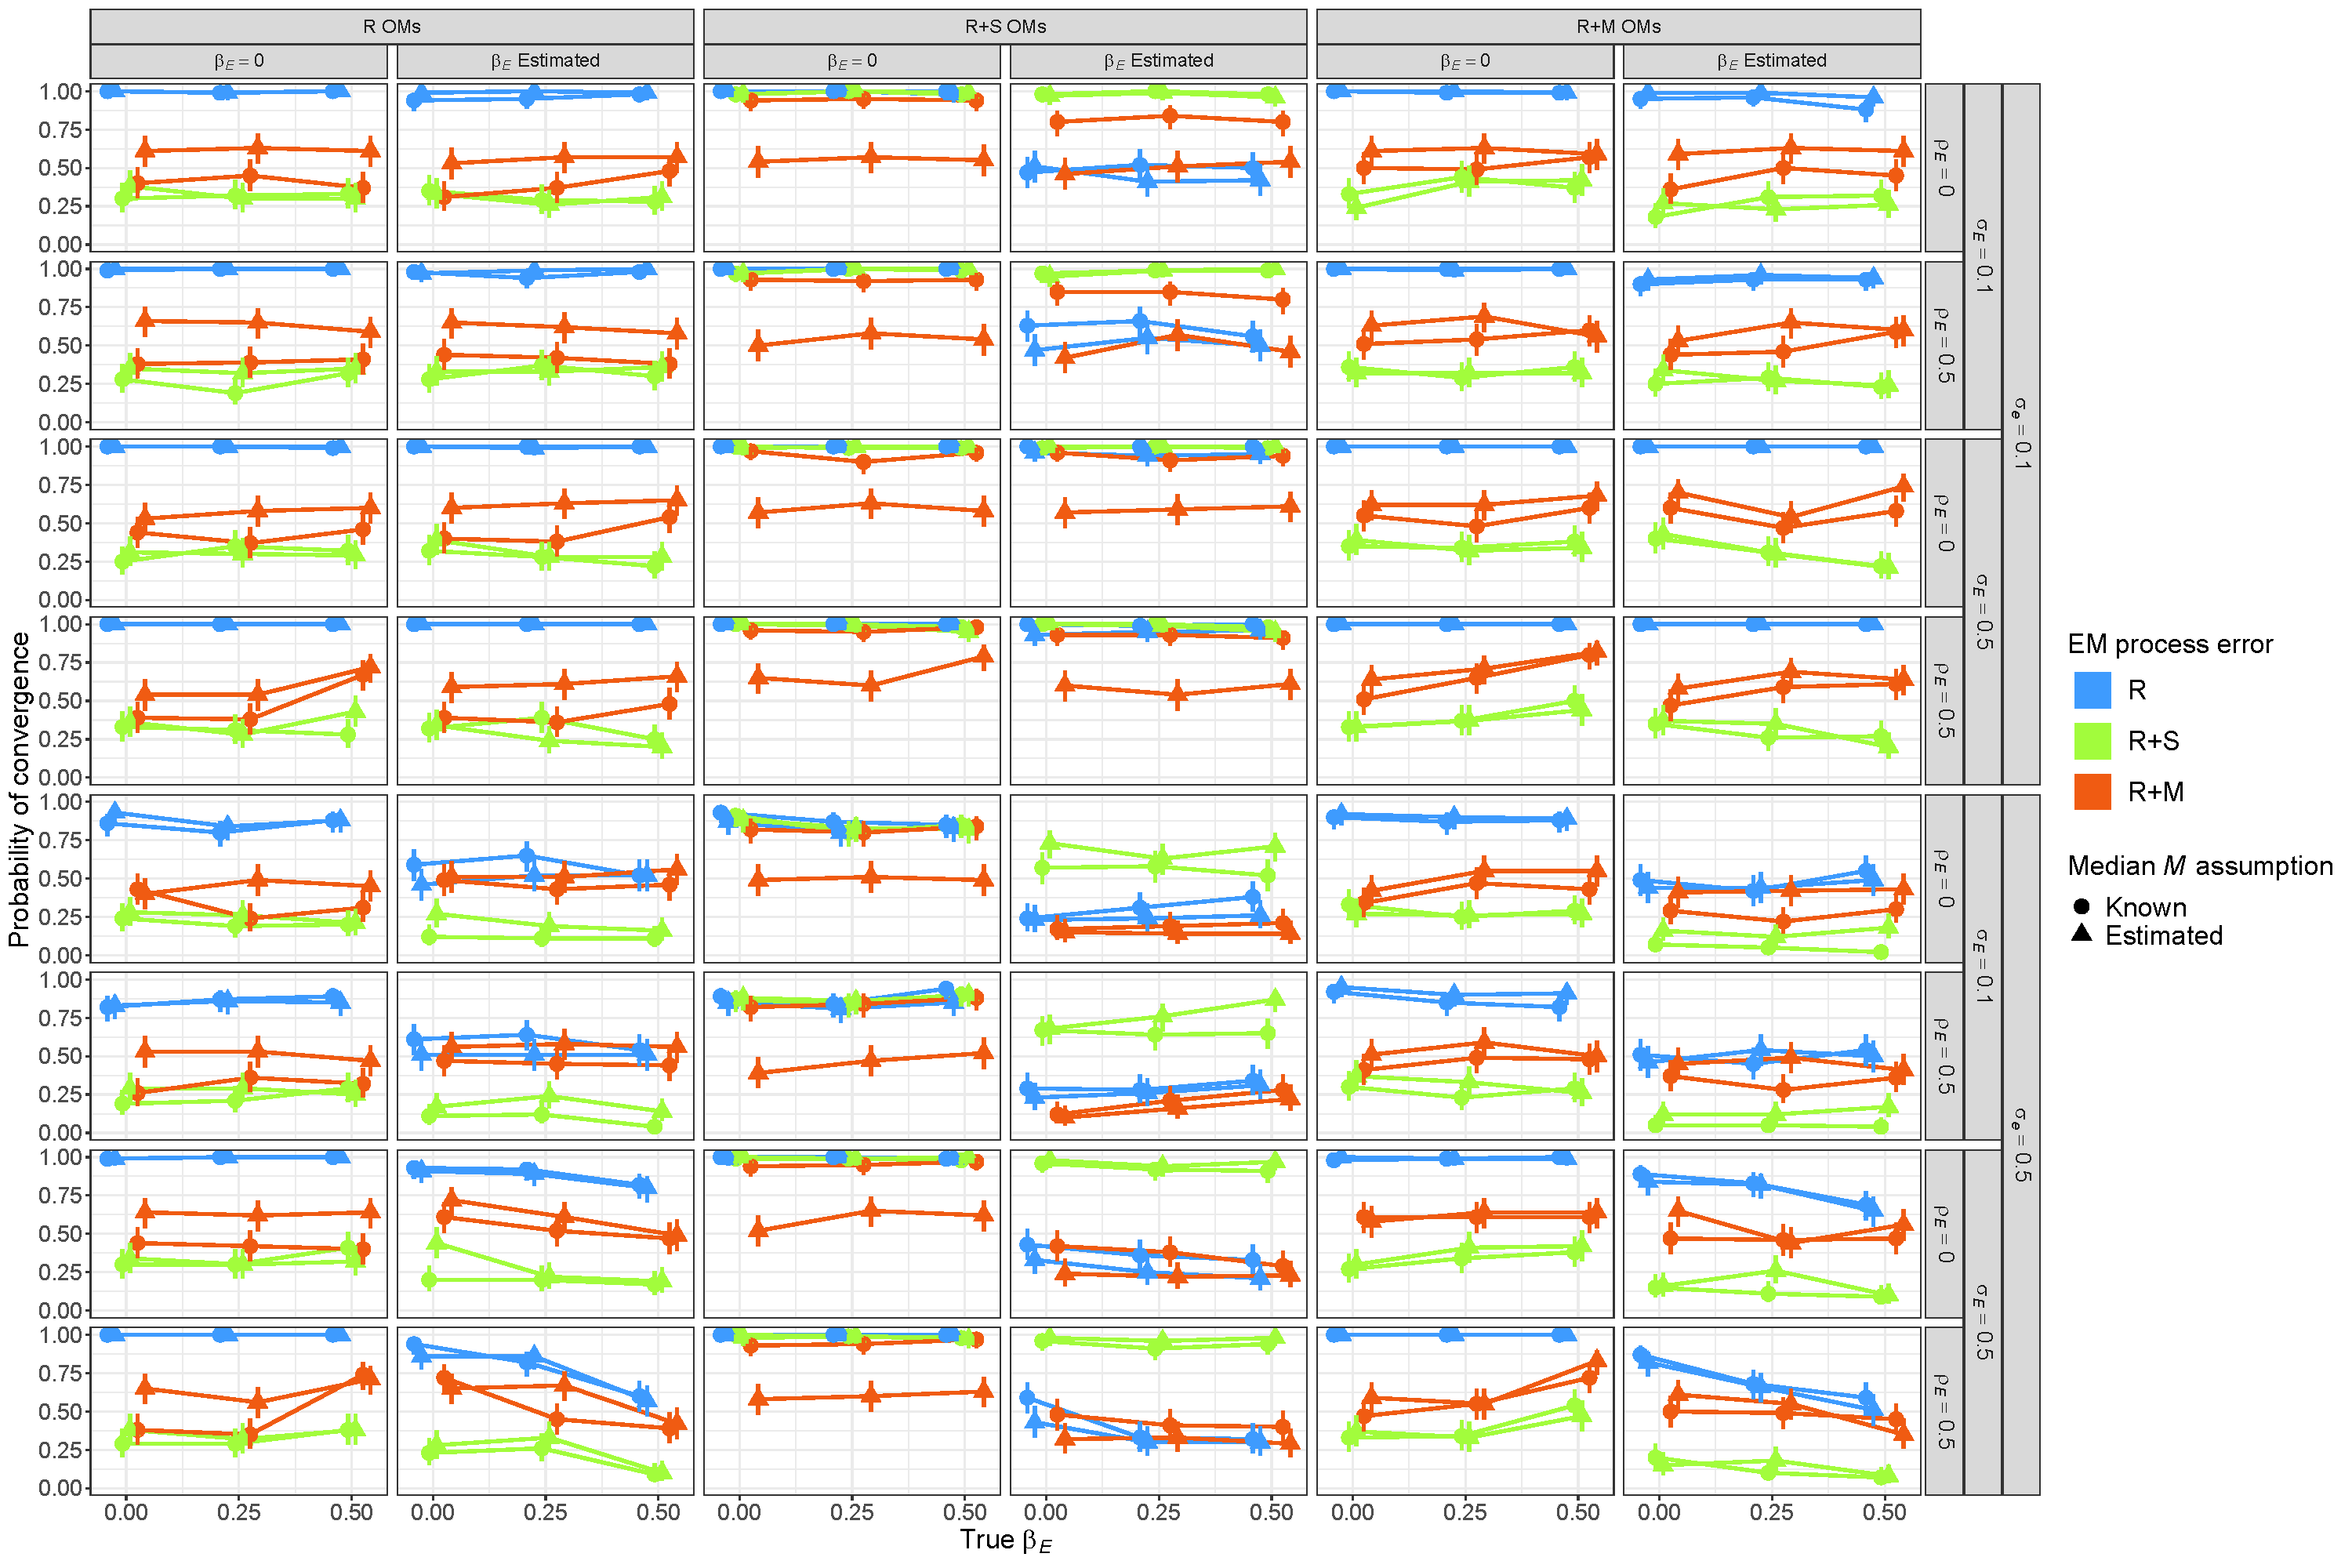
\includegraphics{convergence_main}
%DIFDELCMD < %%%
\DIFdelendFL \DIFaddbeginFL 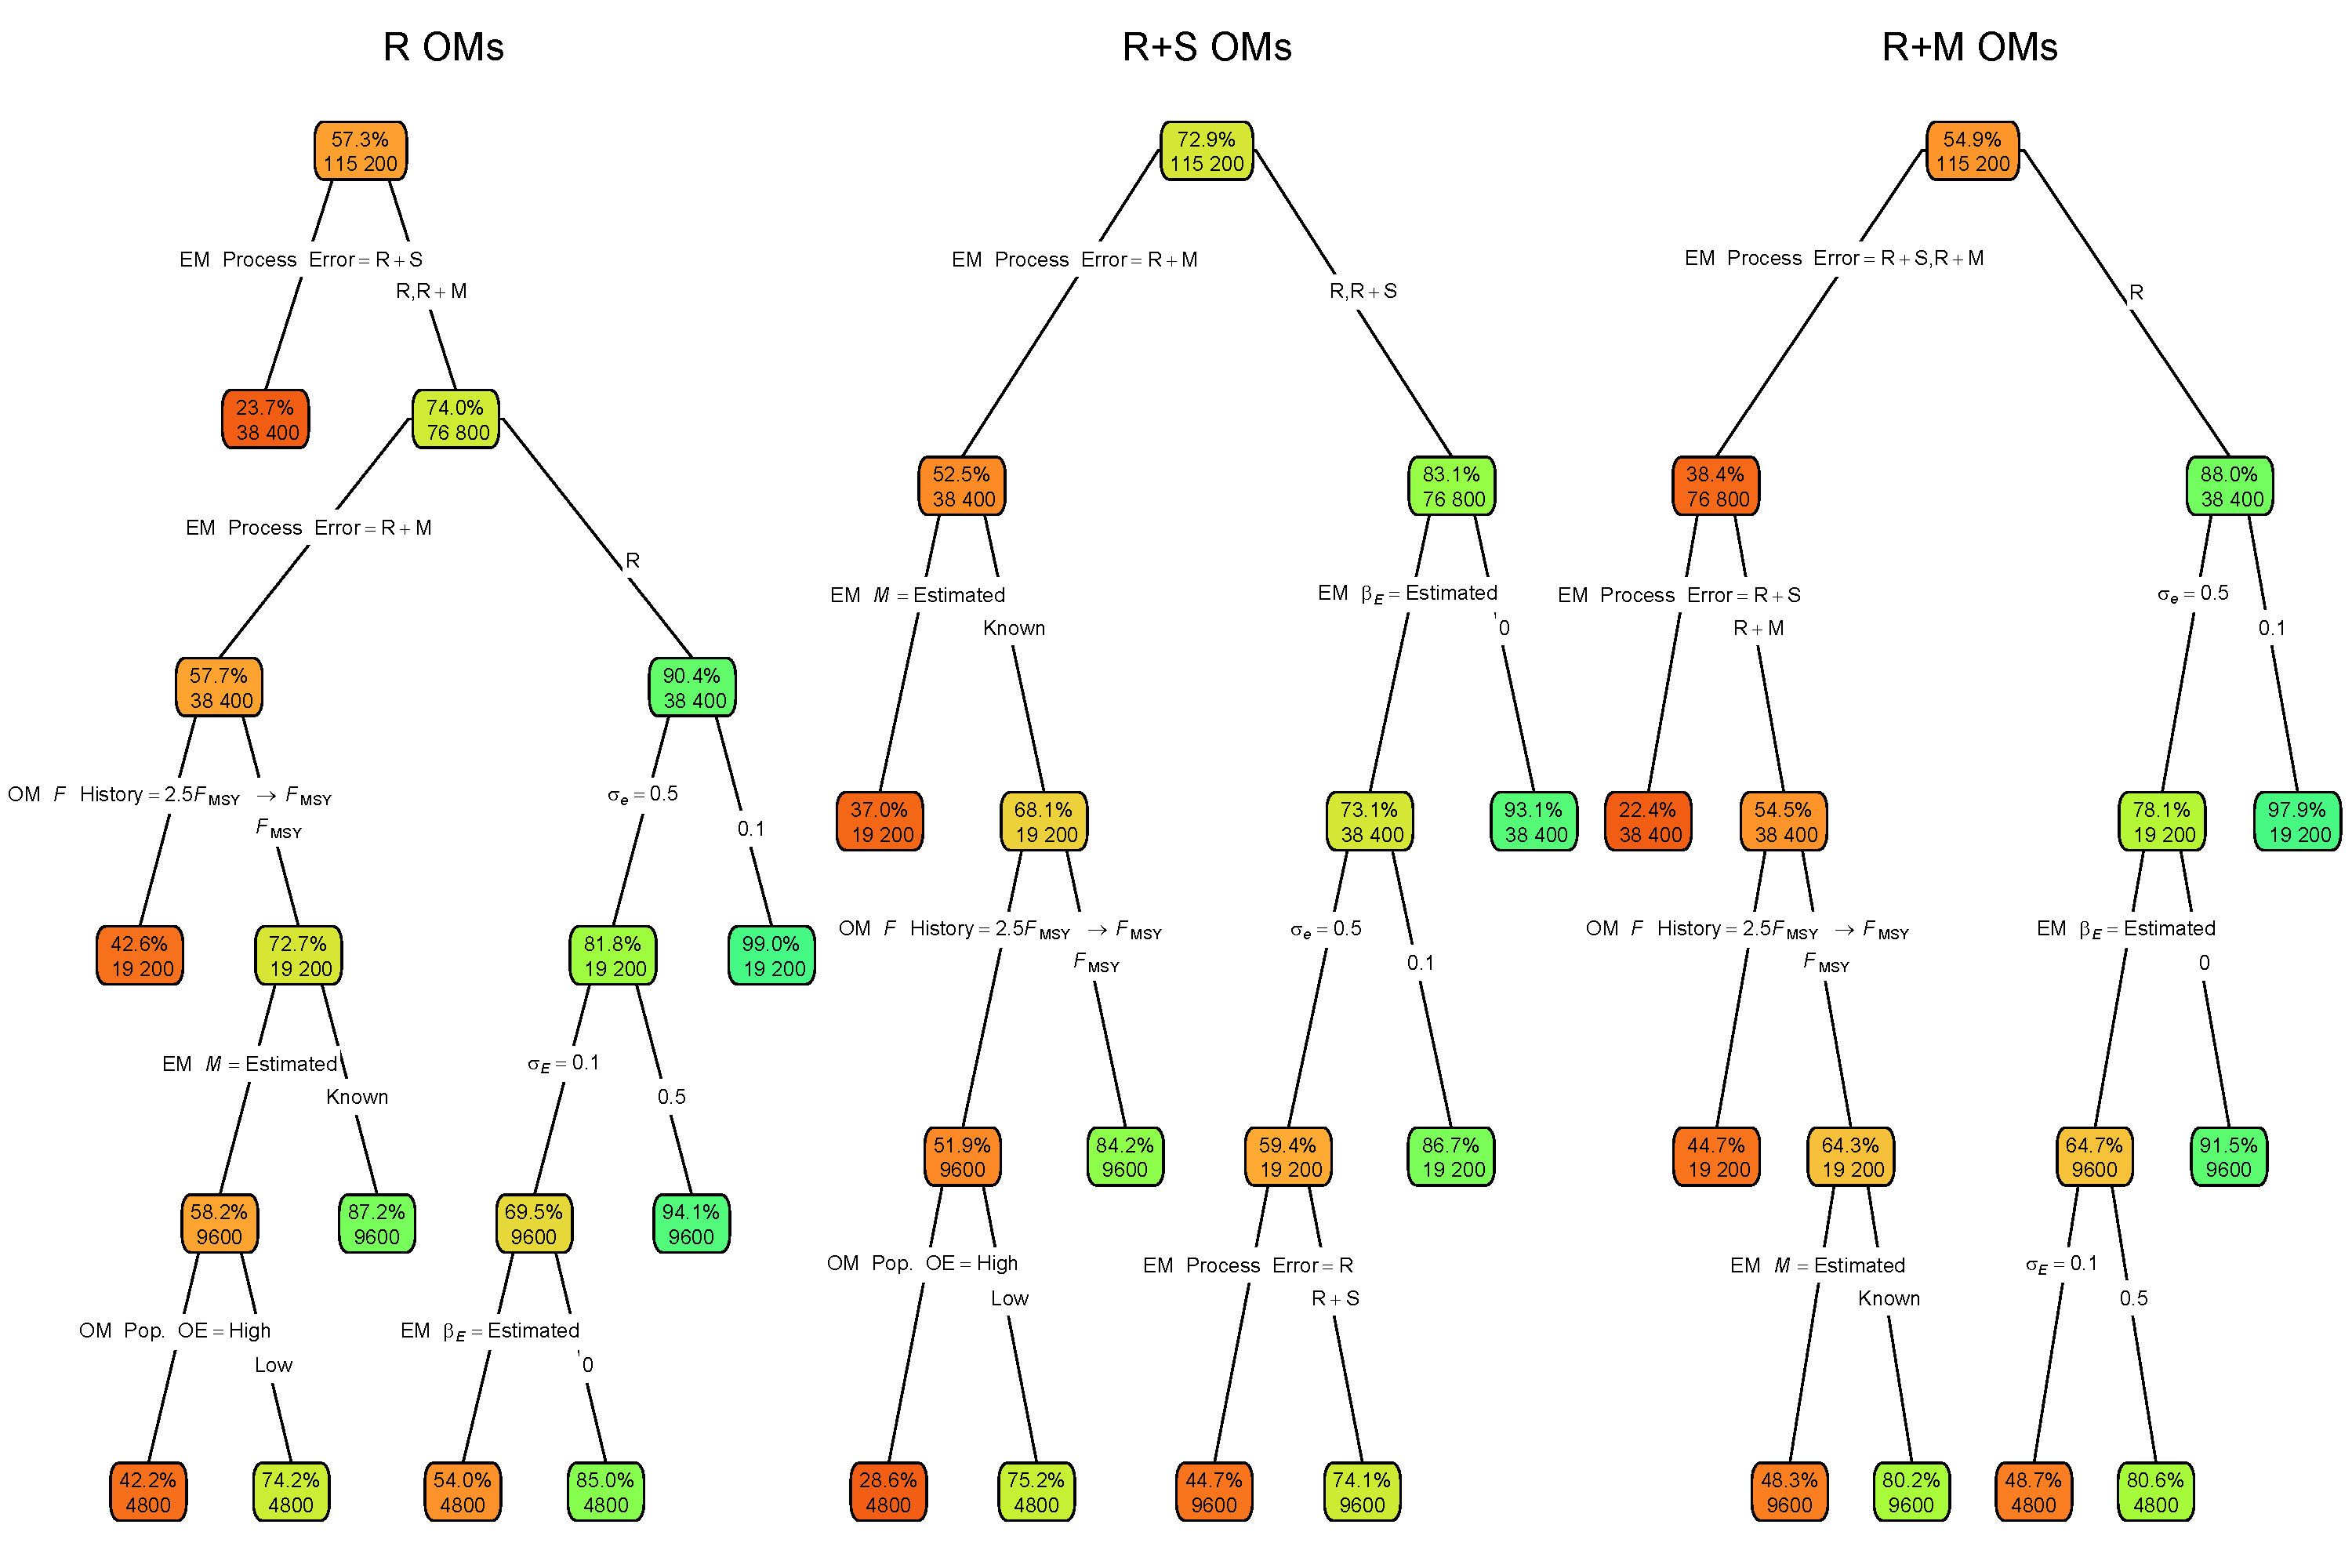
\includegraphics[width = 1.4\textwidth]{convergence_classification_plots}
\DIFaddendFL \end{center}
\caption{\DIFdelbeginFL \DIFdelFL{Estimated probability of fits }\DIFdelendFL \DIFaddbeginFL \DIFaddFL{Classification trees indicating primary factors determining convergence as defined by }\DIFaddendFL providing Hessian-based standard errors for \DIFdelbeginFL \DIFdelFL{EMs }\DIFdelendFL \DIFaddbeginFL \DIFaddFL{operating models (OMs) }\DIFaddendFL with \DIFdelbeginFL \DIFdelFL{alternative }\DIFdelendFL process error \DIFdelbeginFL \DIFdelFL{assumptions, treatment of median natural mortality }\DIFdelendFL \DIFaddbeginFL \DIFaddFL{on recruitment only }\DIFaddendFL (\DIFdelbeginFL \DIFdelFL{$\beta_M$ known or estimated}\DIFdelendFL \DIFaddbeginFL \DIFaddFL{R}\DIFaddendFL ), \DIFaddbeginFL \DIFaddFL{recruitment }\DIFaddendFL and \DIFdelbeginFL \DIFdelFL{treatment of covariate effect }\DIFdelendFL \DIFaddbeginFL \DIFaddFL{apparent survival }\DIFaddendFL (\DIFdelbeginFL \DIFdelFL{$\beta_E = 0$ or estimated). The OMs have }\DIFdelendFL R\DIFdelbeginFL \DIFdelFL{(left) and R}\DIFdelendFL +S\DIFdelbeginFL \DIFdelFL{(middle}\DIFdelendFL ), or \DIFaddbeginFL \DIFaddFL{recruitment and natural mortality (}\DIFaddendFL R+M\DIFdelbeginFL \DIFdelFL{(right}\DIFdelendFL )\DIFdelbeginFL \DIFdelFL{process error structures, alternative configurations of covariate time series structure and levels of observation uncertainty }\DIFdelendFL \DIFaddbeginFL \DIFaddFL{. Nodes denote percent convergence }\DIFaddendFL (\DIFdelbeginFL \DIFdelFL{rows}\DIFdelendFL \DIFaddbeginFL \DIFaddFL{top}\DIFaddendFL ) \DIFdelbeginFL \DIFdelFL{, }\DIFdelendFL and \DIFdelbeginFL \DIFdelFL{three levels }\DIFdelendFL \DIFaddbeginFL \DIFaddFL{number }\DIFaddendFL of \DIFdelbeginFL \DIFdelFL{true covariate effect on median natural mortality }\DIFdelendFL \DIFaddbeginFL \DIFaddFL{fits }\DIFaddendFL (\DIFdelbeginFL \DIFdelFL{x axis}\DIFdelendFL \DIFaddbeginFL \DIFaddFL{bottom}\DIFaddendFL ) \DIFaddbeginFL \DIFaddFL{for the corresponding subset}\DIFaddendFL . \DIFdelbeginFL \DIFdelFL{All OMs had low observation error }\DIFdelendFL \DIFaddbeginFL \DIFaddFL{Lower or higher convergence rates are indicated by more red or green polygons, respectively. See Table \ref{factor_table} }\DIFaddendFL for \DIFdelbeginFL \DIFdelFL{fish population observations }\DIFdelendFL \DIFaddbeginFL \DIFaddFL{description of OM }\DIFaddendFL and \DIFdelbeginFL \DIFdelFL{temporal contrast in fishing pressure}\DIFdelendFL \DIFaddbeginFL \DIFaddFL{EM factors defining nodes and branches}\DIFaddendFL .\DIFdelbeginFL \DIFdelFL{Vertical lines represent 95\% confidence intervals.}\DIFdelendFL }\DIFdelbeginFL %DIFDELCMD < \label{convergence}
%DIFDELCMD < %%%
\DIFdelendFL \DIFaddbeginFL \label{conv_class}
\DIFaddendFL \end{figure}
\end{landscape}

\begin{landscape}
\begin{figure}
\begin{center}
\DIFdelbeginFL %DIFDELCMD < 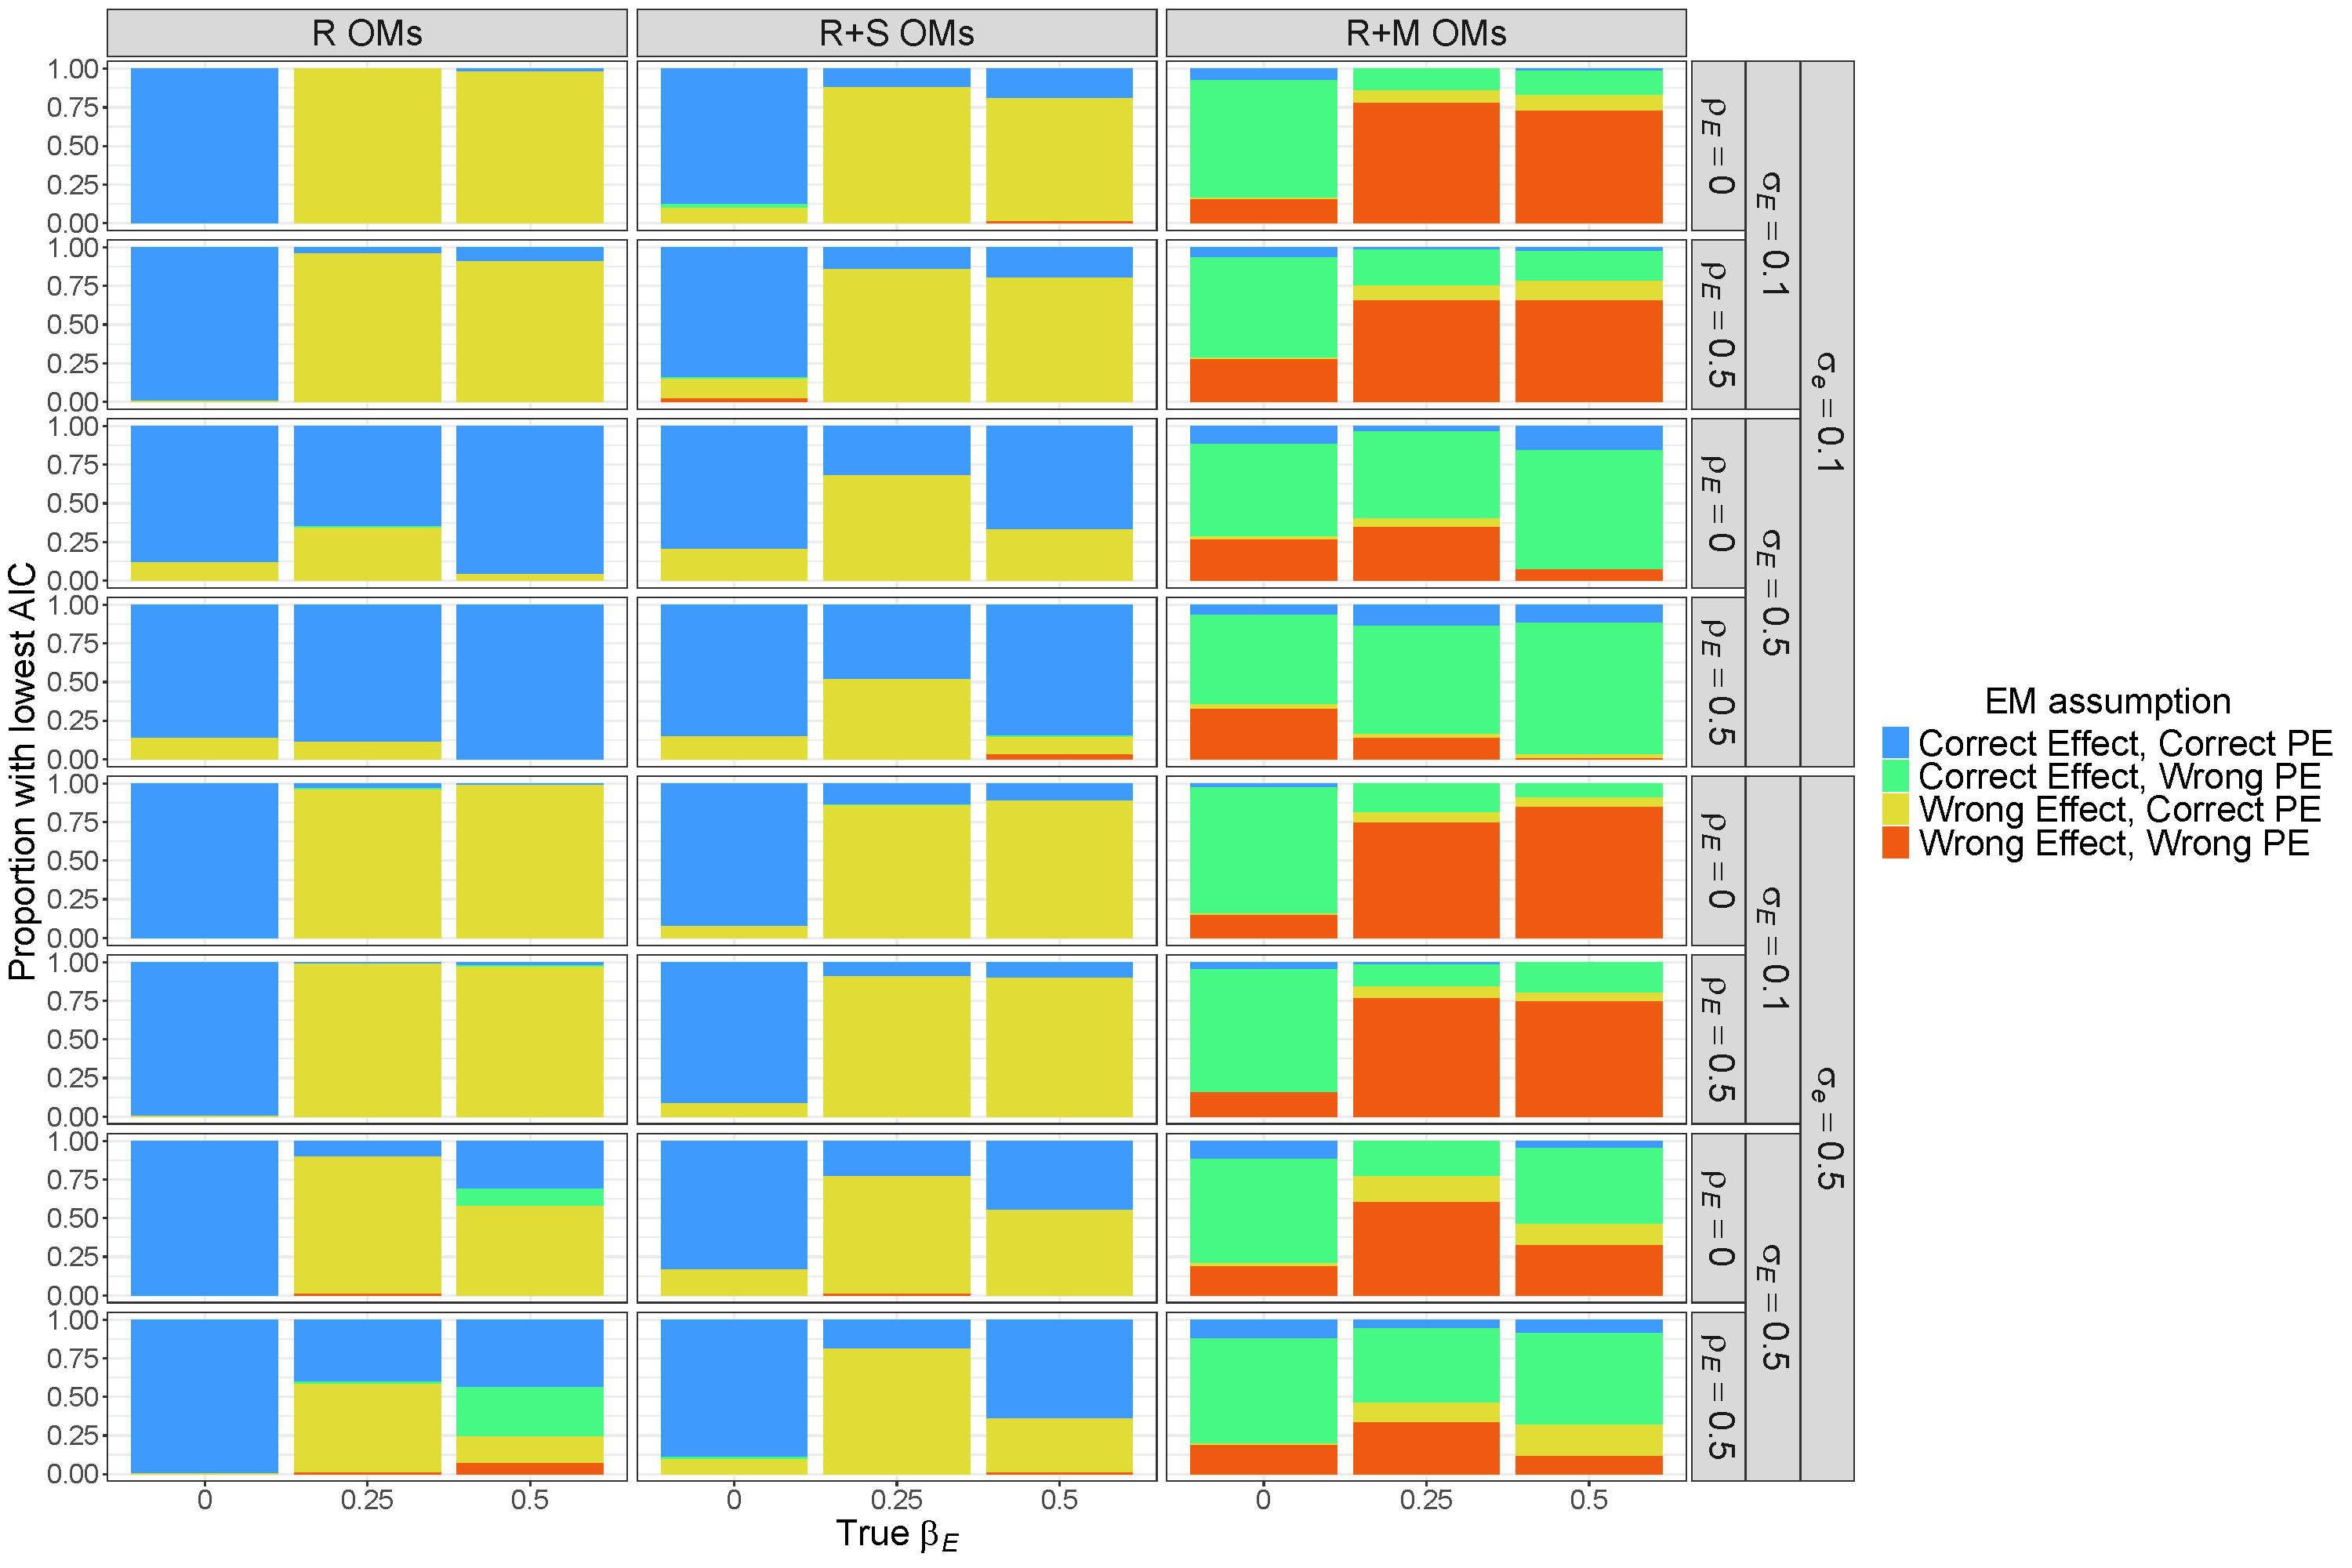
\includegraphics[height = \textheight]{aic_main}
%DIFDELCMD < %%%
\DIFdelendFL \DIFaddbeginFL 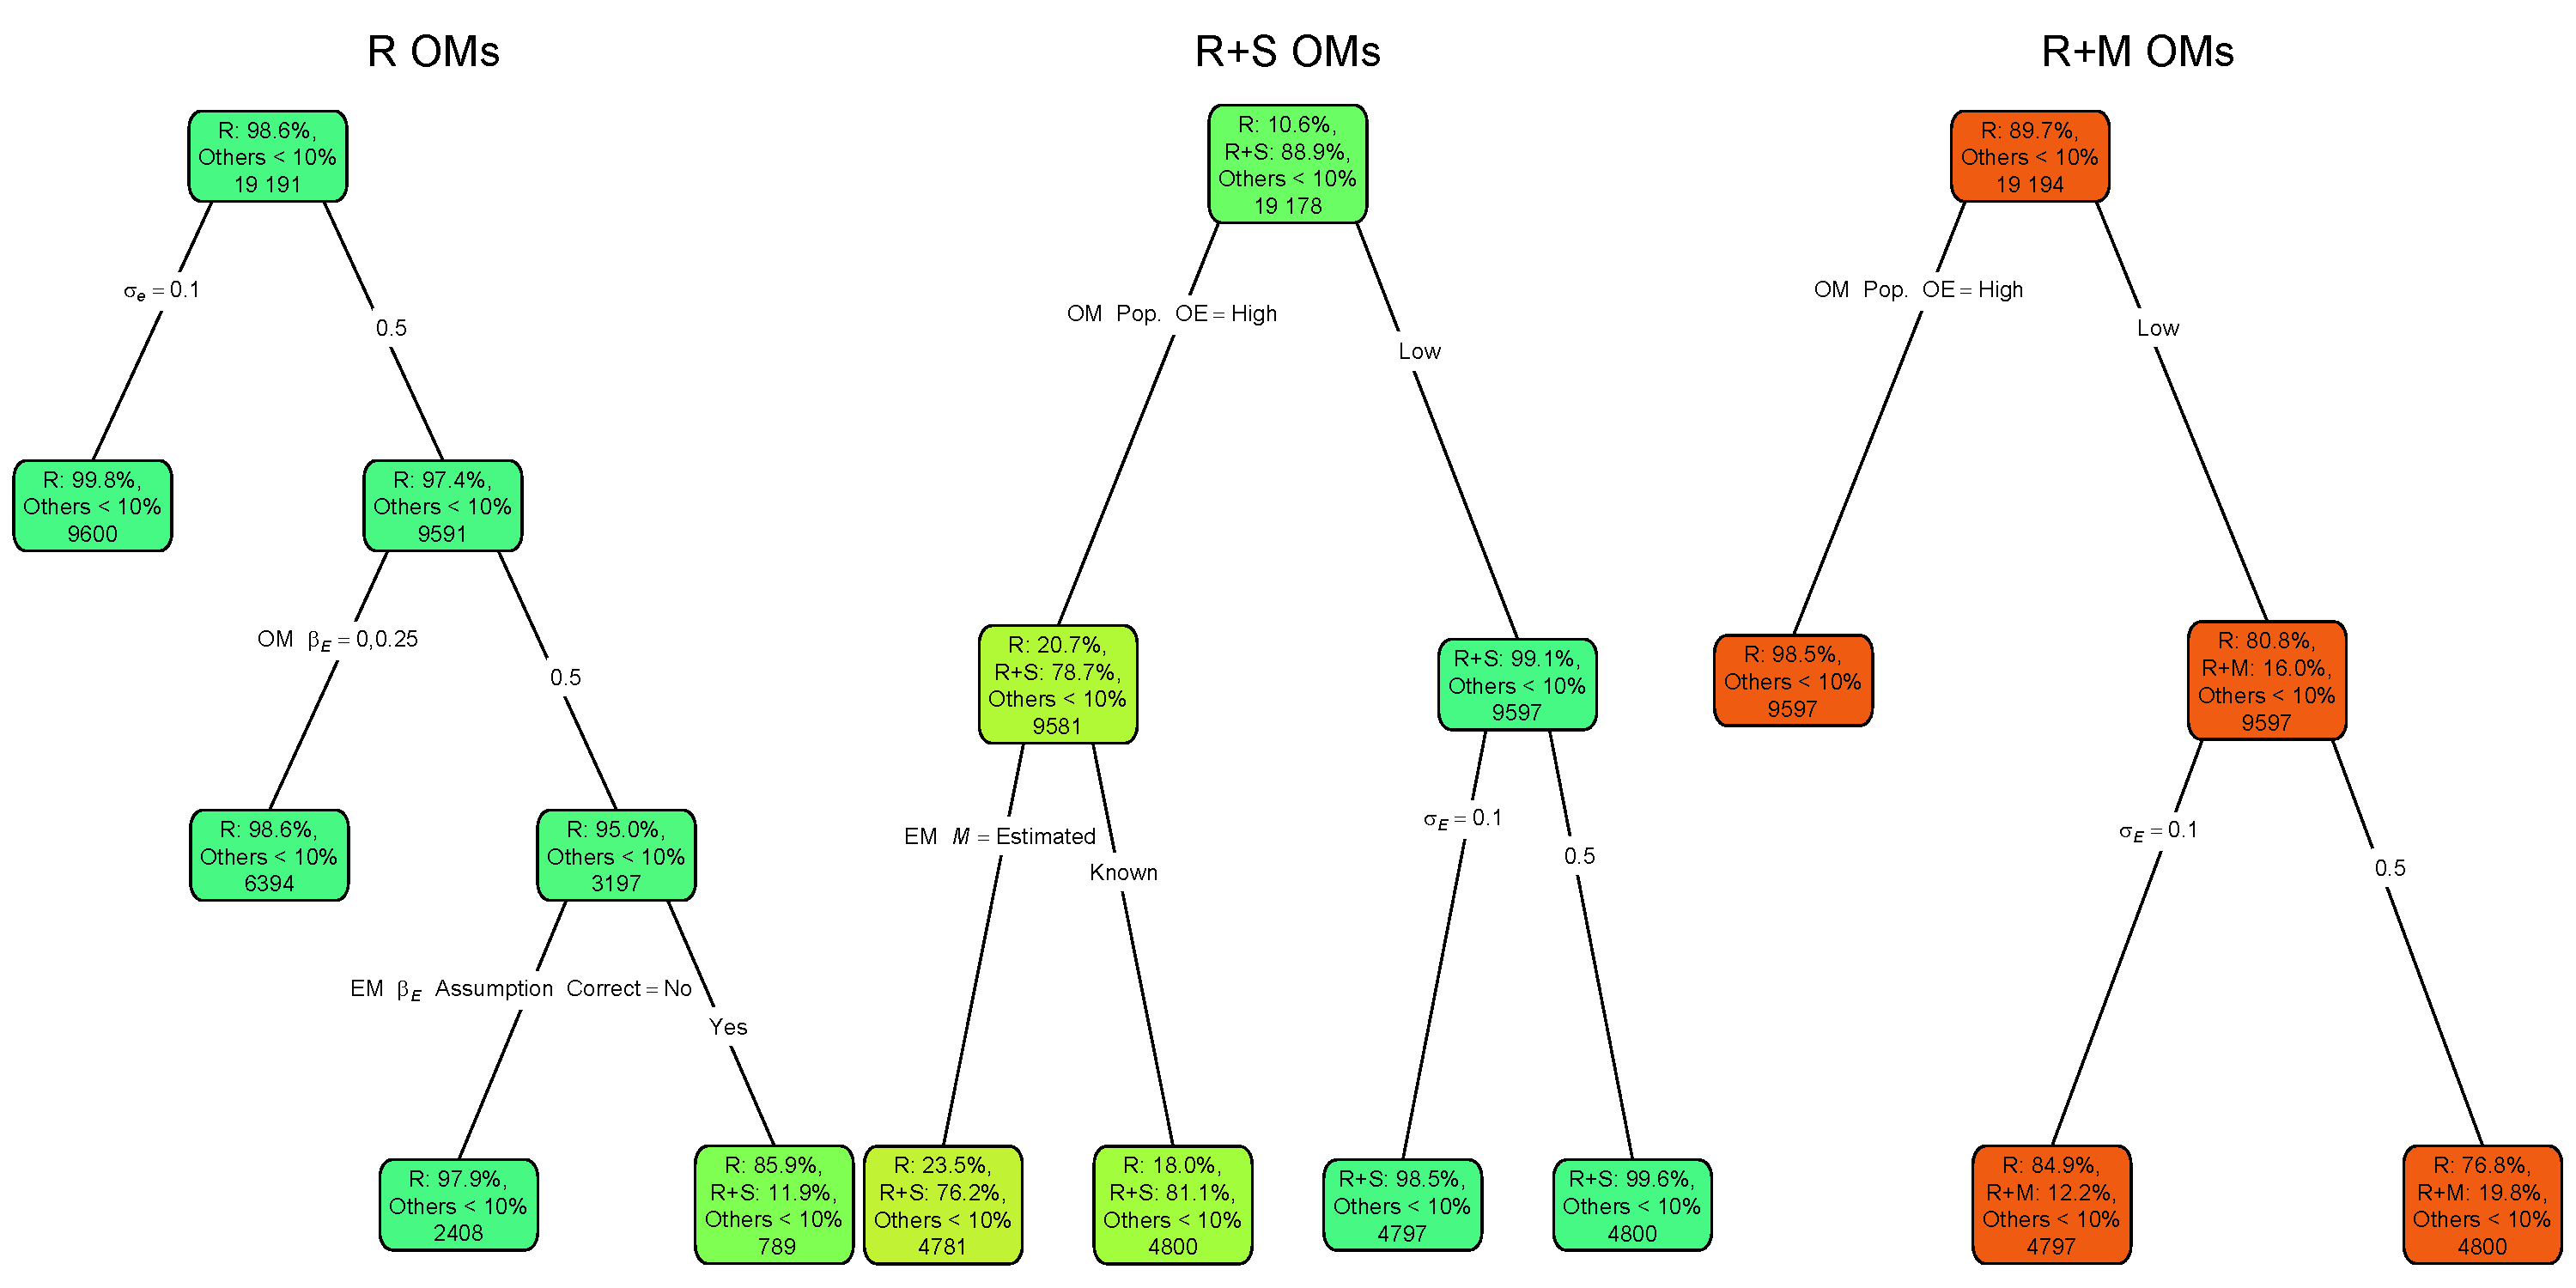
\includegraphics[width = 1.4\textwidth]{AIC_PE_classification_plots}
\DIFaddendFL \end{center}
\caption{\DIFdelbeginFL \DIFdelFL{For each OM}\DIFdelendFL \DIFaddbeginFL \DIFaddFL{Classification trees indicating primary factors determining which process error assumption in estimating models (EMs) provides the lowest AIC for operating models (OMs) with process error on recruitment only (R)}\DIFaddendFL , \DIFaddbeginFL \DIFaddFL{recruitment and apparent survival (R+S), or recruitment and natural mortality (R+M). Each node shows }\DIFaddendFL the \DIFdelbeginFL \DIFdelFL{proportion }\DIFdelendFL \DIFaddbeginFL \DIFaddFL{percentage }\DIFaddendFL of \DIFdelbeginFL \DIFdelFL{simulated data sets where the }\DIFdelendFL EM \DIFdelbeginFL \DIFdelFL{type (treatment of environmental covariate effect and  assumed }\DIFdelendFL \DIFaddbeginFL \DIFaddFL{fits with a given }\DIFaddendFL process error \DIFdelbeginFL \DIFdelFL{type) had }\DIFdelendFL \DIFaddbeginFL \DIFaddFL{assumption having }\DIFaddendFL the lowest AIC \DIFaddbeginFL \DIFaddFL{and the number of observations for the corresponding subset of fits}\DIFaddendFL . \DIFdelbeginFL \DIFdelFL{All OMs had low observation }\DIFdelendFL \DIFaddbeginFL \DIFaddFL{Lower or higher accuracy of the process }\DIFaddendFL error \DIFaddbeginFL \DIFaddFL{assumption are indicated by more red or green polygons, respectively. See Table \ref{factor_table} }\DIFaddendFL for \DIFdelbeginFL \DIFdelFL{fish population observations }\DIFdelendFL \DIFaddbeginFL \DIFaddFL{description of OM }\DIFaddendFL and \DIFdelbeginFL \DIFdelFL{temporal contrast in fishing pressure}\DIFdelendFL \DIFaddbeginFL \DIFaddFL{EM factors defining nodes and branches}\DIFaddendFL .\DIFdelbeginFL \DIFdelFL{All EMs estimated median natural mortality rate.}\DIFdelendFL }\DIFdelbeginFL %DIFDELCMD < \label{aic}
%DIFDELCMD < %%%
\DIFdelendFL \DIFaddbeginFL \label{AIC_PE_class}
\DIFaddendFL \end{figure}
\end{landscape}

\begin{landscape}
\begin{figure}
\begin{center}
\DIFdelbeginFL %DIFDELCMD < 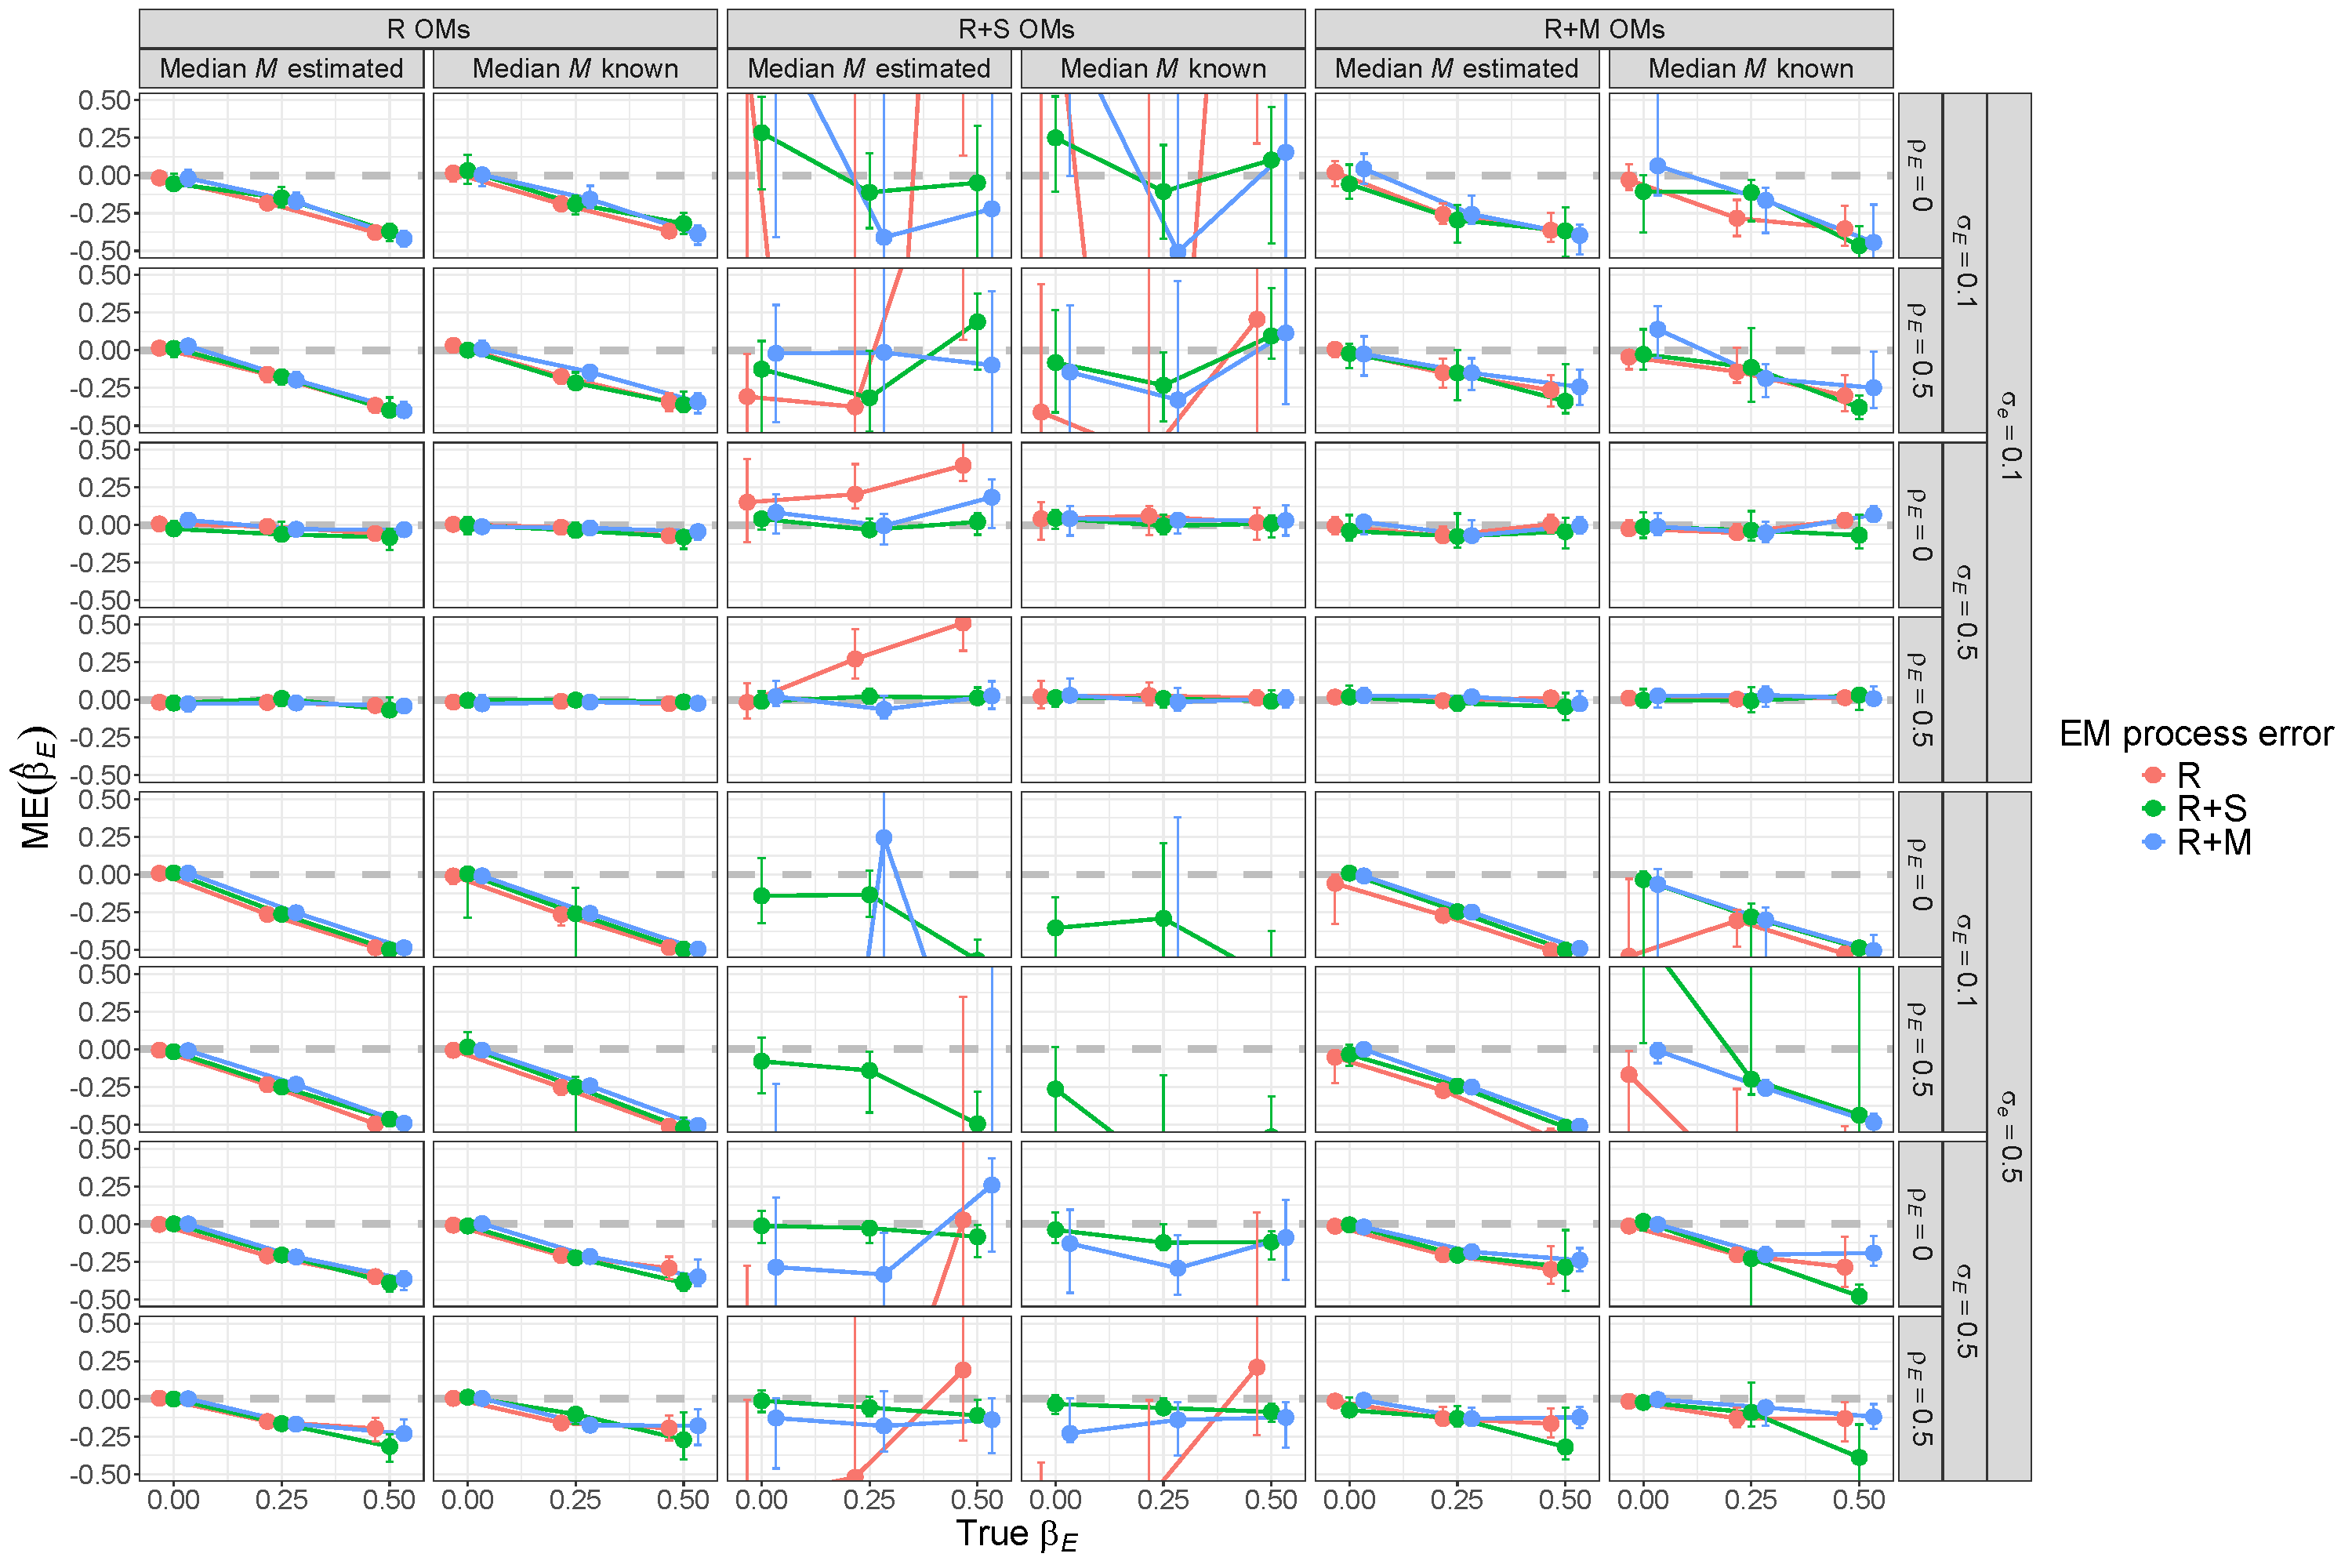
\includegraphics[height = \textheight]{beta_E_bias_main}
%DIFDELCMD < %%%
\DIFdelendFL \DIFaddbeginFL 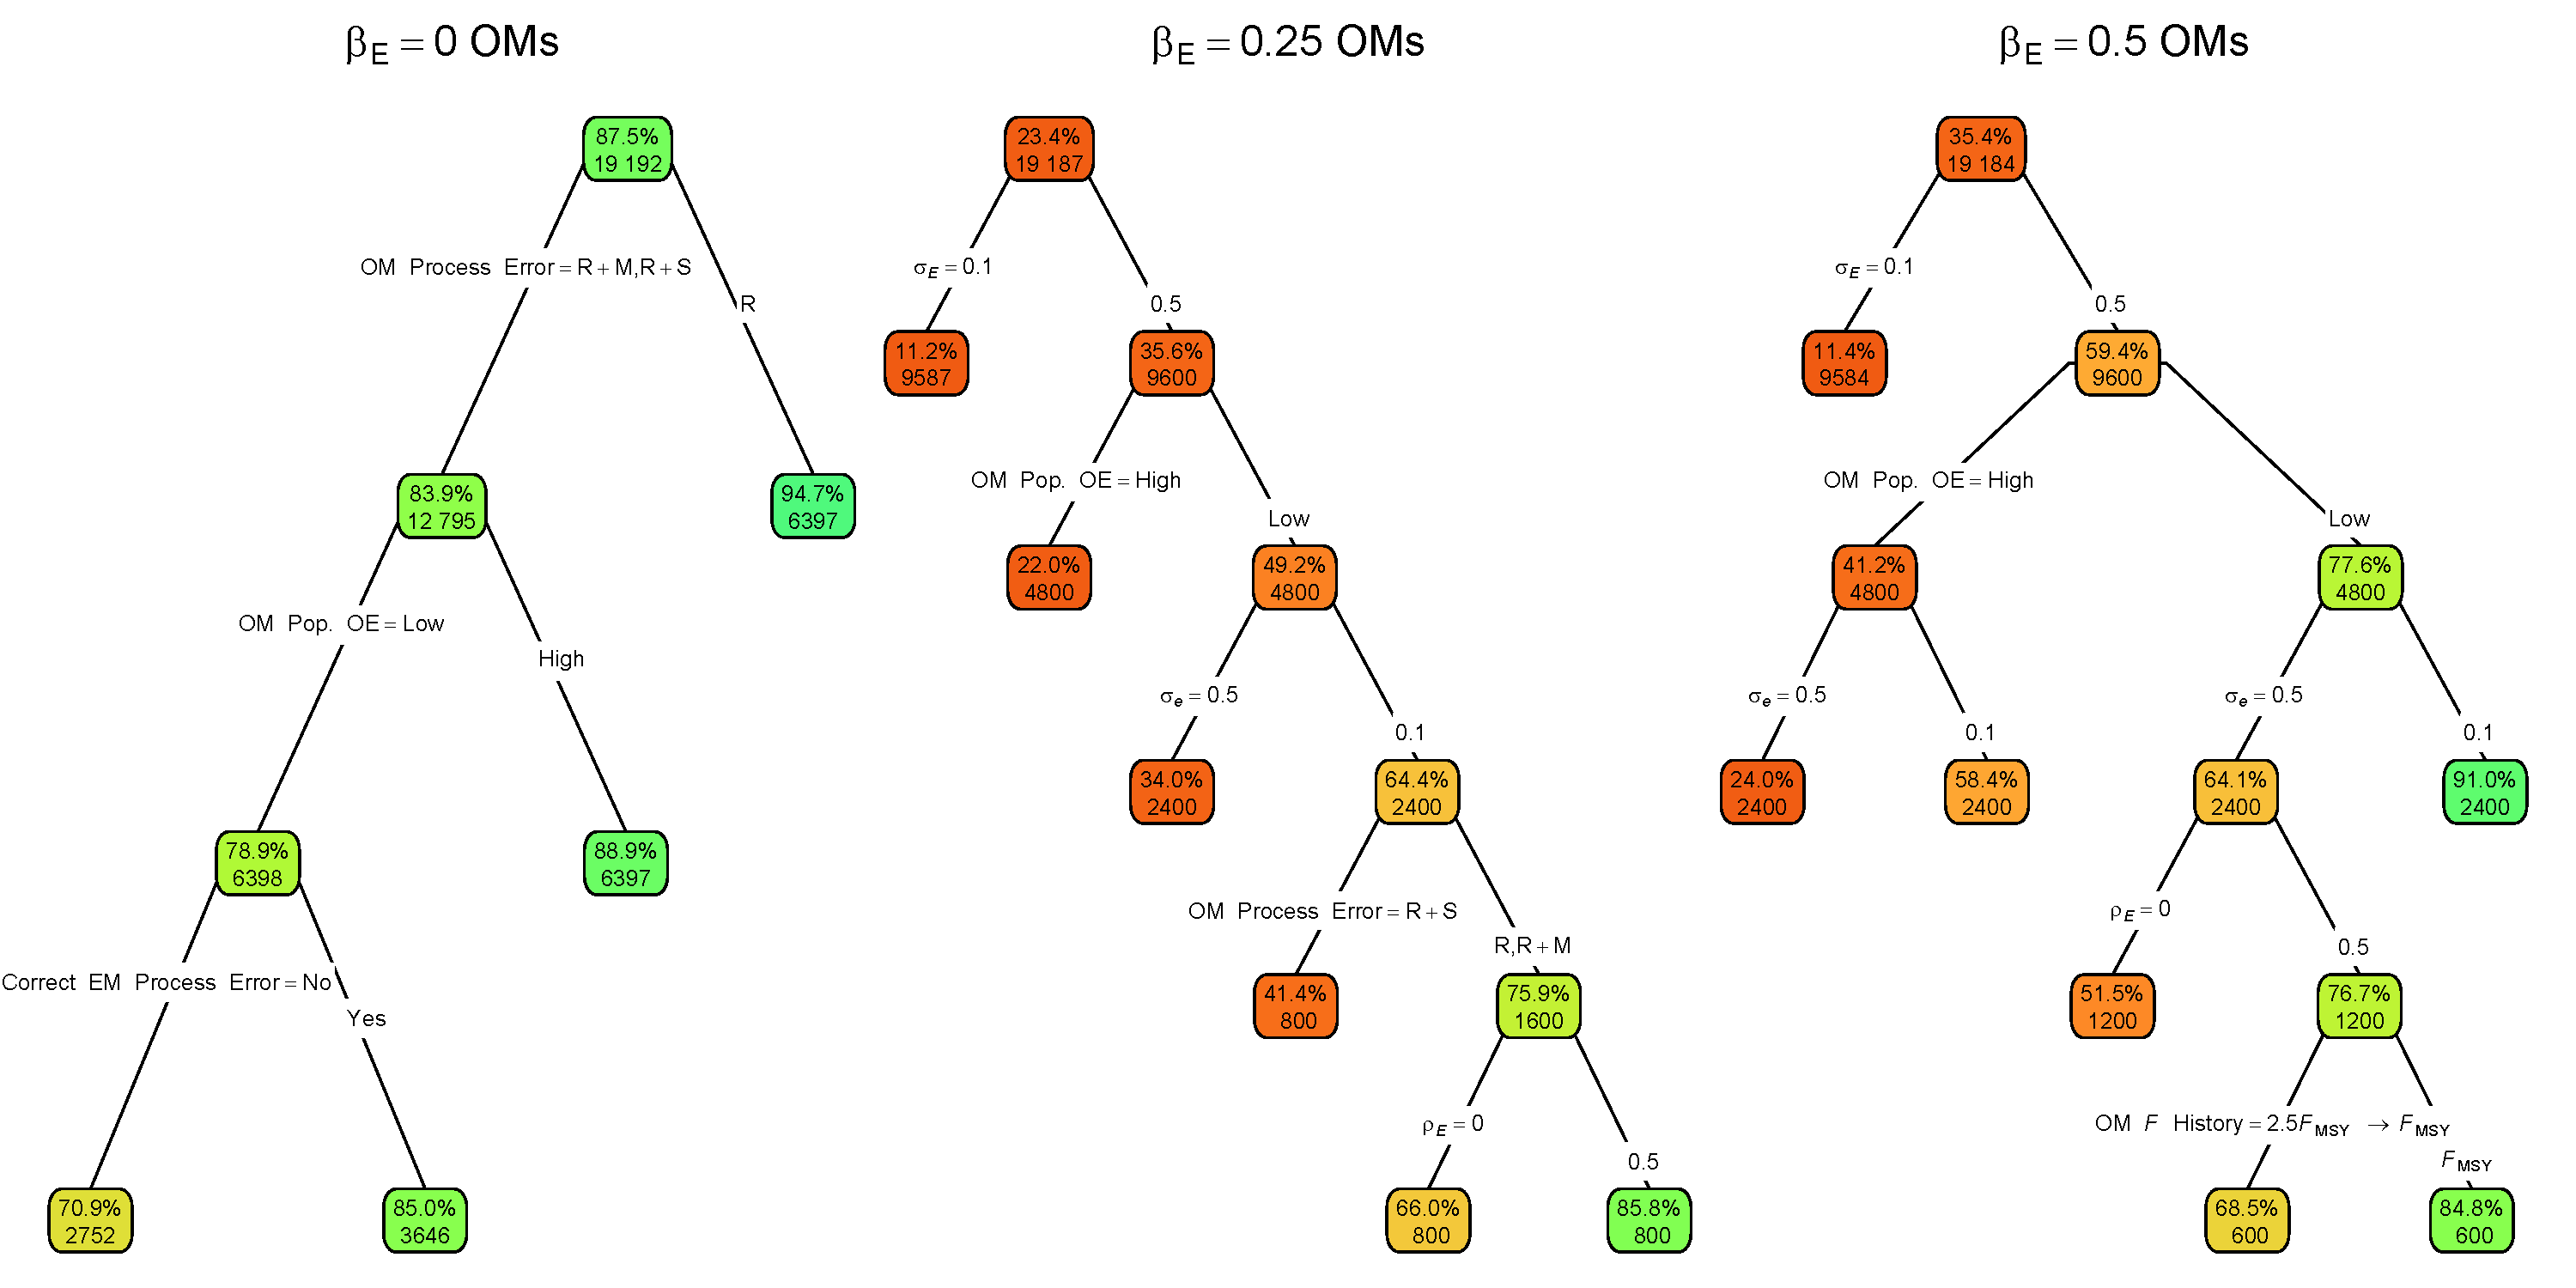
\includegraphics[width = 1.4\textwidth]{AIC_Ecov_effect_classification_plots}
\DIFaddendFL \end{center}
\caption{\DIFdelbeginFL \DIFdelFL{Median error }\DIFdelendFL \DIFaddbeginFL \DIFaddFL{Classification trees indicating primary factors determining whether the correct EM assumption for covariate effect on $M$ }\DIFaddendFL (\DIFdelbeginFL \DIFdelFL{ME}\DIFdelendFL \DIFaddbeginFL \DIFaddFL{no effect with OM $\beta_E = 0$ or estimated effect when OM $\beta_E > 0$}\DIFaddendFL ) \DIFaddbeginFL \DIFaddFL{provides the lowest AIC for OMs assuming values for $\beta_E$ }\DIFaddendFL of \DIFdelbeginFL \DIFdelFL{estimates }\DIFdelendFL \DIFaddbeginFL \DIFaddFL{0, 0.25, and 0.5. Nodes denote the percentage }\DIFaddendFL of \DIFdelbeginFL \DIFdelFL{environmental effect on natural mortality $\beta_E$ from fitting }\DIFdelendFL \DIFaddbeginFL \DIFaddFL{estimating models (}\DIFaddendFL EMs\DIFaddbeginFL \DIFaddFL{) }\DIFaddendFL with \DIFdelbeginFL \DIFdelFL{alternative process error assumptions }\DIFdelendFL \DIFaddbeginFL \DIFaddFL{correct assumption }\DIFaddendFL and \DIFdelbeginFL \DIFdelFL{treatment }\DIFdelendFL \DIFaddbeginFL \DIFaddFL{lowest AIC (top), and number }\DIFaddendFL of \DIFdelbeginFL \DIFdelFL{median natural mortality }\DIFdelendFL \DIFaddbeginFL \DIFaddFL{observations }\DIFaddendFL (\DIFdelbeginFL \DIFdelFL{$\beta_M$ known or estimated}\DIFdelendFL \DIFaddbeginFL \DIFaddFL{bottom}\DIFaddendFL ) \DIFaddbeginFL \DIFaddFL{for the corresponding subset}\DIFaddendFL . \DIFdelbeginFL \DIFdelFL{All OMs had low observation }\DIFdelendFL \DIFaddbeginFL \DIFaddFL{Lower or higher accuracy of the process }\DIFaddendFL error \DIFaddbeginFL \DIFaddFL{assumption are indicated by more red or green polygons, respectively. See Table \ref{factor_table} for description of OM }\DIFaddendFL and \DIFdelbeginFL \DIFdelFL{contrast in fishing mortality}\DIFdelendFL \DIFaddbeginFL \DIFaddFL{EM factors defining nodes and branches}\DIFaddendFL .\DIFdelbeginFL \DIFdelFL{Vertical lines represent 95\% confidence intervals.}\DIFdelendFL }\DIFdelbeginFL %DIFDELCMD < \label{beta_E_bias}
%DIFDELCMD < %%%
\DIFdelendFL \DIFaddbeginFL \label{AIC_Ecov_effect_class}
\DIFaddendFL \end{figure}
\end{landscape}

\begin{landscape}
\begin{figure}
\begin{center}
\DIFdelbeginFL %DIFDELCMD < 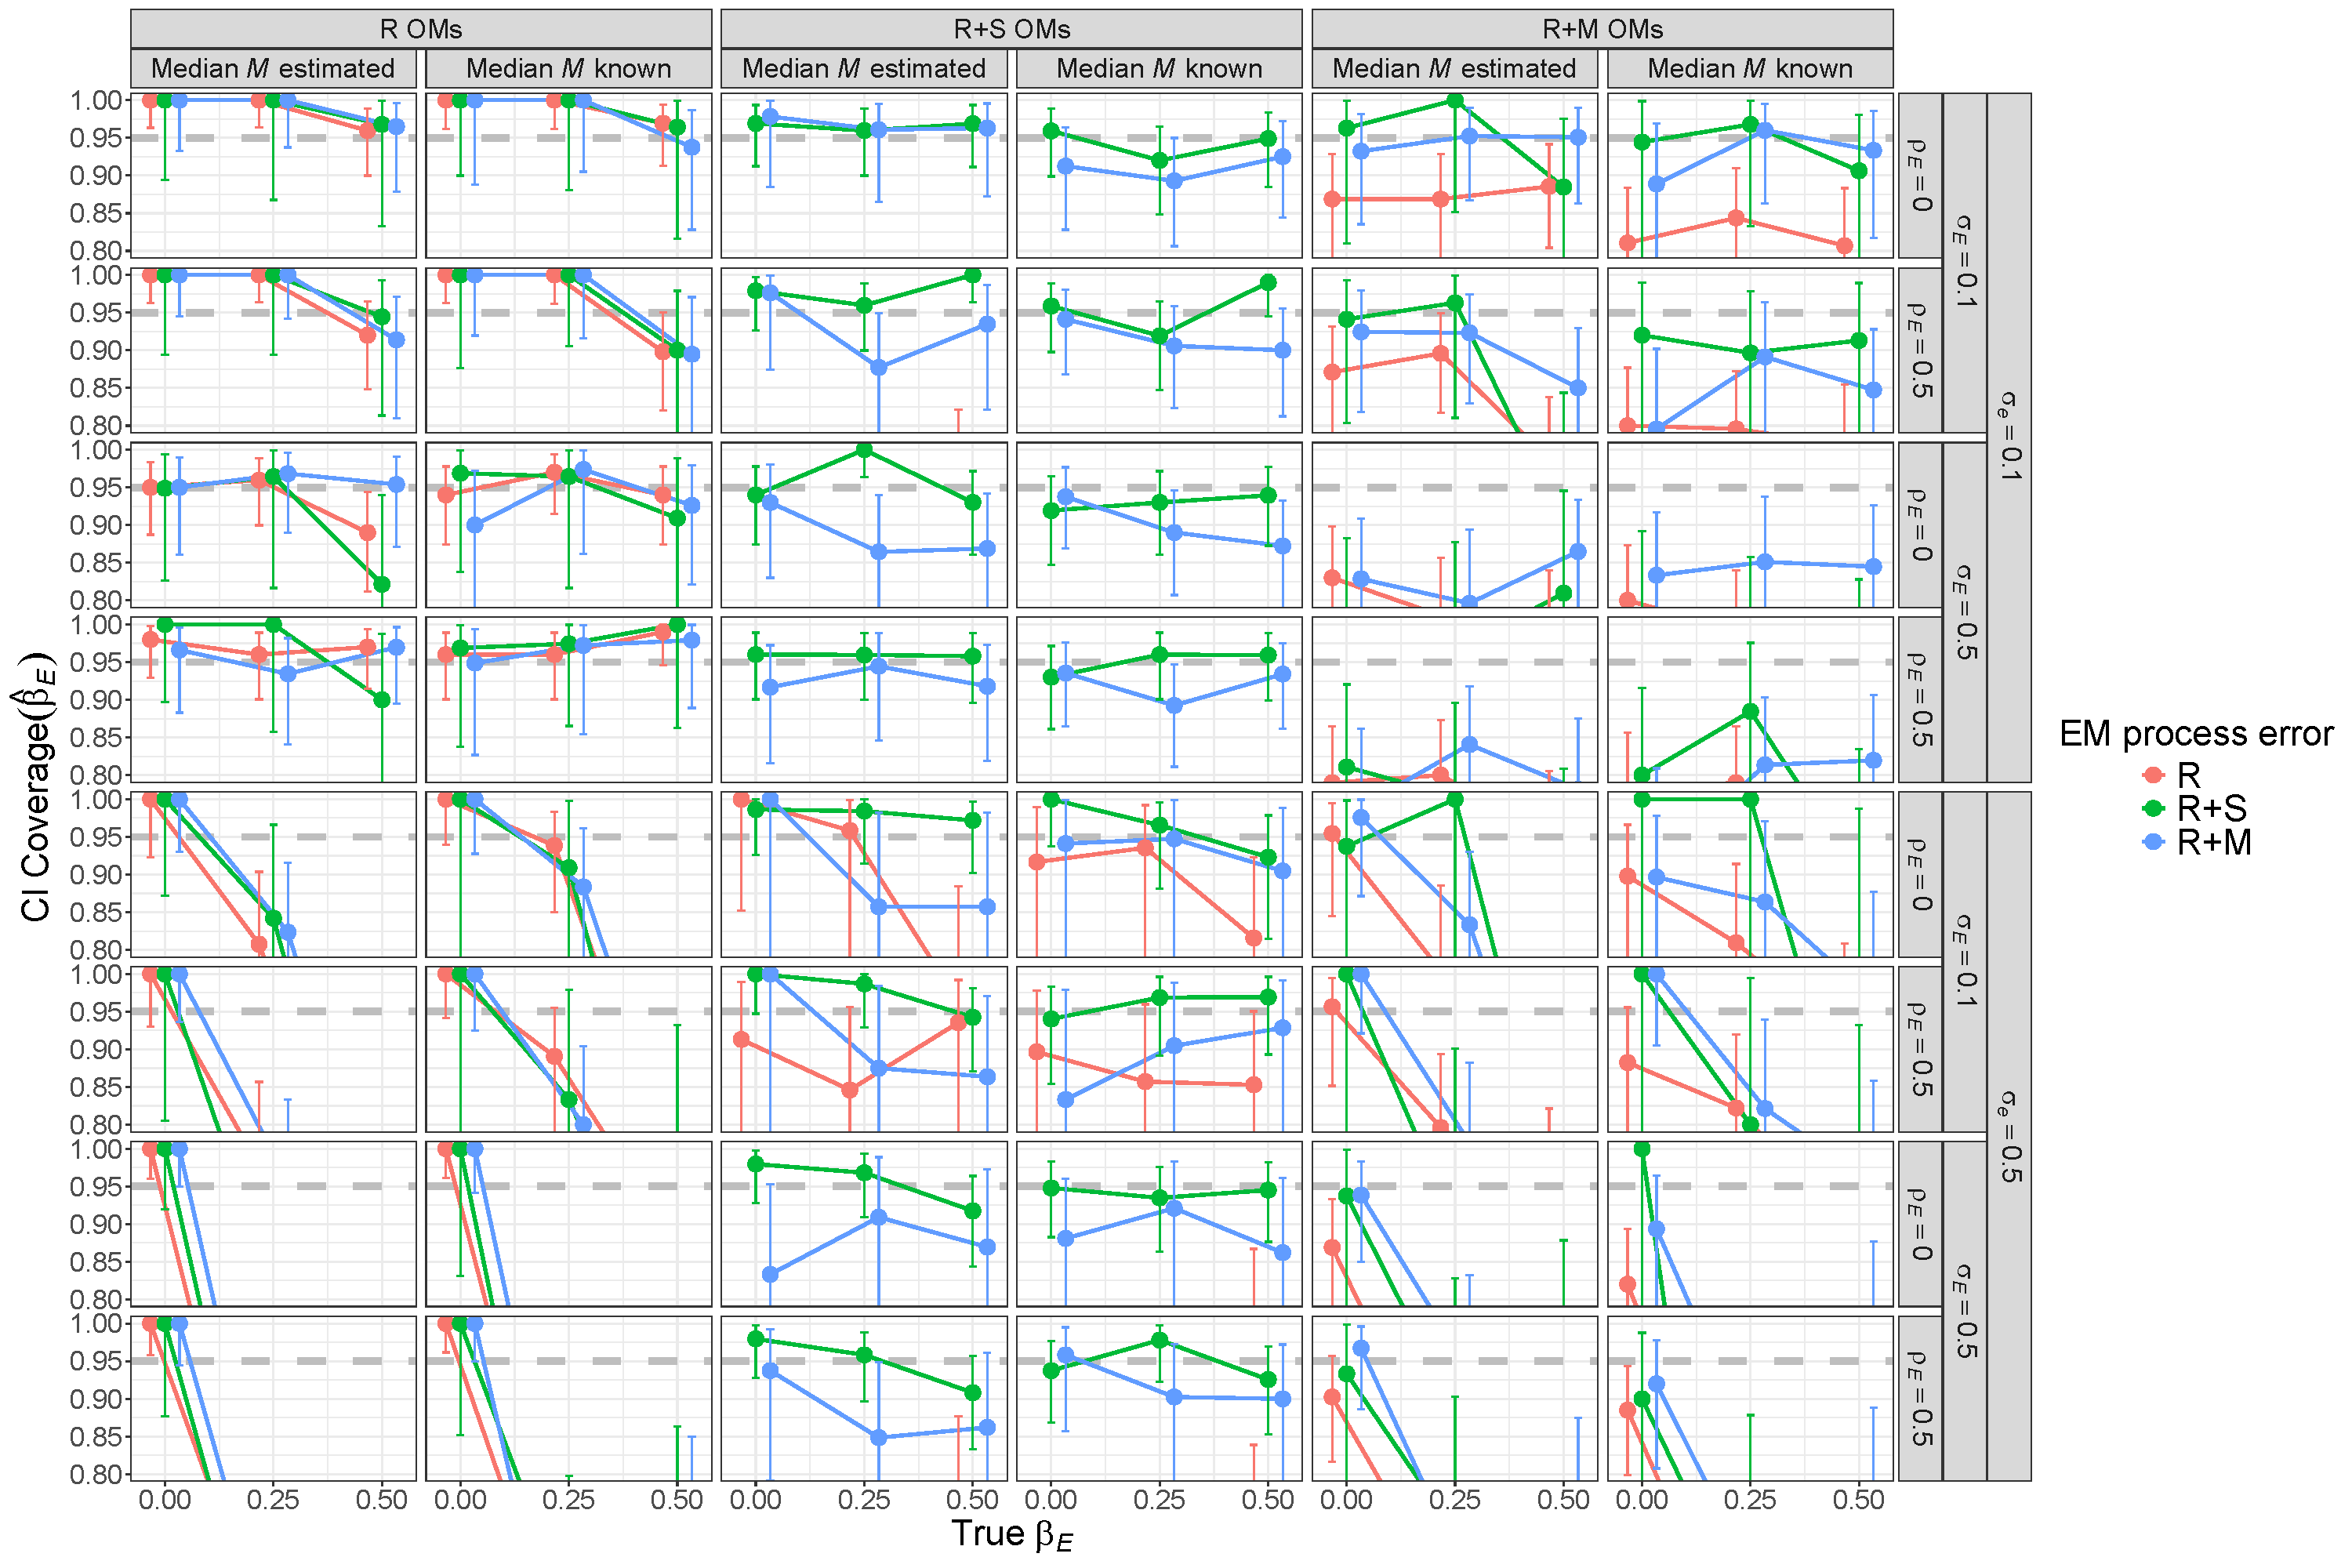
\includegraphics[height = \textheight]{beta_E_CI_coverage_main}
%DIFDELCMD < %%%
\DIFdelendFL \DIFaddbeginFL 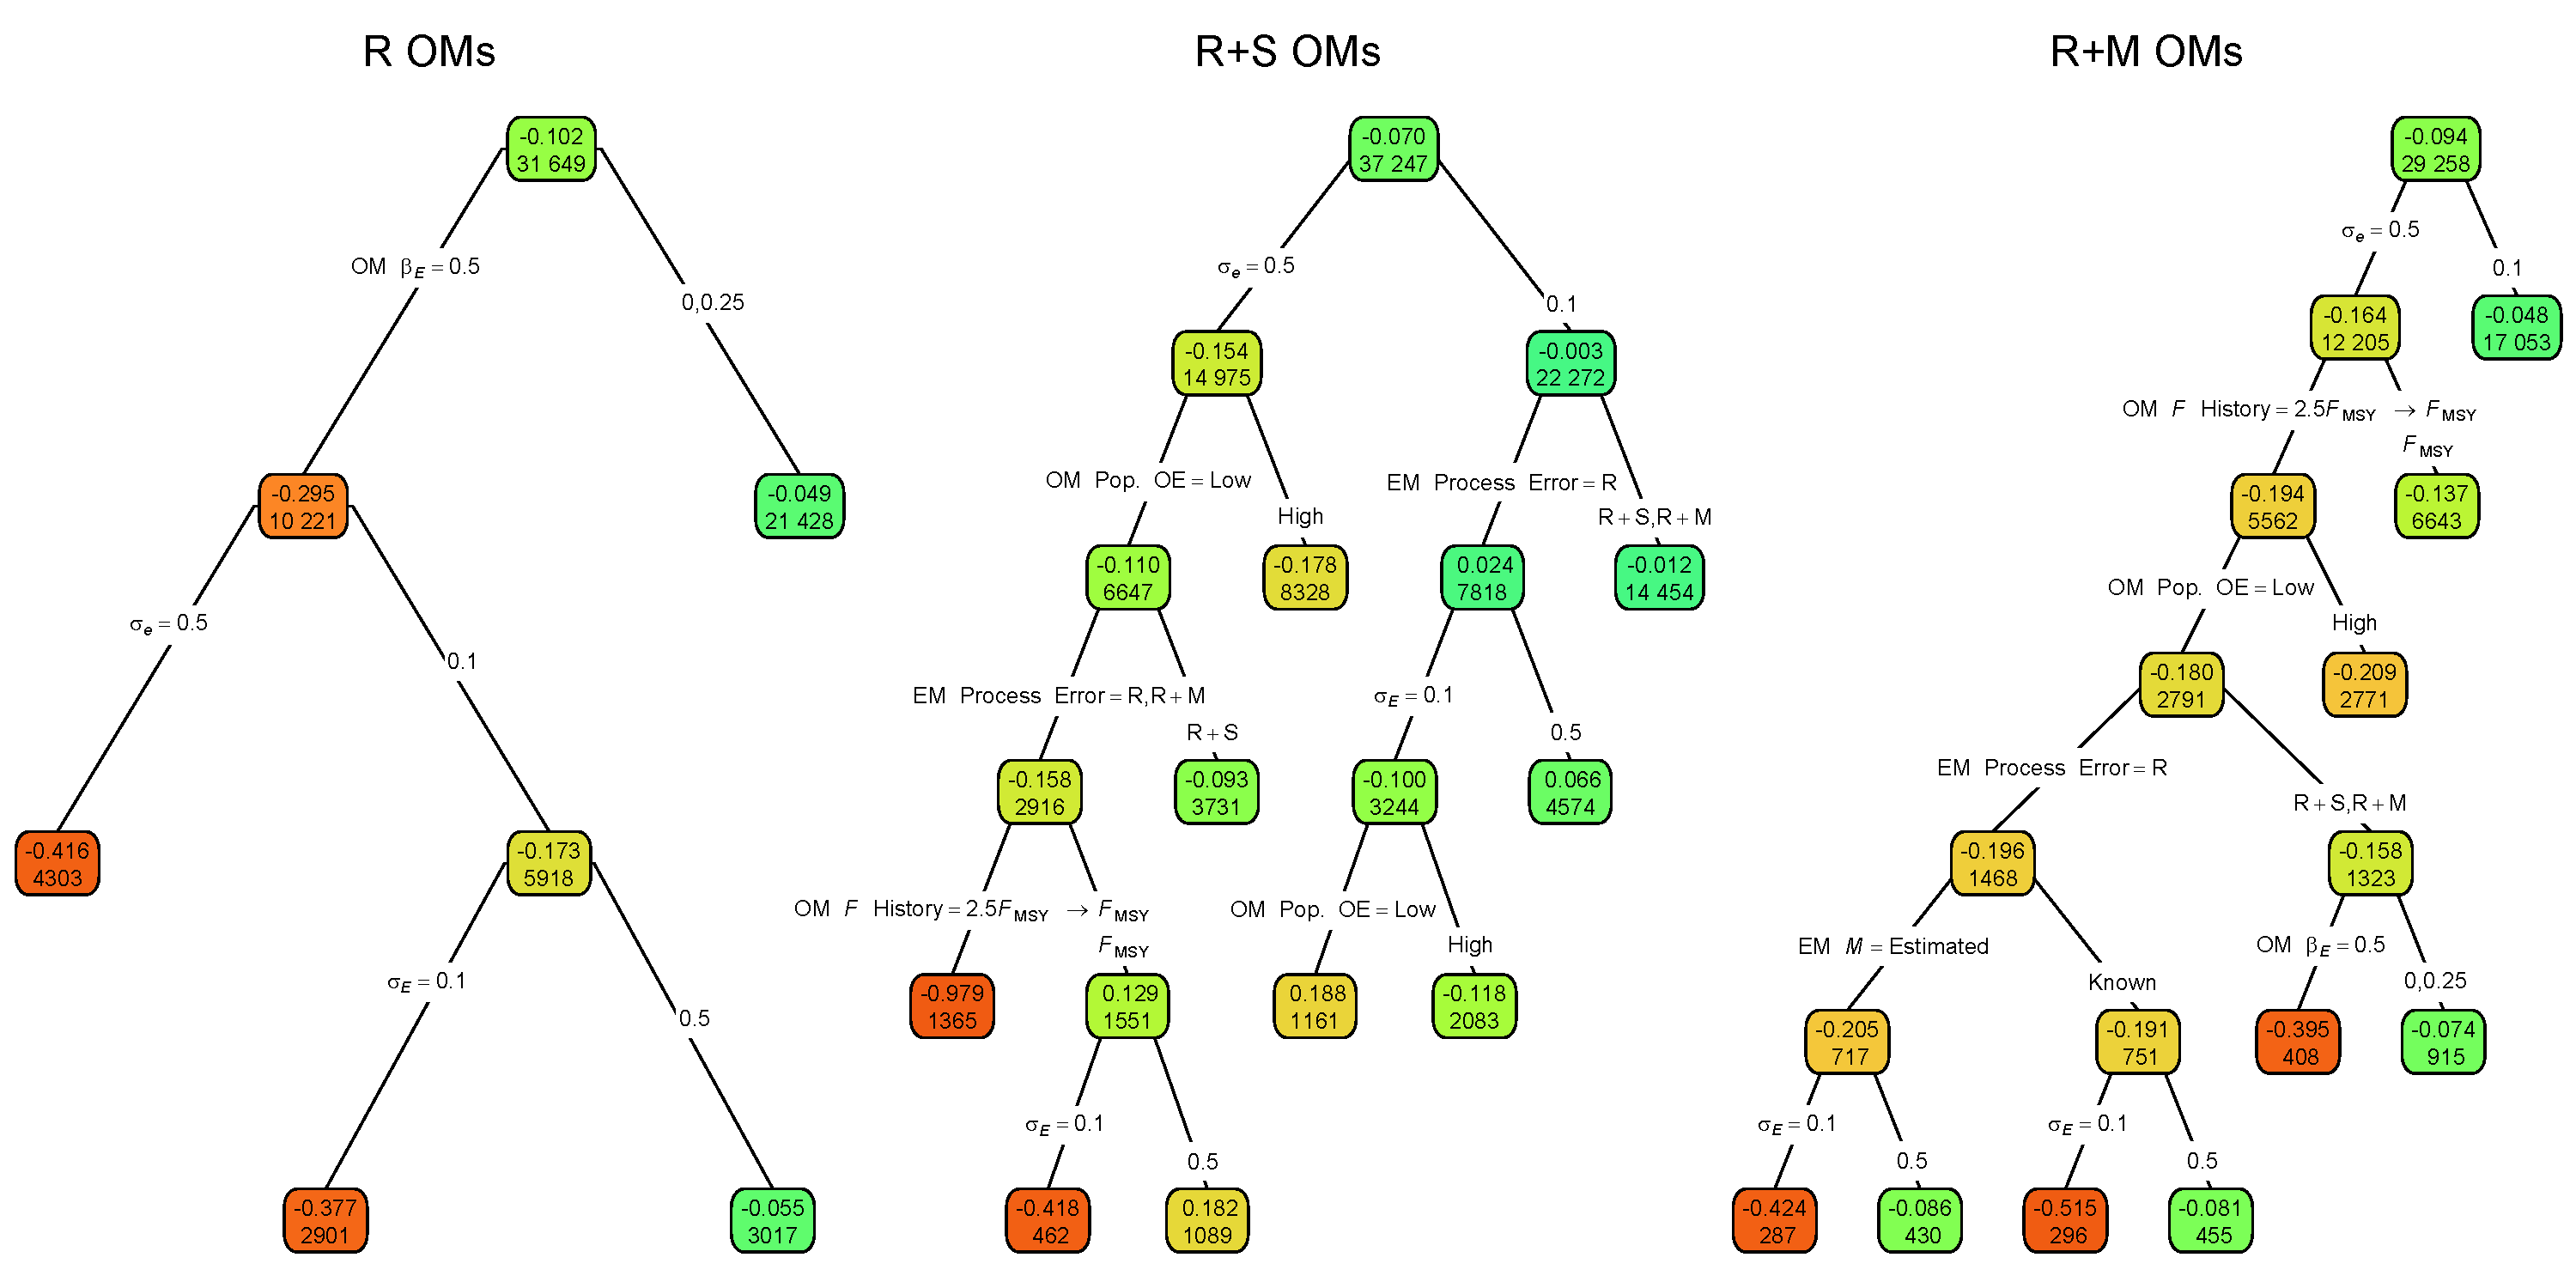
\includegraphics[width = 1.4\textwidth]{ecov_beta_bias_regtree_plots}
\DIFaddendFL \end{center}
\caption{\DIFdelbeginFL \DIFdelFL{Probability }\DIFdelendFL \DIFaddbeginFL \DIFaddFL{Regression trees indicating primary factors determining reductions in sums }\DIFaddendFL of \DIFdelbeginFL \DIFdelFL{95\% confidence interval for $\beta_E$ containing }\DIFdelendFL \DIFaddbeginFL \DIFaddFL{squares of errors in estimation of }\DIFaddendFL the \DIFdelbeginFL \DIFdelFL{true value }\DIFdelendFL \DIFaddbeginFL \DIFaddFL{covariate effect on $M$ }\DIFaddendFL for \DIFdelbeginFL \DIFdelFL{EMs }\DIFdelendFL \DIFaddbeginFL \DIFaddFL{operating models (OMs) }\DIFaddendFL with \DIFdelbeginFL \DIFdelFL{alternative }\DIFdelendFL process error \DIFdelbeginFL \DIFdelFL{assumptions }\DIFdelendFL \DIFaddbeginFL \DIFaddFL{on recruitment only (R), recruitment }\DIFaddendFL and \DIFdelbeginFL \DIFdelFL{treatment of median }\DIFdelendFL \DIFaddbeginFL \DIFaddFL{apparent survival (R+S), or recruitment and }\DIFaddendFL natural mortality (\DIFdelbeginFL \DIFdelFL{$\beta_M$ known or estimated}\DIFdelendFL \DIFaddbeginFL \DIFaddFL{R+M}\DIFaddendFL ). \DIFdelbeginFL \DIFdelFL{All OMs had low observation }\DIFdelendFL \DIFaddbeginFL \DIFaddFL{Each node shows the median }\DIFaddendFL error \DIFaddbeginFL \DIFaddFL{(top) }\DIFaddendFL and \DIFdelbeginFL \DIFdelFL{contrast in fishing mortality}\DIFdelendFL \DIFaddbeginFL \DIFaddFL{number of observations (bottom) for the corresponding subset}\DIFaddendFL . \DIFdelbeginFL \DIFdelFL{Vertical lines represent 95\% confidence intervals}\DIFdelendFL \DIFaddbeginFL \DIFaddFL{Lower or higher median absolute errors of the process error assumption are indicated by more green or red polygons, respectively}\DIFaddendFL . \DIFaddbeginFL \DIFaddFL{See Table \ref{factor_table} for description of OM and EM factors defining nodes and branches.}\DIFaddendFL }\DIFdelbeginFL %DIFDELCMD < \label{beta_E_CI_coverage}
%DIFDELCMD < %%%
\DIFdelendFL \DIFaddbeginFL \label{ecov_effect_bias_regtree}
\DIFaddendFL \end{figure}
\end{landscape}

\begin{landscape}
\begin{figure}
\begin{center}
\DIFdelbeginFL %DIFDELCMD < 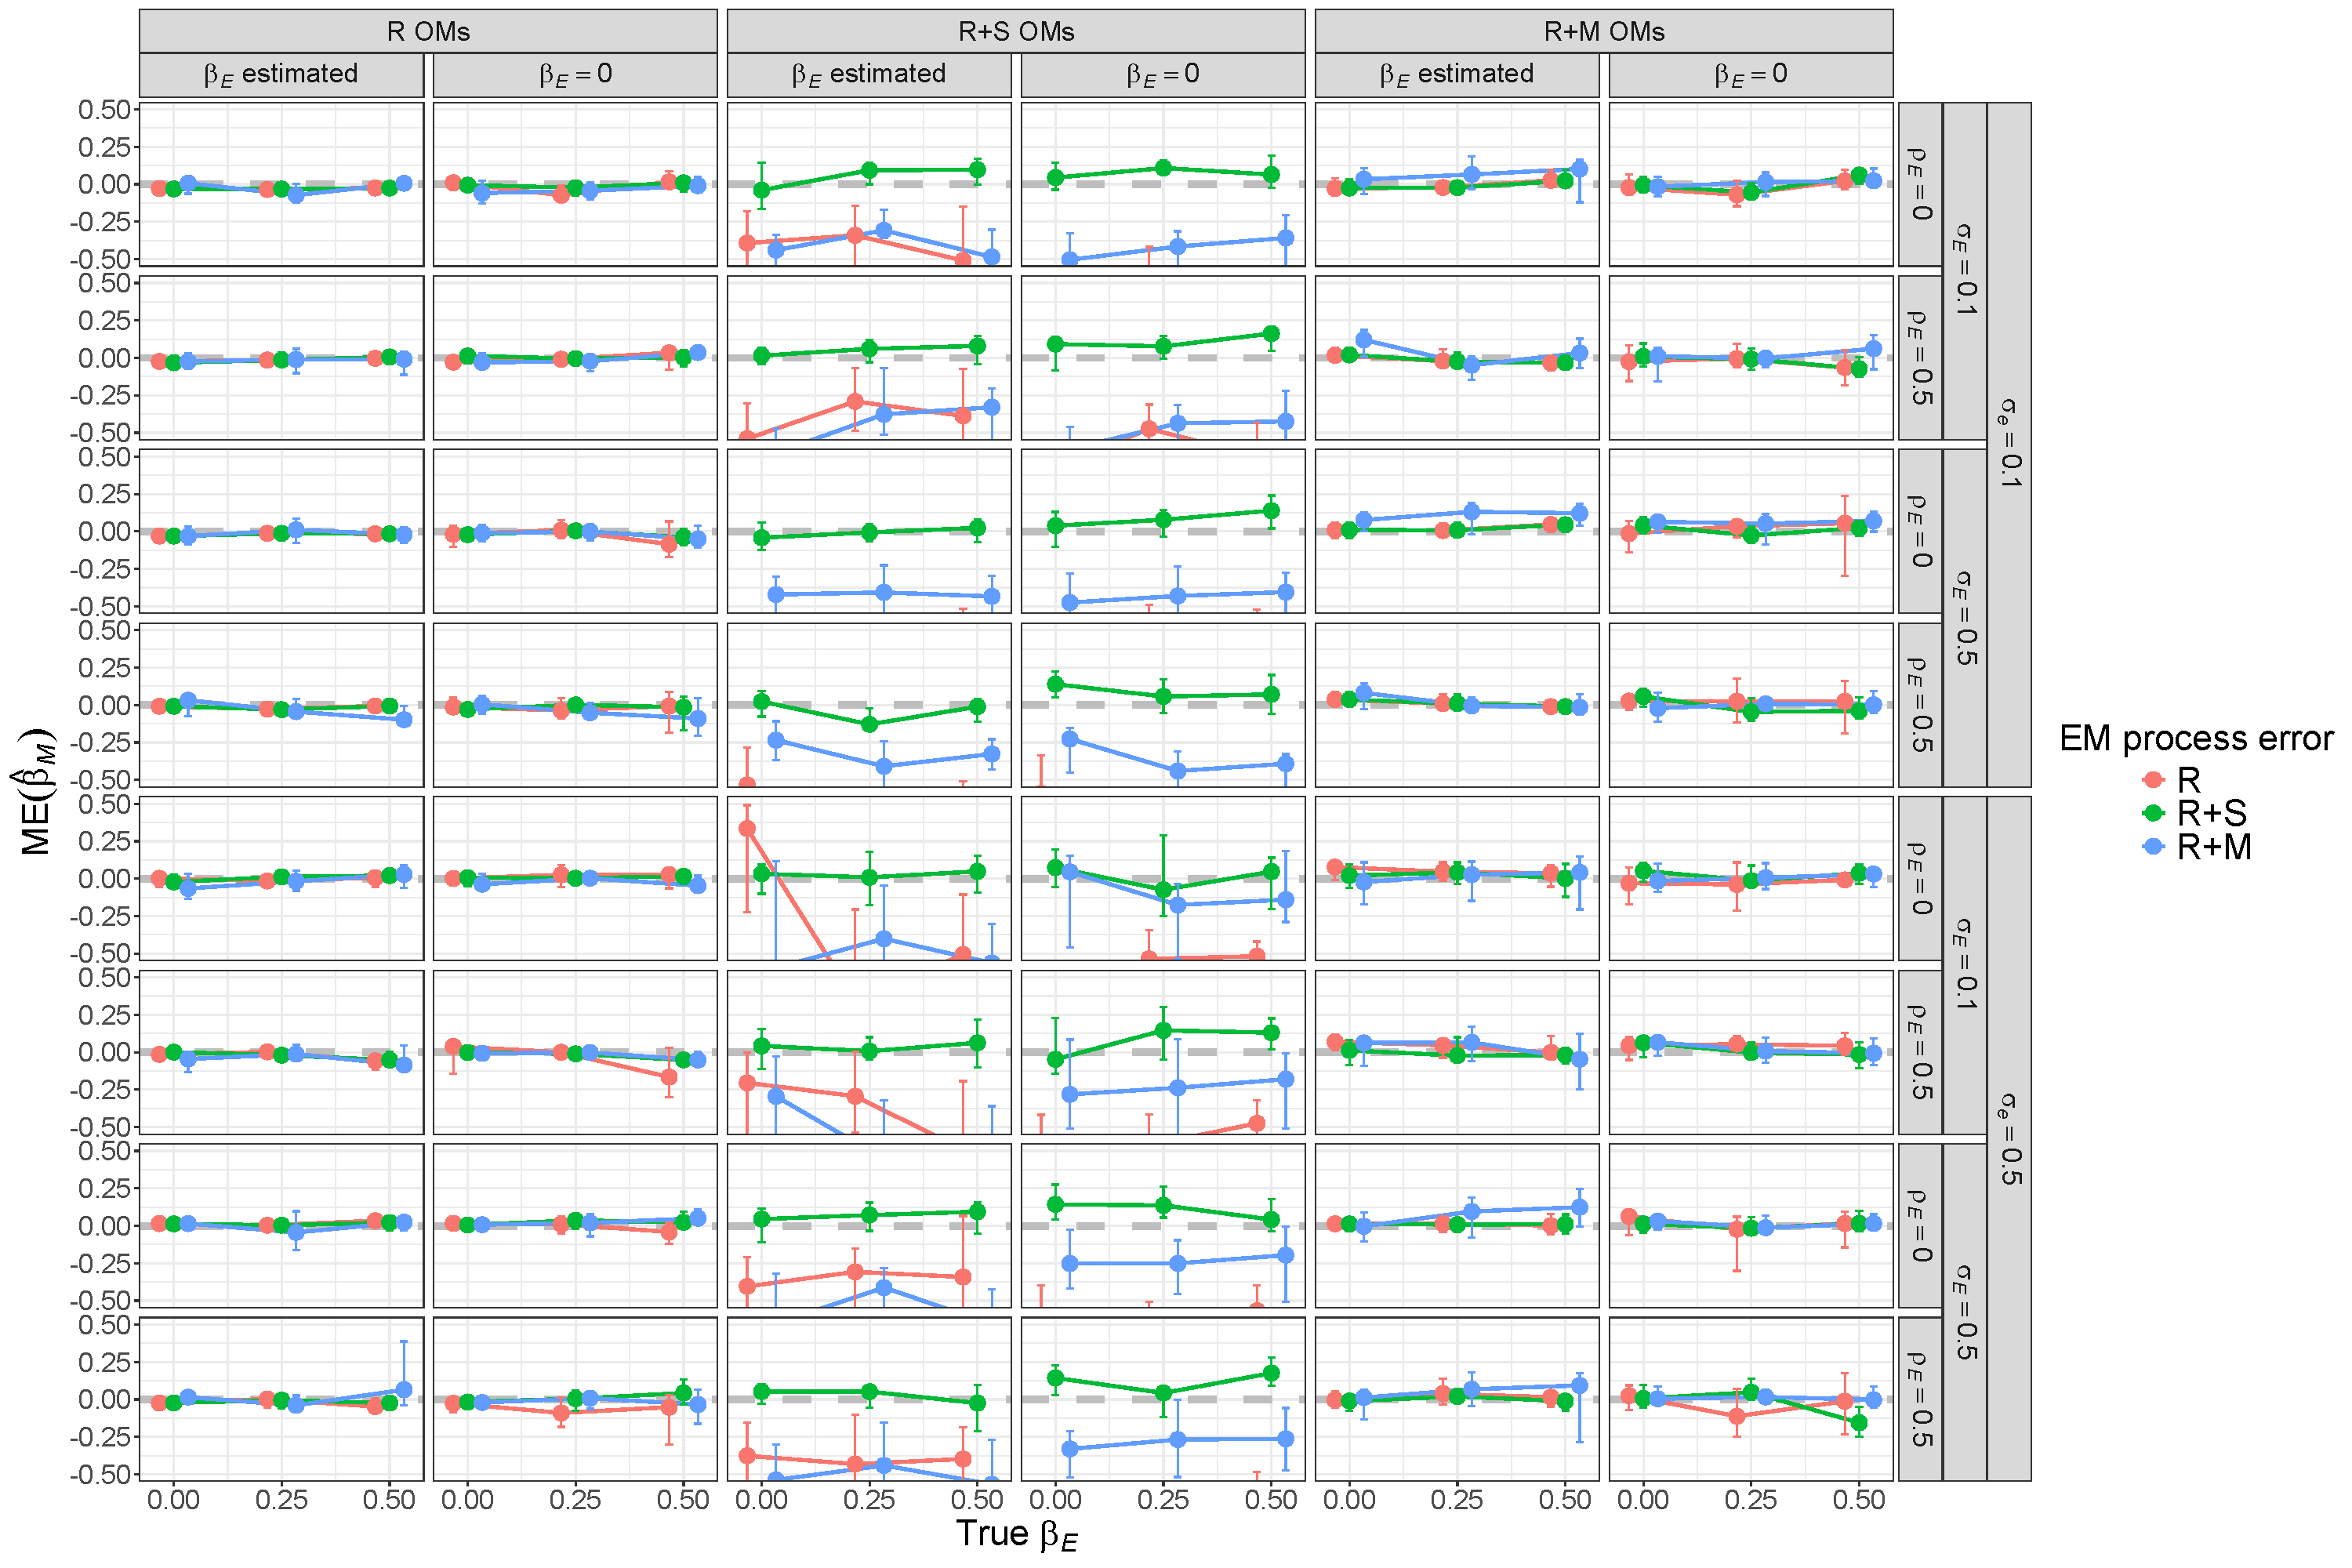
\includegraphics[height = \textheight]{beta_M_bias_main}
%DIFDELCMD < %%%
\DIFdelendFL \DIFaddbeginFL 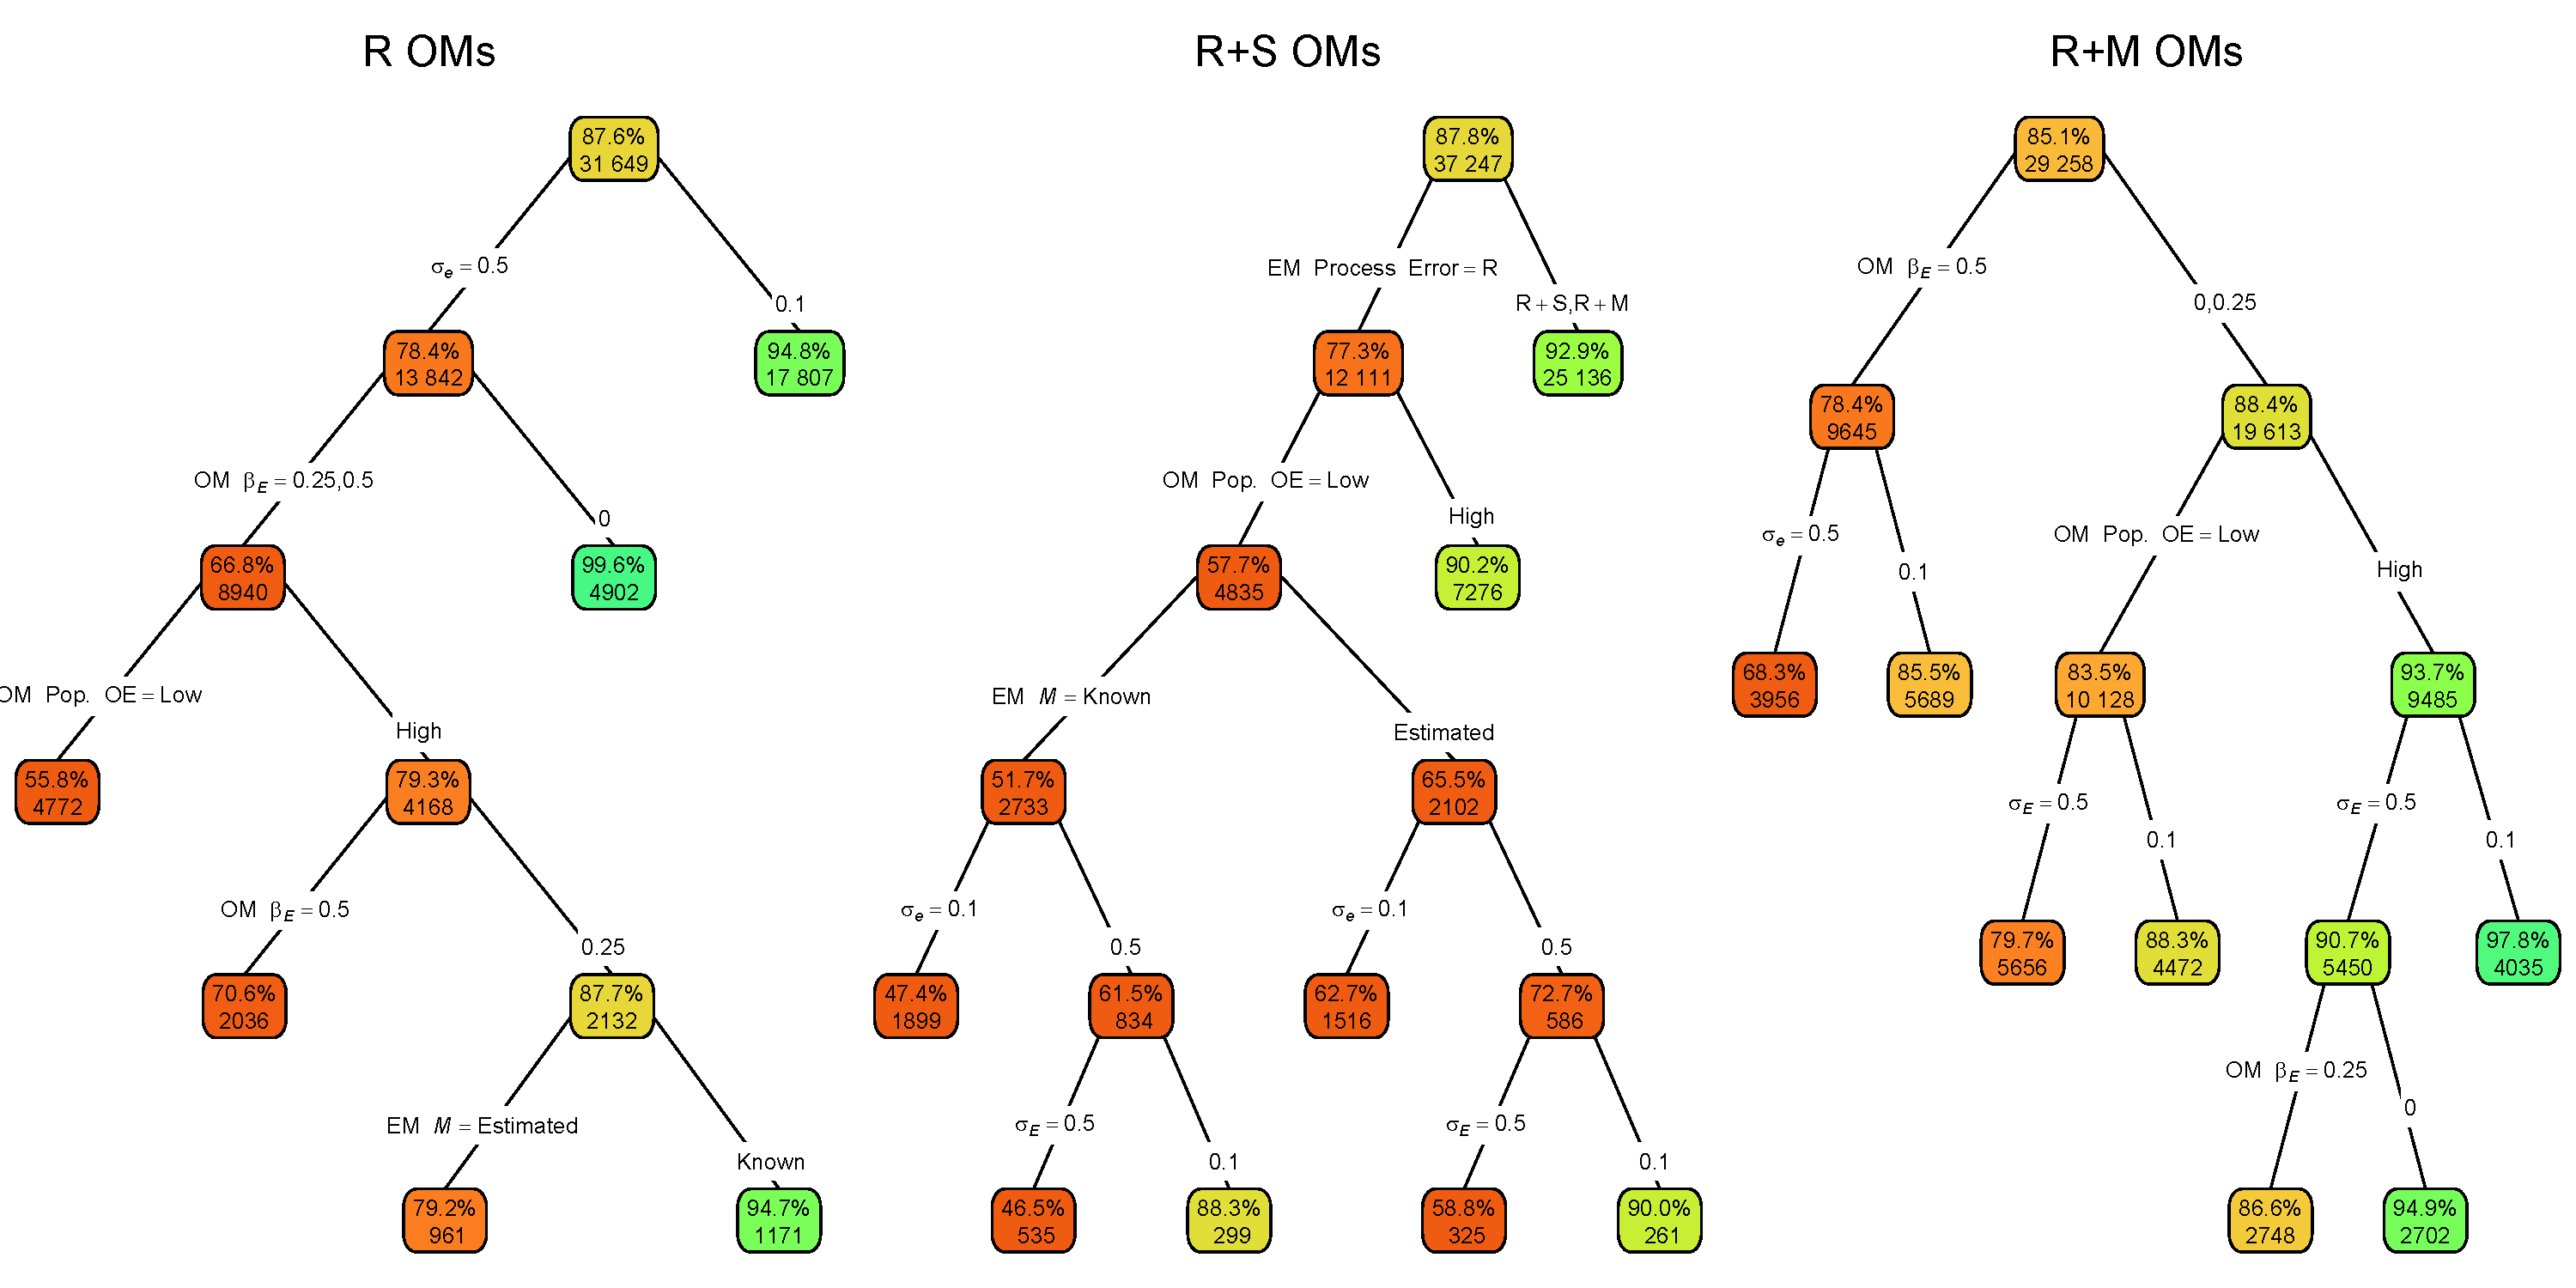
\includegraphics[width = 1.4\textwidth]{ecov_beta_CI_coverage_regtree_plots}
\DIFaddendFL \end{center}
\caption{\DIFdelbeginFL \DIFdelFL{Median error }\DIFdelendFL \DIFaddbeginFL \DIFaddFL{Classification trees indicating primary factors determining whether confidence intervals for estimated covariate effects on $M$ in estimating models }\DIFaddendFL (\DIFdelbeginFL \DIFdelFL{ME) of estimates of $\beta_M$ from fitting }\DIFdelendFL EMs\DIFaddbeginFL \DIFaddFL{) fitted to operating models (OMs) }\DIFaddendFL with \DIFdelbeginFL \DIFdelFL{alternative }\DIFdelendFL process error \DIFdelbeginFL \DIFdelFL{assumptions }\DIFdelendFL \DIFaddbeginFL \DIFaddFL{on recruitment only (R), recruitment }\DIFaddendFL and \DIFdelbeginFL \DIFdelFL{treatment of covariate effect }\DIFdelendFL \DIFaddbeginFL \DIFaddFL{apparent survival }\DIFaddendFL (\DIFdelbeginFL \DIFdelFL{$\beta_E = 0$ }\DIFdelendFL \DIFaddbeginFL \DIFaddFL{R+S), }\DIFaddendFL or \DIFdelbeginFL \DIFdelFL{estimated}\DIFdelendFL \DIFaddbeginFL \DIFaddFL{recruitment and natural mortality (R+M}\DIFaddendFL ) \DIFaddbeginFL \DIFaddFL{included the true value}\DIFaddendFL . \DIFdelbeginFL \DIFdelFL{All OMs had low observation }\DIFdelendFL \DIFaddbeginFL \DIFaddFL{Each node shows the median }\DIFaddendFL error \DIFaddbeginFL \DIFaddFL{(top) }\DIFaddendFL and \DIFdelbeginFL \DIFdelFL{contrast in fishing mortality}\DIFdelendFL \DIFaddbeginFL \DIFaddFL{number of observations (bottom) for the corresponding subset}\DIFaddendFL . \DIFdelbeginFL \DIFdelFL{Vertical lines represent 95\% confidence intervals}\DIFdelendFL \DIFaddbeginFL \DIFaddFL{Lower or higher median absolute errors of the process error assumption are indicated by more green or red polygons, respectively}\DIFaddendFL . \DIFaddbeginFL \DIFaddFL{See Table \ref{factor_table} for description of OM and EM factors defining nodes and branches.}\DIFaddendFL }\DIFdelbeginFL %DIFDELCMD < \label{beta_M_bias}
%DIFDELCMD < %%%
\DIFdelendFL \DIFaddbeginFL \label{ecov_effect_CI_coverage_regtree}
\DIFaddendFL \end{figure}
\end{landscape}

\begin{landscape}
\begin{figure}
\begin{center}
\DIFdelbeginFL %DIFDELCMD < 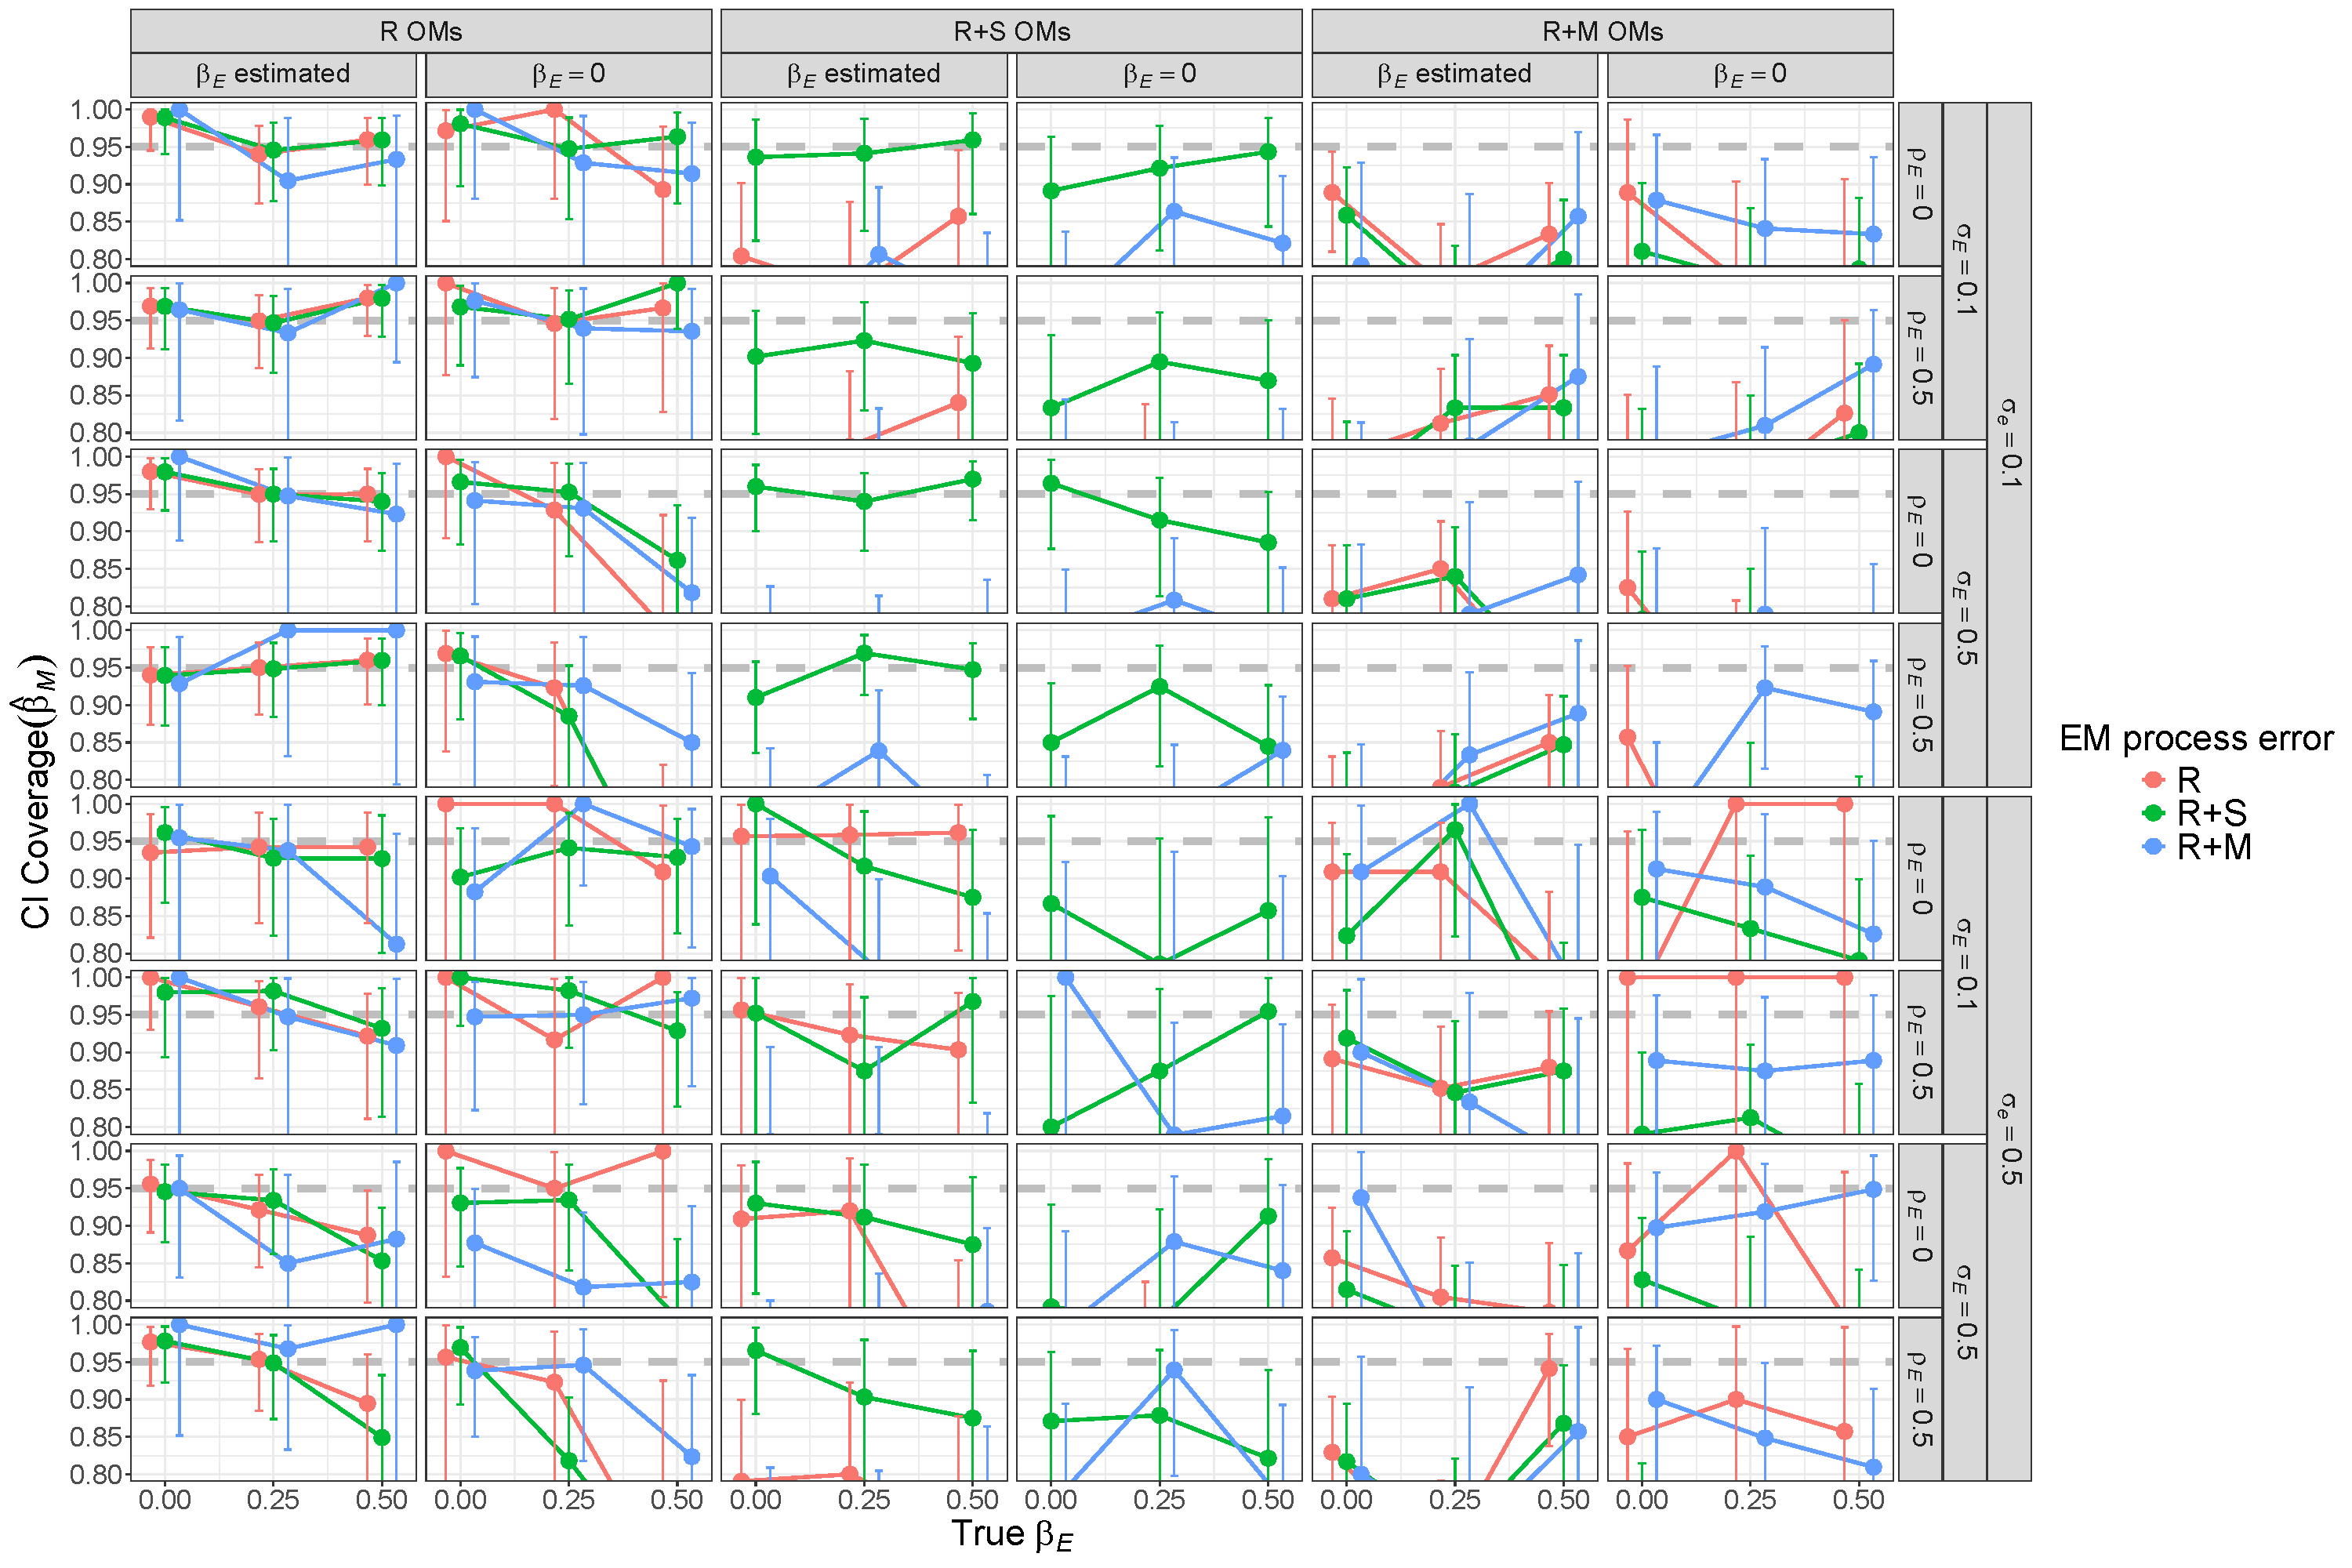
\includegraphics[height = \textheight]{beta_M_CI_coverage_main}
%DIFDELCMD < %%%
\DIFdelendFL \DIFaddbeginFL 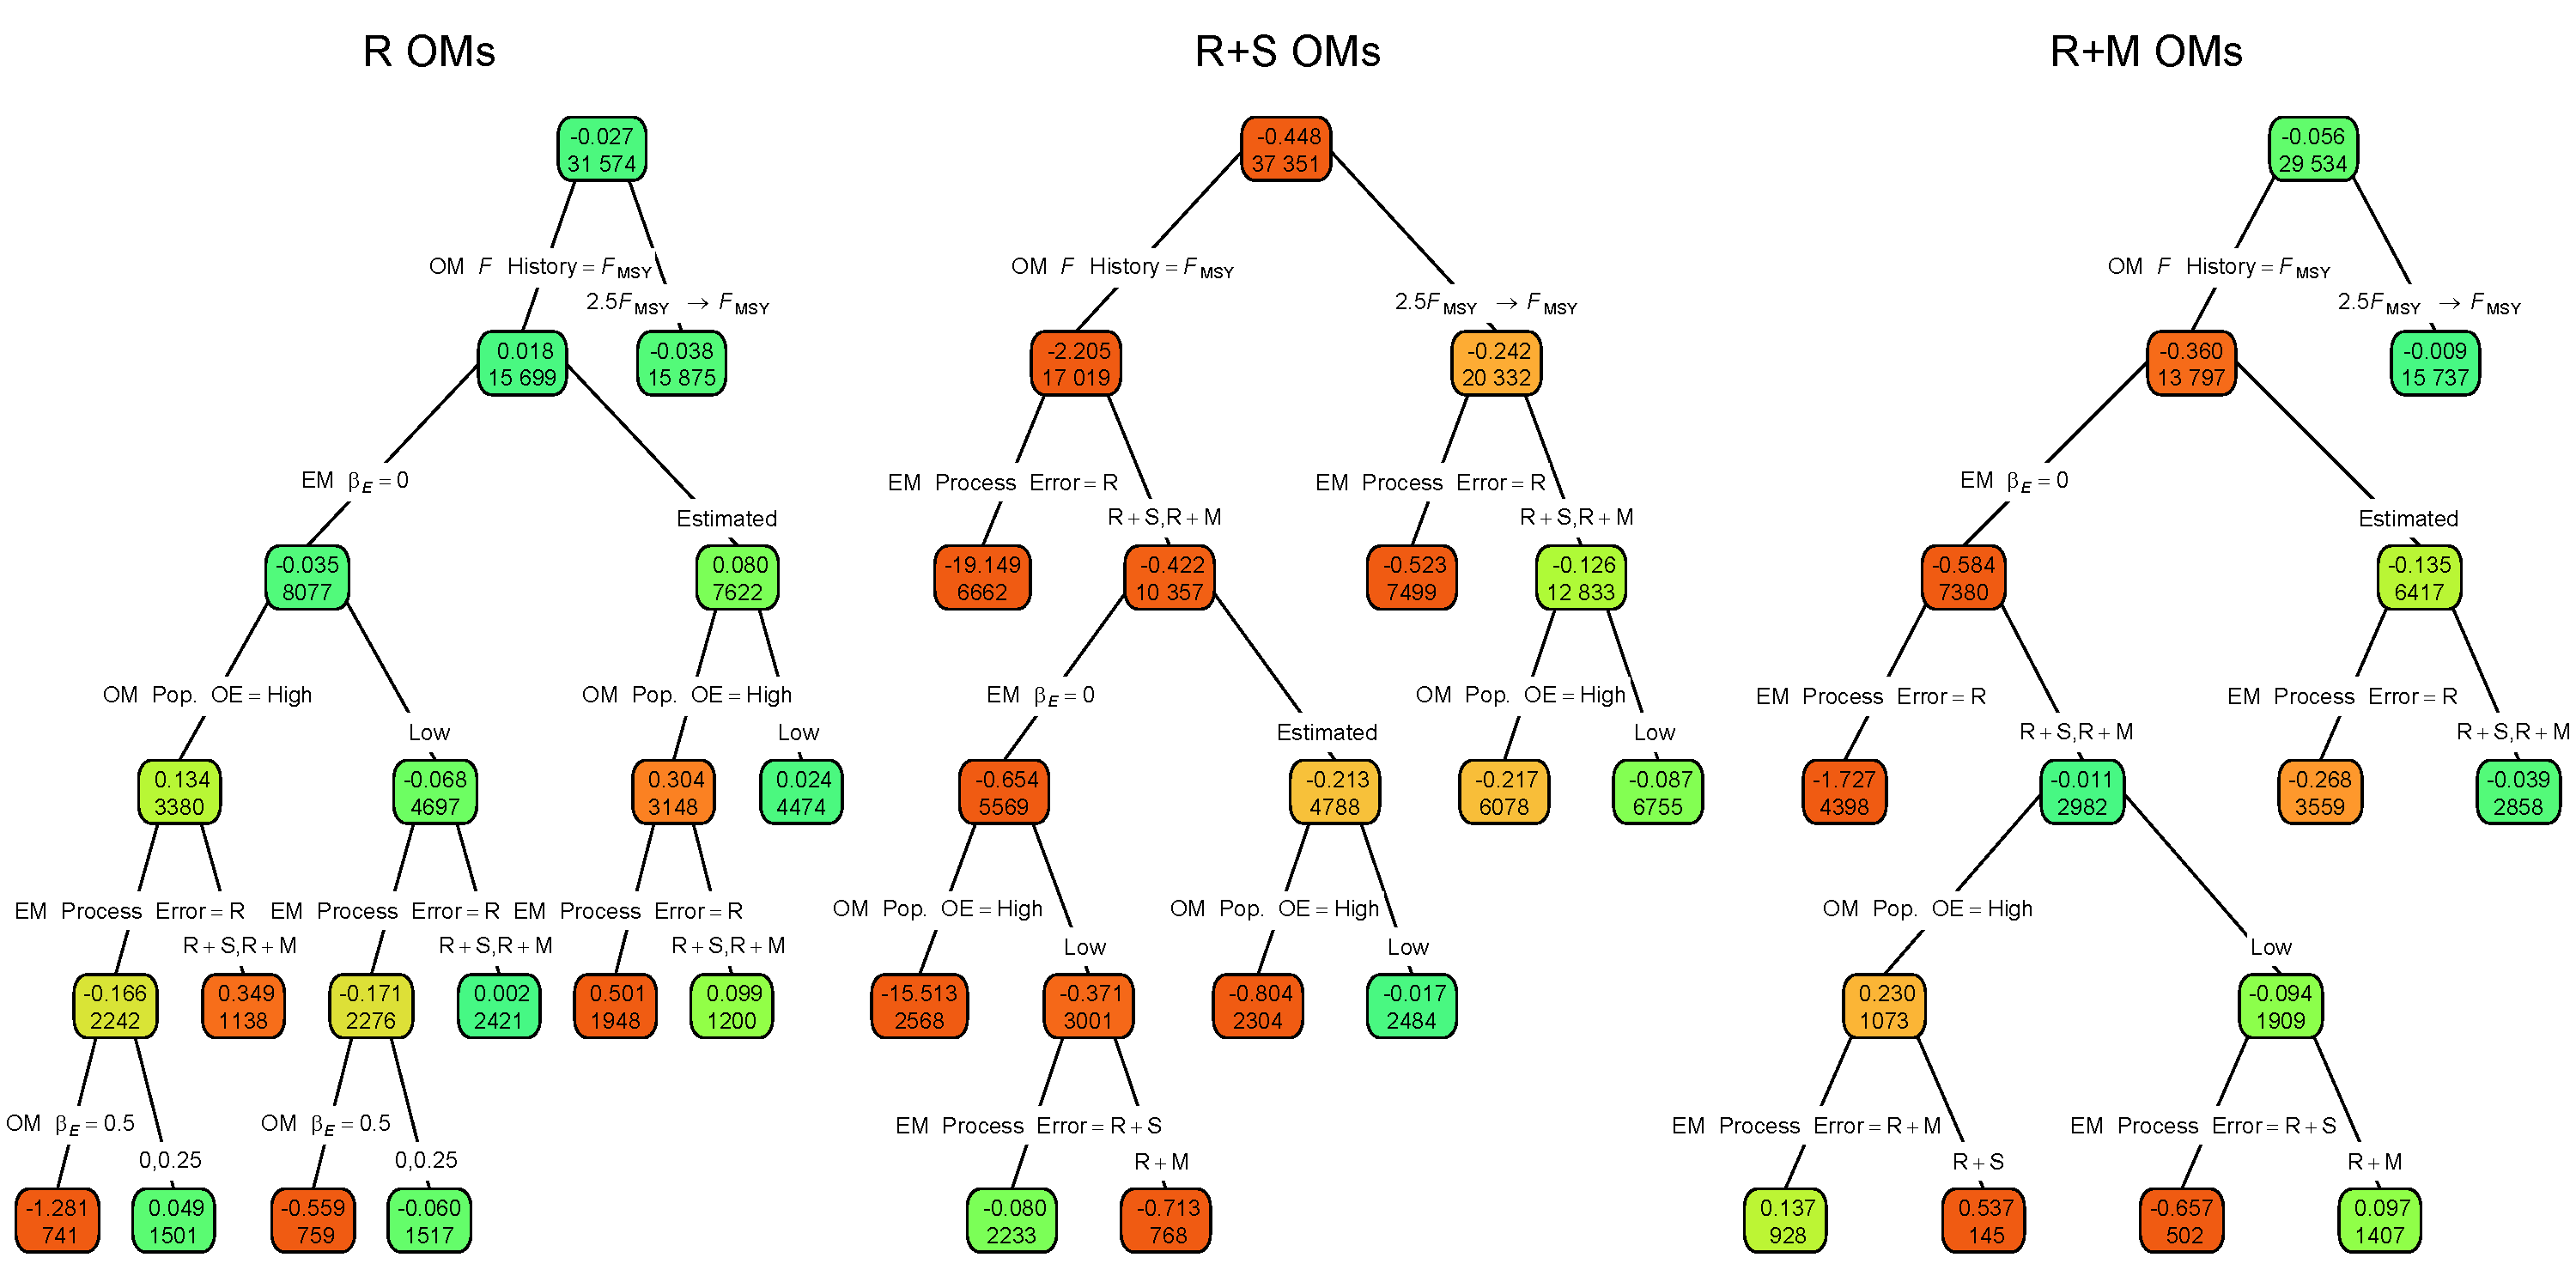
\includegraphics[width = 1.4\textwidth]{median_M_bias_regtree_plots}
\DIFaddendFL \end{center}
\caption{\DIFdelbeginFL \DIFdelFL{Probability }\DIFdelendFL \DIFaddbeginFL \DIFaddFL{Regression trees indicating primary factors determining reductions in sums }\DIFaddendFL of \DIFdelbeginFL \DIFdelFL{95\% confidence interval for $\beta_M$ containing }\DIFdelendFL \DIFaddbeginFL \DIFaddFL{squares of errors in estimation of }\DIFaddendFL the \DIFdelbeginFL \DIFdelFL{true value for }\DIFdelendFL \DIFaddbeginFL \DIFaddFL{median $M$ parameter ($\beta_M$) in estimating models (}\DIFaddendFL EMs\DIFaddbeginFL \DIFaddFL{) fitted to operating models (OMs) }\DIFaddendFL with \DIFdelbeginFL \DIFdelFL{alternative }\DIFdelendFL process error \DIFdelbeginFL \DIFdelFL{assumptions }\DIFdelendFL \DIFaddbeginFL \DIFaddFL{on recruitment only (R), recruitment }\DIFaddendFL and \DIFdelbeginFL \DIFdelFL{treatment of covariate effect }\DIFdelendFL \DIFaddbeginFL \DIFaddFL{apparent survival }\DIFaddendFL (\DIFdelbeginFL \DIFdelFL{$\beta_E = 0$ }\DIFdelendFL \DIFaddbeginFL \DIFaddFL{R+S), }\DIFaddendFL or \DIFdelbeginFL \DIFdelFL{estimated}\DIFdelendFL \DIFaddbeginFL \DIFaddFL{recruitment and natural mortality (R+M}\DIFaddendFL ). \DIFdelbeginFL \DIFdelFL{All OMs had low observation }\DIFdelendFL \DIFaddbeginFL \DIFaddFL{Each node shows the median }\DIFaddendFL error \DIFaddbeginFL \DIFaddFL{(top) }\DIFaddendFL and \DIFdelbeginFL \DIFdelFL{contrast in fishing mortality}\DIFdelendFL \DIFaddbeginFL \DIFaddFL{number of observations (bottom) for the corresponding subset}\DIFaddendFL . \DIFdelbeginFL \DIFdelFL{Vertical lines represent 95\% confidence intervals}\DIFdelendFL \DIFaddbeginFL \DIFaddFL{Lower or higher median absolute errors of the process error assumption are indicated by more green or red polygons, respectively}\DIFaddendFL . \DIFaddbeginFL \DIFaddFL{See Table \ref{factor_table} for description of OM and EM factors defining nodes and branches.}\DIFaddendFL }\DIFdelbeginFL %DIFDELCMD < \label{beta_M_CI_coverage}
%DIFDELCMD < %%%
\DIFdelendFL \DIFaddbeginFL \label{med_M_bias_regtree}
\DIFaddendFL \end{figure}
\end{landscape}

\begin{landscape}
\begin{figure}
\begin{center}
\DIFdelbeginFL %DIFDELCMD < 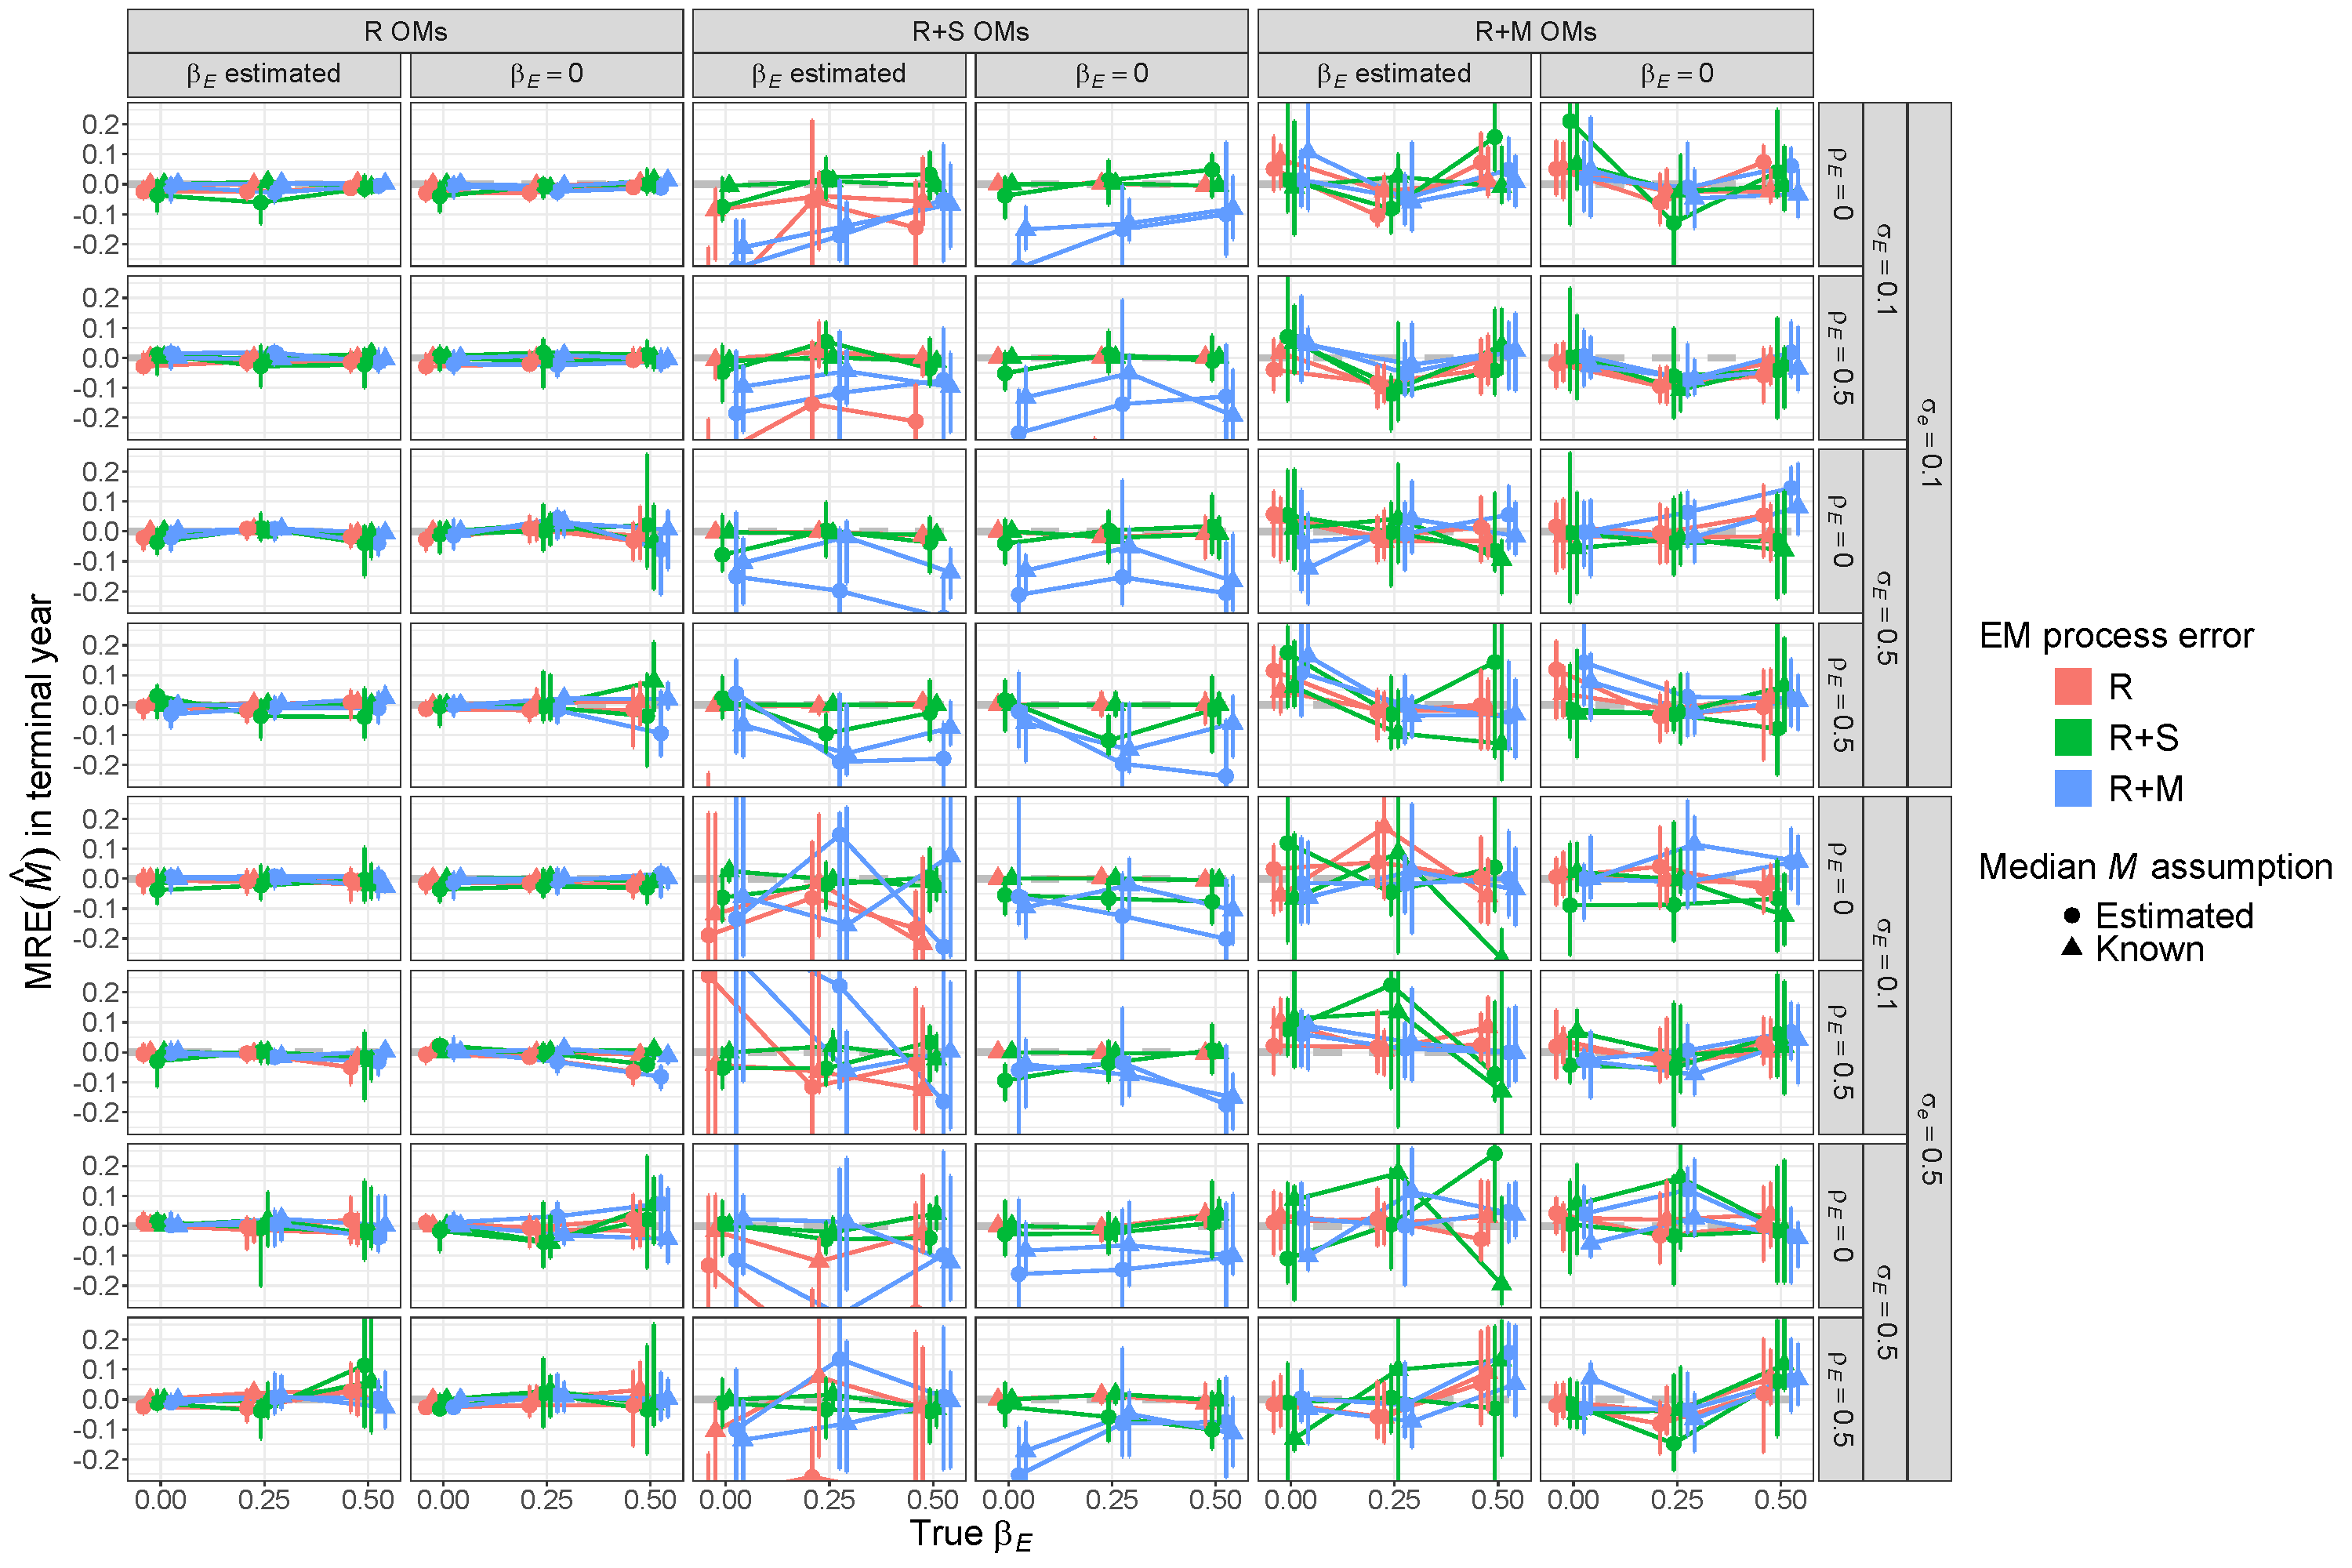
\includegraphics[height = \textheight]{terminal_year_M_bias_main}
%DIFDELCMD < %%%
\DIFdelendFL \DIFaddbeginFL 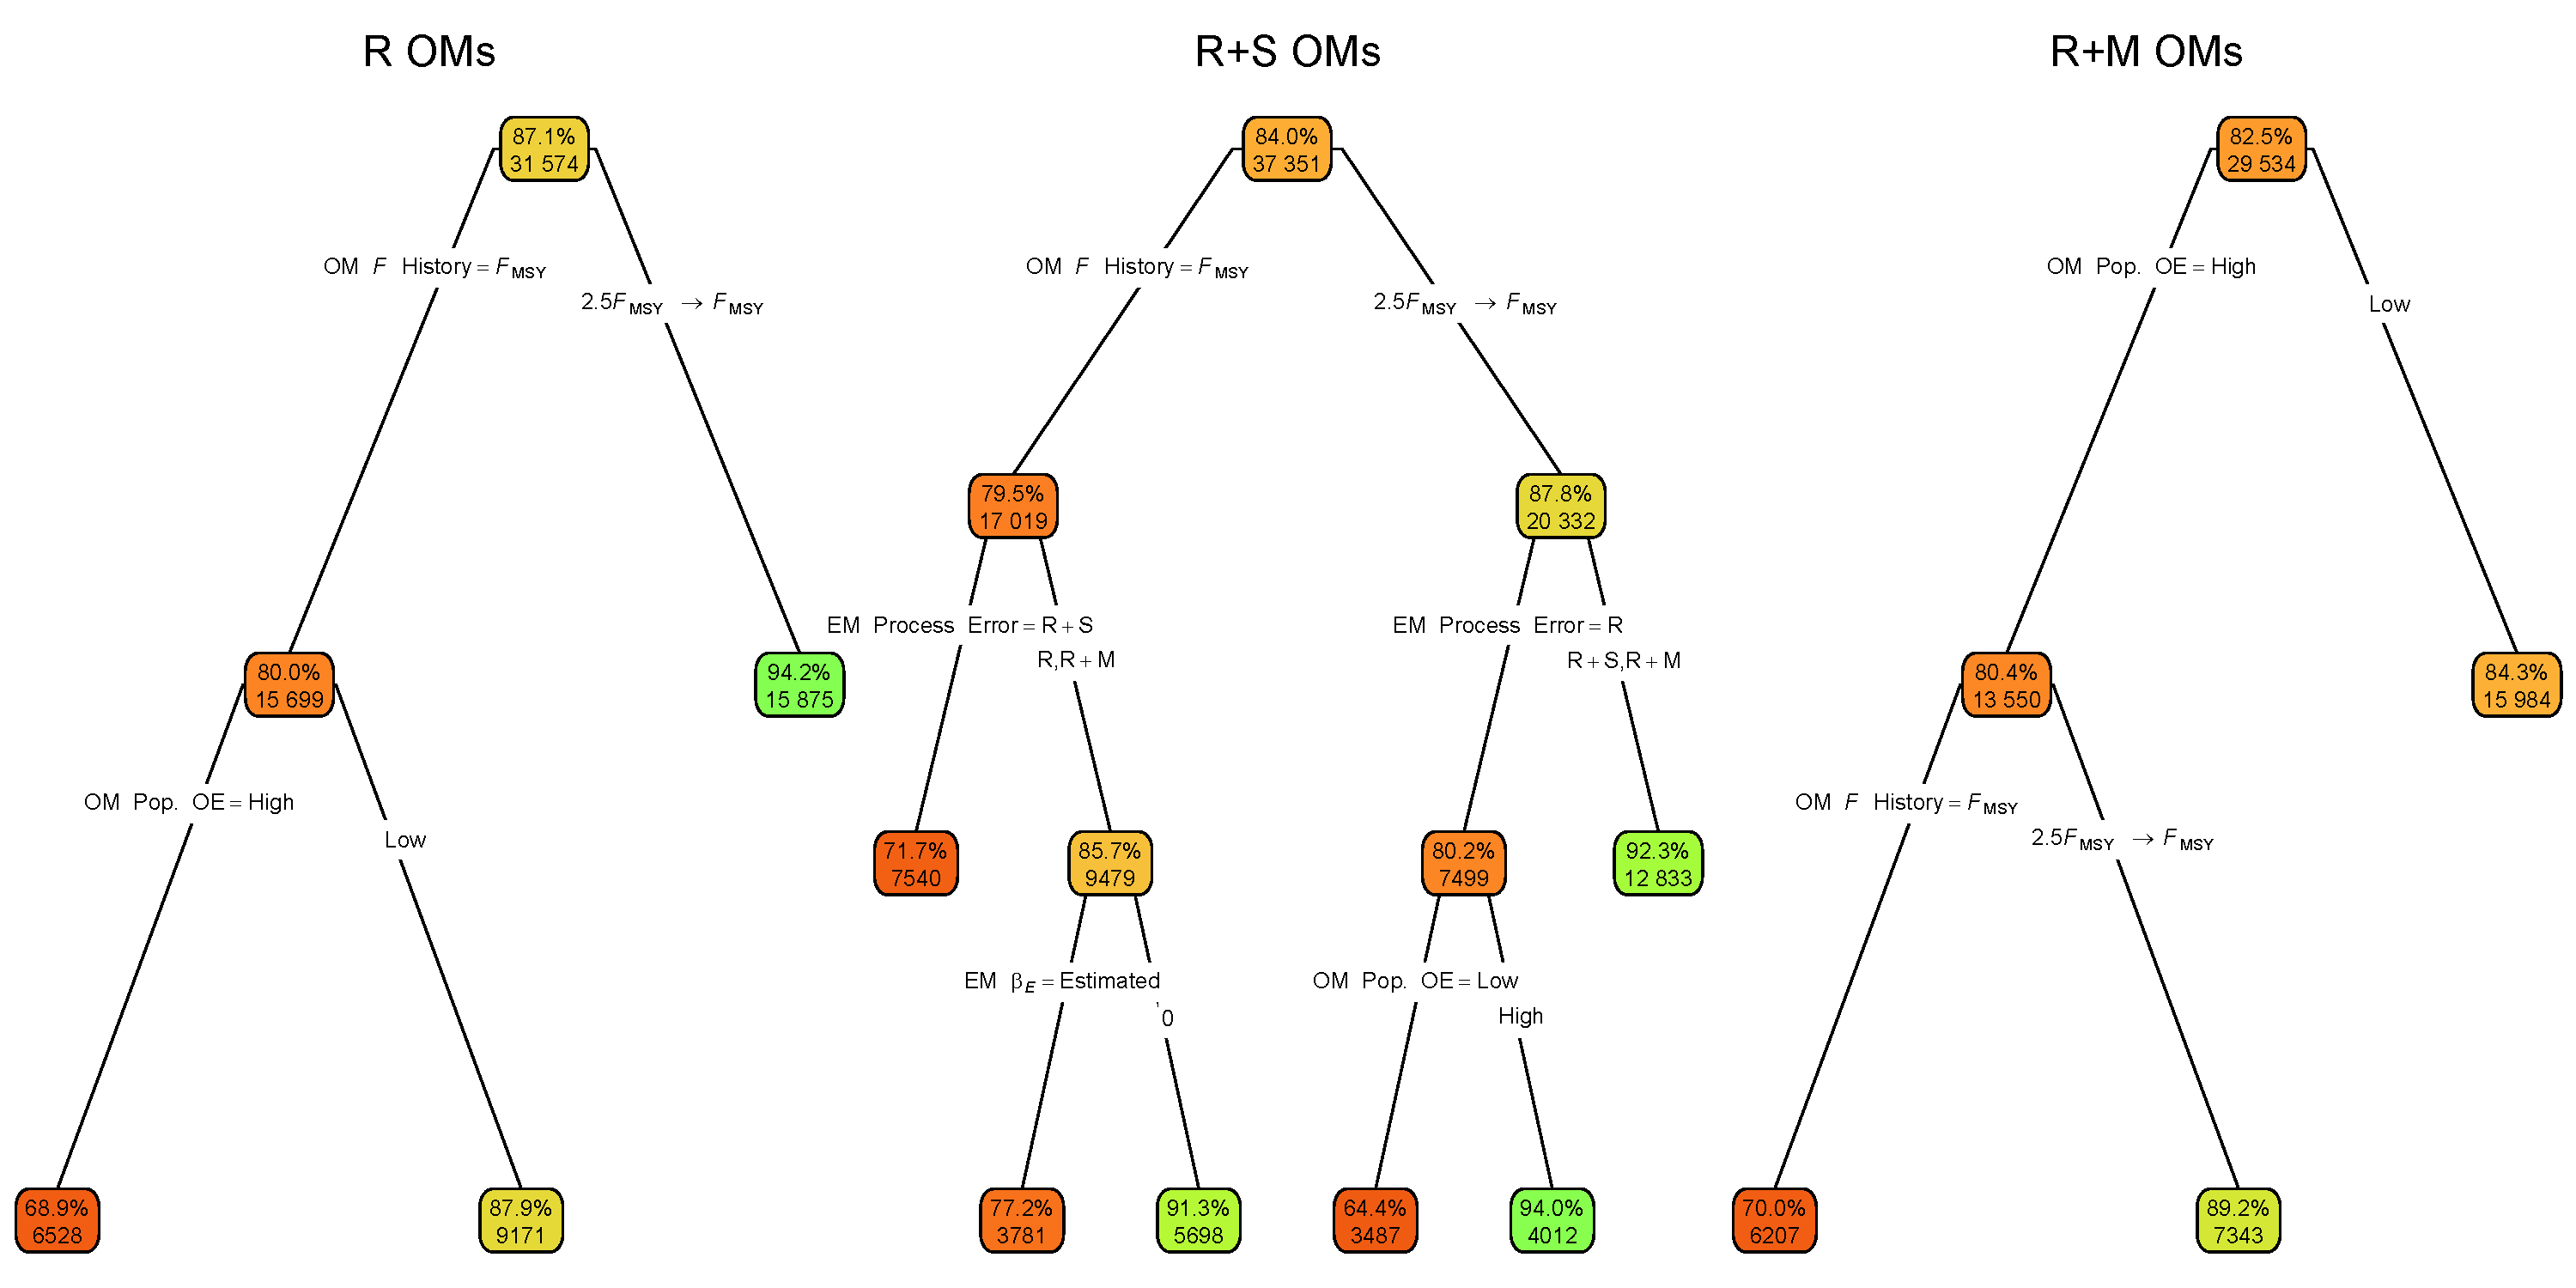
\includegraphics[width = 1.4\textwidth]{median_M_CI_coverage_regtree_plots}
\DIFaddendFL \end{center}
\caption{\DIFdelbeginFL \DIFdelFL{Median relative error }\DIFdelendFL \DIFaddbeginFL \DIFaddFL{Classification trees indicating primary factors determining whether confidence intervals for estimated median $M$ parameter }\DIFaddendFL (\DIFdelbeginFL \DIFdelFL{MRE}\DIFdelendFL \DIFaddbeginFL \DIFaddFL{$\beta_M$}\DIFaddendFL ) \DIFdelbeginFL \DIFdelFL{of estimates of natural mortality rate }\DIFdelendFL in \DIFdelbeginFL \DIFdelFL{the terminal year for }\DIFdelendFL \DIFaddbeginFL \DIFaddFL{estimating models (}\DIFaddendFL EMs\DIFaddbeginFL \DIFaddFL{) fitted to operating models (OMs) }\DIFaddendFL with \DIFdelbeginFL \DIFdelFL{alternative }\DIFdelendFL process error \DIFdelbeginFL \DIFdelFL{assumptions}\DIFdelendFL \DIFaddbeginFL \DIFaddFL{on recruitment only (R)}\DIFaddendFL , \DIFdelbeginFL \DIFdelFL{treatment of covariate effect }\DIFdelendFL \DIFaddbeginFL \DIFaddFL{recruitment and apparent survival }\DIFaddendFL (\DIFdelbeginFL \DIFdelFL{$\beta_E = 0$ or estimated}\DIFdelendFL \DIFaddbeginFL \DIFaddFL{R+S}\DIFaddendFL ), \DIFaddbeginFL \DIFaddFL{or recruitment }\DIFaddendFL and \DIFdelbeginFL \DIFdelFL{treatment of median }\DIFdelendFL natural mortality \DIFdelbeginFL \DIFdelFL{parameter }\DIFdelendFL (\DIFdelbeginFL \DIFdelFL{$\beta_M$ estimated or known}\DIFdelendFL \DIFaddbeginFL \DIFaddFL{R+M}\DIFaddendFL ) \DIFaddbeginFL \DIFaddFL{included the true value}\DIFaddendFL . \DIFdelbeginFL \DIFdelFL{All OMs had low observation }\DIFdelendFL \DIFaddbeginFL \DIFaddFL{Each node shows the median }\DIFaddendFL error \DIFaddbeginFL \DIFaddFL{(top) }\DIFaddendFL and \DIFdelbeginFL \DIFdelFL{contrast in fishing mortality}\DIFdelendFL \DIFaddbeginFL \DIFaddFL{number of observations (bottom) for the corresponding subset}\DIFaddendFL . \DIFaddbeginFL \DIFaddFL{Lower or higher median absolute errors of the process error assumption are indicated by more green or red polygons, respectively. See Table \ref{factor_table} for description of OM and EM factors defining nodes and branches.}\DIFaddendFL }\DIFdelbeginFL %DIFDELCMD < \label{terminal_M_bias}
%DIFDELCMD < %%%
\DIFdelendFL \DIFaddbeginFL \label{med_M_CI_coverage_regtree}
\DIFaddendFL \end{figure}
\end{landscape}

\begin{landscape}
\begin{figure}
\begin{center}
\DIFdelbeginFL %DIFDELCMD < 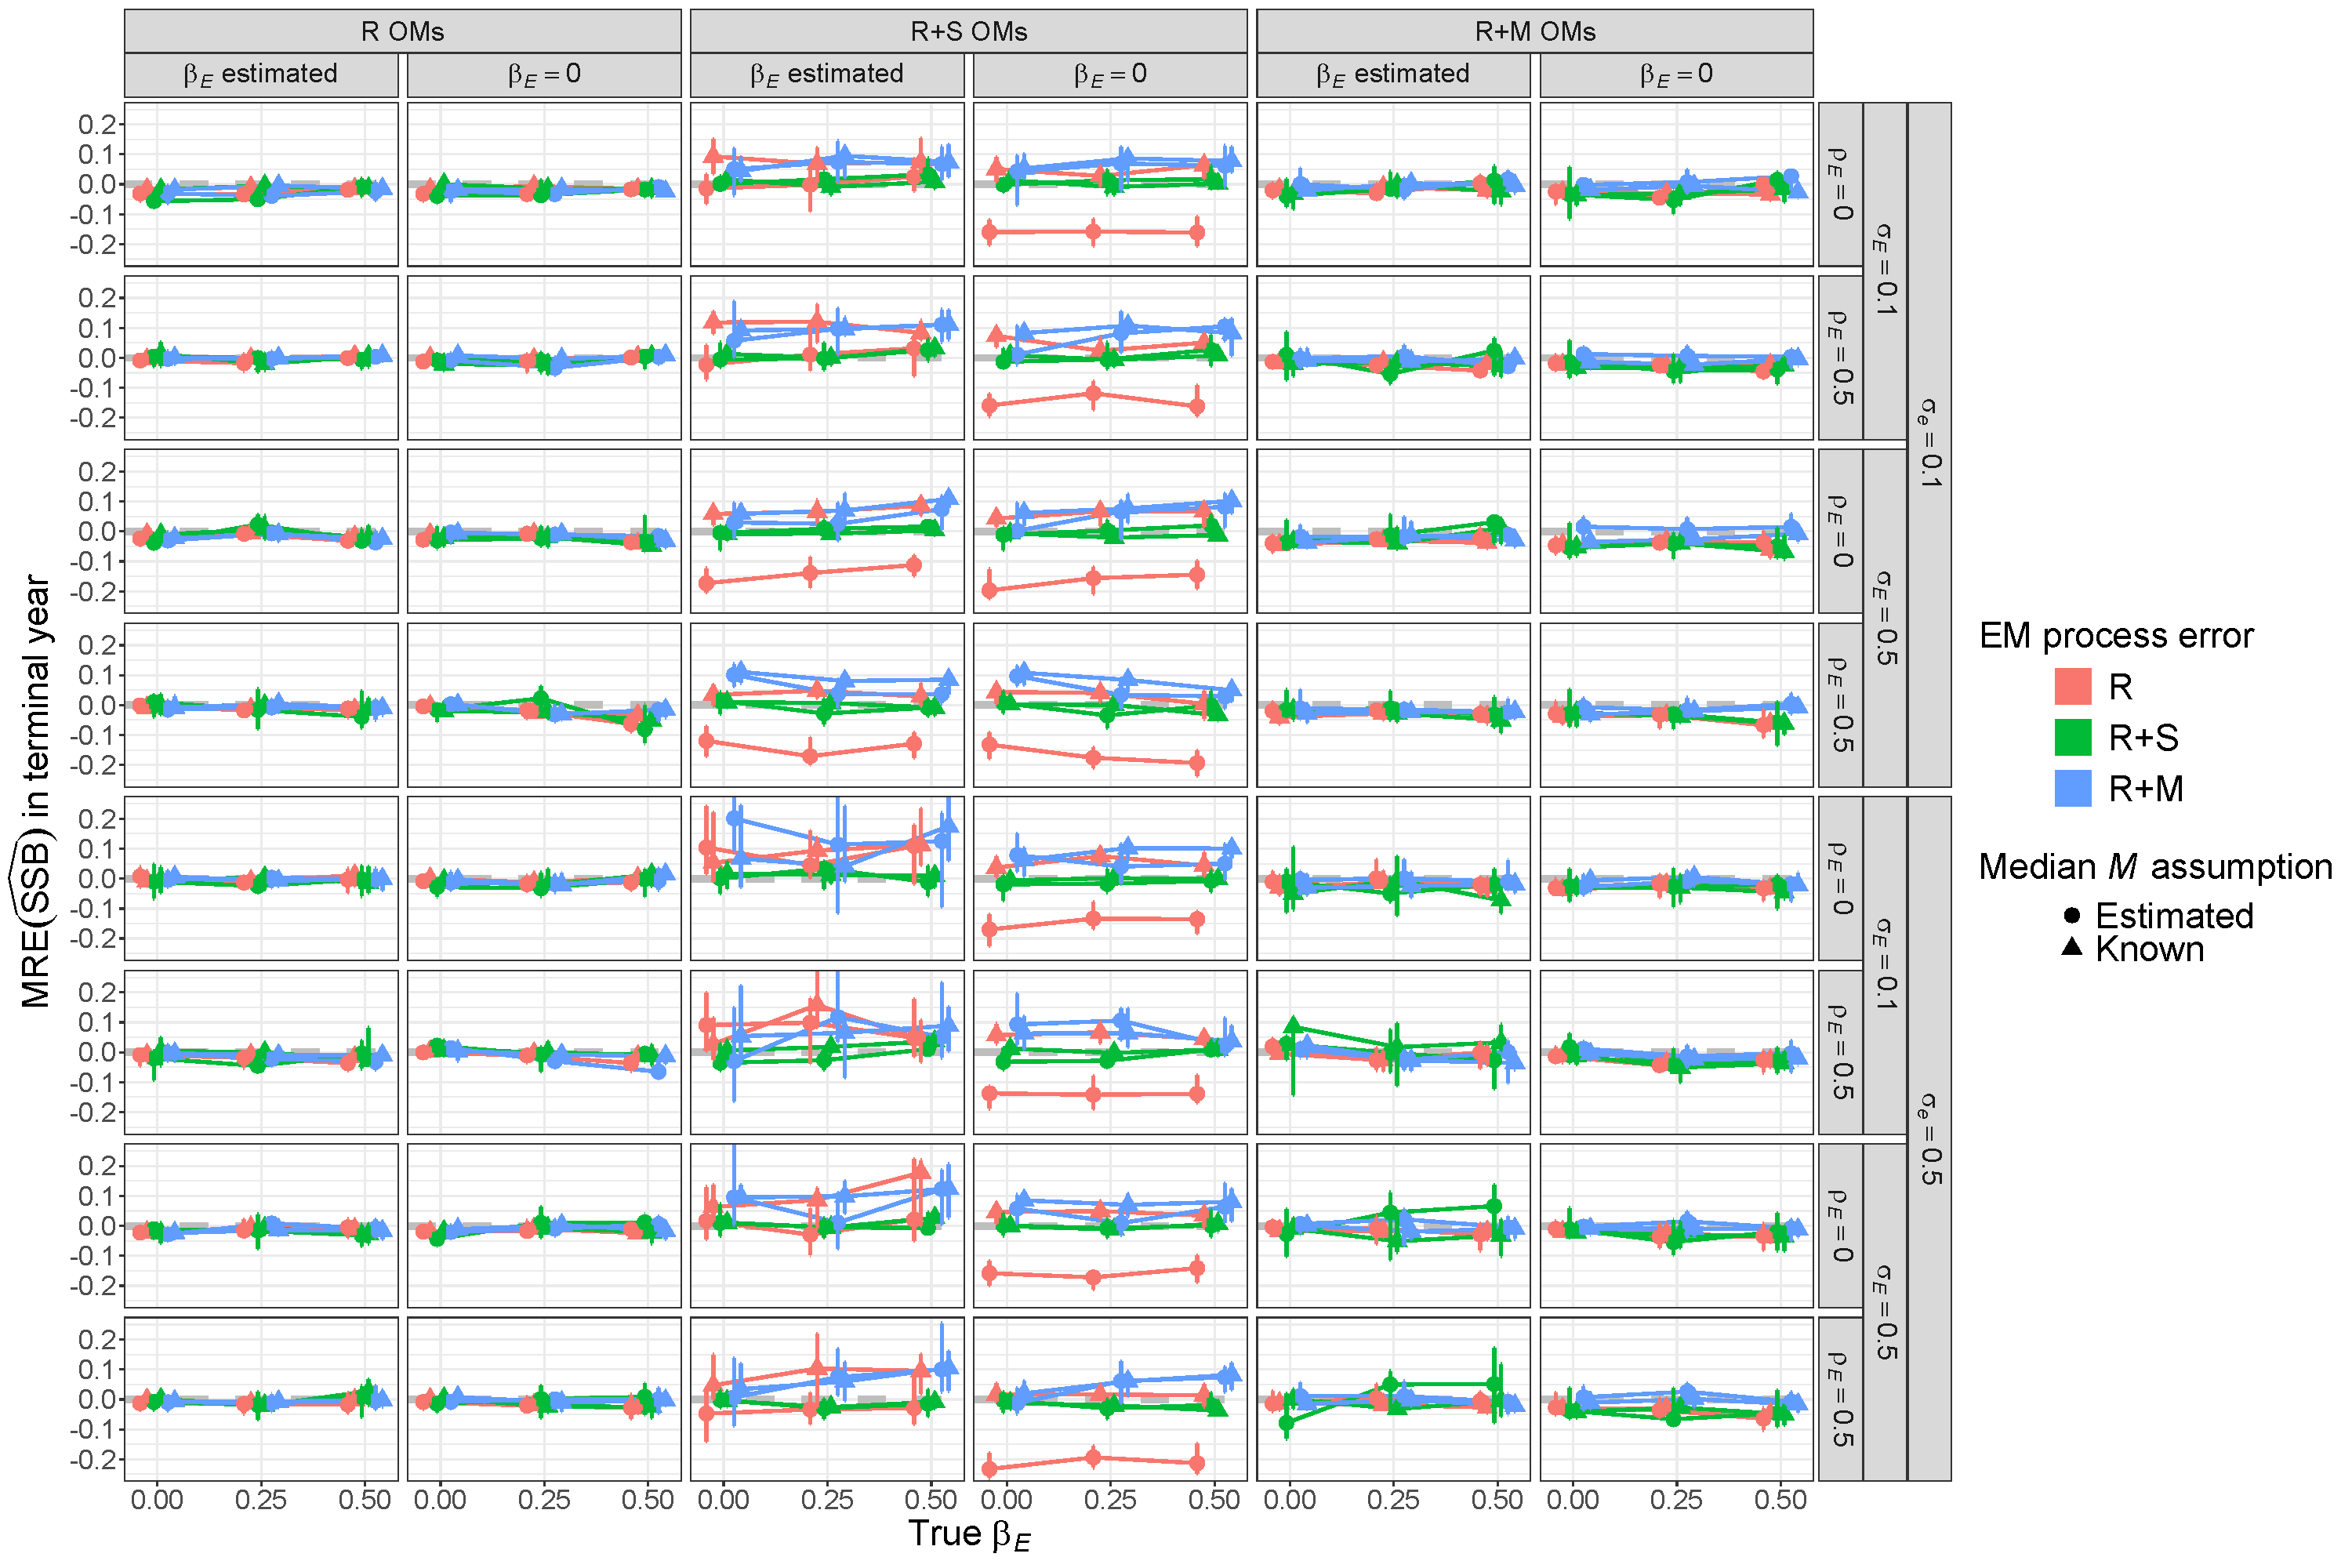
\includegraphics[height = \textheight]{terminal_year_ssb_bias_main}
%DIFDELCMD < %%%
\DIFdelendFL \DIFaddbeginFL 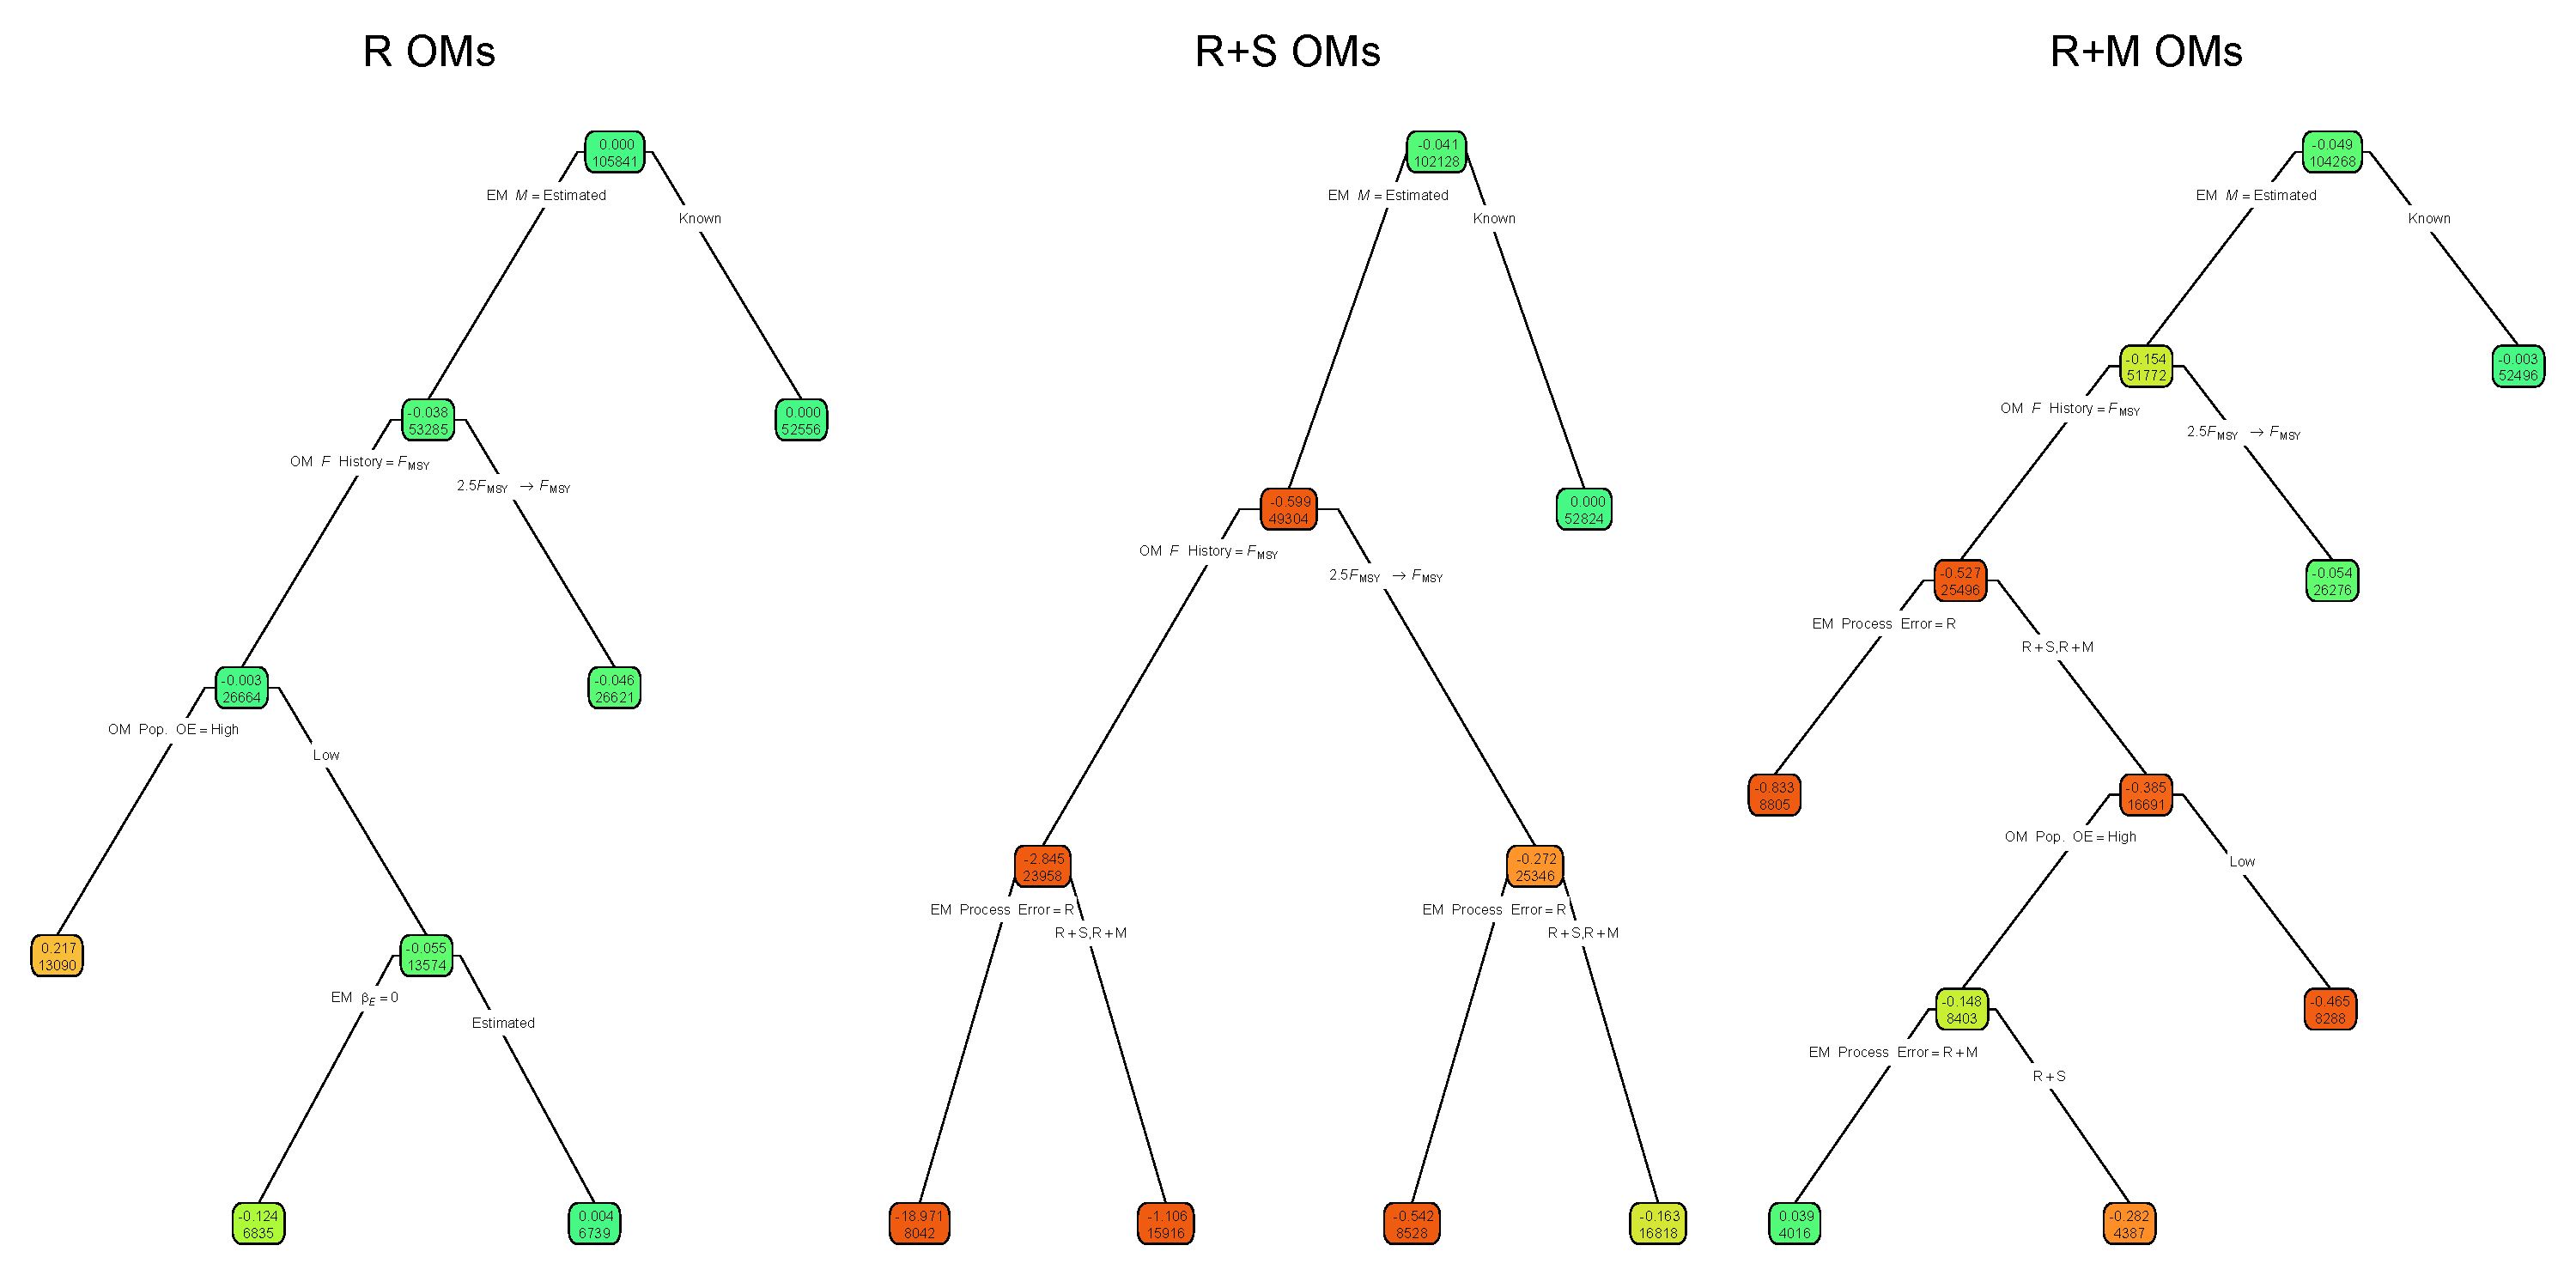
\includegraphics[width = 1.4\textwidth]{term_M_bias_regtree_plots}
\DIFaddendFL \end{center}
\caption{\DIFdelbeginFL \DIFdelFL{Median relative error (MRE) }\DIFdelendFL \DIFaddbeginFL \DIFaddFL{Regression trees indicating primary factors determining reductions in sums }\DIFaddendFL of \DIFdelbeginFL \DIFdelFL{estimates }\DIFdelendFL \DIFaddbeginFL \DIFaddFL{squares }\DIFaddendFL of \DIFdelbeginFL \DIFdelFL{spawning stock biomass (SSB) }\DIFdelendFL \DIFaddbeginFL \DIFaddFL{errors }\DIFaddendFL in \DIFaddbeginFL \DIFaddFL{estimation measured by Eq. \ref{relerror_trans_response} for }\DIFaddendFL the terminal year \DIFdelbeginFL \DIFdelFL{for }\DIFdelendFL \DIFaddbeginFL \DIFaddFL{$M$ in estimating models (}\DIFaddendFL EMs\DIFaddbeginFL \DIFaddFL{) fitted to operating models (OMs) }\DIFaddendFL with \DIFdelbeginFL \DIFdelFL{alternative }\DIFdelendFL process error \DIFdelbeginFL \DIFdelFL{assumptions}\DIFdelendFL \DIFaddbeginFL \DIFaddFL{on recruitment only (R)}\DIFaddendFL , \DIFdelbeginFL \DIFdelFL{treatment of covariate effect }\DIFdelendFL \DIFaddbeginFL \DIFaddFL{recruitment and apparent survival }\DIFaddendFL (\DIFdelbeginFL \DIFdelFL{$\beta_E = 0$ or estimated}\DIFdelendFL \DIFaddbeginFL \DIFaddFL{R+S}\DIFaddendFL ), \DIFaddbeginFL \DIFaddFL{or recruitment }\DIFaddendFL and \DIFdelbeginFL \DIFdelFL{treatment of median }\DIFdelendFL natural mortality \DIFdelbeginFL \DIFdelFL{parameter }\DIFdelendFL (\DIFdelbeginFL \DIFdelFL{$\beta_M$ estimated or known}\DIFdelendFL \DIFaddbeginFL \DIFaddFL{R+M}\DIFaddendFL ). \DIFdelbeginFL \DIFdelFL{All OMs had low observation }\DIFdelendFL \DIFaddbeginFL \DIFaddFL{Each node shows the median }\DIFaddendFL error \DIFaddbeginFL \DIFaddFL{(top) }\DIFaddendFL and \DIFdelbeginFL \DIFdelFL{contrast in fishing mortality}\DIFdelendFL \DIFaddbeginFL \DIFaddFL{number of observations (bottom) for the corresponding subset}\DIFaddendFL . \DIFaddbeginFL \DIFaddFL{Lower or higher median absolute errors of the process error assumption are indicated by more green or red polygons, respectively. See Table \ref{factor_table} for description of OM and EM factors defining nodes and branches.}\DIFaddendFL }\DIFdelbeginFL %DIFDELCMD < \label{terminal_ssb_bias}
%DIFDELCMD < %%%
\DIFdelendFL \DIFaddbeginFL \label{term_M_bias_regtree}
\DIFaddendFL \end{figure}
\end{landscape}

\DIFdelbegin %DIFDELCMD < \hypertarget{supplemental-materials}{%
%DIFDELCMD < \section*{Supplemental Materials}\label{supplemental-materials}}
%DIFDELCMD < %%%
\addcontentsline{toc}{section}{\DIFdel{Supplemental Materials}}
%DIFAUXCMD
\DIFdelend \DIFaddbegin \begin{landscape}
\begin{figure}
\begin{center}
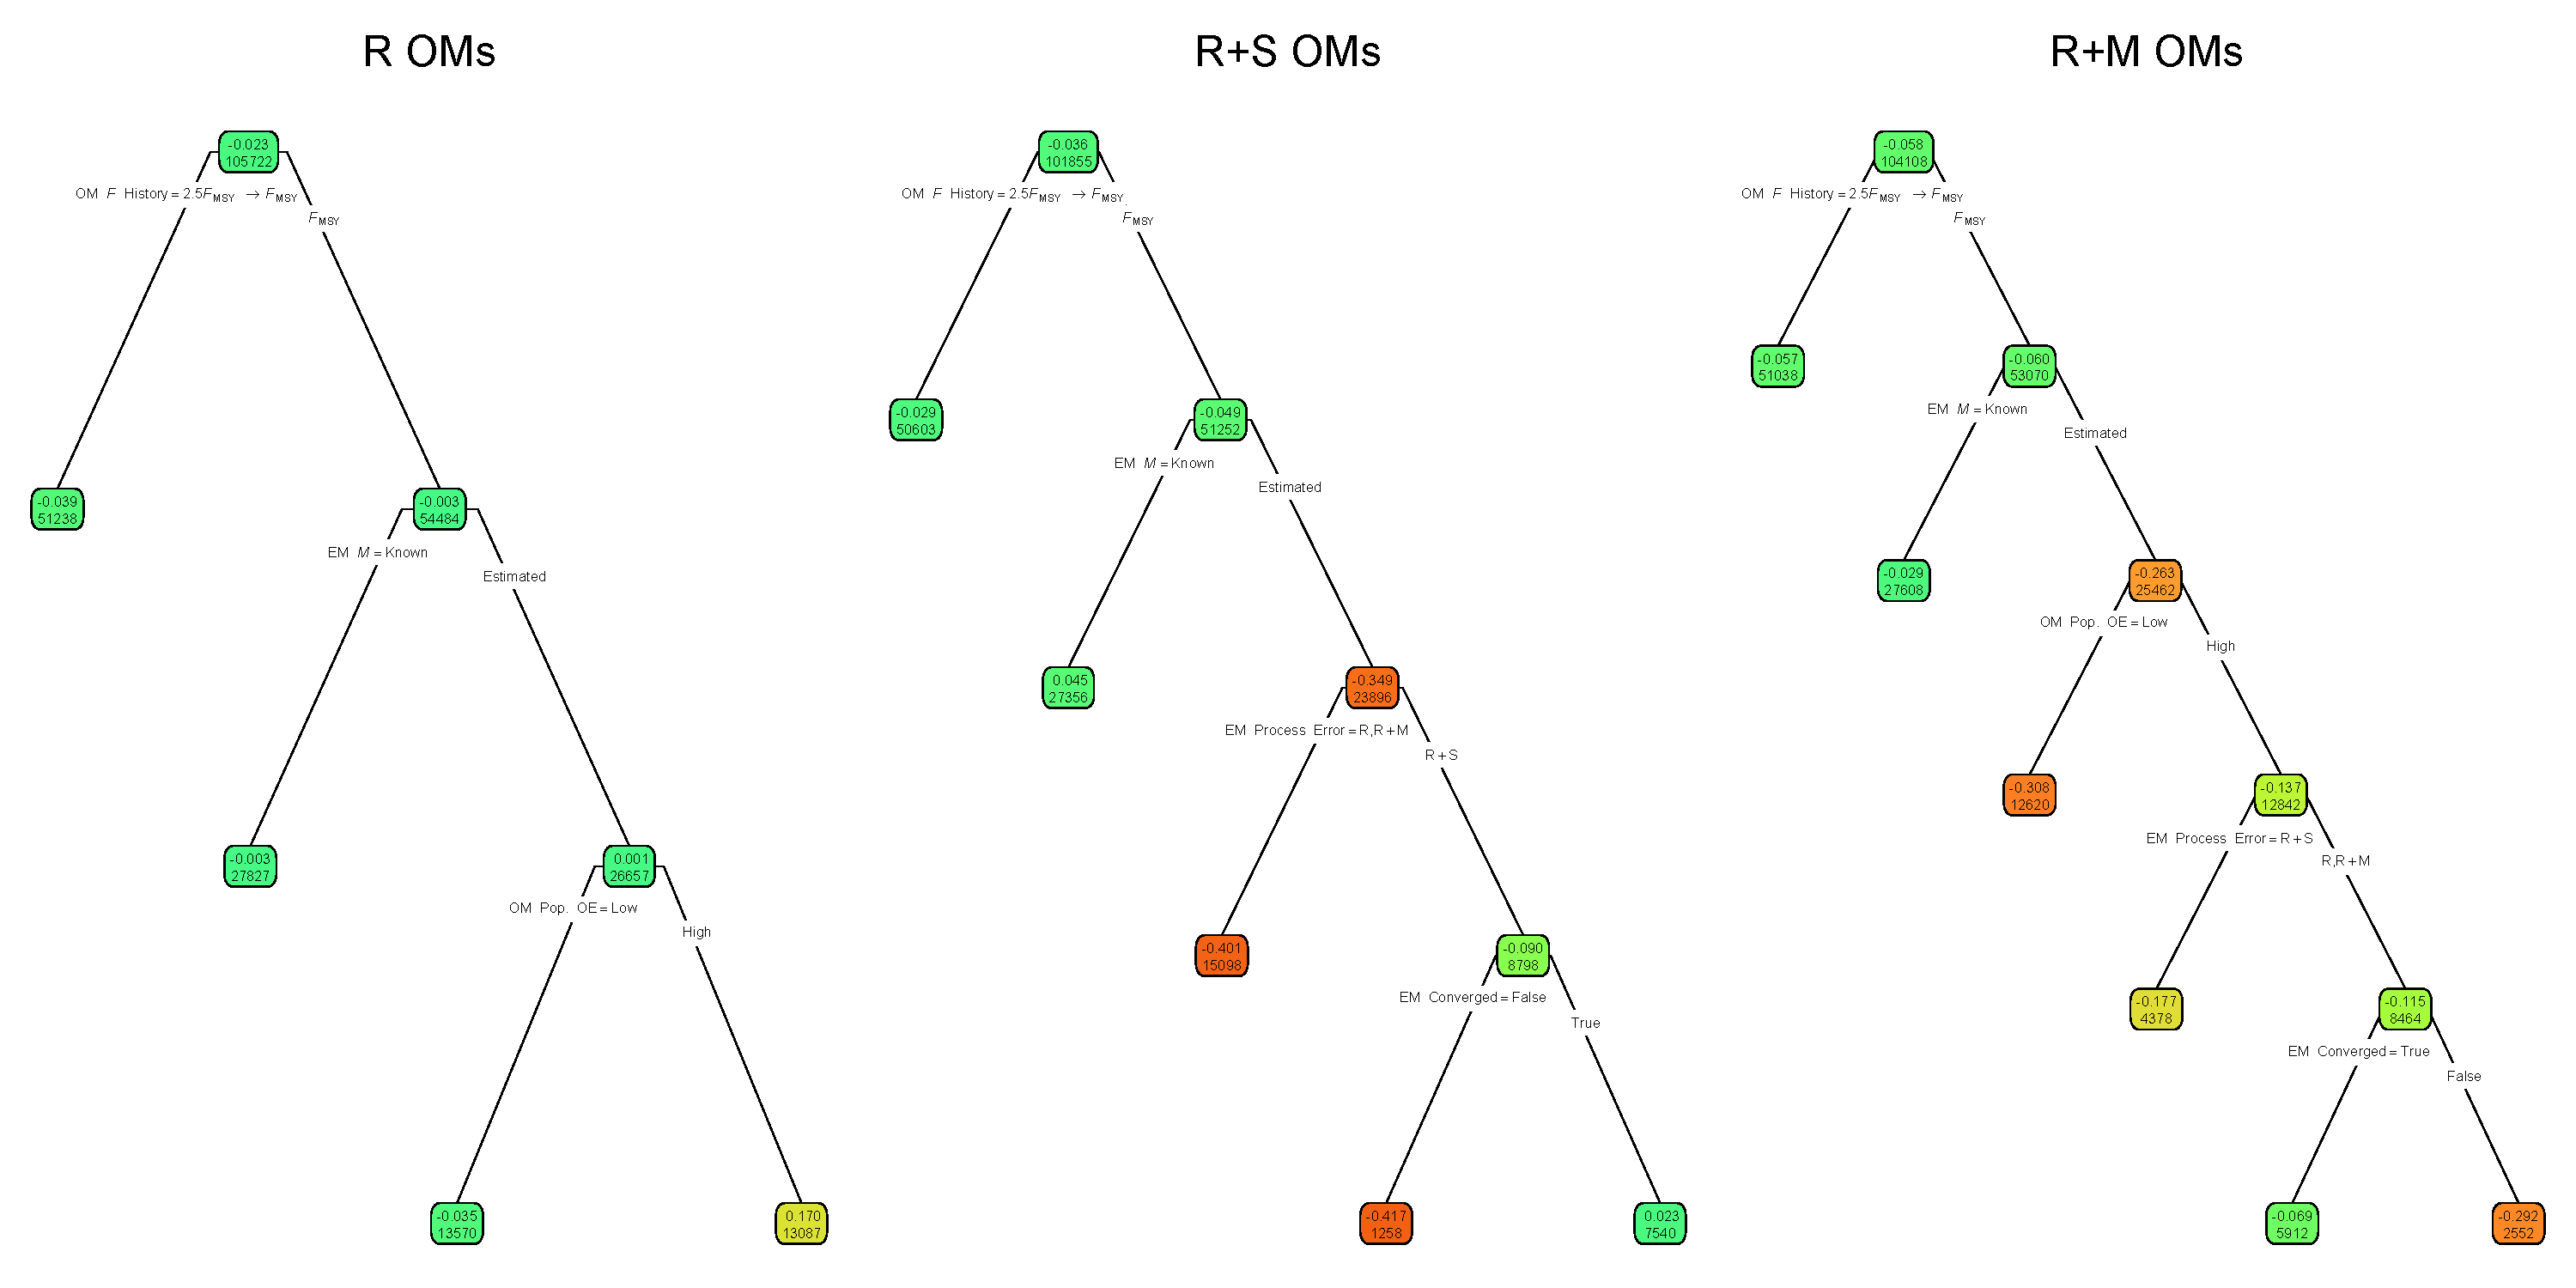
\includegraphics[width = 1.4\textwidth]{term_SSB_bias_regtree_plots}
\end{center}
\caption{\DIFaddFL{Regression trees indicating primary factors determining reductions in sums of squares of errors in estimation measured by Eq. \ref{relerror_trans_response} for the terminal year SSB in estimating models (EMs) fitted to operating models (OMs) with process error on recruitment only (R), recruitment and apparent survival (R+S), or recruitment and natural mortality (R+M). Each node shows the median error (top) and number of observations (bottom) for the corresponding subset. Lower or higher median absolute errors of the process error assumption are indicated by more green or red polygons, respectively. See Table \ref{factor_table} for description of OM and EM factors defining nodes and branches.}}\label{term_SSB_bias_regtree}
\end{figure}
\end{landscape}
\DIFaddend 

\DIFaddbegin \pagebreak

\begin{table}
\caption{\DIFaddFL{For operating models (OMs) with process error on recruitment only (R), recruitment and apparent survival (R+S), or recruitment and natural mortality (R+M) (columns), the percent reduction in deviance for logistic regression models fit to indicators of convergence (providing Hessian-based standard errors) with each OM and estimating model (EM) factor (rows) included individually, combined, and with second and third order interactions.}}\label{convergence_PRD_table}
{\begin{center}
\begin{tabular}{lrrr}
\hline\hline
\multicolumn{1}{l}{\DIFaddFL{Factor}}&\multicolumn{1}{c}{\DIFaddFL{R}}&\multicolumn{1}{c}{\DIFaddFL{R+S}}&\multicolumn{1}{c}{\DIFaddFL{R+M}}\tabularnewline
\hline
\DIFaddFL{OM $F$ history}& \DIFaddFL{0.86}&\DIFaddFL{\textless  0.01}& \DIFaddFL{0.24}\tabularnewline
\DIFaddFL{OM Obs. Error}& \DIFaddFL{0.56}& \DIFaddFL{0.03}& \DIFaddFL{0.26}\tabularnewline
\DIFaddFL{OM $\sigma_e$}& \DIFaddFL{0.66}& \DIFaddFL{2.99}& \DIFaddFL{0.93}\tabularnewline
\DIFaddFL{OM $\sigma_E$}& \DIFaddFL{0.53}& \DIFaddFL{2.22}& \DIFaddFL{0.62}\tabularnewline
\DIFaddFL{OM $\rho_{E}$}&\DIFaddFL{\textless  0.01}& \DIFaddFL{0.02}&\DIFaddFL{\textless  0.01}\tabularnewline
\DIFaddFL{OM $\beta_{E}$}& \DIFaddFL{0.02}&\DIFaddFL{\textless  0.01}&\DIFaddFL{\textless  0.01}\tabularnewline
\DIFaddFL{EM Process Error}&\DIFaddFL{24.53}& \DIFaddFL{9.33}&\DIFaddFL{23.06}\tabularnewline
\DIFaddFL{EM $\beta_{E}$ assumption}& \DIFaddFL{0.16}& \DIFaddFL{2.96}& \DIFaddFL{0.51}\tabularnewline
\DIFaddFL{EM $M$ Assumption}& \DIFaddFL{0.18}& \DIFaddFL{2.83}& \DIFaddFL{0.40}\tabularnewline
\DIFaddFL{All factors}&\DIFaddFL{28.92}&\DIFaddFL{22.67}&\DIFaddFL{27.34}\tabularnewline
\DIFaddFL{+ All Two Way}&\DIFaddFL{36.15}&\DIFaddFL{33.54}&\DIFaddFL{34.03}\tabularnewline
\DIFaddFL{+ All Three Way}&\DIFaddFL{37.95}&\DIFaddFL{36.58}&\DIFaddFL{35.57}\tabularnewline
\hline
\end{tabular}\end{center}
}
\end{table}
\pagebreak

\begin{table}
\caption{\DIFaddFL{For eoperating models (OMs) with process error on recruitment only (R), recruitment and apparent survival (R+S), or recruitment and natural mortality (R+M) (columns), the percent reduction in deviance for multinomial logistic regression models fit to indicators of process error assumption in the estimating models (EMs) with lowest AIC with each OM and EM factor (rows) included individually, combined, and with second and third order interactions.}}\label{AIC_PE_PRD_table}
{\begin{center}
\begin{tabular}{lrrr}
\hline\hline
\multicolumn{1}{l}{\DIFaddFL{Factor}}&\multicolumn{1}{c}{\DIFaddFL{R}}&\multicolumn{1}{c}{\DIFaddFL{R+S}}&\multicolumn{1}{c}{\DIFaddFL{R+M}}\tabularnewline
\hline
\DIFaddFL{OM $F$ history}& \DIFaddFL{0.23}& \DIFaddFL{0.06}& \DIFaddFL{0.30}\tabularnewline
\DIFaddFL{OM Obs. Error}& \DIFaddFL{0.54}&\DIFaddFL{18.58}&\DIFaddFL{13.43}\tabularnewline
\DIFaddFL{OM $\sigma_e$}& \DIFaddFL{8.41}& \DIFaddFL{0.05}& \DIFaddFL{2.23}\tabularnewline
\DIFaddFL{OM $\sigma_E$}& \DIFaddFL{0.17}& \DIFaddFL{0.08}& \DIFaddFL{0.59}\tabularnewline
\DIFaddFL{OM $\rho_{E}$}& \DIFaddFL{1.29}& \DIFaddFL{0.03}& \DIFaddFL{0.06}\tabularnewline
\DIFaddFL{OM $\beta_{E}$}& \DIFaddFL{3.42}& \DIFaddFL{0.04}& \DIFaddFL{0.38}\tabularnewline
\DIFaddFL{EM $M$ Assumption}& \DIFaddFL{0.35}& \DIFaddFL{0.34}& \DIFaddFL{0.48}\tabularnewline
\DIFaddFL{EM $\beta_{E}$ Assumption Correct}& \DIFaddFL{2.35}& \DIFaddFL{0.22}& \DIFaddFL{0.78}\tabularnewline
\DIFaddFL{All factors}&\DIFaddFL{21.97}&\DIFaddFL{19.29}&\DIFaddFL{19.07}\tabularnewline
\DIFaddFL{+ All Two Way}&\DIFaddFL{38.25}&\DIFaddFL{21.13}&\DIFaddFL{24.73}\tabularnewline
\DIFaddFL{+ All Three Way}&\DIFaddFL{46.26}&\DIFaddFL{22.85}&\DIFaddFL{26.97}\tabularnewline
\hline
\end{tabular}\end{center}
}
\end{table}
\pagebreak

\begin{table}
\caption{\DIFaddFL{For each operating model (OM) covariate effect assumption (columns), the percent reduction in deviance for logistic regression models fit to indicators of correct estimating model (EM) covariate effect assumption (no effect with OM $\beta_E = 0$ or estimated effect when OM $\beta_E > 0$) with lowest AIC with each OM and EM factor (rows) included individually, combined, and with second and third order interactions.}}\label{AIC_Ecov_effect_PRD_table}
{\begin{center}
\begin{tabular}{lrrr}
\hline\hline
\multicolumn{1}{l}{\DIFaddFL{Factor}}&\multicolumn{1}{c}{\DIFaddFL{$\beta_E = 0$}}&\multicolumn{1}{c}{\DIFaddFL{$\beta_E = 0.25$}}&\multicolumn{1}{c}{\DIFaddFL{$\beta_E = 0.5$}}\tabularnewline
\hline
\DIFaddFL{OM $F$ history}&\DIFaddFL{\textless  0.01}& \DIFaddFL{0.09}& \DIFaddFL{0.18}\tabularnewline
\DIFaddFL{OM Obs. Error}& \DIFaddFL{1.19}& \DIFaddFL{4.06}& \DIFaddFL{4.64}\tabularnewline
\DIFaddFL{OM Process Error}& \DIFaddFL{4.11}& \DIFaddFL{0.71}& \DIFaddFL{0.25}\tabularnewline
\DIFaddFL{OM $\sigma_e$}& \DIFaddFL{0.66}& \DIFaddFL{2.00}& \DIFaddFL{1.97}\tabularnewline
\DIFaddFL{OM $\sigma_E$}& \DIFaddFL{0.35}& \DIFaddFL{7.97}&\DIFaddFL{20.66}\tabularnewline
\DIFaddFL{OM $\rho_{E}$}& \DIFaddFL{0.21}& \DIFaddFL{1.23}& \DIFaddFL{1.48}\tabularnewline
\DIFaddFL{EM $M$ Assumption}& \DIFaddFL{0.23}& \DIFaddFL{0.15}& \DIFaddFL{0.15}\tabularnewline
\DIFaddFL{EM Process Error Assumption Correct}& \DIFaddFL{1.95}& \DIFaddFL{0.39}& \DIFaddFL{0.06}\tabularnewline
\DIFaddFL{All factors}& \DIFaddFL{6.95}&\DIFaddFL{17.65}&\DIFaddFL{33.44}\tabularnewline
\DIFaddFL{+ All Two Way}&\DIFaddFL{10.58}&\DIFaddFL{23.21}&\DIFaddFL{38.36}\tabularnewline
\DIFaddFL{+ All Three Way}&\DIFaddFL{11.83}&\DIFaddFL{24.95}&\DIFaddFL{39.79}\tabularnewline
\hline
\end{tabular}\end{center}
}
\end{table}
\pagebreak

\begin{table}
\caption{\DIFaddFL{For operating models (OMs) with process error on recruitment only (R), recruitment and apparent survival (R+S), or recruitment and natural mortality (R+M)  (columns), the percent reduction in deviance for linear regression models fit to errors in estimation of the covariate effect on natural mortality rate ($\widehat \beta_E$) with each OM and estimating model (EM) factor (rows) included individually, combined, and with second and third order interactions.}}\label{bias_ecov_beta_converged_PRD_table}
{\begin{center}
\begin{tabular}{lrrr}
\hline\hline
\multicolumn{1}{l}{\DIFaddFL{Factor}}&\multicolumn{1}{c}{\DIFaddFL{R}}&\multicolumn{1}{c}{\DIFaddFL{R+S}}&\multicolumn{1}{c}{\DIFaddFL{R+M}}\tabularnewline
\hline
\DIFaddFL{OM $F$ history}&\DIFaddFL{0.03}&\DIFaddFL{0.06}&\DIFaddFL{0.02}\tabularnewline
\DIFaddFL{OM Obs. Error}&\DIFaddFL{\textless  0.01}&\DIFaddFL{0.06}&\DIFaddFL{0.02}\tabularnewline
\DIFaddFL{OM $\sigma_e$}&\DIFaddFL{0.04}&\DIFaddFL{0.08}&\DIFaddFL{0.06}\tabularnewline
\DIFaddFL{OM $\sigma_E$}&\DIFaddFL{\textless  0.01}&\DIFaddFL{0.02}&\DIFaddFL{0.01}\tabularnewline
\DIFaddFL{OM $\rho_{E}$}&\DIFaddFL{\textless  0.01}&\DIFaddFL{0.01}&\DIFaddFL{\textless  0.01}\tabularnewline
\DIFaddFL{OM $\beta_{E}$}&\DIFaddFL{0.05}&\DIFaddFL{\textless  0.01}&\DIFaddFL{\textless  0.01}\tabularnewline
\DIFaddFL{EM Process Error}&\DIFaddFL{0.01}&\DIFaddFL{0.06}&\DIFaddFL{0.01}\tabularnewline
\DIFaddFL{EM $M$ assumption}&\DIFaddFL{0.02}&\DIFaddFL{0.02}&\DIFaddFL{\textless  0.01}\tabularnewline
\DIFaddFL{All factors}&\DIFaddFL{0.18}&\DIFaddFL{0.37}&\DIFaddFL{0.14}\tabularnewline
\DIFaddFL{+ All Two Way}&\DIFaddFL{0.50}&\DIFaddFL{1.11}&\DIFaddFL{0.35}\tabularnewline
\DIFaddFL{+ All Three Way}&\DIFaddFL{1.38}&\DIFaddFL{1.88}&\DIFaddFL{0.66}\tabularnewline
\hline
\end{tabular}\end{center}
}
\end{table}
\pagebreak

\begin{table}
\caption{\DIFaddFL{For operating models (OMs) with process error on recruitment only (R), recruitment and apparent survival (R+S), or recruitment and natural mortality (R+M) (columns), the percent reduction in deviance for logistic regression models fit to indicators of whether confidence intervals for covariate effect estimates includes the true value with each OM and estimating model (EM) factor (rows) included individually, combined, and with second and third order interactions.}}\label{ecov_beta_ci_coverage_PRD_table}
{\begin{center}
\begin{tabular}{lrrr}
\hline\hline
\multicolumn{1}{l}{\DIFaddFL{Factor}}&\multicolumn{1}{c}{\DIFaddFL{R}}&\multicolumn{1}{c}{\DIFaddFL{R+S}}&\multicolumn{1}{c}{\DIFaddFL{R+M}}\tabularnewline
\hline
\DIFaddFL{OM $F$ history}& \DIFaddFL{0.24}& \DIFaddFL{0.05}& \DIFaddFL{0.01}\tabularnewline
\DIFaddFL{OM Obs. Error}& \DIFaddFL{1.36}& \DIFaddFL{1.91}& \DIFaddFL{1.78}\tabularnewline
\DIFaddFL{OM $\sigma_e$}& \DIFaddFL{8.26}& \DIFaddFL{0.24}& \DIFaddFL{0.92}\tabularnewline
\DIFaddFL{OM $\sigma_E$}& \DIFaddFL{0.92}& \DIFaddFL{1.70}& \DIFaddFL{1.56}\tabularnewline
\DIFaddFL{OM $\rho_{E}$}& \DIFaddFL{0.03}& \DIFaddFL{0.05}& \DIFaddFL{0.06}\tabularnewline
\DIFaddFL{OM $\beta_{E}$}&\DIFaddFL{11.10}& \DIFaddFL{0.68}& \DIFaddFL{2.72}\tabularnewline
\DIFaddFL{EM Process Error}& \DIFaddFL{0.01}& \DIFaddFL{6.51}& \DIFaddFL{0.27}\tabularnewline
\DIFaddFL{EM $M$ assumption}& \DIFaddFL{0.25}& \DIFaddFL{0.29}& \DIFaddFL{0.06}\tabularnewline
\DIFaddFL{All factors}&\DIFaddFL{23.61}&\DIFaddFL{12.16}& \DIFaddFL{7.78}\tabularnewline
\DIFaddFL{+ All Two Way}&\DIFaddFL{30.17}&\DIFaddFL{18.08}&\DIFaddFL{12.63}\tabularnewline
\DIFaddFL{+ All Three Way}&\DIFaddFL{32.58}&\DIFaddFL{20.62}&\DIFaddFL{14.87}\tabularnewline
\hline
\end{tabular}\end{center}
}
\end{table}
\pagebreak

\begin{table}
\caption{\DIFaddFL{For operating models (OMs) with process error on recruitment only (R), recruitment and apparent survival (R+S), or recruitment and natural mortality (R+M) (columns), the percent reduction in deviance for linear regression models fit to errors in estimation of the median natural mortality rate parameter ($\widehat \beta_M$) with each OM and estimating model (EM) factor (rows) included individually, combined, and with second and third order interactions.}}\label{bias_median_M_converged_PRD_table}
{\begin{center}
\begin{tabular}{lrrr}
\hline\hline
\multicolumn{1}{l}{\DIFaddFL{Factor}}&\multicolumn{1}{c}{\DIFaddFL{R}}&\multicolumn{1}{c}{\DIFaddFL{R+S}}&\multicolumn{1}{c}{\DIFaddFL{R+M}}\tabularnewline
\hline
\DIFaddFL{OM $F$ history}& \DIFaddFL{4.03}&\DIFaddFL{16.52}& \DIFaddFL{6.51}\tabularnewline
\DIFaddFL{OM Obs. Error}& \DIFaddFL{2.74}& \DIFaddFL{0.54}& \DIFaddFL{0.64}\tabularnewline
\DIFaddFL{OM $\sigma_e$}& \DIFaddFL{0.01}&\DIFaddFL{\textless  0.01}& \DIFaddFL{0.01}\tabularnewline
\DIFaddFL{OM $\sigma_E$}& \DIFaddFL{0.18}& \DIFaddFL{0.02}& \DIFaddFL{0.15}\tabularnewline
\DIFaddFL{OM $\rho_{E}$}& \DIFaddFL{0.07}& \DIFaddFL{0.05}&\DIFaddFL{\textless  0.01}\tabularnewline
\DIFaddFL{OM $\beta_{E}$}& \DIFaddFL{0.37}& \DIFaddFL{0.04}& \DIFaddFL{0.10}\tabularnewline
\DIFaddFL{EM Process Error}& \DIFaddFL{2.31}&\DIFaddFL{11.99}& \DIFaddFL{2.65}\tabularnewline
\DIFaddFL{EM $\beta_{E}$ assumption}& \DIFaddFL{2.83}& \DIFaddFL{7.20}& \DIFaddFL{3.25}\tabularnewline
\DIFaddFL{All factors}&\DIFaddFL{12.14}&\DIFaddFL{33.71}&\DIFaddFL{12.81}\tabularnewline
\DIFaddFL{+ All Two Way}&\DIFaddFL{21.74}&\DIFaddFL{46.46}&\DIFaddFL{19.84}\tabularnewline
\DIFaddFL{+ All Three Way}&\DIFaddFL{26.38}&\DIFaddFL{49.41}&\DIFaddFL{22.24}\tabularnewline
\hline
\end{tabular}\end{center}
}
\end{table}
\pagebreak

\begin{table}
\caption{\DIFaddFL{For operating models (OMs) with process error on recruitment only (R), recruitment and apparent survival (R+S), or recruitment and natural mortality (R+M) (columns), the percent reduction in deviance for logistic regression models fit to indicators of whether confidence intervals for estimates of the median natural mortality rate parameter ($\widehat \beta_M$) includes the true value with each OM and estimating model (EM) factor (rows) included individually, combined, and with second and third order interactions.}}\label{mean_M_ci_coverage_PRD_table}
{\begin{center}
\begin{tabular}{lrrr}
\hline\hline
\multicolumn{1}{l}{\DIFaddFL{Factor}}&\multicolumn{1}{c}{\DIFaddFL{R}}&\multicolumn{1}{c}{\DIFaddFL{R+S}}&\multicolumn{1}{c}{\DIFaddFL{R+M}}\tabularnewline
\hline
\DIFaddFL{OM $F$ history}& \DIFaddFL{6.08}& \DIFaddFL{1.46}& \DIFaddFL{0.14}\tabularnewline
\DIFaddFL{OM Obs. Error}& \DIFaddFL{1.48}& \DIFaddFL{0.41}& \DIFaddFL{0.29}\tabularnewline
\DIFaddFL{OM $\sigma_e$}& \DIFaddFL{0.01}& \DIFaddFL{0.06}& \DIFaddFL{0.01}\tabularnewline
\DIFaddFL{OM $\sigma_E$}& \DIFaddFL{0.13}& \DIFaddFL{0.02}& \DIFaddFL{0.04}\tabularnewline
\DIFaddFL{OM $\rho_{E}$}&\DIFaddFL{\textless  0.01}&\DIFaddFL{\textless  0.01}& \DIFaddFL{0.02}\tabularnewline
\DIFaddFL{OM $\beta_{E}$}& \DIFaddFL{0.08}& \DIFaddFL{0.11}& \DIFaddFL{0.09}\tabularnewline
\DIFaddFL{EM Process Error}& \DIFaddFL{0.53}& \DIFaddFL{0.08}& \DIFaddFL{0.04}\tabularnewline
\DIFaddFL{EM $\beta_{E}$ assumption}&\DIFaddFL{\textless  0.01}& \DIFaddFL{0.19}& \DIFaddFL{0.01}\tabularnewline
\DIFaddFL{All factors}& \DIFaddFL{8.46}& \DIFaddFL{2.32}& \DIFaddFL{0.62}\tabularnewline
\DIFaddFL{+ All Two Way}&\DIFaddFL{11.97}&\DIFaddFL{10.57}& \DIFaddFL{5.99}\tabularnewline
\DIFaddFL{+ All Three Way}&\DIFaddFL{13.35}&\DIFaddFL{13.51}& \DIFaddFL{8.44}\tabularnewline
\hline
\end{tabular}\end{center}
}
\end{table}
\pagebreak

\begin{table}
\caption{\DIFaddFL{For operating models (OMs) with process error on recruitment only (R), recruitment and apparent survival (R+S), or recruitment and natural mortality (R+M) (columns), the percent reduction in deviance for linear regression models fit to errors in estimation measured by Eq. \ref{relerror_trans_response} for the terminal year natural mortality rate ($M$) with each OM and estimating model (EM) factor (rows) included individually, combined, and with second and third order interactions.}}\label{bias_M_PRD_table}
{\begin{center}
\begin{tabular}{lrrr}
\hline\hline
\multicolumn{1}{l}{\DIFaddFL{Factor}}&\multicolumn{1}{c}{\DIFaddFL{R}}&\multicolumn{1}{c}{\DIFaddFL{R+S}}&\multicolumn{1}{c}{\DIFaddFL{R+M}}\tabularnewline
\hline
\DIFaddFL{Convergence}&\DIFaddFL{\textless  0.01}& \DIFaddFL{0.18}& \DIFaddFL{0.01}\tabularnewline
\DIFaddFL{OM $F$ history}& \DIFaddFL{0.66}& \DIFaddFL{2.69}& \DIFaddFL{1.00}\tabularnewline
\DIFaddFL{OM Obs. Error}& \DIFaddFL{0.29}& \DIFaddFL{0.43}& \DIFaddFL{0.16}\tabularnewline
\DIFaddFL{$OM \sigma_e$}&\DIFaddFL{\textless  0.01}&\DIFaddFL{\textless  0.01}&\DIFaddFL{\textless  0.01}\tabularnewline
\DIFaddFL{$OM \sigma_E$}& \DIFaddFL{0.02}&\DIFaddFL{\textless  0.01}&\DIFaddFL{\textless  0.01}\tabularnewline
\DIFaddFL{$OM \rho_{E}$}&\DIFaddFL{\textless  0.01}& \DIFaddFL{0.01}&\DIFaddFL{\textless  0.01}\tabularnewline
\DIFaddFL{OM $\beta_{E}$}& \DIFaddFL{0.03}& \DIFaddFL{0.01}& \DIFaddFL{0.01}\tabularnewline
\DIFaddFL{EM Process Error}& \DIFaddFL{0.22}& \DIFaddFL{1.42}& \DIFaddFL{0.43}\tabularnewline
\DIFaddFL{$EM \beta_{E}$ assumption}& \DIFaddFL{0.35}& \DIFaddFL{1.07}& \DIFaddFL{0.39}\tabularnewline
\DIFaddFL{EM $M$ assumption}& \DIFaddFL{0.84}& \DIFaddFL{5.10}& \DIFaddFL{1.22}\tabularnewline
\DIFaddFL{All factors}& \DIFaddFL{2.56}&\DIFaddFL{10.83}& \DIFaddFL{3.37}\tabularnewline
\DIFaddFL{+ All Two Way}& \DIFaddFL{5.41}&\DIFaddFL{18.75}& \DIFaddFL{6.38}\tabularnewline
\DIFaddFL{+ All Three Way}& \DIFaddFL{7.93}&\DIFaddFL{22.49}& \DIFaddFL{8.76}\tabularnewline
\hline
\end{tabular}\end{center}
}
\end{table}
\pagebreak

\begin{table}
\caption{\DIFaddFL{For operating models (OMs) with process error on recruitment only (R), recruitment and apparent survival (R+S), or recruitment and natural mortality (R+M) (columns), the percent reduction in deviance for linear regression models fit to errors in estimation measured by Eq. \ref{relerror_trans_response} for the terminal year spawning stock biomass (SSB) with each OM and estimating model (EM) factor (rows) included individually, combined, and with second and third order interactions.}}\label{bias_SSB_PRD_table}
{\begin{center}
\begin{tabular}{lrrr}
\hline\hline
\multicolumn{1}{l}{\DIFaddFL{Factor}}&\multicolumn{1}{c}{\DIFaddFL{R}}&\multicolumn{1}{c}{\DIFaddFL{R+S}}&\multicolumn{1}{c}{\DIFaddFL{R+M}}\tabularnewline
\hline
\DIFaddFL{Convergence}& \DIFaddFL{0.02}& \DIFaddFL{0.13}&\DIFaddFL{\textless  0.01}\tabularnewline
\DIFaddFL{OM $F$ history}& \DIFaddFL{2.08}& \DIFaddFL{2.74}& \DIFaddFL{1.75}\tabularnewline
\DIFaddFL{OM Obs. Error}& \DIFaddFL{1.09}& \DIFaddFL{0.18}& \DIFaddFL{1.19}\tabularnewline
\DIFaddFL{$OM \sigma_e$}& \DIFaddFL{0.01}&\DIFaddFL{\textless  0.01}&\DIFaddFL{\textless  0.01}\tabularnewline
\DIFaddFL{$OM \sigma_E$}&\DIFaddFL{\textless  0.01}&\DIFaddFL{\textless  0.01}&\DIFaddFL{\textless  0.01}\tabularnewline
\DIFaddFL{$OM \rho_{E}$}&\DIFaddFL{\textless  0.01}&\DIFaddFL{\textless  0.01}&\DIFaddFL{\textless  0.01}\tabularnewline
\DIFaddFL{OM $\beta_{E}$}&\DIFaddFL{\textless  0.01}& \DIFaddFL{0.01}&\DIFaddFL{\textless  0.01}\tabularnewline
\DIFaddFL{EM Process Error}& \DIFaddFL{0.52}& \DIFaddFL{1.05}& \DIFaddFL{0.57}\tabularnewline
\DIFaddFL{$EM \beta_{E}$ assumption}&\DIFaddFL{\textless  0.01}& \DIFaddFL{0.05}& \DIFaddFL{0.01}\tabularnewline
\DIFaddFL{EM $M$ assumption}& \DIFaddFL{1.76}& \DIFaddFL{2.12}& \DIFaddFL{1.51}\tabularnewline
\DIFaddFL{All factors}& \DIFaddFL{5.97}& \DIFaddFL{6.58}& \DIFaddFL{5.21}\tabularnewline
\DIFaddFL{+ All Two Way}&\DIFaddFL{12.81}&\DIFaddFL{13.00}&\DIFaddFL{11.97}\tabularnewline
\DIFaddFL{+ All Three Way}&\DIFaddFL{16.41}&\DIFaddFL{15.57}&\DIFaddFL{15.73}\tabularnewline
\hline
\end{tabular}\end{center}
}
\end{table}
\pagebreak

\DIFaddend \setcounter{figure}{0}
\renewcommand\thefigure{S\arabic{figure}}

\DIFaddbegin \setcounter{table}{0}
\renewcommand\thetable{S\arabic{table}}

\begin{landscape}
\end{landscape}

\section*{\DIFadd{Supplemental Materials}}\label{supplemental-materials}
\addcontentsline{toc}{section}{\DIFadd{Supplemental Materials}}

\subsection*{\DIFadd{Referenced Figures and Tables}}\label{referenced-figures-and-tables}
\addcontentsline{toc}{subsection}{\DIFadd{Referenced Figures and Tables}}

\begin{landscape}
\DIFaddend \begin{figure}
\begin{center}
\DIFaddbeginFL 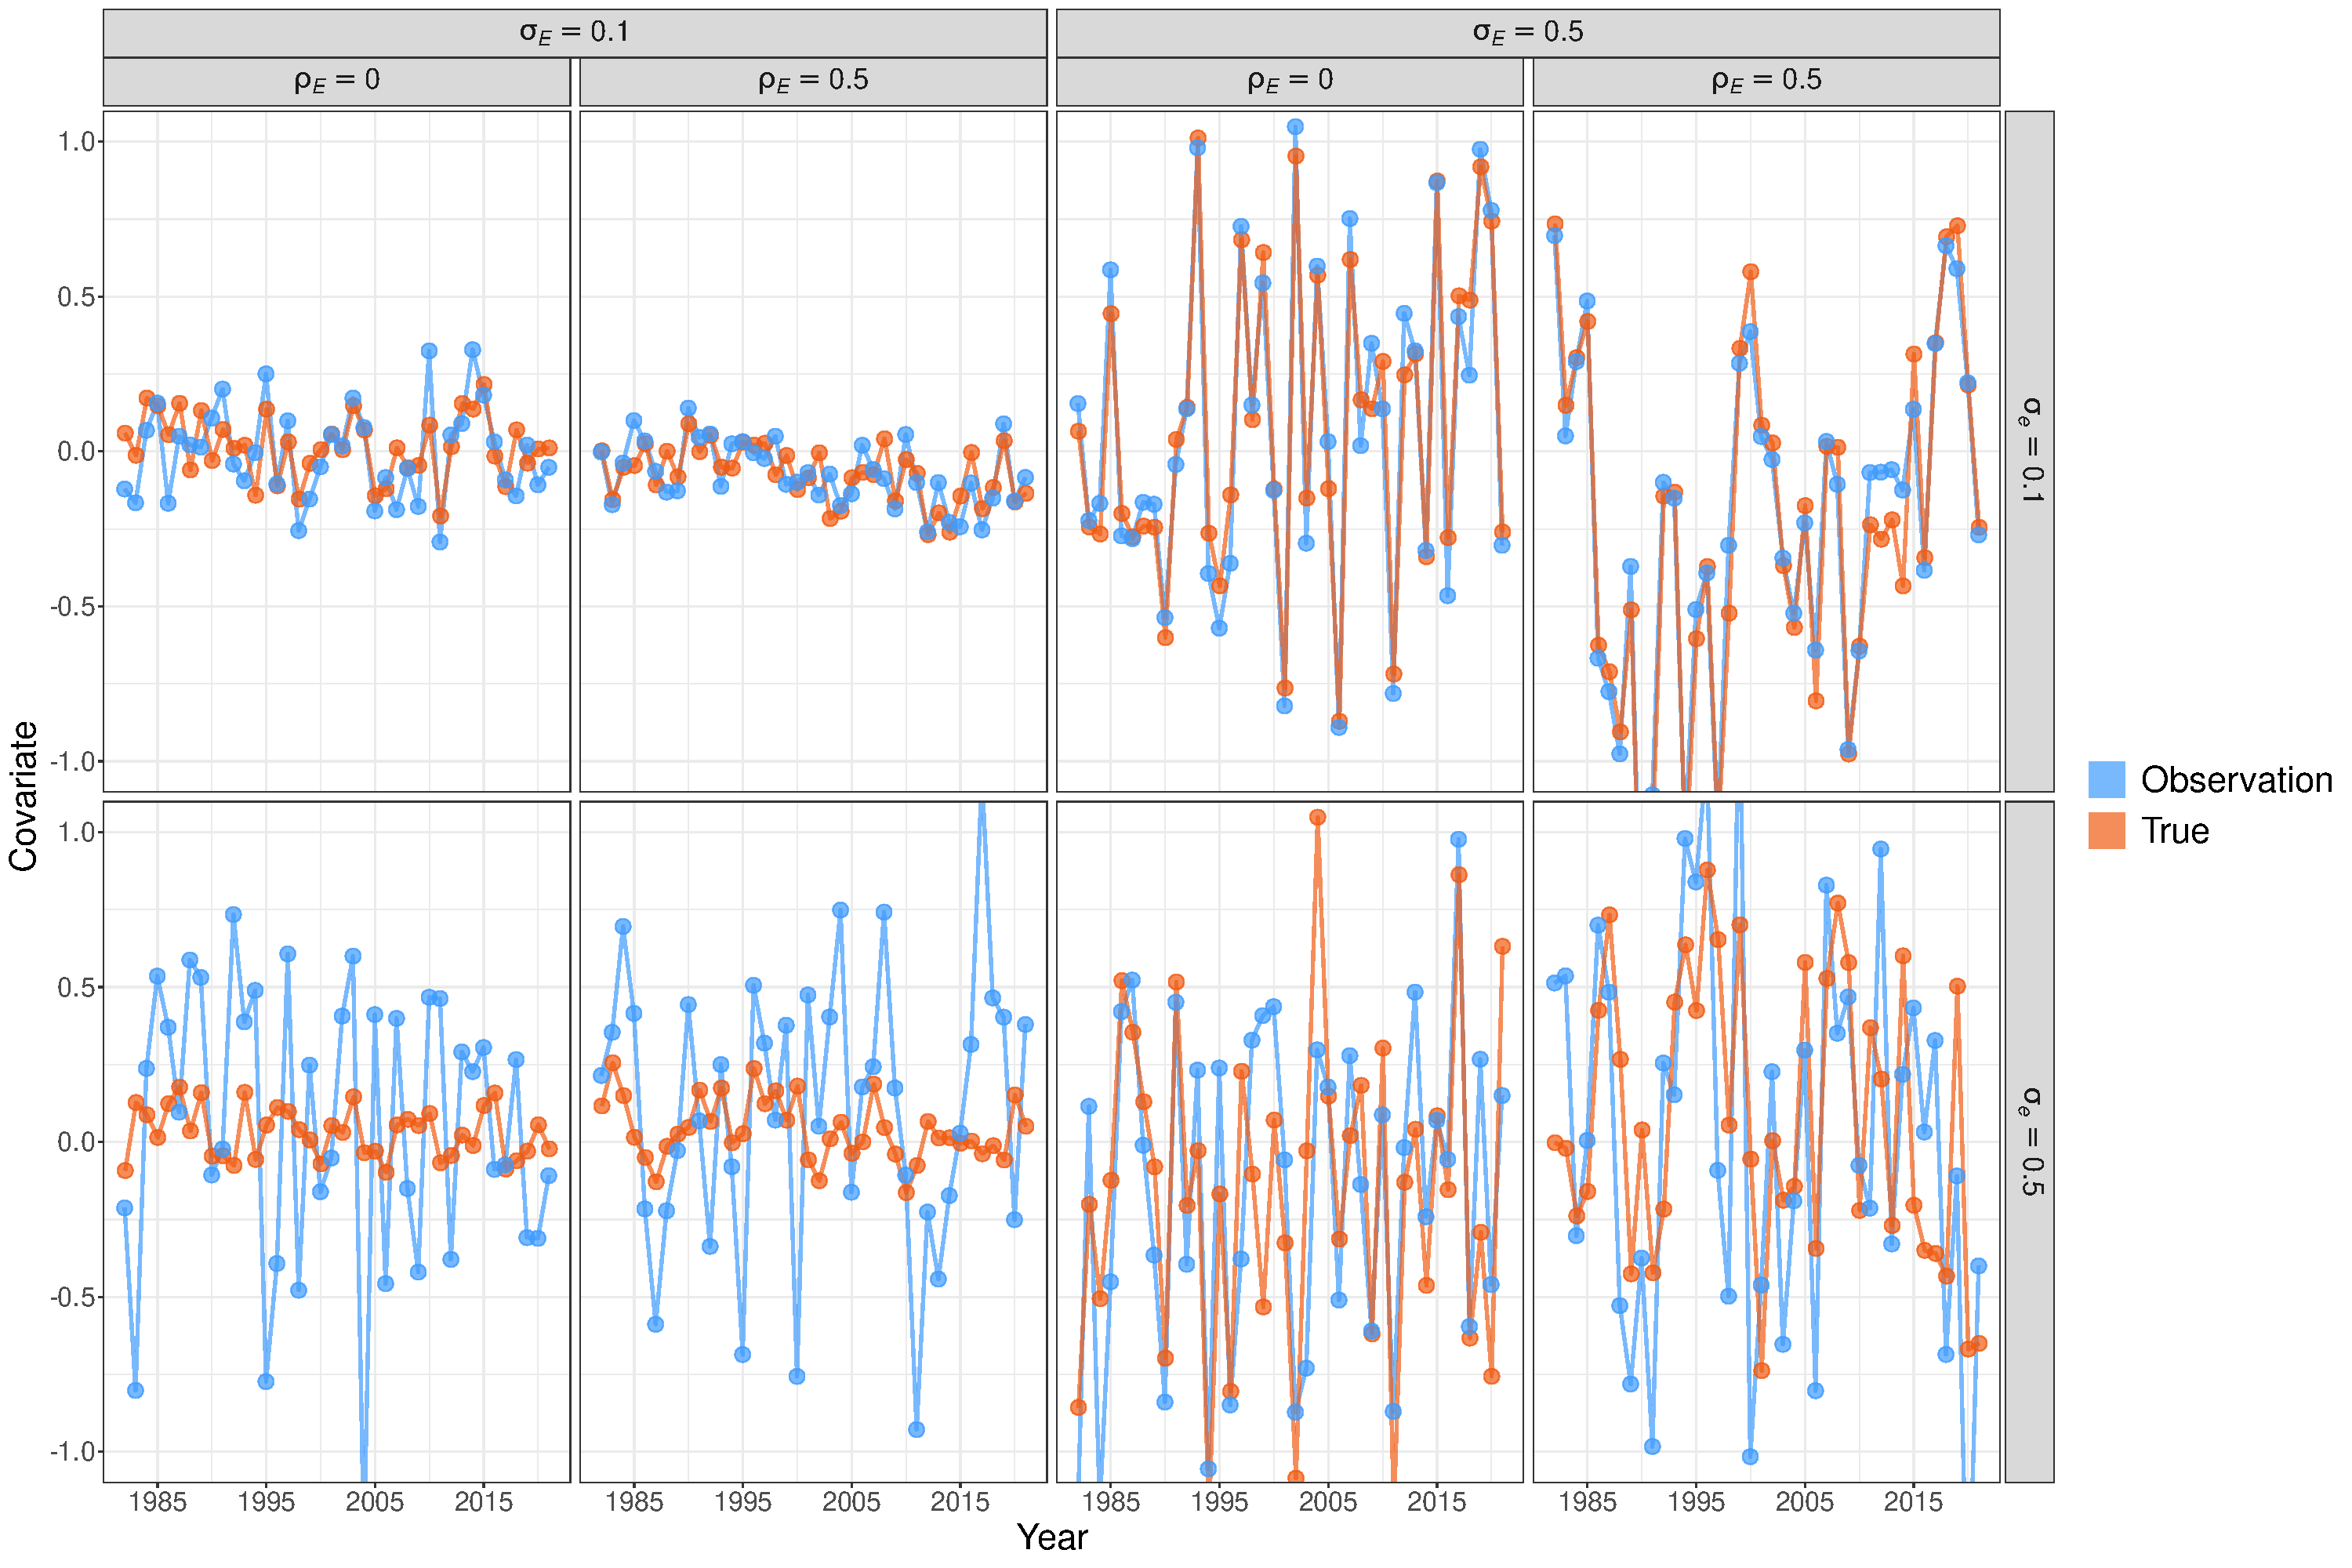
\includegraphics[height = \textheight]{Ecov_true_obs_example}
\end{center}
\caption{\DIFaddFL{Example simulations of environmental covariate latent processes and observations with different levels of observation error, and different assumptions about variability of the latent process.}}\label{om_ecov_example}
\end{figure}
\end{landscape}

\begin{figure}
\begin{center}
\DIFaddendFL 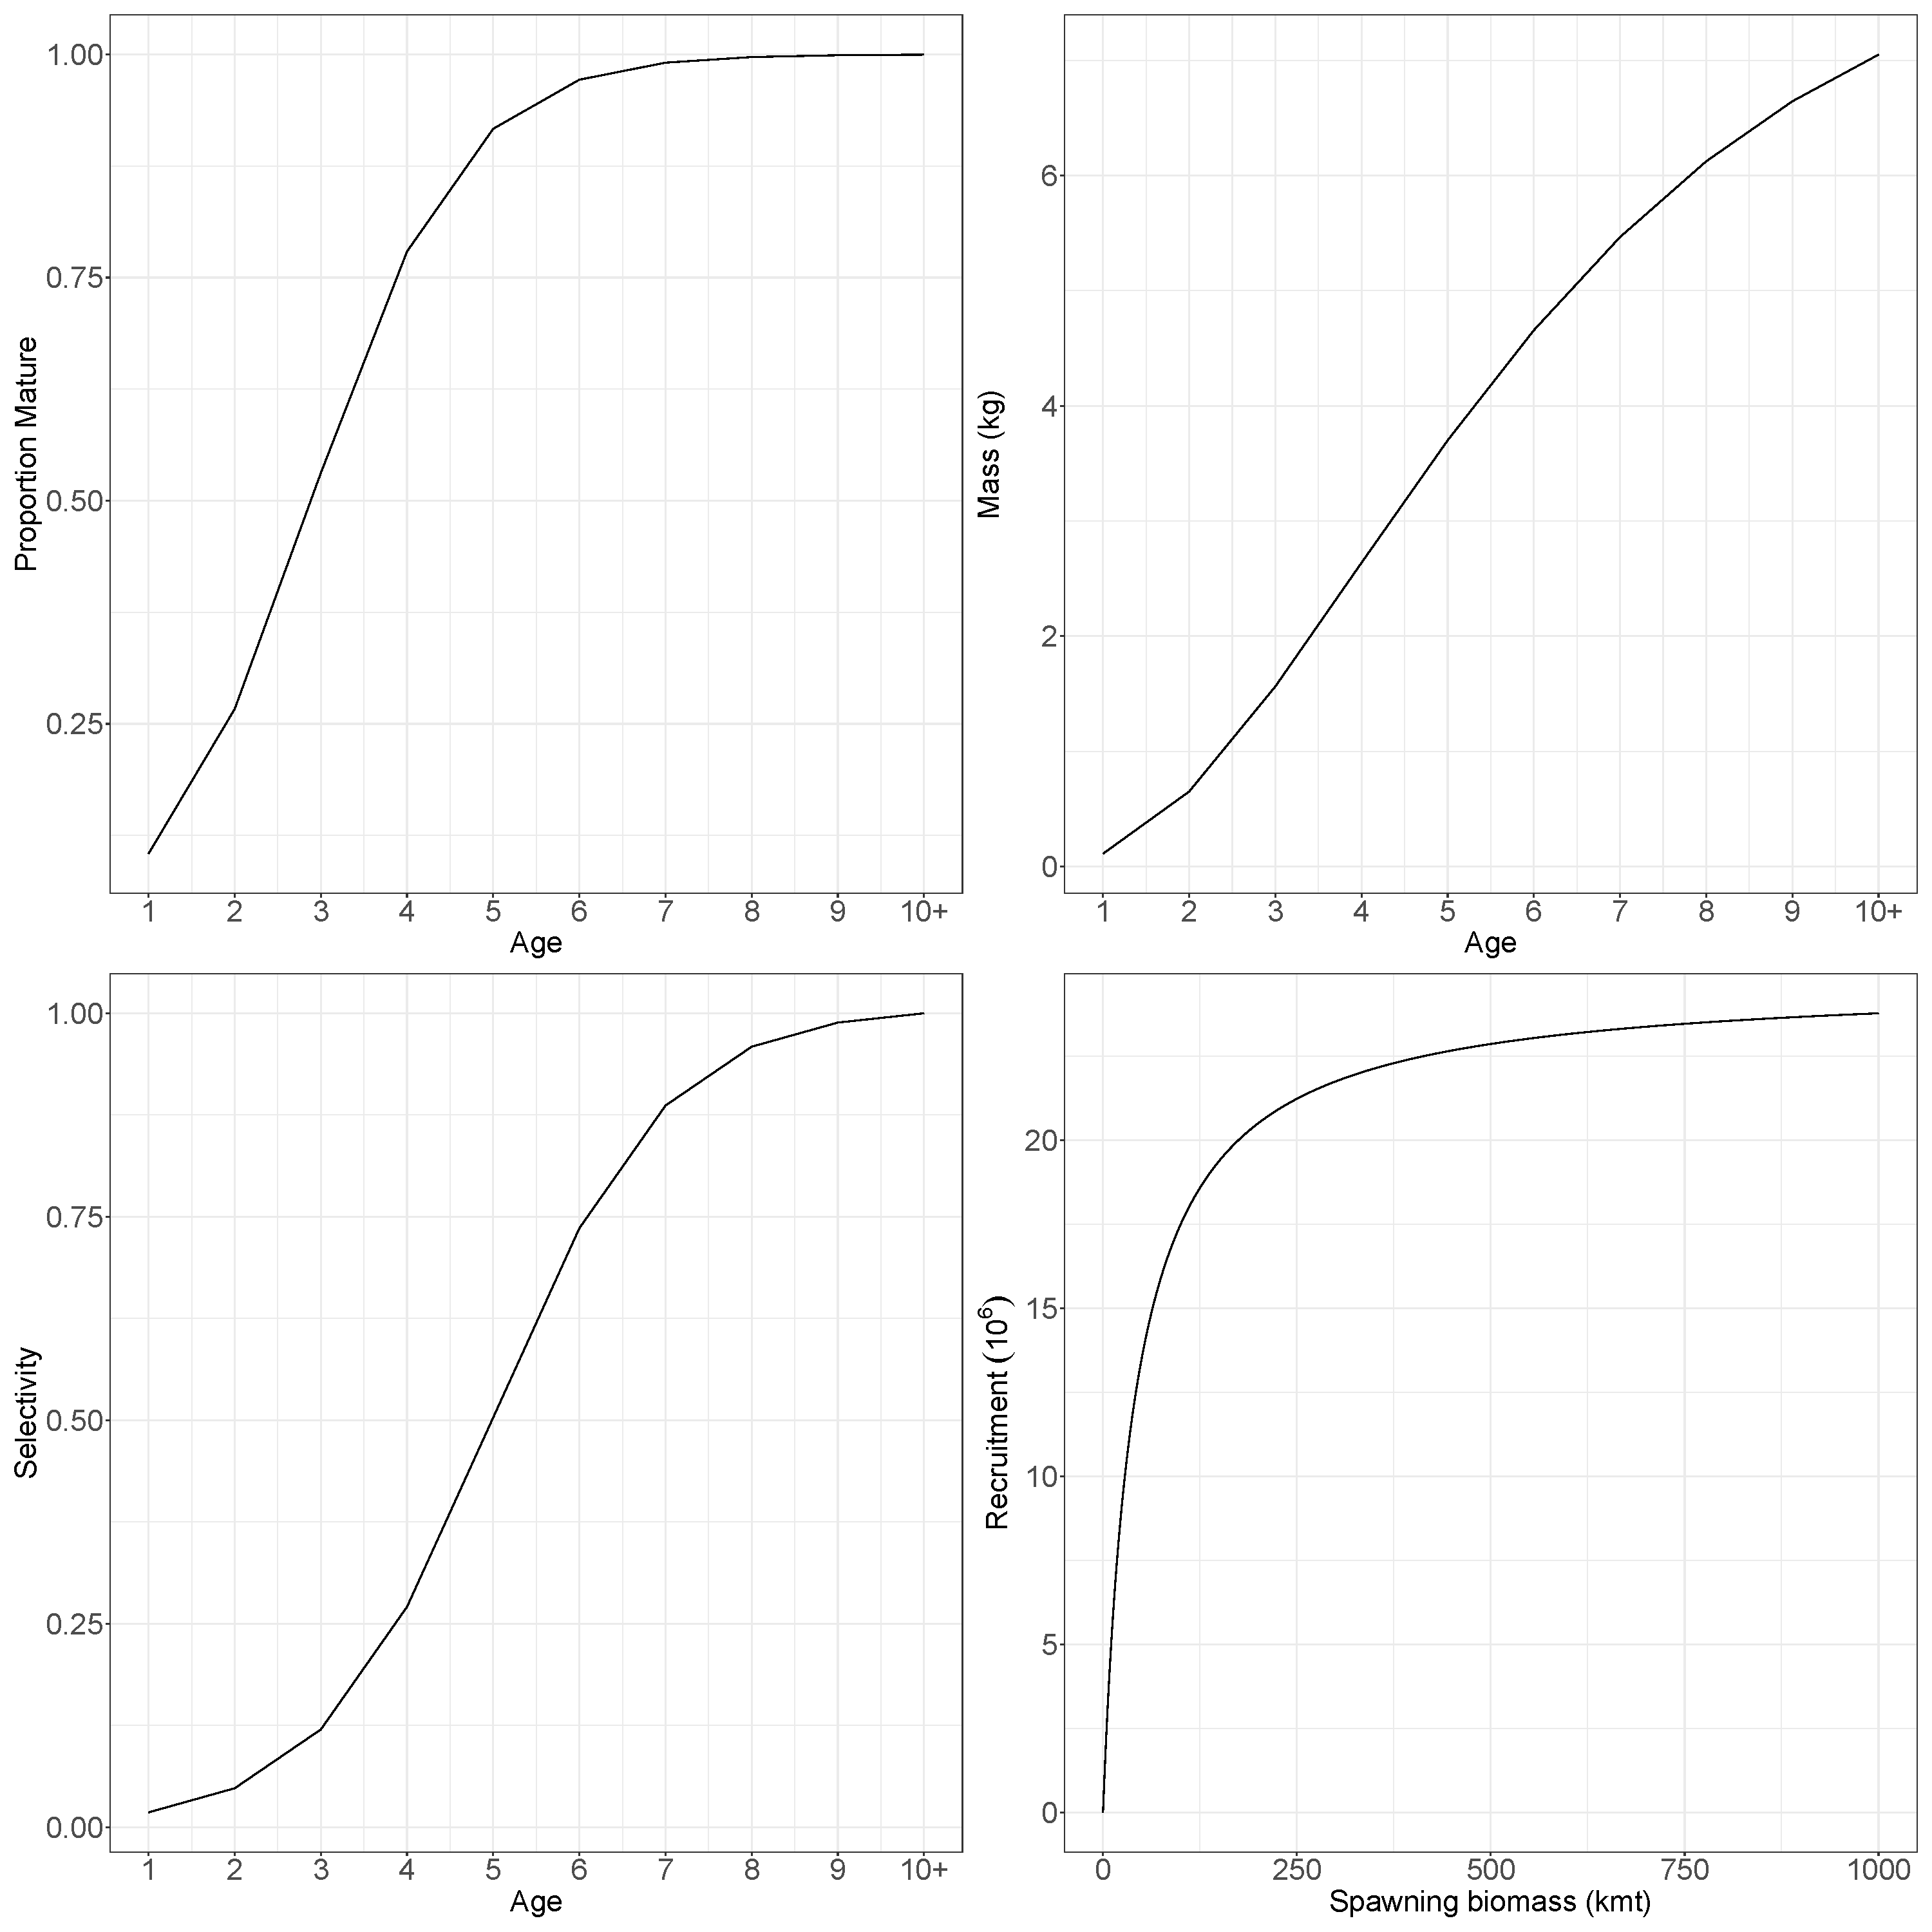
\includegraphics[width = \textwidth]{om_input_plots_figure}
\end{center}
\caption{The proportion mature at age, weight at age, fleet and index selectivity at age, and Beverton-Holt stock-recruit relationship assumed for the population in all \DIFdelbeginFL \DIFdelFL{operating models}\DIFdelendFL \DIFaddbeginFL \DIFaddFL{OMs}\DIFaddendFL . For \DIFdelbeginFL \DIFdelFL{operating models }\DIFdelendFL \DIFaddbeginFL \DIFaddFL{OMs }\DIFaddendFL with random effects on fleet selectivity, this represents the selectivity at the mean of the random effects.}\label{om_inputs_fig}
\end{figure}

\begin{landscape}
\begin{figure}
\DIFdelbeginFL %DIFDELCMD < \caption{%
{%DIFAUXCMD
\DIFdelFL{Example simulations of environmental covariate latent processes and observations with different levels of observation error, and different assumptions about variability of the latent process.}}%DIFAUXCMD
%DIFDELCMD < \label{om_ecov_example}
%DIFDELCMD < %%%
\DIFdelendFL \begin{center}
\DIFdelbeginFL %DIFDELCMD < 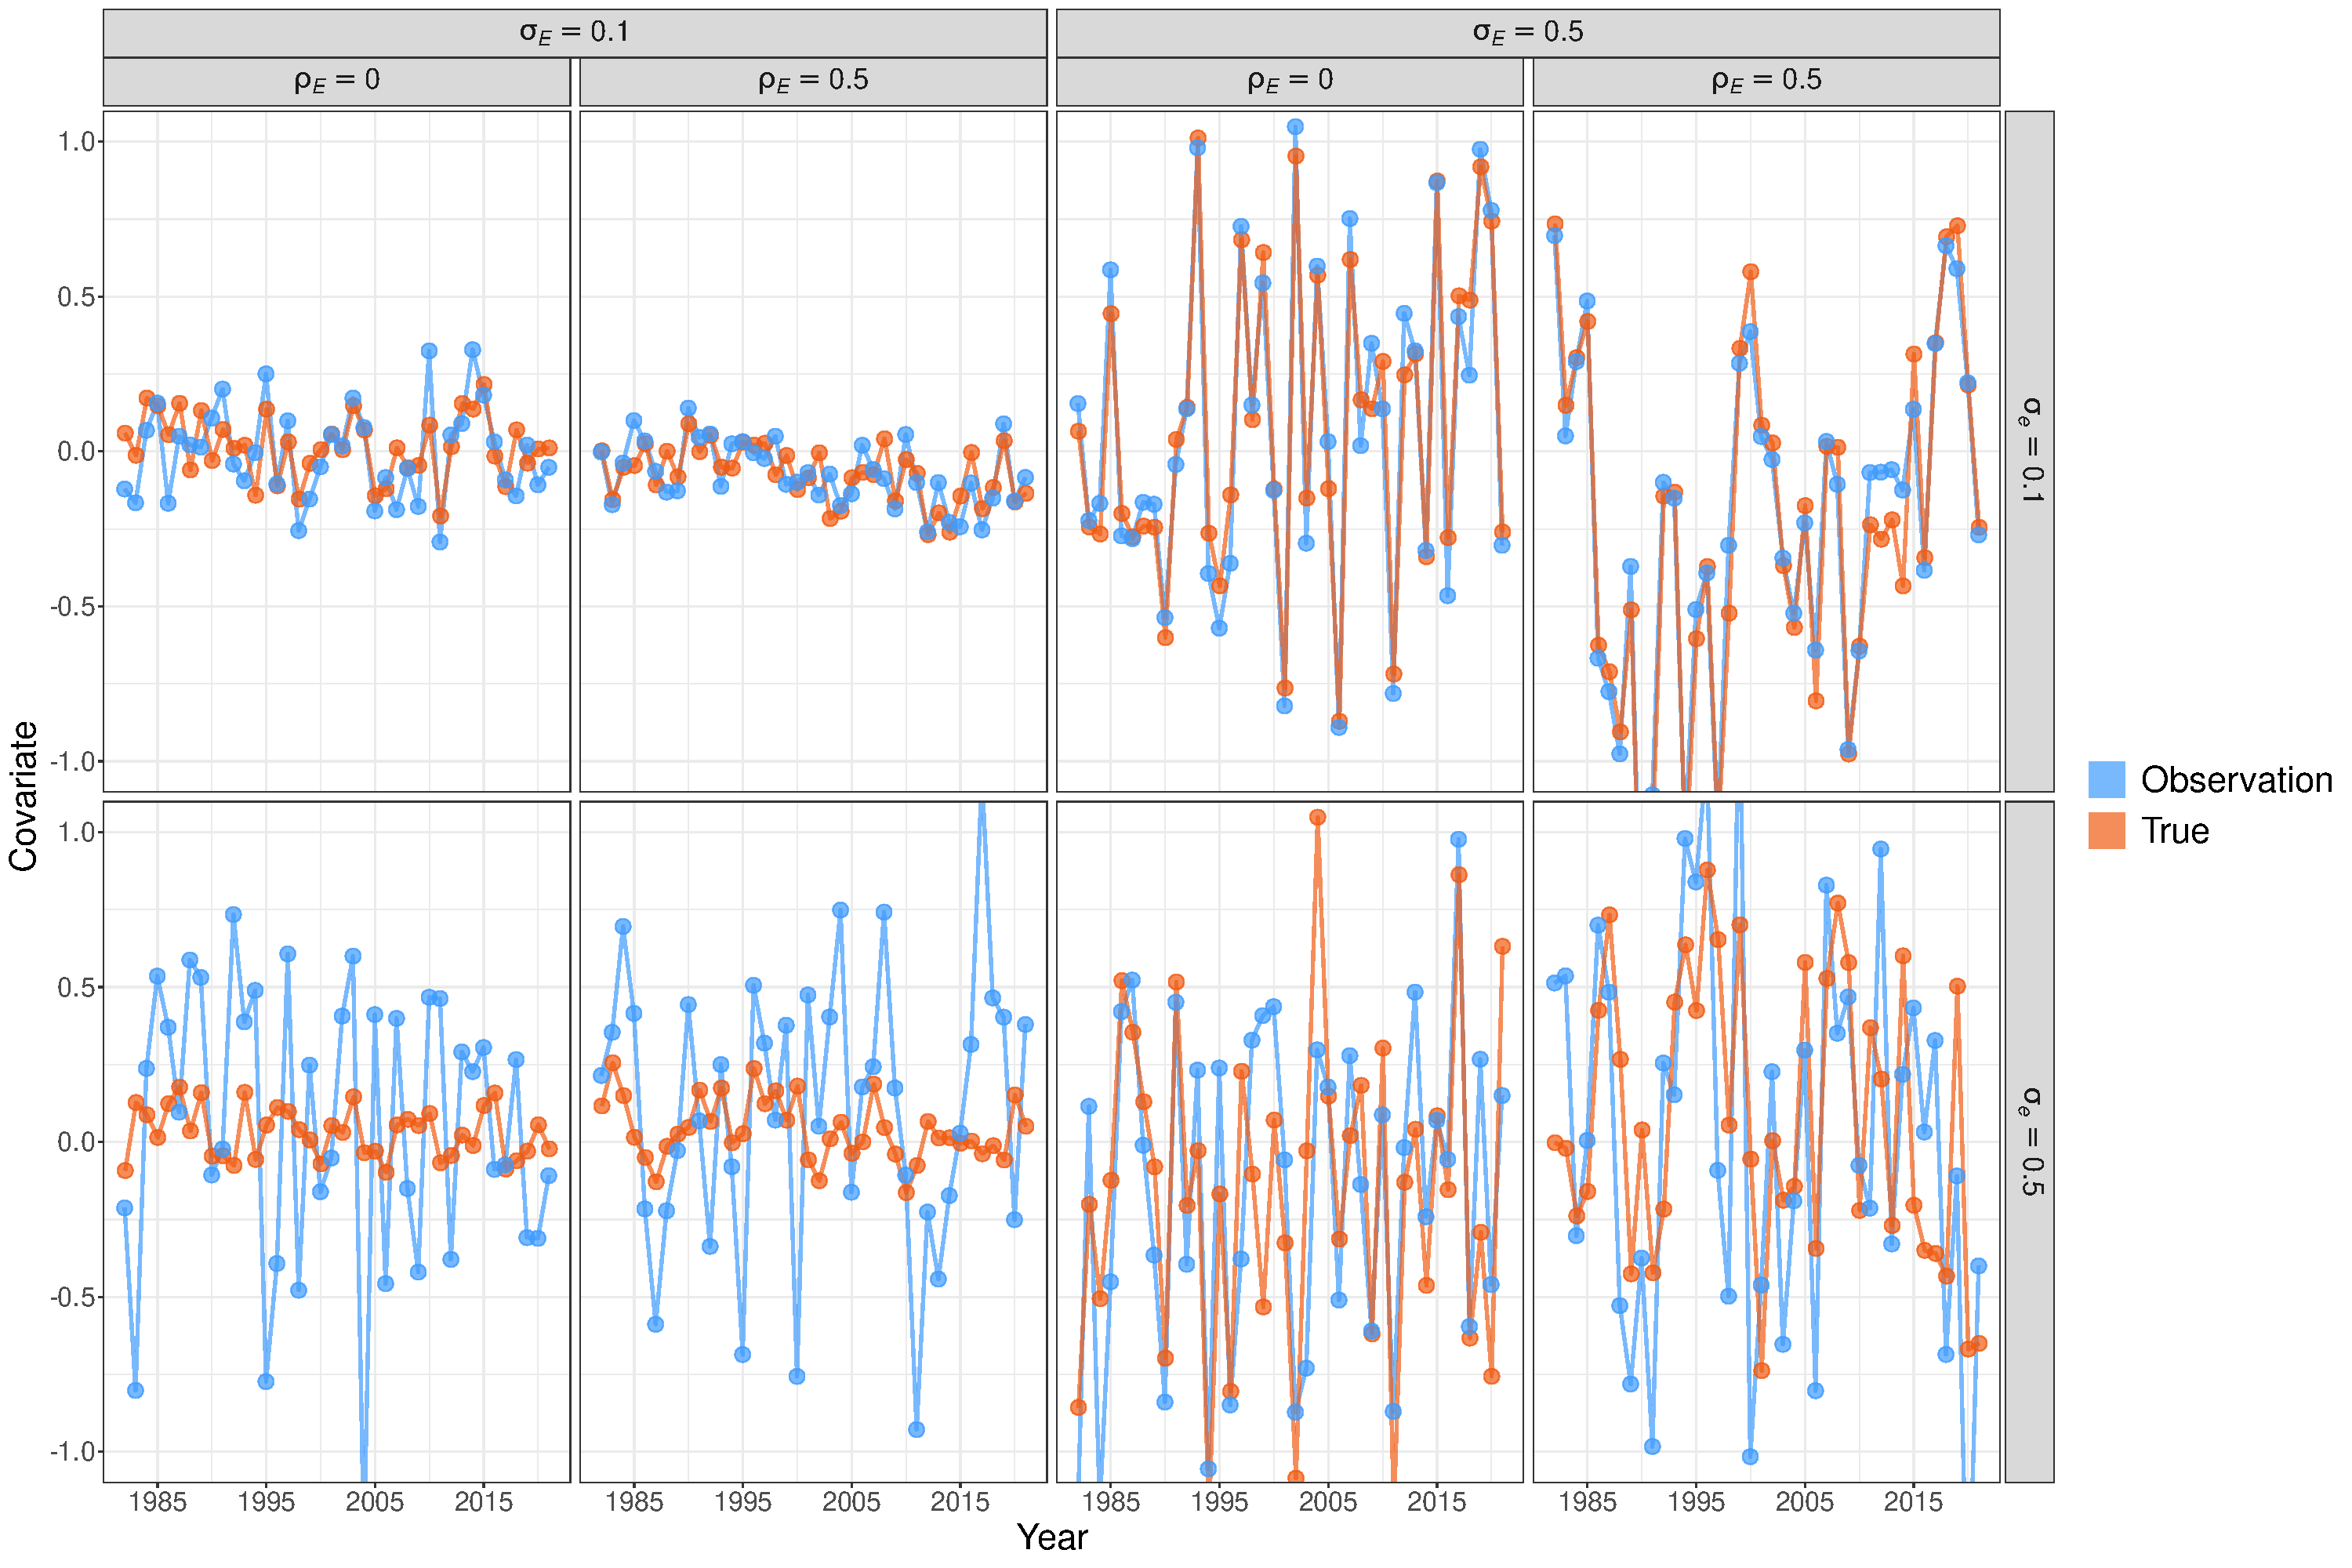
\includegraphics[height = \textheight]{Ecov_true_obs_example}
%DIFDELCMD < %%%
\DIFdelendFL \DIFaddbeginFL 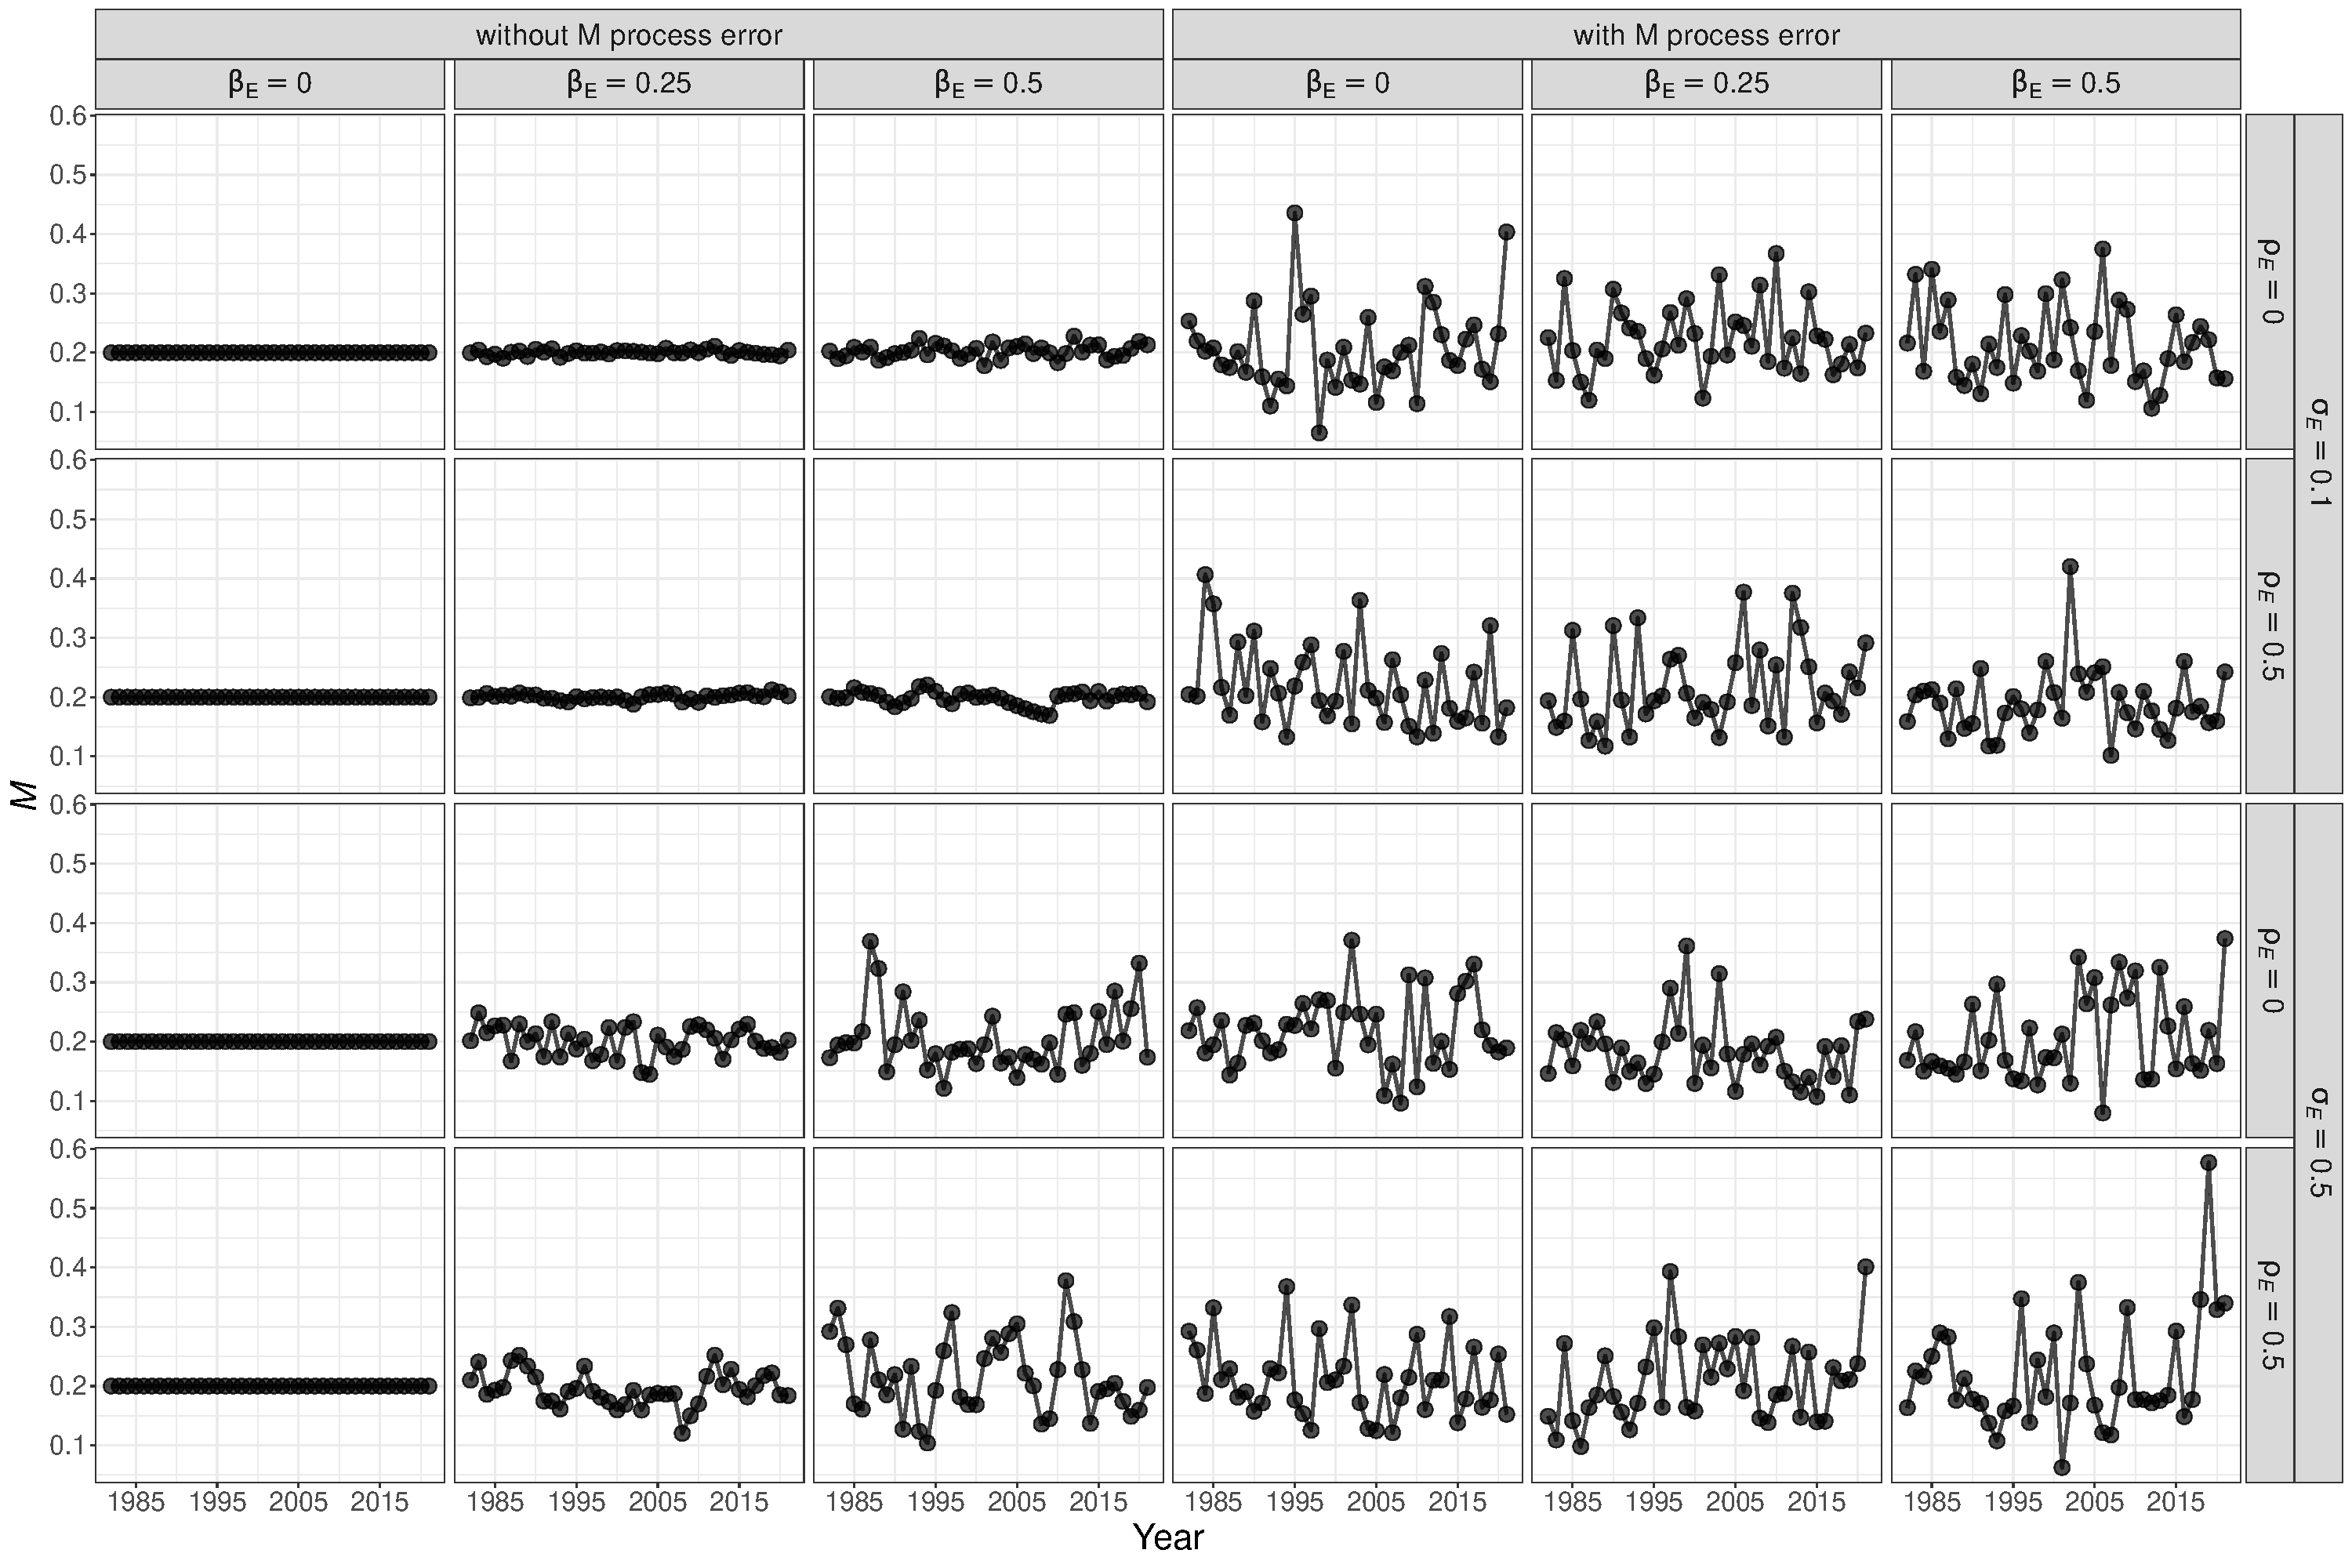
\includegraphics[height = \textheight]{M_example}
\DIFaddendFL \end{center}
\DIFaddbeginFL \caption{\DIFaddFL{Example simulations of annual $M$ that may be a function of a temporally varying environmental covariate and autoregressive random effects.}}\label{M_example}
\DIFaddendFL \end{figure}
\end{landscape}

\begin{landscape}
\begin{figure}
\DIFdelbeginFL %DIFDELCMD < \caption{%
{%DIFAUXCMD
\DIFdelFL{Example simulations of annual natural mortality rates that may be a function of a temporally varying environmental covariate and autoregressive random effects.}}%DIFAUXCMD
%DIFDELCMD < \label{M_example}
%DIFDELCMD < %%%
\DIFdelendFL \begin{center}
\DIFdelbeginFL %DIFDELCMD < 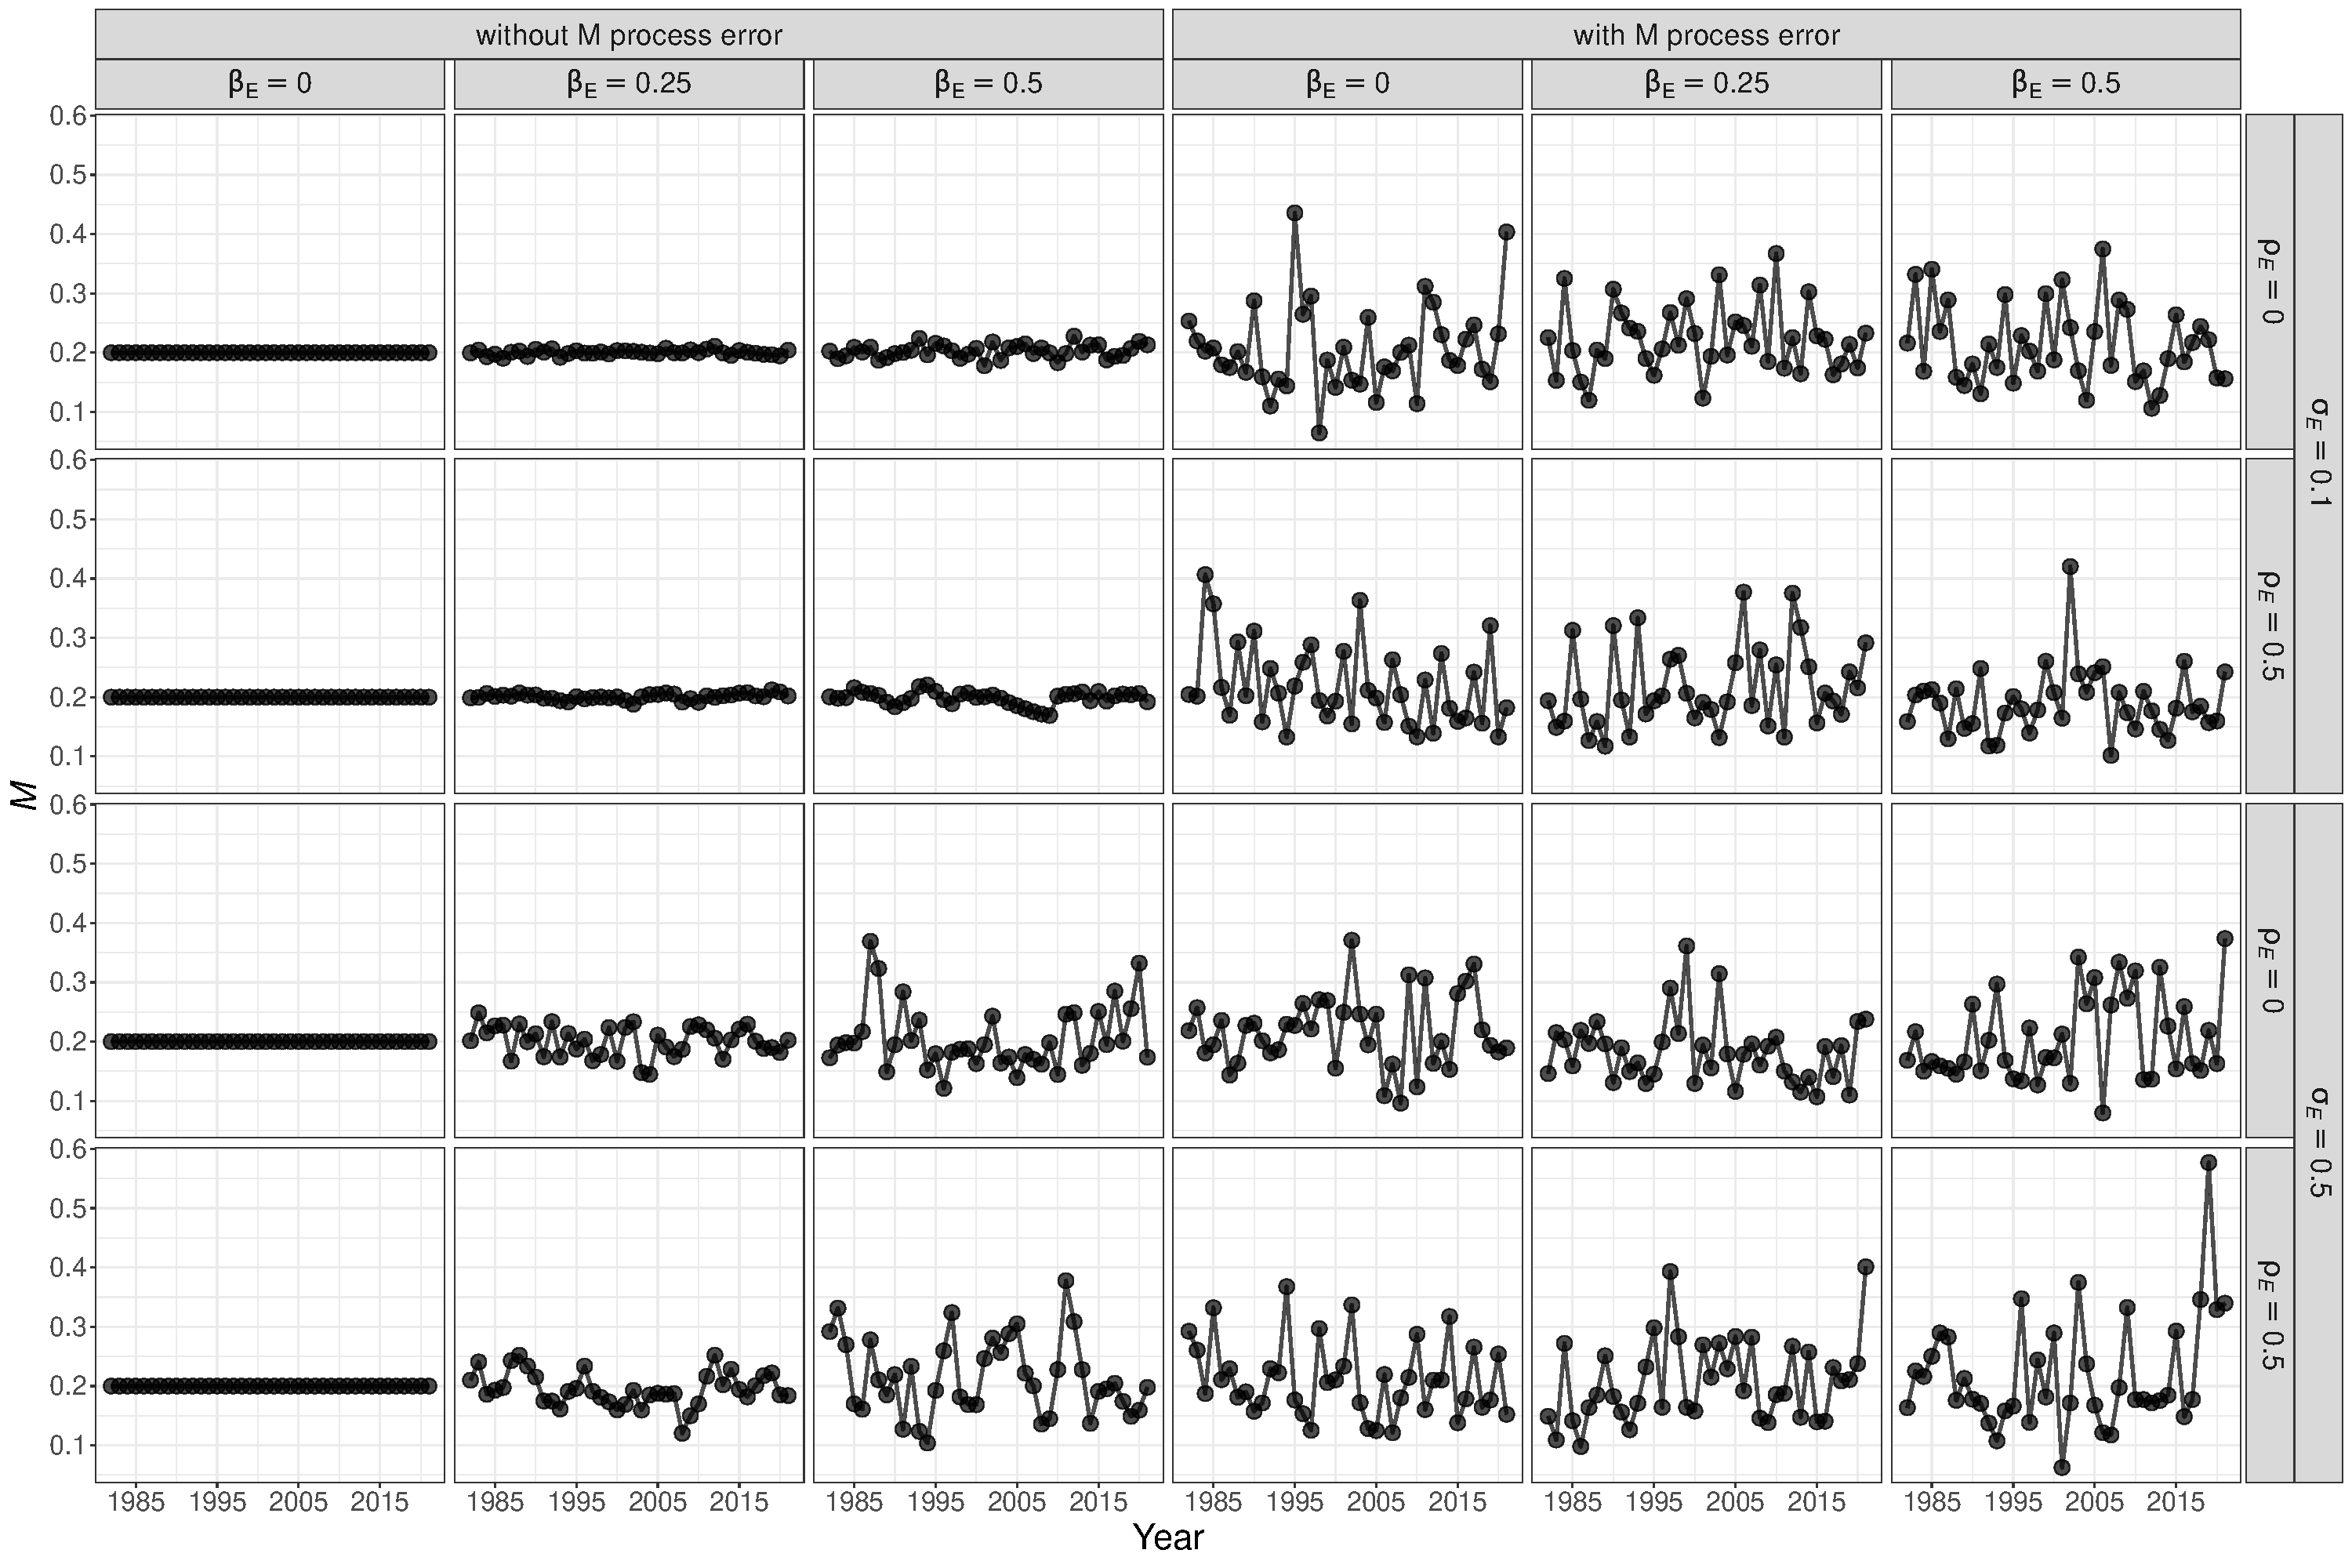
\includegraphics[height = \textheight]{M_example}
%DIFDELCMD < %%%
\DIFdelendFL \DIFaddbeginFL 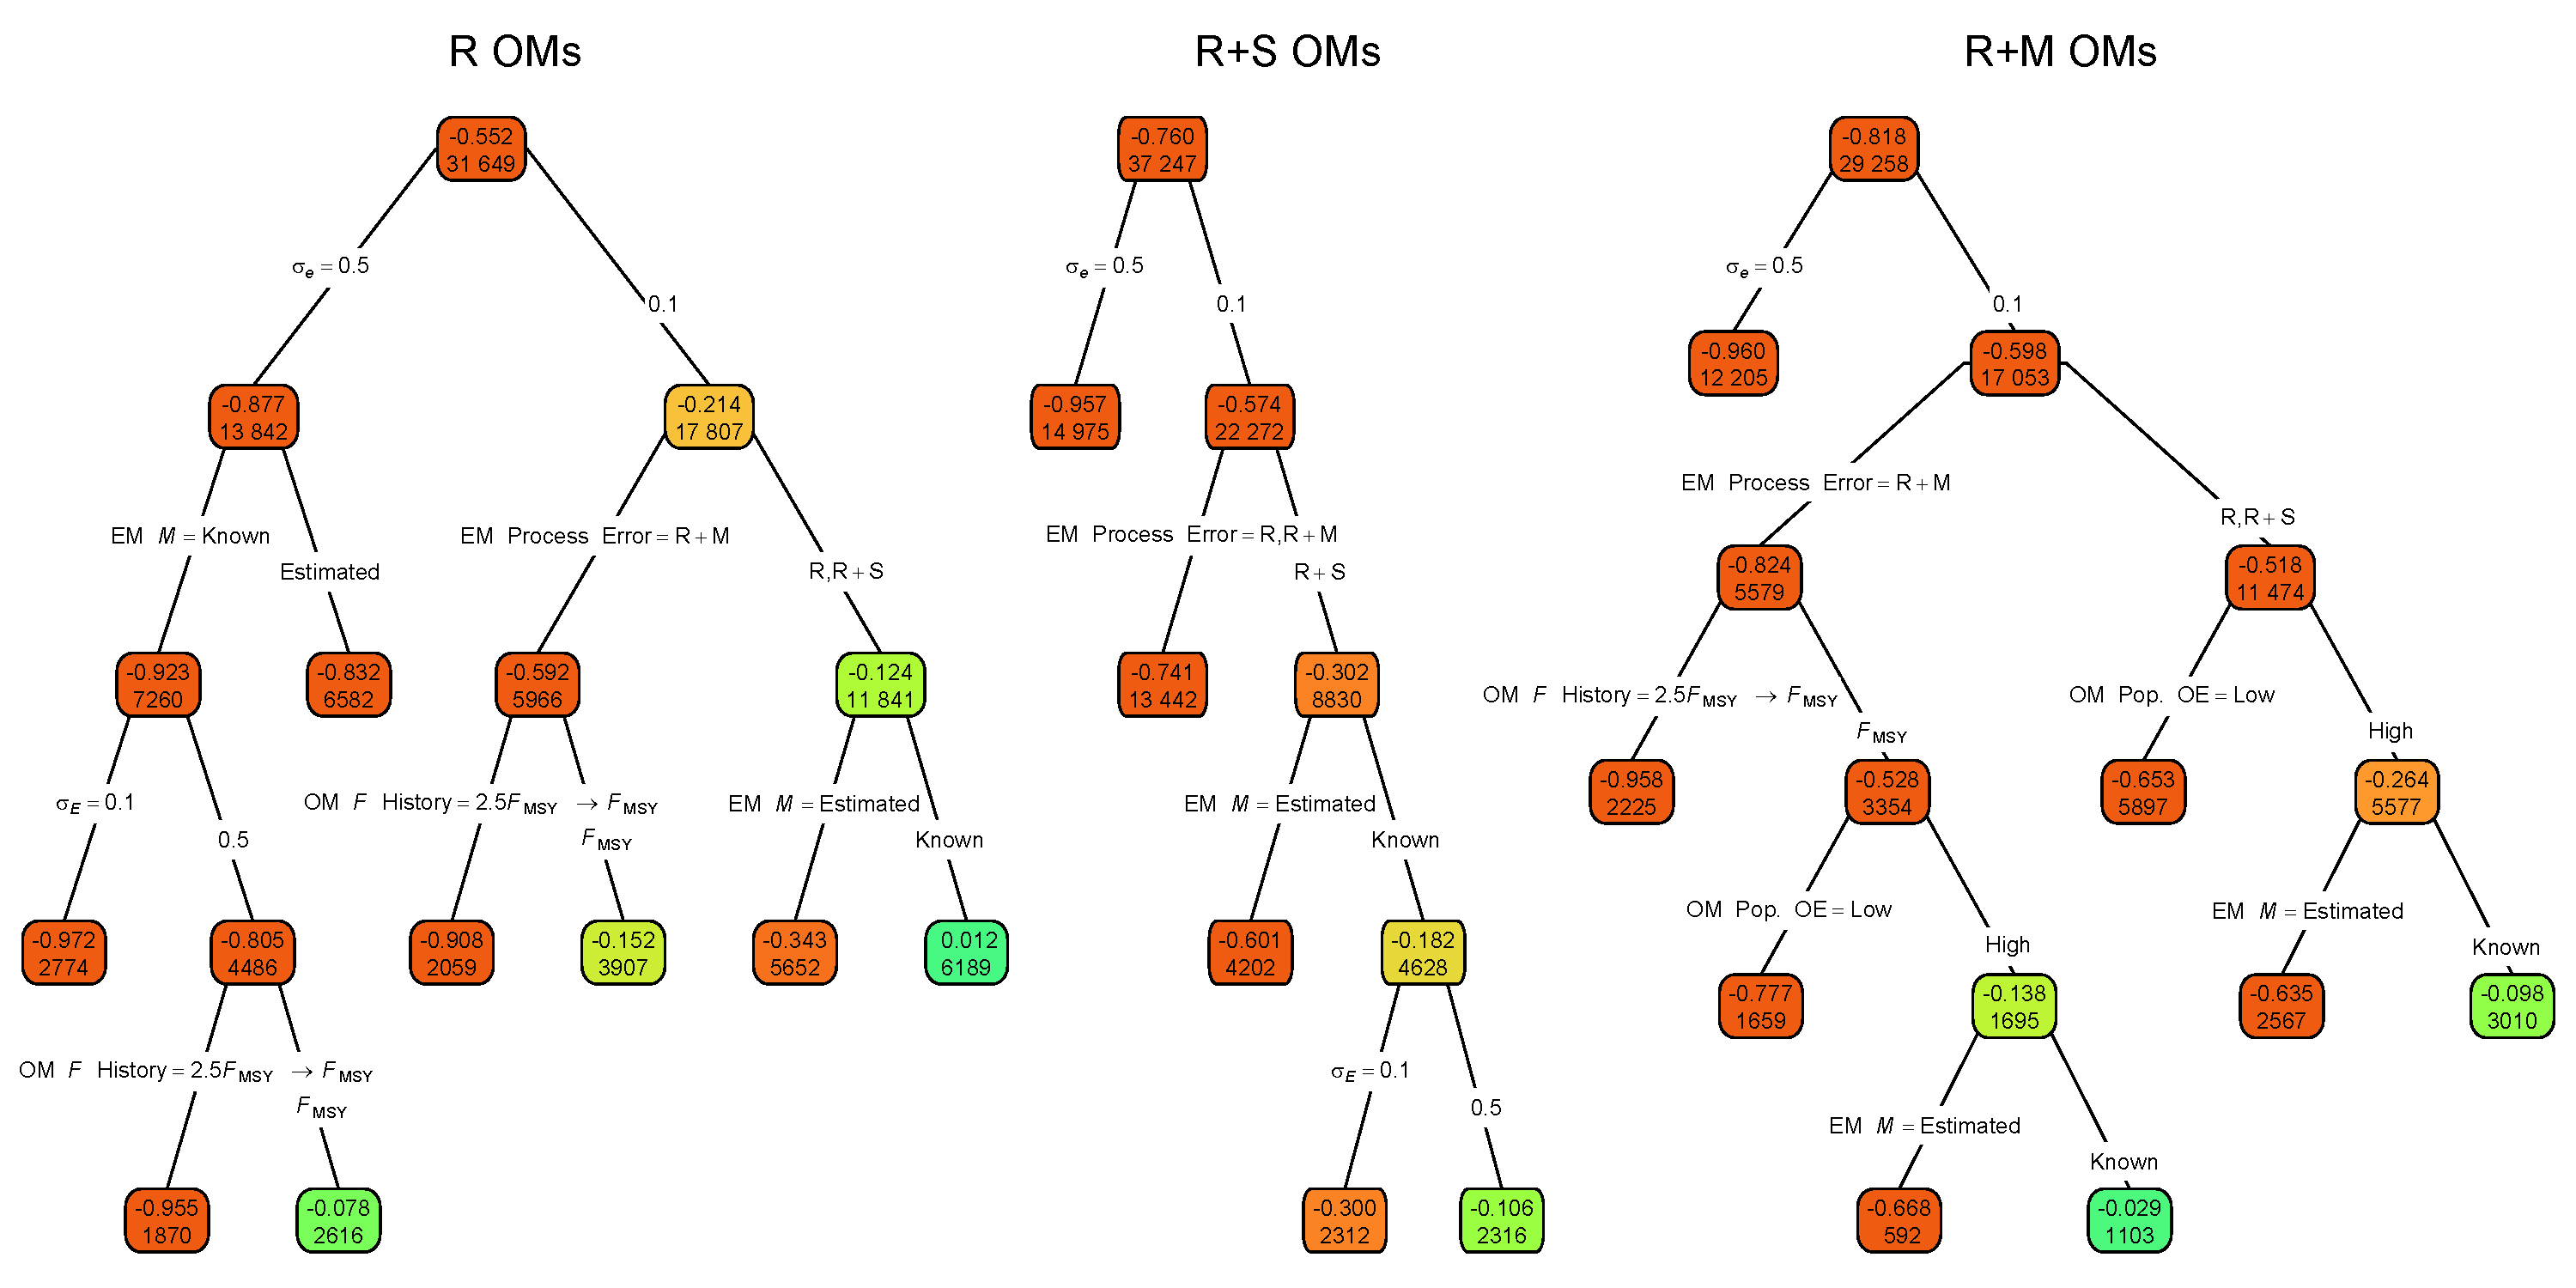
\includegraphics[width = 1.4\textwidth]{ecov_beta_SE_bias_regtree_plots}
\DIFaddendFL \end{center}
\DIFaddbeginFL \caption{\DIFaddFL{Regression trees indicating primary factors determining reductions in sums of squares of errors in estimation of the Hessian-based standard error estimates for covariate effect on $M$ ($\widehat {\text{SE}}\left(\widehat \beta_E\right)$) for operating models (OMs) with process error on recruitment only (R), recruitment and apparent survival (R+S), or recruitment and natural mortality (R+M). Each node shows the median error (top) and number of observations (bottom) for the corresponding subset. Lower or higher median absolute errors of the process error assumption are indicated by more green or red polygons, respectively.}}\label{ecov_effect_SE_bias_regtree}
\DIFaddendFL \end{figure}
\end{landscape}

\DIFdelbegin %DIFDELCMD < \hypertarget{convergence-results}{%
%DIFDELCMD < \subsection*{Convergence results}\label{convergence-results}}
%DIFDELCMD < %%%
\DIFdelend \DIFaddbegin \begin{landscape}
\begin{figure}
\begin{center}
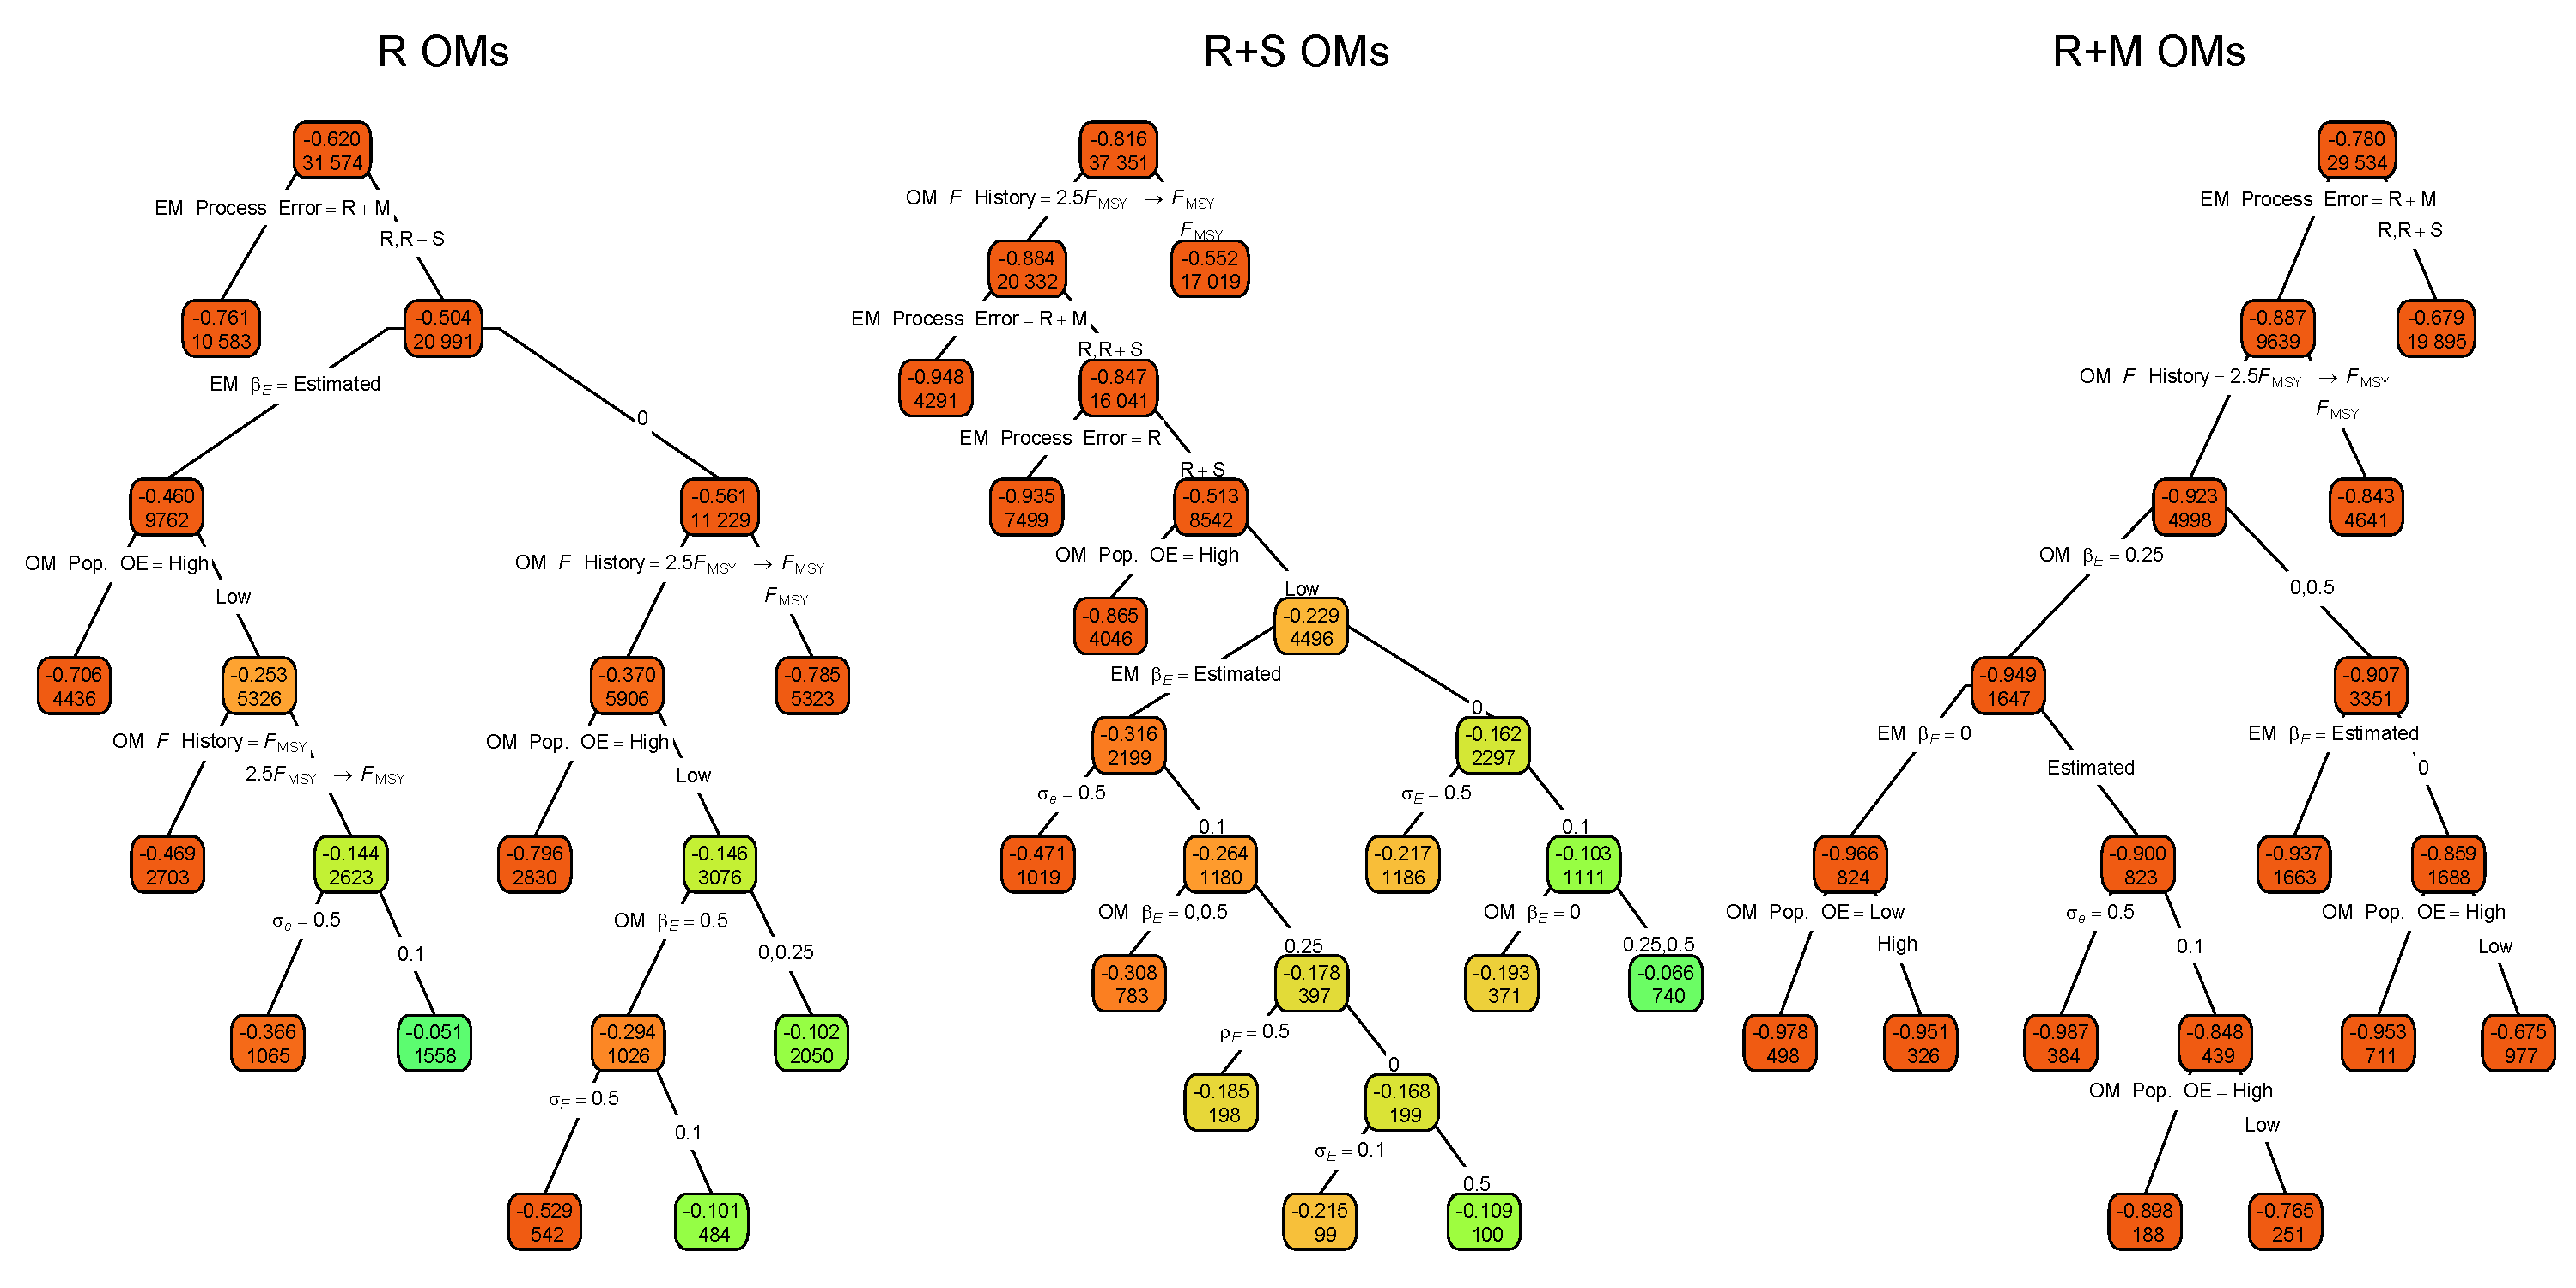
\includegraphics[width = 1.4\textwidth]{median_M_SE_bias_regtree_plots}
\end{center}
\caption{\DIFaddFL{Regression trees indicating primary factors determining reductions in sums of squares of errors in estimation of the Hessian-based standard error estimates for median $M$ parameter ($\widehat {\text{SE}}\left(\widehat \beta_M\right)$) in EMs fitted to operating models (OMs) with process error on recruitment only (R), recruitment and apparent survival (R+S), or recruitment and natural mortality (R+M). Each node shows the median error (top) and number of observations (bottom) for the corresponding subset. Lower or higher median absolute errors of the process error assumption are indicated by more green or red polygons, respectively.}}\label{med_M_SE_bias_regtree}
\end{figure}
\end{landscape}

\begin{landscape}
\begin{figure}
\begin{center}
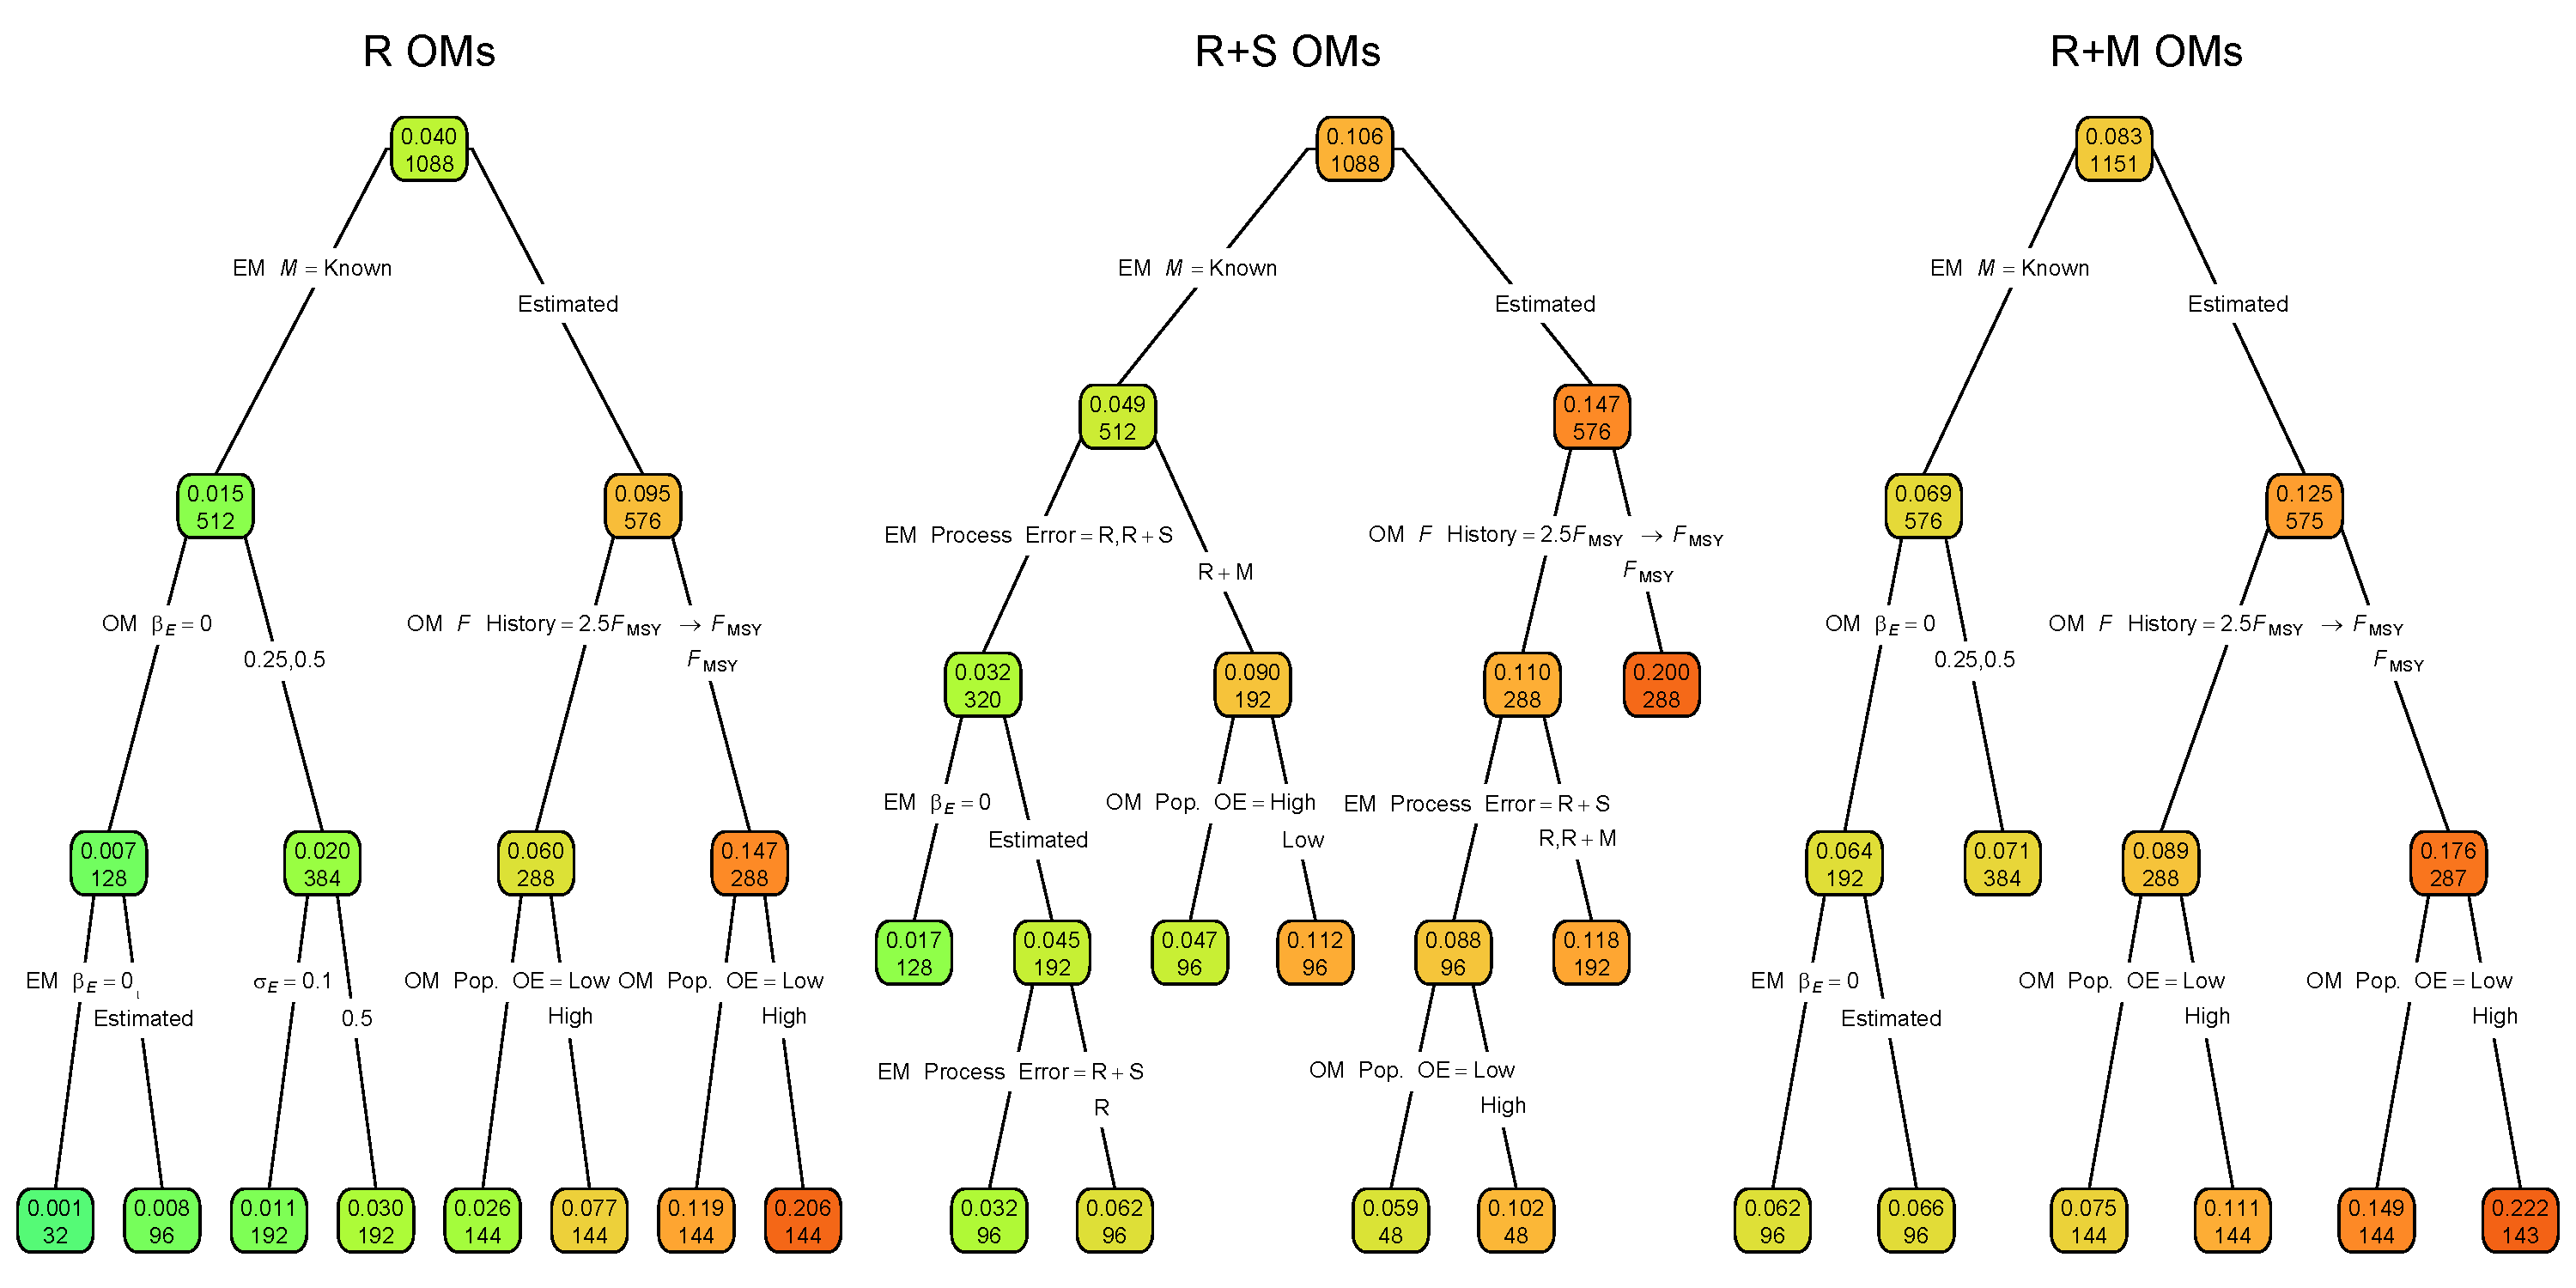
\includegraphics[width = 1.4\textwidth]{term_M_rmse_regtree_plots}
\end{center}
\caption{\DIFaddFL{Regression trees indicating primary factors determining reductions in sums of squares for the log-transformed RMSE of terminal year $M$ in EMs fitted to operating models (OMs) with process error on recruitment only (R), recruitment and apparent survival (R+S), or recruitment and natural mortality (R+M). Each node shows the median error (top) and number of observations (bottom) for the corresponding subset. Lower or higher median RMSE are indicated by more red or green polygons, respectively.}}\label{term_M_rmse_regtree}
\end{figure}
\end{landscape}

\begin{landscape}
\begin{figure}
\begin{center}
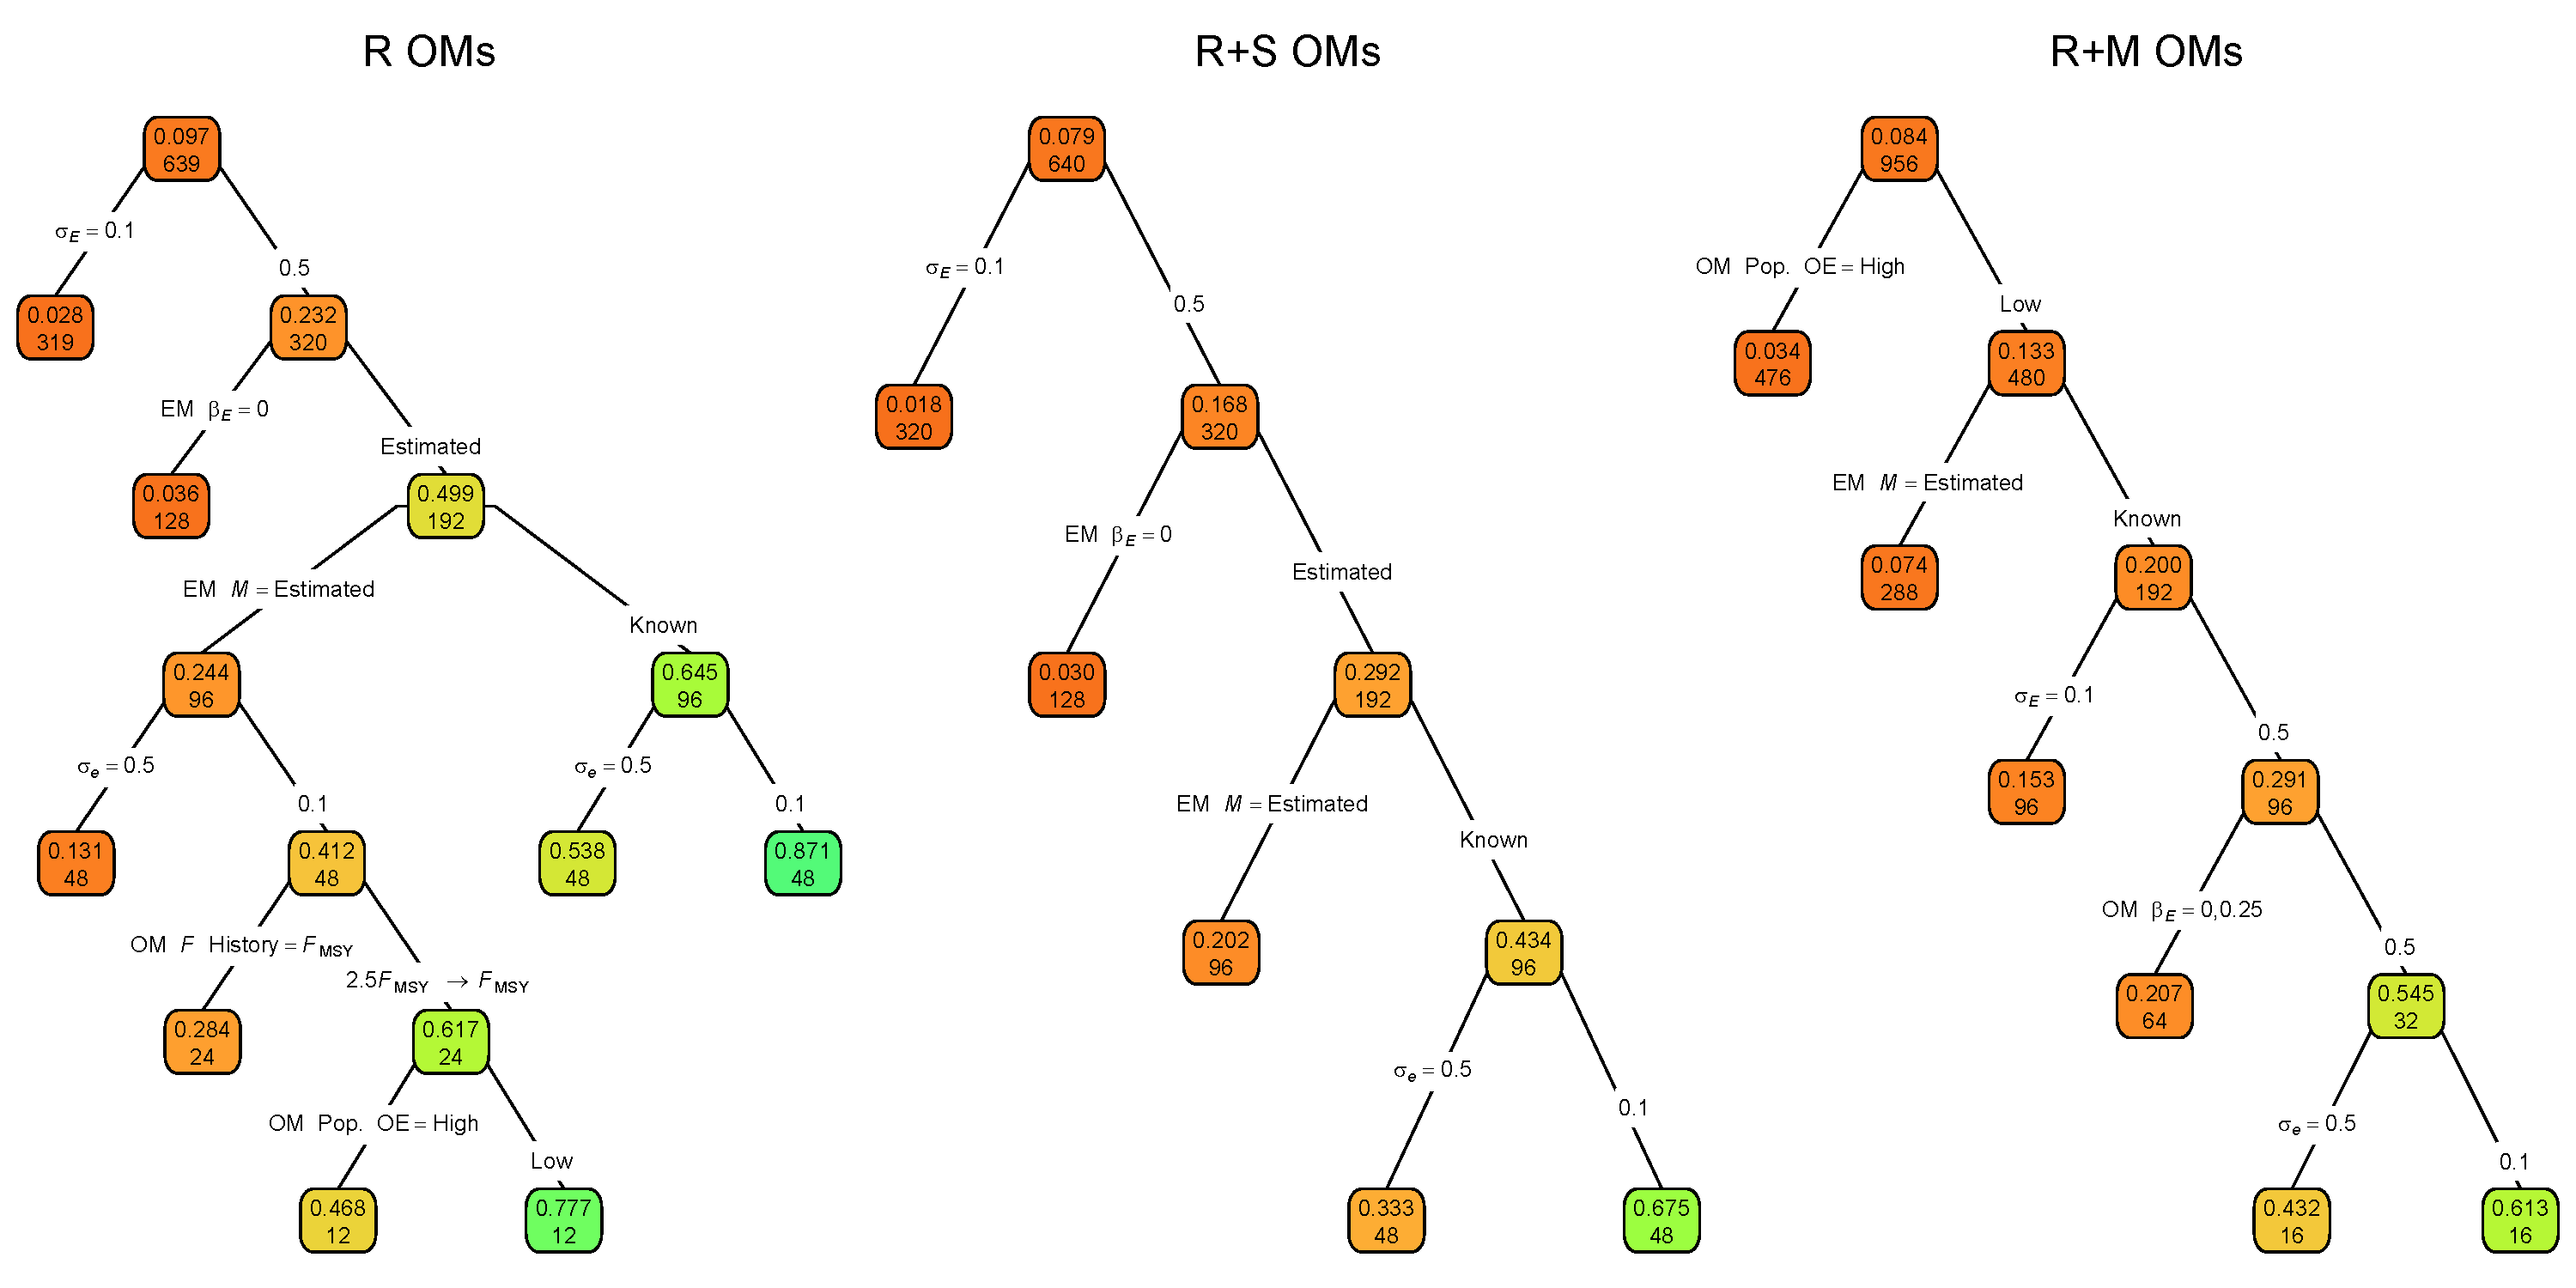
\includegraphics[width = 1.4\textwidth]{term_M_corr_regtree_plots}
\end{center}
\caption{\DIFaddFL{Regression trees indicating primary factors determining reductions in sums of squares for the correlation of terminal year $M$ estimates and true values in EMs fitted to operating models (OMs) with process error on recruitment only (R), recruitment and apparent survival (R+S), or recruitment and natural mortality (R+M). Each node shows the median error (top) and number of observations (bottom) for the corresponding subset. Lower or higher median correlations are indicated by more red or green polygons, respectively.}}\label{term_M_corr_regtree}
\end{figure}
\end{landscape}

\begin{landscape}
\begin{figure}
\begin{center}
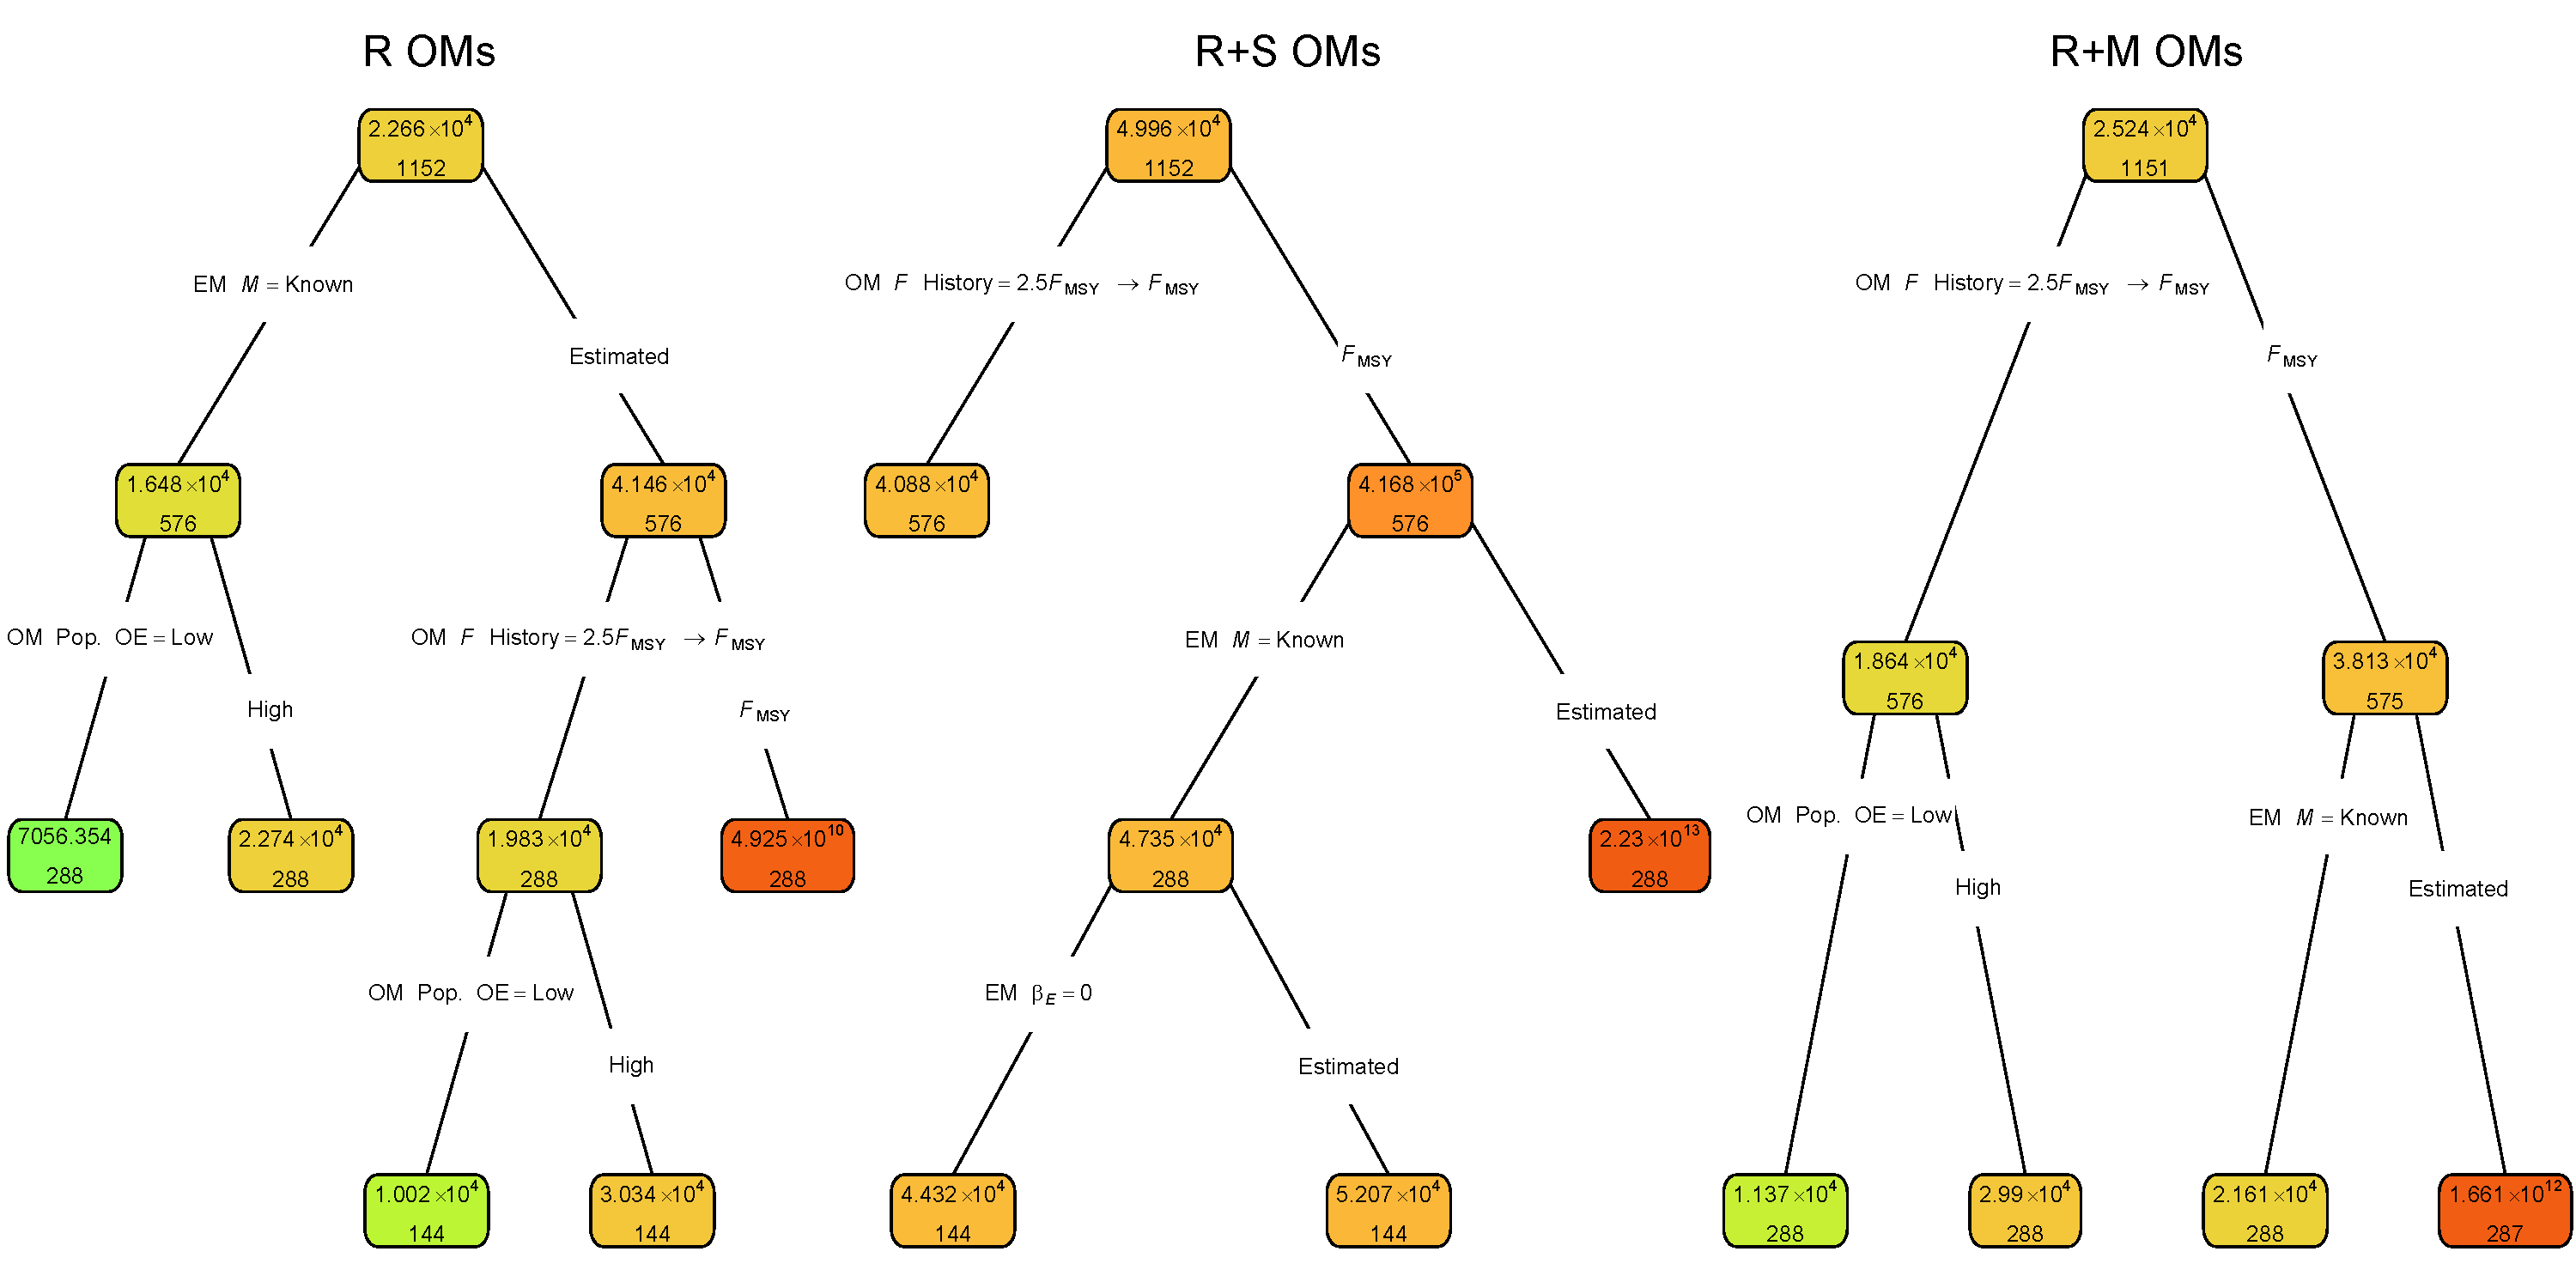
\includegraphics[width = 1.4\textwidth]{term_SSB_rmse_regtree_plots}
\end{center}
\caption{\DIFaddFL{Regression trees indicating primary factors determining reductions in sums of squares for the log-transformed RMSE of terminal year SSB in EMs fitted to operating models (OMs) with process error on recruitment only (R), recruitment and apparent survival (R+S), or recruitment and natural mortality (R+M). Each node shows the median error (top) and number of observations (bottom) for the corresponding subset. Lower or higher median RMSE are indicated by more red or green polygons, respectively.}}\label{term_SSB_rmse_regtree}
\end{figure}
\end{landscape}

\begin{landscape}
\begin{figure}
\begin{center}
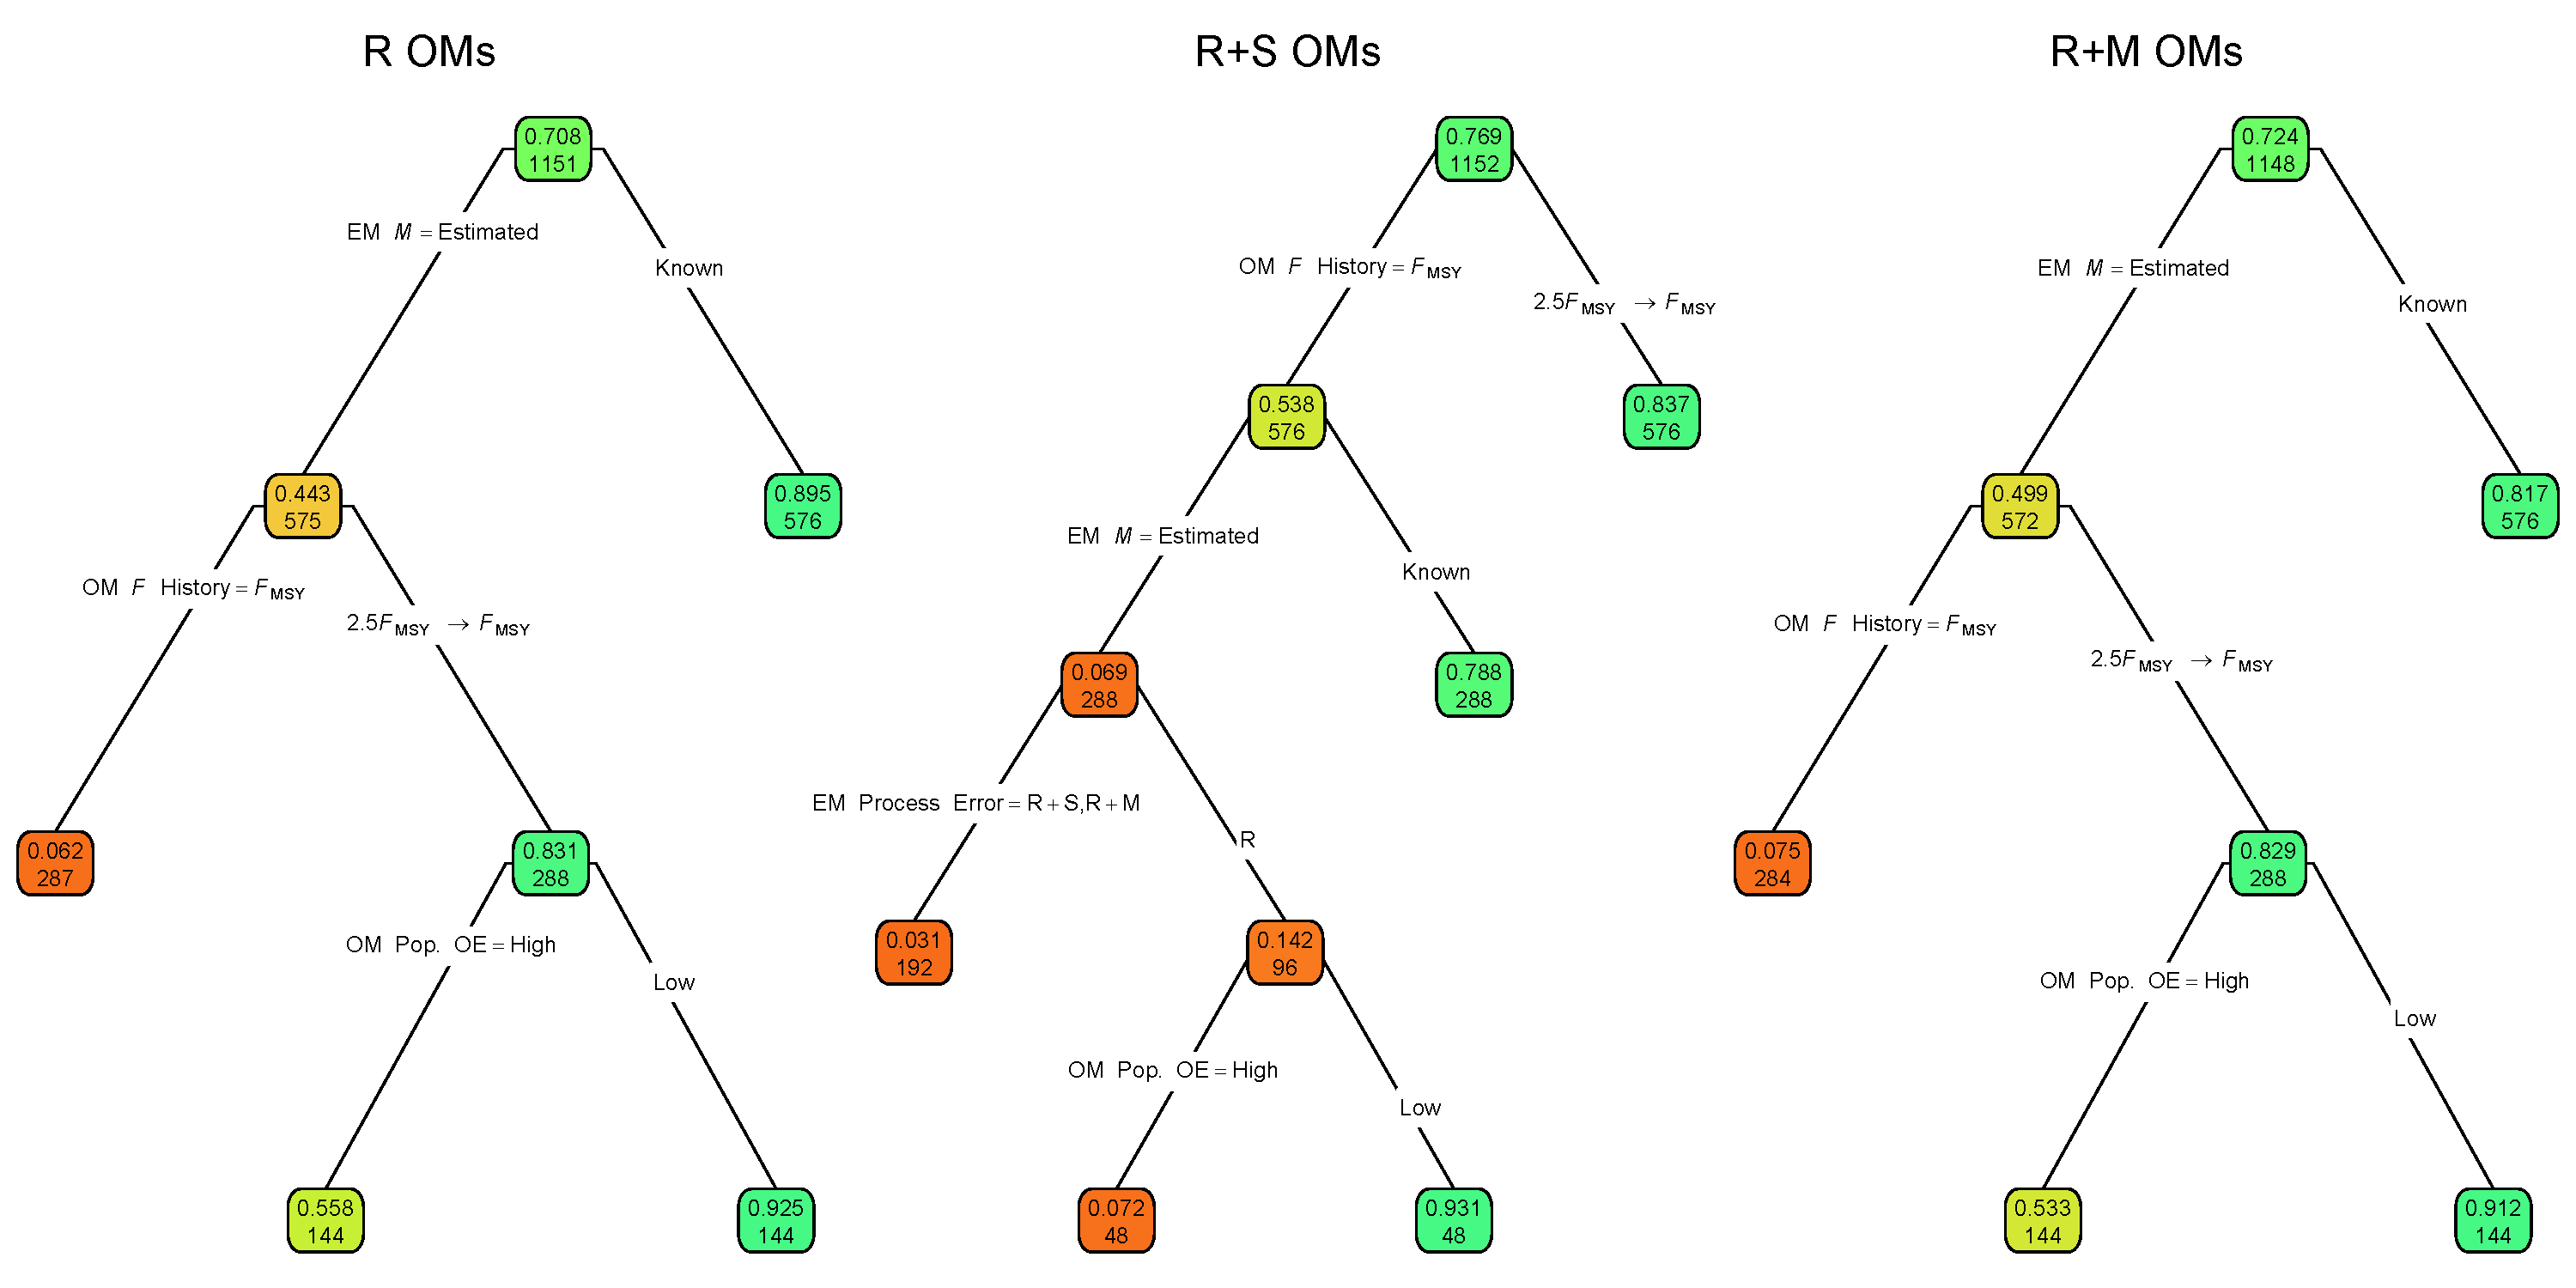
\includegraphics[width = 1.4\textwidth]{term_ssb_corr_regtree_plots}
\end{center}
\caption{\DIFaddFL{Regression trees indicating primary factors determining reductions in sums of squares for the correlation of terminal year SSB estimates and true values in EMs fitted to operating models (OMs) with process error on recruitment only (R), recruitment and apparent survival (R+S), or recruitment and natural mortality (R+M). Each node shows the median error (top) and number of observations (bottom) for the corresponding subset. Lower or higher median correlations are indicated by more red or green polygons, respectively.}}\label{term_ssb_corr_regtree}
\end{figure}
\end{landscape}
\pagebreak

\begin{table}
\caption{\DIFaddFL{Operating (OM) and estimating model (EM) attributes used in analyses of deviance reduction and classification and regression trees. R, R+S, and R+M, denote models (OM or EM) with process error on recruitment only, recruitment and apparent survival, and recruitment and natural mortality, respectively. SD denotes standard deviation and }\Fmsy \DIFaddFL{is the fishing mortality rate that acheives maximum sustainable yield.}}\label{factor_table}
{\begin{center}
\begin{tabular}{lc}
\hline\hline
\multicolumn{1}{c}{\DIFaddFL{Factor}}&\multicolumn{1}{c}{\DIFaddFL{Levels}}\tabularnewline
\hline
\DIFaddFL{OM Process error}&\DIFaddFL{R, R+S, R+M}\tabularnewline
\DIFaddFL{OM Fishing History}&\DIFaddFL{$F_{\text{MSY}}$, $2.5F_{\text{MSY}} \rightarrow F_{\text{MSY}}$}\tabularnewline
\DIFaddFL{OM Covariate effect size ($\beta_E$)}&\DIFaddFL{0, 0.25, 0.5}\tabularnewline
\DIFaddFL{OM Population Observation Error}&\DIFaddFL{Low, High}\tabularnewline
\DIFaddFL{OM Covariate Observation Error}&\DIFaddFL{Low ($\sigma_e = 0.1$), High ($\sigma_e = 0.5$)}\tabularnewline
\DIFaddFL{OM Covariate Process Error SD ($\sigma_E$)}&\DIFaddFL{0.1, 0.5}\tabularnewline
\DIFaddFL{OM Covariate Process Error Correlation ($\rho_E$)}&\DIFaddFL{0, 0.5}\tabularnewline
\DIFaddFL{EM Process Error}&\DIFaddFL{R, R+S, R+M}\tabularnewline
\DIFaddFL{EM Covariate Effect}&\DIFaddFL{None ($\beta_E = 0$), $\beta_E$ estimated}\tabularnewline
\DIFaddFL{EM Median Natural Mortality Rate Parameter ($\beta_M$)}&\DIFaddFL{Known, Estimated}\tabularnewline
\hline
\end{tabular}\end{center}
}
\end{table}
\pagebreak
\clearpage

\begin{table}
\caption{\DIFaddFL{For each OM process error source (columns), percent reduction in deviance for linear regression models fit to errors in estimation of the Hessian-based standard error of the estimates of the covariate effect on $M$ ($\widehat {\text{SE}}\left(\widehat \beta_E\right)$) with each OM and EM factor (rows) included individually, combined, and with second and third order interactions.}}\label{bias_ecov_beta_se_PRD_table}
{\begin{center}
\begin{tabular}{lrrr}
\hline\hline
\multicolumn{1}{l}{\DIFaddFL{Factor}}&\multicolumn{1}{c}{\DIFaddFL{R}}&\multicolumn{1}{c}{\DIFaddFL{R+S}}&\multicolumn{1}{c}{\DIFaddFL{R+M}}\tabularnewline
\hline
\DIFaddFL{OM $F$ history}& \DIFaddFL{1.84}& \DIFaddFL{2.68}& \DIFaddFL{4.00}\tabularnewline
\DIFaddFL{OM Obs. Error}& \DIFaddFL{0.06}& \DIFaddFL{2.74}& \DIFaddFL{8.04}\tabularnewline
\DIFaddFL{OM $\sigma_e$}& \DIFaddFL{6.27}& \DIFaddFL{7.28}&\DIFaddFL{12.83}\tabularnewline
\DIFaddFL{OM $\sigma_E$}& \DIFaddFL{0.48}& \DIFaddFL{1.05}& \DIFaddFL{0.46}\tabularnewline
\DIFaddFL{OM $\rho_{E}$}& \DIFaddFL{0.17}& \DIFaddFL{0.01}& \DIFaddFL{0.02}\tabularnewline
\DIFaddFL{OM $\beta_{E}$}& \DIFaddFL{0.37}& \DIFaddFL{0.01}& \DIFaddFL{0.05}\tabularnewline
\DIFaddFL{EM Process Error}& \DIFaddFL{2.90}& \DIFaddFL{3.89}& \DIFaddFL{2.98}\tabularnewline
\DIFaddFL{EM $M$ assumption}& \DIFaddFL{0.15}& \DIFaddFL{0.34}& \DIFaddFL{0.47}\tabularnewline
\DIFaddFL{All factors}&\DIFaddFL{13.01}&\DIFaddFL{20.95}&\DIFaddFL{29.24}\tabularnewline
\DIFaddFL{+ All Two Way}&\DIFaddFL{28.58}&\DIFaddFL{32.25}&\DIFaddFL{42.77}\tabularnewline
\DIFaddFL{+ All Three Way}&\DIFaddFL{44.44}&\DIFaddFL{42.83}&\DIFaddFL{51.84}\tabularnewline
\hline
\end{tabular}\end{center}
}
\end{table}
\pagebreak

\begin{table}
\caption{\DIFaddFL{For each OM process error source (columns), percent reduction in deviance for linear regression models fit to errors in estimation of the Hessian-based standard error of the estimates of the median $M$ parameter ($\widehat {\text{SE}}\left(\widehat \beta_M\right)$) with each OM and EM factor (rows) included individually, combined, and with second and third order interactions.}}\label{median_M_se_bias_PRD_table}
{\begin{center}
\begin{tabular}{lrrr}
\hline\hline
\multicolumn{1}{l}{\DIFaddFL{Factor}}&\multicolumn{1}{c}{\DIFaddFL{R}}&\multicolumn{1}{c}{\DIFaddFL{R+S}}&\multicolumn{1}{c}{\DIFaddFL{R+M}}\tabularnewline
\hline
\DIFaddFL{OM $F$ history}& \DIFaddFL{0.55}&\DIFaddFL{12.91}& \DIFaddFL{3.65}\tabularnewline
\DIFaddFL{OM Obs. Error}& \DIFaddFL{0.98}& \DIFaddFL{0.01}& \DIFaddFL{0.07}\tabularnewline
\DIFaddFL{OM $\sigma_e$}&\DIFaddFL{\textless  0.01}& \DIFaddFL{0.03}& \DIFaddFL{0.11}\tabularnewline
\DIFaddFL{OM $\sigma_E$}& \DIFaddFL{0.13}& \DIFaddFL{0.03}& \DIFaddFL{0.19}\tabularnewline
\DIFaddFL{OM $\rho_{E}$}&\DIFaddFL{\textless  0.01}& \DIFaddFL{0.02}&\DIFaddFL{\textless  0.01}\tabularnewline
\DIFaddFL{OM $\beta_{E}$}& \DIFaddFL{0.12}& \DIFaddFL{0.07}& \DIFaddFL{0.23}\tabularnewline
\DIFaddFL{EM Process Error}& \DIFaddFL{3.16}& \DIFaddFL{8.79}& \DIFaddFL{6.83}\tabularnewline
\DIFaddFL{EM $\beta_{E}$ assumption}& \DIFaddFL{0.18}& \DIFaddFL{8.96}& \DIFaddFL{3.81}\tabularnewline
\DIFaddFL{All factors}& \DIFaddFL{5.32}&\DIFaddFL{28.39}&\DIFaddFL{14.71}\tabularnewline
\DIFaddFL{+ All Two Way}&\DIFaddFL{11.80}&\DIFaddFL{44.67}&\DIFaddFL{22.70}\tabularnewline
\DIFaddFL{+ All Three Way}&\DIFaddFL{17.83}&\DIFaddFL{51.54}&\DIFaddFL{29.46}\tabularnewline
\hline
\end{tabular}\end{center}
}
\end{table}
\pagebreak

\begin{table}
\caption{\DIFaddFL{For each OM process error source (columns), percent reduction in deviance for linear regression models fit to log-transformed RMSE of terminal year $M$ with each OM and EM factor (rows) included individually, combined, and with second and third order interactions.}}\label{rmse_M_PRD_table}
{\begin{center}
\begin{tabular}{lrrr}
\hline\hline
\multicolumn{1}{l}{\DIFaddFL{Factor}}&\multicolumn{1}{c}{\DIFaddFL{R}}&\multicolumn{1}{c}{\DIFaddFL{R+S}}&\multicolumn{1}{c}{\DIFaddFL{R+M}}\tabularnewline
\hline
\DIFaddFL{OM $F$ history}& \DIFaddFL{0.26}& \DIFaddFL{2.21}&\DIFaddFL{14.65}\tabularnewline
\DIFaddFL{OM Obs. Error}& \DIFaddFL{1.65}& \DIFaddFL{0.71}& \DIFaddFL{4.68}\tabularnewline
\DIFaddFL{$OM \sigma_e$}& \DIFaddFL{0.02}& \DIFaddFL{0.16}& \DIFaddFL{0.01}\tabularnewline
\DIFaddFL{$OM \sigma_E$}& \DIFaddFL{1.06}& \DIFaddFL{1.23}& \DIFaddFL{0.84}\tabularnewline
\DIFaddFL{$OM \rho_{E}$}& \DIFaddFL{0.02}& \DIFaddFL{0.01}&\DIFaddFL{\textless  0.01}\tabularnewline
\DIFaddFL{OM $\beta_{E}$}& \DIFaddFL{3.73}& \DIFaddFL{1.94}& \DIFaddFL{1.14}\tabularnewline
\DIFaddFL{EM Process Error}& \DIFaddFL{2.04}& \DIFaddFL{3.85}& \DIFaddFL{0.87}\tabularnewline
\DIFaddFL{$EM \beta_{E}$ assumption}& \DIFaddFL{0.19}& \DIFaddFL{0.59}& \DIFaddFL{0.07}\tabularnewline
\DIFaddFL{EM $M$ assumption}&\DIFaddFL{22.28}&\DIFaddFL{45.15}&\DIFaddFL{44.70}\tabularnewline
\DIFaddFL{All factors}&\DIFaddFL{32.83}&\DIFaddFL{56.71}&\DIFaddFL{66.99}\tabularnewline
\DIFaddFL{+ All Two Way}&\DIFaddFL{57.65}&\DIFaddFL{84.17}&\DIFaddFL{87.96}\tabularnewline
\DIFaddFL{+ All Three Way}&\DIFaddFL{74.93}&\DIFaddFL{94.57}&\DIFaddFL{91.94}\tabularnewline
\hline
\end{tabular}\end{center}
}
\end{table}
\pagebreak

\begin{table}
\caption{\DIFaddFL{For each OM process error source (columns), percent reduction in deviance for linear regression models fit to correlation of terminal year $M$ estimates and true values with each OM and EM factor (rows) included individually, combined, and with second and third order interactions.}}\label{corr_M_PRD_table}
{\begin{center}
\begin{tabular}{lrrr}
\hline\hline
\multicolumn{1}{l}{\DIFaddFL{Factor}}&\multicolumn{1}{c}{\DIFaddFL{R}}&\multicolumn{1}{c}{\DIFaddFL{R+S}}&\multicolumn{1}{c}{\DIFaddFL{R+M}}\tabularnewline
\hline
\DIFaddFL{OM $F$ history}& \DIFaddFL{0.05}& \DIFaddFL{0.02}& \DIFaddFL{0.37}\tabularnewline
\DIFaddFL{OM Obs. Error}& \DIFaddFL{2.00}& \DIFaddFL{0.89}& \DIFaddFL{3.73}\tabularnewline
\DIFaddFL{$OM \sigma_e$}& \DIFaddFL{2.30}& \DIFaddFL{2.56}& \DIFaddFL{0.37}\tabularnewline
\DIFaddFL{$OM \sigma_E$}&\DIFaddFL{14.91}&\DIFaddFL{13.78}& \DIFaddFL{3.03}\tabularnewline
\DIFaddFL{$OM \rho_{E}$}& \DIFaddFL{1.98}& \DIFaddFL{0.33}& \DIFaddFL{0.14}\tabularnewline
\DIFaddFL{OM $\beta_{E}$}& \DIFaddFL{0.41}& \DIFaddFL{3.76}& \DIFaddFL{3.87}\tabularnewline
\DIFaddFL{EM Process Error}& \DIFaddFL{0.43}& \DIFaddFL{1.52}& \DIFaddFL{0.62}\tabularnewline
\DIFaddFL{$EM \beta_{E}$ assumption}&\DIFaddFL{12.72}&\DIFaddFL{12.30}& \DIFaddFL{1.56}\tabularnewline
\DIFaddFL{EM $M$ assumption}&\DIFaddFL{12.34}& \DIFaddFL{7.16}& \DIFaddFL{3.03}\tabularnewline
\DIFaddFL{All factors}&\DIFaddFL{42.11}&\DIFaddFL{38.31}&\DIFaddFL{15.76}\tabularnewline
\DIFaddFL{+ All Two Way}&\DIFaddFL{63.38}&\DIFaddFL{62.40}&\DIFaddFL{31.99}\tabularnewline
\DIFaddFL{+ All Three Way}&\DIFaddFL{72.79}&\DIFaddFL{75.98}&\DIFaddFL{46.62}\tabularnewline
\hline
\end{tabular}\end{center}
}
\end{table}
\pagebreak

\begin{table}
\caption{\DIFaddFL{For each OM process error source (columns), percent reduction in deviance for linear regression models fit to log-transformed RMSE of terminal year SSB with each OM and EM factor (rows) included individually, combined, and with second and third order interactions.}}\label{rmse_SSB_PRD_table}
{\begin{center}
\begin{tabular}{lrrr}
\hline\hline
\multicolumn{1}{l}{\DIFaddFL{Factor}}&\multicolumn{1}{c}{\DIFaddFL{R}}&\multicolumn{1}{c}{\DIFaddFL{R+S}}&\multicolumn{1}{c}{\DIFaddFL{R+M}}\tabularnewline
\hline
\DIFaddFL{OM $F$ history}&\DIFaddFL{19.88}&\DIFaddFL{32.67}&\DIFaddFL{20.92}\tabularnewline
\DIFaddFL{OM Obs. Error}& \DIFaddFL{2.21}& \DIFaddFL{0.11}& \DIFaddFL{1.48}\tabularnewline
\DIFaddFL{$OM \sigma_e$}& \DIFaddFL{0.05}& \DIFaddFL{0.16}& \DIFaddFL{0.03}\tabularnewline
\DIFaddFL{$OM \sigma_E$}& \DIFaddFL{0.08}& \DIFaddFL{0.16}& \DIFaddFL{0.02}\tabularnewline
\DIFaddFL{$OM \rho_{E}$}& \DIFaddFL{0.03}&\DIFaddFL{\textless  0.01}& \DIFaddFL{0.02}\tabularnewline
\DIFaddFL{OM $\beta_{E}$}& \DIFaddFL{0.05}& \DIFaddFL{0.03}& \DIFaddFL{0.14}\tabularnewline
\DIFaddFL{EM Process Error}& \DIFaddFL{5.72}& \DIFaddFL{0.13}& \DIFaddFL{5.73}\tabularnewline
\DIFaddFL{$EM \beta_{E}$ assumption}& \DIFaddFL{0.03}& \DIFaddFL{0.79}& \DIFaddFL{0.05}\tabularnewline
\DIFaddFL{EM $M$ assumption}&\DIFaddFL{20.05}&\DIFaddFL{21.11}&\DIFaddFL{19.43}\tabularnewline
\DIFaddFL{All factors}&\DIFaddFL{48.09}&\DIFaddFL{55.17}&\DIFaddFL{47.82}\tabularnewline
\DIFaddFL{+ All Two Way}&\DIFaddFL{79.09}&\DIFaddFL{80.98}&\DIFaddFL{78.40}\tabularnewline
\DIFaddFL{+ All Three Way}&\DIFaddFL{88.30}&\DIFaddFL{89.49}&\DIFaddFL{87.67}\tabularnewline
\hline
\end{tabular}\end{center}
}
\end{table}
\pagebreak

\begin{table}
\caption{\DIFaddFL{For each OM process error source (columns), percent reduction in deviance for linear regression models fit to correlation of terminal year SSB estimates and true values with each OM and EM factor (rows) included individually, combined, and with second and third order interactions.}}\label{corr_ssb_PRD_table}
{\begin{center}
\begin{tabular}{lrrr}
\hline\hline
\multicolumn{1}{l}{\DIFaddFL{Factor}}&\multicolumn{1}{c}{\DIFaddFL{R}}&\multicolumn{1}{c}{\DIFaddFL{R+S}}&\multicolumn{1}{c}{\DIFaddFL{R+M}}\tabularnewline
\hline
\DIFaddFL{OM $F$ history}&\DIFaddFL{19.27}&\DIFaddFL{25.70}&\DIFaddFL{19.59}\tabularnewline
\DIFaddFL{OM Obs. Error}&\DIFaddFL{12.53}& \DIFaddFL{3.60}& \DIFaddFL{9.46}\tabularnewline
\DIFaddFL{$OM \sigma_e$}& \DIFaddFL{0.08}& \DIFaddFL{0.44}& \DIFaddFL{0.09}\tabularnewline
\DIFaddFL{$OM \sigma_E$}& \DIFaddFL{0.10}& \DIFaddFL{0.44}& \DIFaddFL{0.11}\tabularnewline
\DIFaddFL{$OM \rho_{E}$}&\DIFaddFL{\textless  0.01}&\DIFaddFL{\textless  0.01}& \DIFaddFL{0.09}\tabularnewline
\DIFaddFL{OM $\beta_{E}$}& \DIFaddFL{0.09}& \DIFaddFL{0.05}&\DIFaddFL{\textless  0.01}\tabularnewline
\DIFaddFL{EM Process Error}& \DIFaddFL{0.07}& \DIFaddFL{0.92}& \DIFaddFL{0.71}\tabularnewline
\DIFaddFL{$EM \beta_{E}$ assumption}&\DIFaddFL{\textless  0.01}& \DIFaddFL{1.32}& \DIFaddFL{0.38}\tabularnewline
\DIFaddFL{EM $M$ assumption}&\DIFaddFL{28.94}&\DIFaddFL{19.74}&\DIFaddFL{25.36}\tabularnewline
\DIFaddFL{All factors}&\DIFaddFL{61.19}&\DIFaddFL{52.21}&\DIFaddFL{56.09}\tabularnewline
\DIFaddFL{+ All Two Way}&\DIFaddFL{81.48}&\DIFaddFL{72.16}&\DIFaddFL{74.98}\tabularnewline
\DIFaddFL{+ All Three Way}&\DIFaddFL{85.23}&\DIFaddFL{83.22}&\DIFaddFL{80.48}\tabularnewline
\hline
\end{tabular}\end{center}
}
\end{table}
\pagebreak

\clearpage

\subsection*{\DIFadd{Convergence results}}\label{convergence-results}
\DIFaddend \addcontentsline{toc}{subsection}{Convergence results}

\begin{landscape}
\begin{figure}
\begin{center}
\DIFdelbeginFL %DIFDELCMD < 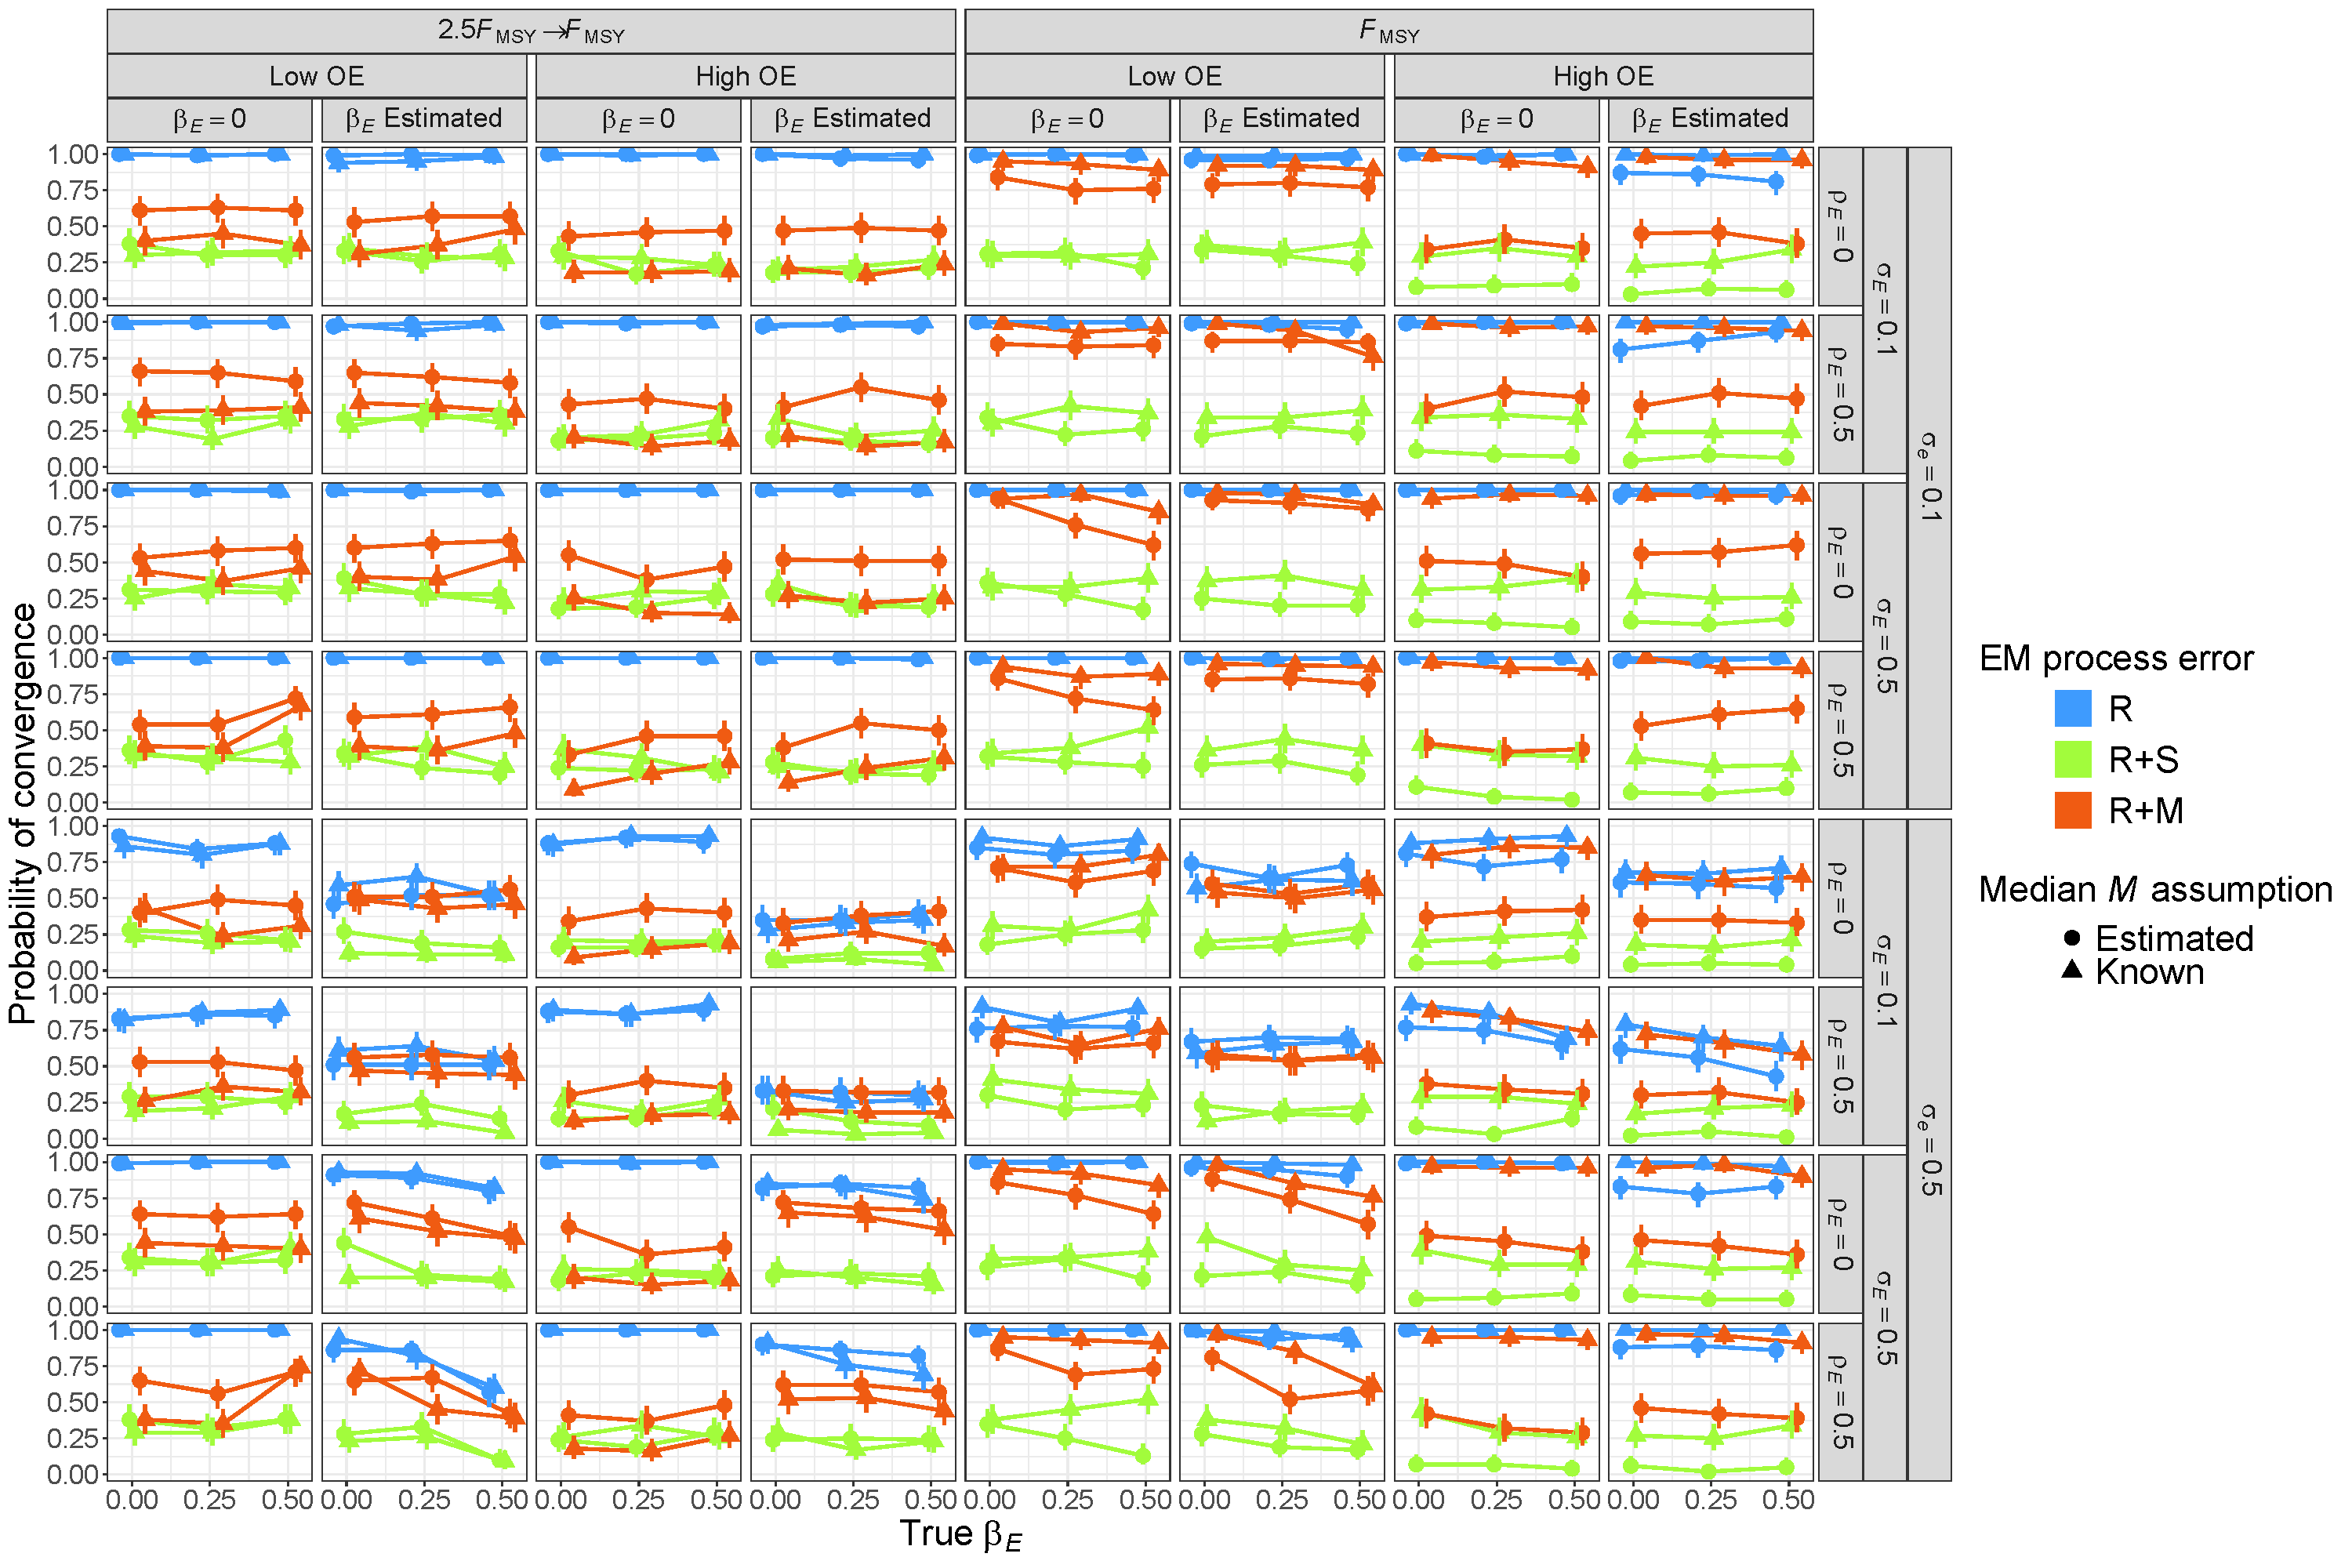
\includegraphics{convergence_Rom}
%DIFDELCMD < %%%
\DIFdelendFL \DIFaddbeginFL 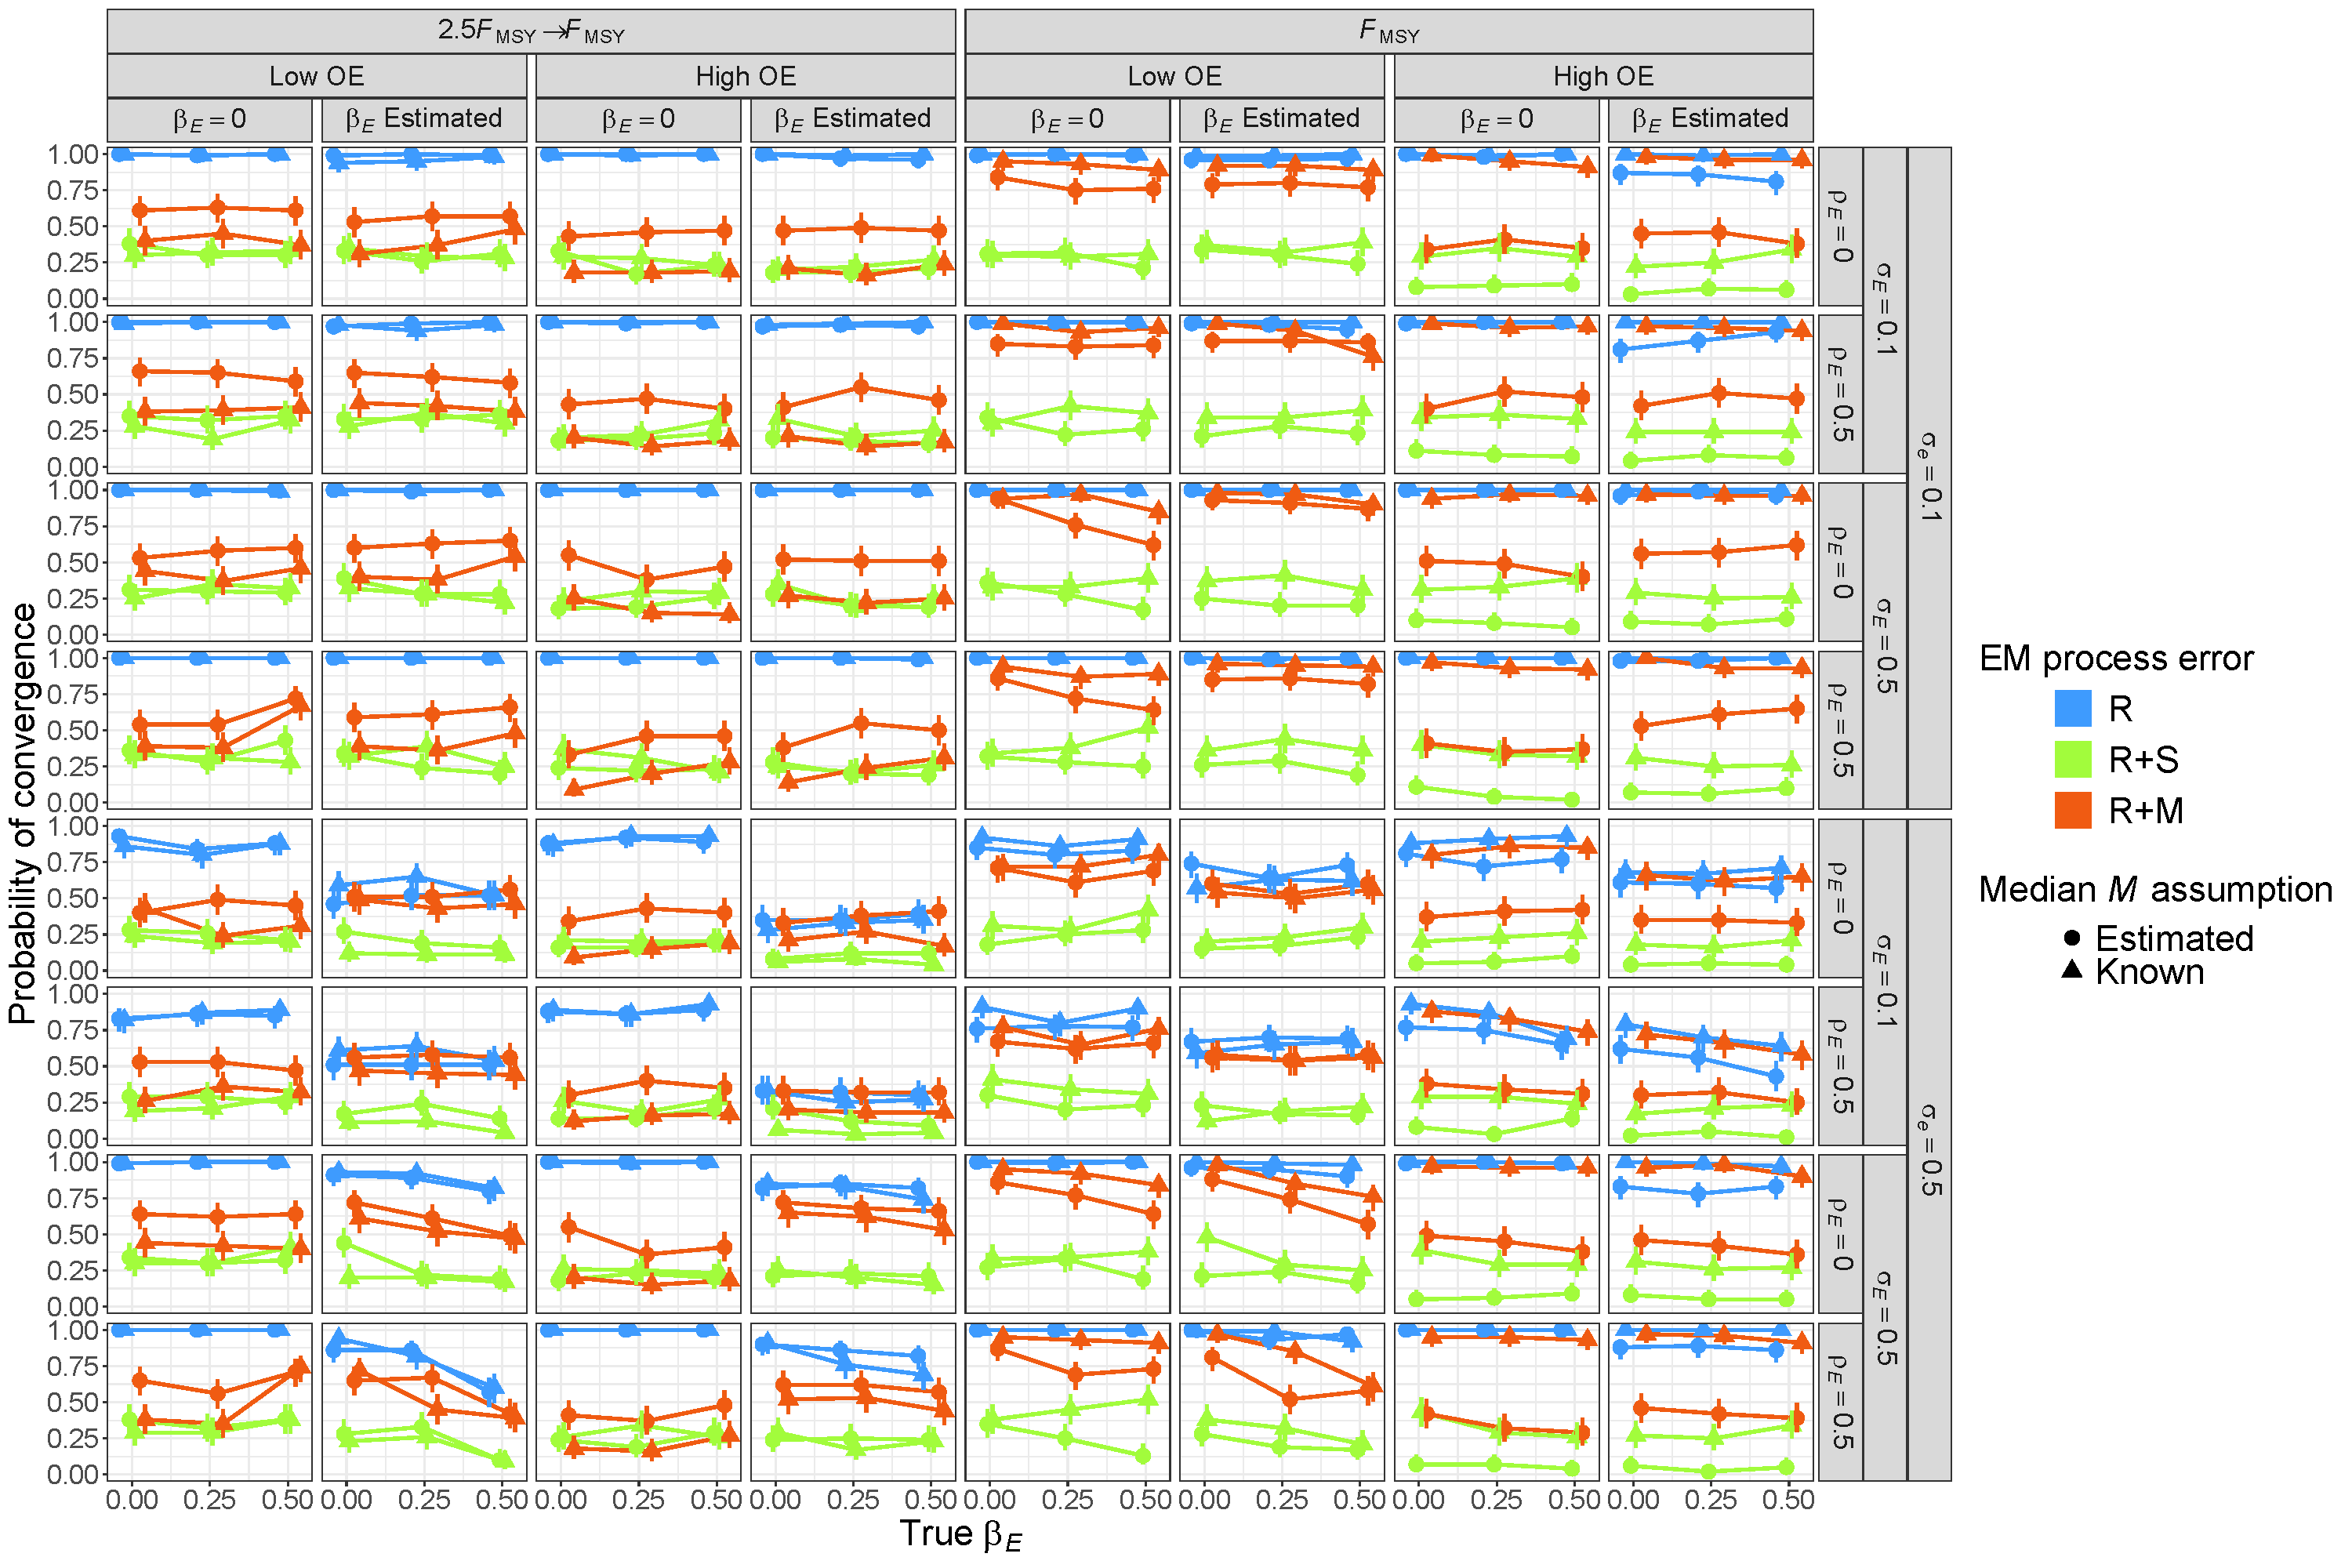
\includegraphics[height = \textheight]{convergence_Rom}
\DIFaddendFL \end{center}
\caption{Estimated probability of fits providing Hessian-based standard errors for EMs assuming alternative process error, that estimate or assume known median \DIFdelbeginFL \DIFdelFL{natural mortality}\DIFdelendFL \DIFaddbeginFL \DIFaddFL{$M$}\DIFaddendFL , and that estimate or assume no covariate effect on median \DIFdelbeginFL \DIFdelFL{natural mortality }\DIFdelendFL \DIFaddbeginFL \DIFaddFL{$M$ }\DIFaddendFL when fitted to R OMs and three levels of true covariate effect on median \DIFdelbeginFL \DIFdelFL{natural mortality }\DIFdelendFL \DIFaddbeginFL \DIFaddFL{$M$ }\DIFaddendFL (x axis). Vertical lines represent 95\% confidence intervals.}\label{convergence_Rom}
\end{figure}
\end{landscape}

\begin{landscape}
\begin{figure}
\begin{center}
\DIFdelbeginFL %DIFDELCMD < 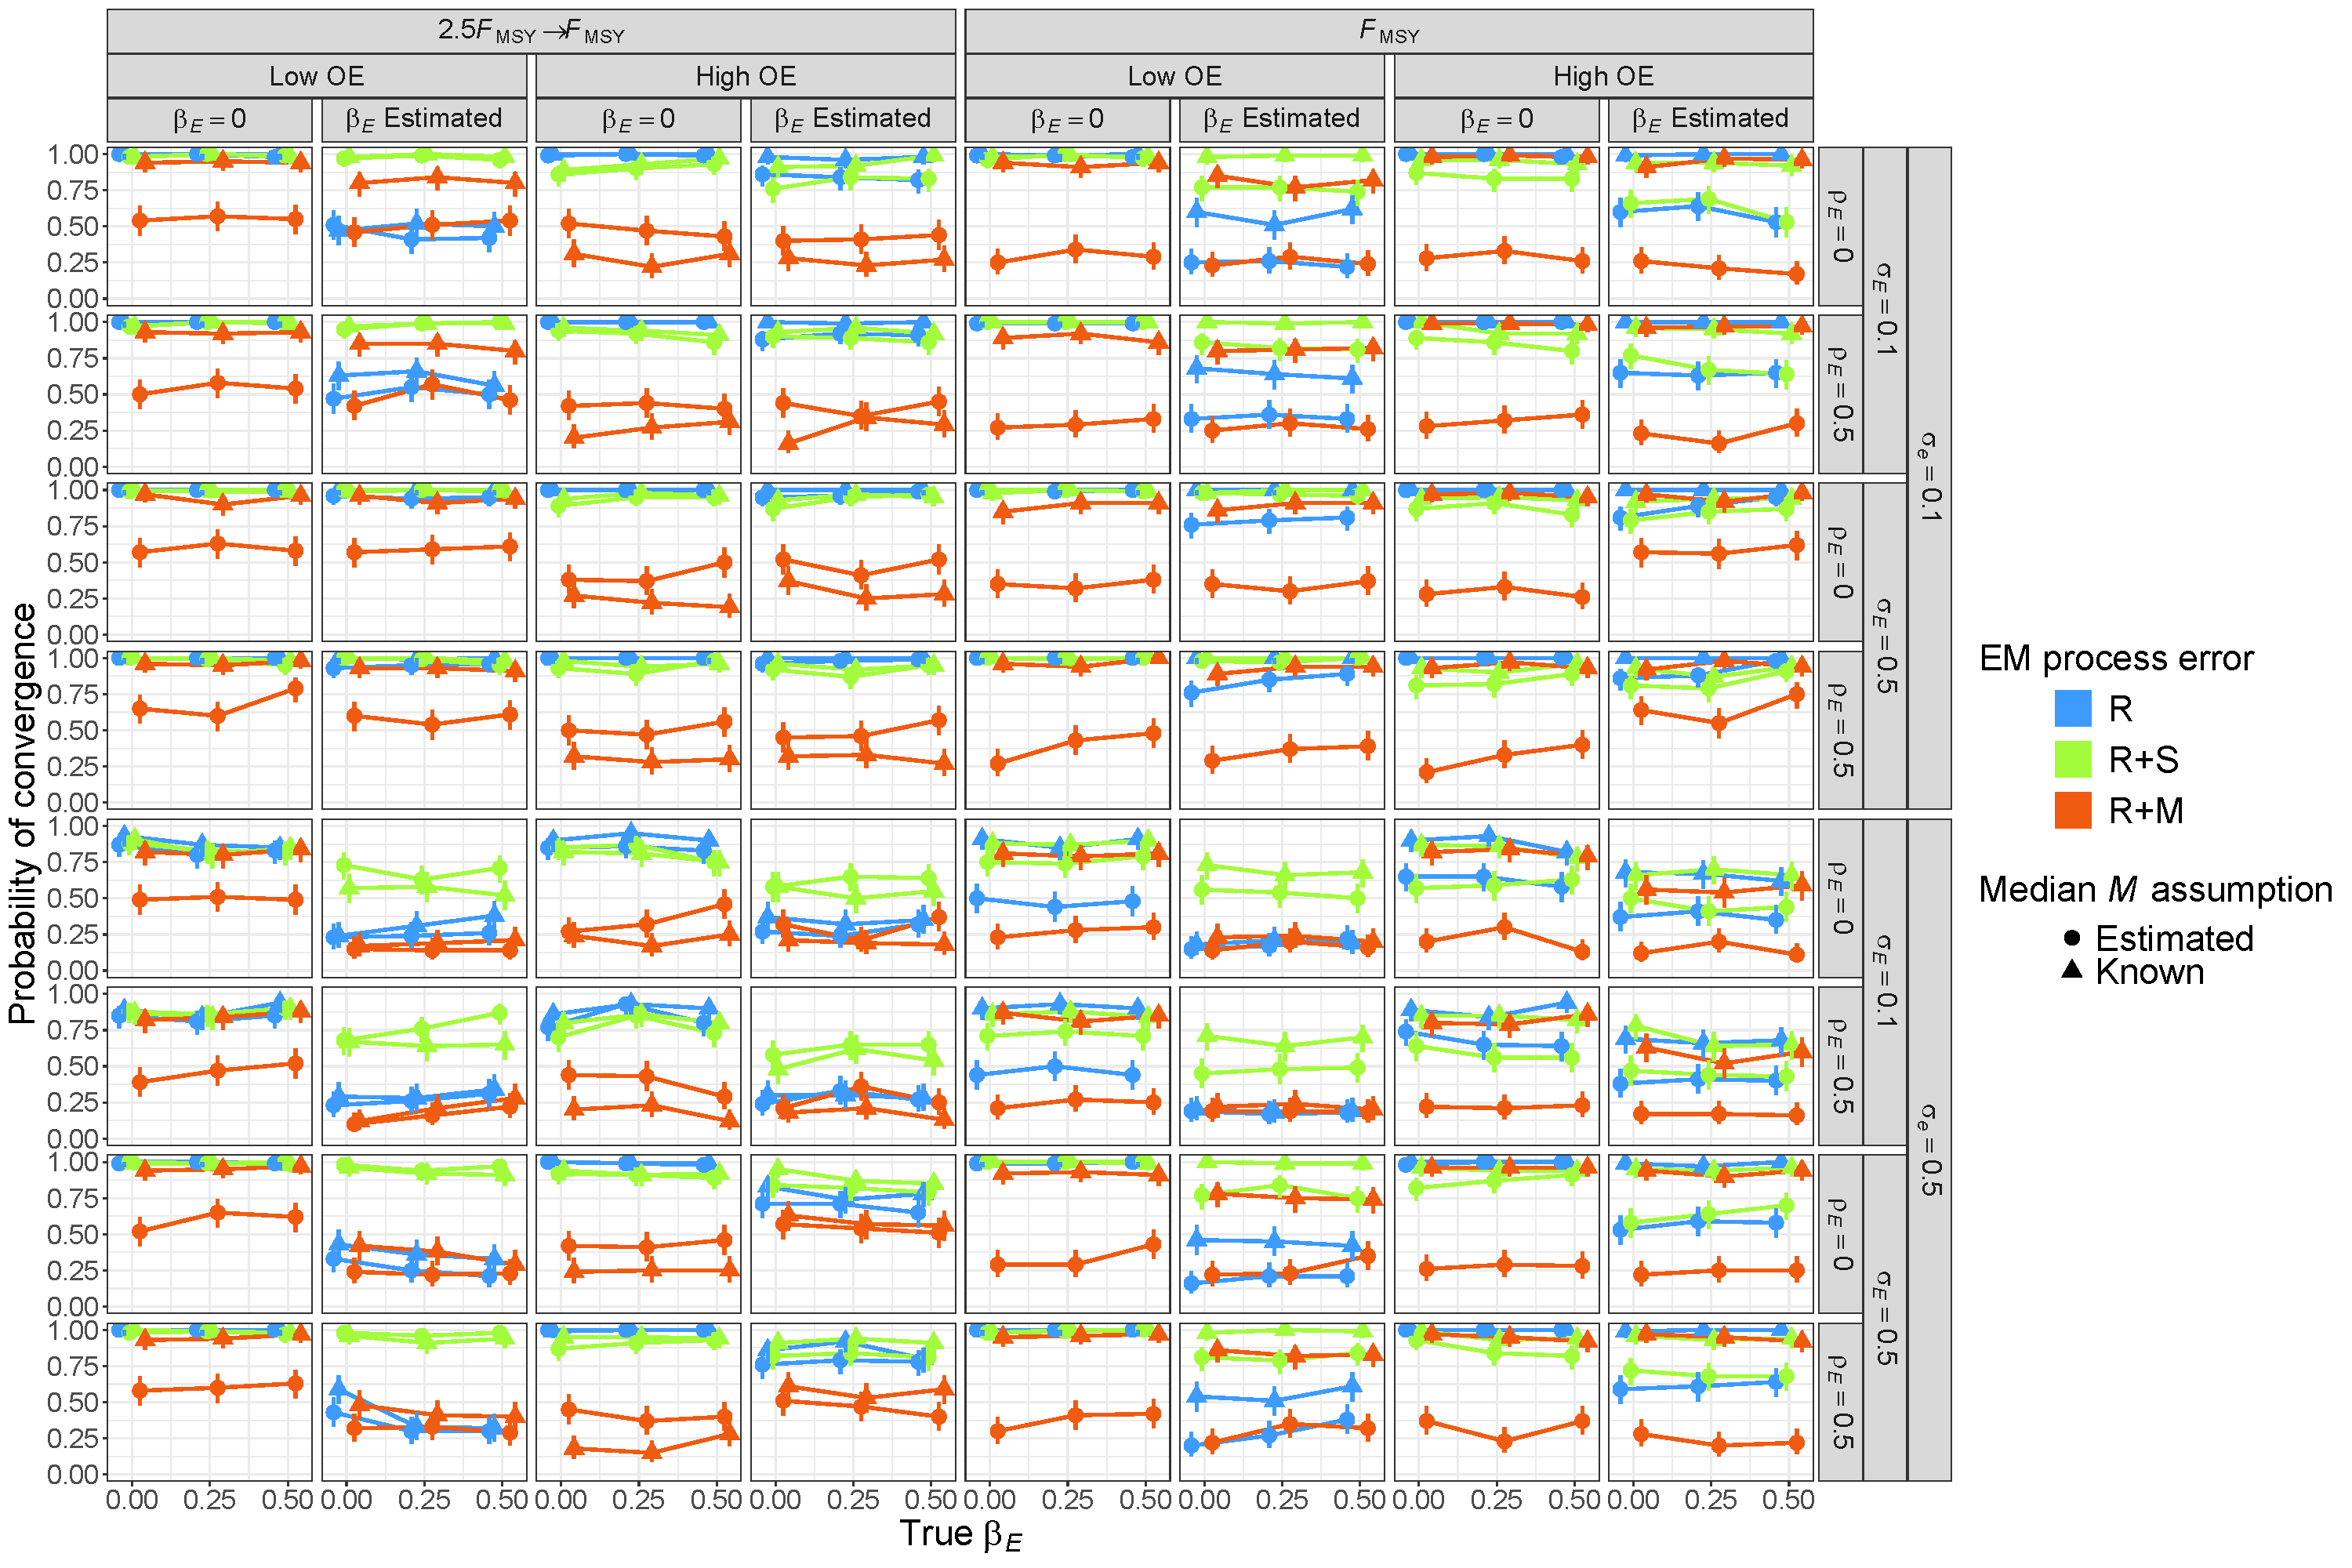
\includegraphics{convergence_RSom}
%DIFDELCMD < %%%
\DIFdelendFL \DIFaddbeginFL 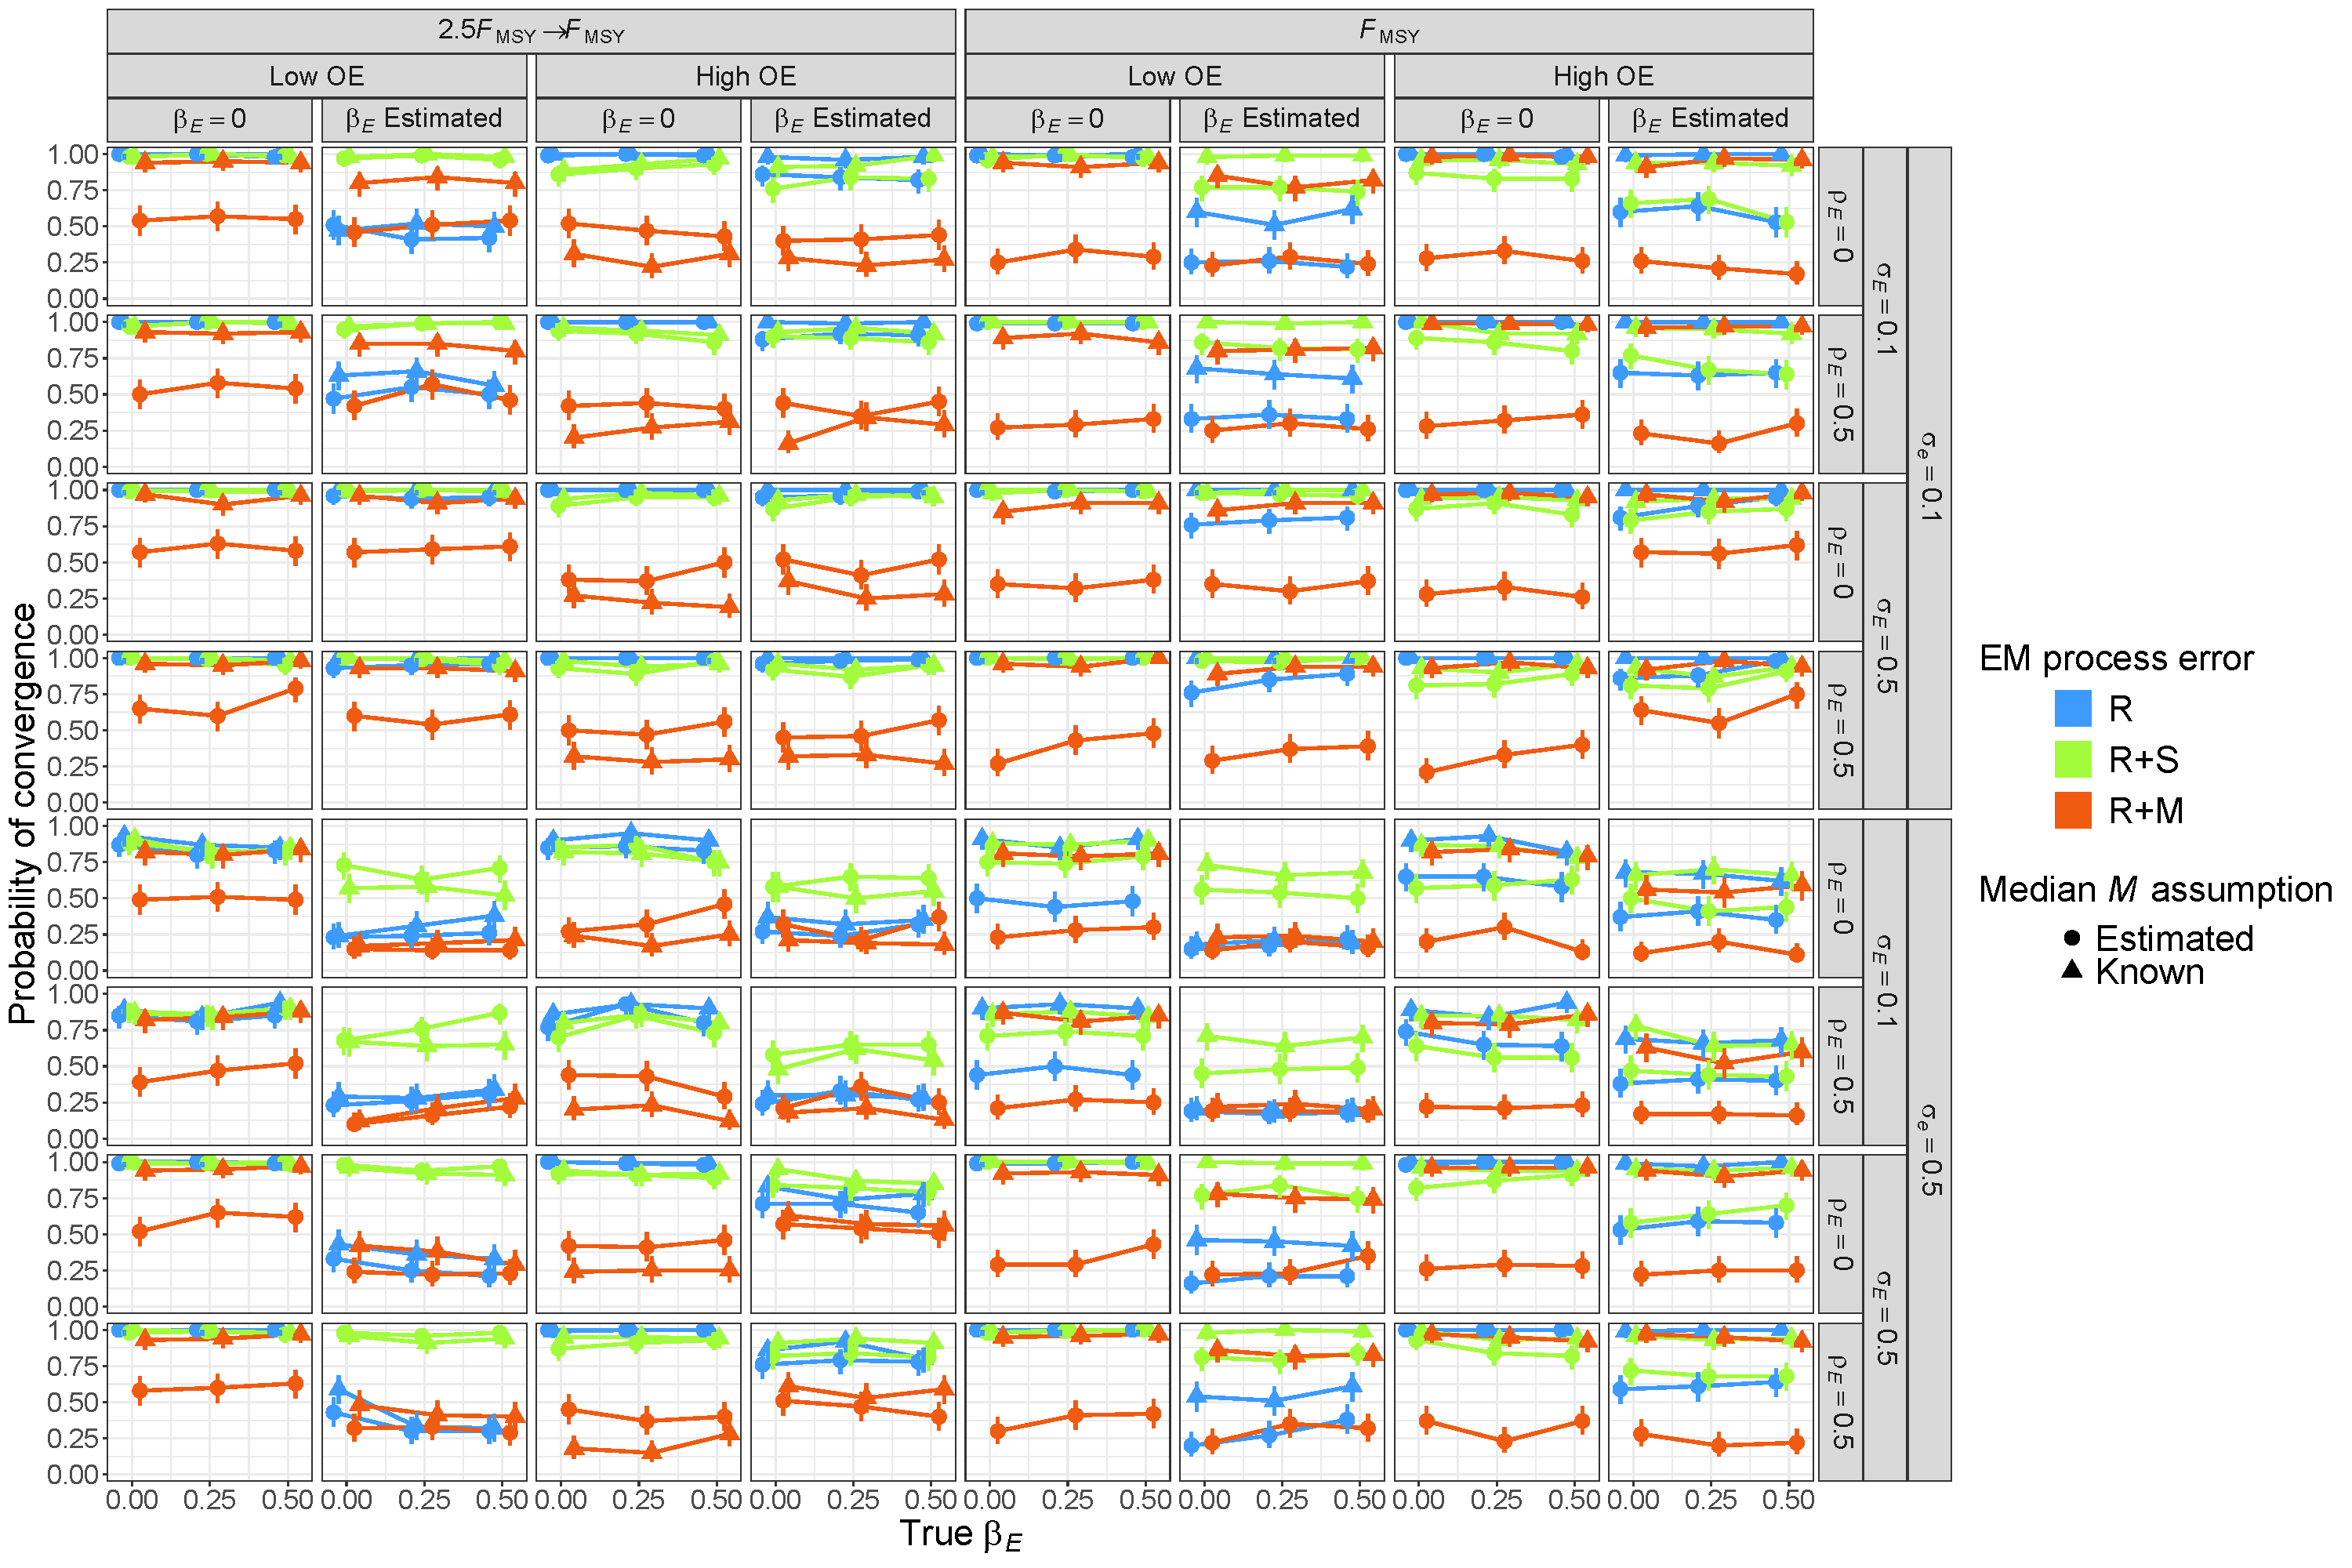
\includegraphics[height = \textheight]{convergence_RSom}
\DIFaddendFL \end{center}
\caption{Estimated probability of fits providing Hessian-based standard errors for EMs assuming alternative process error, that estimate or assume known median \DIFdelbeginFL \DIFdelFL{natural mortality}\DIFdelendFL \DIFaddbeginFL \DIFaddFL{$M$}\DIFaddendFL , and that estimate or assume no covariate effect on median \DIFdelbeginFL \DIFdelFL{natural mortality }\DIFdelendFL \DIFaddbeginFL \DIFaddFL{$M$ }\DIFaddendFL when fitted to R+S OMs and three levels of true covariate effect on median \DIFdelbeginFL \DIFdelFL{natural mortality }\DIFdelendFL \DIFaddbeginFL \DIFaddFL{$M$ }\DIFaddendFL (x axis). Vertical lines represent 95\% confidence intervals.}\label{convergence_RSom}
\end{figure}
\end{landscape}

\begin{landscape}
\begin{figure}
\begin{center}
\DIFdelbeginFL %DIFDELCMD < 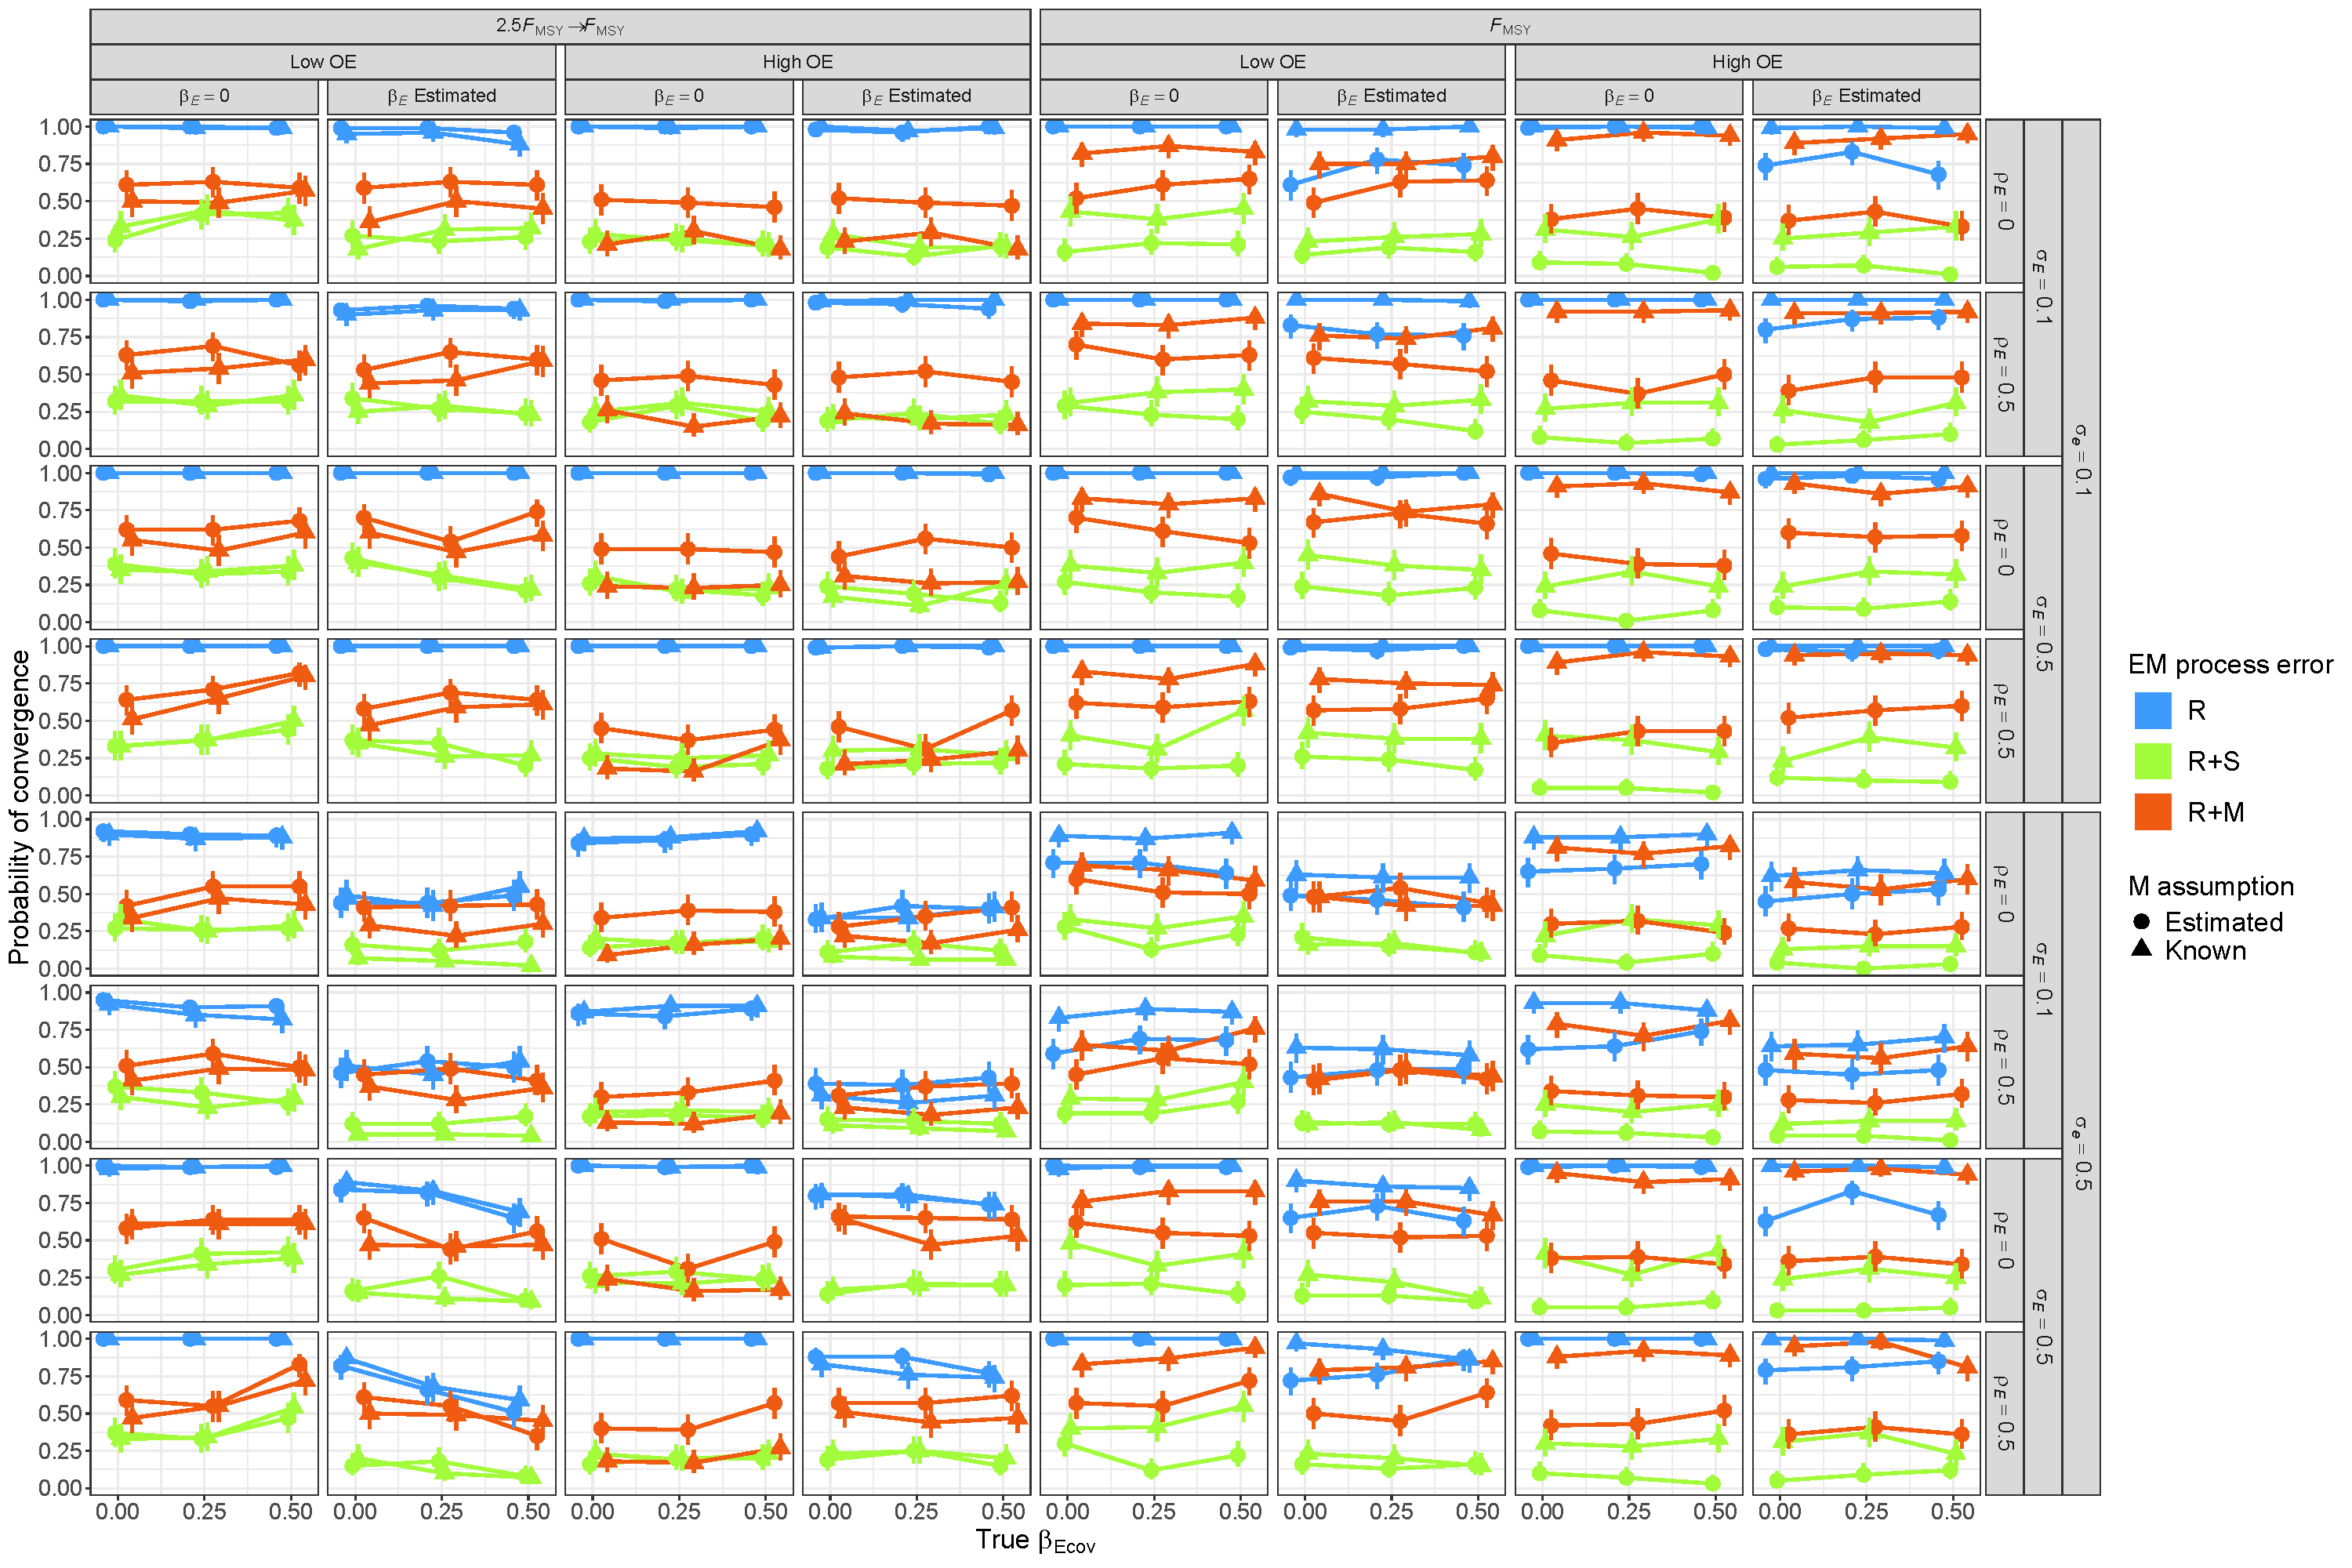
\includegraphics{convergence_RMom}
%DIFDELCMD < %%%
\DIFdelendFL \DIFaddbeginFL 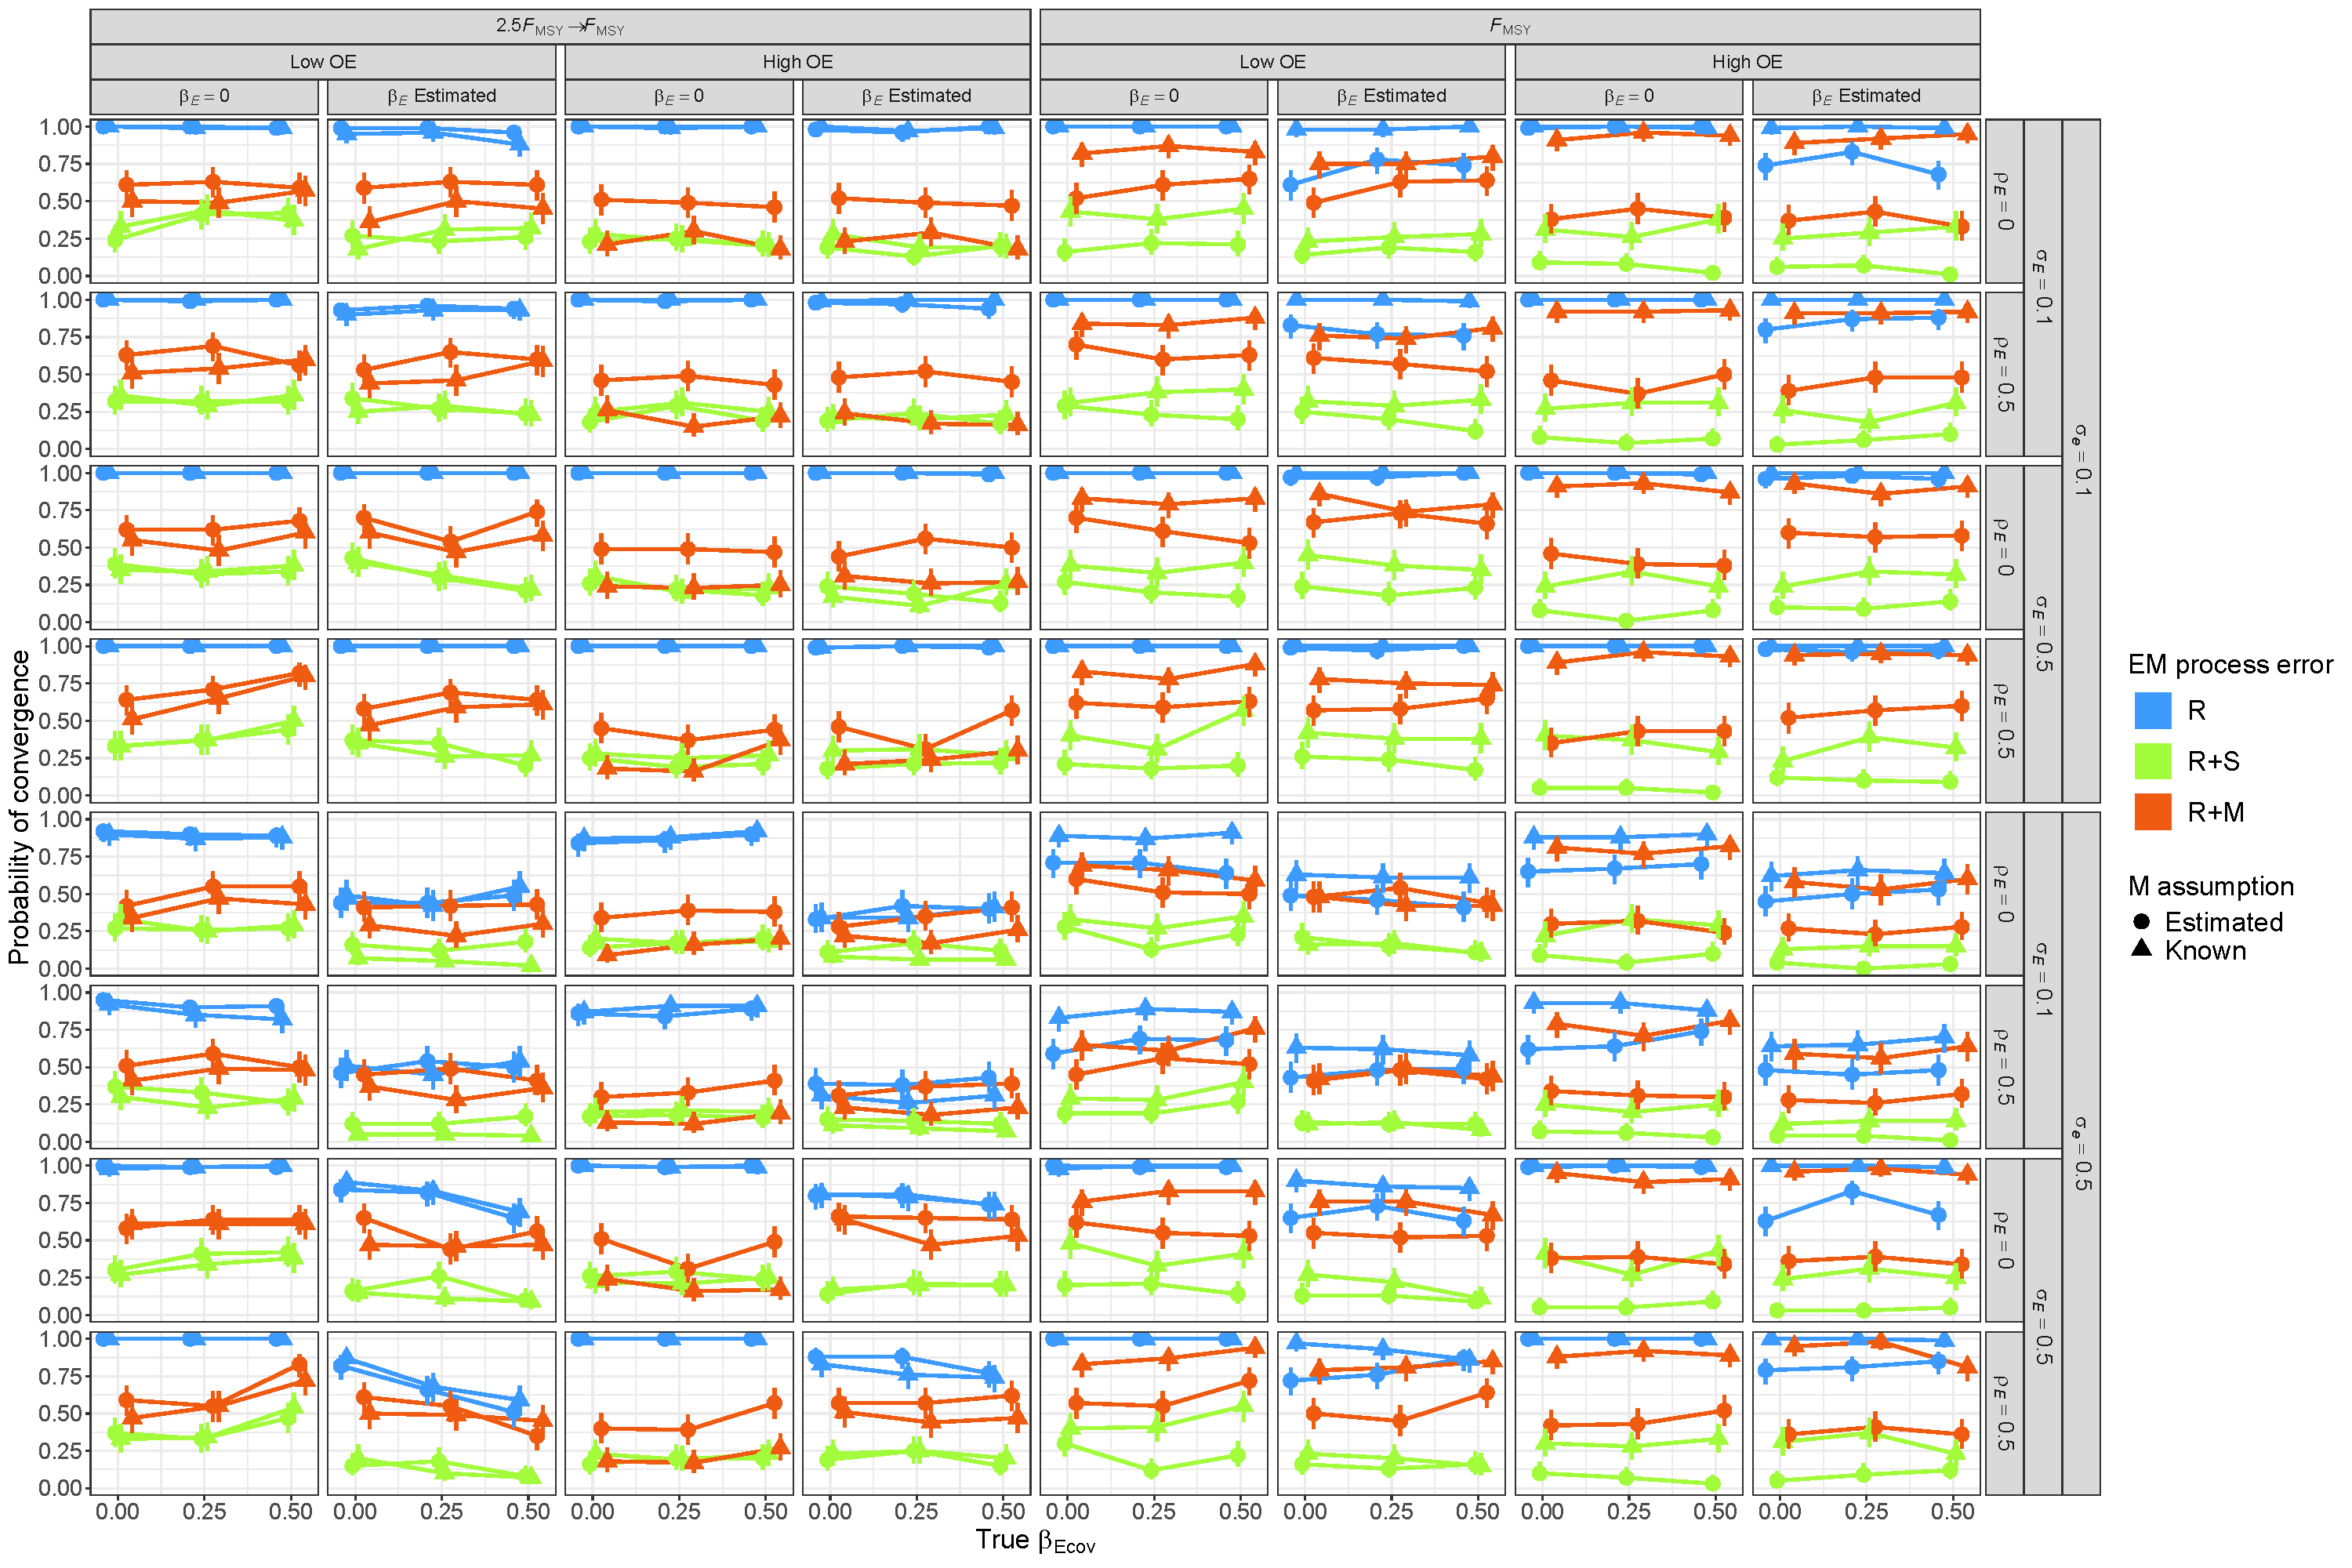
\includegraphics[height = \textheight]{convergence_RMom}
\DIFaddendFL \end{center}
\caption{Estimated probability of fits providing Hessian-based standard errors for EMs assuming alternative process error, that estimate or assume known median \DIFdelbeginFL \DIFdelFL{natural mortality}\DIFdelendFL \DIFaddbeginFL \DIFaddFL{$M$}\DIFaddendFL , and that estimate or assume no covariate effect on median \DIFdelbeginFL \DIFdelFL{natural mortality }\DIFdelendFL \DIFaddbeginFL \DIFaddFL{$M$ }\DIFaddendFL when fitted to R+M OMs and three levels of true covariate effect on median \DIFdelbeginFL \DIFdelFL{natural mortality }\DIFdelendFL \DIFaddbeginFL \DIFaddFL{$M$ }\DIFaddendFL (x axis). Vertical lines represent 95\% confidence intervals.}\label{convergence_RMom}
\end{figure}
\end{landscape}

\DIFdelbegin %DIFDELCMD < \hypertarget{aic-results}{%
%DIFDELCMD < \subsection*{AIC results}\label{aic-results}}
%DIFDELCMD < %%%
\DIFdelend \DIFaddbegin \subsection*{\DIFadd{AIC results}}\label{aic-results}
\DIFaddend \addcontentsline{toc}{subsection}{AIC results}

\begin{landscape}
\begin{figure}
\begin{center}
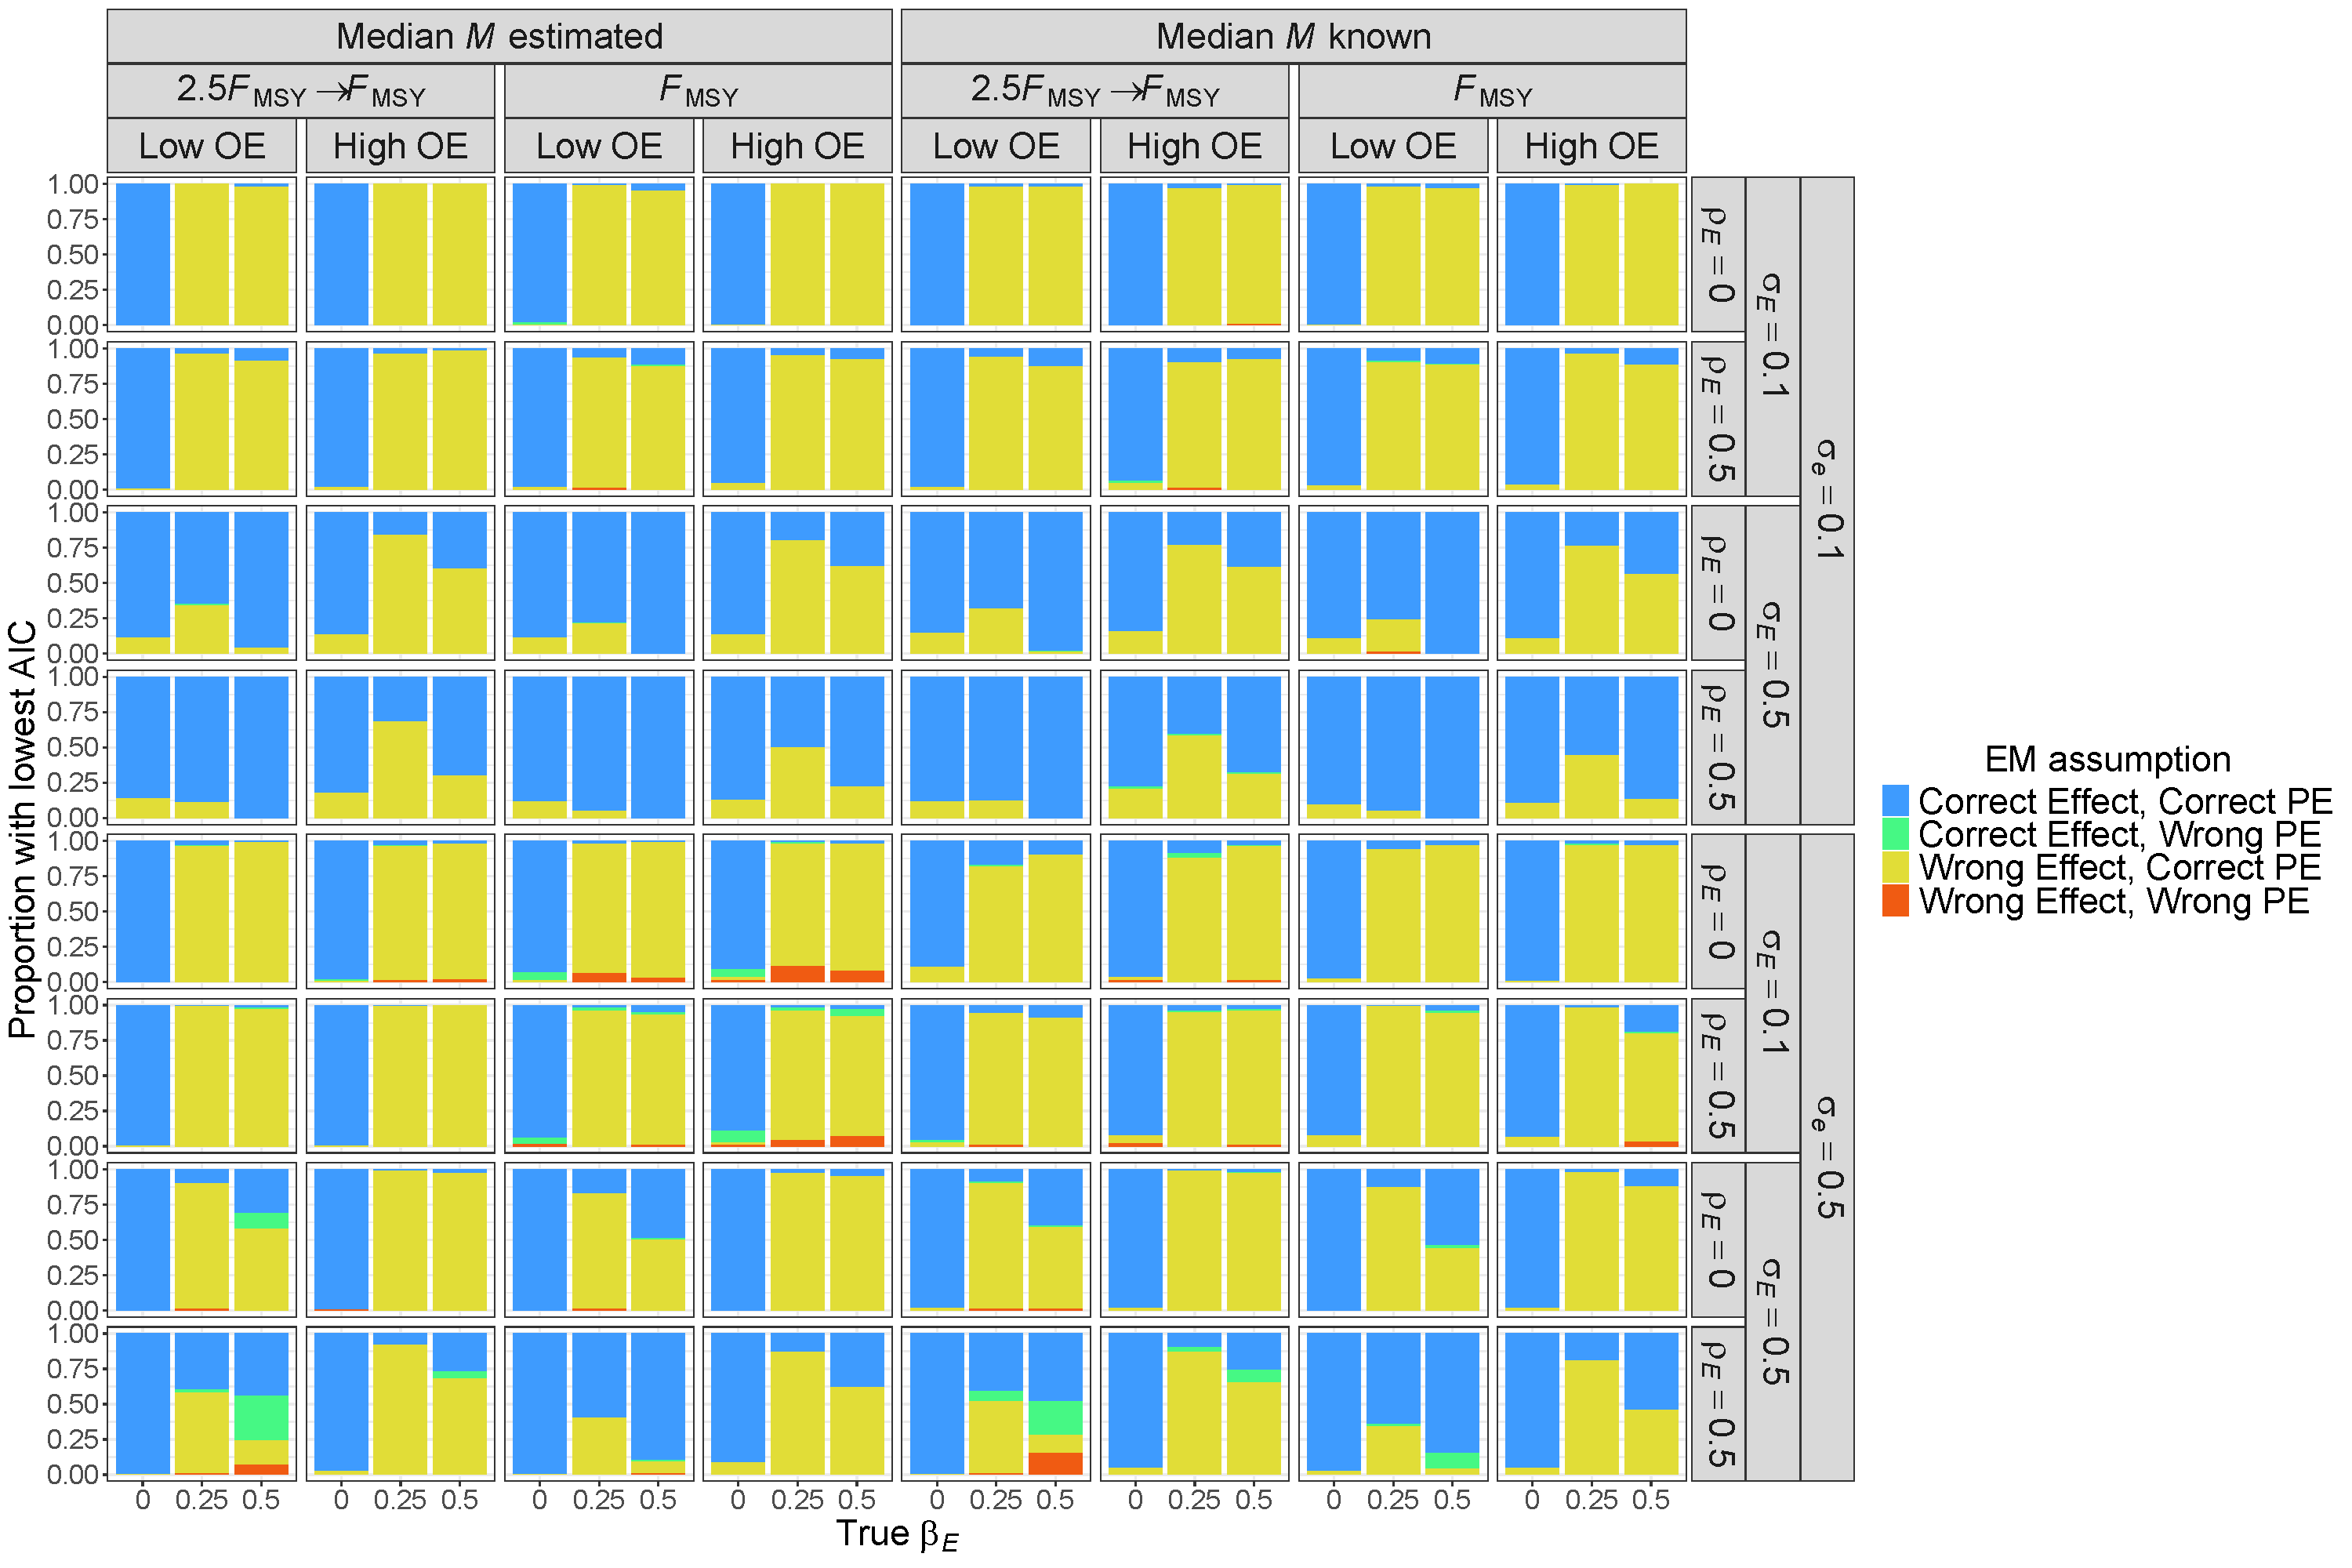
\includegraphics[height = \textheight]{aic_Rom}
\end{center}
\caption{Proportion of simulated data sets for R OMs where the EM type (treatment of environmental covariate and assumed process error type) had the lowest AIC.}\label{aic_Rom}
\end{figure}
\end{landscape}

\begin{landscape}
\begin{figure}
\begin{center}
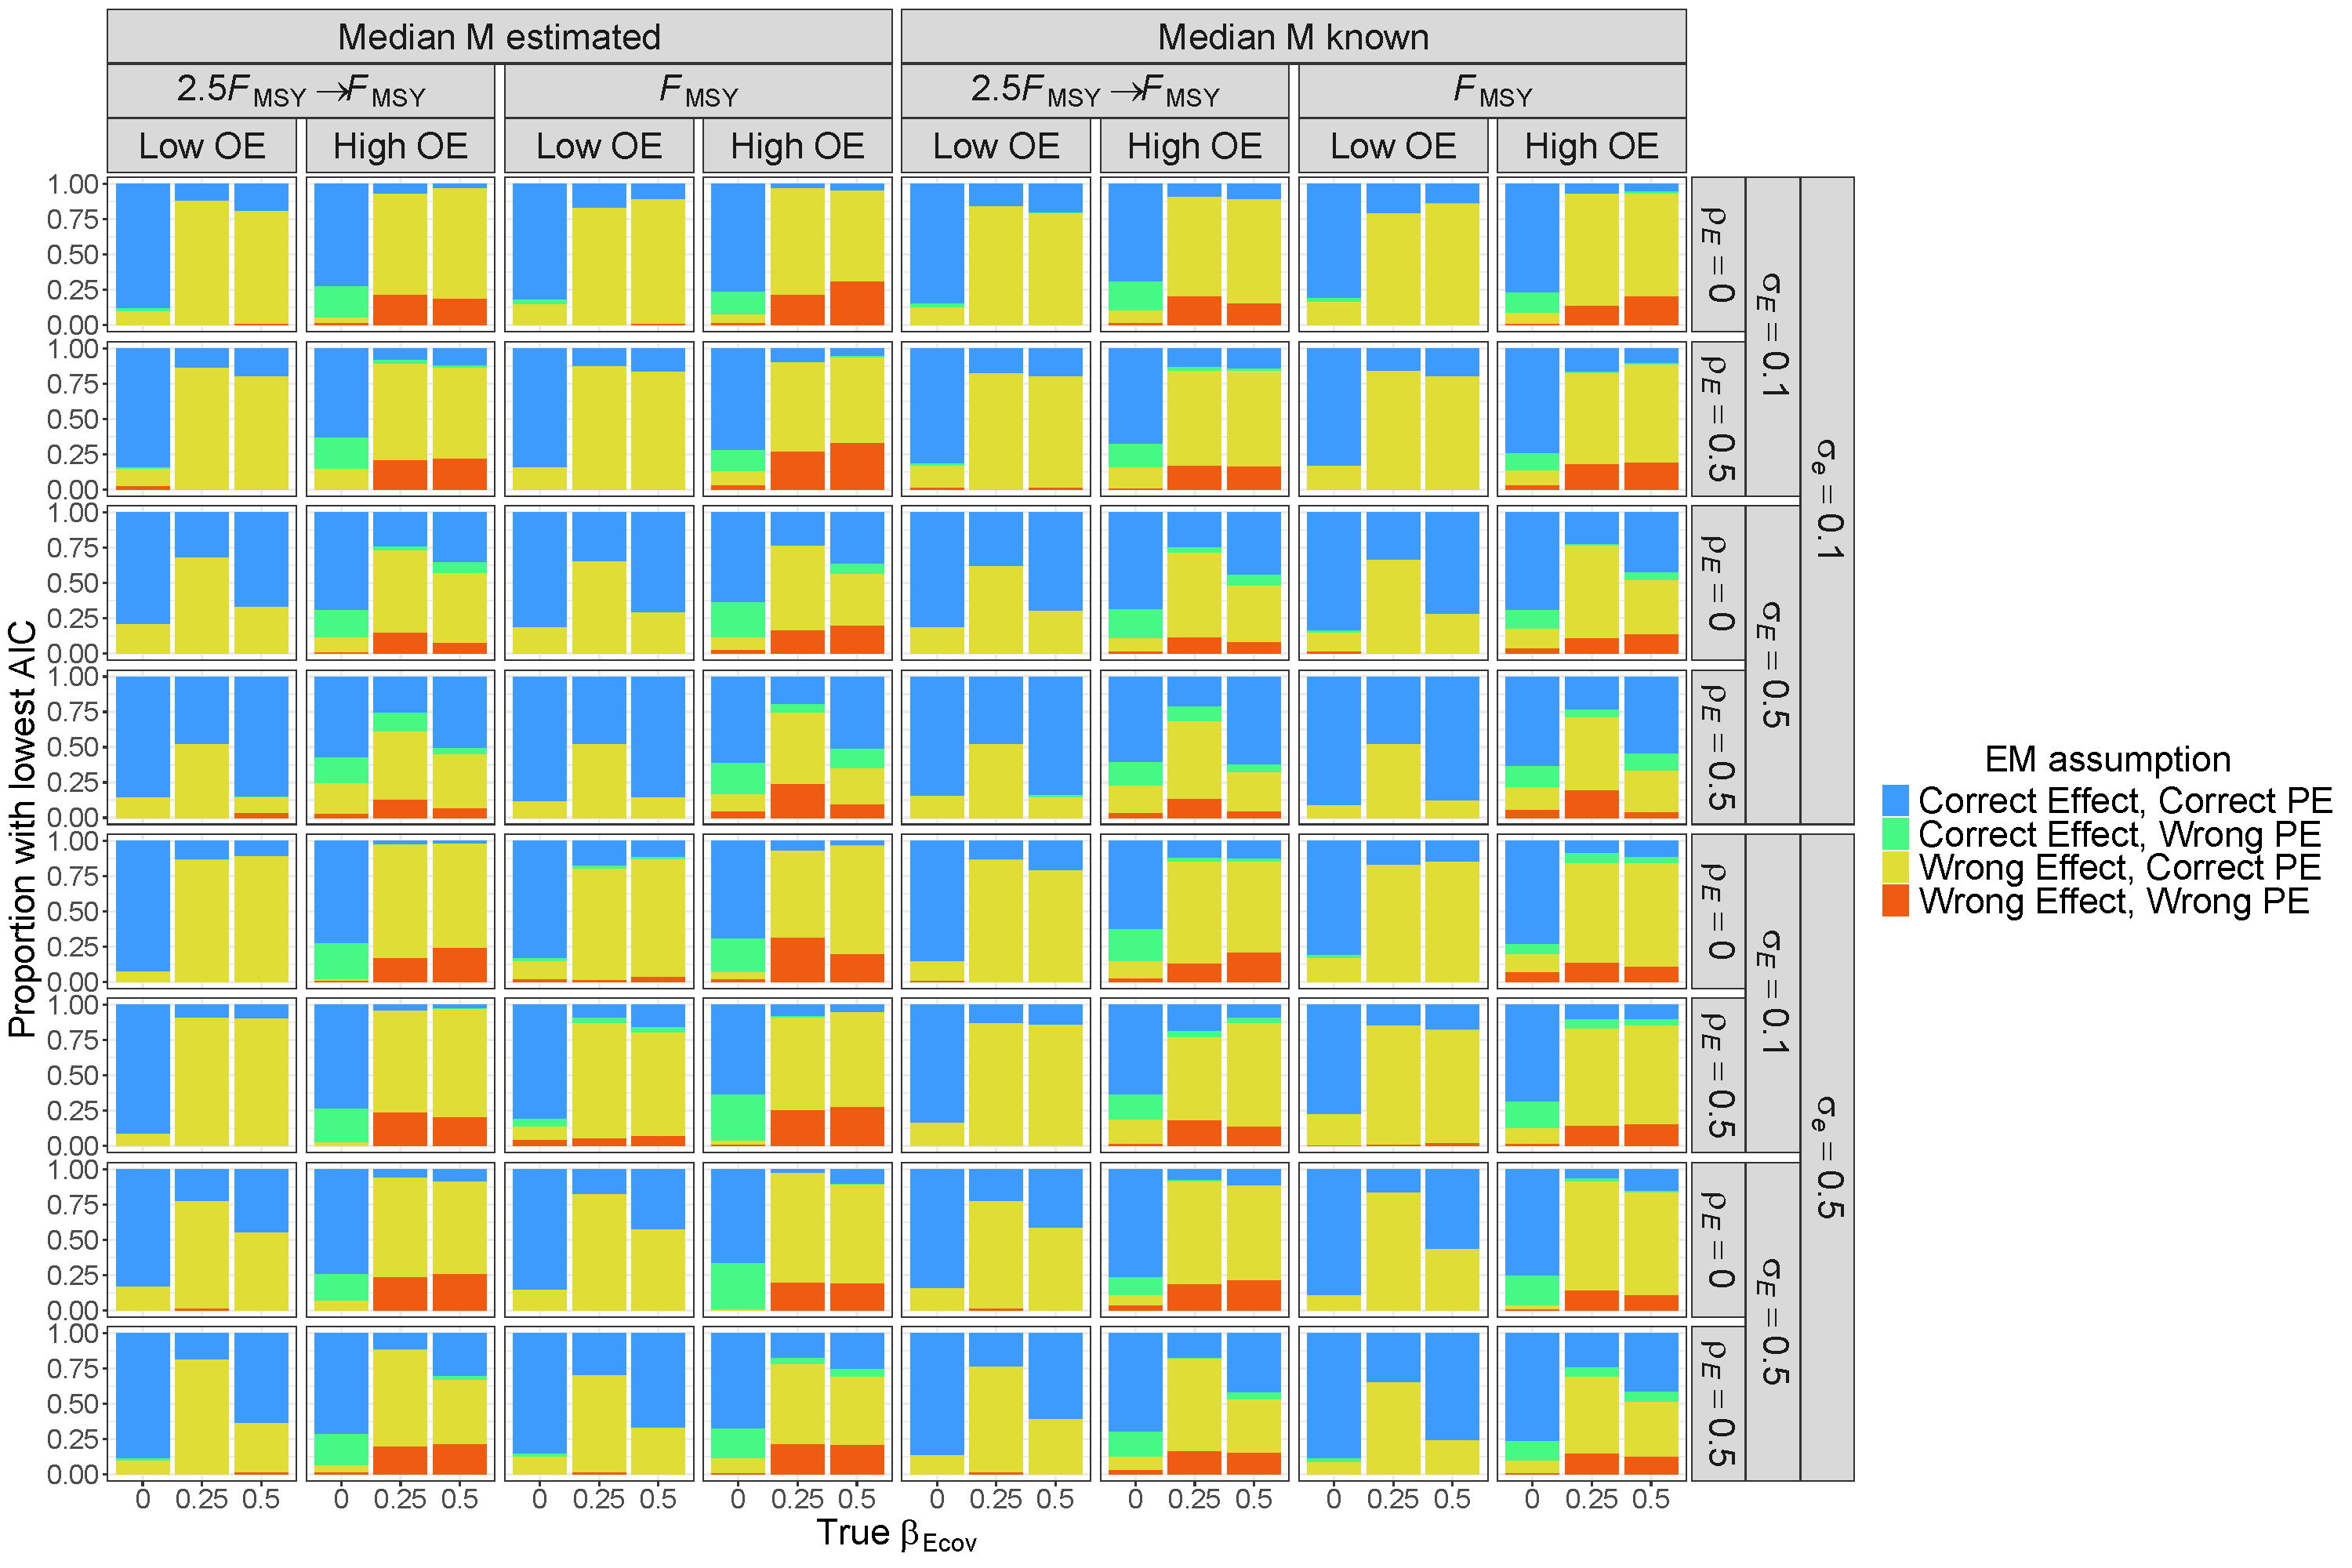
\includegraphics[height = \textheight]{aic_RSom}
\end{center}
\caption{Proportion of simulated data sets for R+S OMs where the EM type (treatment of environmental covariate and assumed process error type) had the lowest AIC.}\label{aic_RSom}
\end{figure}
\end{landscape}

\begin{landscape}
\begin{figure}
\begin{center}
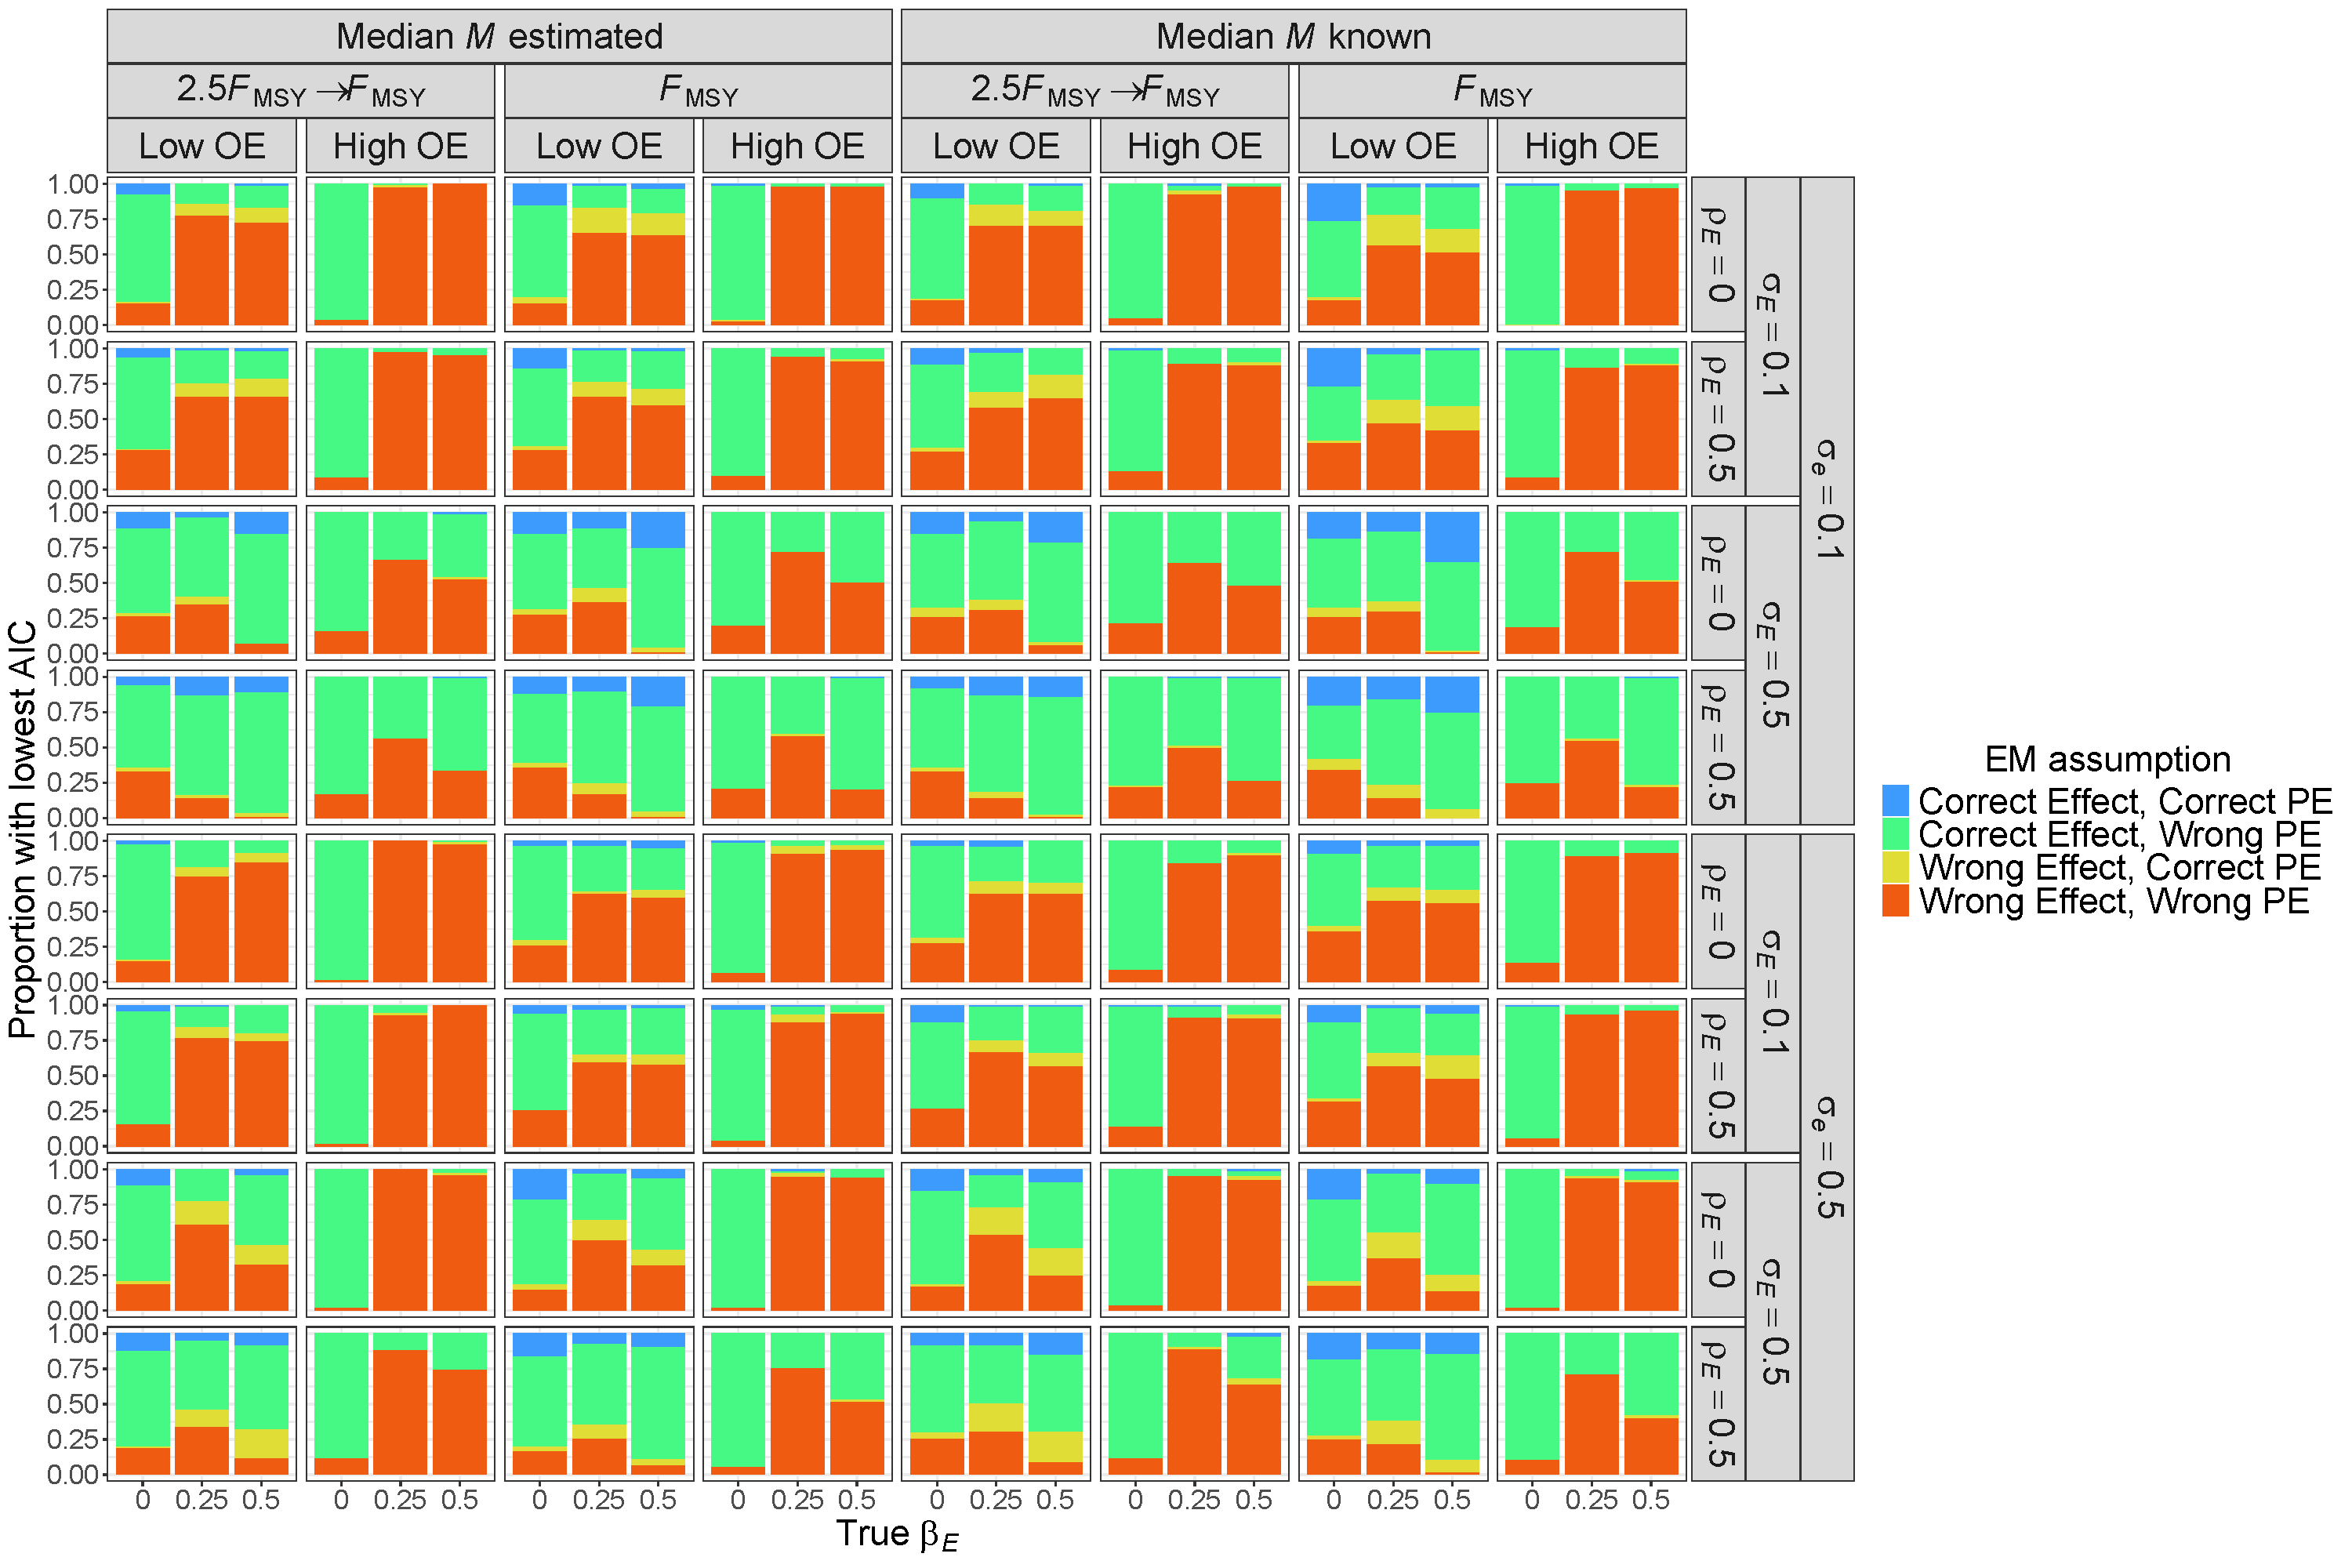
\includegraphics[height = \textheight]{aic_RMom}
\end{center}
\caption{Proportion of simulated data sets for R+M OMs where the EM type (treatment of environmental covariate and assumed process error type) had the lowest AIC.}\label{aic_RMom}
\end{figure}
\end{landscape}

\DIFdelbegin %DIFDELCMD < \hypertarget{covariate-effect-bias}{%
%DIFDELCMD < \subsection*{Covariate effect bias}\label{covariate-effect-bias}}
%DIFDELCMD < %%%
\DIFdelend \DIFaddbegin \subsection*{\DIFadd{Covariate effect bias}}\label{covariate-effect-bias}
\DIFaddend \addcontentsline{toc}{subsection}{Covariate effect bias}

\DIFaddbegin \begin{table}
\caption{\DIFaddFL{For each OM process error source (columns), percent reduction in deviance for linear regression models fit to errors in estimation of the covariate effect on $M$ ($\beta_E$) with each OM and EM factor (rows) included individually, combined, and with second and third order interactions. Includes results from all unconverged and converged models.}}\label{bias_ecov_beta_complete_PRD_table}
{\begin{center}
\begin{tabular}{lrrr}
\hline\hline
\multicolumn{1}{l}{\DIFaddFL{Factor}}&\multicolumn{1}{c}{\DIFaddFL{R}}&\multicolumn{1}{c}{\DIFaddFL{R+S}}&\multicolumn{1}{c}{\DIFaddFL{R+M}}\tabularnewline
\hline
\DIFaddFL{OM $F$ history}&\DIFaddFL{\textless  0.01}&\DIFaddFL{0.01}&\DIFaddFL{\textless  0.01}\tabularnewline
\DIFaddFL{OM Obs. Error}&\DIFaddFL{\textless  0.01}&\DIFaddFL{\textless  0.01}&\DIFaddFL{\textless  0.01}\tabularnewline
\DIFaddFL{OM $\sigma_e$}&\DIFaddFL{\textless  0.01}&\DIFaddFL{\textless  0.01}&\DIFaddFL{\textless  0.01}\tabularnewline
\DIFaddFL{OM $\sigma_E$}&\DIFaddFL{\textless  0.01}&\DIFaddFL{\textless  0.01}&\DIFaddFL{\textless  0.01}\tabularnewline
\DIFaddFL{OM $\rho_{E}$}&\DIFaddFL{\textless  0.01}&\DIFaddFL{\textless  0.01}&\DIFaddFL{\textless  0.01}\tabularnewline
\DIFaddFL{OM $\beta_{E}$}&\DIFaddFL{\textless  0.01}&\DIFaddFL{0.01}&\DIFaddFL{\textless  0.01}\tabularnewline
\DIFaddFL{EM Convergence}&\DIFaddFL{\textless  0.01}&\DIFaddFL{\textless  0.01}&\DIFaddFL{\textless  0.01}\tabularnewline
\DIFaddFL{EM Process Error}&\DIFaddFL{\textless  0.01}&\DIFaddFL{0.01}&\DIFaddFL{0.01}\tabularnewline
\DIFaddFL{EM $M$ assumption}&\DIFaddFL{\textless  0.01}&\DIFaddFL{\textless  0.01}&\DIFaddFL{\textless  0.01}\tabularnewline
\DIFaddFL{All factors}&\DIFaddFL{0.02}&\DIFaddFL{0.03}&\DIFaddFL{0.03}\tabularnewline
\DIFaddFL{+ All Two Way}&\DIFaddFL{0.16}&\DIFaddFL{0.20}&\DIFaddFL{0.18}\tabularnewline
\DIFaddFL{+ All Three Way}&\DIFaddFL{0.58}&\DIFaddFL{0.73}&\DIFaddFL{0.59}\tabularnewline
\hline
\end{tabular}\end{center}
}
\end{table}

\DIFaddend \begin{landscape}
\begin{figure}
\begin{center}
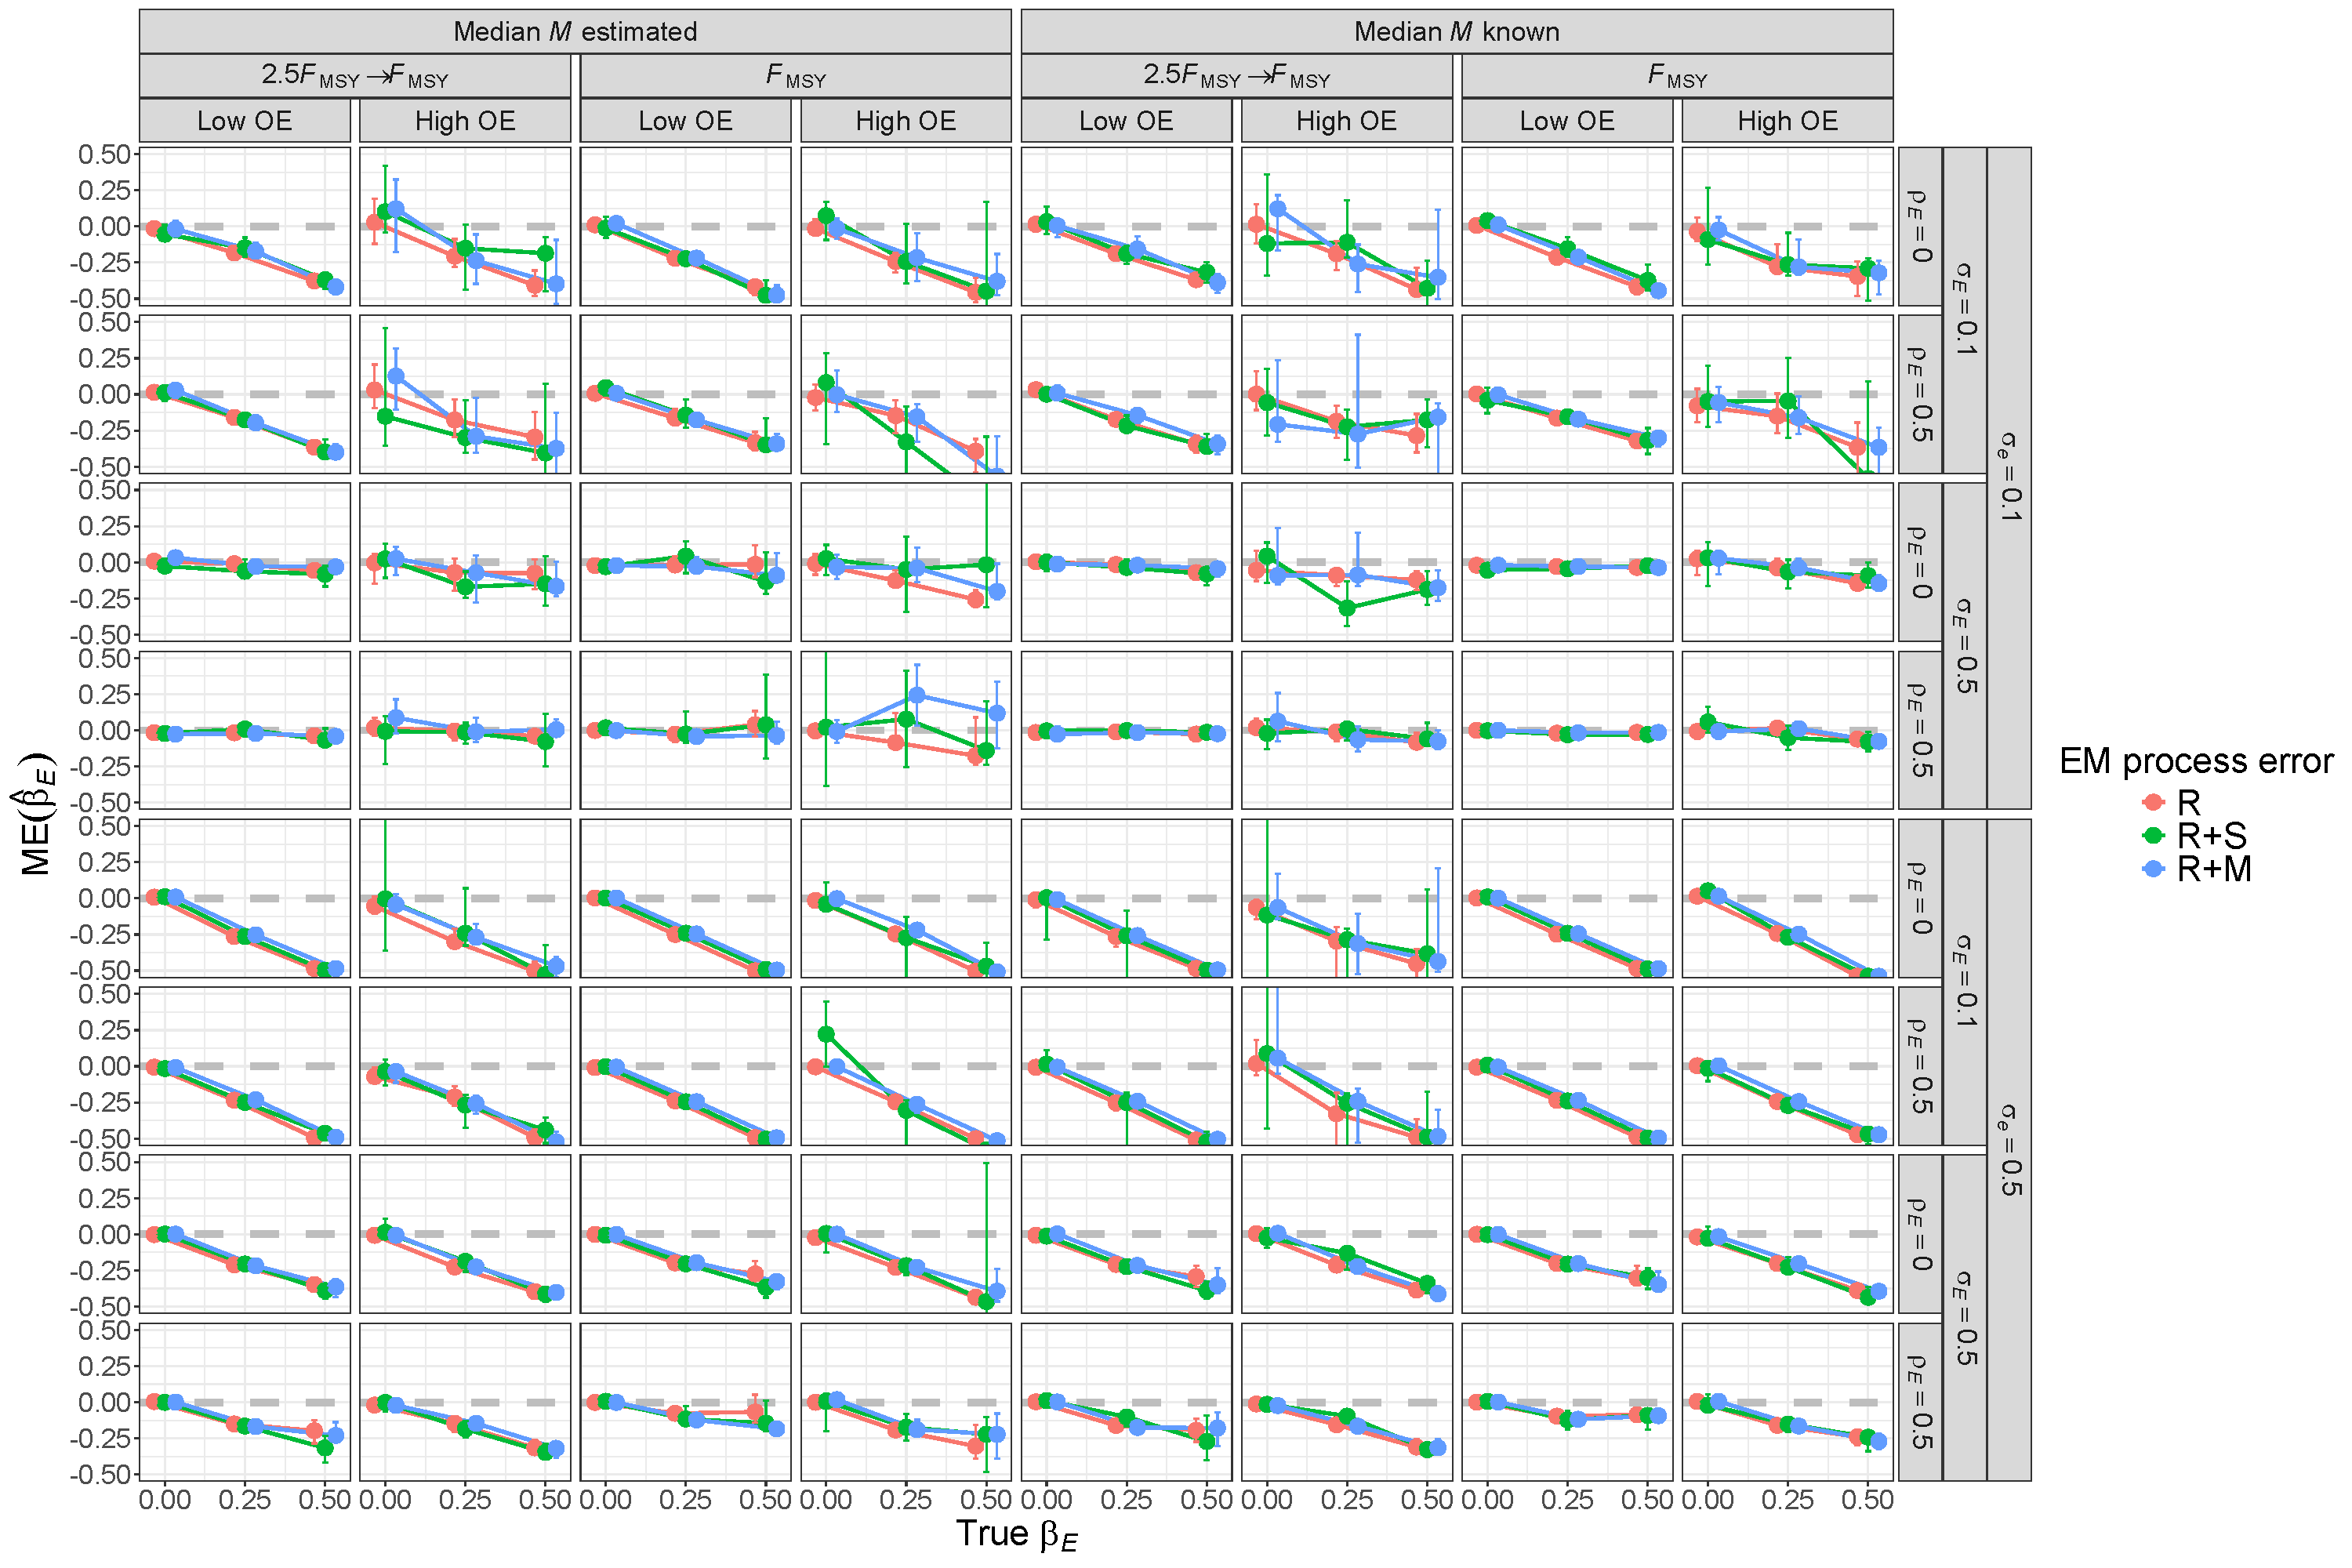
\includegraphics[height = \textheight]{beta_E_bias_Rom}
\end{center}
\caption{For R OMs, median error (ME) of estimates of environmental effect on \DIFdelbeginFL \DIFdelFL{natural mortality }\DIFdelendFL \DIFaddbeginFL \DIFaddFL{$M$ (}\DIFaddendFL $\beta_E$\DIFaddbeginFL \DIFaddFL{) }\DIFaddendFL from fitting EMs with alternative process error assumptions and treatment of median \DIFdelbeginFL \DIFdelFL{natural mortality }\DIFdelendFL \DIFaddbeginFL \DIFaddFL{$M$ }\DIFaddendFL ($e^\beta_M$ known or estimated). Vertical lines represent 95\% confidence intervals.}\label{beta_E_bias_Rom}
\end{figure}
\end{landscape}

\begin{landscape}
\begin{figure}
\begin{center}
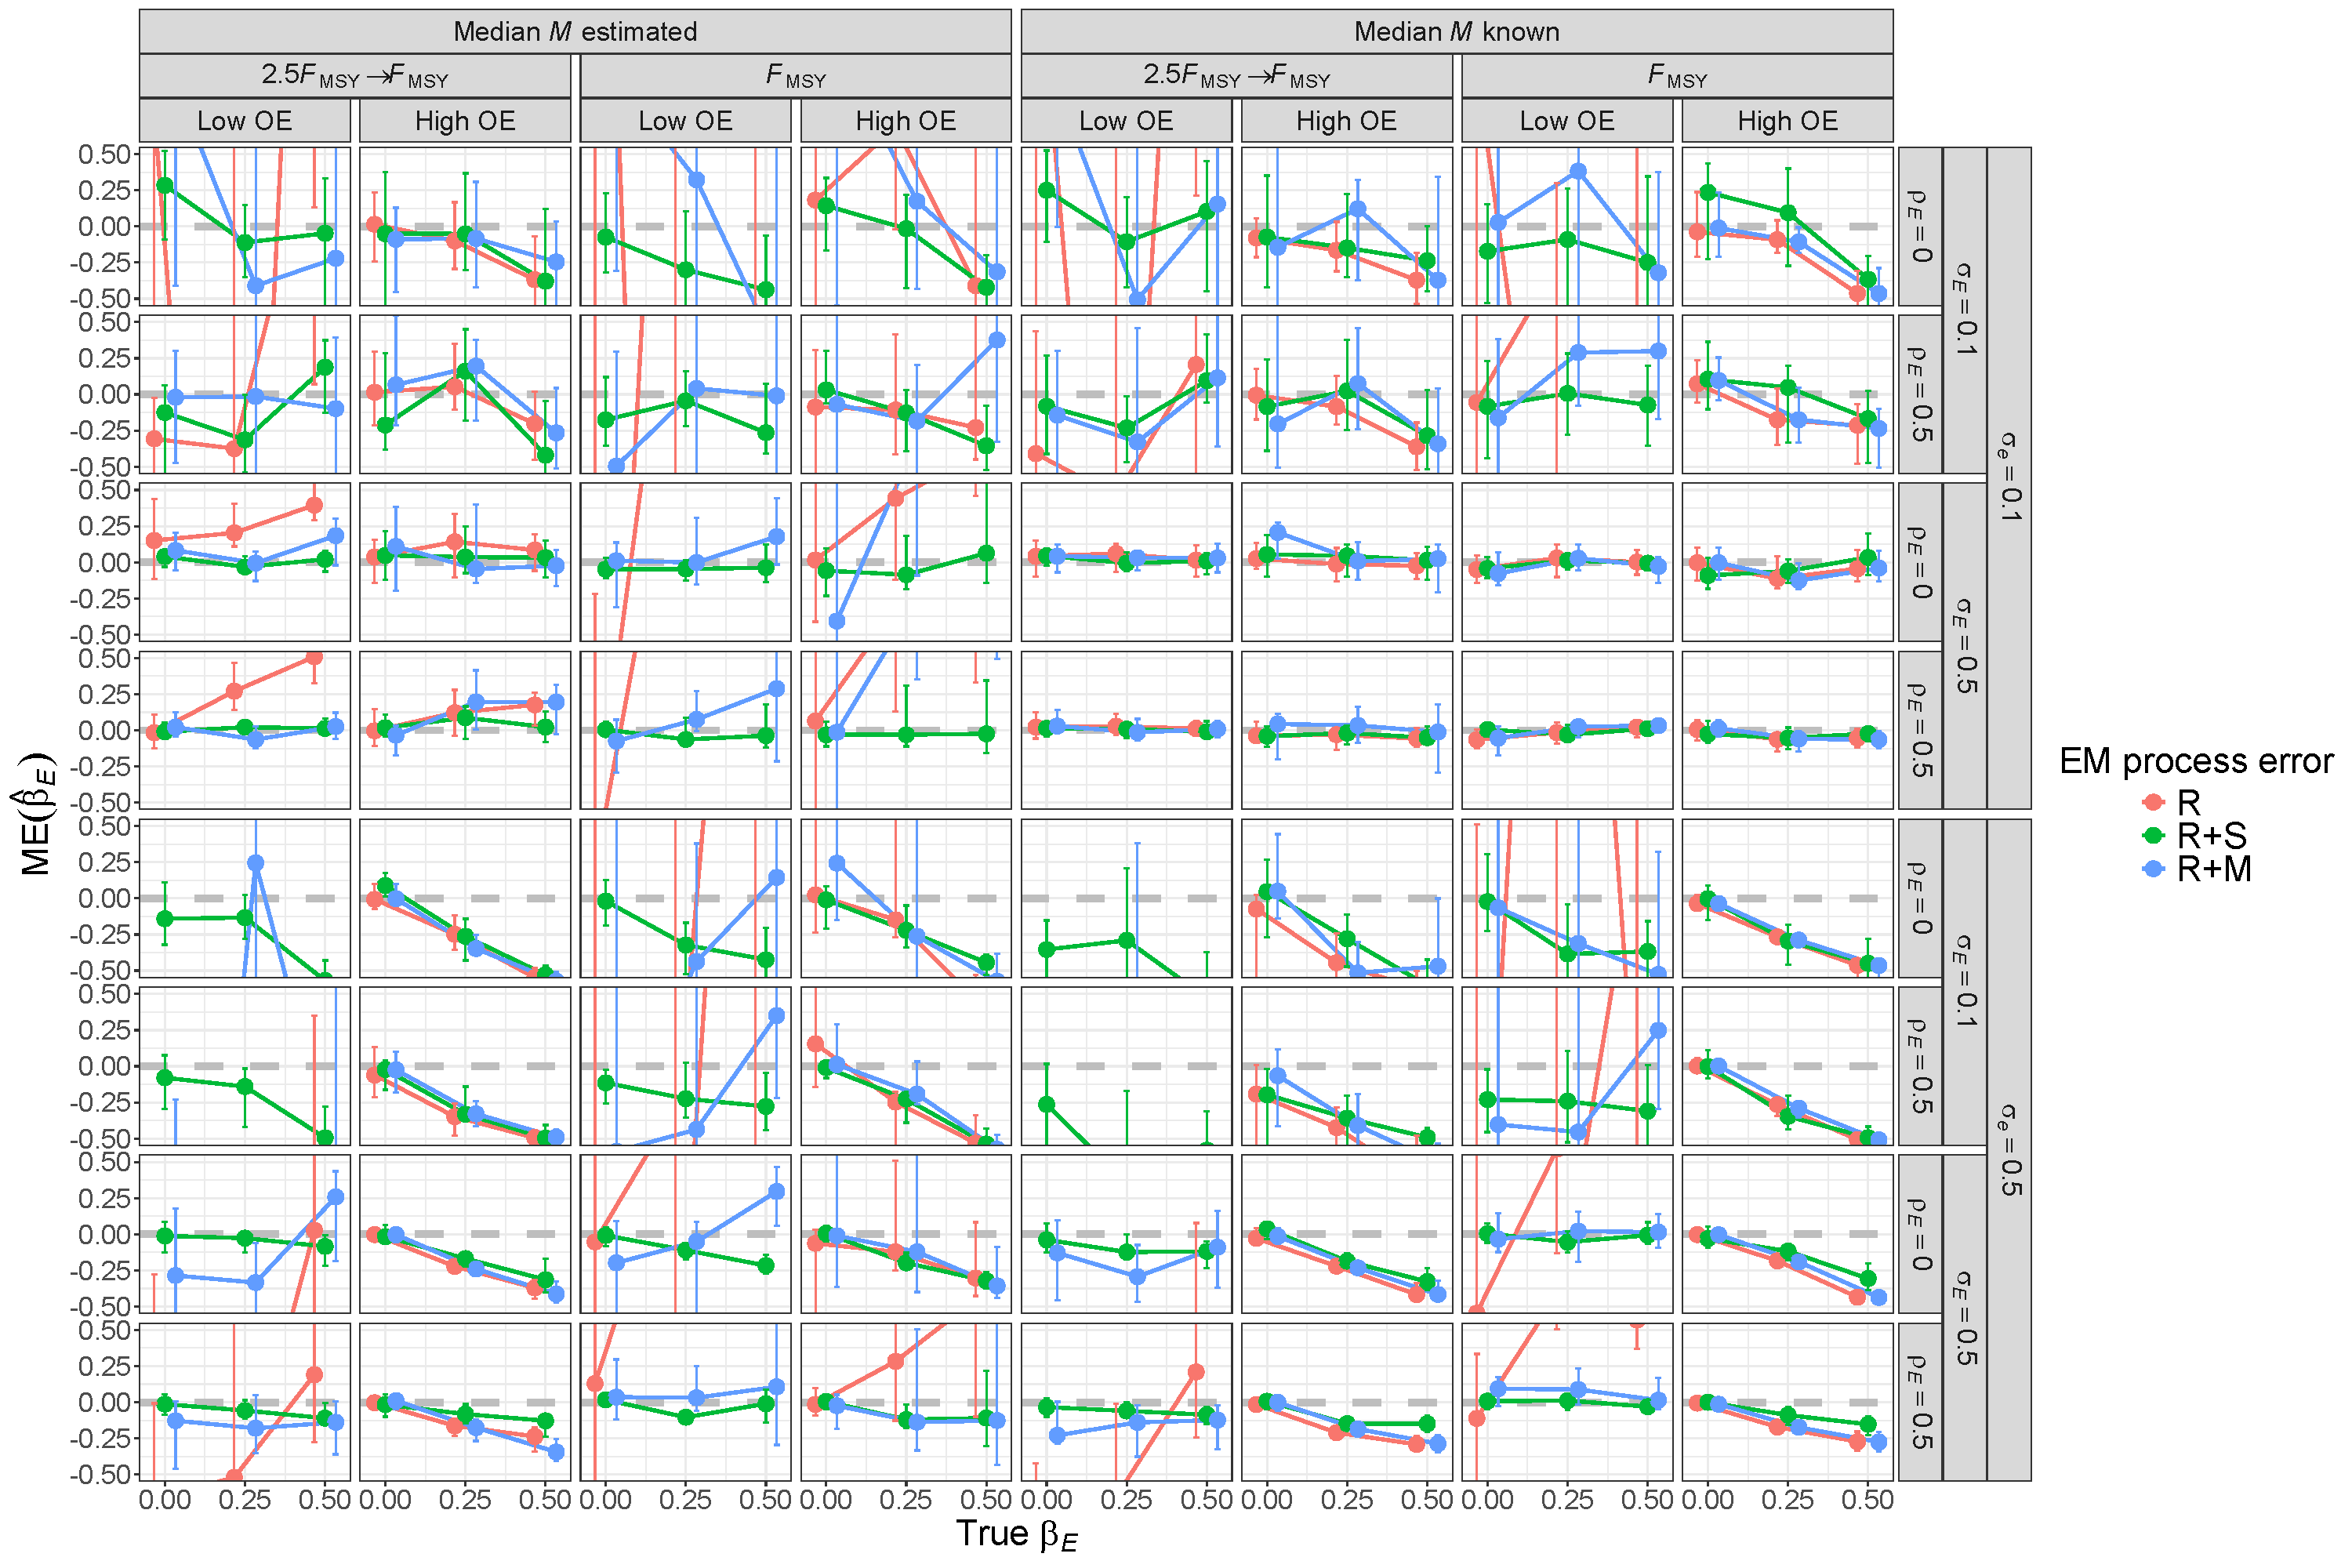
\includegraphics[height = \textheight]{beta_E_bias_RSom}
\end{center}
\caption{For R+S OMs, median error (ME) of estimates of environmental effect on \DIFdelbeginFL \DIFdelFL{natural mortality }\DIFdelendFL \DIFaddbeginFL \DIFaddFL{$M$ (}\DIFaddendFL $\beta_E$\DIFaddbeginFL \DIFaddFL{) }\DIFaddendFL from fitting EMs with alternative process error assumptions and treatment of median \DIFdelbeginFL \DIFdelFL{natural mortality }\DIFdelendFL \DIFaddbeginFL \DIFaddFL{$M$ }\DIFaddendFL ($e^\beta_M$ known or estimated). Vertical lines represent 95\% confidence intervals.}\label{beta_E_bias_RSom}
\end{figure}
\end{landscape}

\begin{landscape}
\begin{figure}
\begin{center}
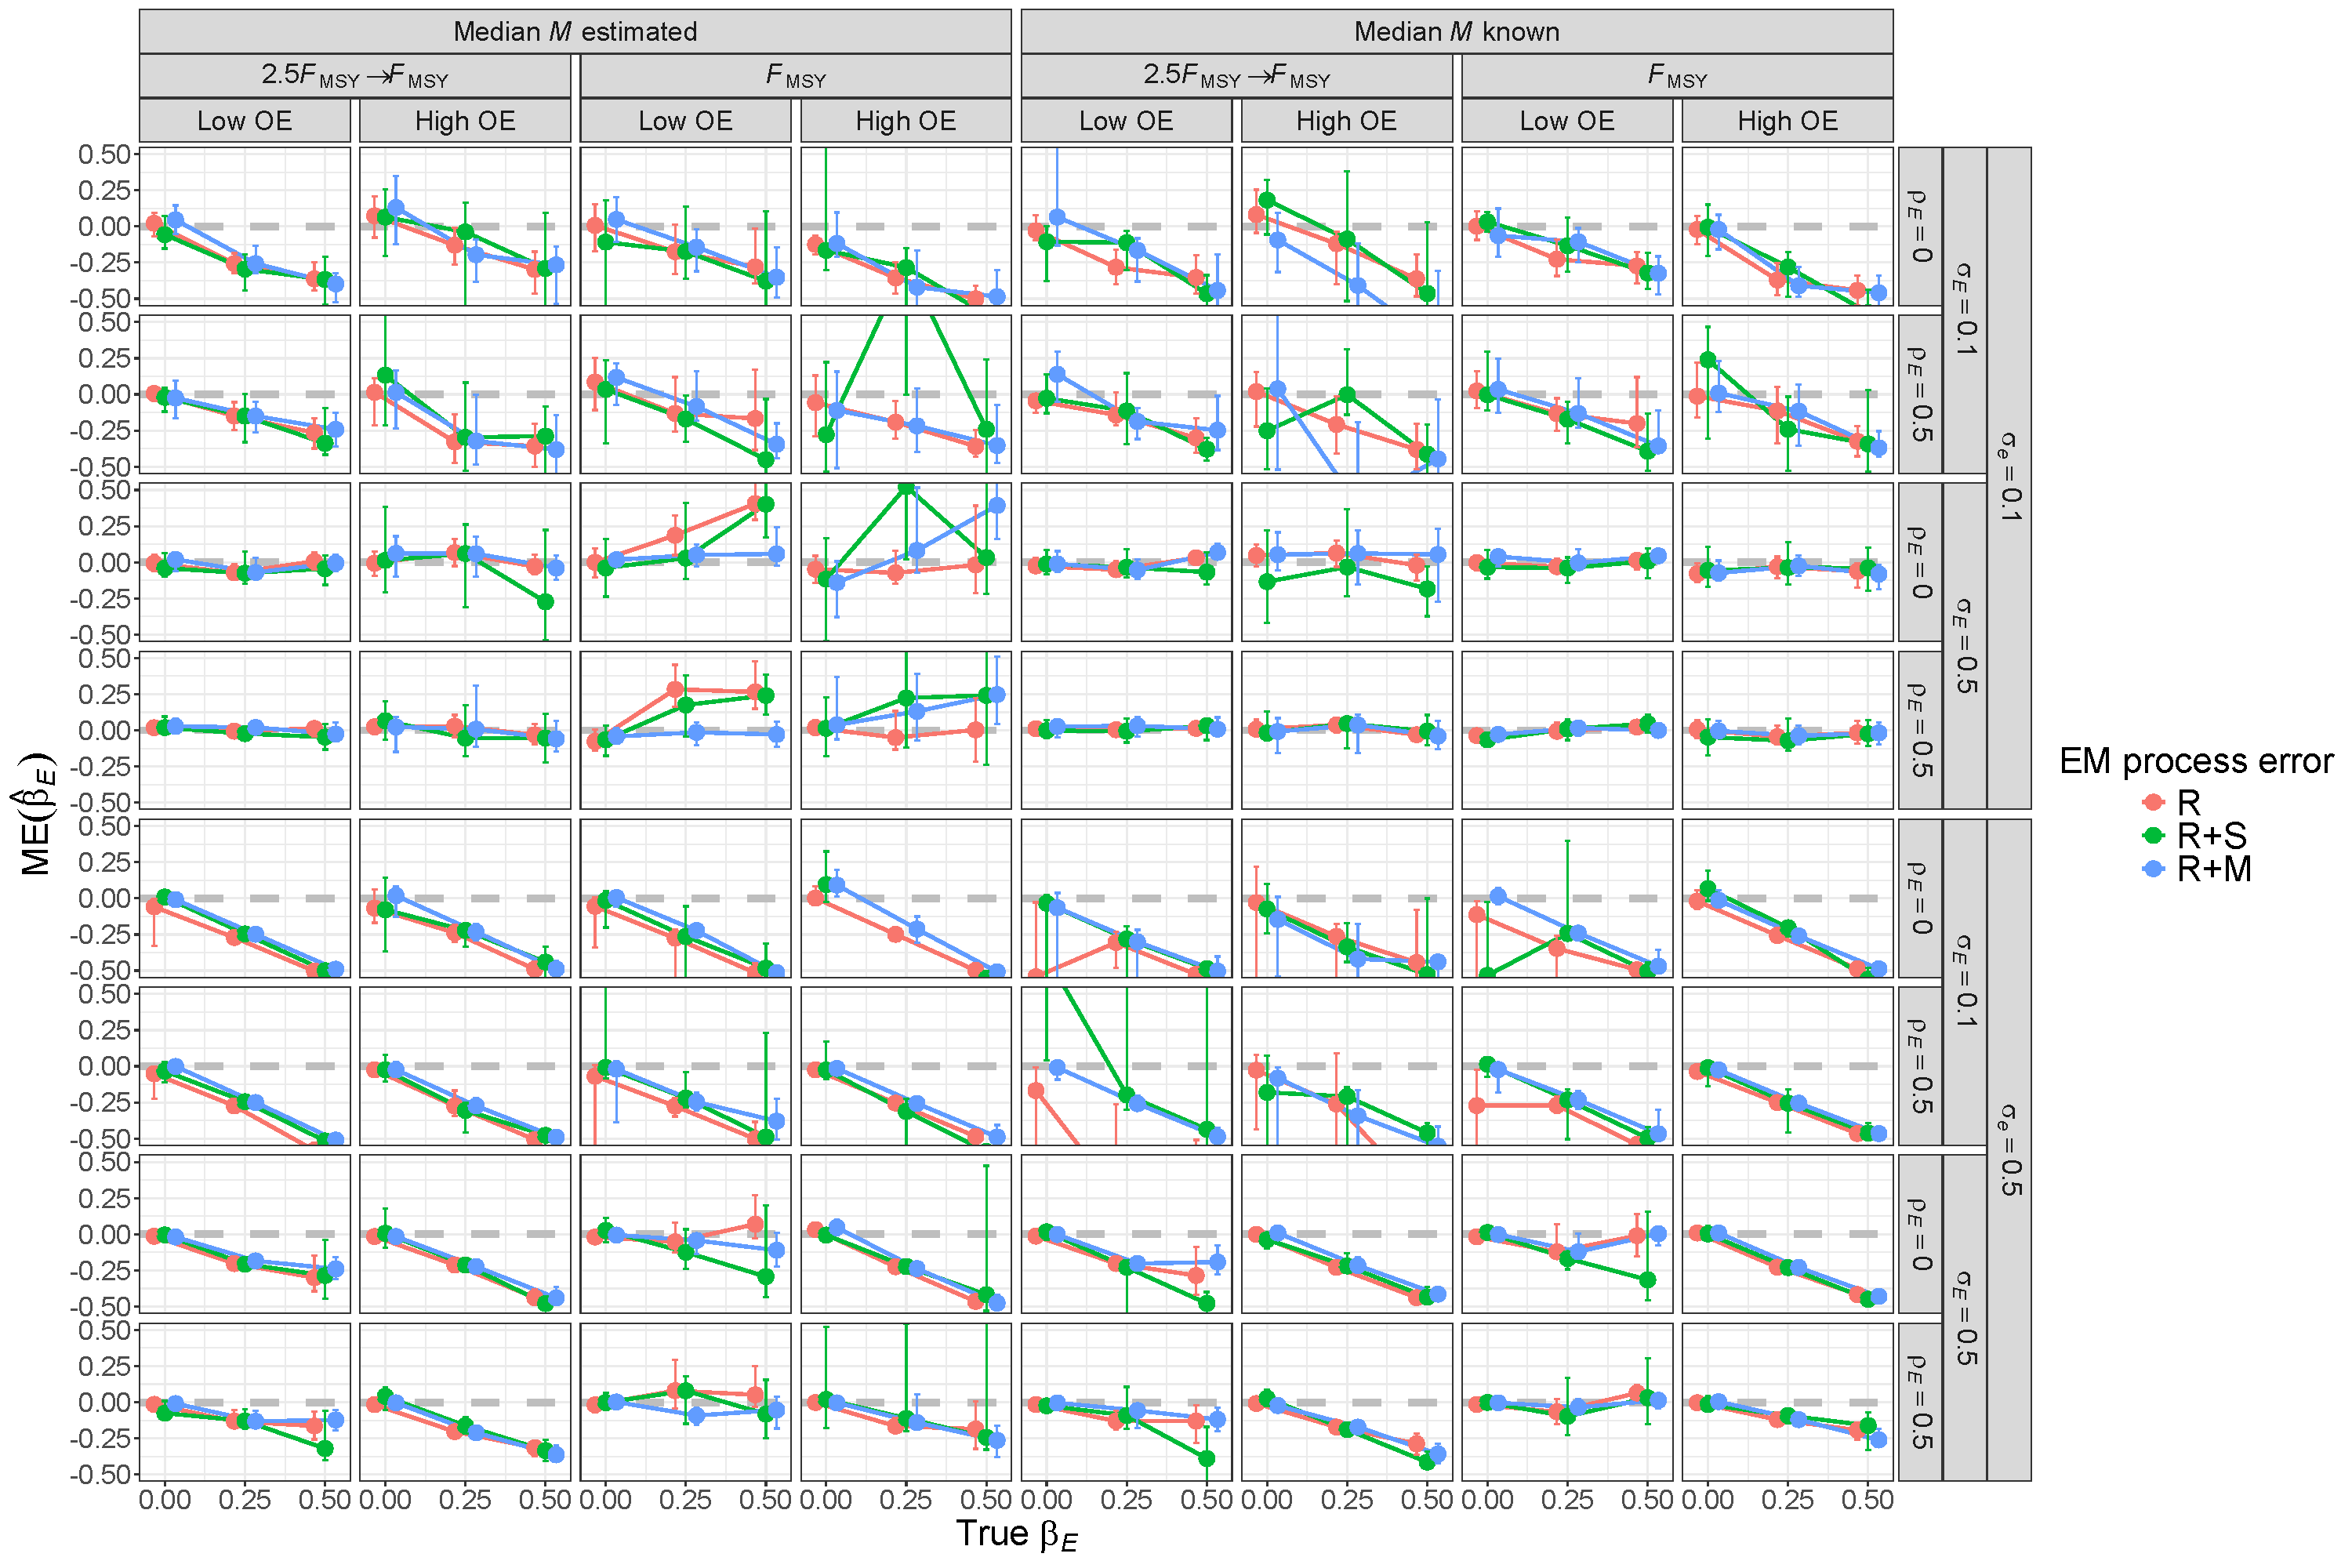
\includegraphics[height = \textheight]{beta_E_bias_RMom}
\end{center}
\caption{For R+M OMs, median error (ME) of estimates of environmental effect on \DIFdelbeginFL \DIFdelFL{natural mortality }\DIFdelendFL \DIFaddbeginFL \DIFaddFL{$M$ (}\DIFaddendFL $\beta_E$\DIFaddbeginFL \DIFaddFL{) }\DIFaddendFL from fitting EMs with alternative process error assumptions and treatment of median \DIFdelbeginFL \DIFdelFL{natural mortality }\DIFdelendFL \DIFaddbeginFL \DIFaddFL{$M$ }\DIFaddendFL ($e^\beta_M$ known or estimated). Vertical lines represent 95\% confidence intervals.}\label{beta_E_bias_RMom}
\end{figure}
\end{landscape}

\DIFdelbegin %DIFDELCMD < \hypertarget{covariate-effect-standard-error-estimation-bias}{%
%DIFDELCMD < \subsection*{Covariate effect standard error estimation bias}\label{covariate-effect-standard-error-estimation-bias}}
%DIFDELCMD < %%%
\DIFdelend \DIFaddbegin \subsection*{\DIFadd{Covariate effect standard error estimation bias}}\label{covariate-effect-standard-error-estimation-bias}
\DIFaddend \addcontentsline{toc}{subsection}{Covariate effect standard error estimation bias}

\begin{landscape}
\begin{figure}
\begin{center}
\DIFdelbeginFL %DIFDELCMD < 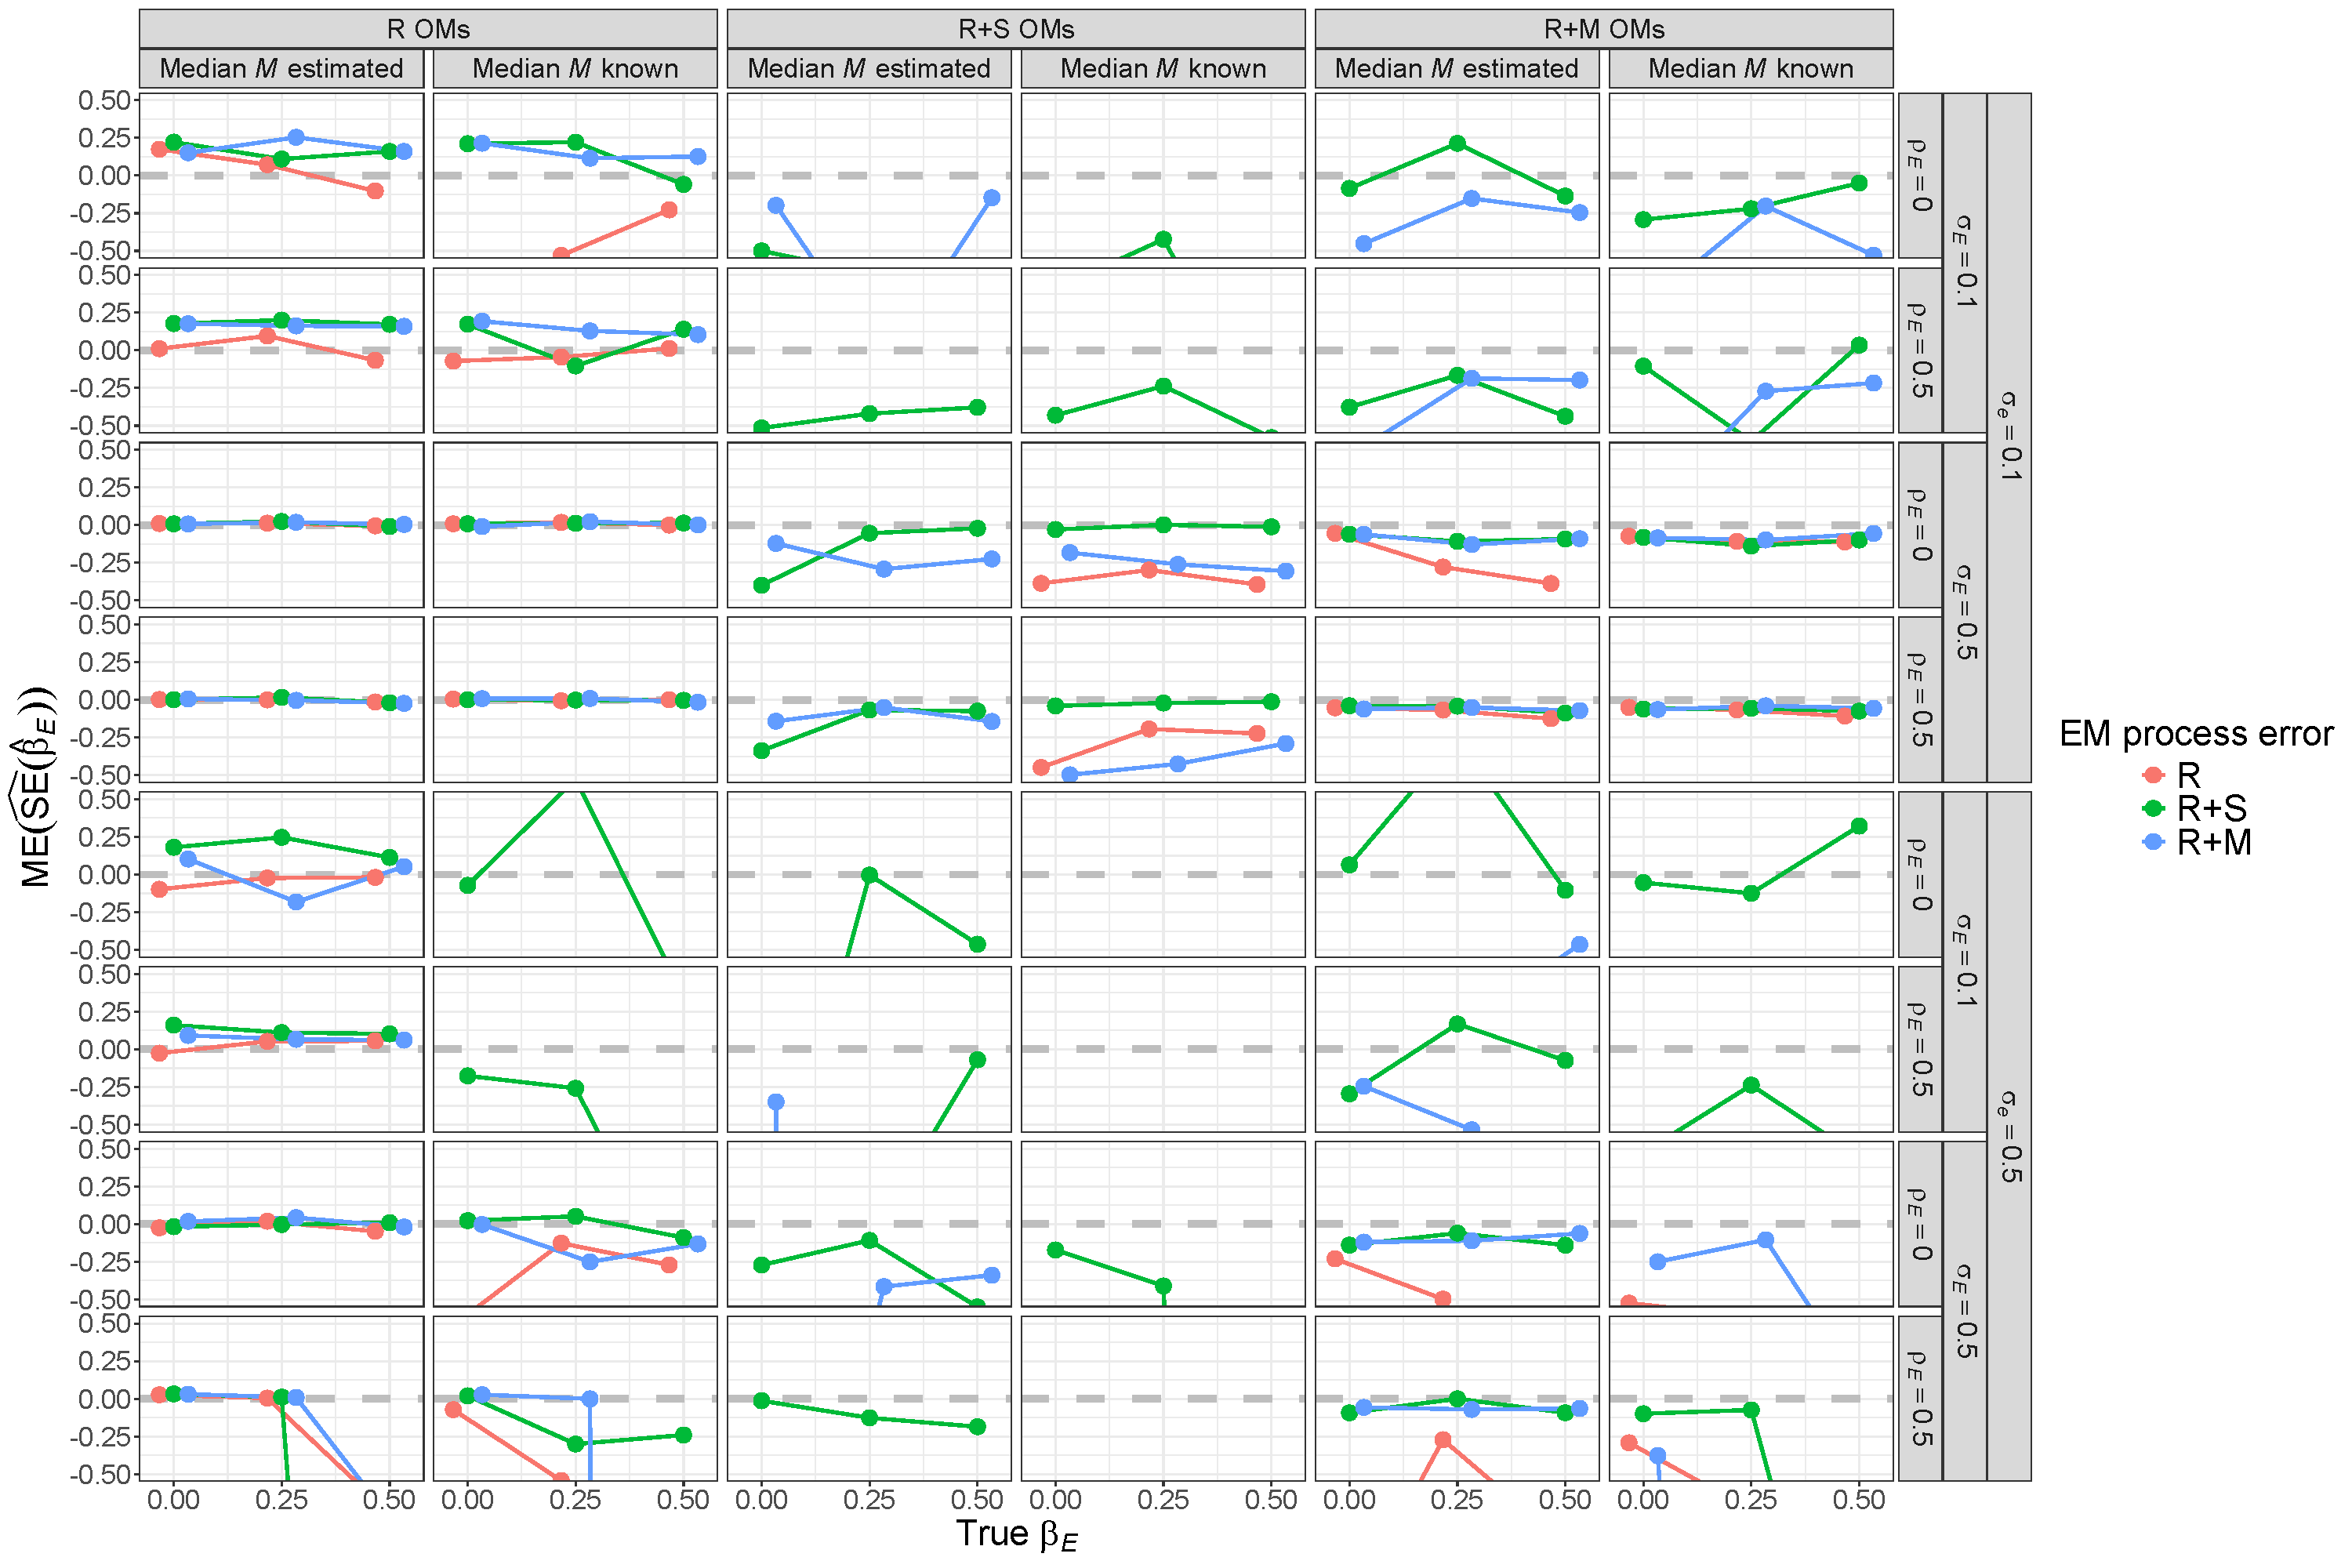
\includegraphics[height = \textheight]{se_beta_E_bias_main}
%DIFDELCMD < \end{center}
%DIFDELCMD < %%%
%DIFDELCMD < \caption{%
{%DIFAUXCMD
\DIFdelFL{Median error (ME) of Hessian-based estimates of standard error for covariate effect on natural mortality $\beta_E$ from fitting EMs with alternative process error assumptions and treatment of median natural mortality ($e^\beta_M$ known or estimated). All OMs had low observation error and contrast in fishing mortality. True standard error is defined as the mean of the standard error estimates accross converged fits to simulated data sets for a given OM scenario.}}%DIFAUXCMD
%DIFDELCMD < \label{se_beta_E_bias}
%DIFDELCMD < \end{figure}
%DIFDELCMD < \end{landscape}
%DIFDELCMD < 

%DIFDELCMD < \begin{landscape}
%DIFDELCMD < \begin{figure}
%DIFDELCMD < \begin{center}
%DIFDELCMD < %%%
\DIFdelendFL 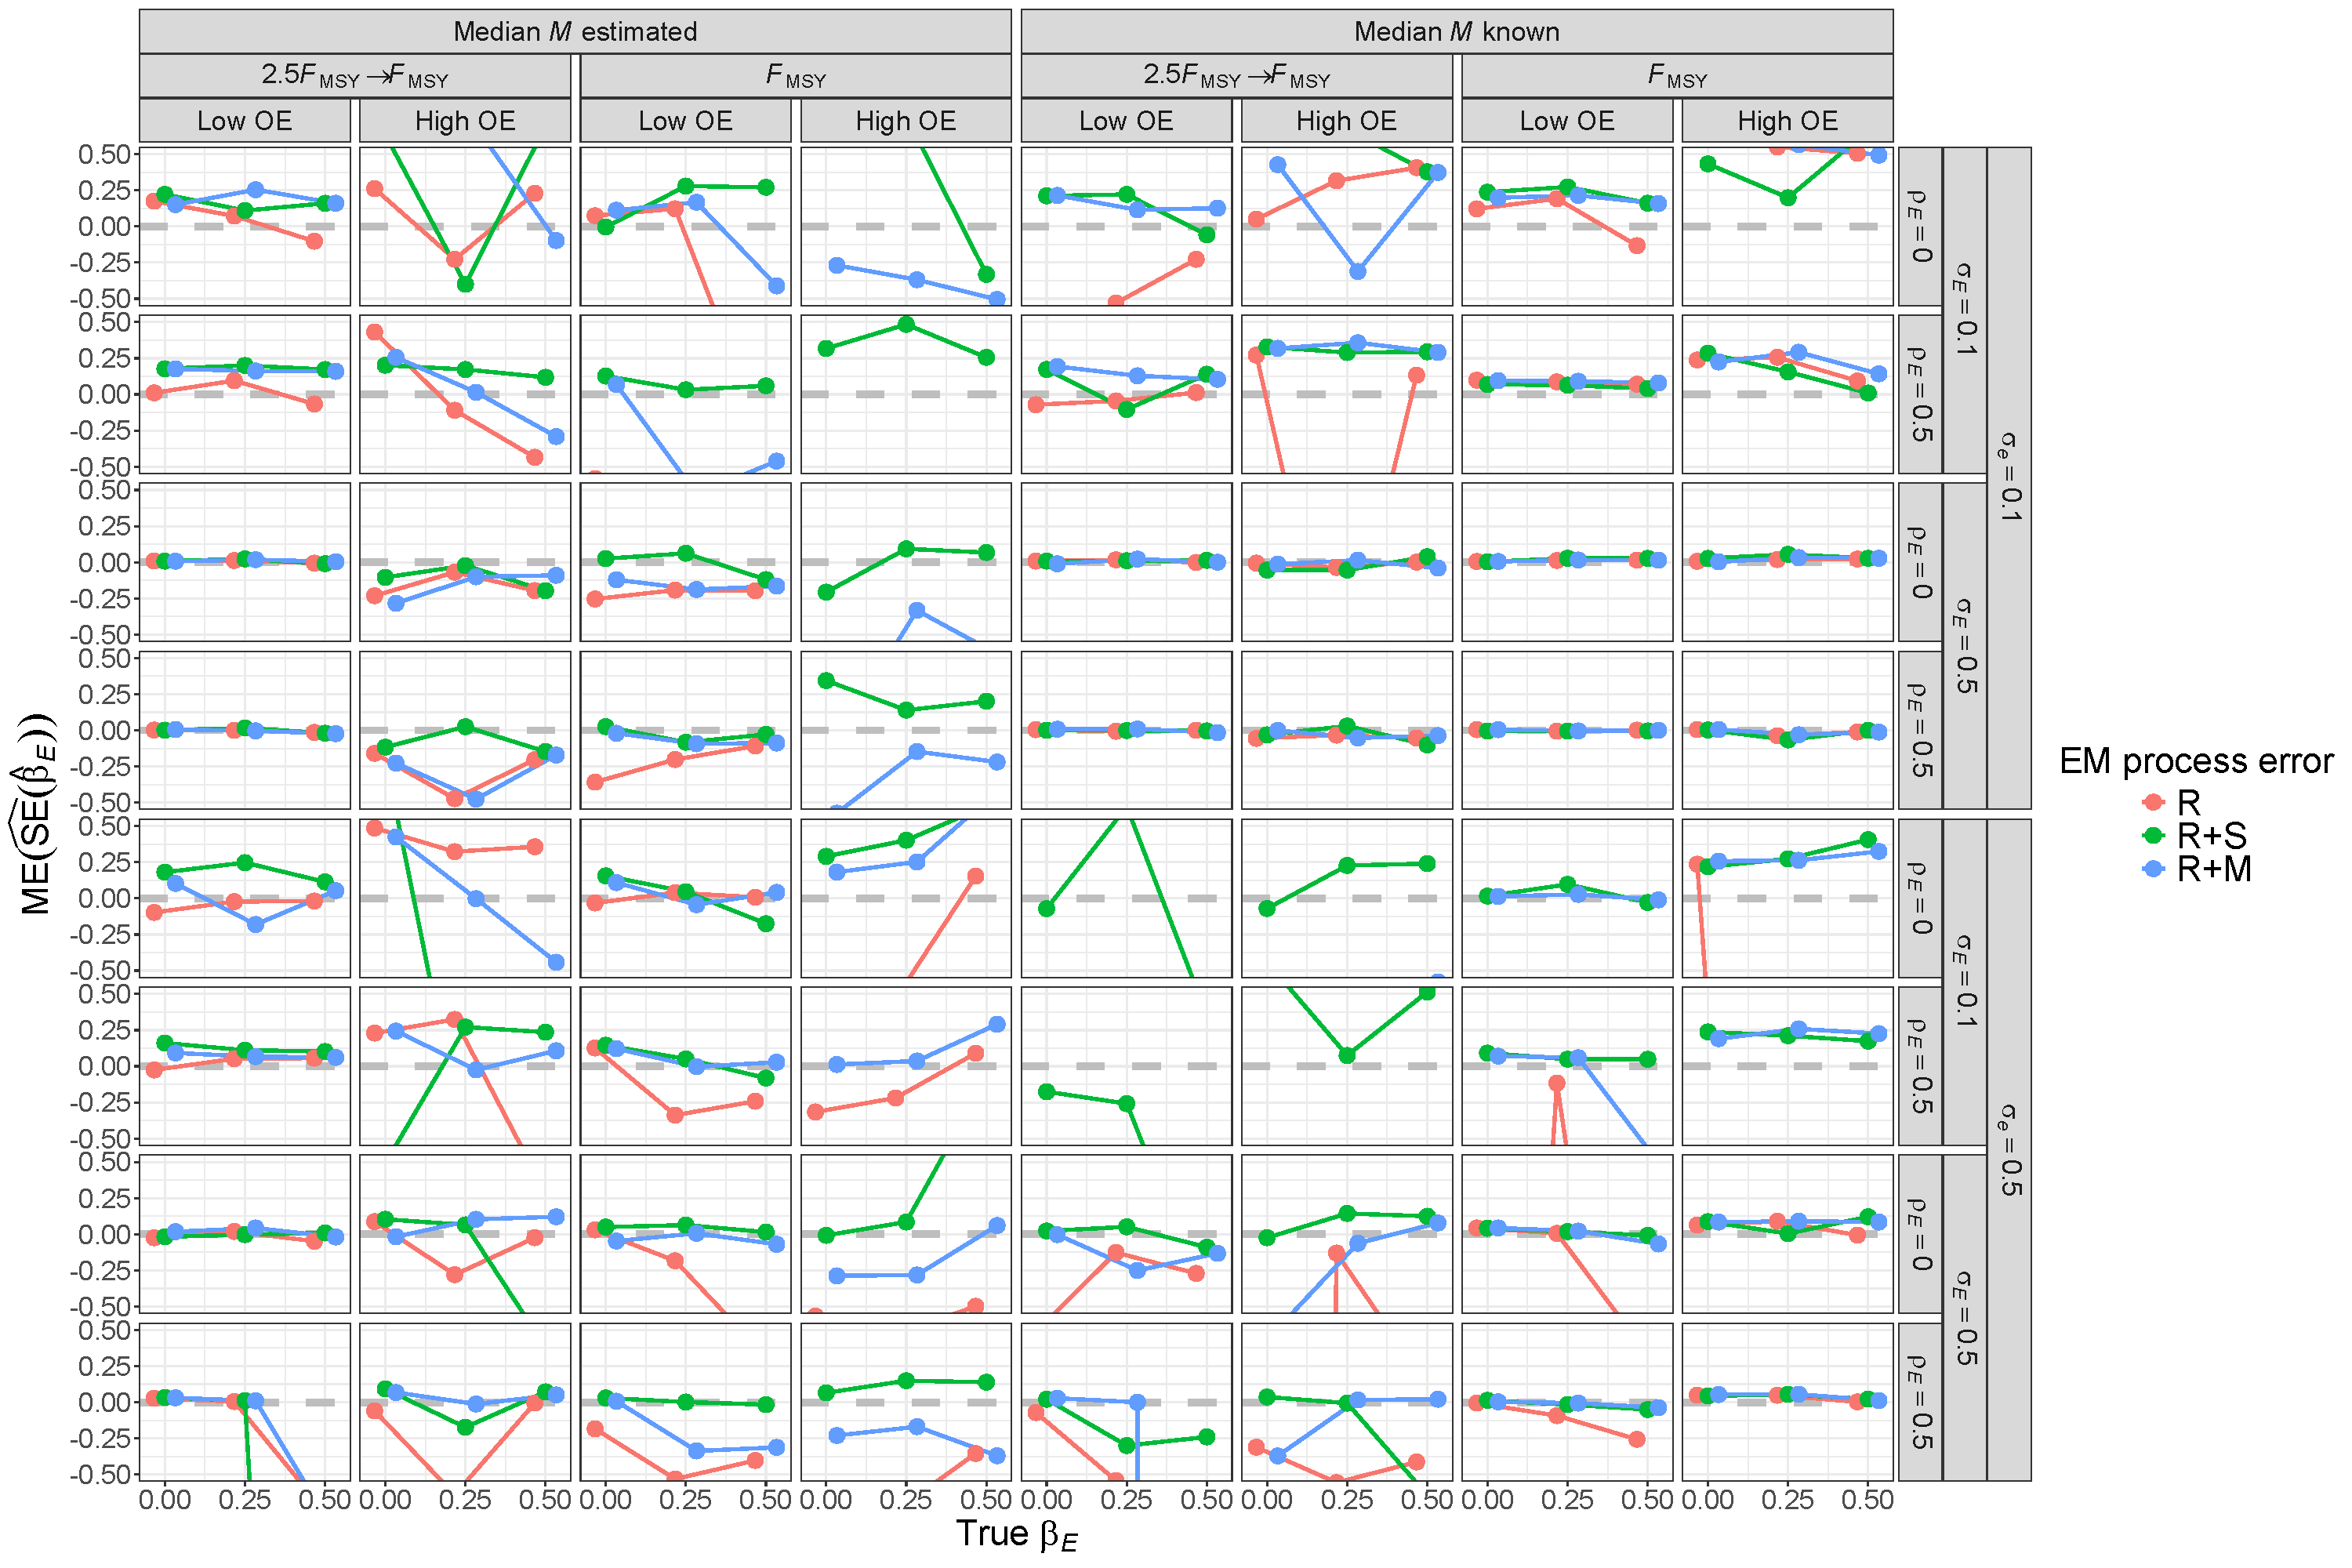
\includegraphics[height = \textheight]{se_beta_E_bias_Rom}
\end{center}
\caption{For R OMs, median error (ME) of Hessian-based estimates of standard error for covariate effect on \DIFdelbeginFL \DIFdelFL{natural mortality }\DIFdelendFL \DIFaddbeginFL \DIFaddFL{$M$ (}\DIFaddendFL $\beta_E$\DIFaddbeginFL \DIFaddFL{) }\DIFaddendFL from fitting EMs with alternative process error assumptions and treatment of median \DIFdelbeginFL \DIFdelFL{natural mortality }\DIFdelendFL \DIFaddbeginFL \DIFaddFL{$M$ }\DIFaddendFL ($e^\beta_M$ known or estimated). True standard error is defined as the mean of the standard error estimates accross converged fits to simulated data sets for a given OM scenario.}\label{se_beta_E_bias_Rom}
\end{figure}
\end{landscape}

\begin{landscape}
\begin{figure}
\begin{center}
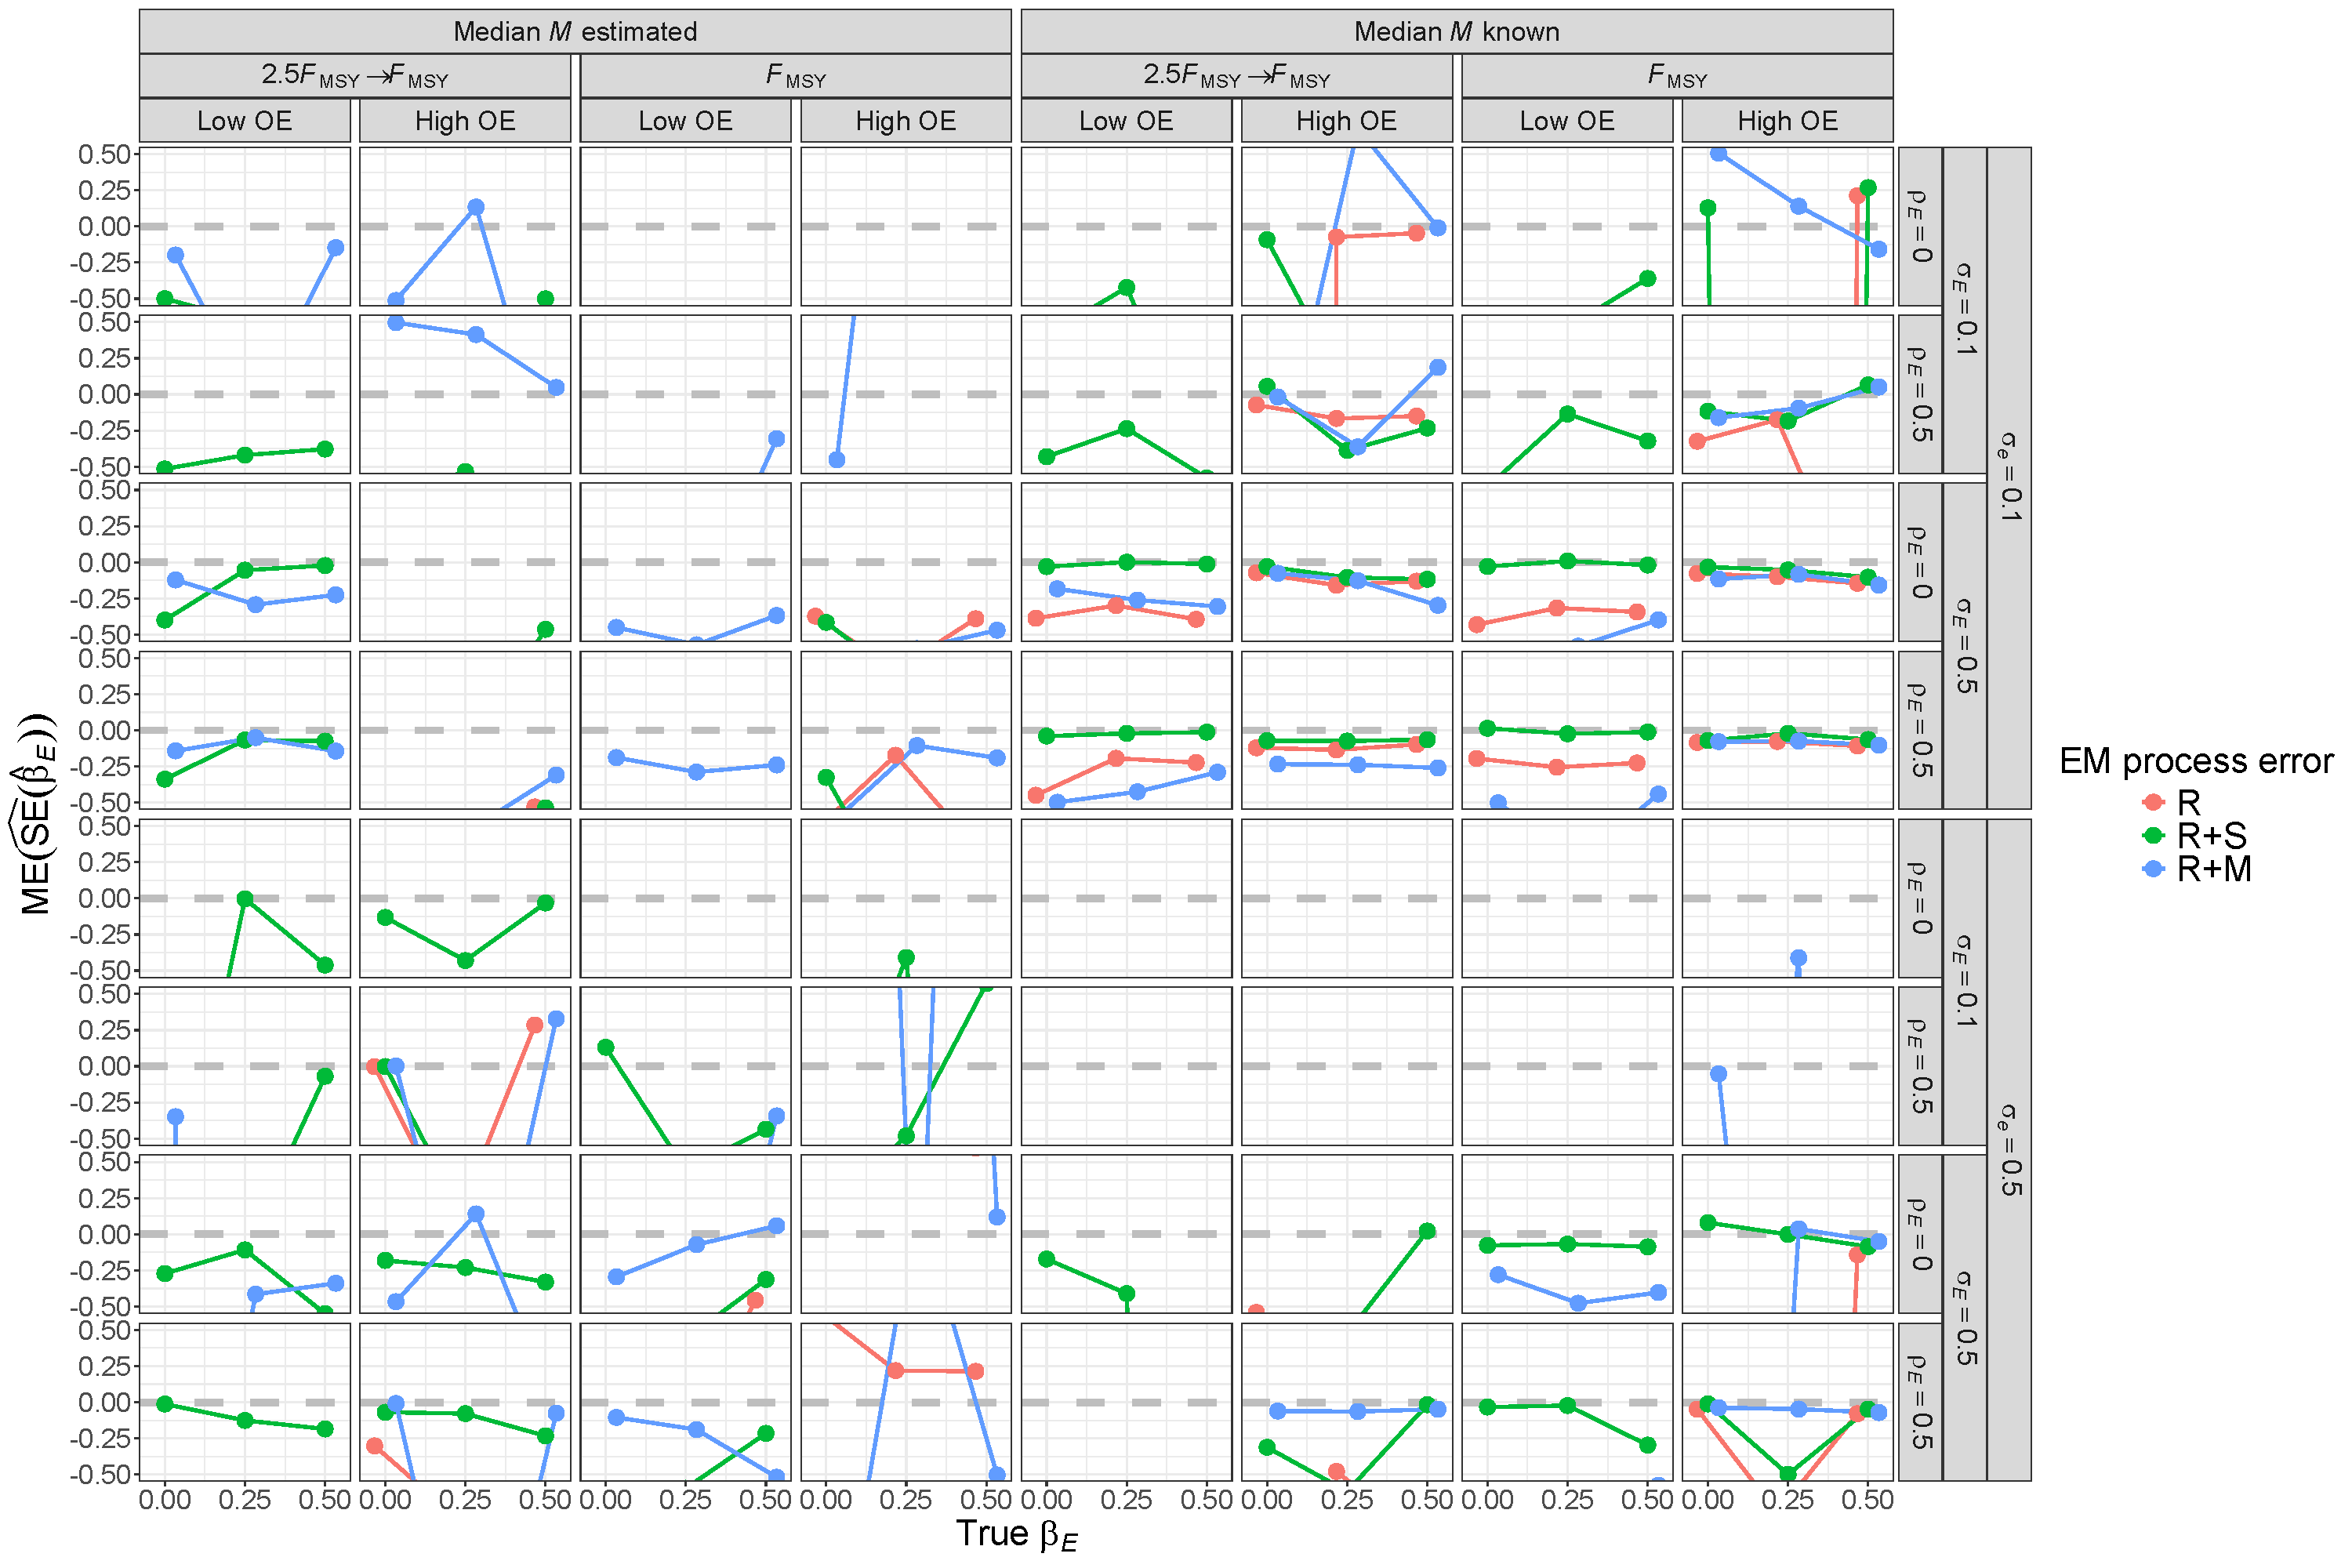
\includegraphics[height = \textheight]{se_beta_E_bias_RSom}
\end{center}
\caption{For R+S OMs, median error (ME) of Hessian-based estimates of standard error for covariate effect on \DIFdelbeginFL \DIFdelFL{natural mortality }\DIFdelendFL \DIFaddbeginFL \DIFaddFL{$M$ (}\DIFaddendFL $\beta_E$\DIFaddbeginFL \DIFaddFL{) }\DIFaddendFL from fitting EMs with alternative process error assumptions and treatment of median \DIFdelbeginFL \DIFdelFL{natural mortality }\DIFdelendFL \DIFaddbeginFL \DIFaddFL{$M$ }\DIFaddendFL ($e^\beta_M$ known or estimated). True standard error is defined as the mean of the standard error estimates accross converged fits to simulated data sets for a given OM scenario.}\label{se_beta_E_bias_RSom}
\end{figure}
\end{landscape}

\begin{landscape}
\begin{figure}
\begin{center}
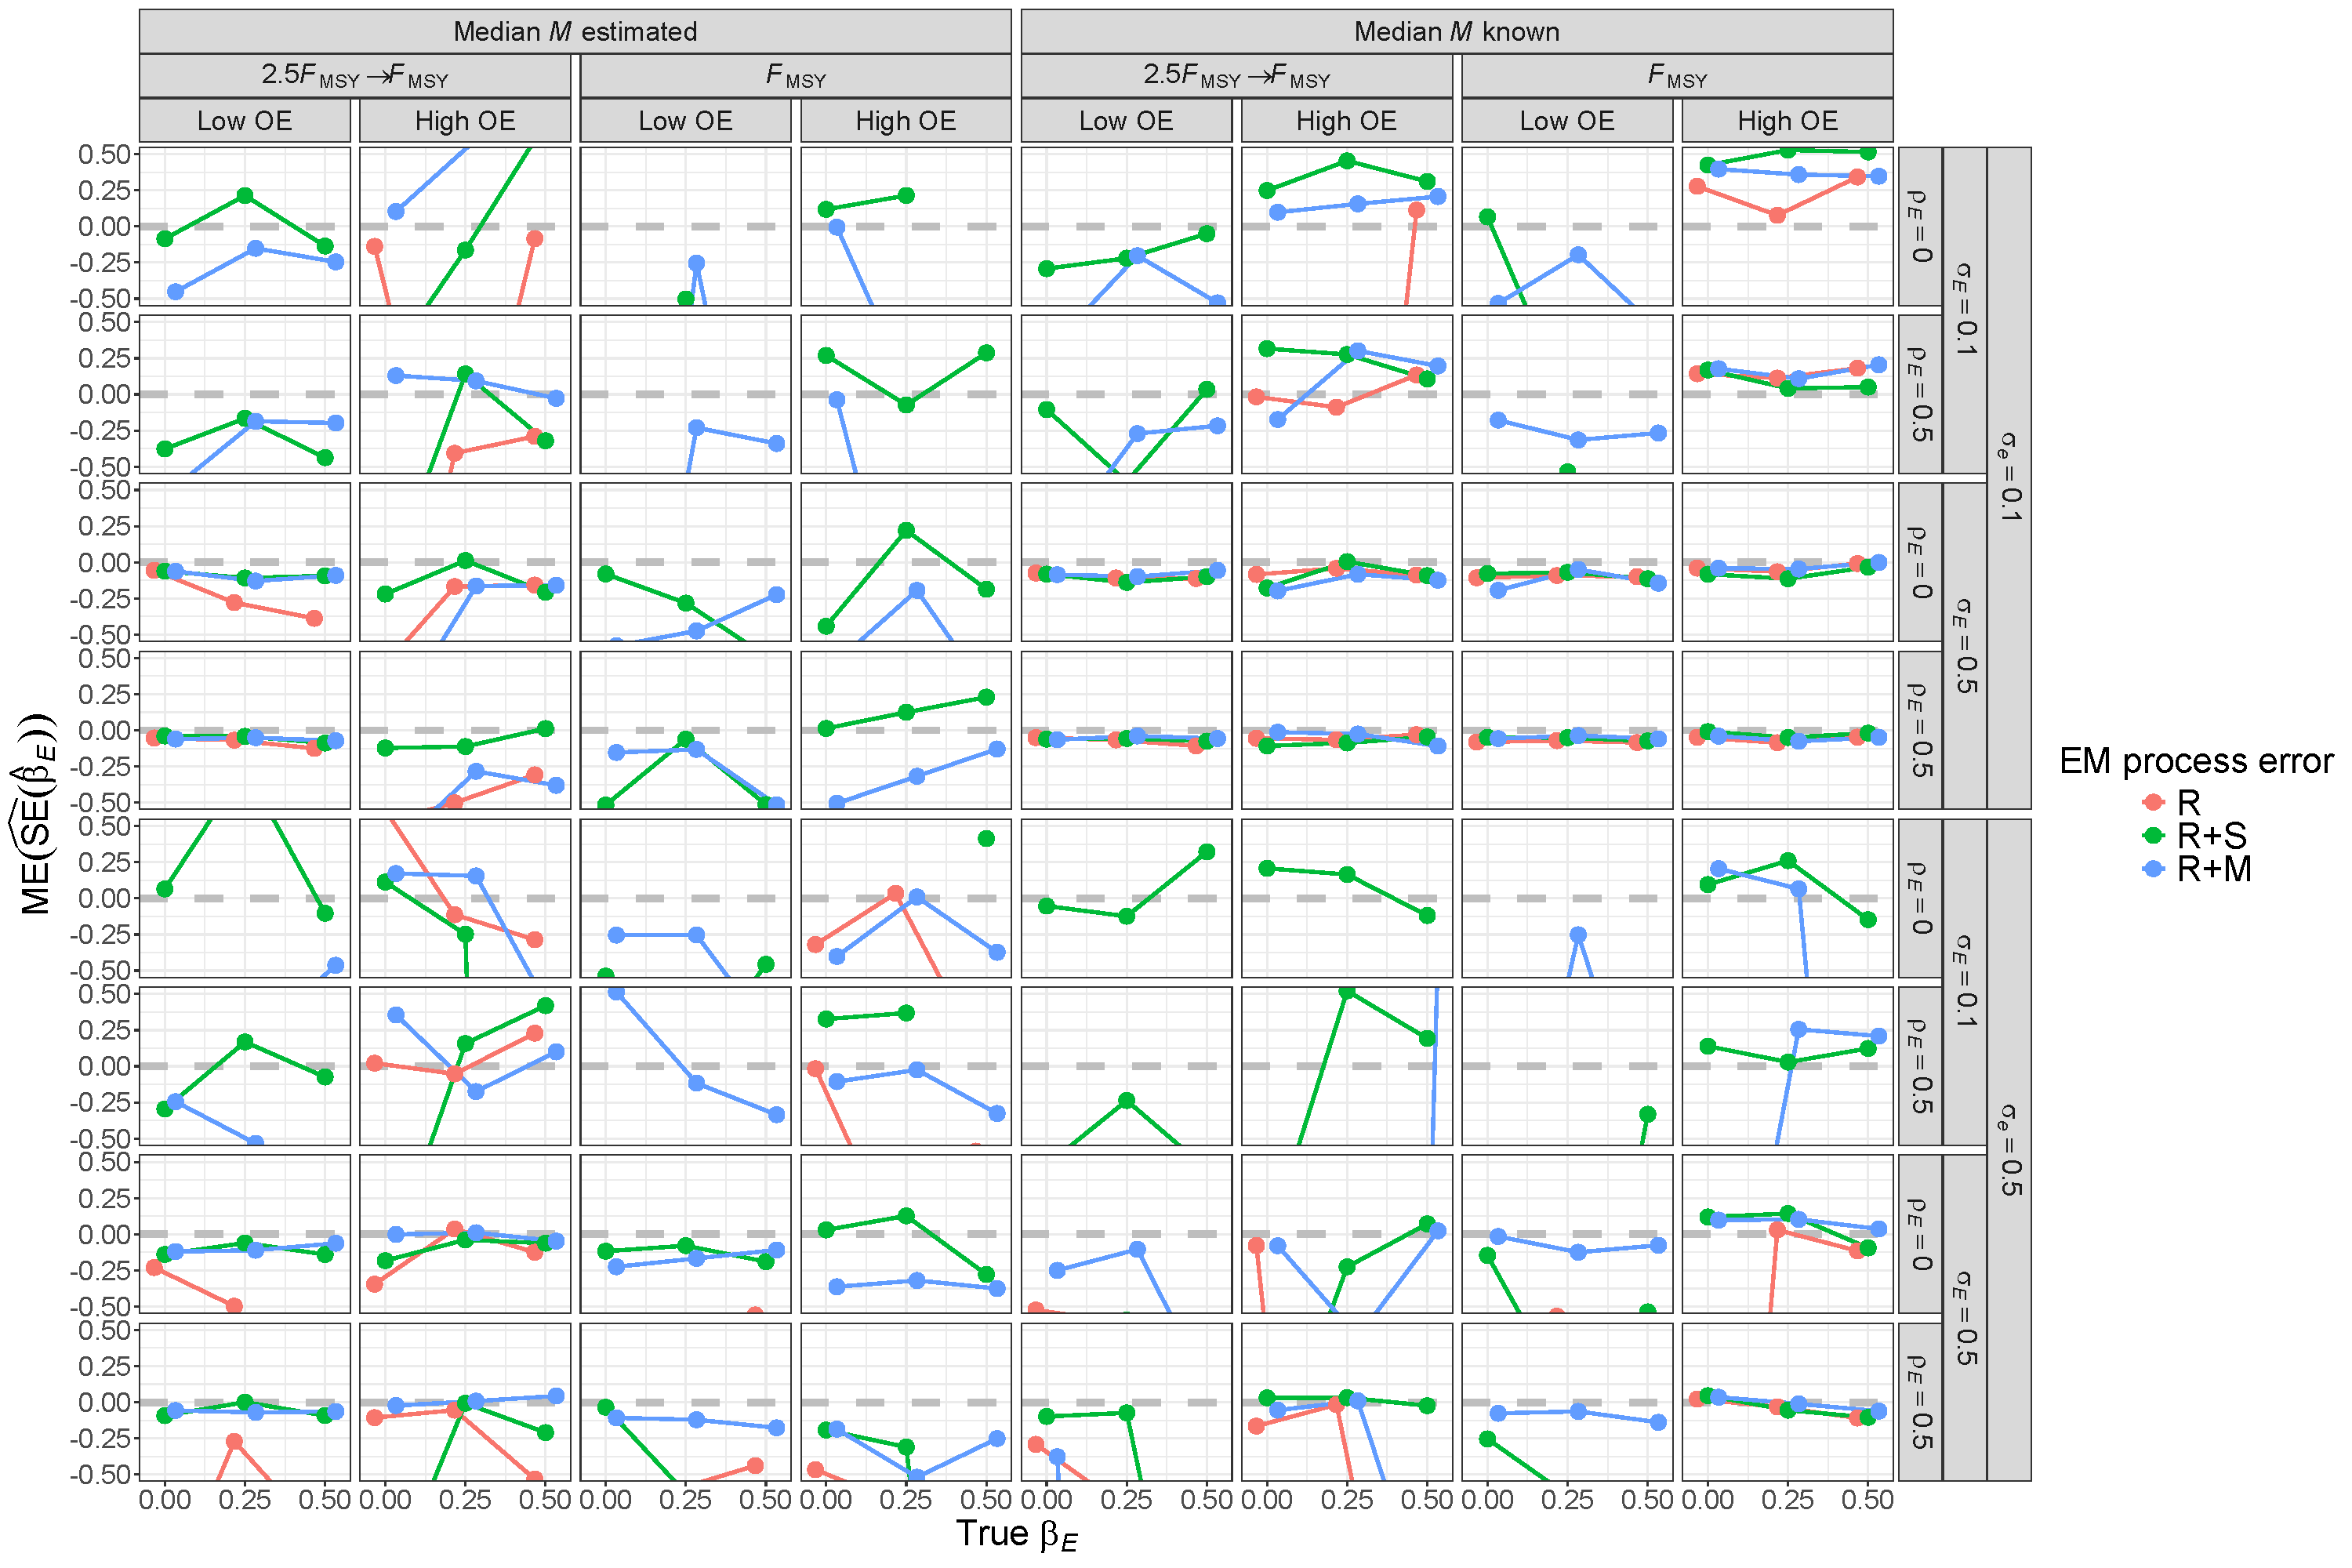
\includegraphics[height = \textheight]{se_beta_E_bias_RMom}
\end{center}
\caption{For R+M OMs, median error (ME) of Hessian-based estimates of standard error for covariate effect on \DIFdelbeginFL \DIFdelFL{natural mortality }\DIFdelendFL \DIFaddbeginFL \DIFaddFL{$M$ (}\DIFaddendFL $\beta_E$\DIFaddbeginFL \DIFaddFL{) }\DIFaddendFL from fitting EMs with alternative process error assumptions and treatment of median \DIFdelbeginFL \DIFdelFL{natural mortality }\DIFdelendFL \DIFaddbeginFL \DIFaddFL{$M$ }\DIFaddendFL ($e^\beta_M$ known or estimated). True standard error is defined as the mean of the standard error estimates accross converged fits to simulated data sets for a given OM scenario.}\label{se_beta_E_bias_RMom}
\end{figure}
\end{landscape}

\DIFdelbegin %DIFDELCMD < \hypertarget{covariate-effect-confidence-interval-coverage}{%
%DIFDELCMD < \subsection*{Covariate effect confidence interval coverage}\label{covariate-effect-confidence-interval-coverage}}
%DIFDELCMD < %%%
\DIFdelend \DIFaddbegin \subsection*{\DIFadd{Covariate effect confidence interval coverage}}\label{covariate-effect-confidence-interval-coverage}
\DIFaddend \addcontentsline{toc}{subsection}{Covariate effect confidence interval coverage}

\begin{landscape}
\begin{figure}
\begin{center}
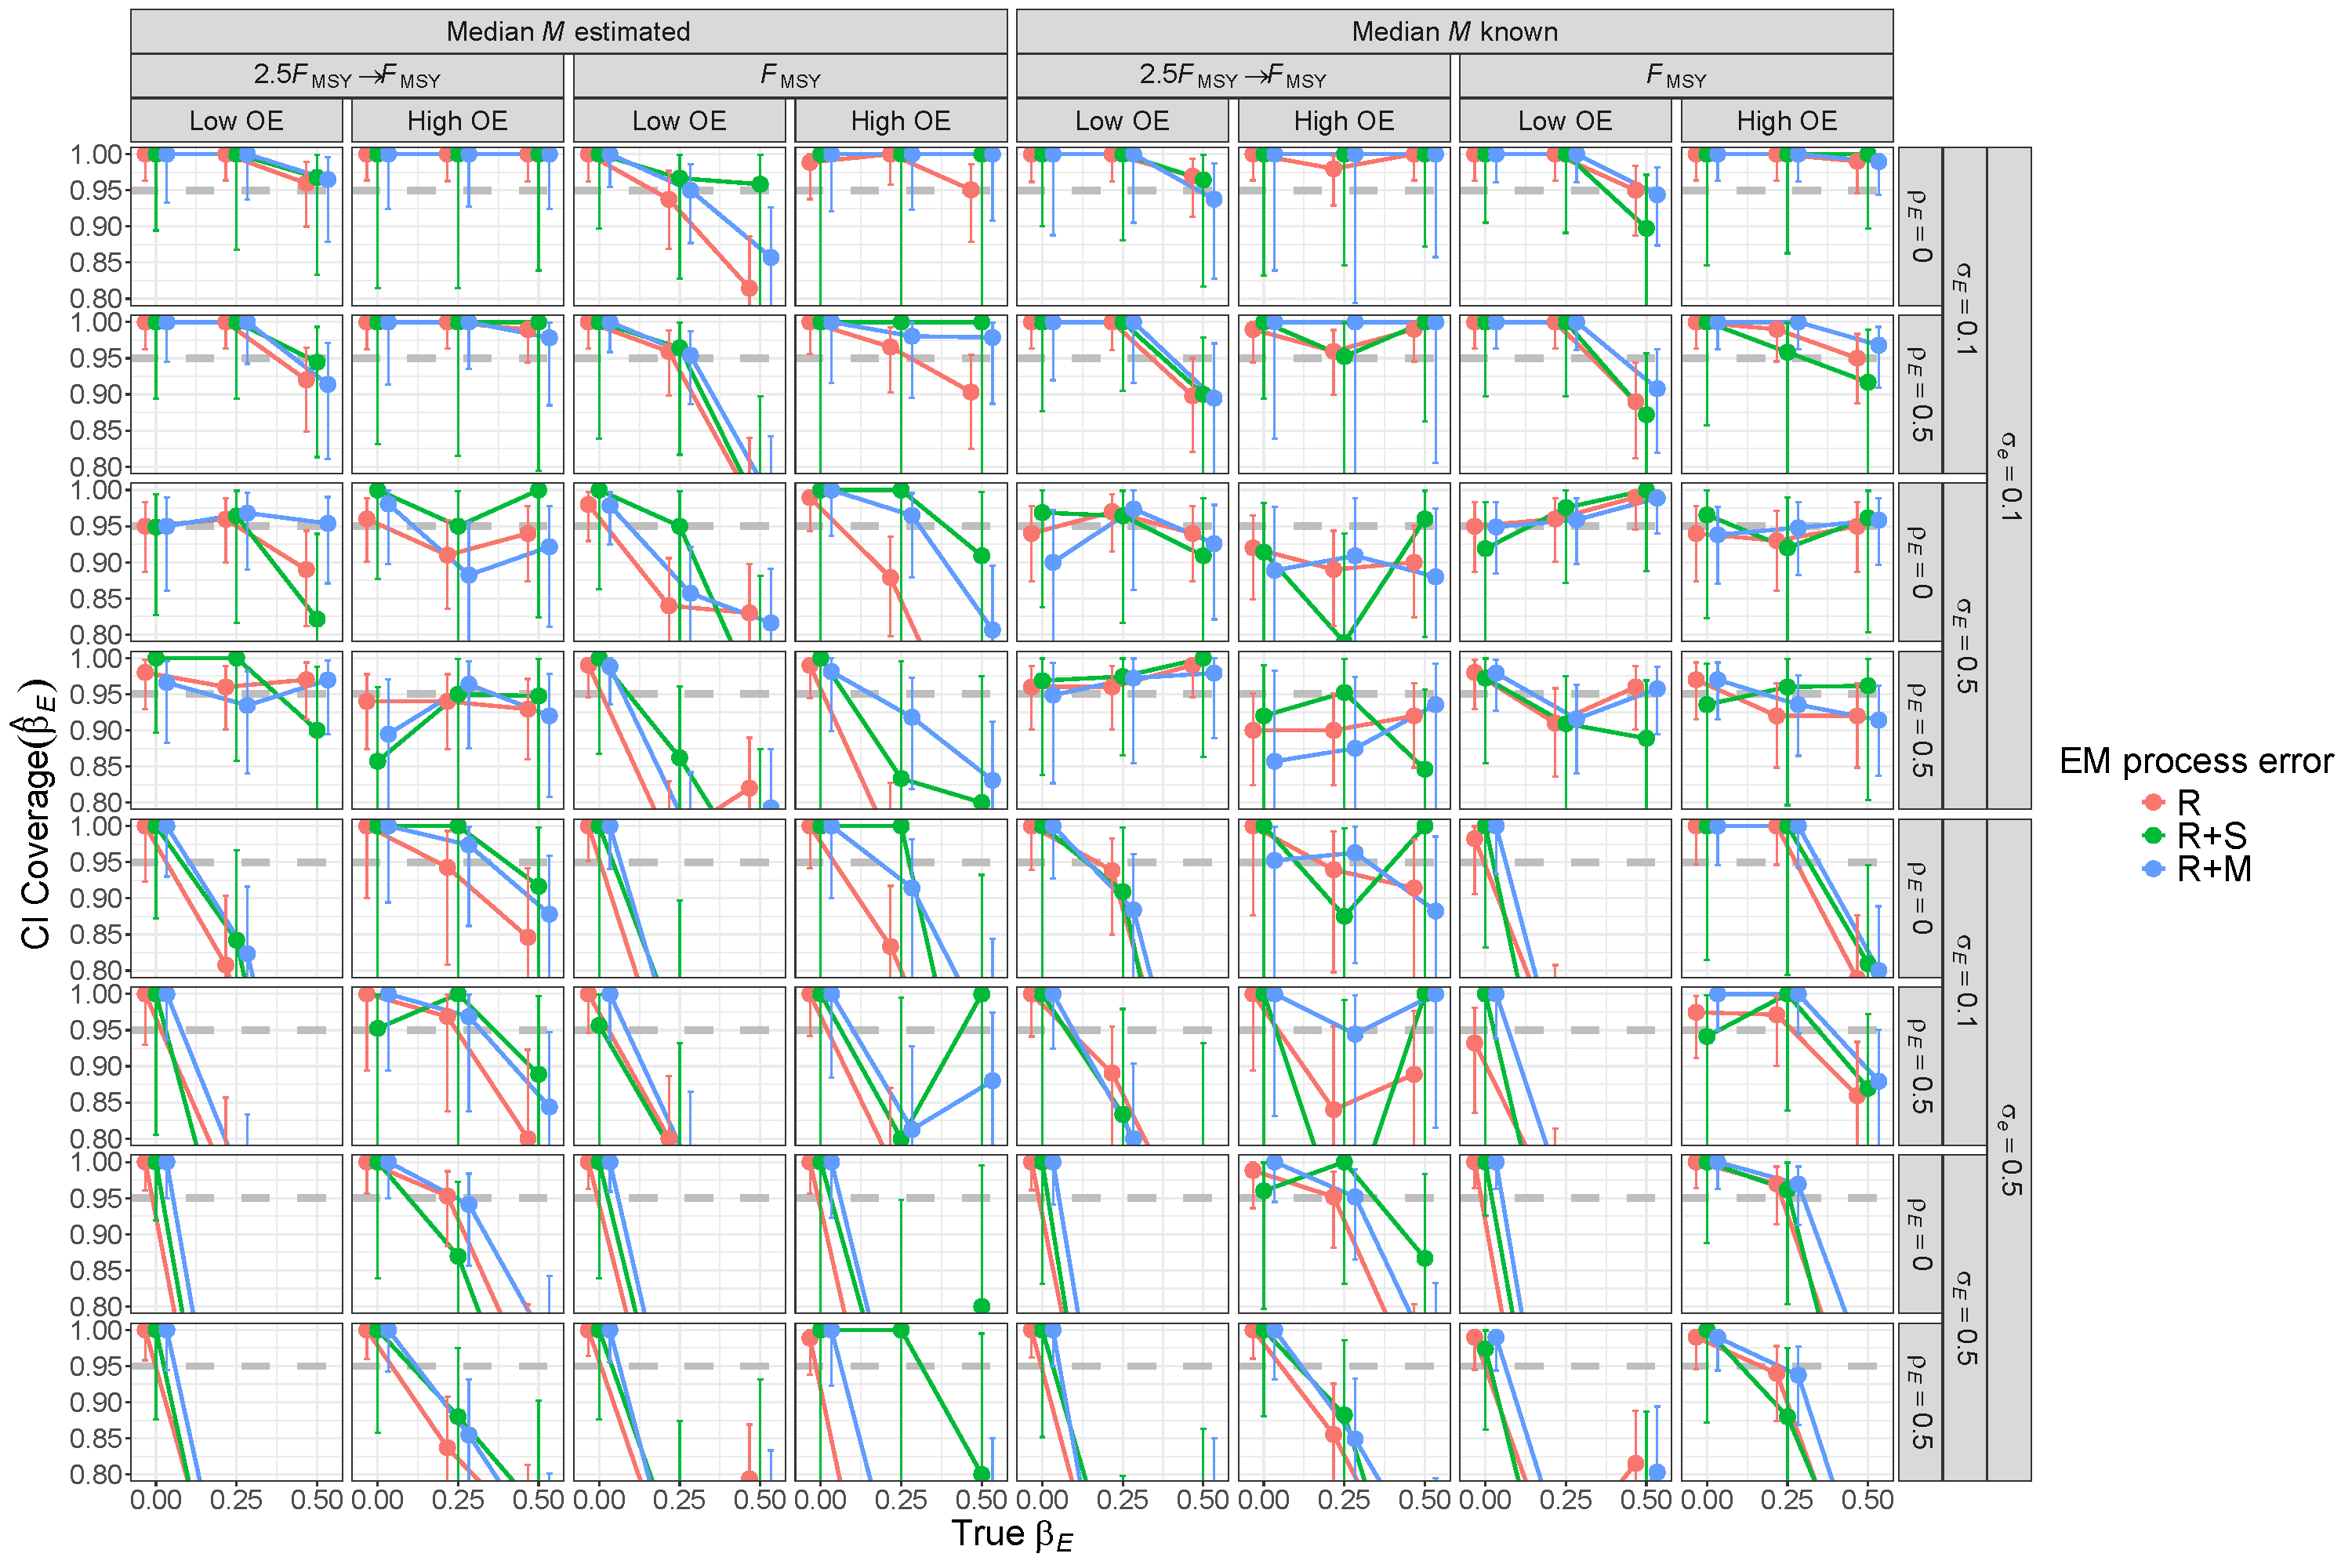
\includegraphics[height = \textheight]{beta_E_CI_coverage_Rom}
\end{center}
\caption{For R OMs, probability of 95\% confidence interval for $\beta_E$ containing the true value for EMs with alternative process error assumptions and treatment of median \DIFdelbeginFL \DIFdelFL{natural mortality }\DIFdelendFL \DIFaddbeginFL \DIFaddFL{$M$ }\DIFaddendFL ($e^\beta_M$ known or estimated). Vertical lines represent 95\% confidence intervals.}\label{beta_E_CI_coverage_Rom}
\end{figure}
\end{landscape}

\begin{landscape}
\begin{figure}
\begin{center}
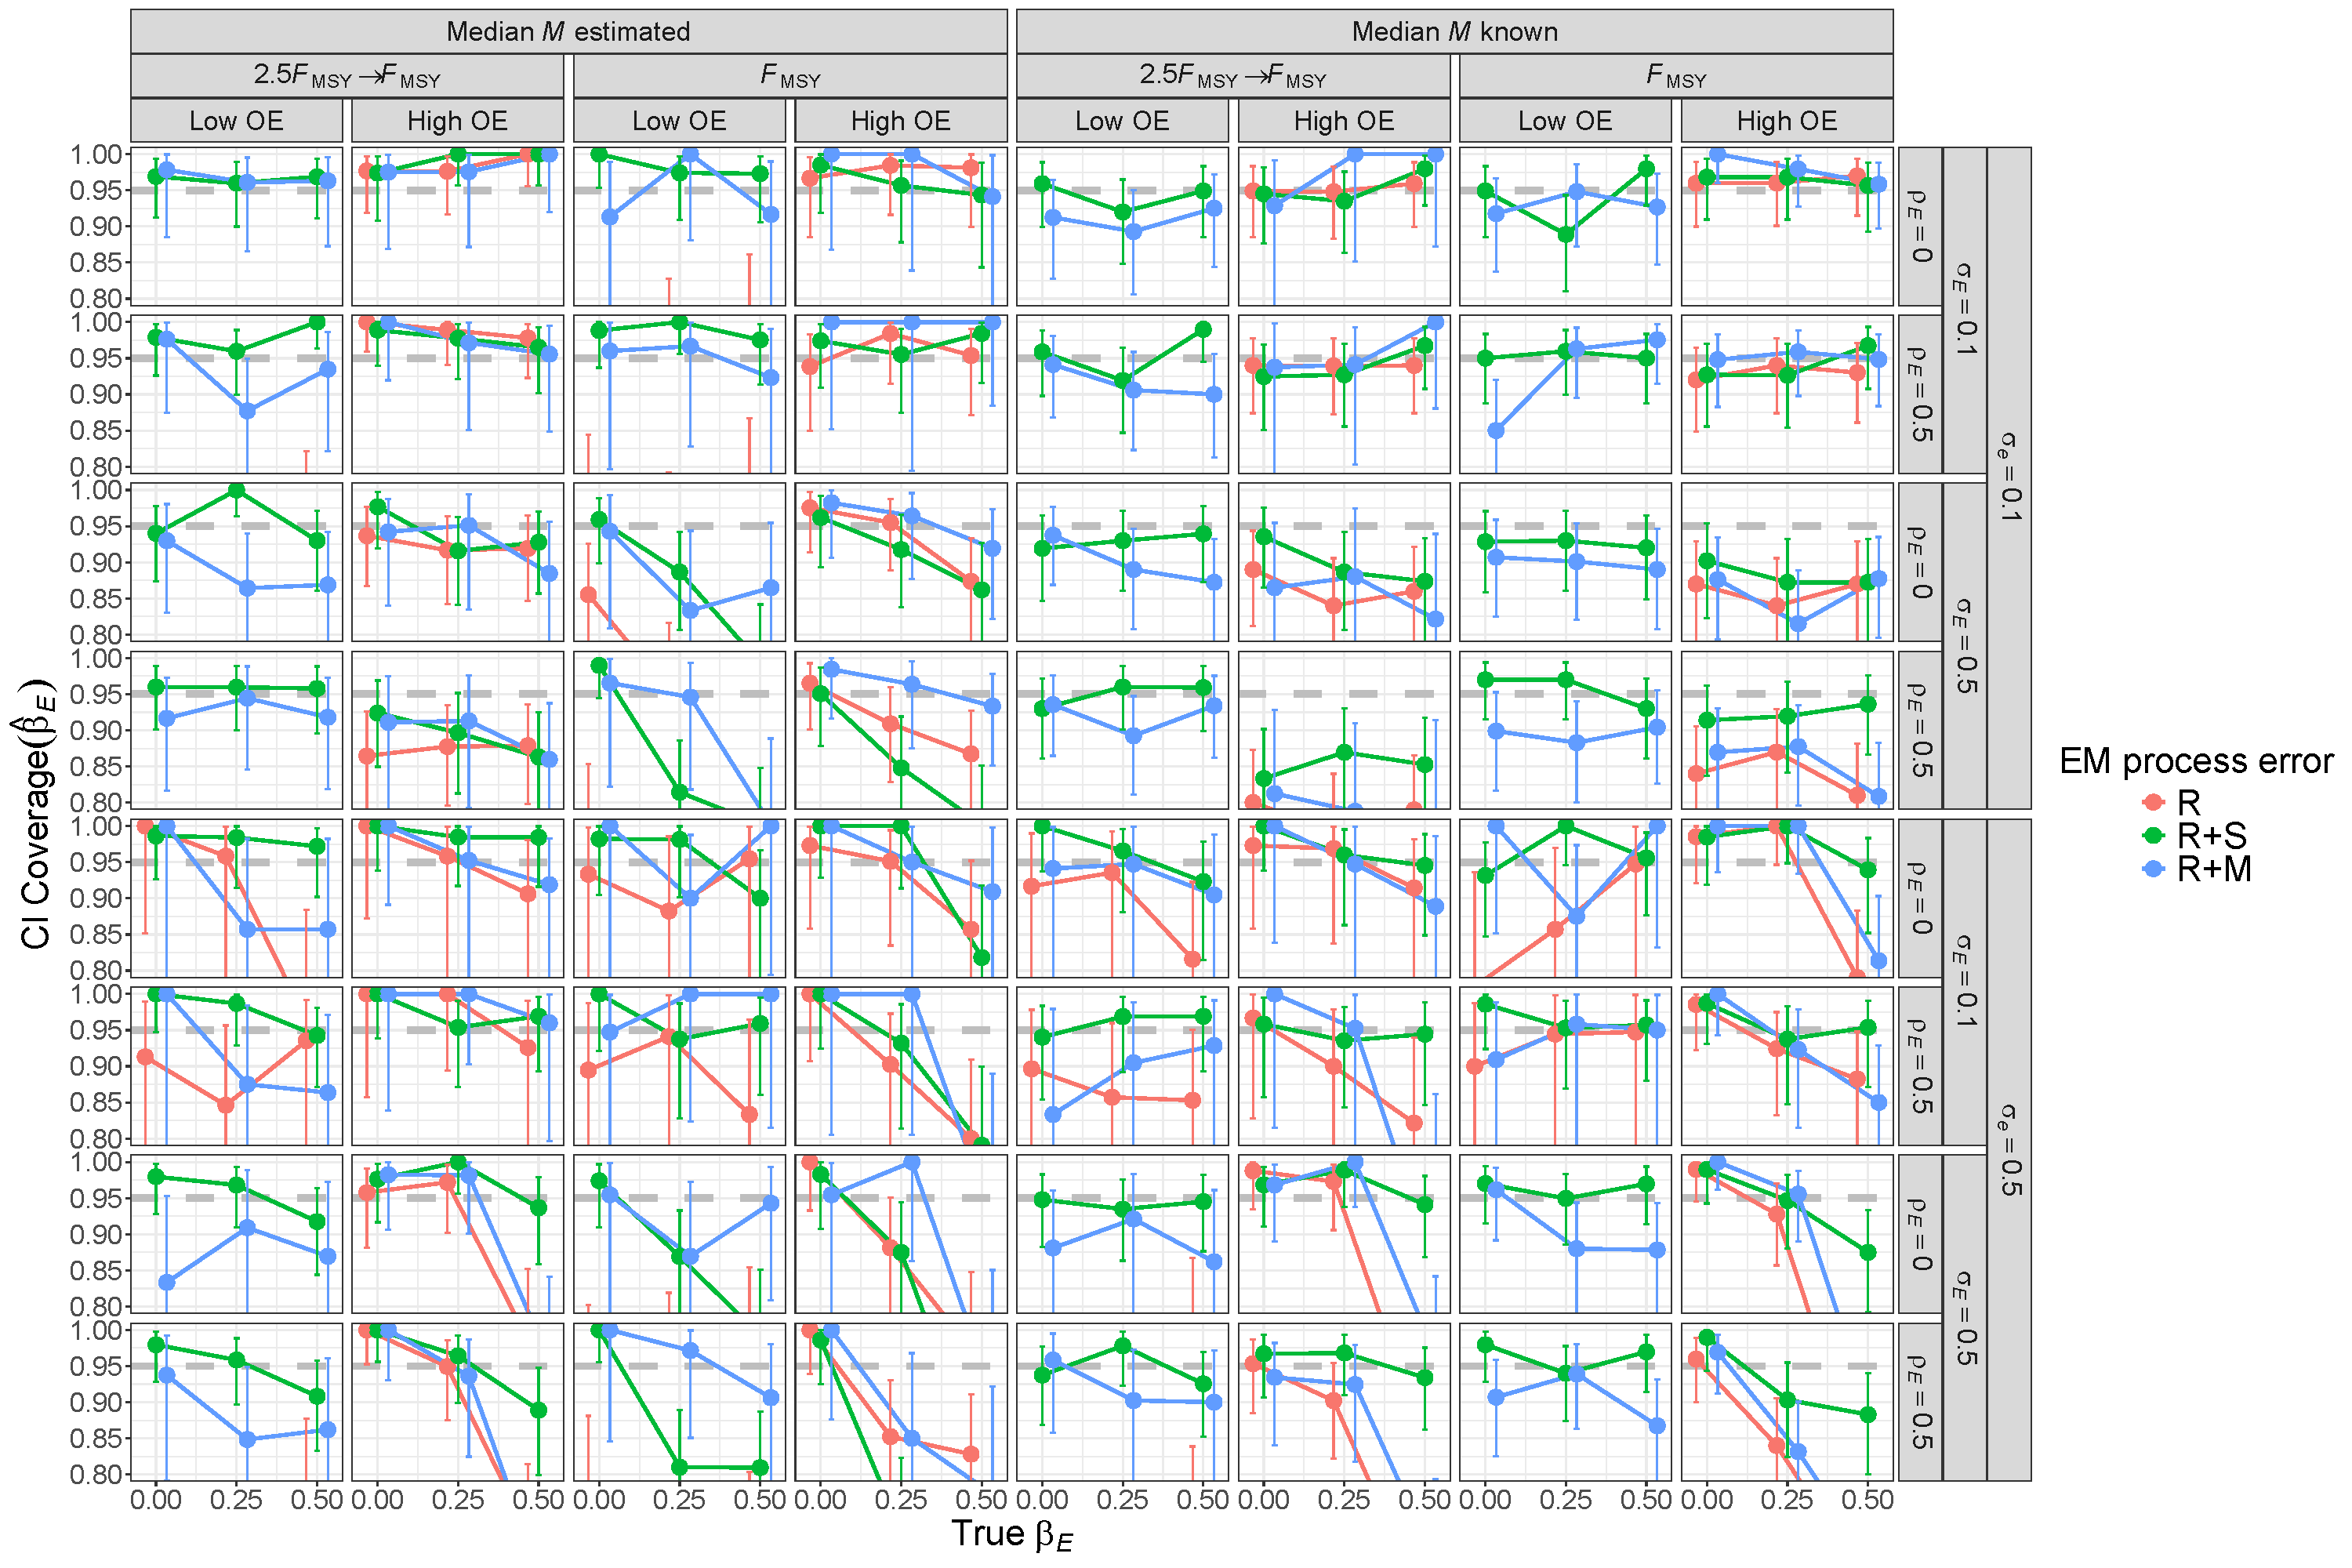
\includegraphics[height = \textheight]{beta_E_CI_coverage_RSom}
\end{center}
\caption{For R+S OMs, probability of 95\% confidence interval for $\beta_E$ containing the true value for EMs with alternative process error assumptions and treatment of median \DIFdelbeginFL \DIFdelFL{natural mortality }\DIFdelendFL \DIFaddbeginFL \DIFaddFL{$M$ }\DIFaddendFL ($e^\beta_M$ known or estimated). Vertical lines represent 95\% confidence intervals.}\label{beta_E_CI_coverage_RSom}
\end{figure}
\end{landscape}

\begin{landscape}
\begin{figure}
\begin{center}
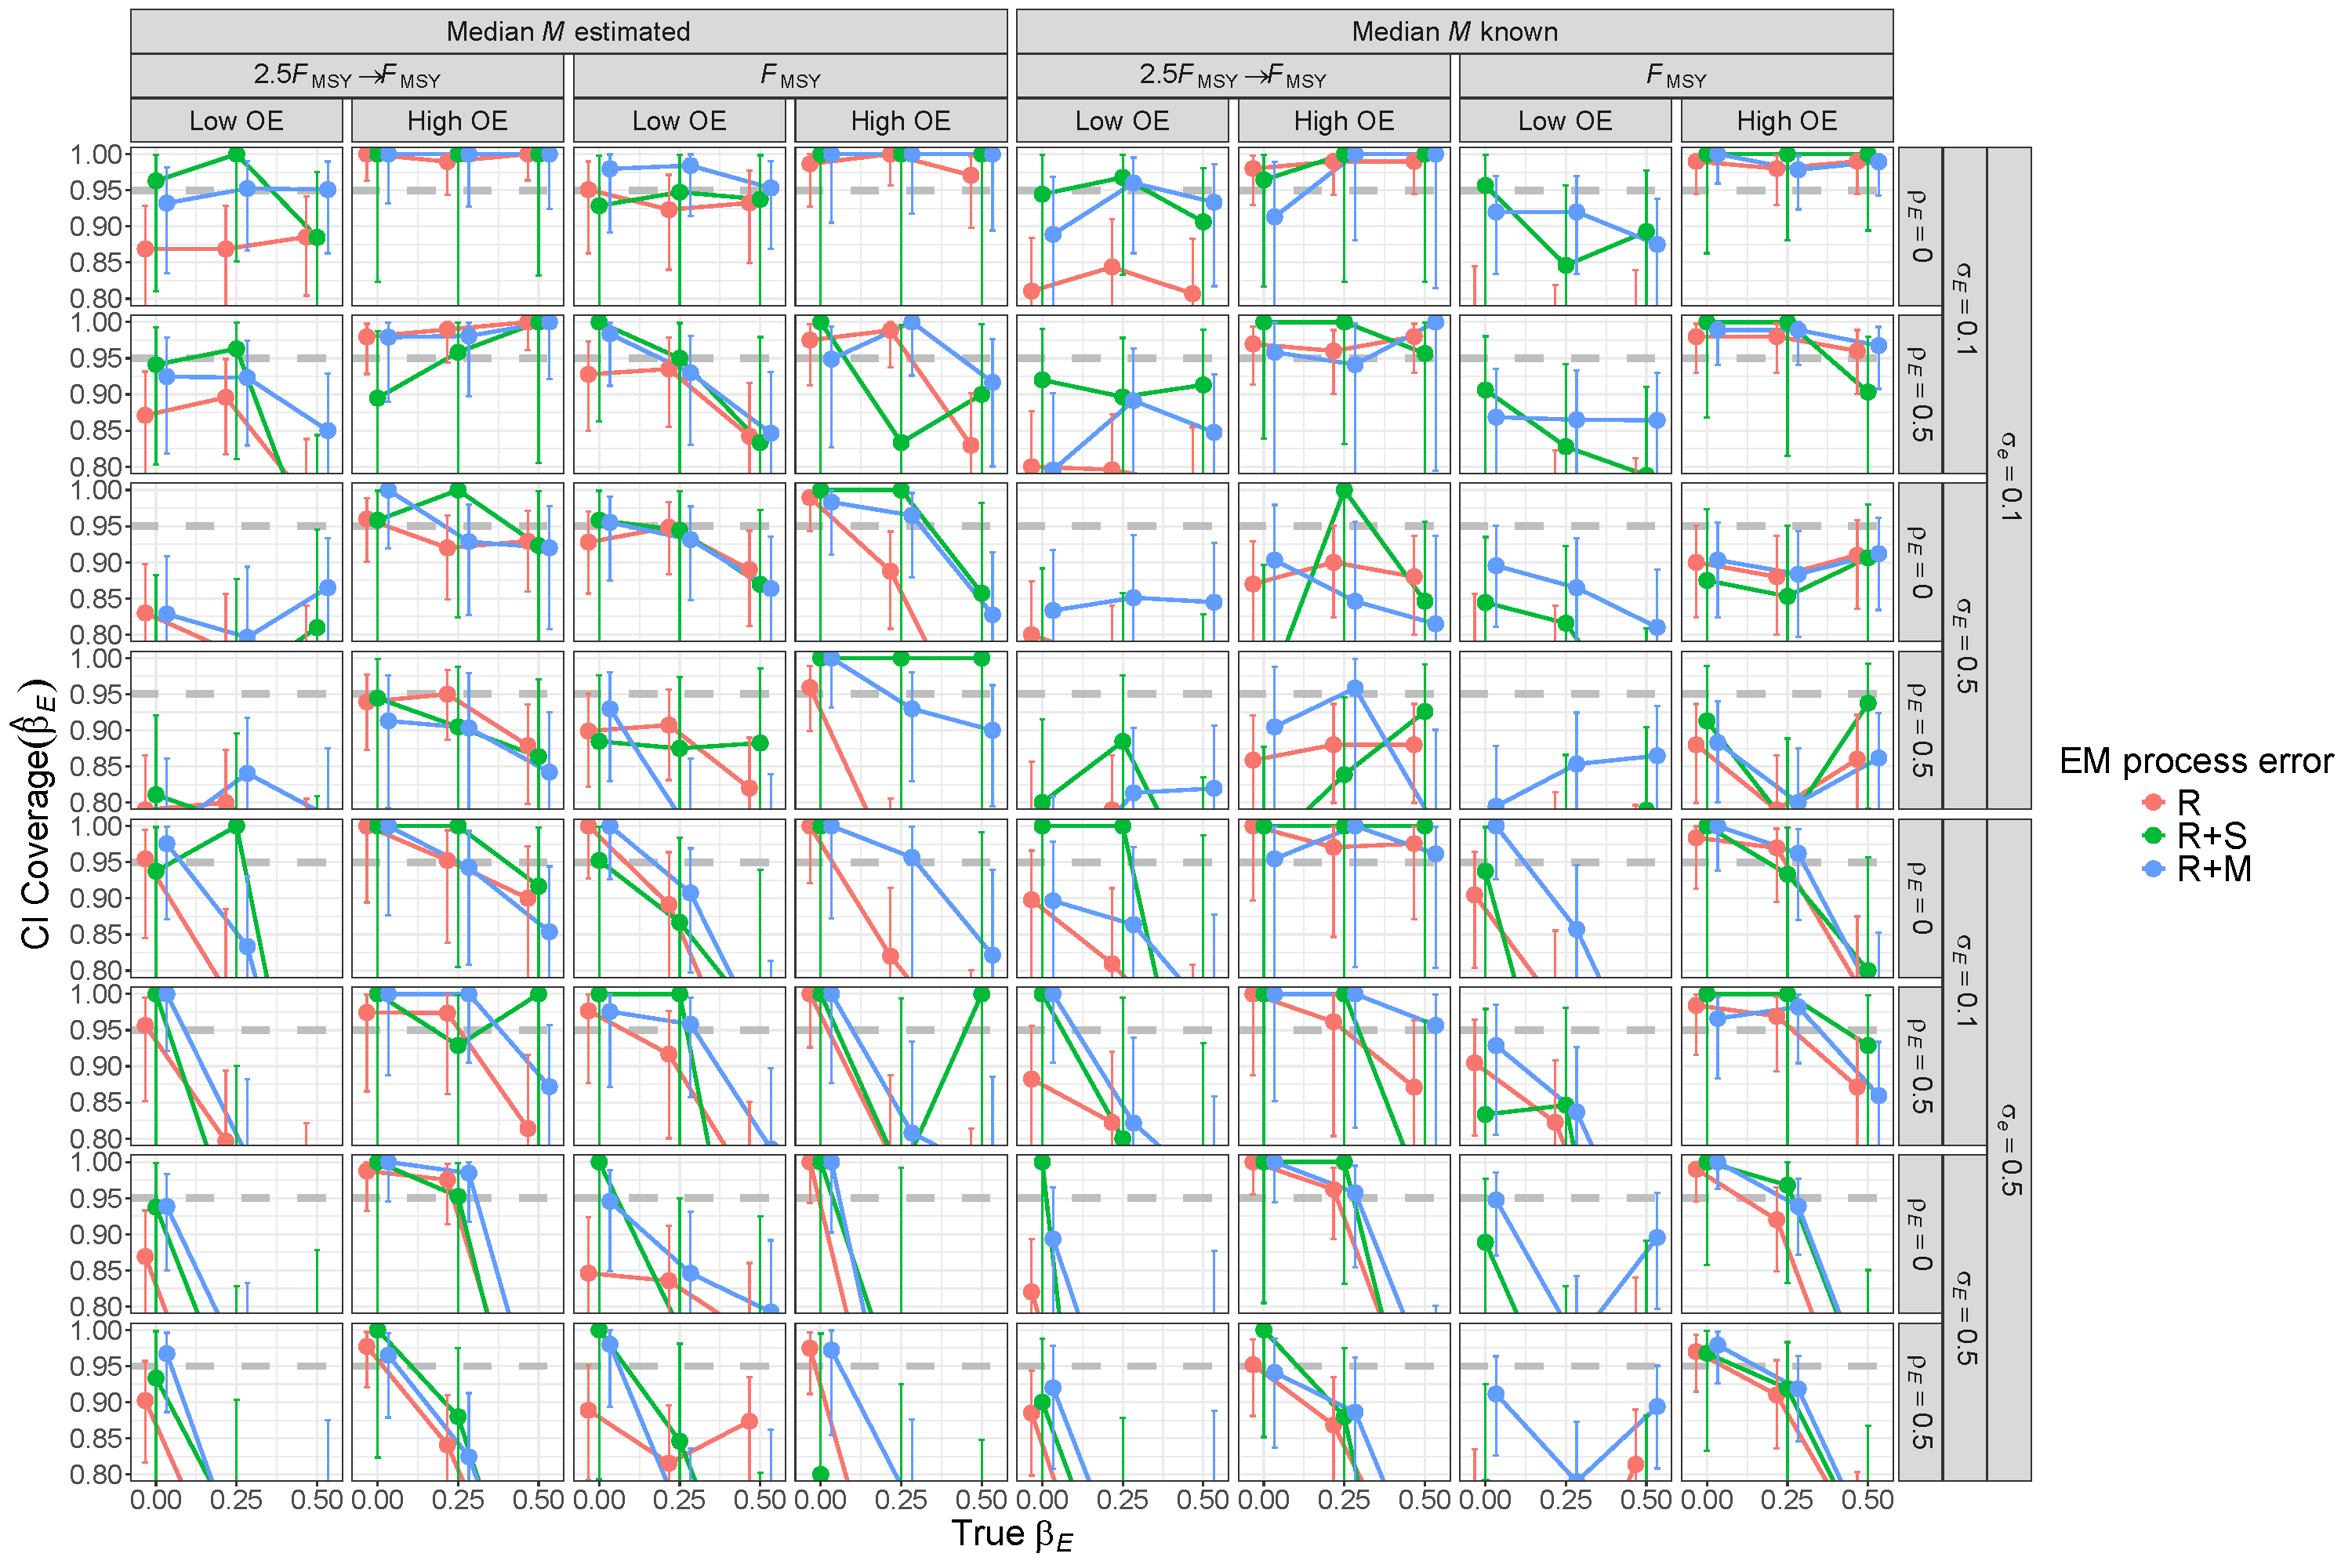
\includegraphics[height = \textheight]{beta_E_CI_coverage_RMom}
\end{center}
\caption{For R+M OMs, probability of 95\% confidence interval for $\beta_E$ containing the true value for EMs with alternative process error assumptions and treatment of median \DIFdelbeginFL \DIFdelFL{natural mortality }\DIFdelendFL \DIFaddbeginFL \DIFaddFL{$M$ }\DIFaddendFL ($e^\beta_M$ known or estimated). Vertical lines represent 95\% confidence intervals.}\label{beta_E_CI_coverage_RMom}
\end{figure}
\end{landscape}

\DIFdelbegin %DIFDELCMD < \hypertarget{covariate-effect-rmse}{%
%DIFDELCMD < \subsection*{Covariate effect RMSE}\label{covariate-effect-rmse}}
%DIFDELCMD < %%%
\DIFdelend \DIFaddbegin \subsection*{\DIFadd{Covariate effect RMSE}}\label{covariate-effect-rmse}
\DIFaddend \addcontentsline{toc}{subsection}{Covariate effect RMSE}

\begin{landscape}
\begin{figure}
\begin{center}
\DIFdelbeginFL %DIFDELCMD < 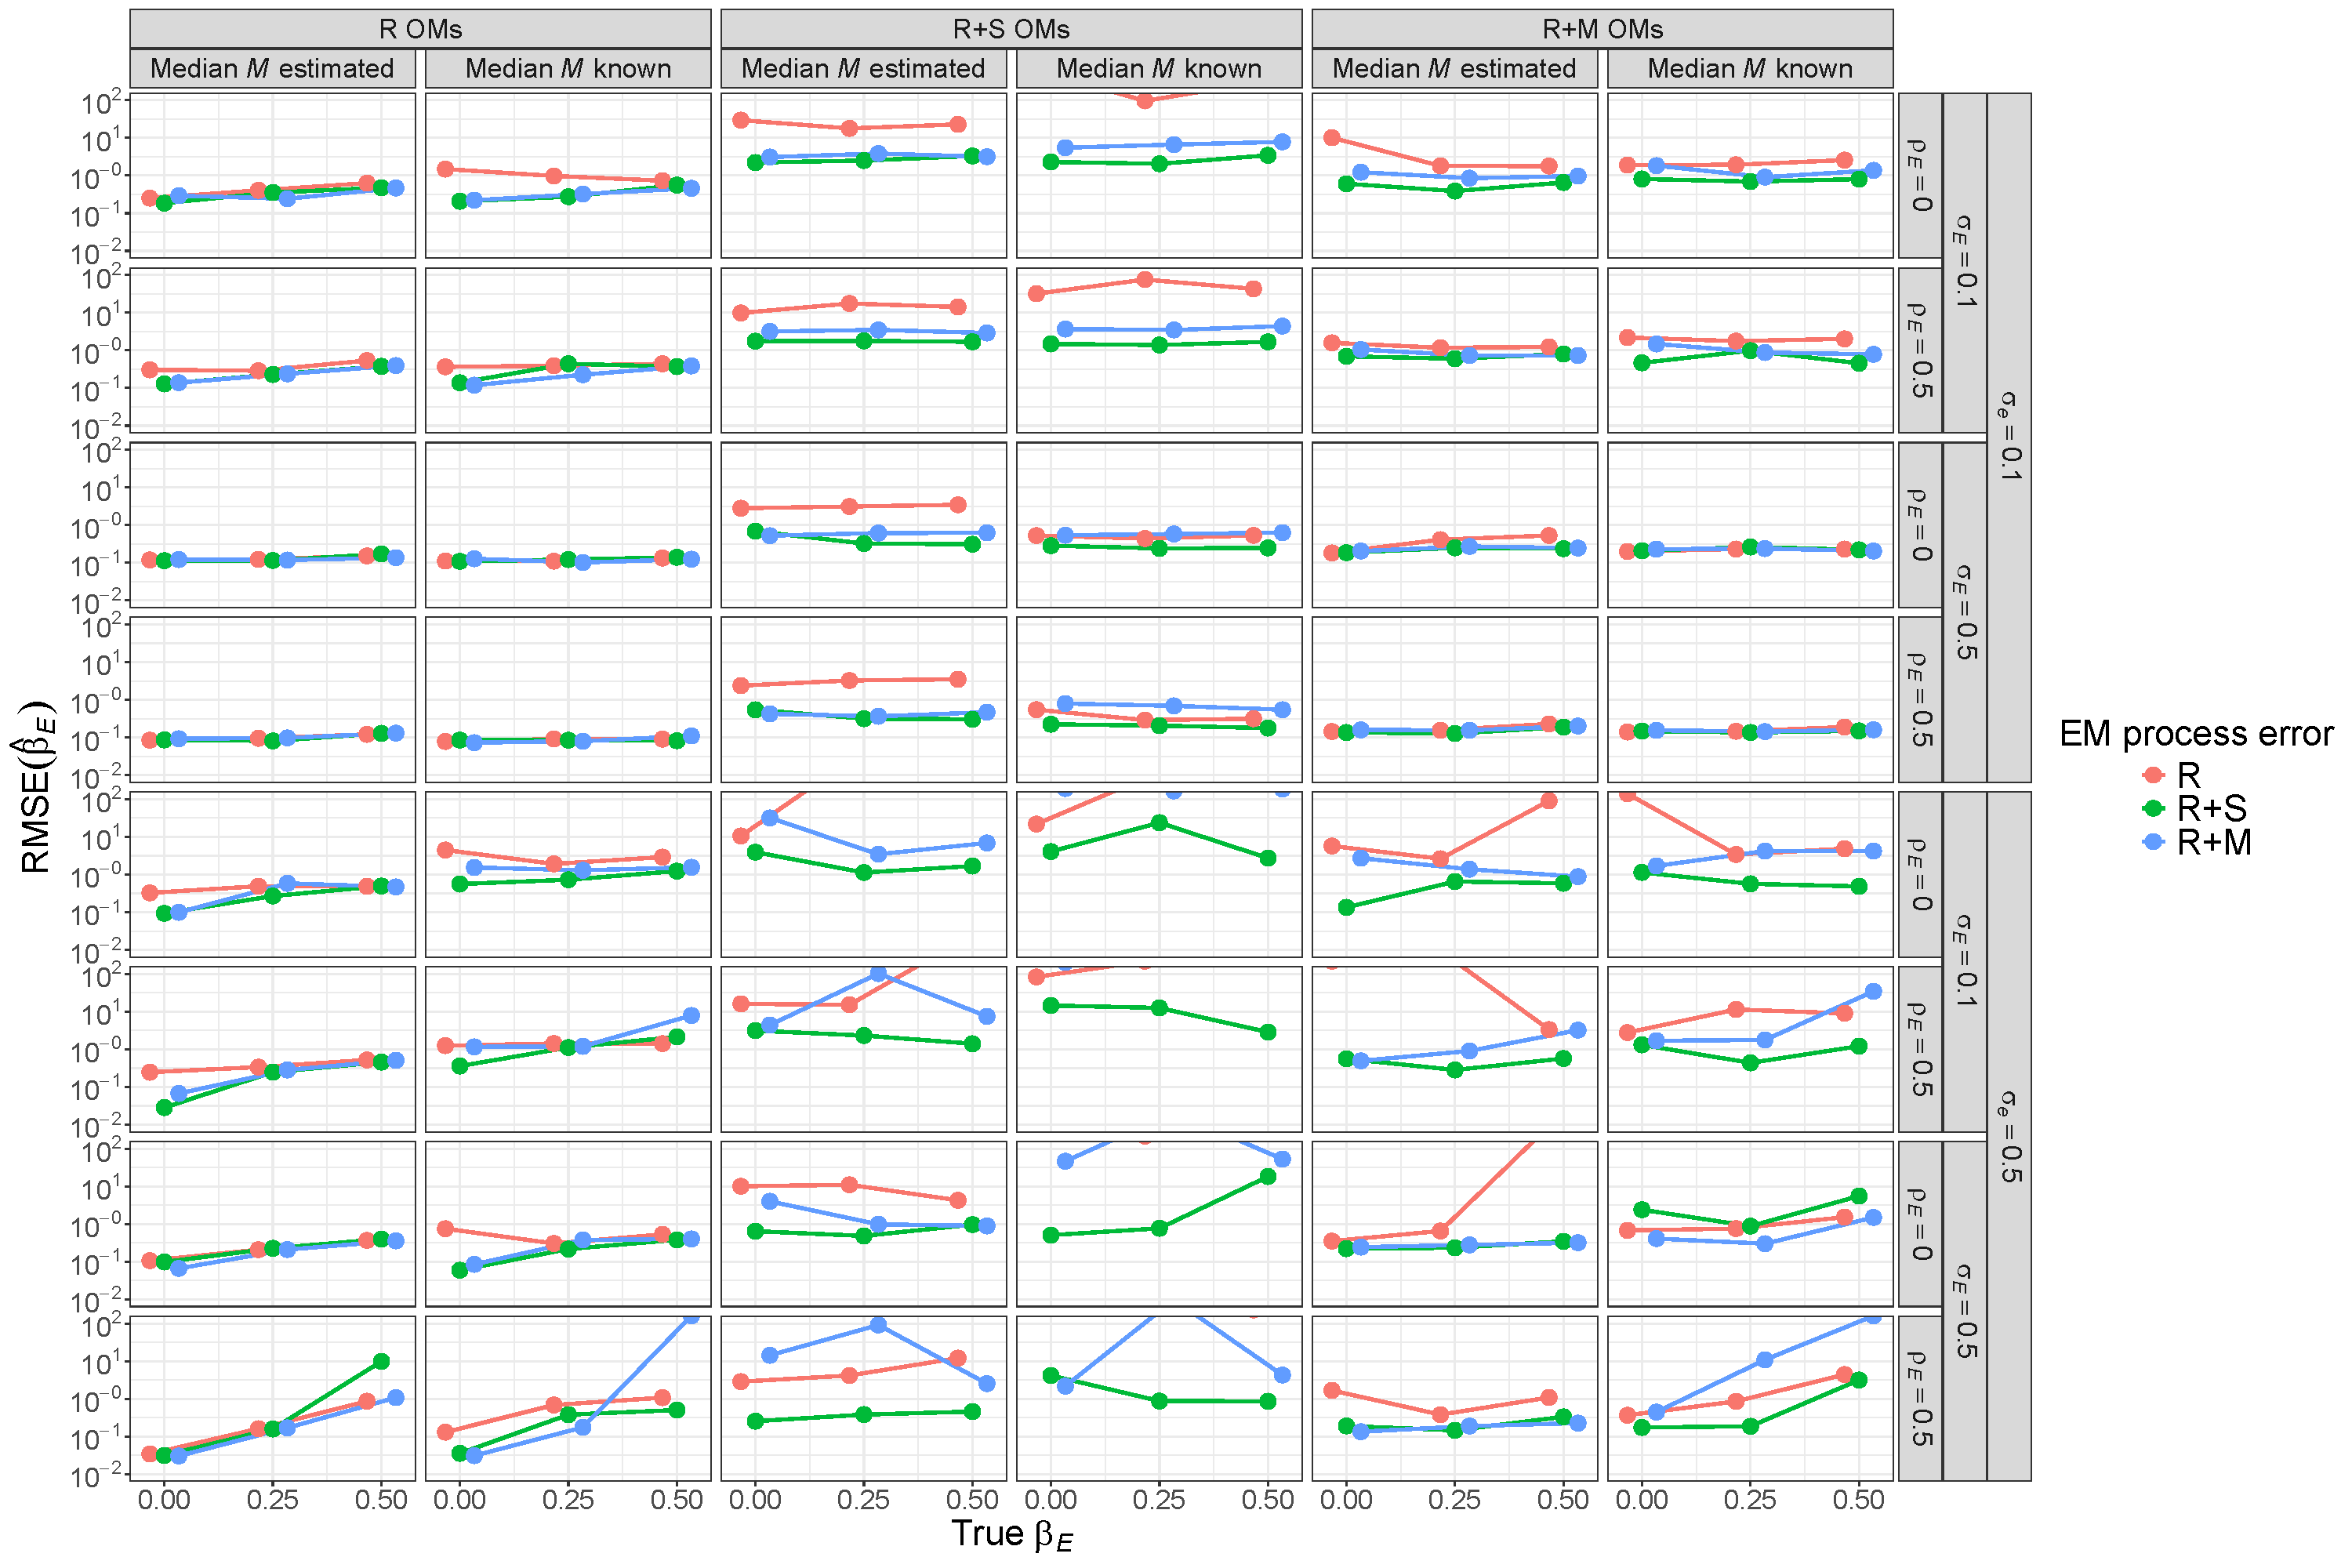
\includegraphics[height = \textheight]{beta_E_rmse_main}
%DIFDELCMD < %%%
\DIFdelendFL \DIFaddbeginFL 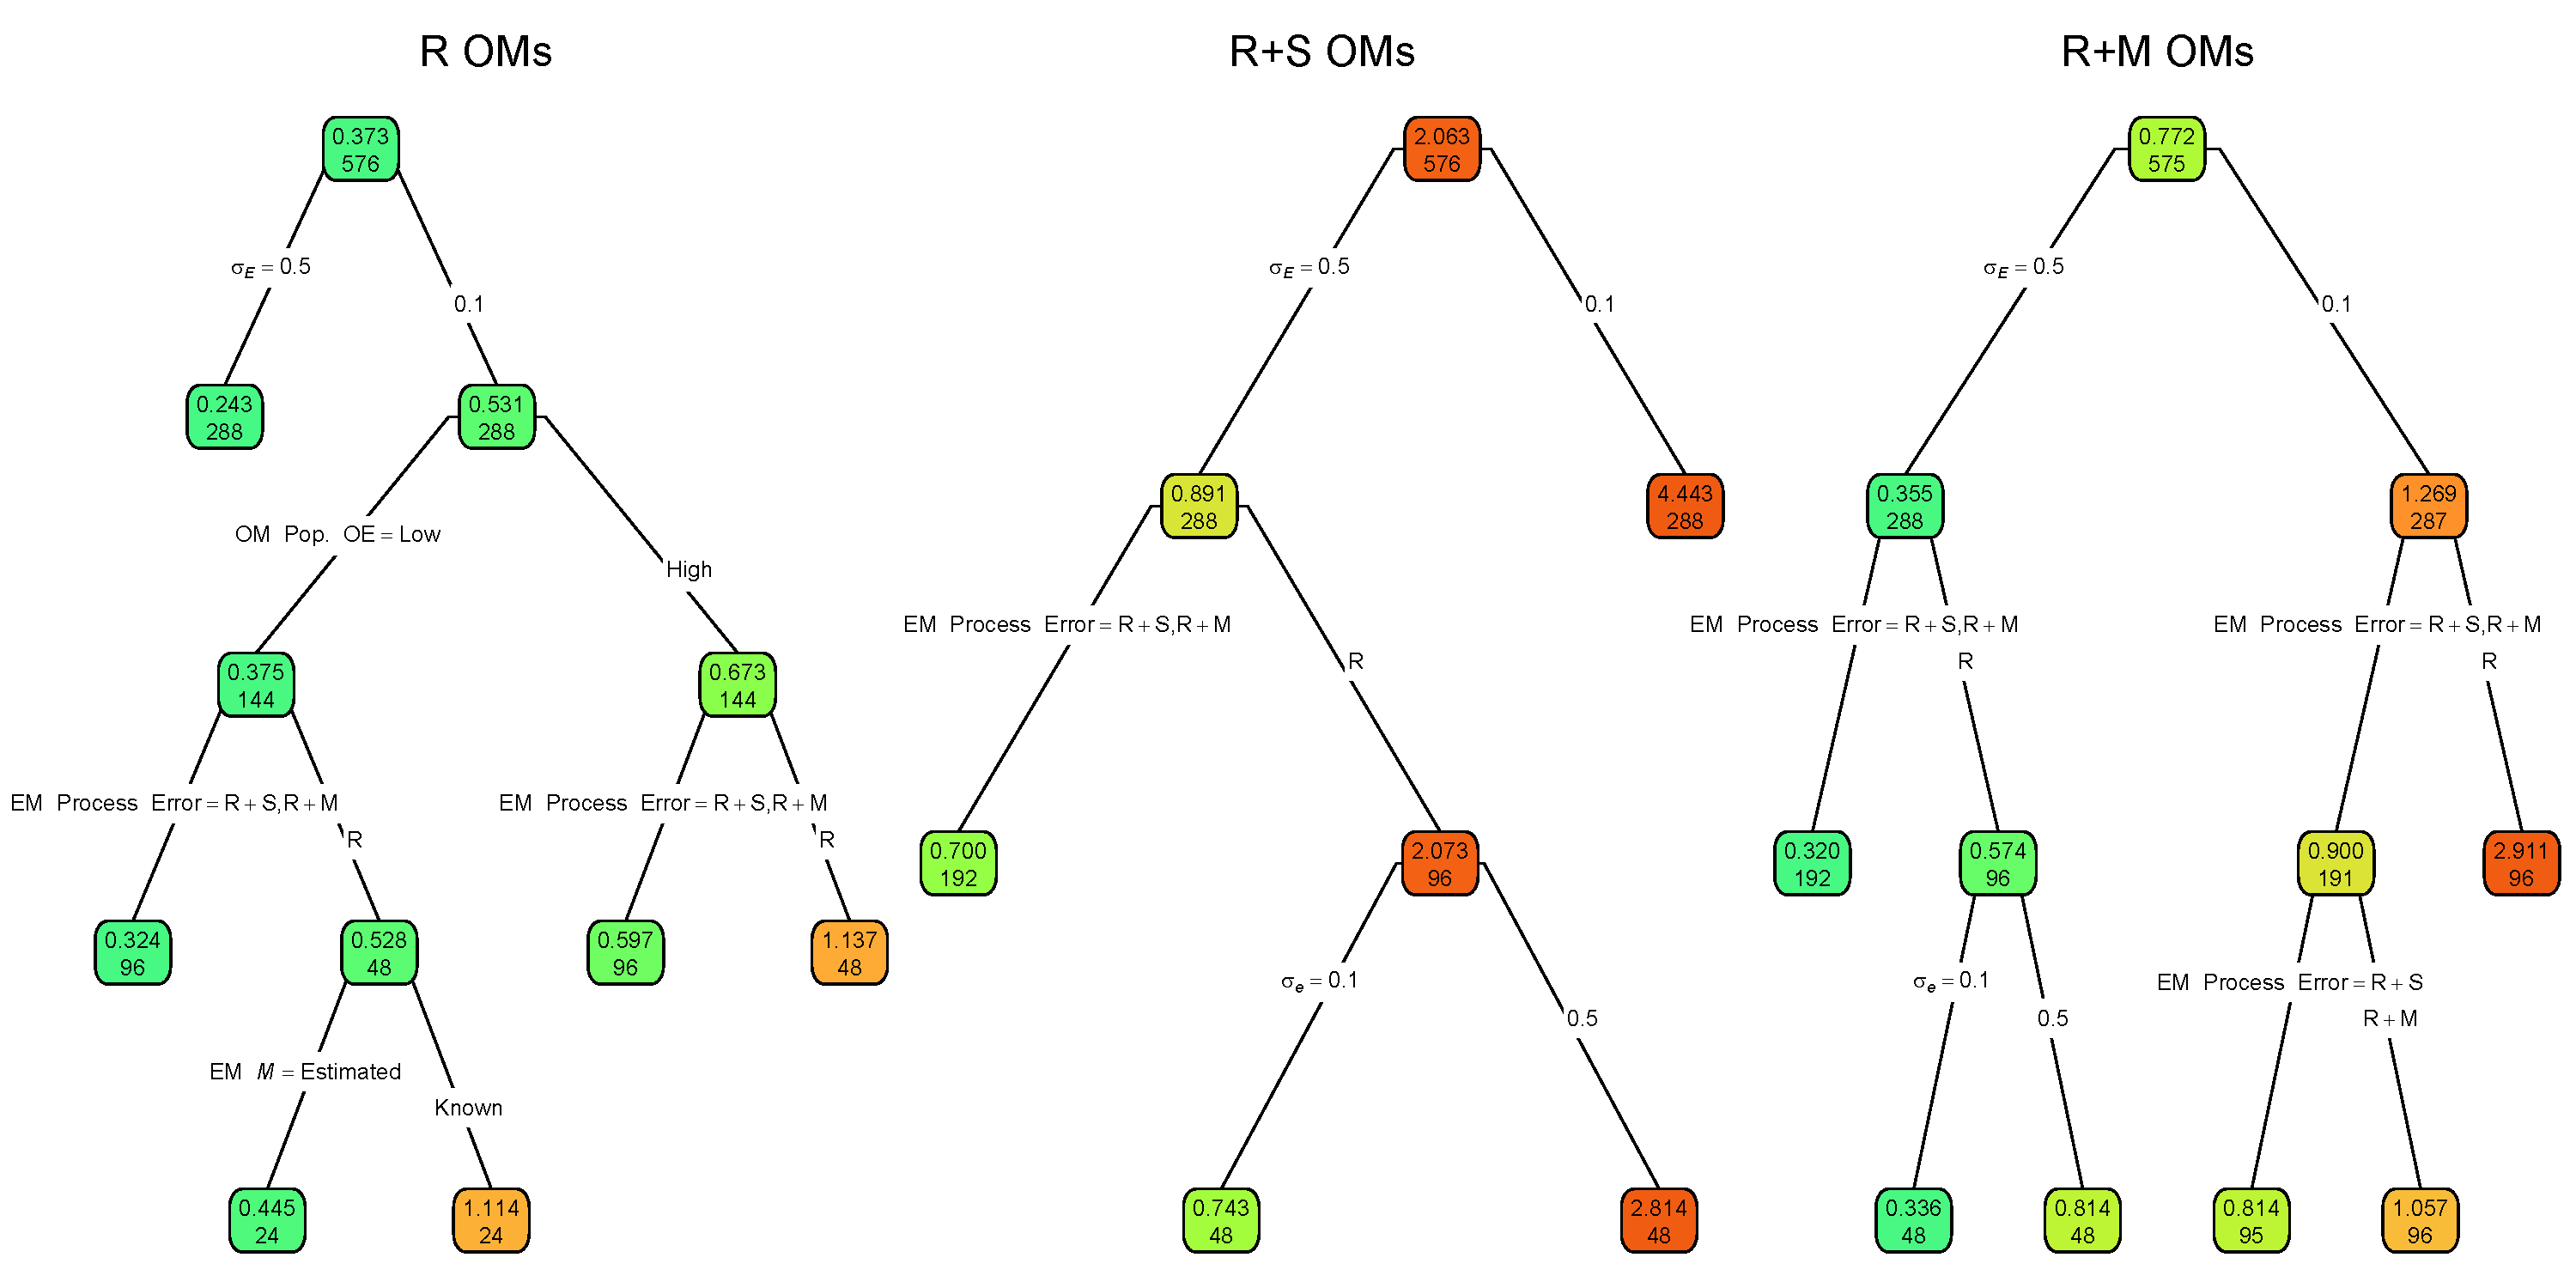
\includegraphics[width = 1.4\textwidth]{ecov_beta_rmse_regtree_plots}
\DIFaddendFL \end{center}
\caption{\DIFdelbeginFL \DIFdelFL{Root mean square error (}\DIFdelendFL \DIFaddbeginFL \DIFaddFL{Regression trees indicating primary factors determining reductions in sums of squares for the log-transformed }\DIFaddendFL RMSE \DIFdelbeginFL \DIFdelFL{) }\DIFdelendFL of \DIFdelbeginFL \DIFdelFL{estimates of }\DIFdelendFL covariate effect on \DIFdelbeginFL \DIFdelFL{natural mortality $\beta_E$ from fitting EMs }\DIFdelendFL \DIFaddbeginFL \DIFaddFL{$M$ ($\text{RMSE}\left(\widehat \beta_E\right)$) for operating models (OMs) }\DIFaddendFL with \DIFdelbeginFL \DIFdelFL{alternative }\DIFdelendFL process error \DIFdelbeginFL \DIFdelFL{assumptions }\DIFdelendFL \DIFaddbeginFL \DIFaddFL{on recruitment only (R), recruitment }\DIFaddendFL and \DIFdelbeginFL \DIFdelFL{treatment of median }\DIFdelendFL \DIFaddbeginFL \DIFaddFL{apparent survival (R+S), or recruitment and }\DIFaddendFL natural mortality (\DIFdelbeginFL \DIFdelFL{$e^\beta_M$ known or estimated}\DIFdelendFL \DIFaddbeginFL \DIFaddFL{R+M}\DIFaddendFL ). \DIFdelbeginFL \DIFdelFL{All OMs had low observation }\DIFdelendFL \DIFaddbeginFL \DIFaddFL{Each node shows the median }\DIFaddendFL error \DIFaddbeginFL \DIFaddFL{(top) }\DIFaddendFL and \DIFdelbeginFL \DIFdelFL{contrast in fishing mortality}\DIFdelendFL \DIFaddbeginFL \DIFaddFL{number of observations (bottom) for the corresponding subset}\DIFaddendFL . \DIFaddbeginFL \DIFaddFL{Lower or higher median RMSE are indicated by more green or red polygons, respectively.}\DIFaddendFL }\DIFdelbeginFL %DIFDELCMD < \label{beta_E_rmse}
%DIFDELCMD < %%%
\DIFdelendFL \DIFaddbeginFL \label{ecov_effect_rmse_regtree}
\DIFaddendFL \end{figure}
\end{landscape}

\DIFaddbegin \begin{table}
\caption{\DIFaddFL{For each OM process error source (columns), percent reduction in deviance for linear regression models fit to the log-transformed RMSE for estimates of the covariate effect on $M$  ($\text{RMSE}\left(\widehat \beta_E\right)$) with each OM and EM factor (rows) included individually, combined, and with second and third order interactions.}}\label{RMSE_ecov_beta_PRD_table}
{\begin{center}
\begin{tabular}{lrrr}
\hline\hline
\multicolumn{1}{l}{\DIFaddFL{Factor}}&\multicolumn{1}{c}{\DIFaddFL{R}}&\multicolumn{1}{c}{\DIFaddFL{R+S}}&\multicolumn{1}{c}{\DIFaddFL{R+M}}\tabularnewline
\hline
\DIFaddFL{OM $F$ history}& \DIFaddFL{0.50}& \DIFaddFL{0.11}& \DIFaddFL{0.12}\tabularnewline
\DIFaddFL{OM Obs. Error}&\DIFaddFL{12.04}& \DIFaddFL{5.66}& \DIFaddFL{0.36}\tabularnewline
\DIFaddFL{$OM \sigma_e$}& \DIFaddFL{0.87}& \DIFaddFL{5.78}& \DIFaddFL{2.60}\tabularnewline
\DIFaddFL{$OM \sigma_E$}&\DIFaddFL{15.85}&\DIFaddFL{24.18}&\DIFaddFL{24.26}\tabularnewline
\DIFaddFL{$OM \rho_{E}$}& \DIFaddFL{0.36}& \DIFaddFL{0.82}& \DIFaddFL{0.34}\tabularnewline
\DIFaddFL{OM $\beta_{E}$}& \DIFaddFL{6.72}& \DIFaddFL{0.07}& \DIFaddFL{0.96}\tabularnewline
\DIFaddFL{EM Process Error}& \DIFaddFL{6.49}&\DIFaddFL{11.31}&\DIFaddFL{11.98}\tabularnewline
\DIFaddFL{EM $M$ assumption}& \DIFaddFL{0.04}& \DIFaddFL{0.64}& \DIFaddFL{0.07}\tabularnewline
\DIFaddFL{All factors}&\DIFaddFL{42.87}&\DIFaddFL{48.58}&\DIFaddFL{40.65}\tabularnewline
\DIFaddFL{+ All Two Way}&\DIFaddFL{67.34}&\DIFaddFL{74.09}&\DIFaddFL{61.74}\tabularnewline
\DIFaddFL{+ All Three Way}&\DIFaddFL{79.42}&\DIFaddFL{82.75}&\DIFaddFL{71.92}\tabularnewline
\hline
\end{tabular}\end{center}
}
\end{table}

\DIFaddend \begin{landscape}
\begin{figure}
\begin{center}
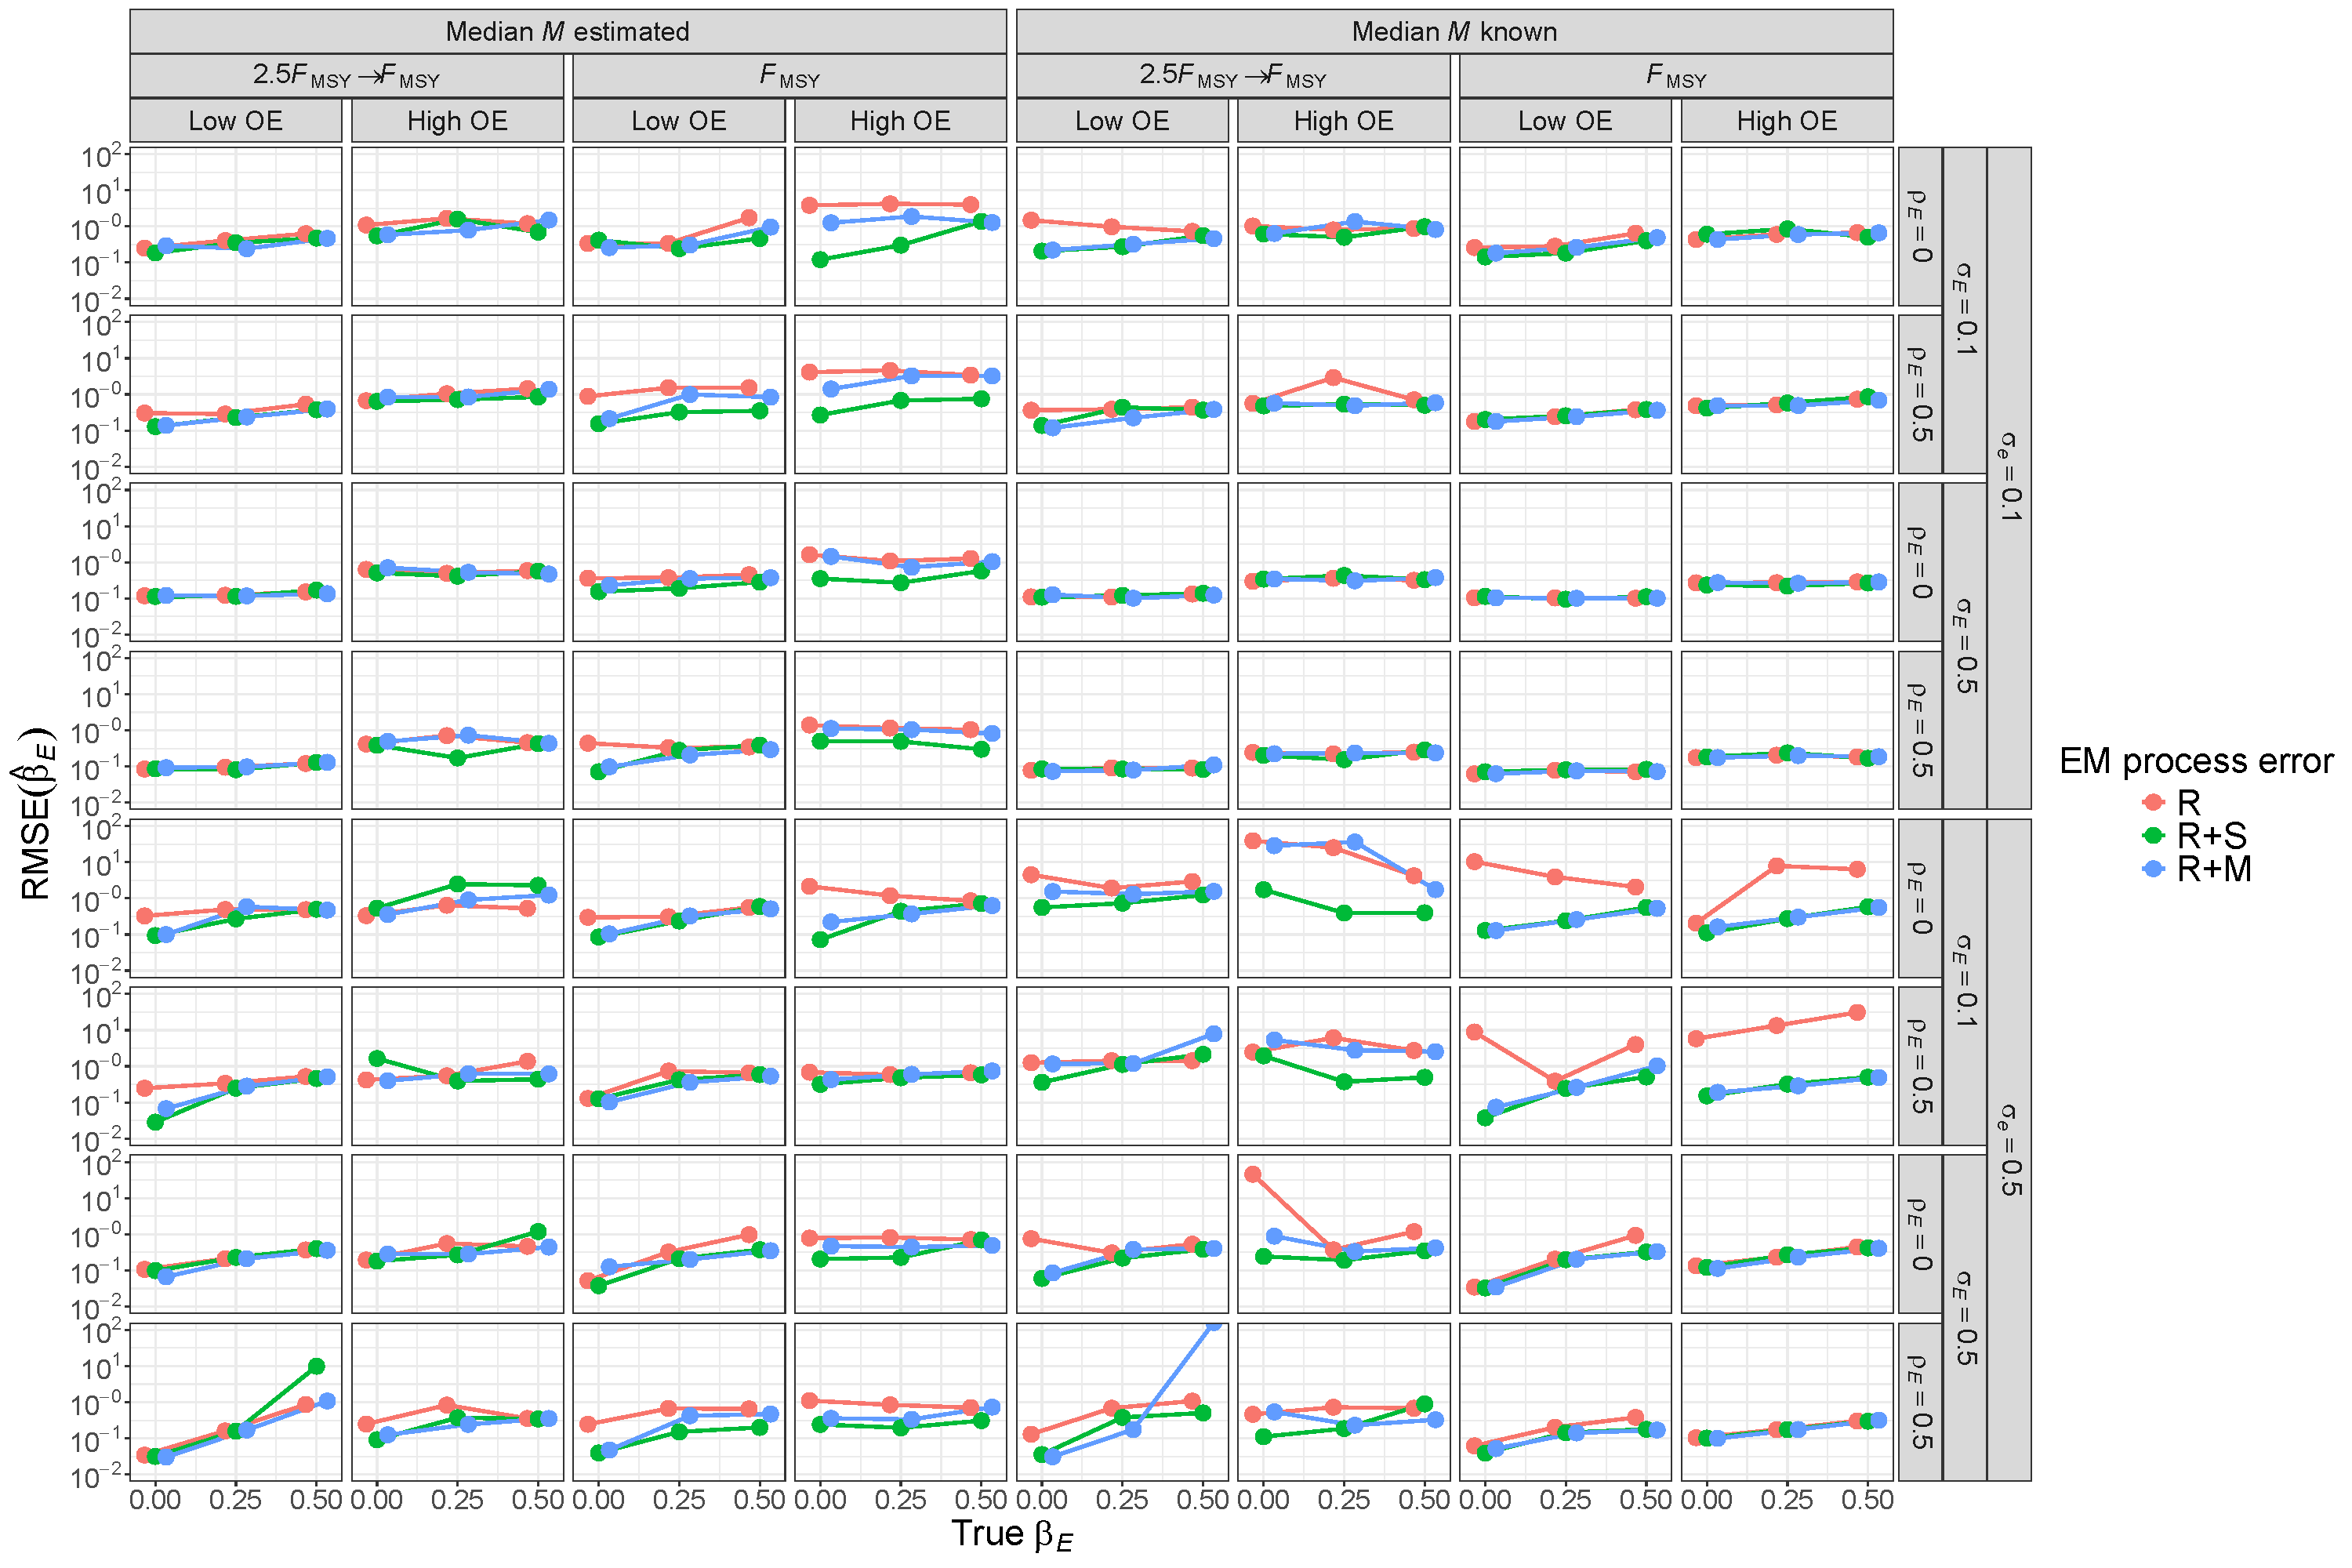
\includegraphics[height = \textheight]{beta_E_rmse_Rom}
\end{center}
\caption{For R OMs, \DIFdelbeginFL \DIFdelFL{root mean square error (}\DIFdelendFL RMSE \DIFdelbeginFL \DIFdelFL{) }\DIFdelendFL of estimates of covariate effect on \DIFdelbeginFL \DIFdelFL{natural mortality }\DIFdelendFL \DIFaddbeginFL \DIFaddFL{$M$ (}\DIFaddendFL $\beta_E$\DIFaddbeginFL \DIFaddFL{) }\DIFaddendFL from fitting EMs with alternative process error assumptions and treatment of median \DIFdelbeginFL \DIFdelFL{natural mortality }\DIFdelendFL \DIFaddbeginFL \DIFaddFL{$M$ }\DIFaddendFL ($e^\beta_M$ known or estimated). }\label{beta_E_rmse_Rom}
\end{figure}
\end{landscape}

\begin{landscape}
\begin{figure}
\begin{center}
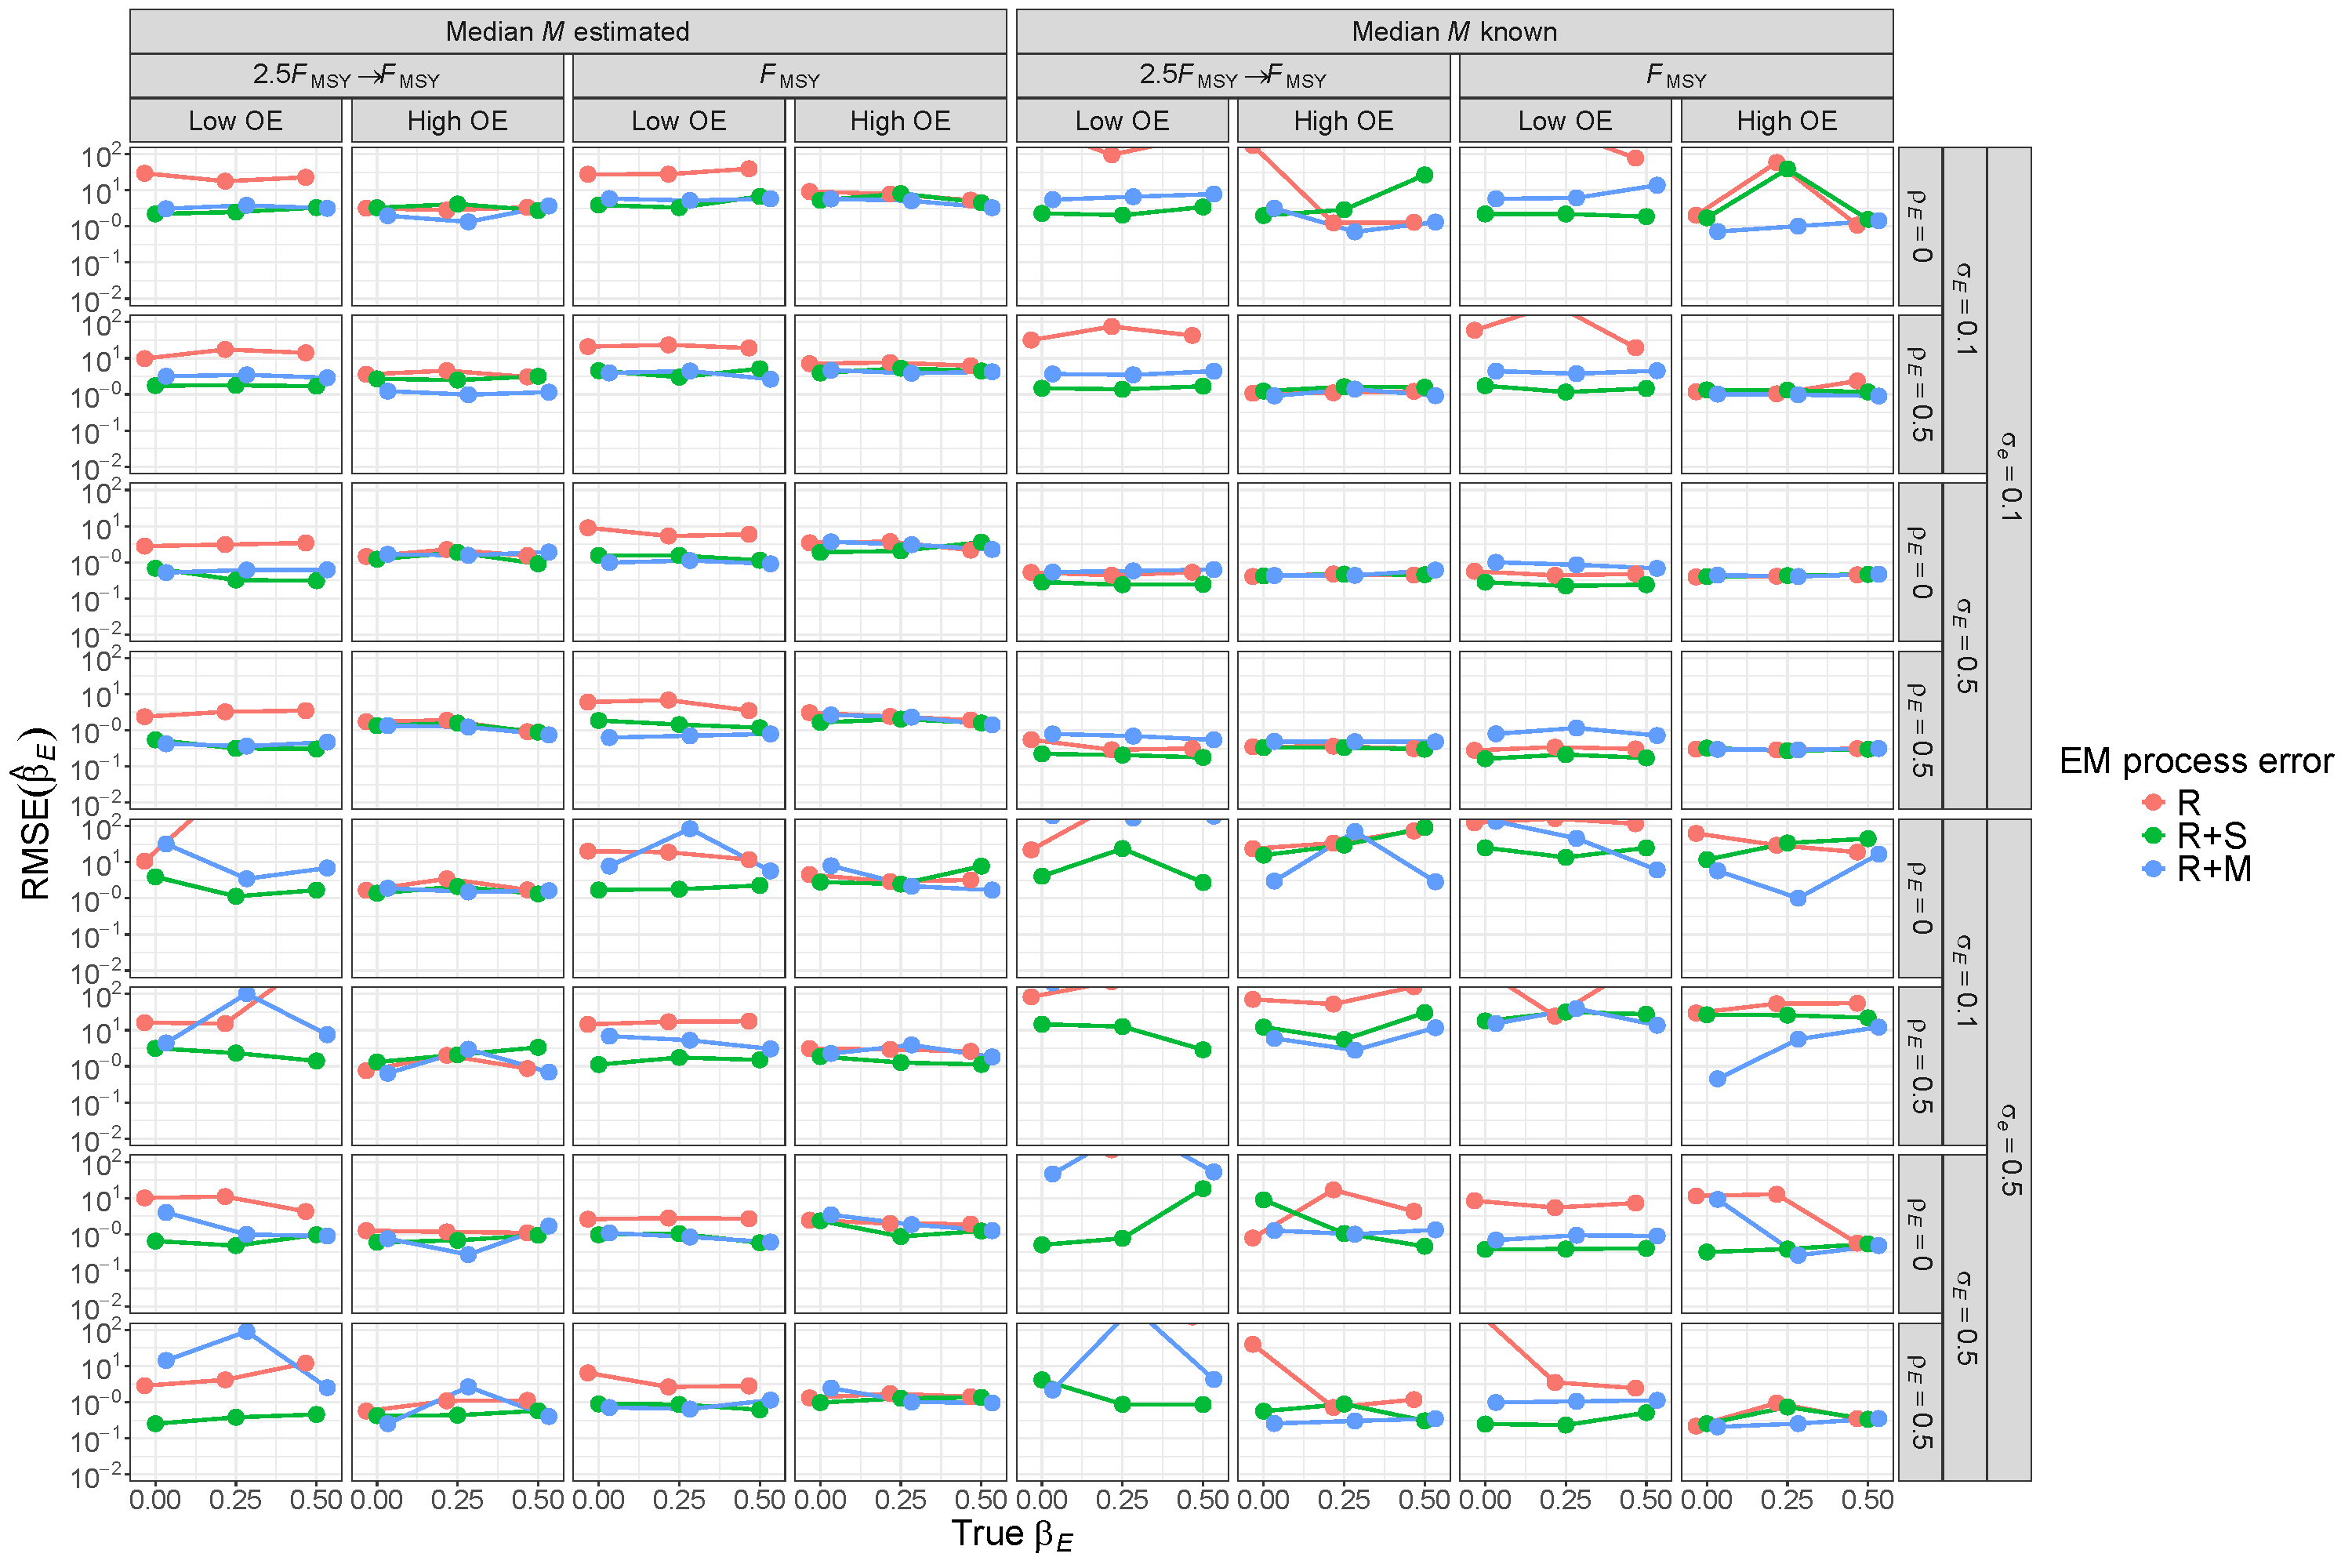
\includegraphics[height = \textheight]{beta_E_rmse_RSom}
\end{center}
\caption{For R+S OMs, \DIFdelbeginFL \DIFdelFL{root mean square error (}\DIFdelendFL RMSE \DIFdelbeginFL \DIFdelFL{) }\DIFdelendFL of estimates of covariate effect on \DIFdelbeginFL \DIFdelFL{natural mortality }\DIFdelendFL \DIFaddbeginFL \DIFaddFL{$M$ (}\DIFaddendFL $\beta_E$\DIFaddbeginFL \DIFaddFL{) }\DIFaddendFL from fitting EMs with alternative process error assumptions and treatment of median \DIFdelbeginFL \DIFdelFL{natural mortality }\DIFdelendFL \DIFaddbeginFL \DIFaddFL{$M$ }\DIFaddendFL ($e^\beta_M$ known or estimated). }\label{beta_E_rmse_RSom}
\end{figure}
\end{landscape}

\begin{landscape}
\begin{figure}
\begin{center}
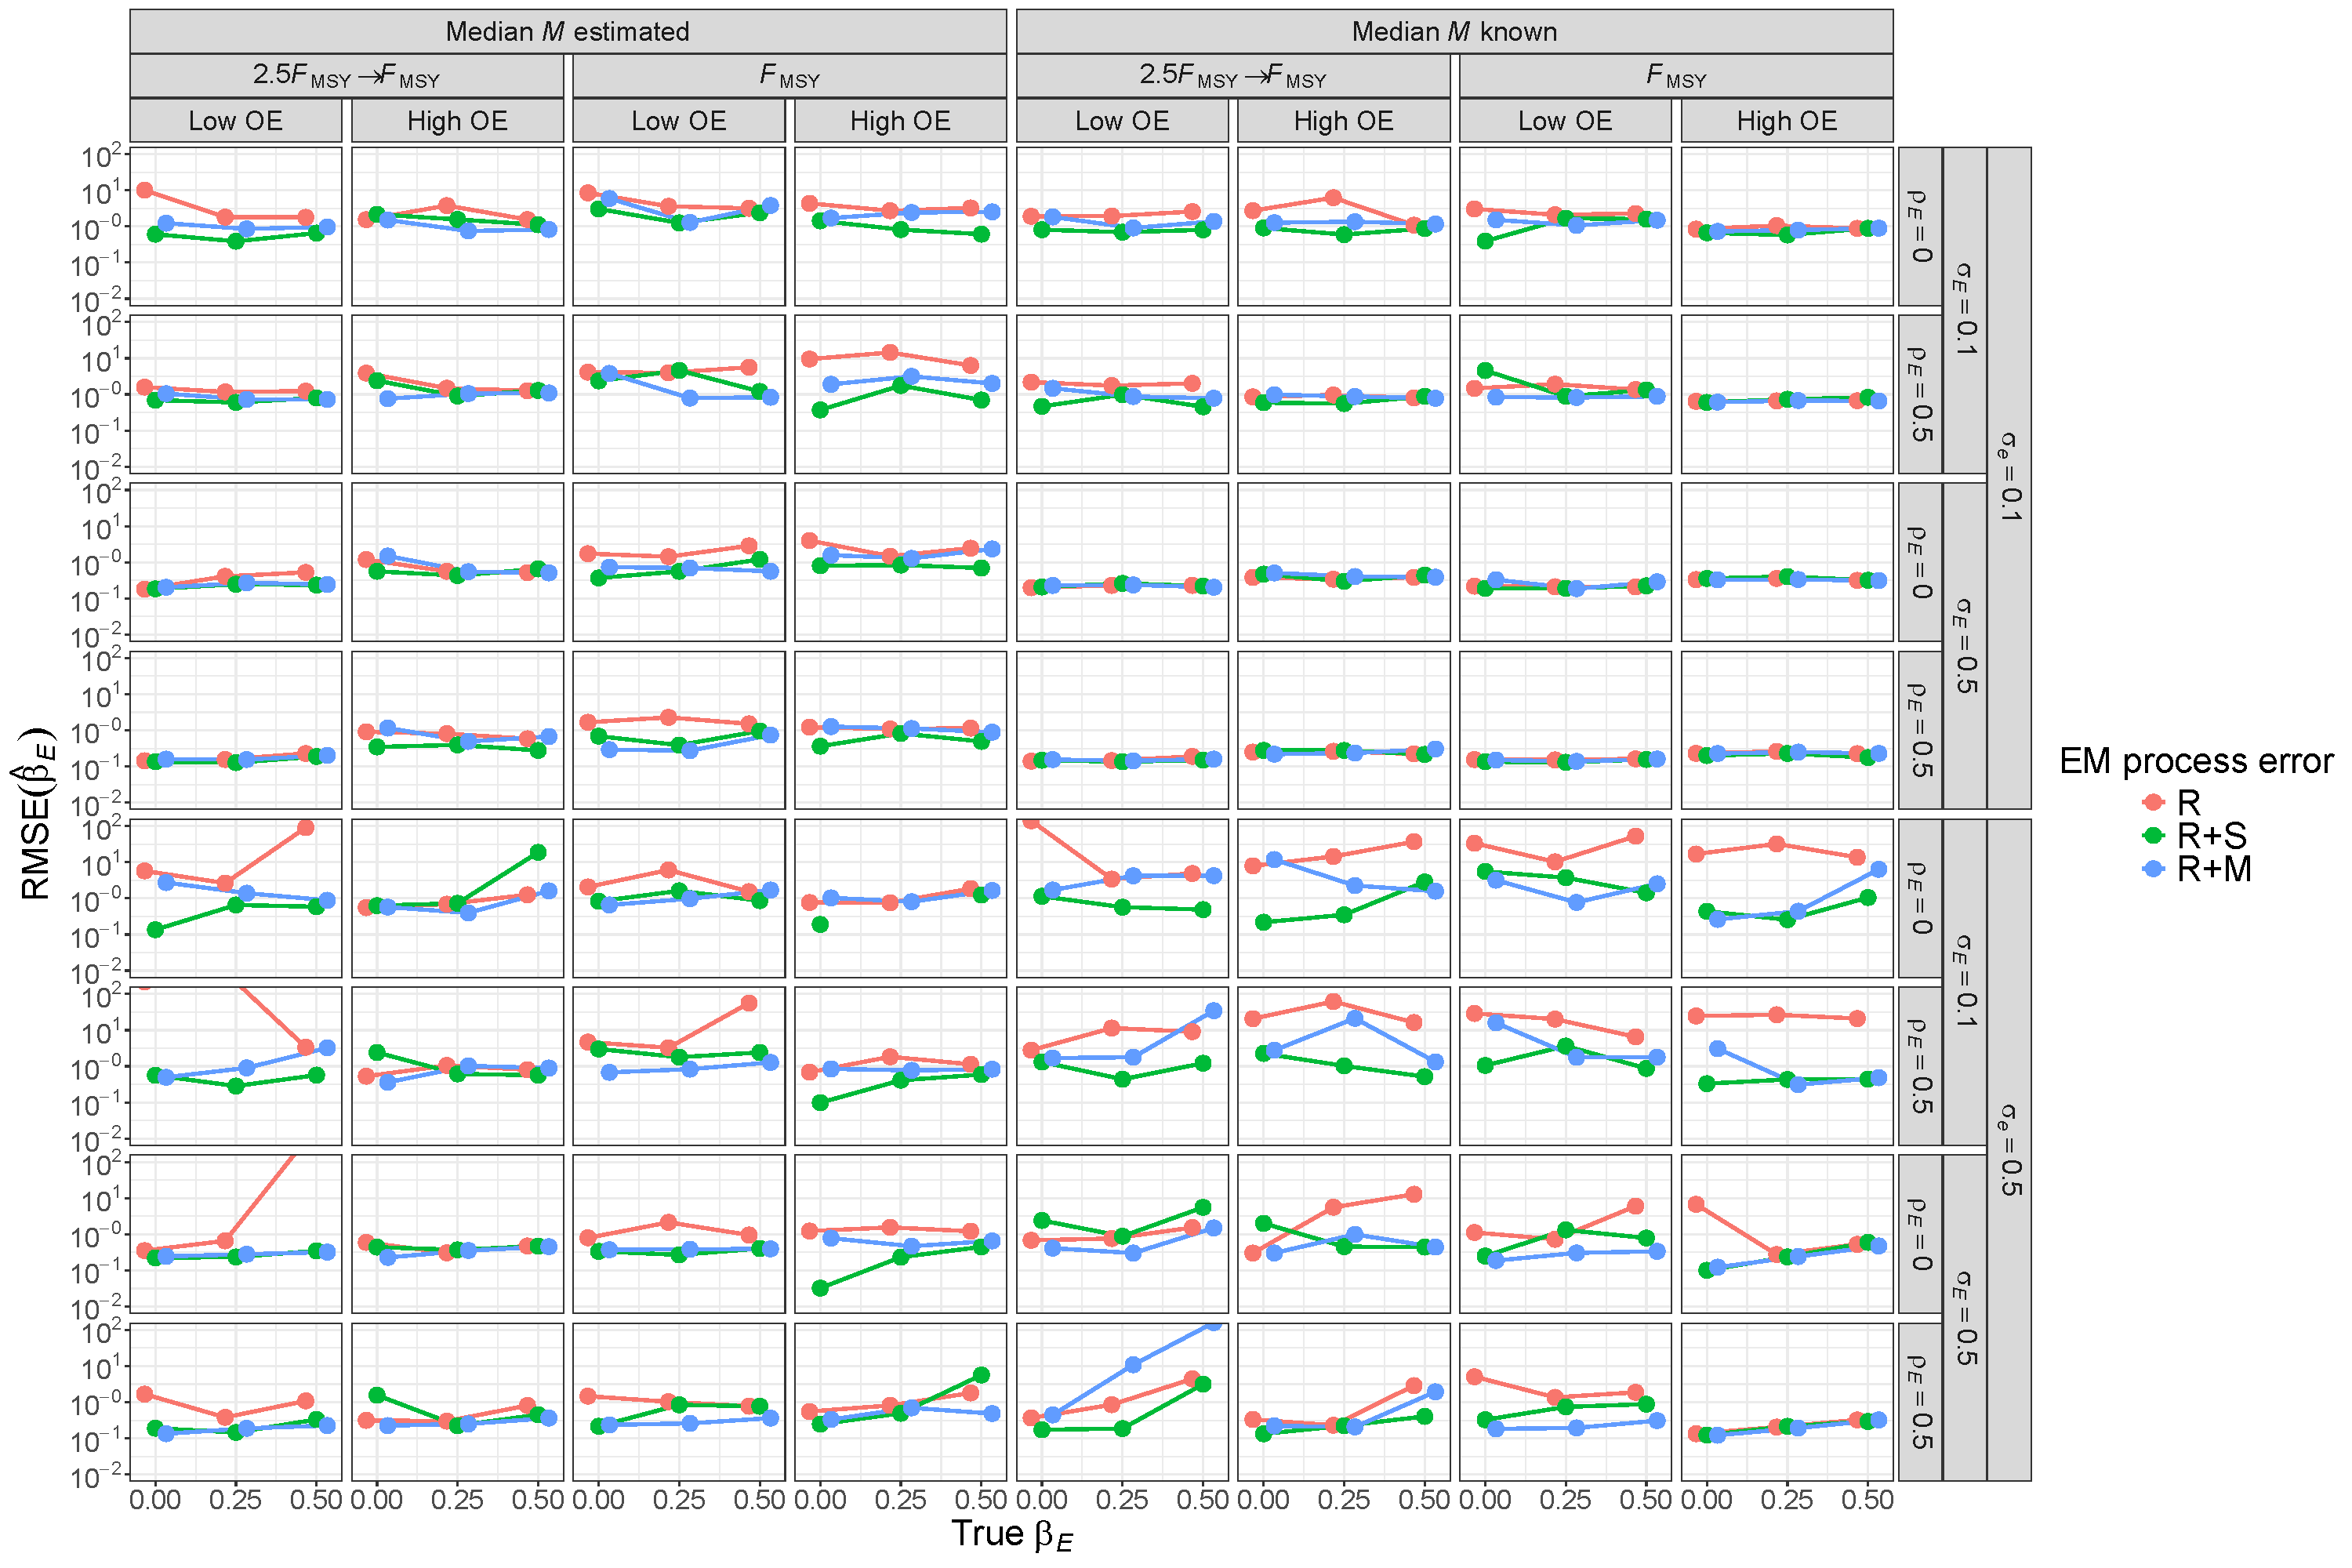
\includegraphics[height = \textheight]{beta_E_rmse_RMom}
\end{center}
\caption{For R+M OMs, \DIFdelbeginFL \DIFdelFL{root mean square error (}\DIFdelendFL RMSE \DIFdelbeginFL \DIFdelFL{) }\DIFdelendFL of estimates of covariate effect on \DIFdelbeginFL \DIFdelFL{natural mortality }\DIFdelendFL \DIFaddbeginFL \DIFaddFL{$M$ (}\DIFaddendFL $\beta_E$\DIFaddbeginFL \DIFaddFL{) }\DIFaddendFL from fitting EMs with alternative process error assumptions and treatment of median \DIFdelbeginFL \DIFdelFL{natural mortality }\DIFdelendFL \DIFaddbeginFL \DIFaddFL{$M$ }\DIFaddendFL ($e^\beta_M$ known or estimated). }\label{beta_E_rmse_RMom}
\end{figure}
\end{landscape}

\DIFdelbegin %DIFDELCMD < \hypertarget{covariate-effect-estimate-and-standard-error-example}{%
%DIFDELCMD < \subsection*{Covariate effect estimate and standard error example}\label{covariate-effect-estimate-and-standard-error-example}}
%DIFDELCMD < %%%
\DIFdelend \DIFaddbegin \subsection*{\DIFadd{Covariate effect estimate and standard error example}}\label{covariate-effect-estimate-and-standard-error-example}
\DIFaddend \addcontentsline{toc}{subsection}{Covariate effect estimate and standard error example}

\begin{landscape}
\begin{figure}
\begin{center}
\DIFdelbeginFL %DIFDELCMD < 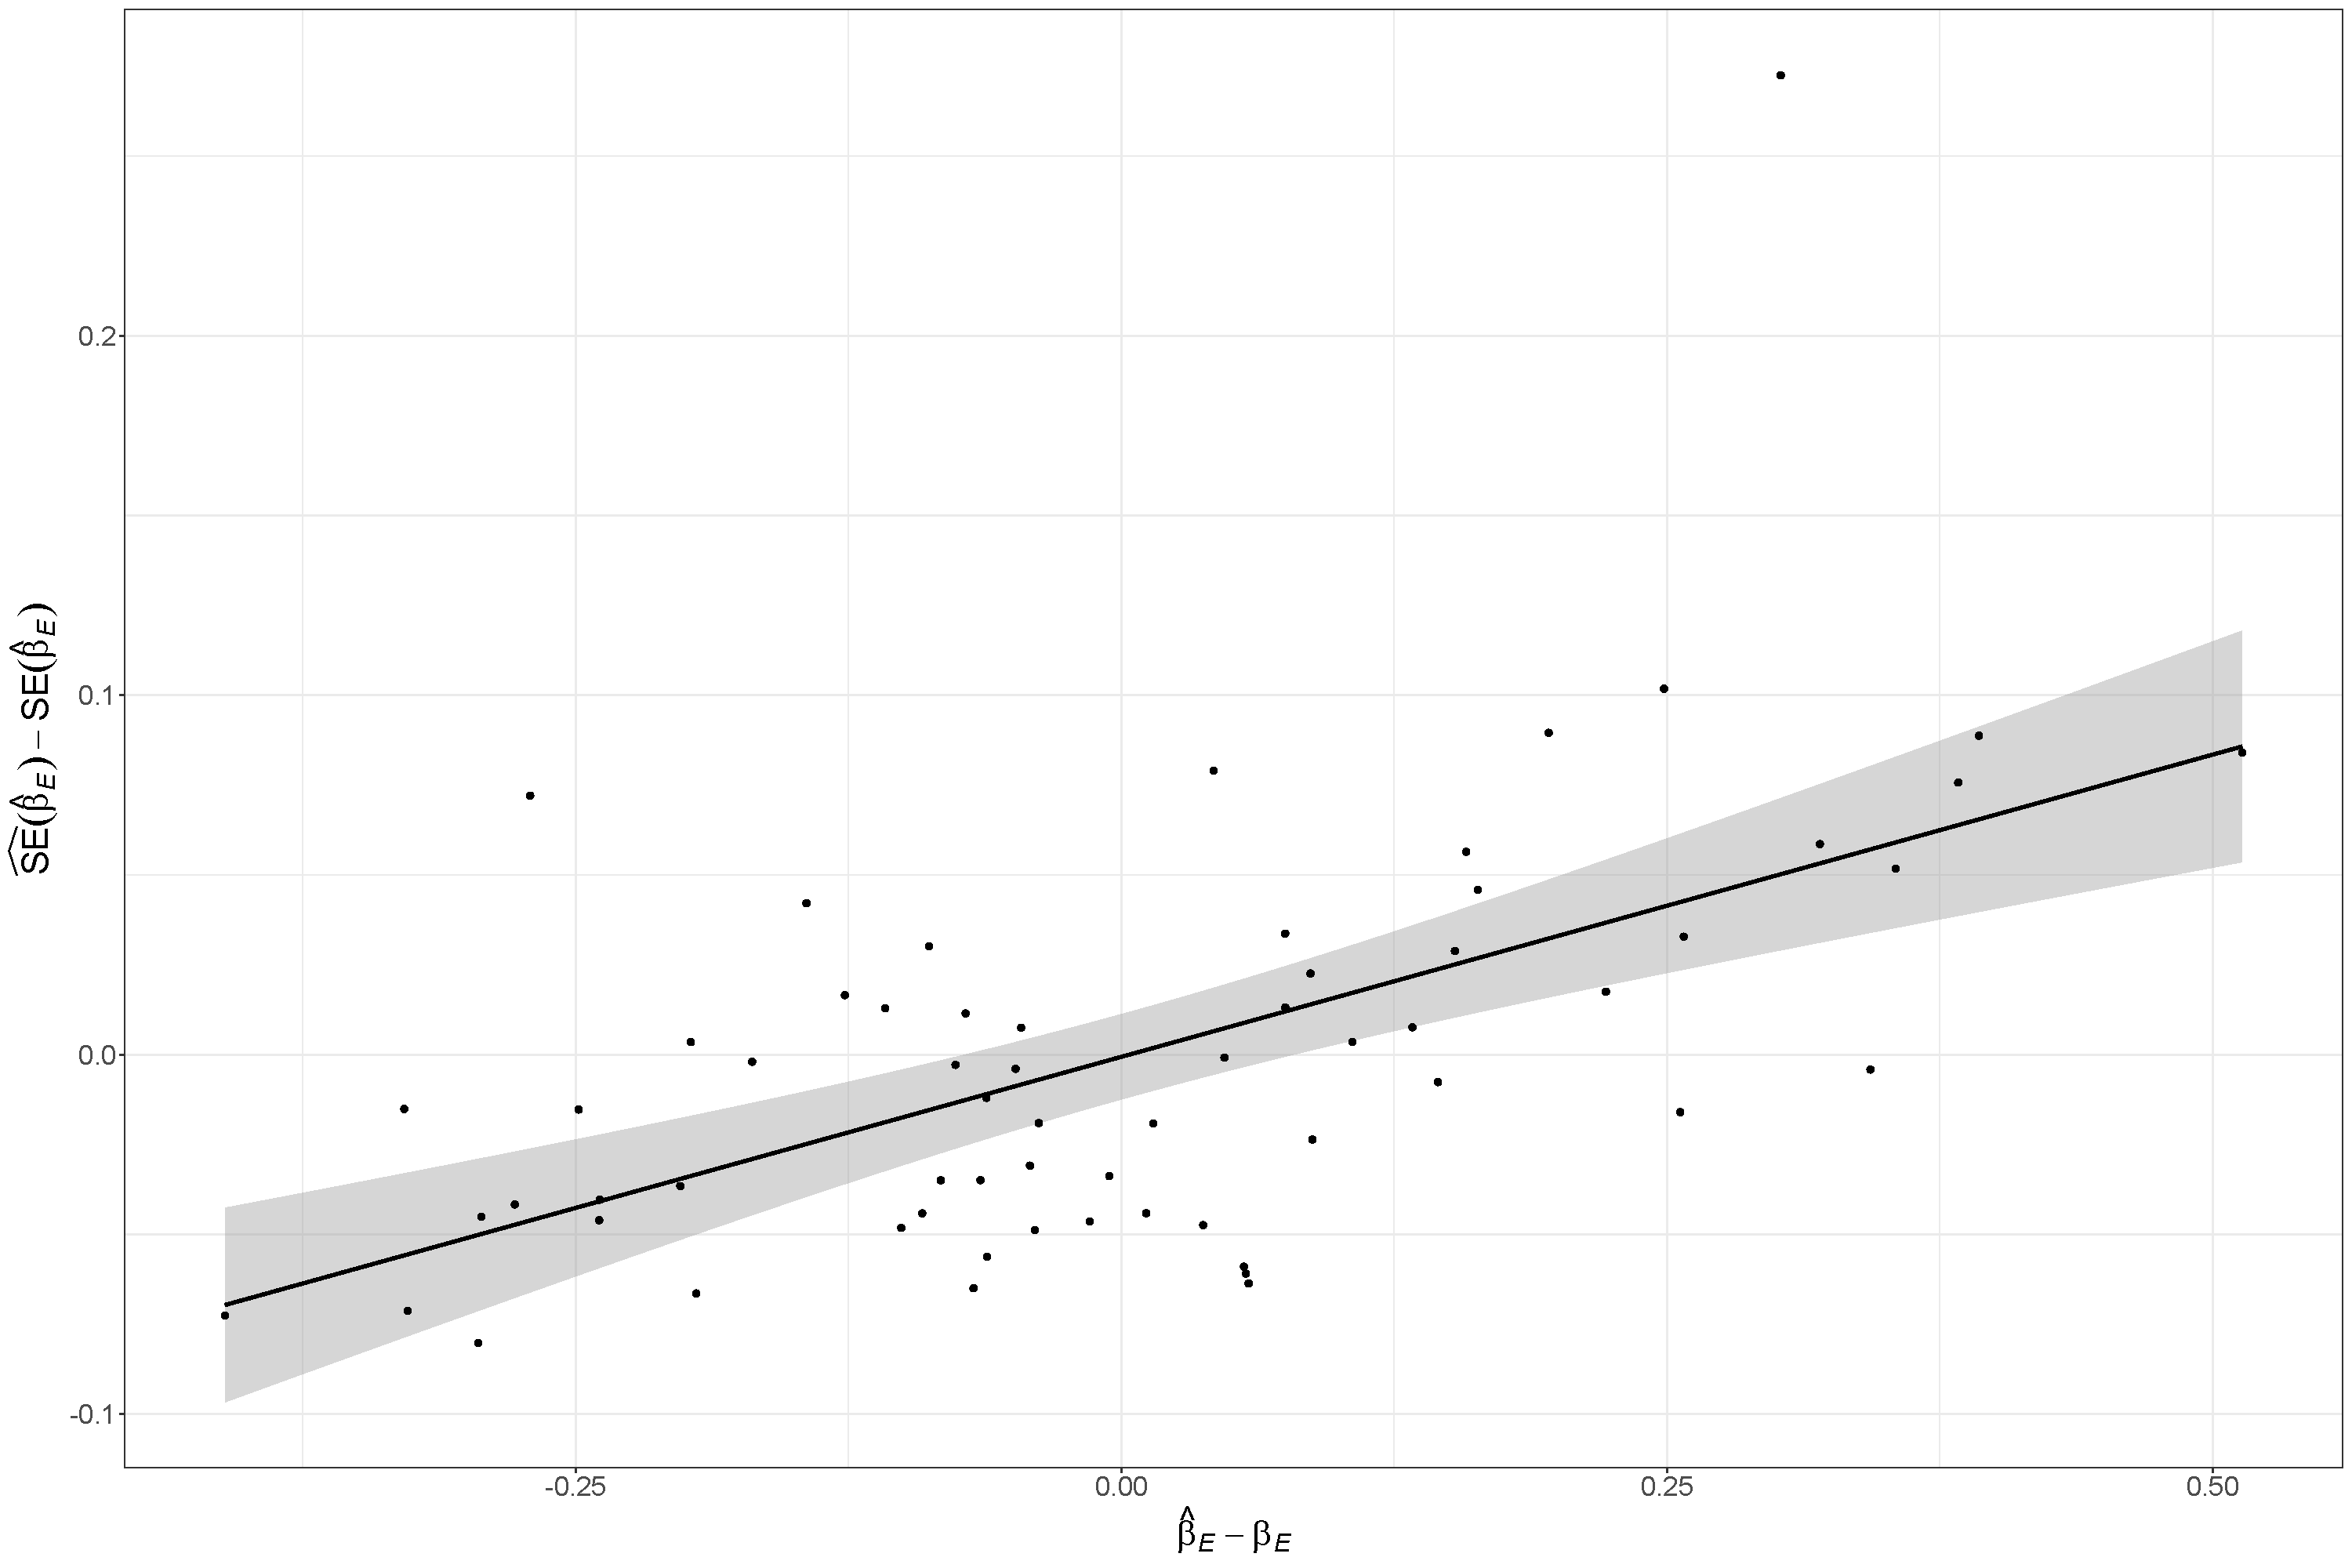
\includegraphics[height = \textheight]{om_69_em_5_beta_E_se_beta_E_lm_plot}
%DIFDELCMD < %%%
\DIFdelendFL \DIFaddbeginFL 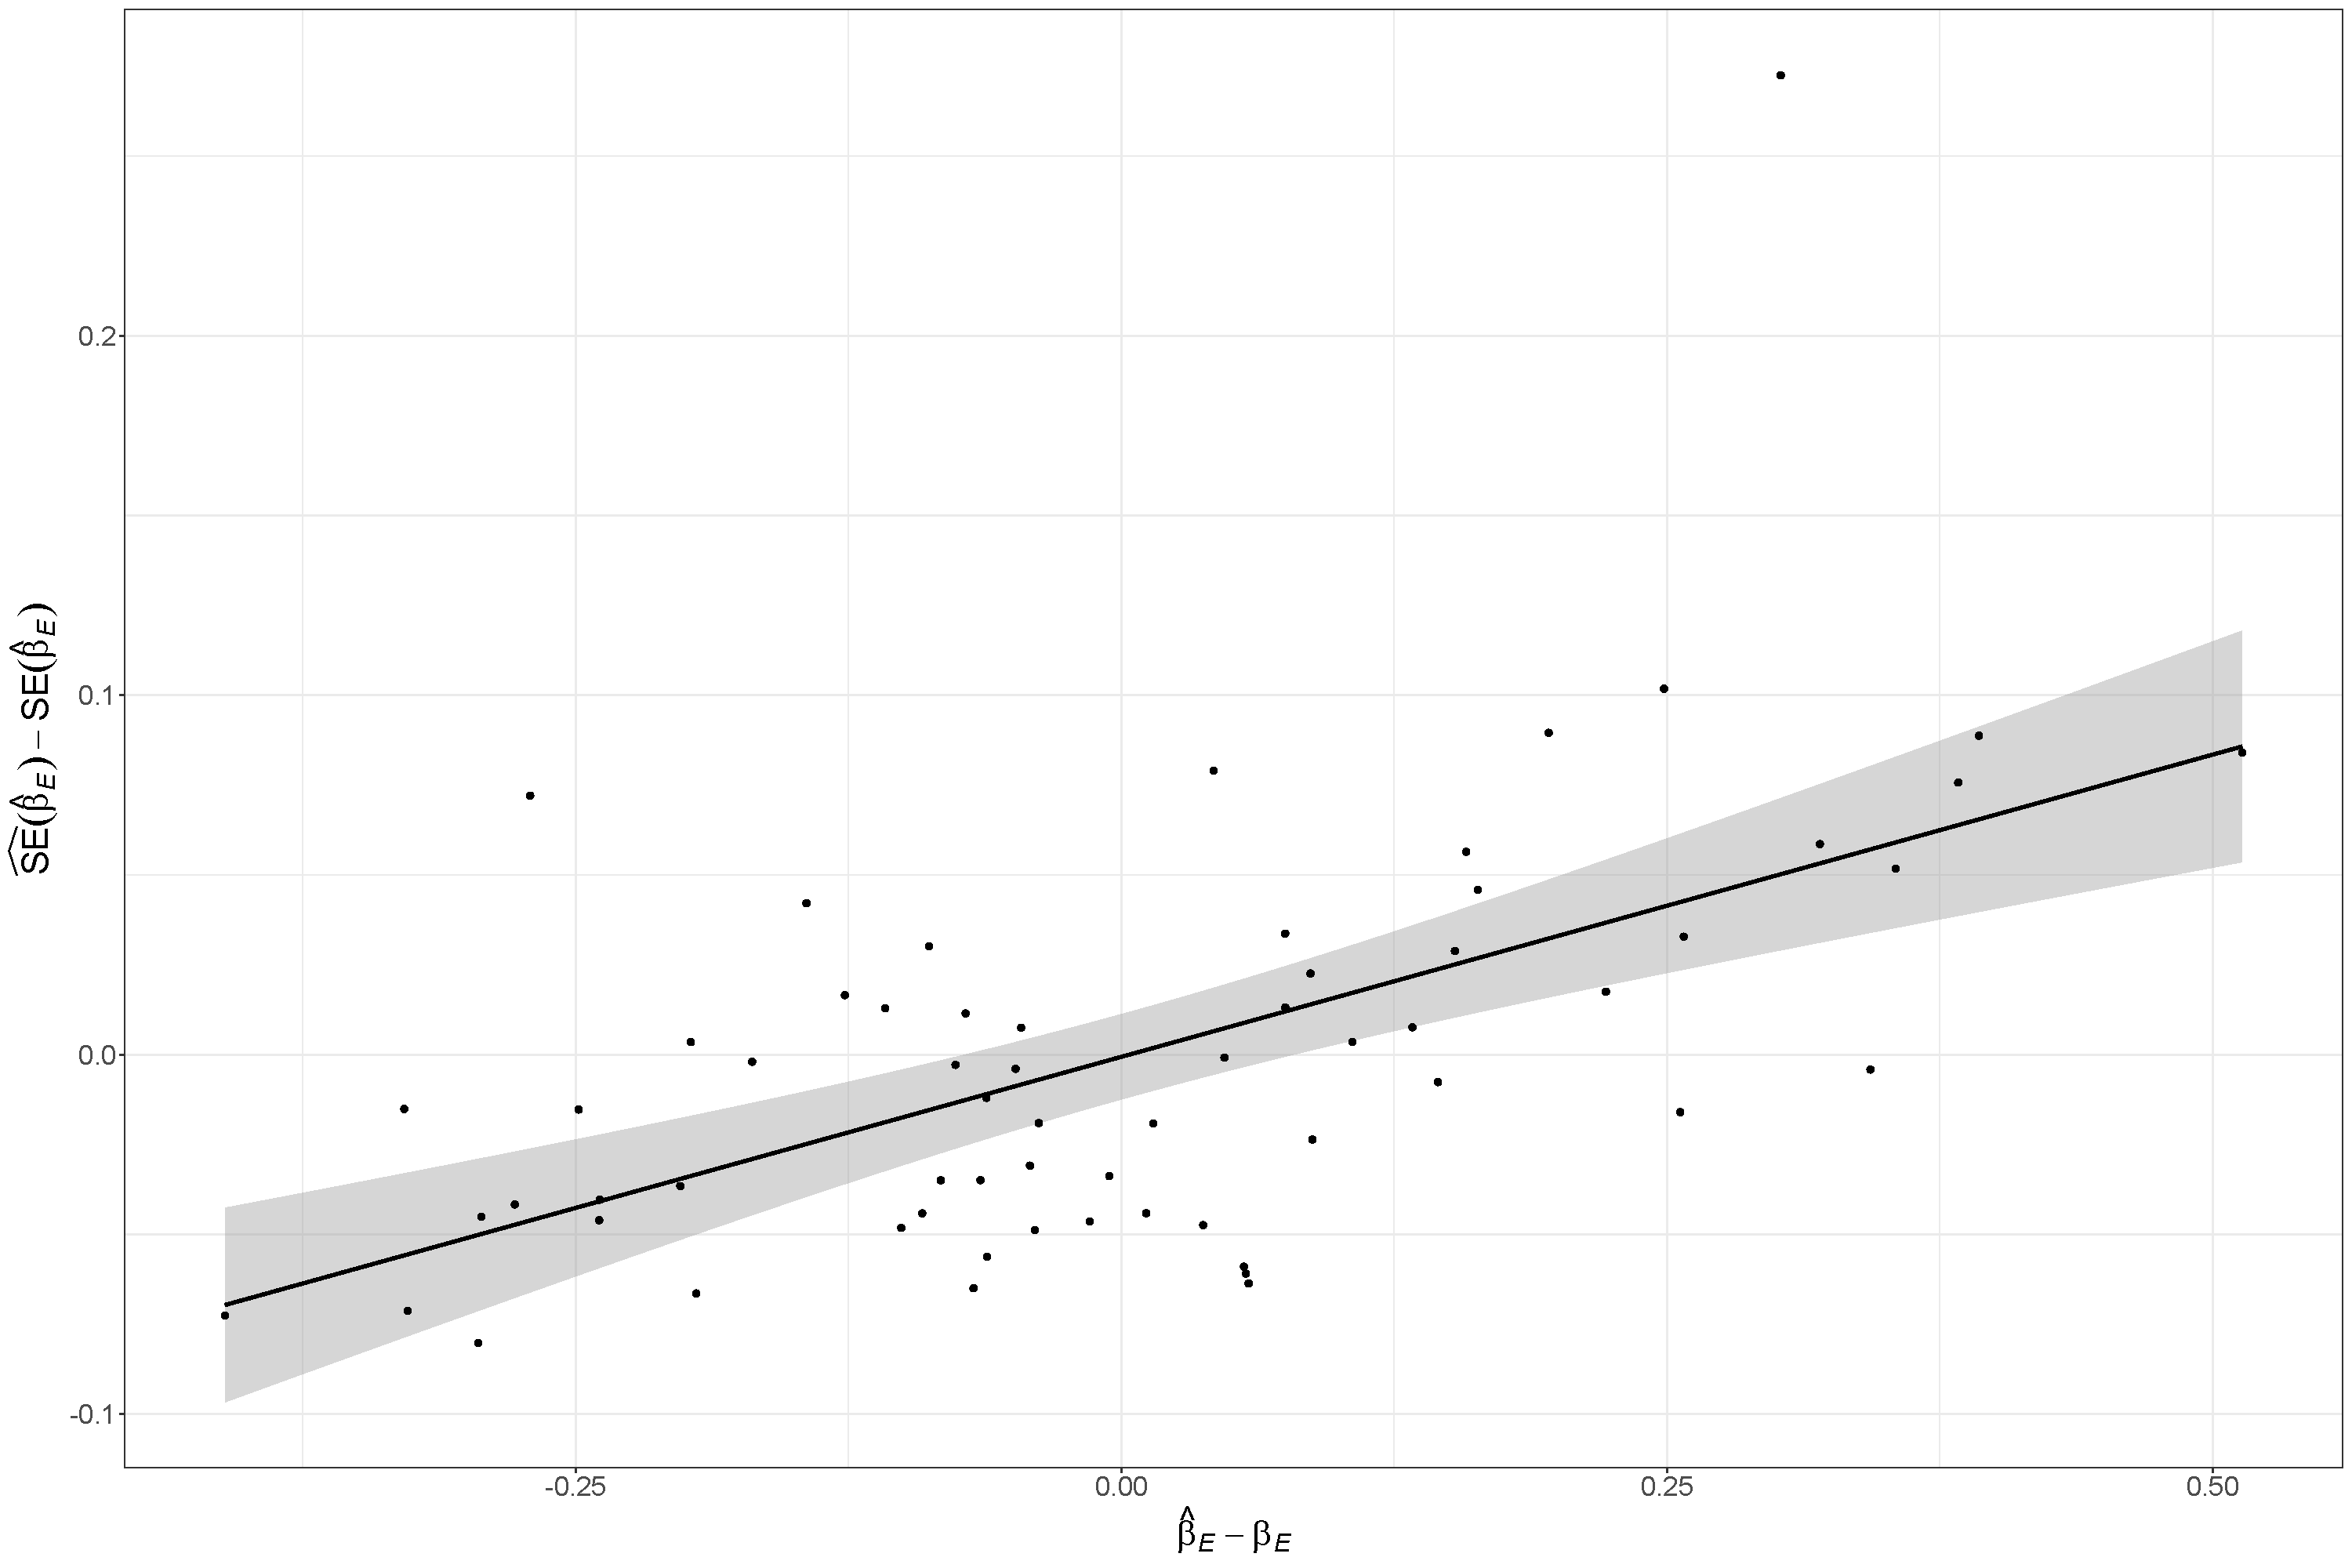
\includegraphics[height = 0.9\textheight]{om_69_em_5_beta_E_se_beta_E_lm_plot}
\DIFaddendFL \end{center}
\caption{Positive correlation of covariate effect estimates and Hessian-based standard error estimates for EM that also estimates the median \DIFdelbeginFL \DIFdelFL{natural mortality }\DIFdelendFL \DIFaddbeginFL \DIFaddFL{$M$ }\DIFaddendFL parameter \DIFaddbeginFL \DIFaddFL{($\beta_M$) }\DIFaddendFL and has correct R+M process error assumption fitted to simulated data from the OM with R+M process errors, temporal contrast in fishing pressure, low observation uncertainty for both population ($Low OE$) and covariate observations ($\sigma_e = 0.1$), high and uncorrelated temporal variability in the true covariate ($\sigma_E = 0.5$ and $\rho_E = 0$), and the strongest covariate effect on \DIFdelbeginFL \DIFdelFL{natural mortality }\DIFdelendFL \DIFaddbeginFL \DIFaddFL{$M$ }\DIFaddendFL ($\beta_E = 0.5$).}\label{ex_lm_beta_E_SE_beta_E}
\end{figure}
\end{landscape}

\DIFdelbegin %DIFDELCMD < \hypertarget{median-natural-mortality-parameter-bias}{%
%DIFDELCMD < \subsection*{Median Natural mortality parameter bias}\label{median-natural-mortality-parameter-bias}}
%DIFDELCMD < %%%
\DIFdelend \DIFaddbegin \subsection*{\DIFadd{Median Natural mortality parameter bias}}\label{median-natural-mortality-parameter-bias}
\DIFaddend \addcontentsline{toc}{subsection}{Median Natural mortality parameter bias}

\DIFaddbegin \begin{table}
\caption{\DIFaddFL{For each OM process error source (columns), percent reduction in deviance for linear regression models fit to errors in estimation of the median $M$ parameter ($\beta_M$) with each OM and EM factor (rows) included individually, combined, and with second and third order interactions. Includes results from all unconverged and converged models.}}\label{bias_median_M_complete_PRD_table}
{\begin{center}
\begin{tabular}{lrrr}
\hline\hline
\multicolumn{1}{l}{\DIFaddFL{Factor}}&\multicolumn{1}{c}{\DIFaddFL{R}}&\multicolumn{1}{c}{\DIFaddFL{R+S}}&\multicolumn{1}{c}{\DIFaddFL{R+M}}\tabularnewline
\hline
\DIFaddFL{OM $F$ history}&\DIFaddFL{\textless  0.01}&\DIFaddFL{\textless  0.01}&\DIFaddFL{\textless  0.01}\tabularnewline
\DIFaddFL{OM Obs. Error}&\DIFaddFL{\textless  0.01}&\DIFaddFL{\textless  0.01}&\DIFaddFL{\textless  0.01}\tabularnewline
\DIFaddFL{OM $\sigma_e$}&\DIFaddFL{\textless  0.01}&\DIFaddFL{\textless  0.01}&\DIFaddFL{\textless  0.01}\tabularnewline
\DIFaddFL{OM $\sigma_E$}&\DIFaddFL{\textless  0.01}&\DIFaddFL{\textless  0.01}&\DIFaddFL{\textless  0.01}\tabularnewline
\DIFaddFL{OM $\rho_{E}$}&\DIFaddFL{\textless  0.01}&\DIFaddFL{\textless  0.01}&\DIFaddFL{\textless  0.01}\tabularnewline
\DIFaddFL{OM $\beta_{E}$}&\DIFaddFL{\textless  0.01}&\DIFaddFL{\textless  0.01}&\DIFaddFL{0.01}\tabularnewline
\DIFaddFL{EM Convergence}&\DIFaddFL{\textless  0.01}&\DIFaddFL{0.01}&\DIFaddFL{0.01}\tabularnewline
\DIFaddFL{EM Process Error}&\DIFaddFL{\textless  0.01}&\DIFaddFL{0.01}&\DIFaddFL{0.01}\tabularnewline
\DIFaddFL{EM $\beta_{E}$ assumption}&\DIFaddFL{\textless  0.01}&\DIFaddFL{\textless  0.01}&\DIFaddFL{\textless  0.01}\tabularnewline
\DIFaddFL{All factors}&\DIFaddFL{0.02}&\DIFaddFL{0.02}&\DIFaddFL{0.05}\tabularnewline
\DIFaddFL{+ All Two Way}&\DIFaddFL{0.15}&\DIFaddFL{0.15}&\DIFaddFL{0.24}\tabularnewline
\DIFaddFL{+ All Three Way}&\DIFaddFL{0.57}&\DIFaddFL{0.54}&\DIFaddFL{0.73}\tabularnewline
\hline
\end{tabular}\end{center}
}
\end{table}

\DIFaddend \begin{landscape}
\begin{figure}
\begin{center}
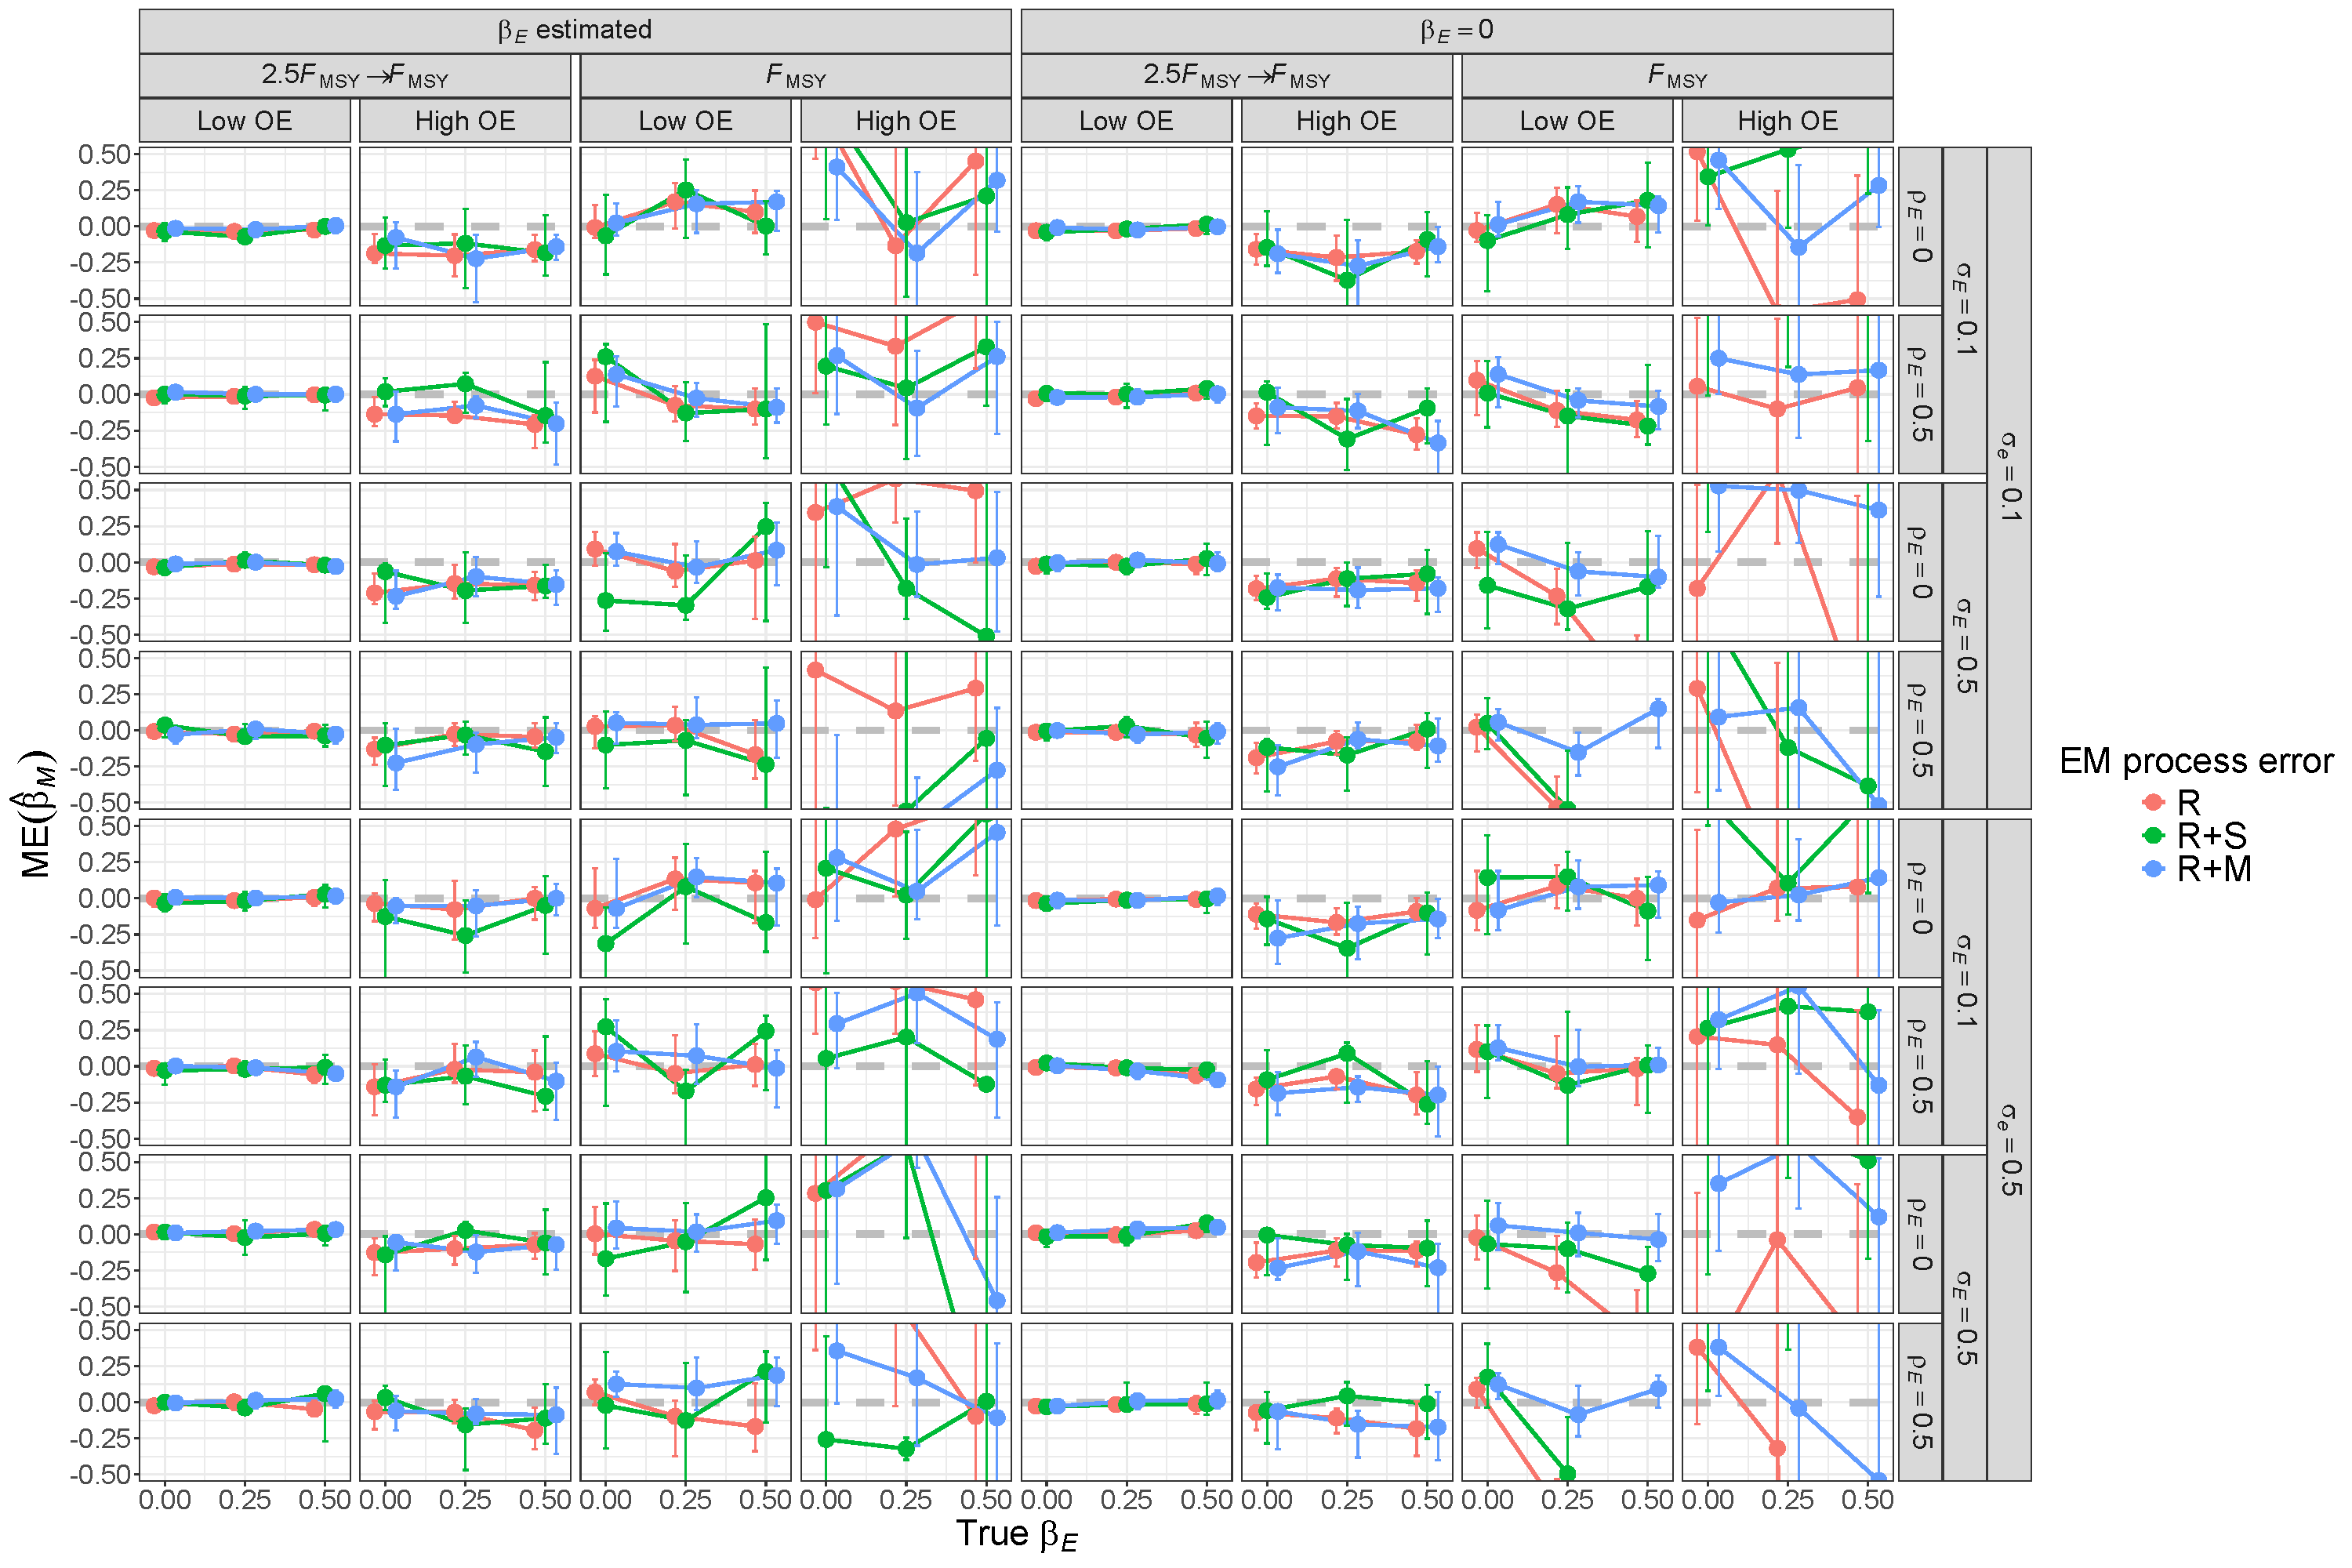
\includegraphics[height = \textheight]{beta_M_bias_Rom}
\end{center}
\caption{For R OMs, median error (ME) of estimates of $\beta_M$ from fitting EMs with alternative process error assumptions and treatment of covariate effect ($\beta_E = 0$ or estimated). Vertical lines represent 95\% confidence intervals.}\label{beta_M_bias_Rom}
\end{figure}
\end{landscape}

\begin{landscape}
\begin{figure}
\begin{center}
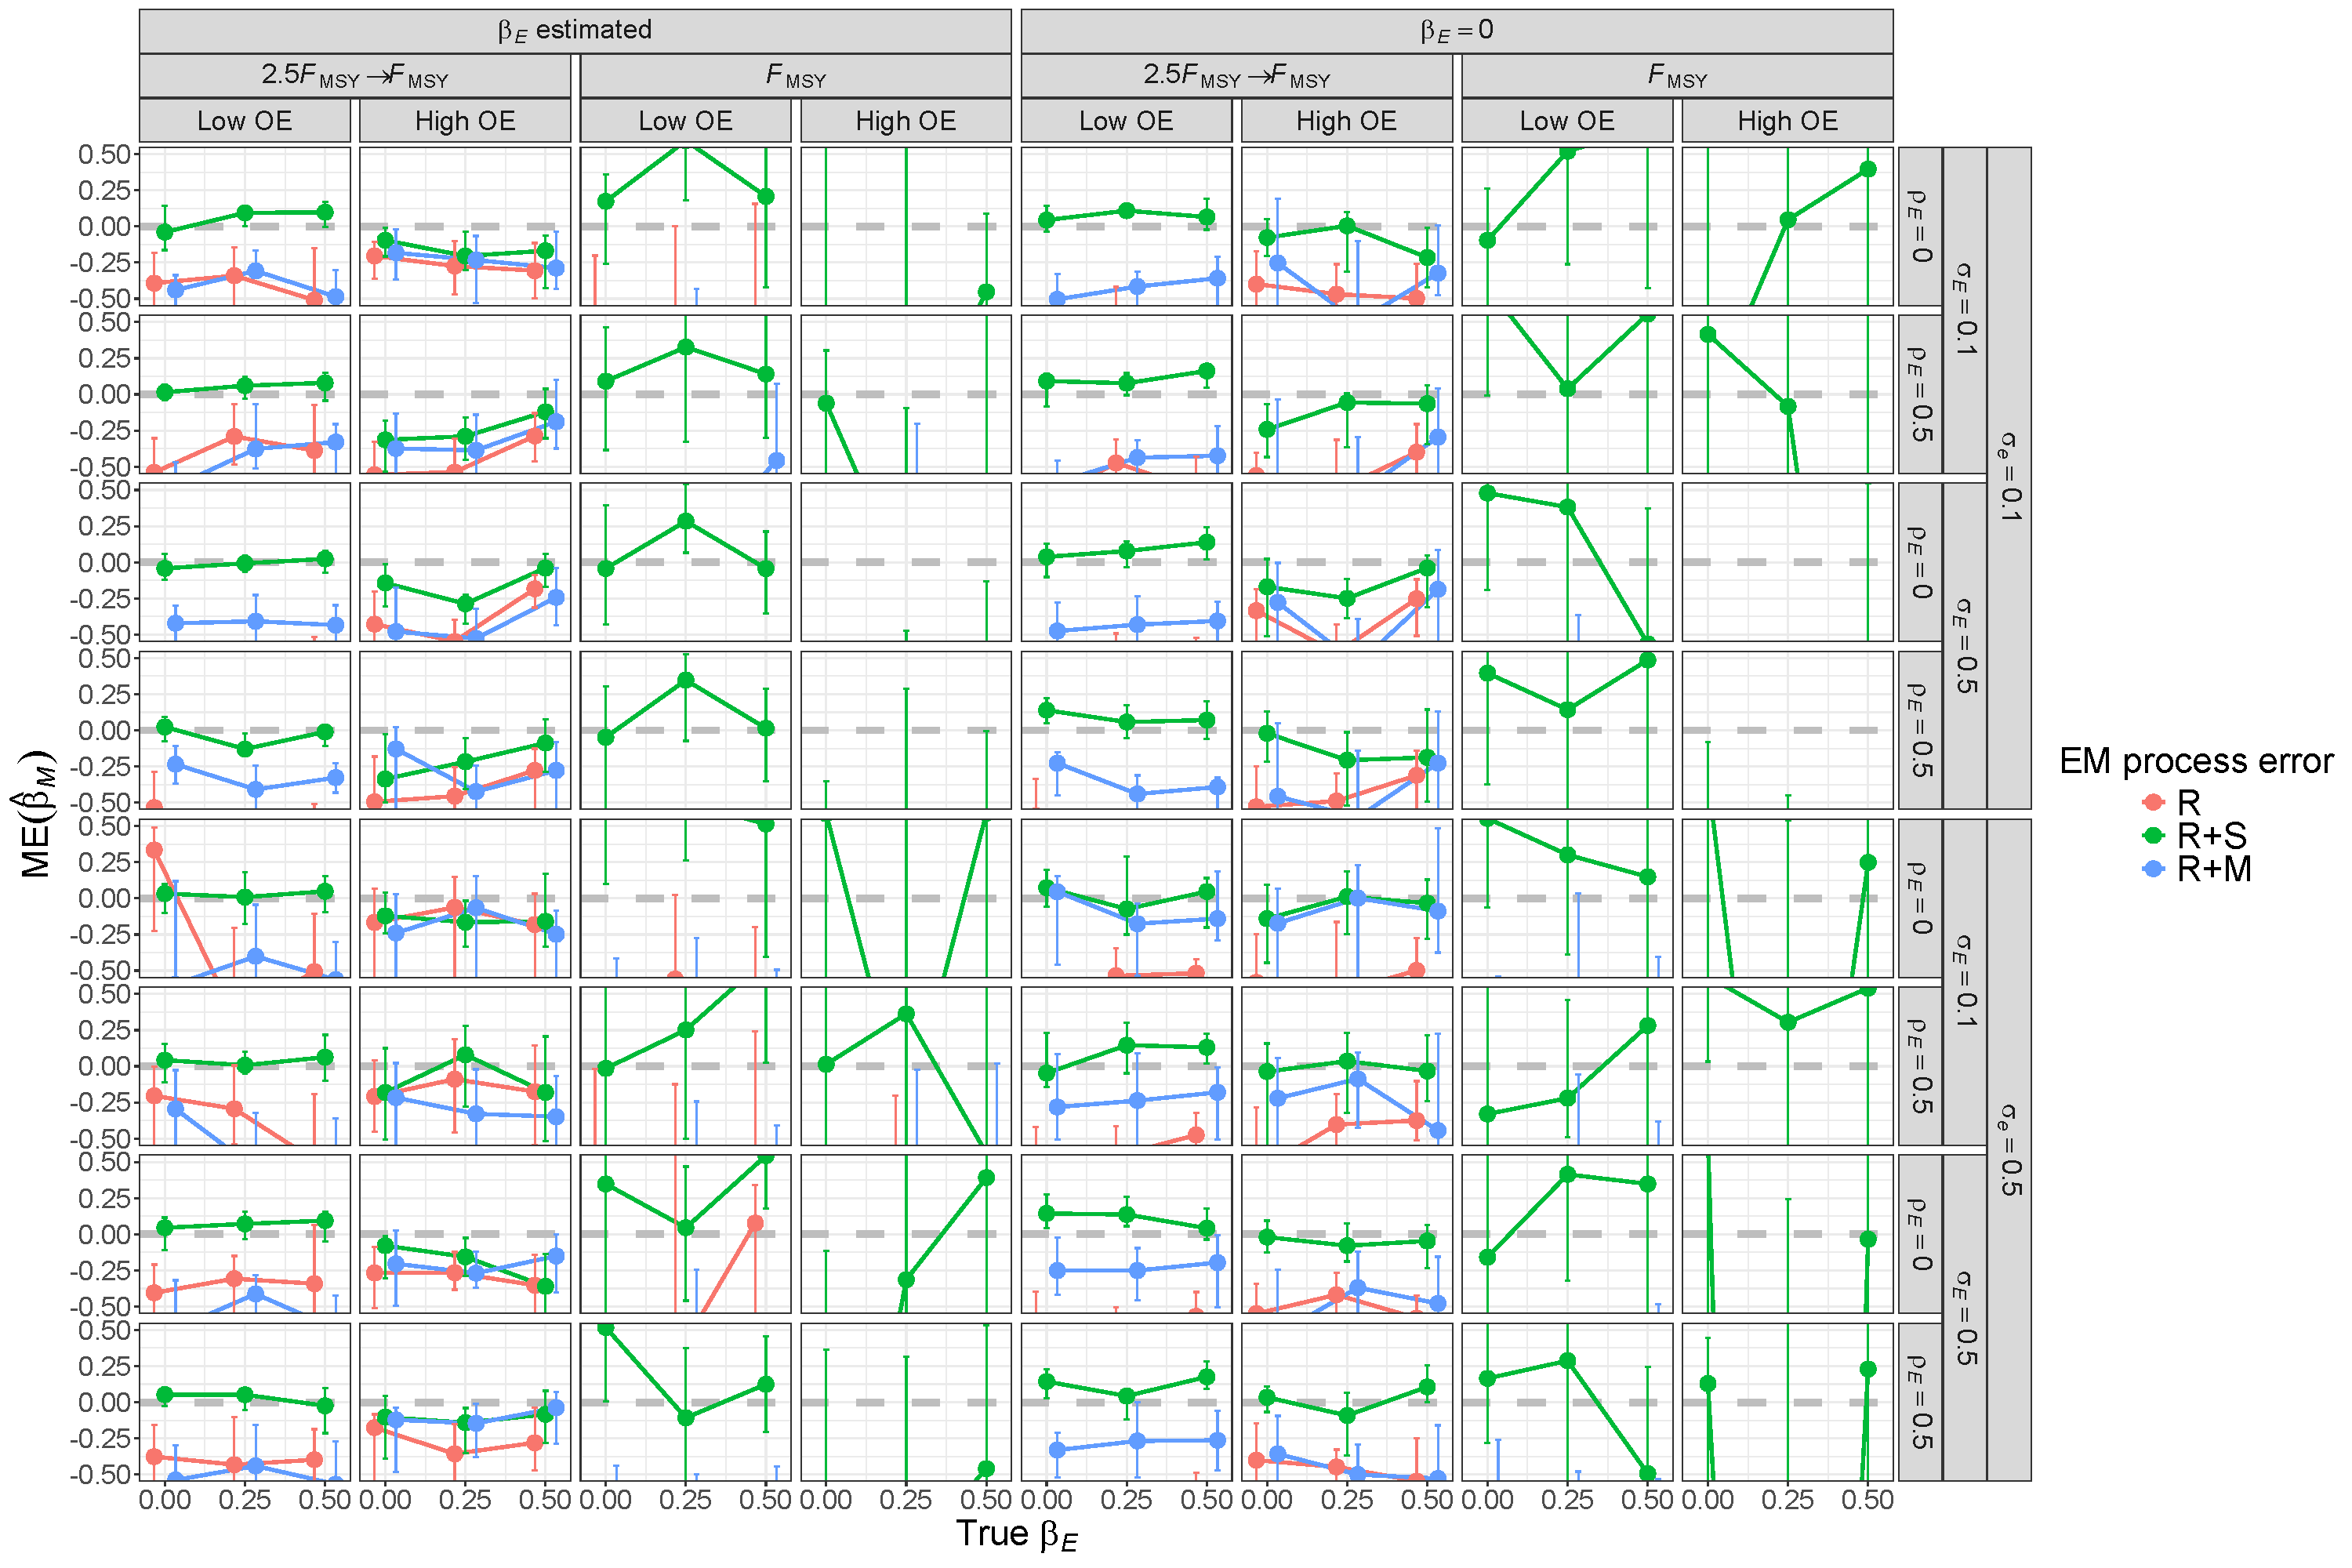
\includegraphics[height = \textheight]{beta_M_bias_RSom}
\end{center}
\caption{For R+S OMs, median error (ME) of estimates of $\beta_M$ from fitting EMs with alternative process error assumptions and treatment of covariate effect ($\beta_E = 0$ or estimated). Vertical lines represent 95\% confidence intervals.}\label{beta_M_bias_RSom}
\end{figure}
\end{landscape}

\begin{landscape}
\begin{figure}
\begin{center}
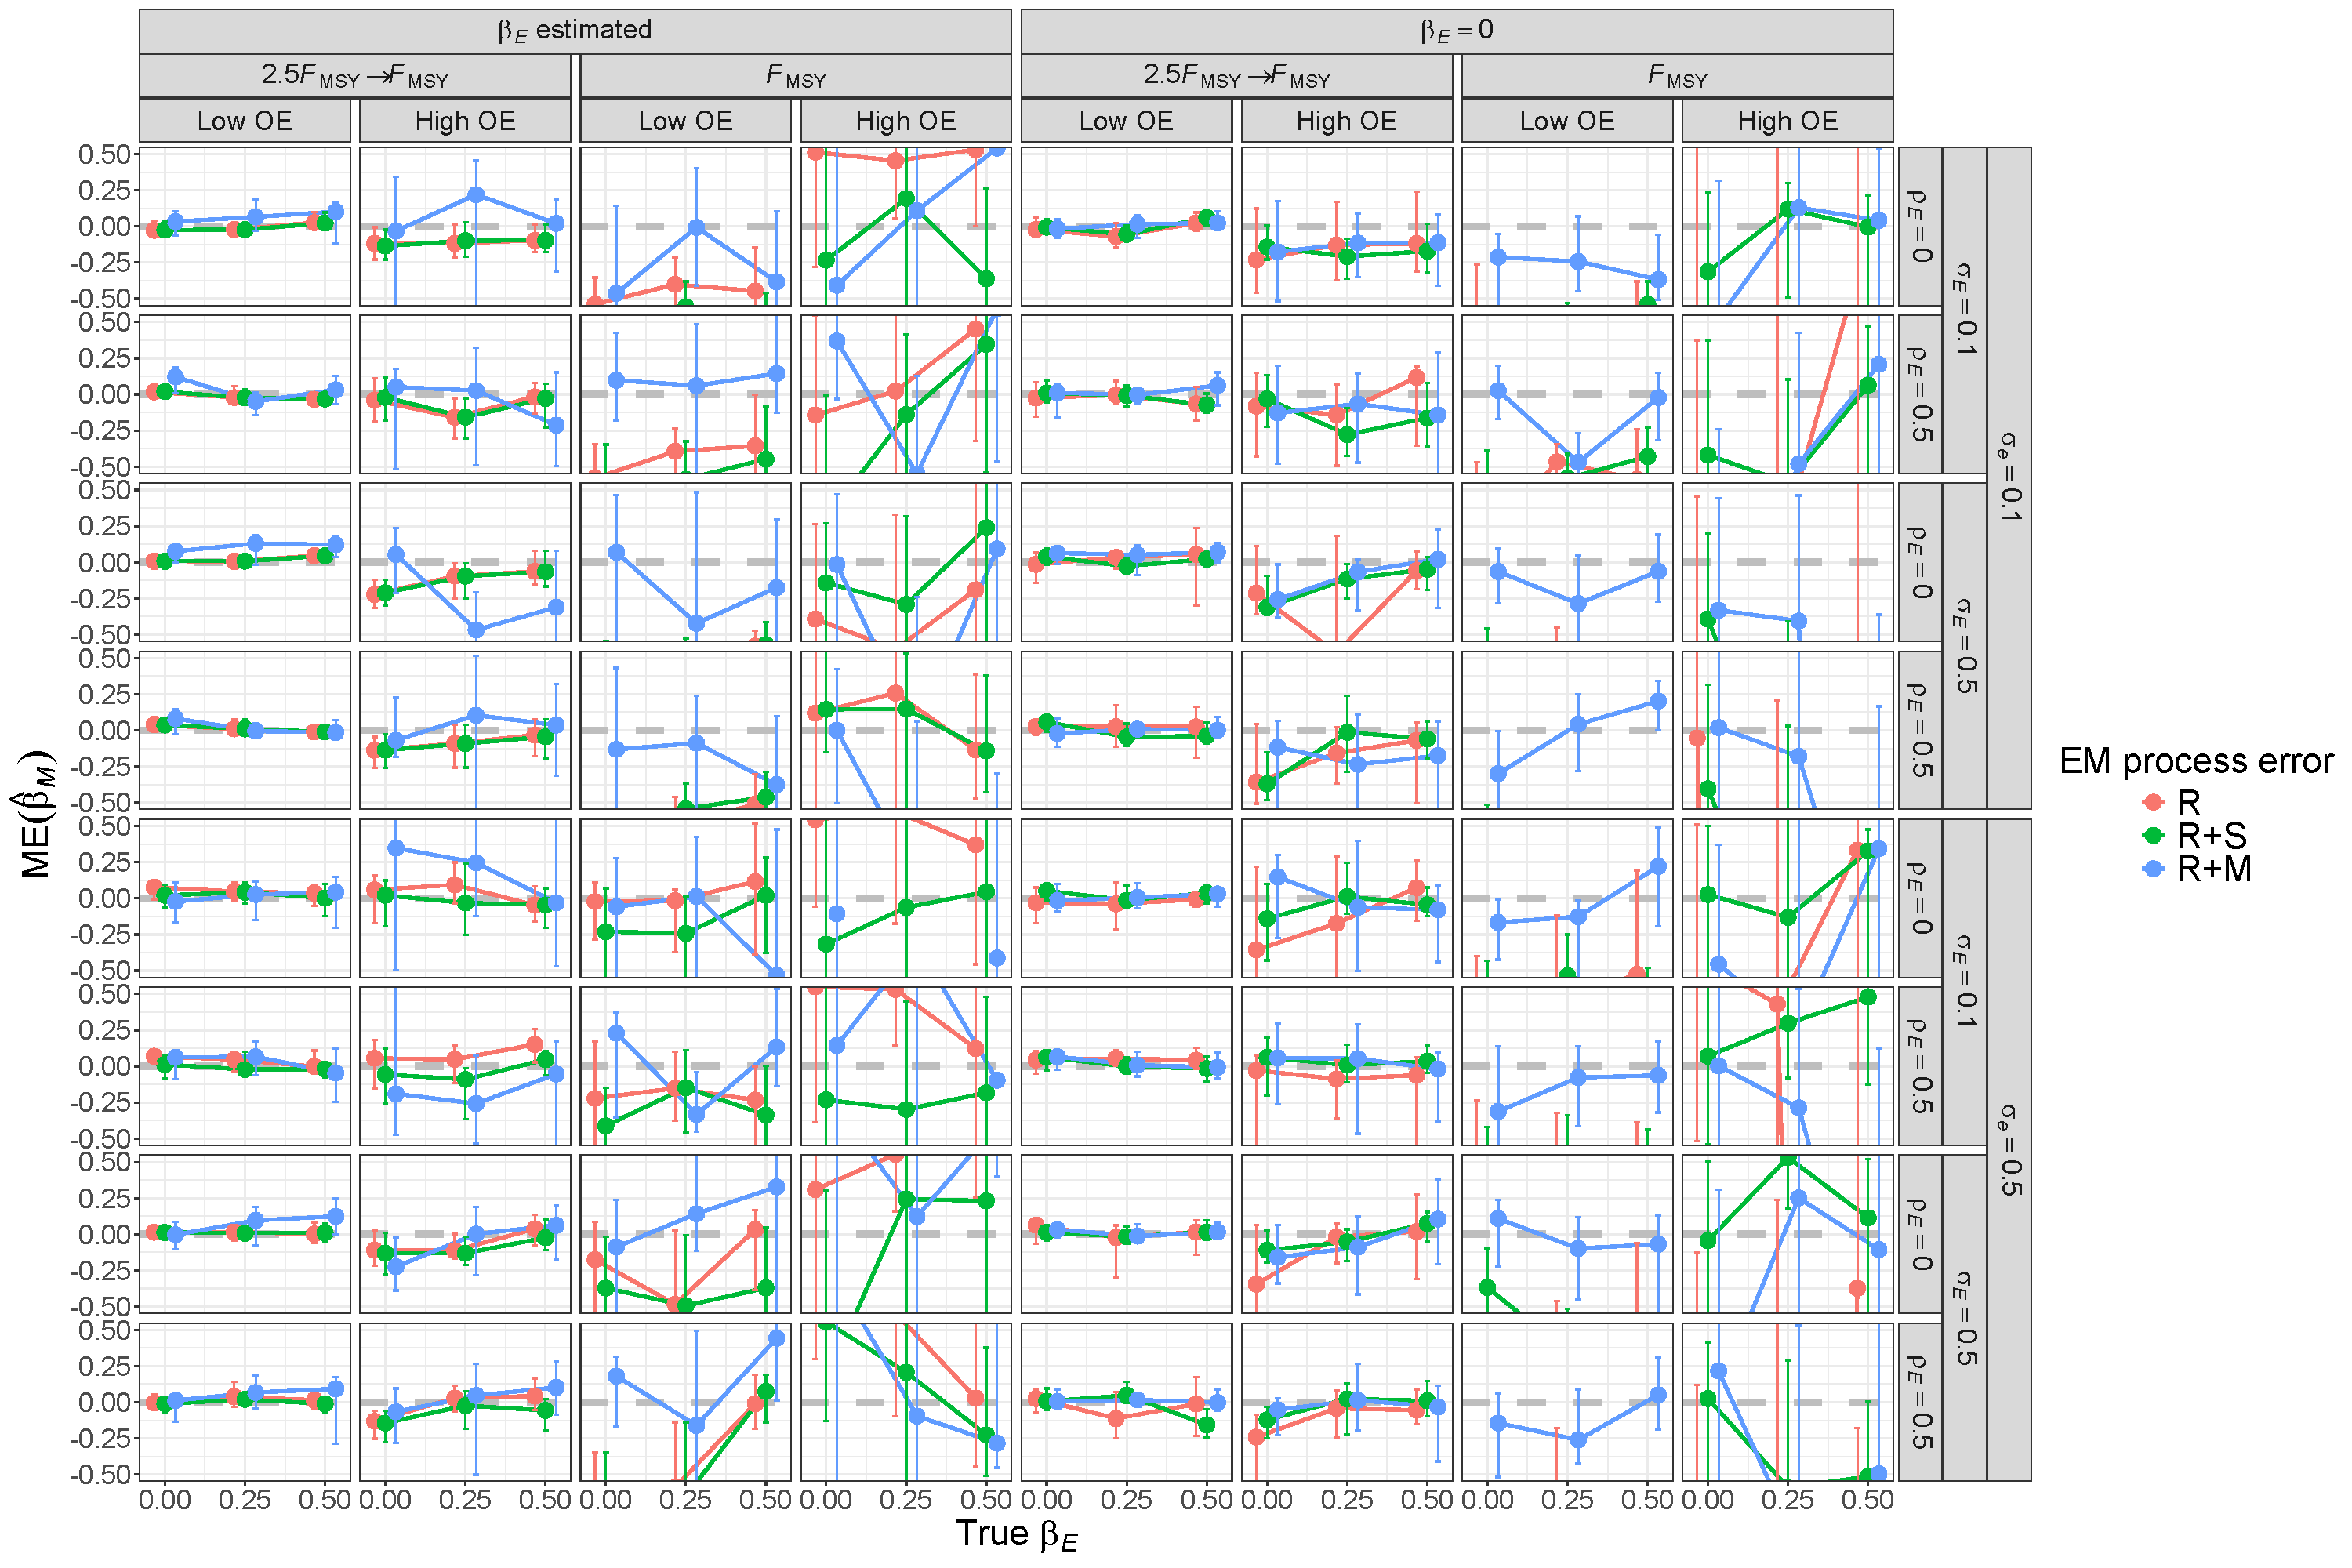
\includegraphics[height = \textheight]{beta_M_bias_RMom}
\end{center}
\caption{For R+M OMs, median error (ME) of estimates of $\beta_M$ from fitting EMs with alternative process error assumptions and treatment of covariate effect ($\beta_E = 0$ or estimated). Vertical lines represent 95\% confidence intervals.}\label{beta_M_bias_RMom}
\end{figure}
\end{landscape}

\DIFdelbegin %DIFDELCMD < \hypertarget{median-natural-mortality-parameter-standard-error-estimation-bias}{%
%DIFDELCMD < \subsection*{Median natural mortality parameter standard error estimation bias}\label{median-natural-mortality-parameter-standard-error-estimation-bias}}
%DIFDELCMD < %%%
\DIFdelend \DIFaddbegin \subsection*{\DIFadd{Median natural mortality parameter standard error estimation bias}}\label{median-natural-mortality-parameter-standard-error-estimation-bias}
\DIFaddend \addcontentsline{toc}{subsection}{Median natural mortality parameter standard error estimation bias}

\begin{landscape}
\begin{figure}
\begin{center}
\DIFdelbeginFL %DIFDELCMD < 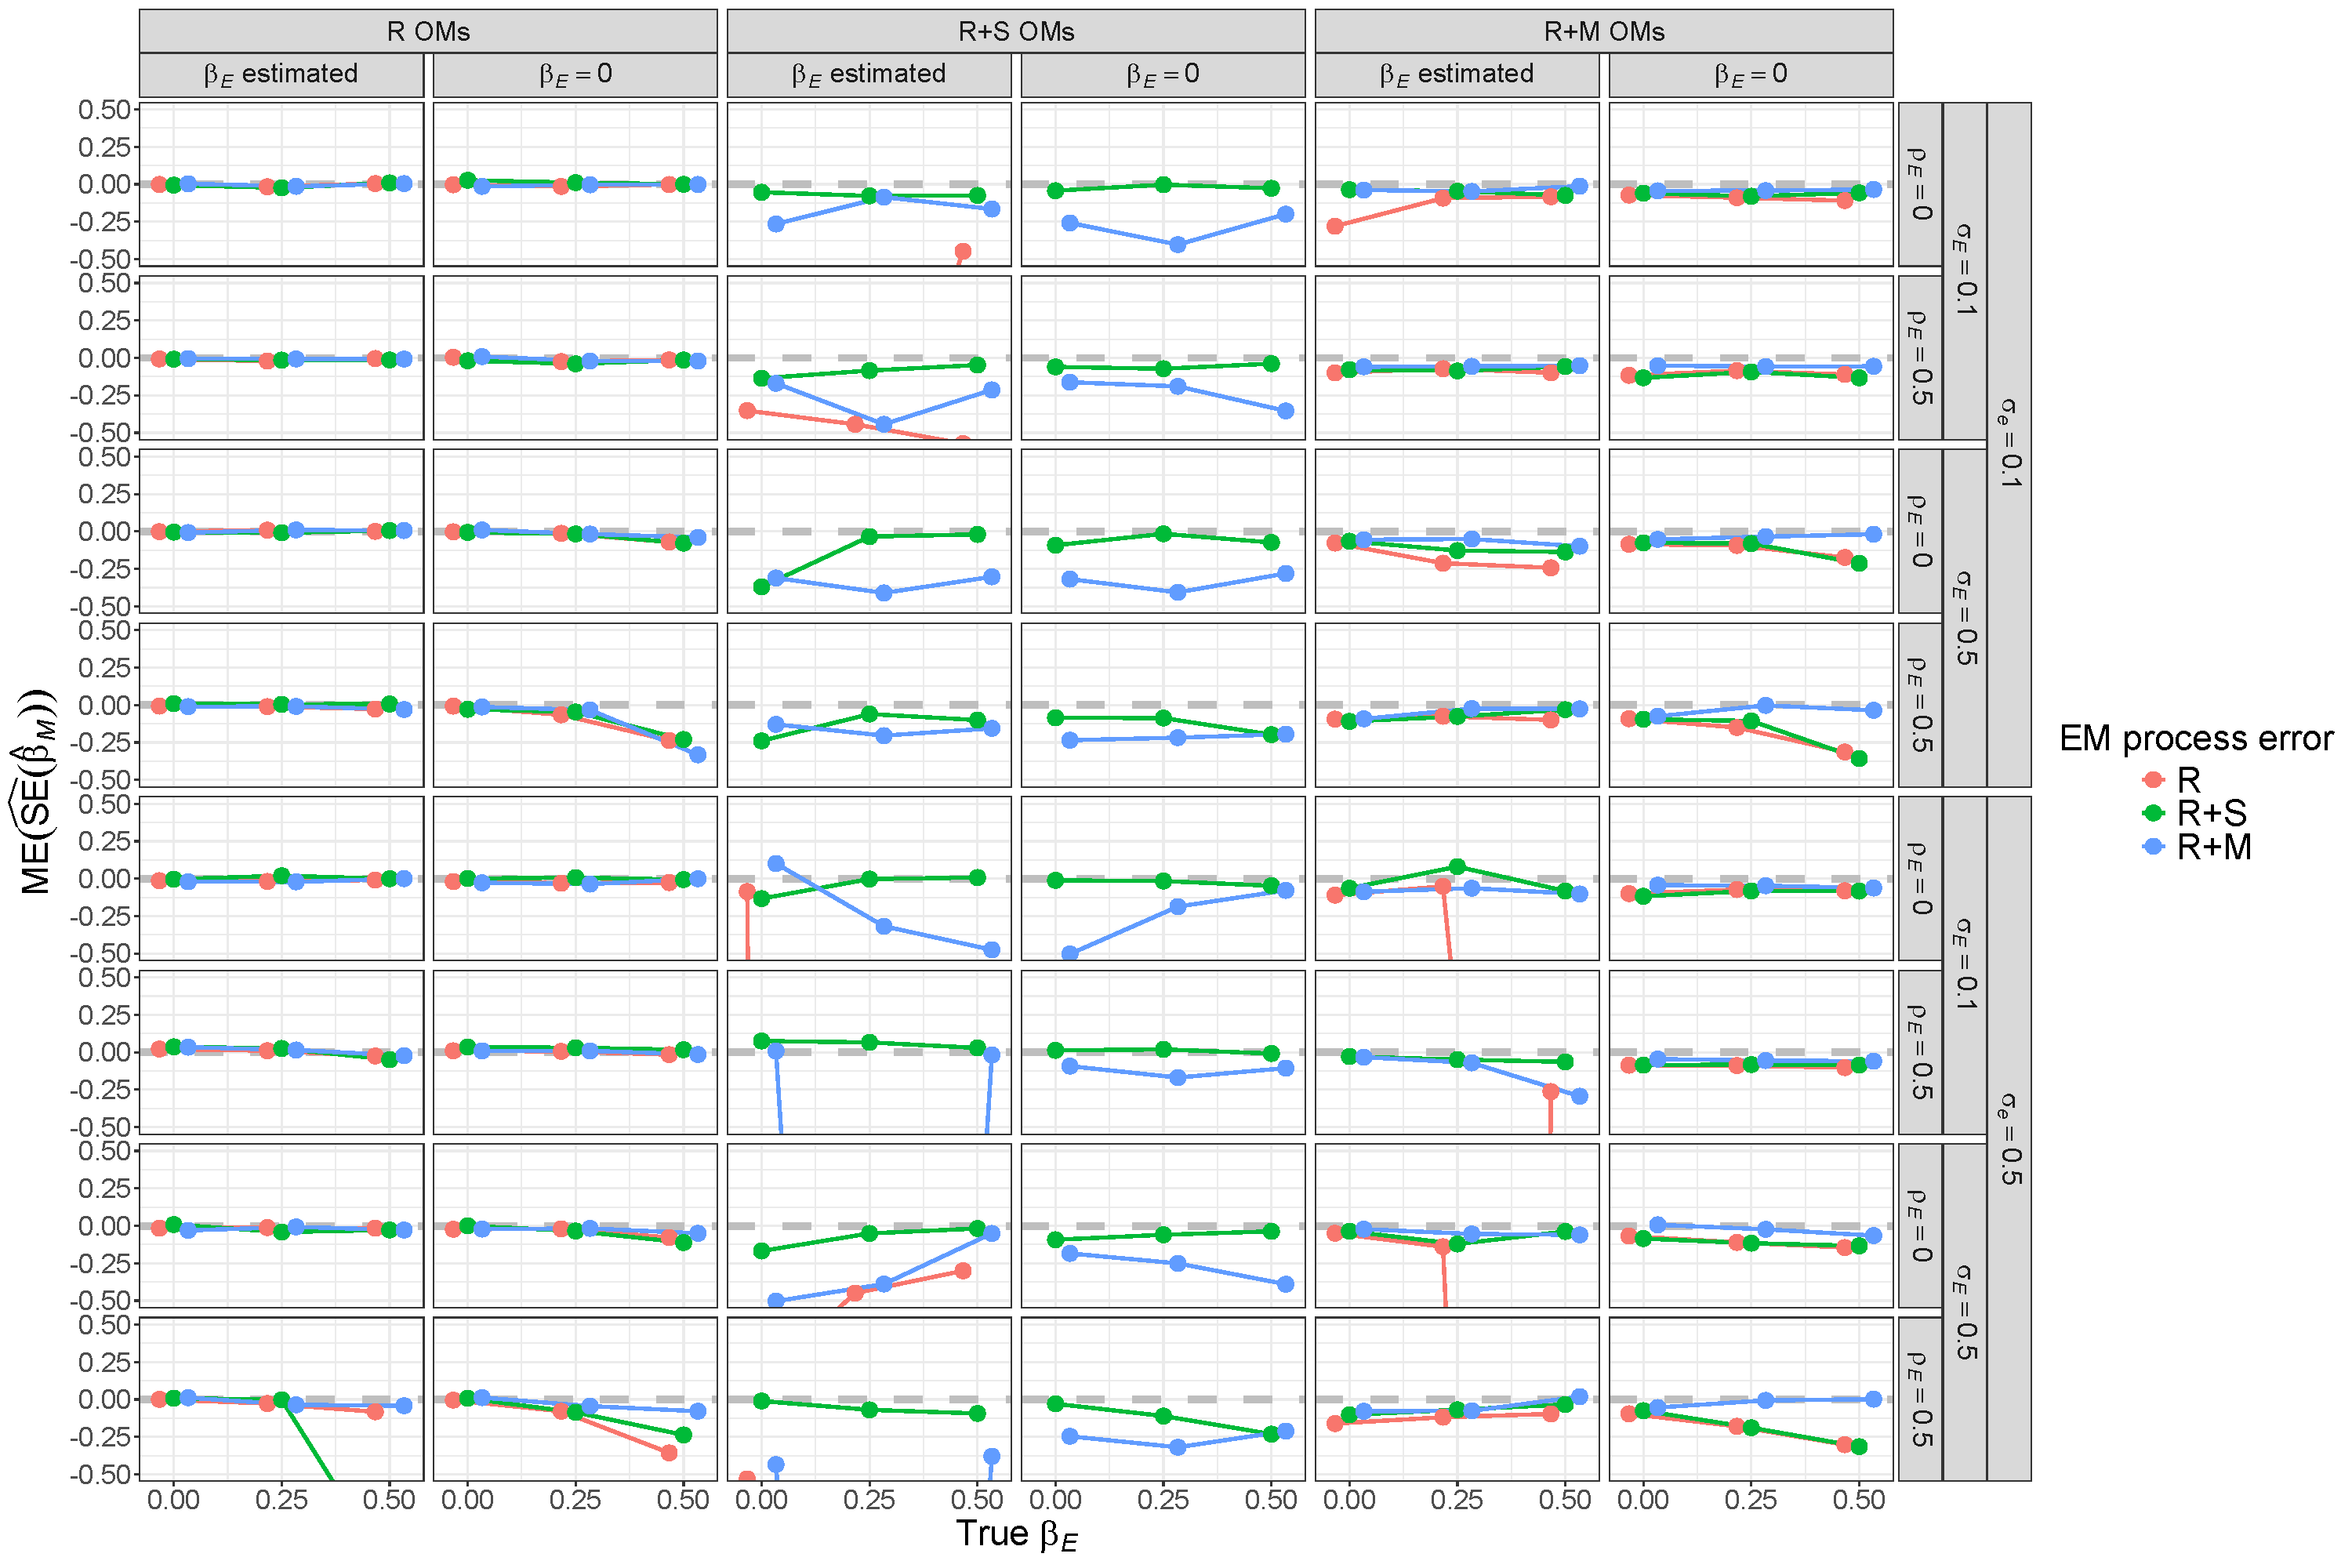
\includegraphics[height = \textheight]{se_beta_M_bias_main}
%DIFDELCMD < \end{center}
%DIFDELCMD < %%%
%DIFDELCMD < \caption{%
{%DIFAUXCMD
\DIFdelFL{Median error (ME) of Hessian-based estimates of standard error for median natural mortality parameter $\beta_M$ from fitting EMs with alternative process error assumptions and treatment of the covariate effect ($\beta_ E= 0$ or estimated). All OMs had low observation error and contrast in fishing mortality. True standard error is defined as the mean of the standard error estimates accross converged fits to simulated data sets for a given OM scenario.}}%DIFAUXCMD
%DIFDELCMD < \label{se_beta_M_bias}
%DIFDELCMD < \end{figure}
%DIFDELCMD < \end{landscape}
%DIFDELCMD < 

%DIFDELCMD < \begin{landscape}
%DIFDELCMD < \begin{figure}
%DIFDELCMD < \begin{center}
%DIFDELCMD < %%%
\DIFdelendFL 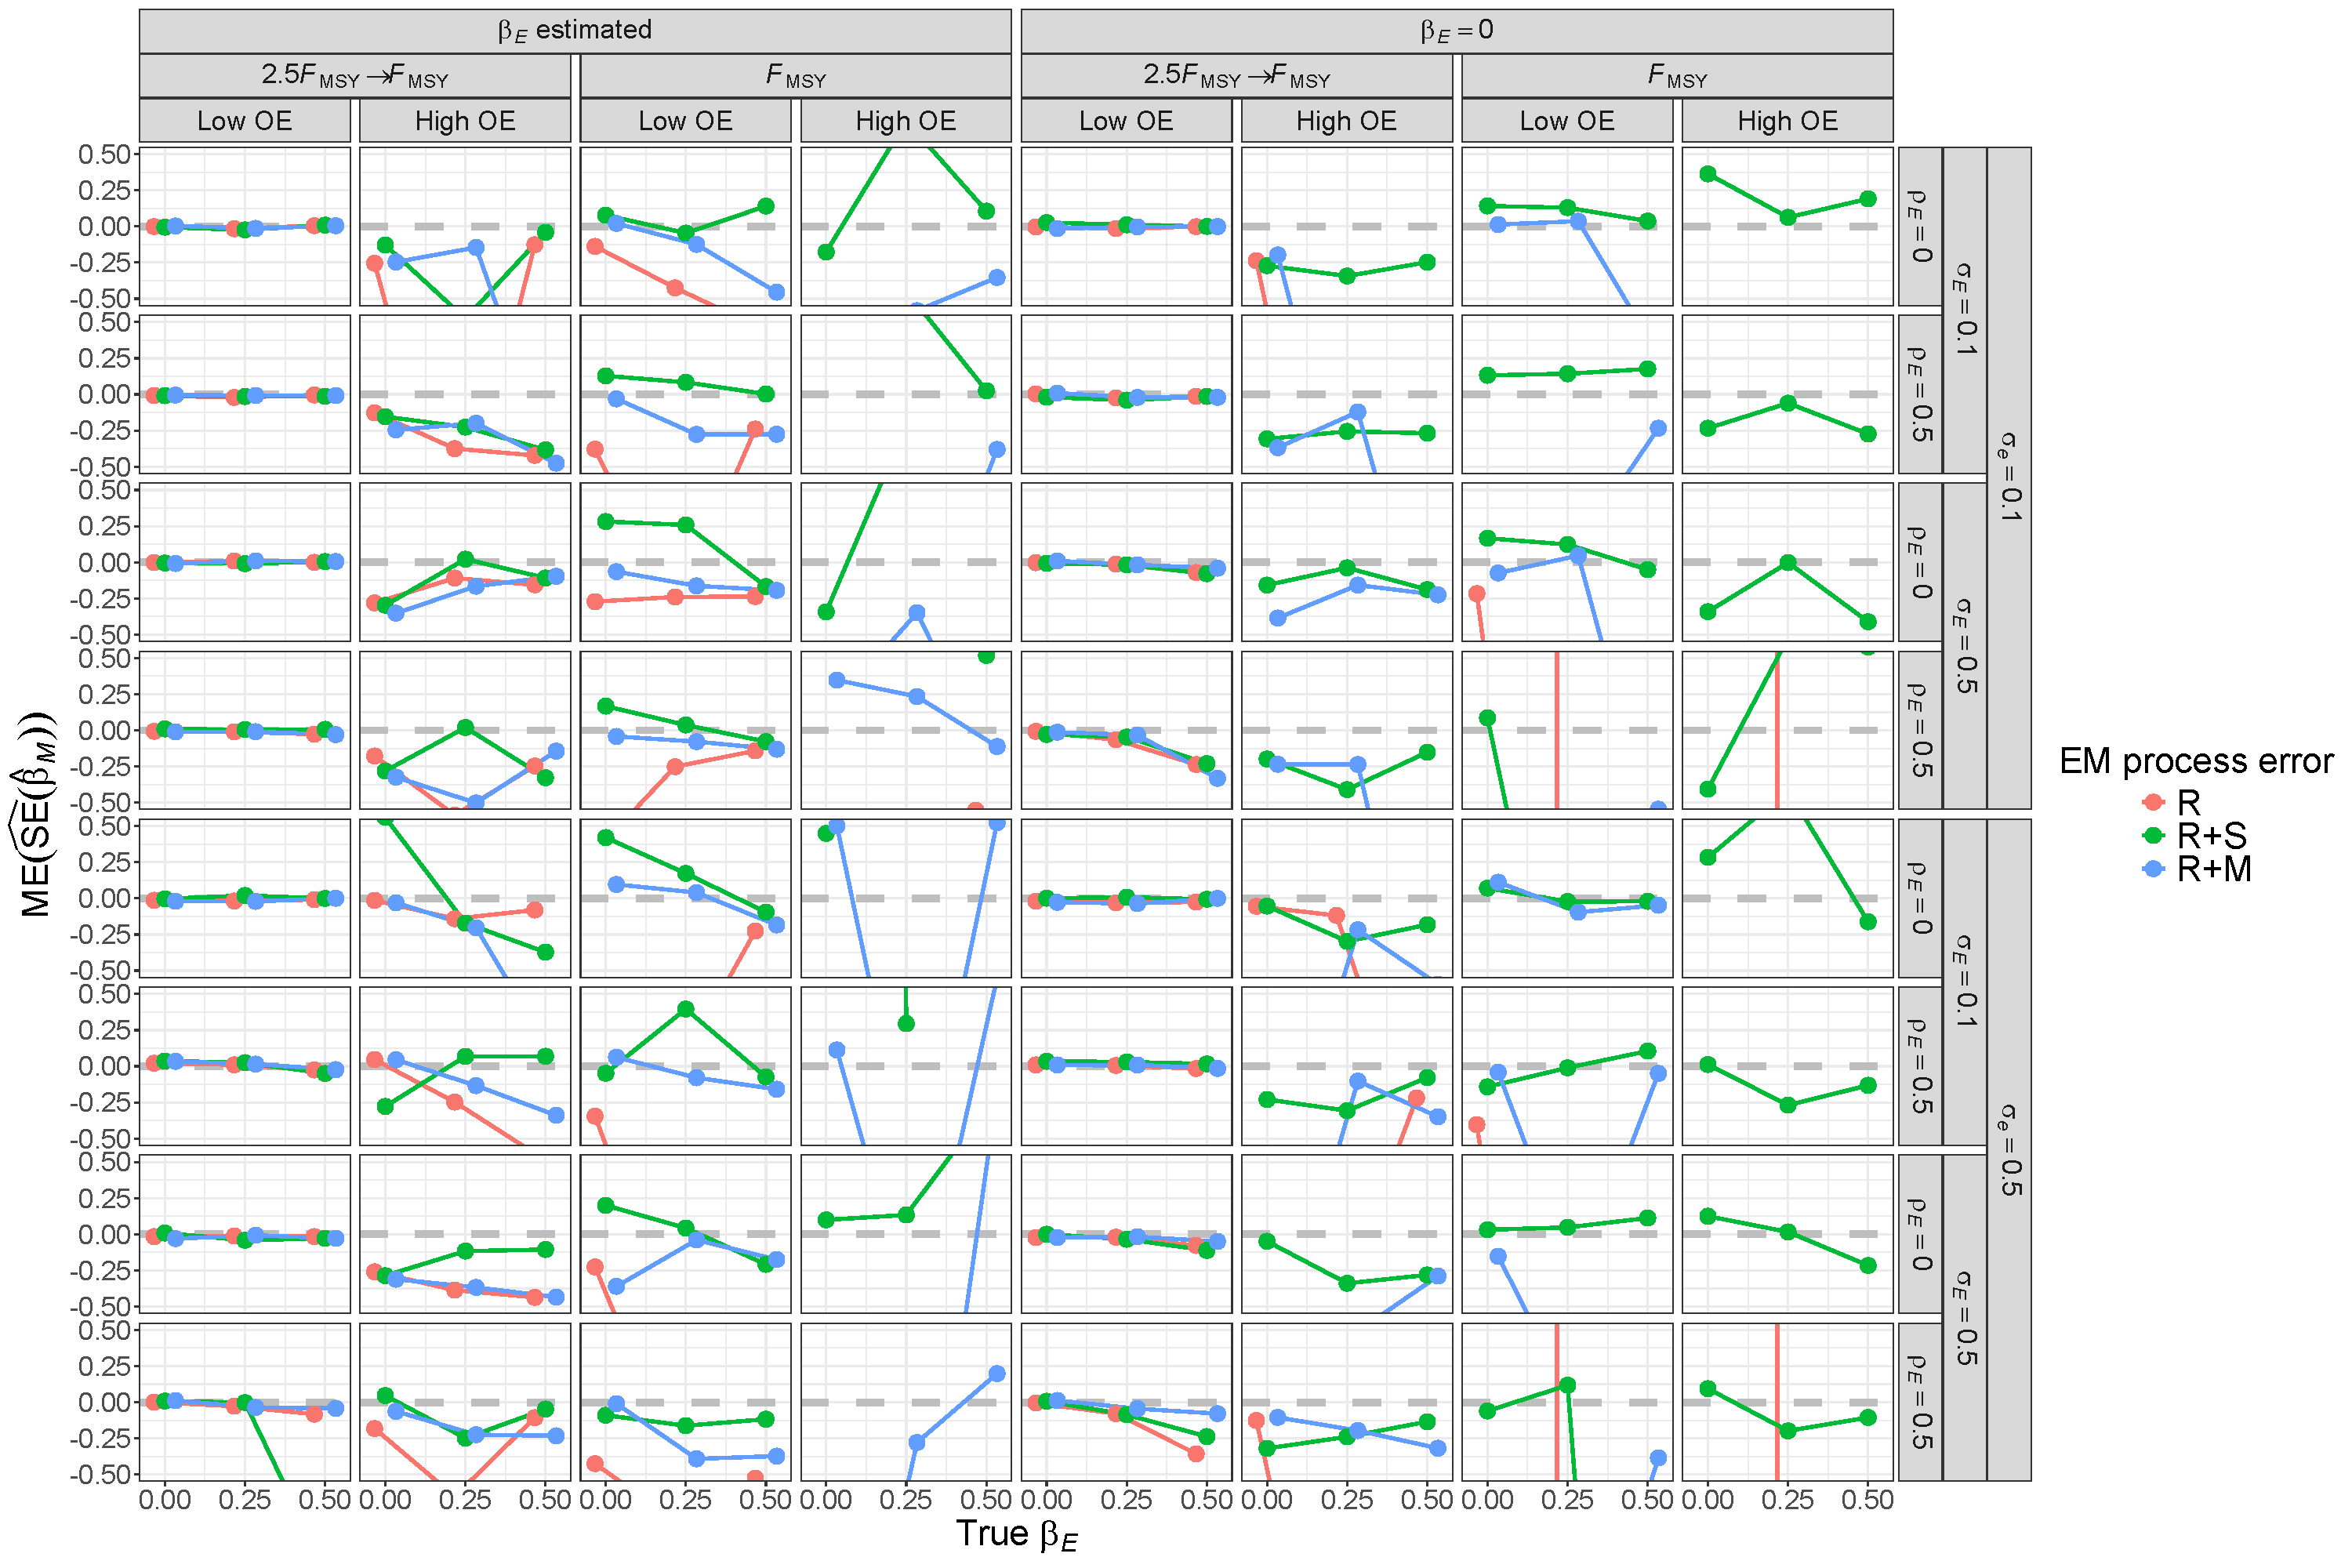
\includegraphics[height = \textheight]{se_beta_M_bias_Rom}
\end{center}
\caption{For R OMs, median error (ME) of Hessian-based estimates of standard error for median \DIFdelbeginFL \DIFdelFL{natural mortality }\DIFdelendFL \DIFaddbeginFL \DIFaddFL{$M$ }\DIFaddendFL parameter \DIFaddbeginFL \DIFaddFL{(}\DIFaddendFL $\beta_M$\DIFaddbeginFL \DIFaddFL{) }\DIFaddendFL from fitting EMs with alternative process error assumptions and treatment of the covariate effect ($\beta_ E= 0$ or estimated). True standard error is defined as the mean of the standard error estimates accross converged fits to simulated data sets for a given OM scenario.}\label{se_beta_M_bias_Rom}
\end{figure}
\end{landscape}

\begin{landscape}
\begin{figure}
\begin{center}
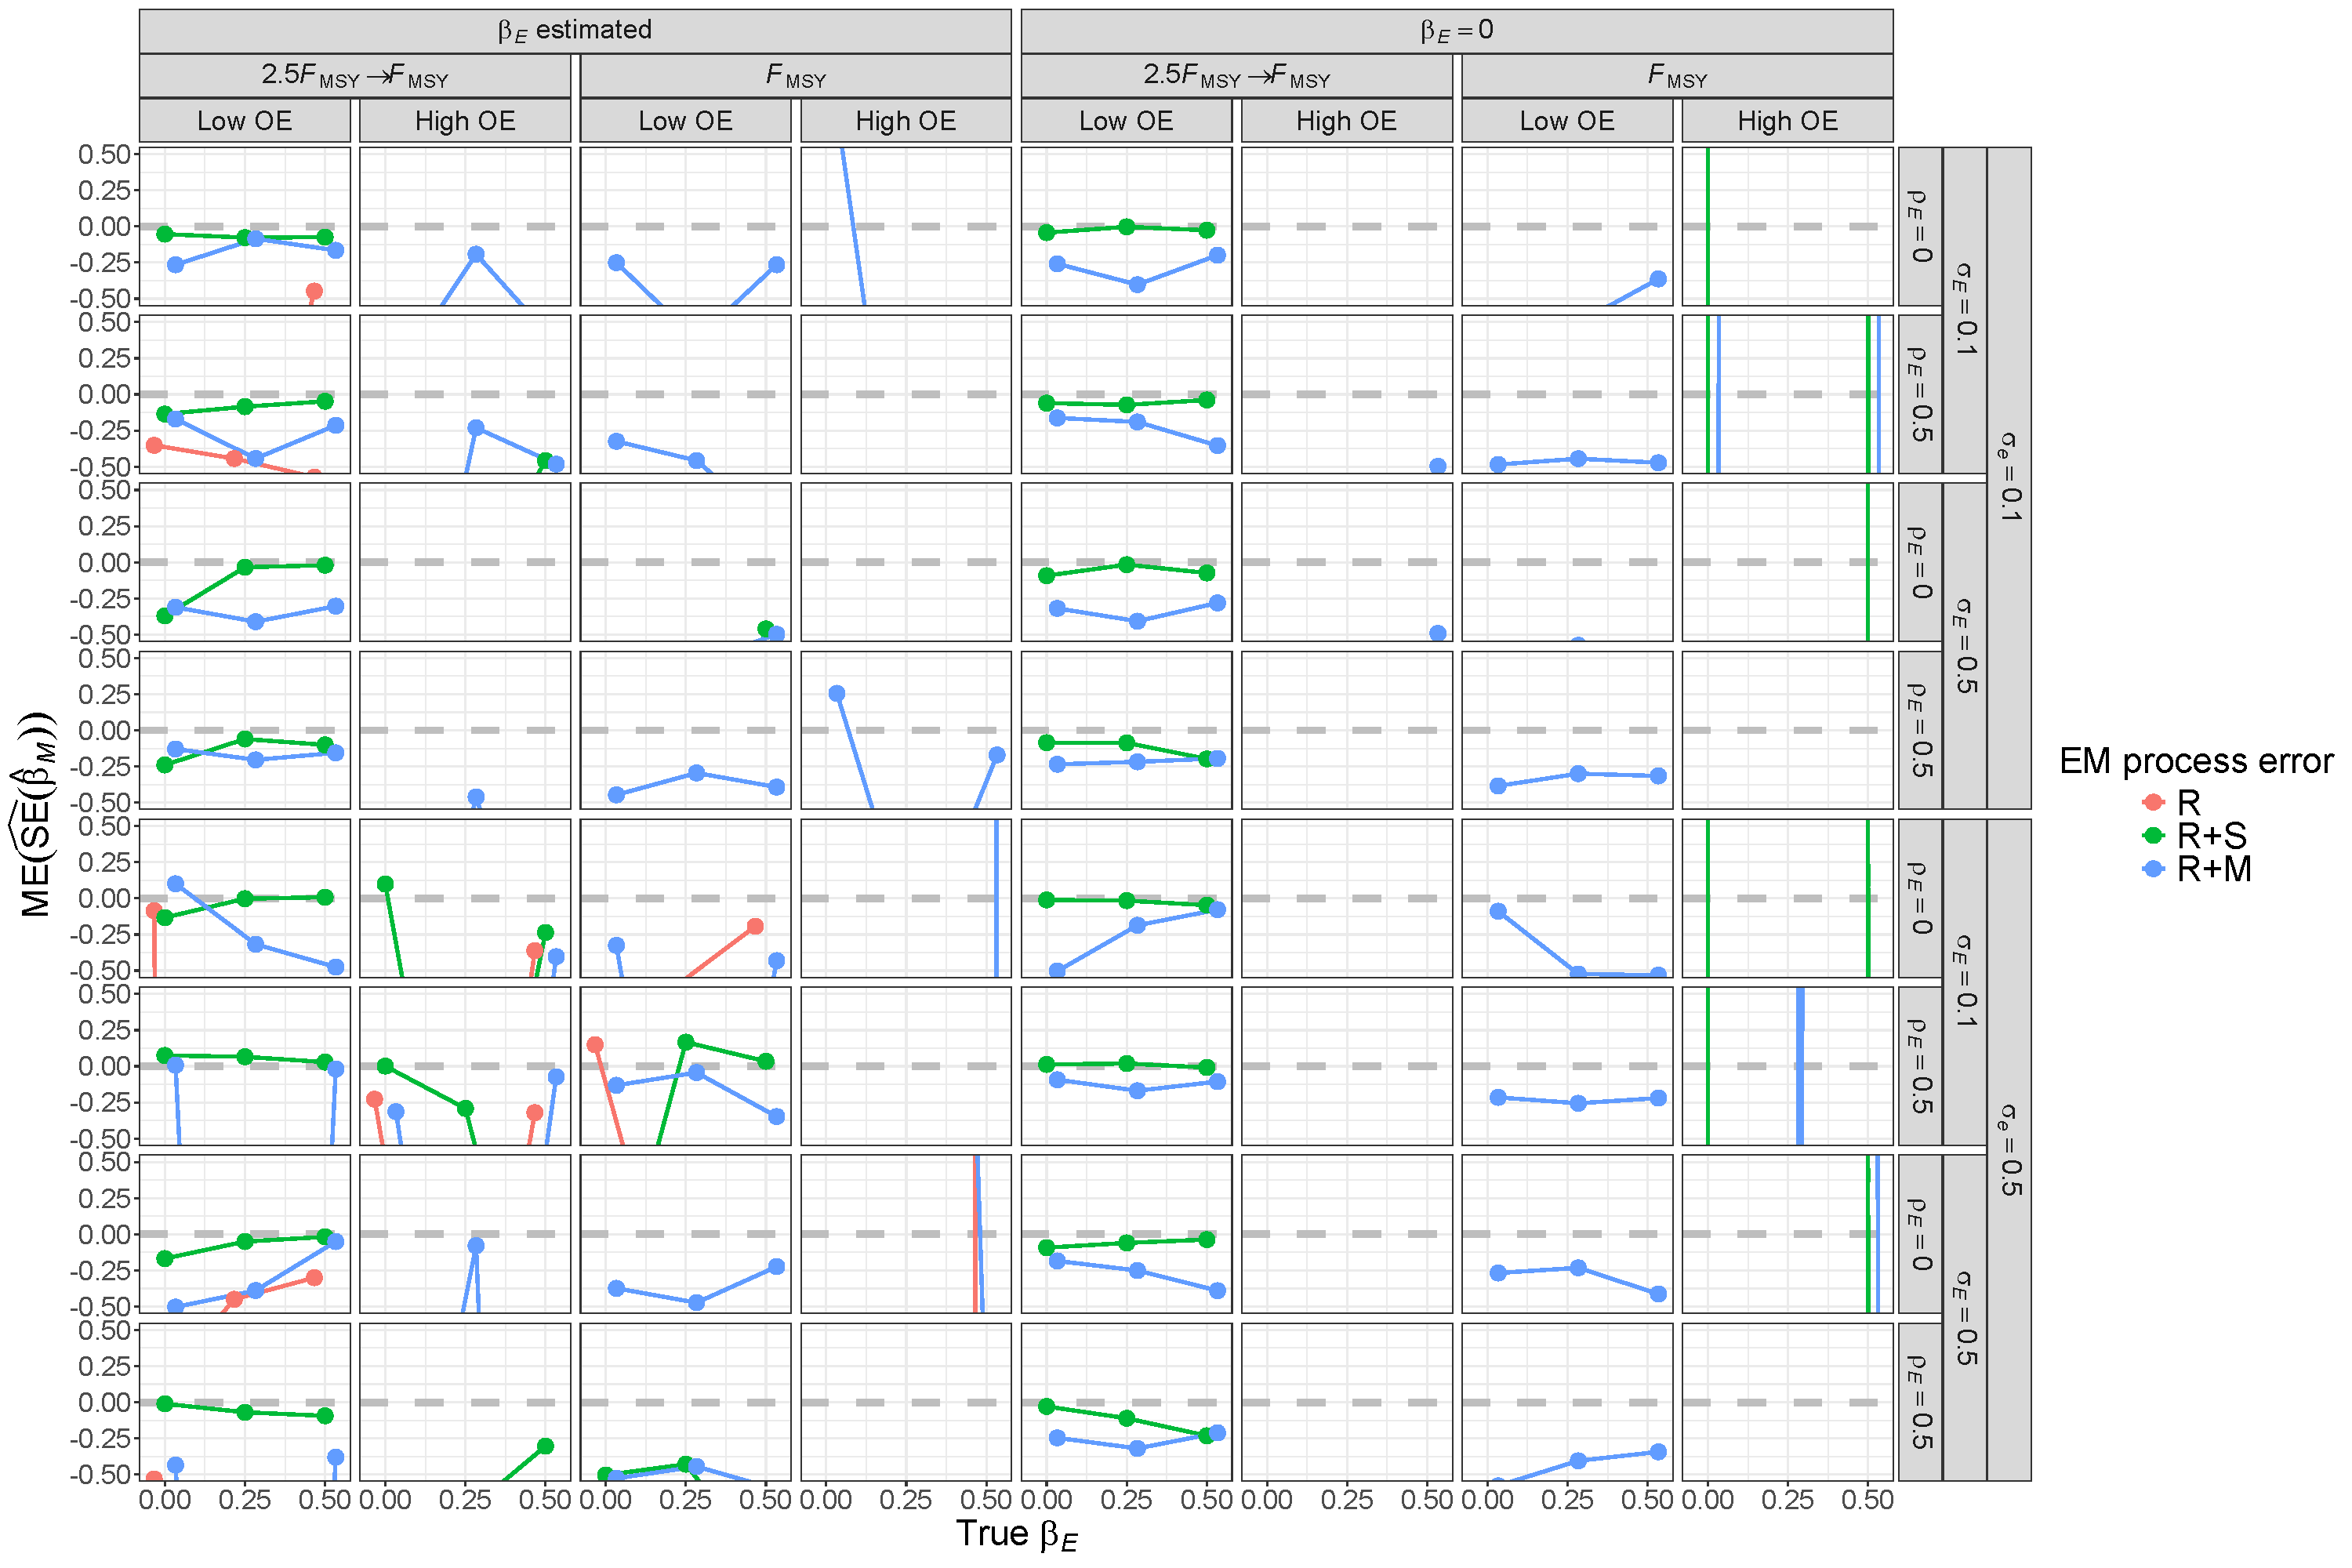
\includegraphics[height = \textheight]{se_beta_M_bias_RSom}
\end{center}
\caption{For R+S OMs, median error (ME) of Hessian-based estimates of standard error for median \DIFdelbeginFL \DIFdelFL{natural mortality }\DIFdelendFL \DIFaddbeginFL \DIFaddFL{$M$ }\DIFaddendFL parameter \DIFaddbeginFL \DIFaddFL{(}\DIFaddendFL $\beta_M$\DIFaddbeginFL \DIFaddFL{) }\DIFaddendFL from fitting EMs with alternative process error assumptions and treatment of the covariate effect ($\beta_ E= 0$ or estimated). True standard error is defined as the mean of the standard error estimates accross converged fits to simulated data sets for a given OM scenario.}\label{se_beta_M_bias_RSom}
\end{figure}
\end{landscape}

\begin{landscape}
\begin{figure}
\begin{center}
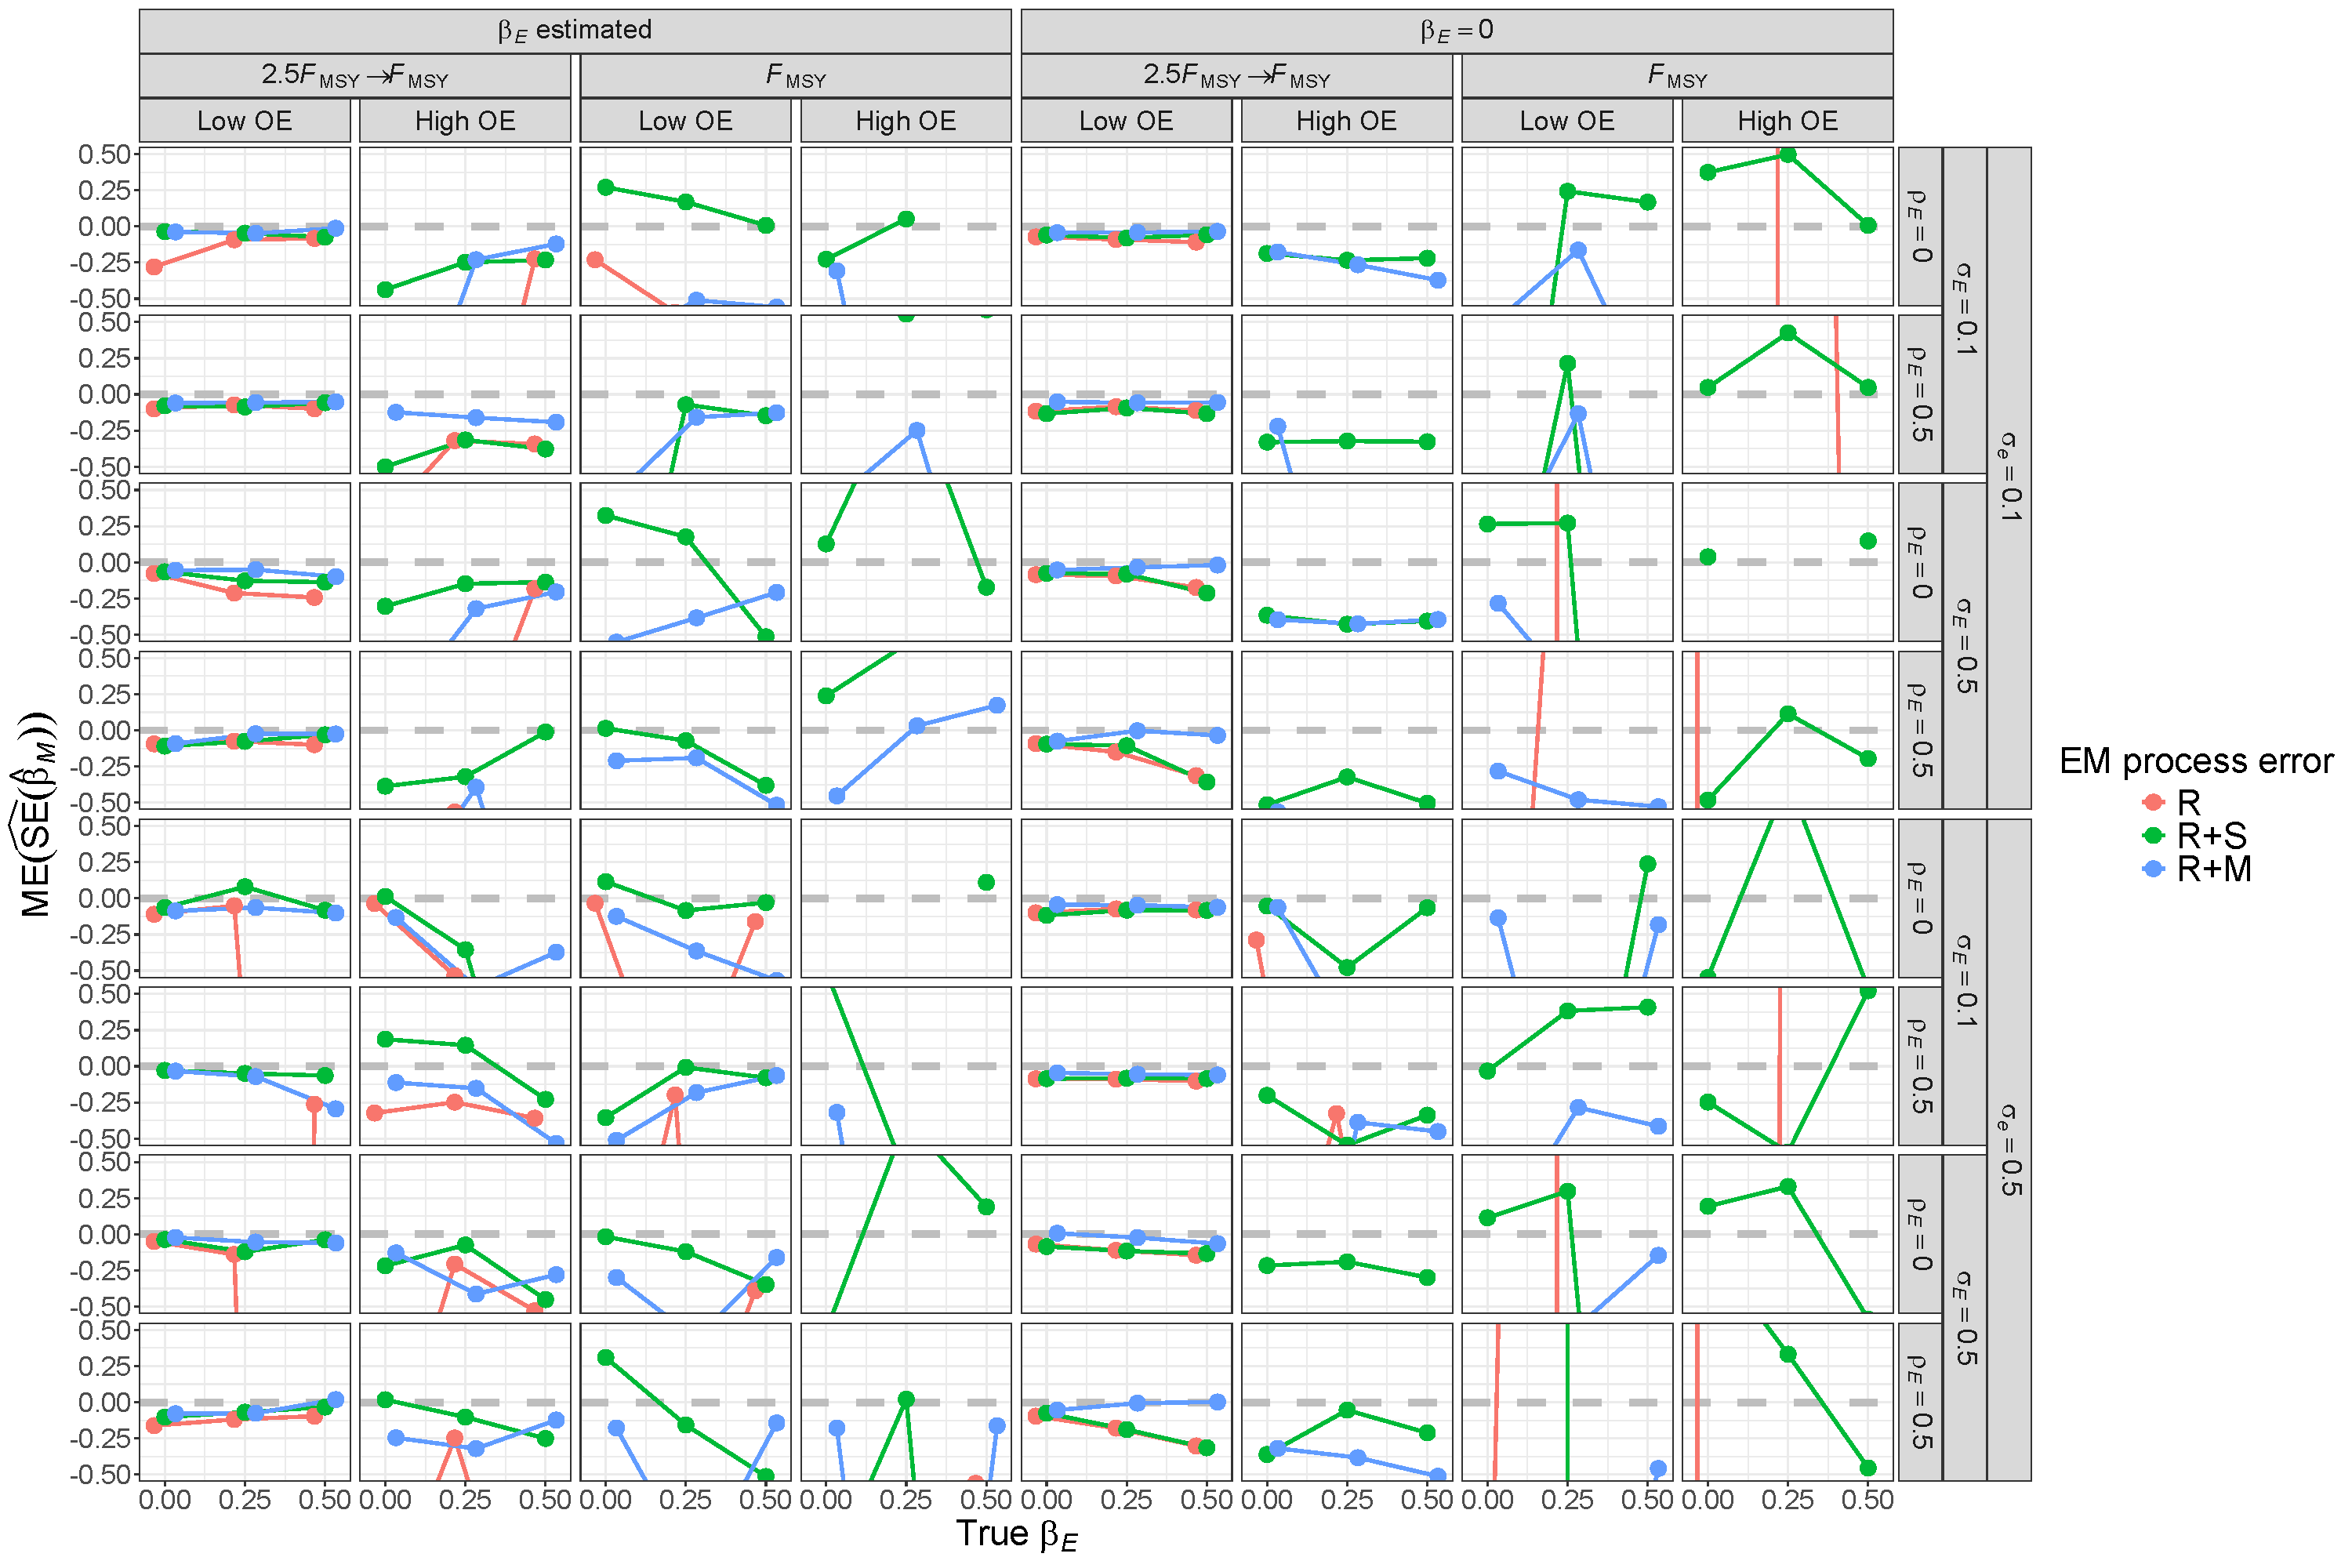
\includegraphics[height = \textheight]{se_beta_M_bias_RMom}
\end{center}
\caption{For R+M OMs, median error (ME) of Hessian-based estimates of standard error for median \DIFdelbeginFL \DIFdelFL{natural mortality }\DIFdelendFL \DIFaddbeginFL \DIFaddFL{$M$ }\DIFaddendFL parameter \DIFaddbeginFL \DIFaddFL{(}\DIFaddendFL $\beta_M$\DIFaddbeginFL \DIFaddFL{) }\DIFaddendFL from fitting EMs with alternative process error assumptions and treatment of the covariate effect ($\beta_ E= 0$ or estimated). True standard error is defined as the mean of the standard error estimates accross converged fits to simulated data sets for a given OM scenario.}\label{se_beta_M_bias_RMom}
\end{figure}
\end{landscape}

\DIFdelbegin %DIFDELCMD < \hypertarget{median-natural-mortality-parameter-confidence-interval-coverage}{%
%DIFDELCMD < \subsection*{Median Natural mortality parameter confidence interval coverage}\label{median-natural-mortality-parameter-confidence-interval-coverage}}
%DIFDELCMD < %%%
\DIFdelend \DIFaddbegin \subsection*{\DIFadd{Median Natural mortality parameter confidence interval coverage}}\label{median-natural-mortality-parameter-confidence-interval-coverage}
\DIFaddend \addcontentsline{toc}{subsection}{Median Natural mortality parameter confidence interval coverage}

\begin{landscape}
\begin{figure}
\begin{center}
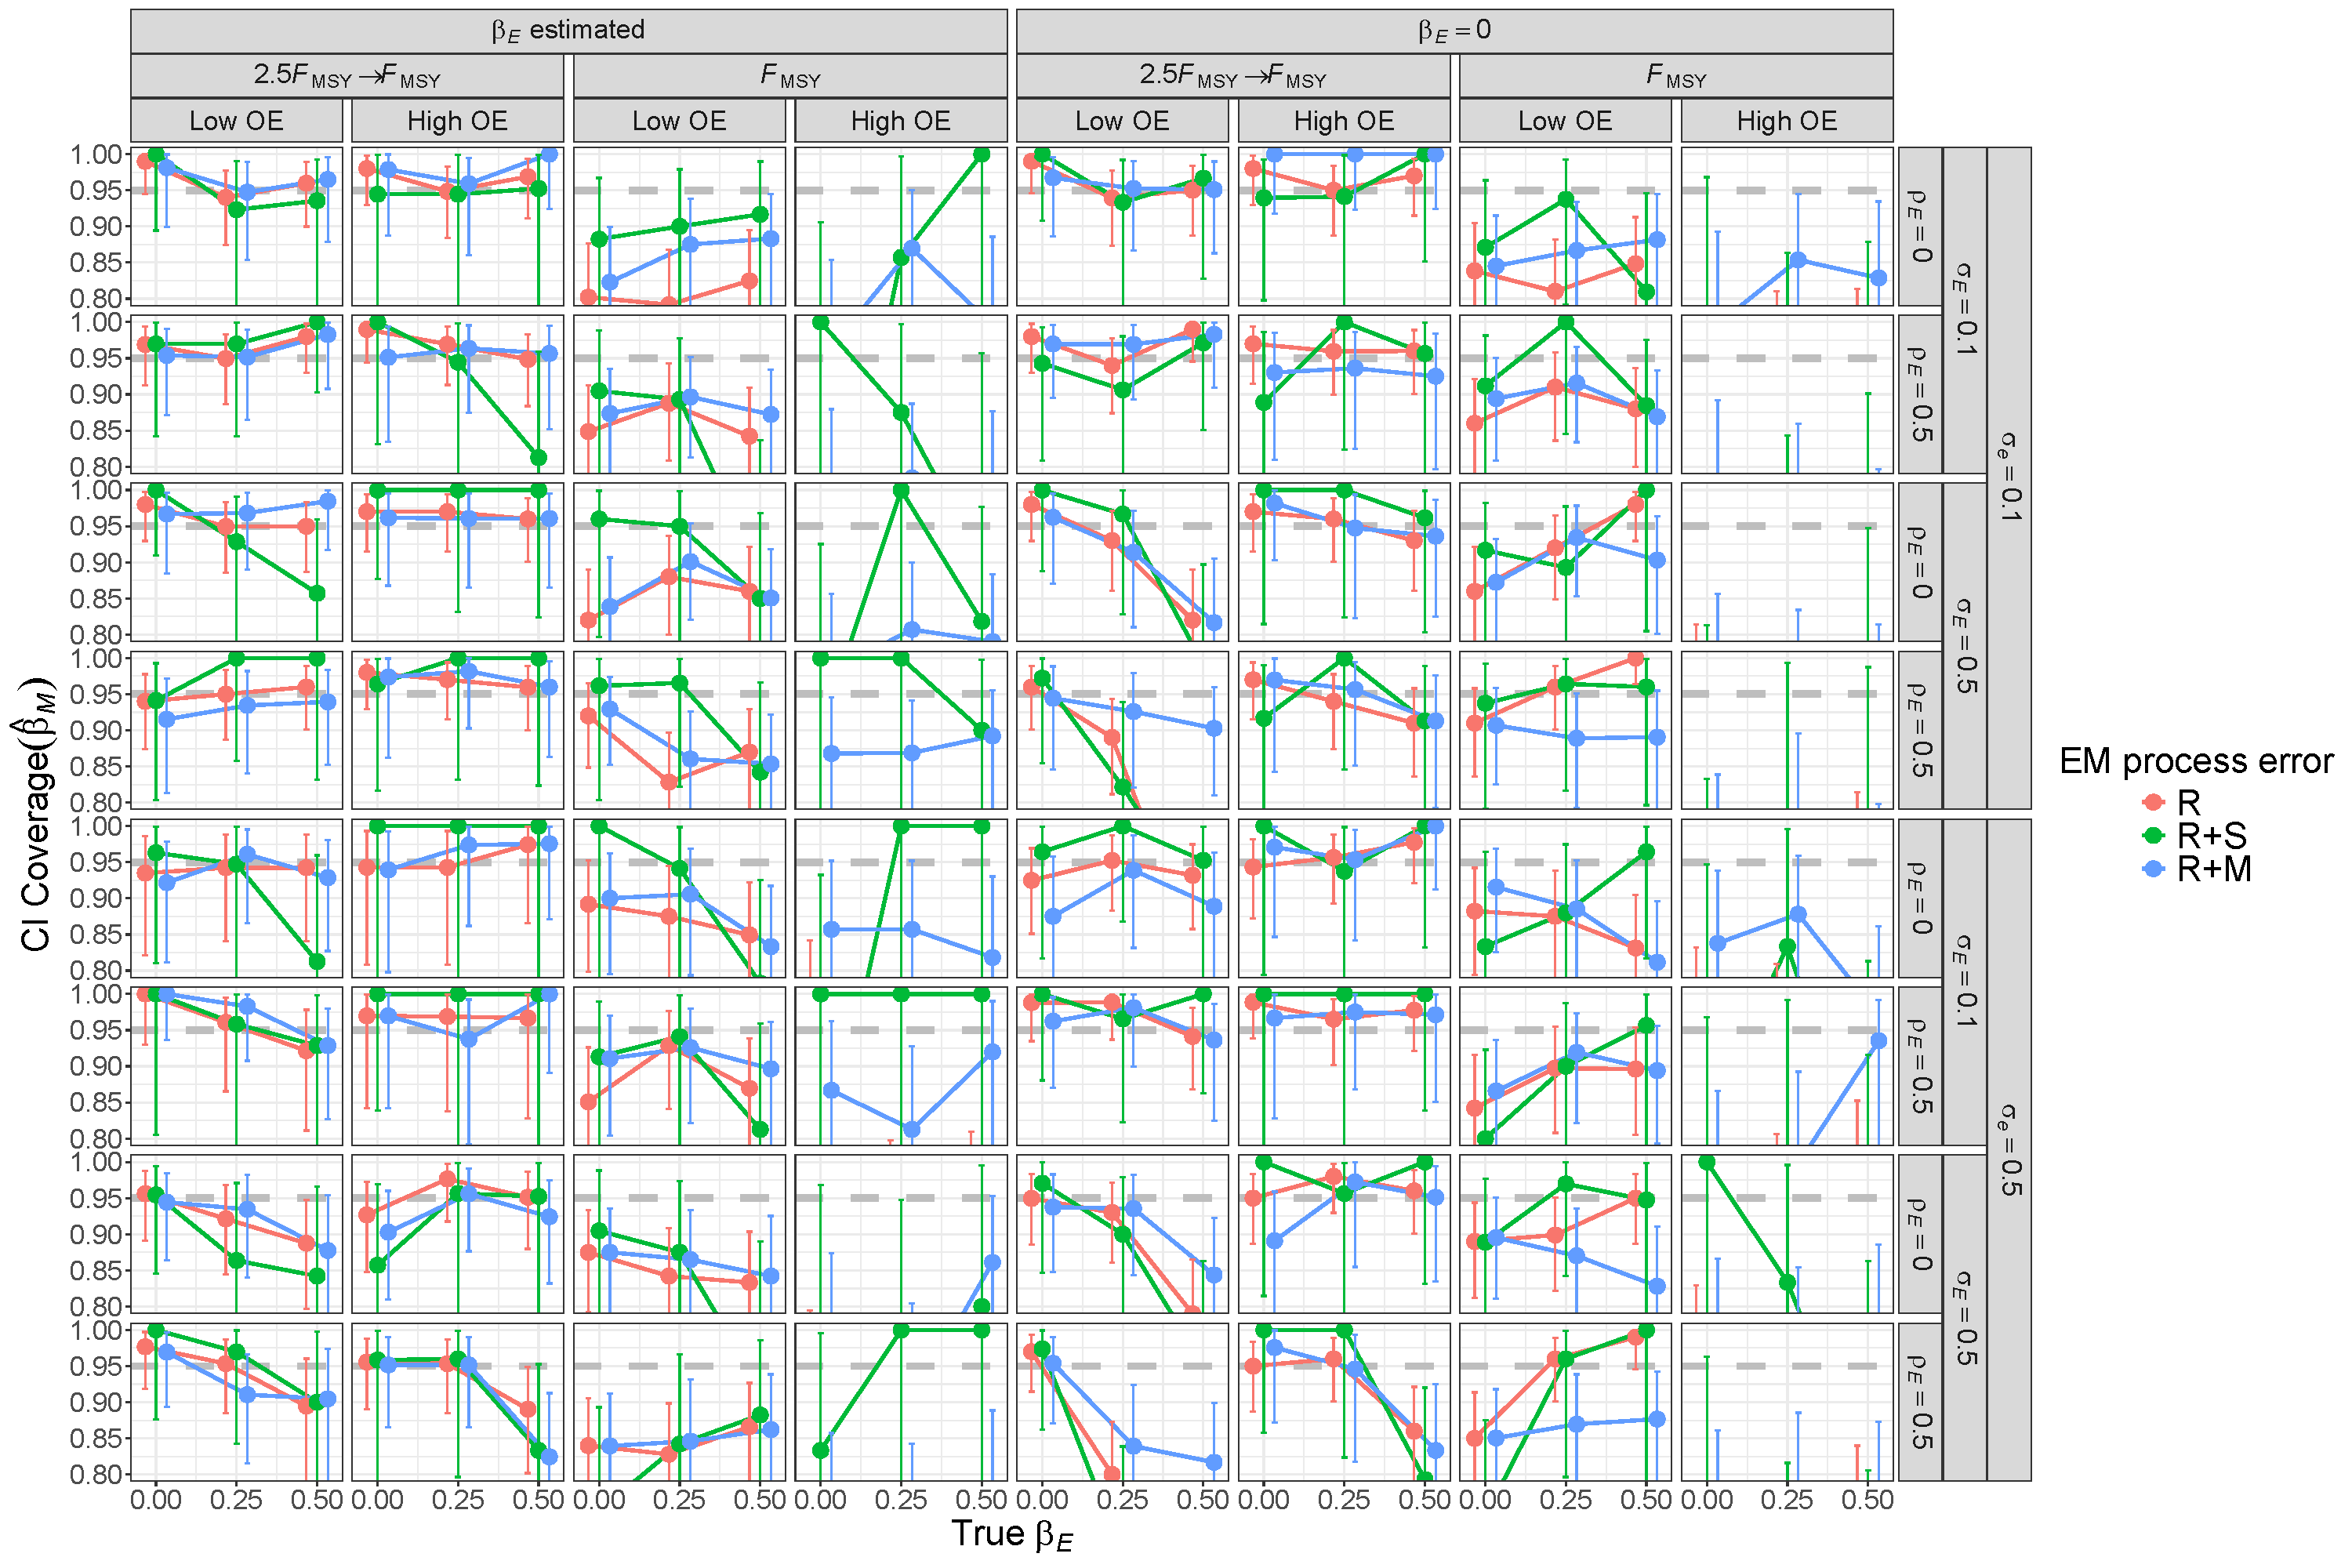
\includegraphics[height = \textheight]{beta_M_CI_coverage_Rom}
\end{center}
\caption{For R OMs, probability of 95\% confidence interval for $\beta_M$ containing the true value for EMs with alternative process error assumptions and treatment of covariate effect ($\beta_E = 0$ or estimated). Vertical lines represent 95\% confidence intervals.}\label{beta_M_CI_coverage_Rom}
\end{figure}
\end{landscape}

\begin{landscape}
\begin{figure}
\begin{center}
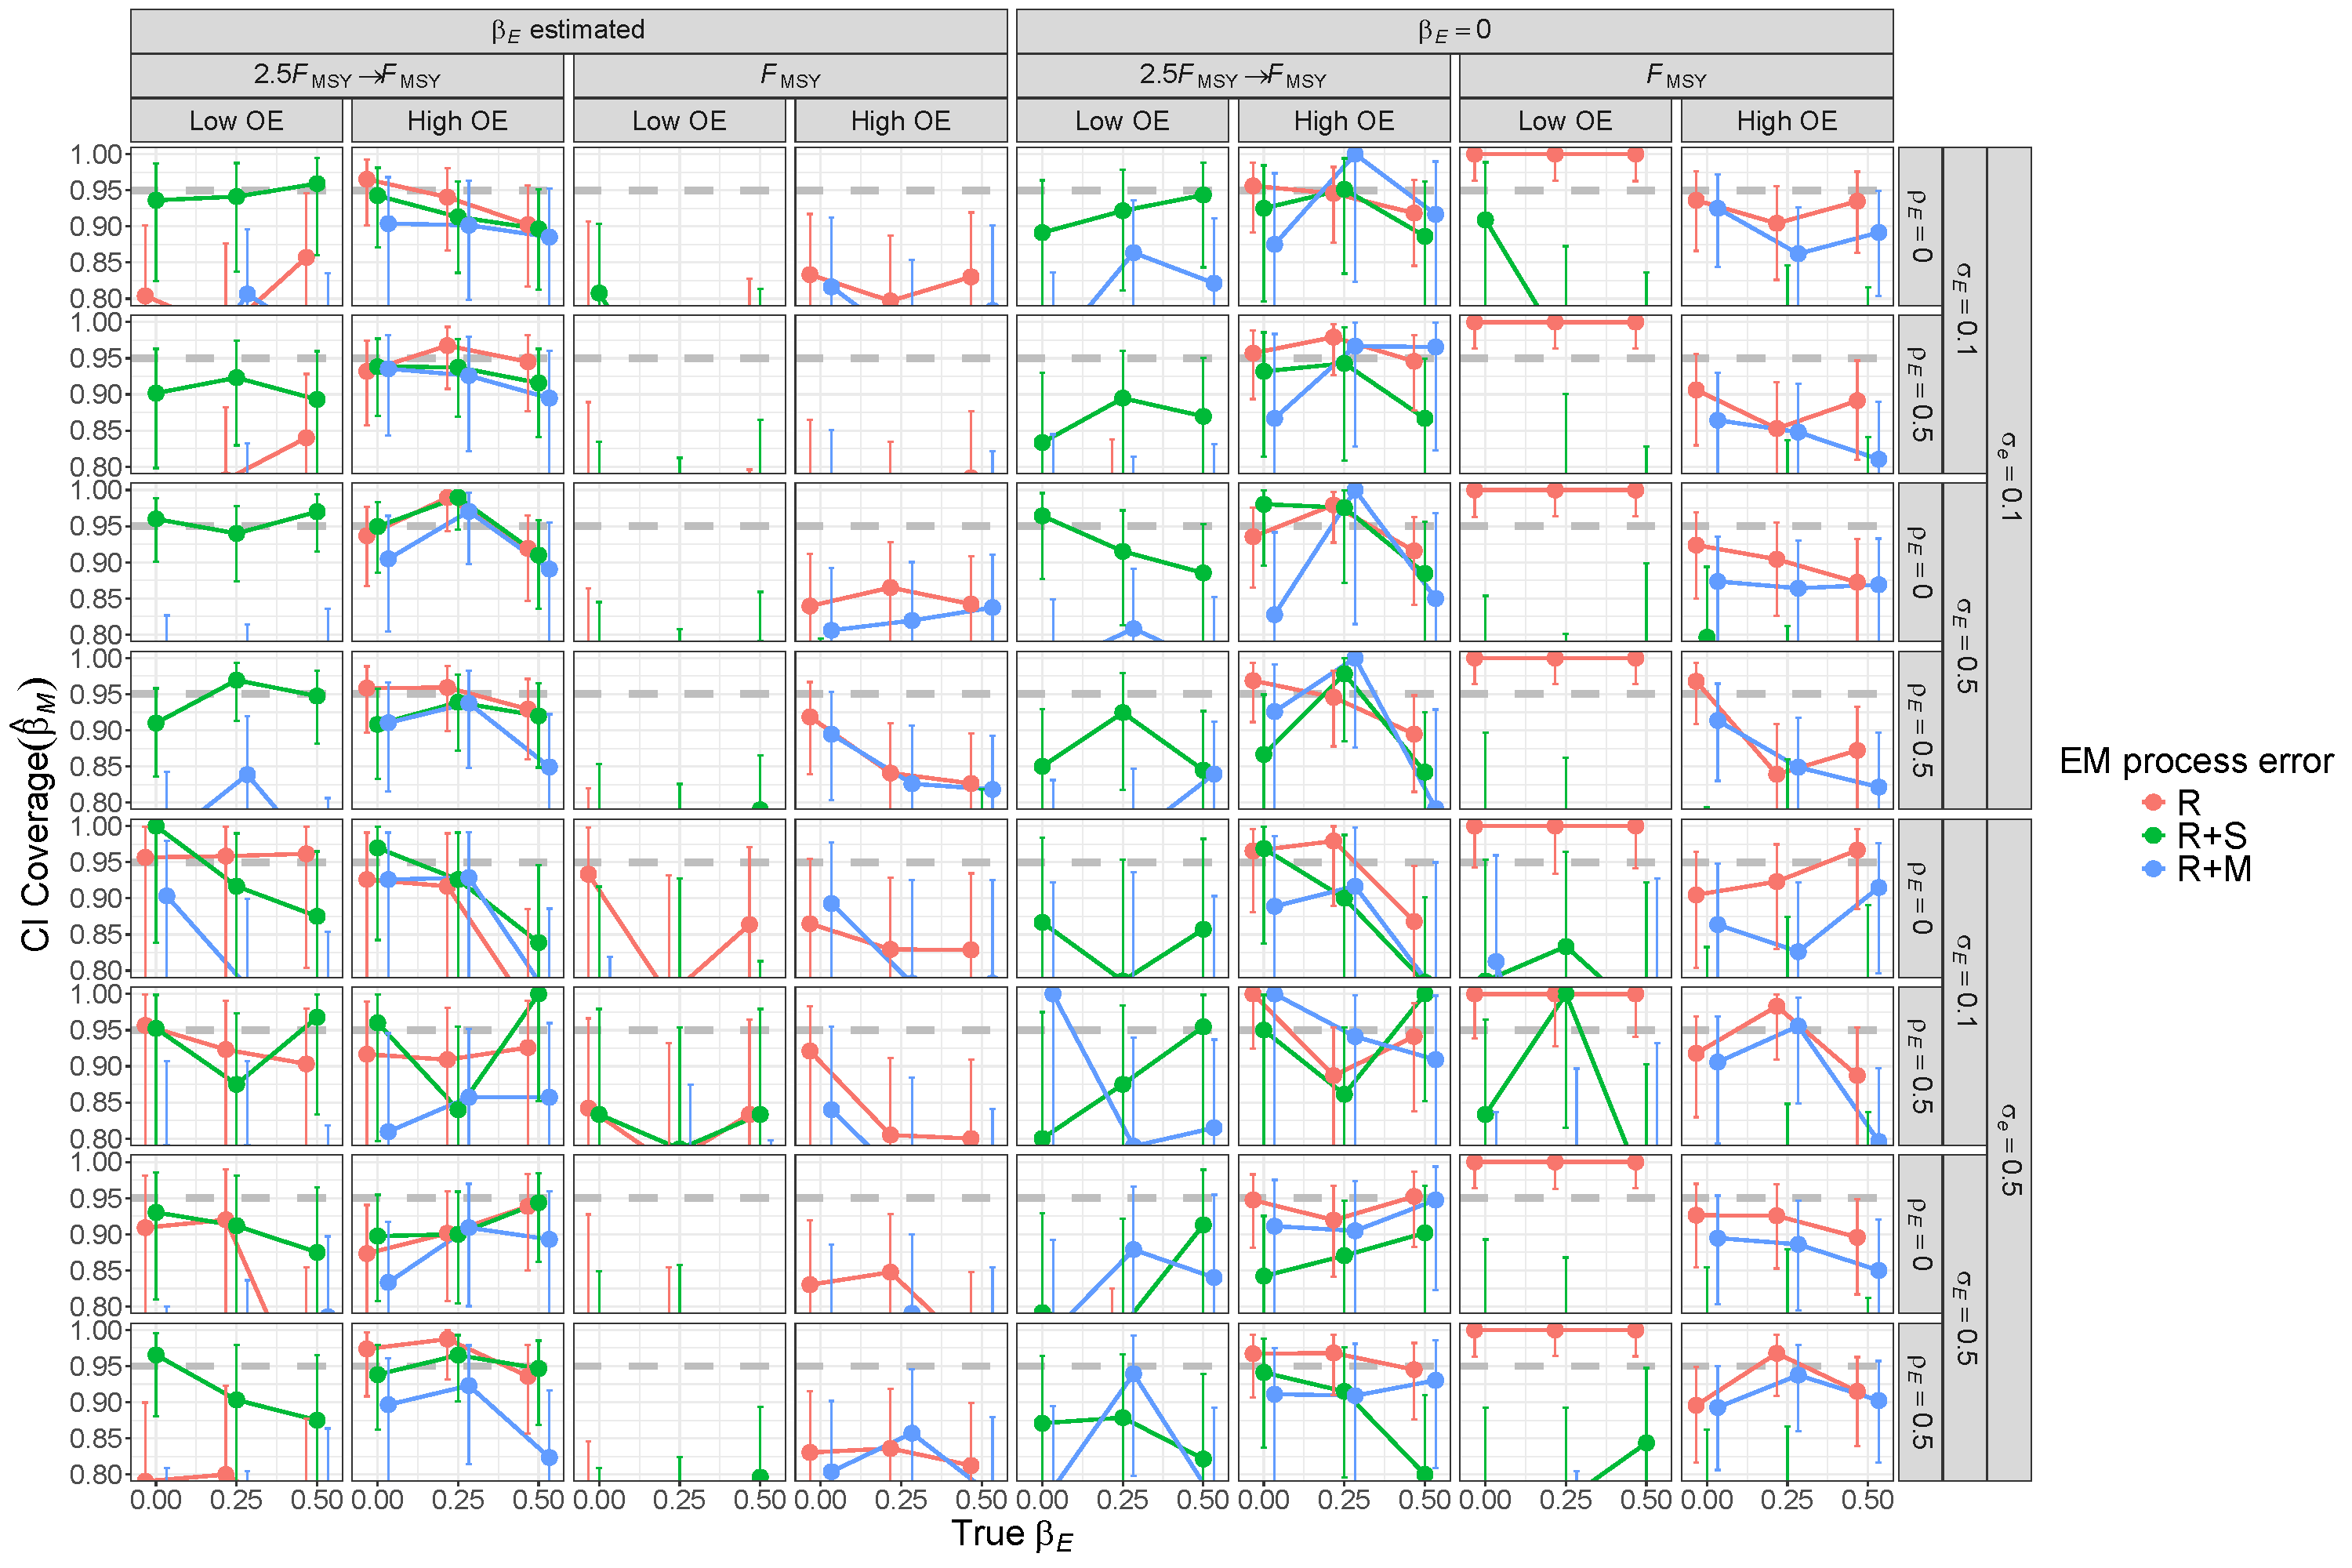
\includegraphics[height = \textheight]{beta_M_CI_coverage_RSom}
\end{center}
\caption{For R+S OMs, probability of 95\% confidence interval for $\beta_M$ containing the true value for EMs with alternative process error assumptions and treatment of covariate effect ($\beta_E = 0$ or estimated). Vertical lines represent 95\% confidence intervals.}\label{beta_M_CI_coverage_RSom}
\end{figure}
\end{landscape}

\begin{landscape}
\begin{figure}
\begin{center}
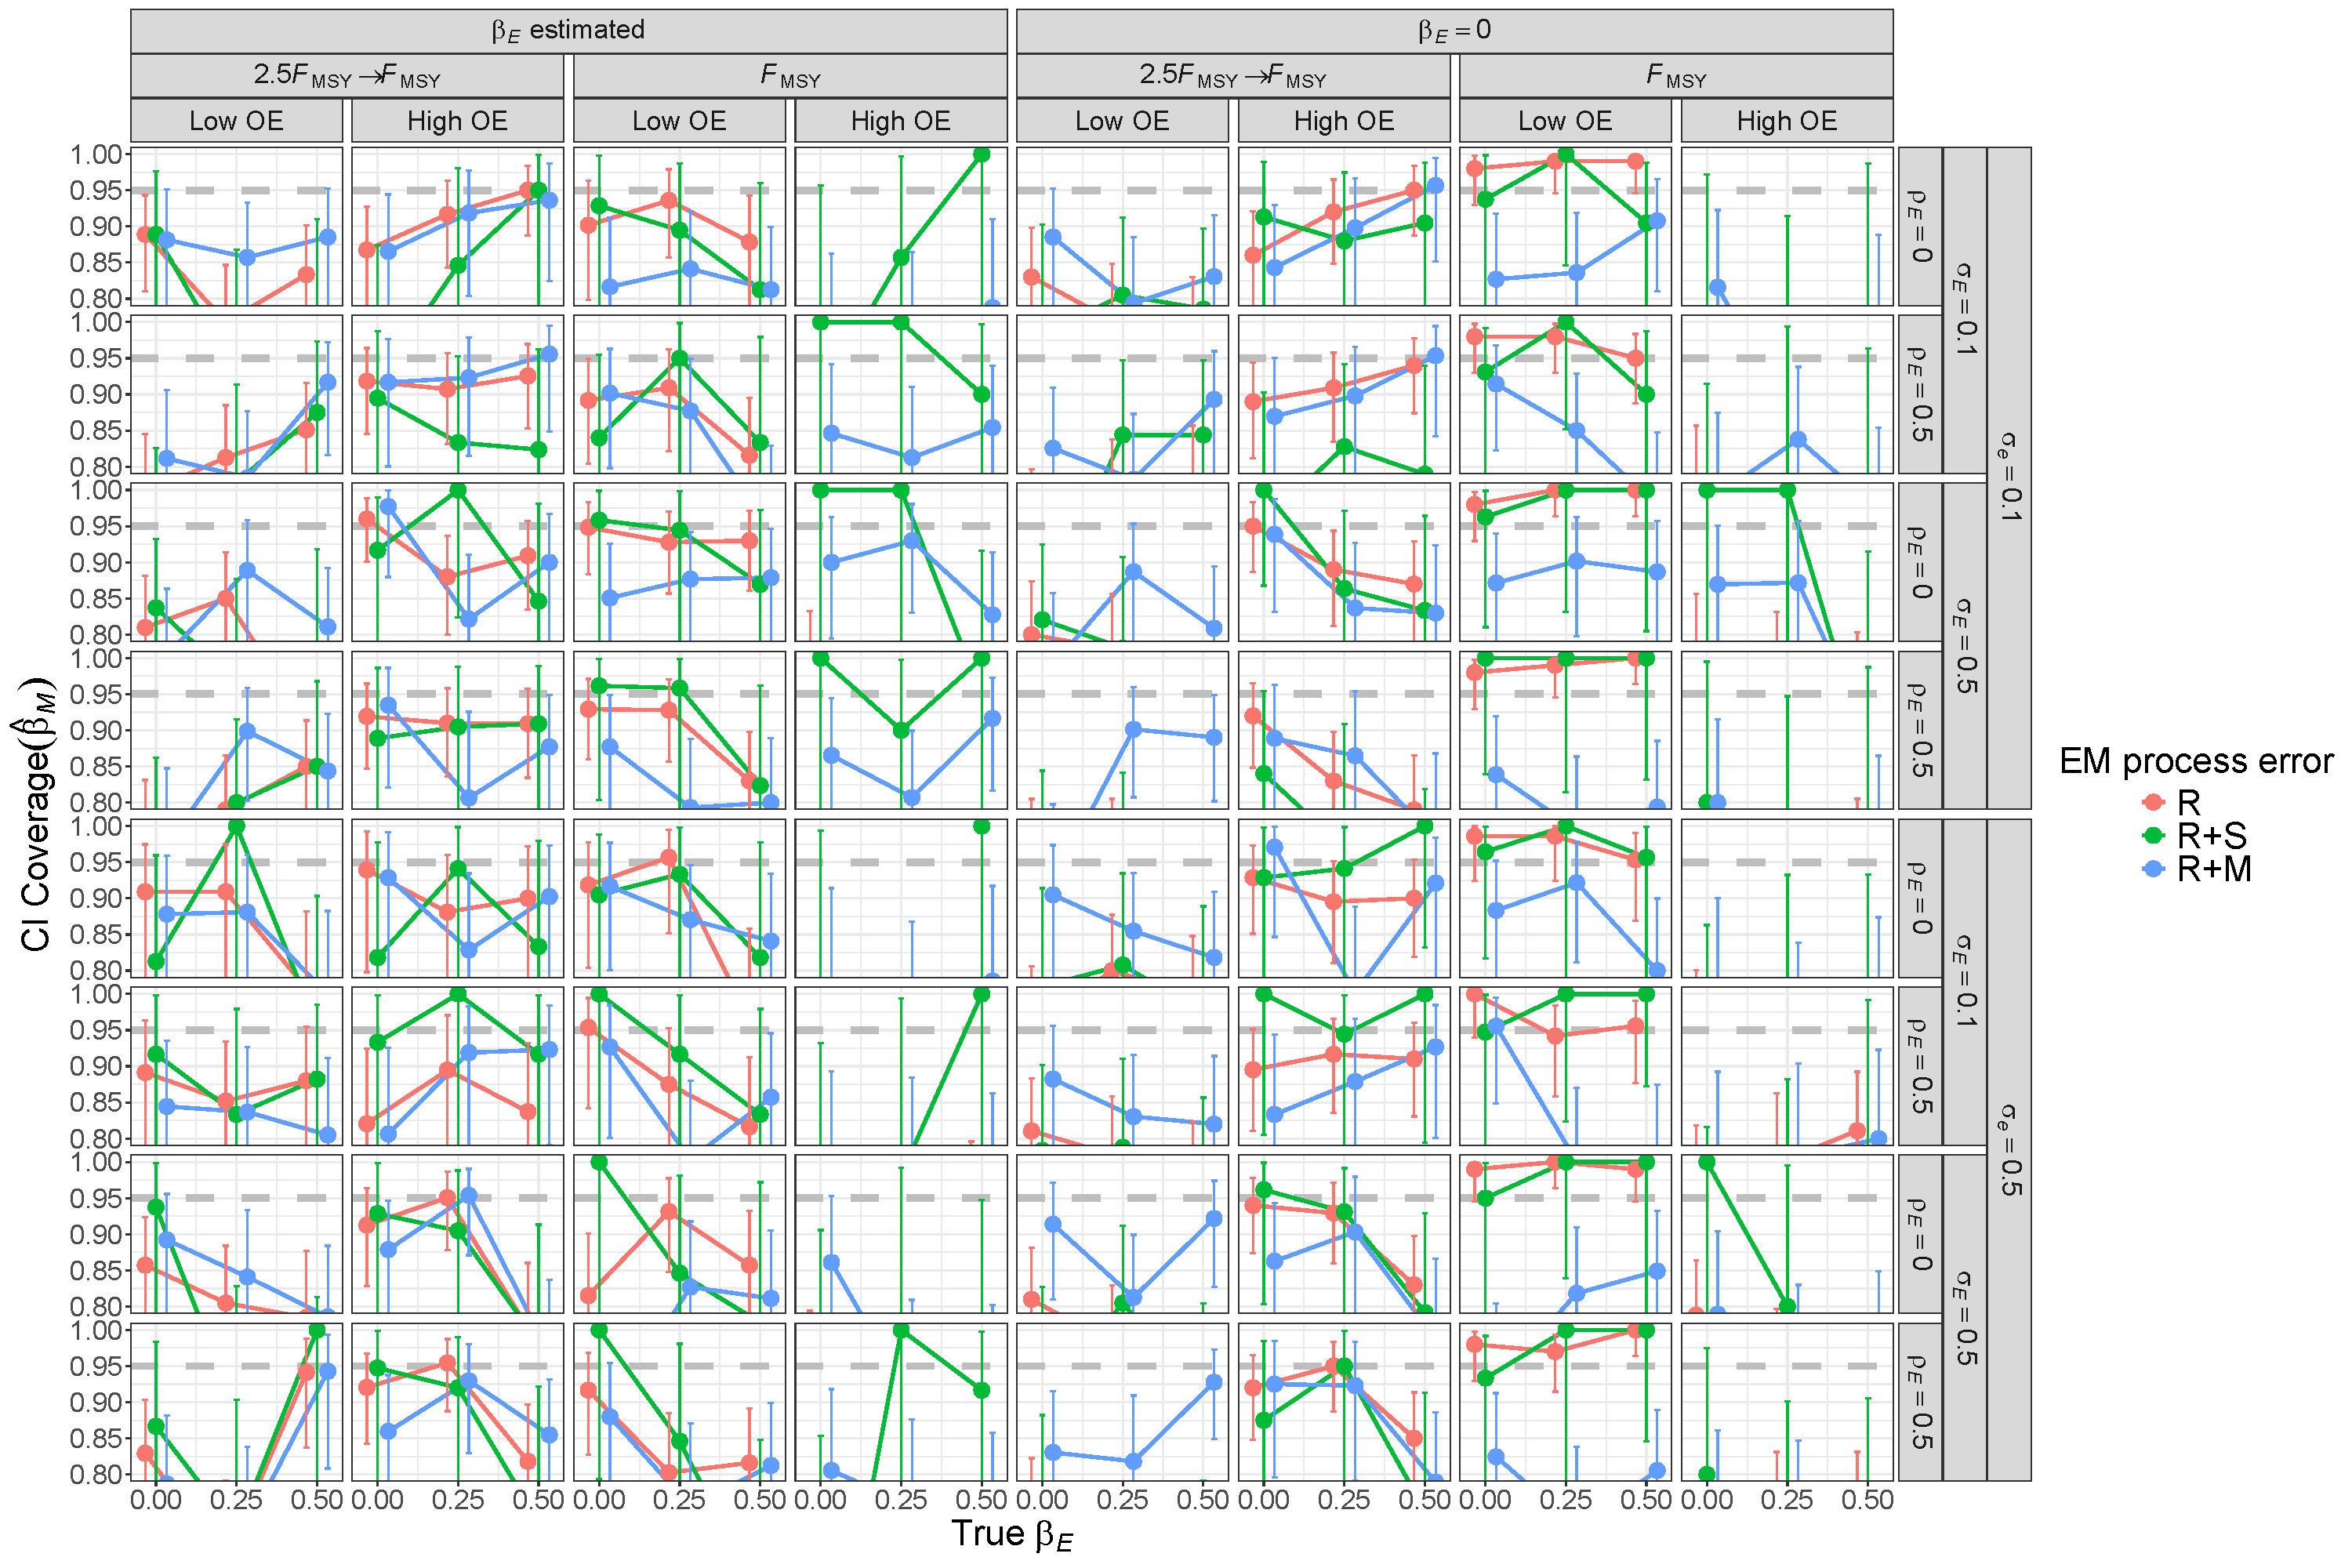
\includegraphics[height = \textheight]{beta_M_CI_coverage_RMom}
\end{center}
\caption{For R+M OMs, probability of 95\% confidence interval for $\beta_M$ containing the true value for EMs with alternative process error assumptions and treatment of covariate effect ($\beta_E = 0$ or estimated). Vertical lines represent 95\% confidence intervals.}\label{beta_M_CI_coverage_RMom}
\end{figure}
\end{landscape}

\DIFdelbegin %DIFDELCMD < \hypertarget{median-natural-mortality-parameter-estimate-and-standard-error-example}{%
%DIFDELCMD < \subsection*{Median natural mortality parameter estimate and standard error example}\label{median-natural-mortality-parameter-estimate-and-standard-error-example}}
%DIFDELCMD < %%%
\DIFdelend \DIFaddbegin \subsection*{\DIFadd{Median natural mortality parameter estimate and standard error example}}\label{median-natural-mortality-parameter-estimate-and-standard-error-example}
\DIFaddend \addcontentsline{toc}{subsection}{Median natural mortality parameter estimate and standard error example}

\begin{landscape}
\begin{figure}
\begin{center}
\DIFdelbeginFL %DIFDELCMD < 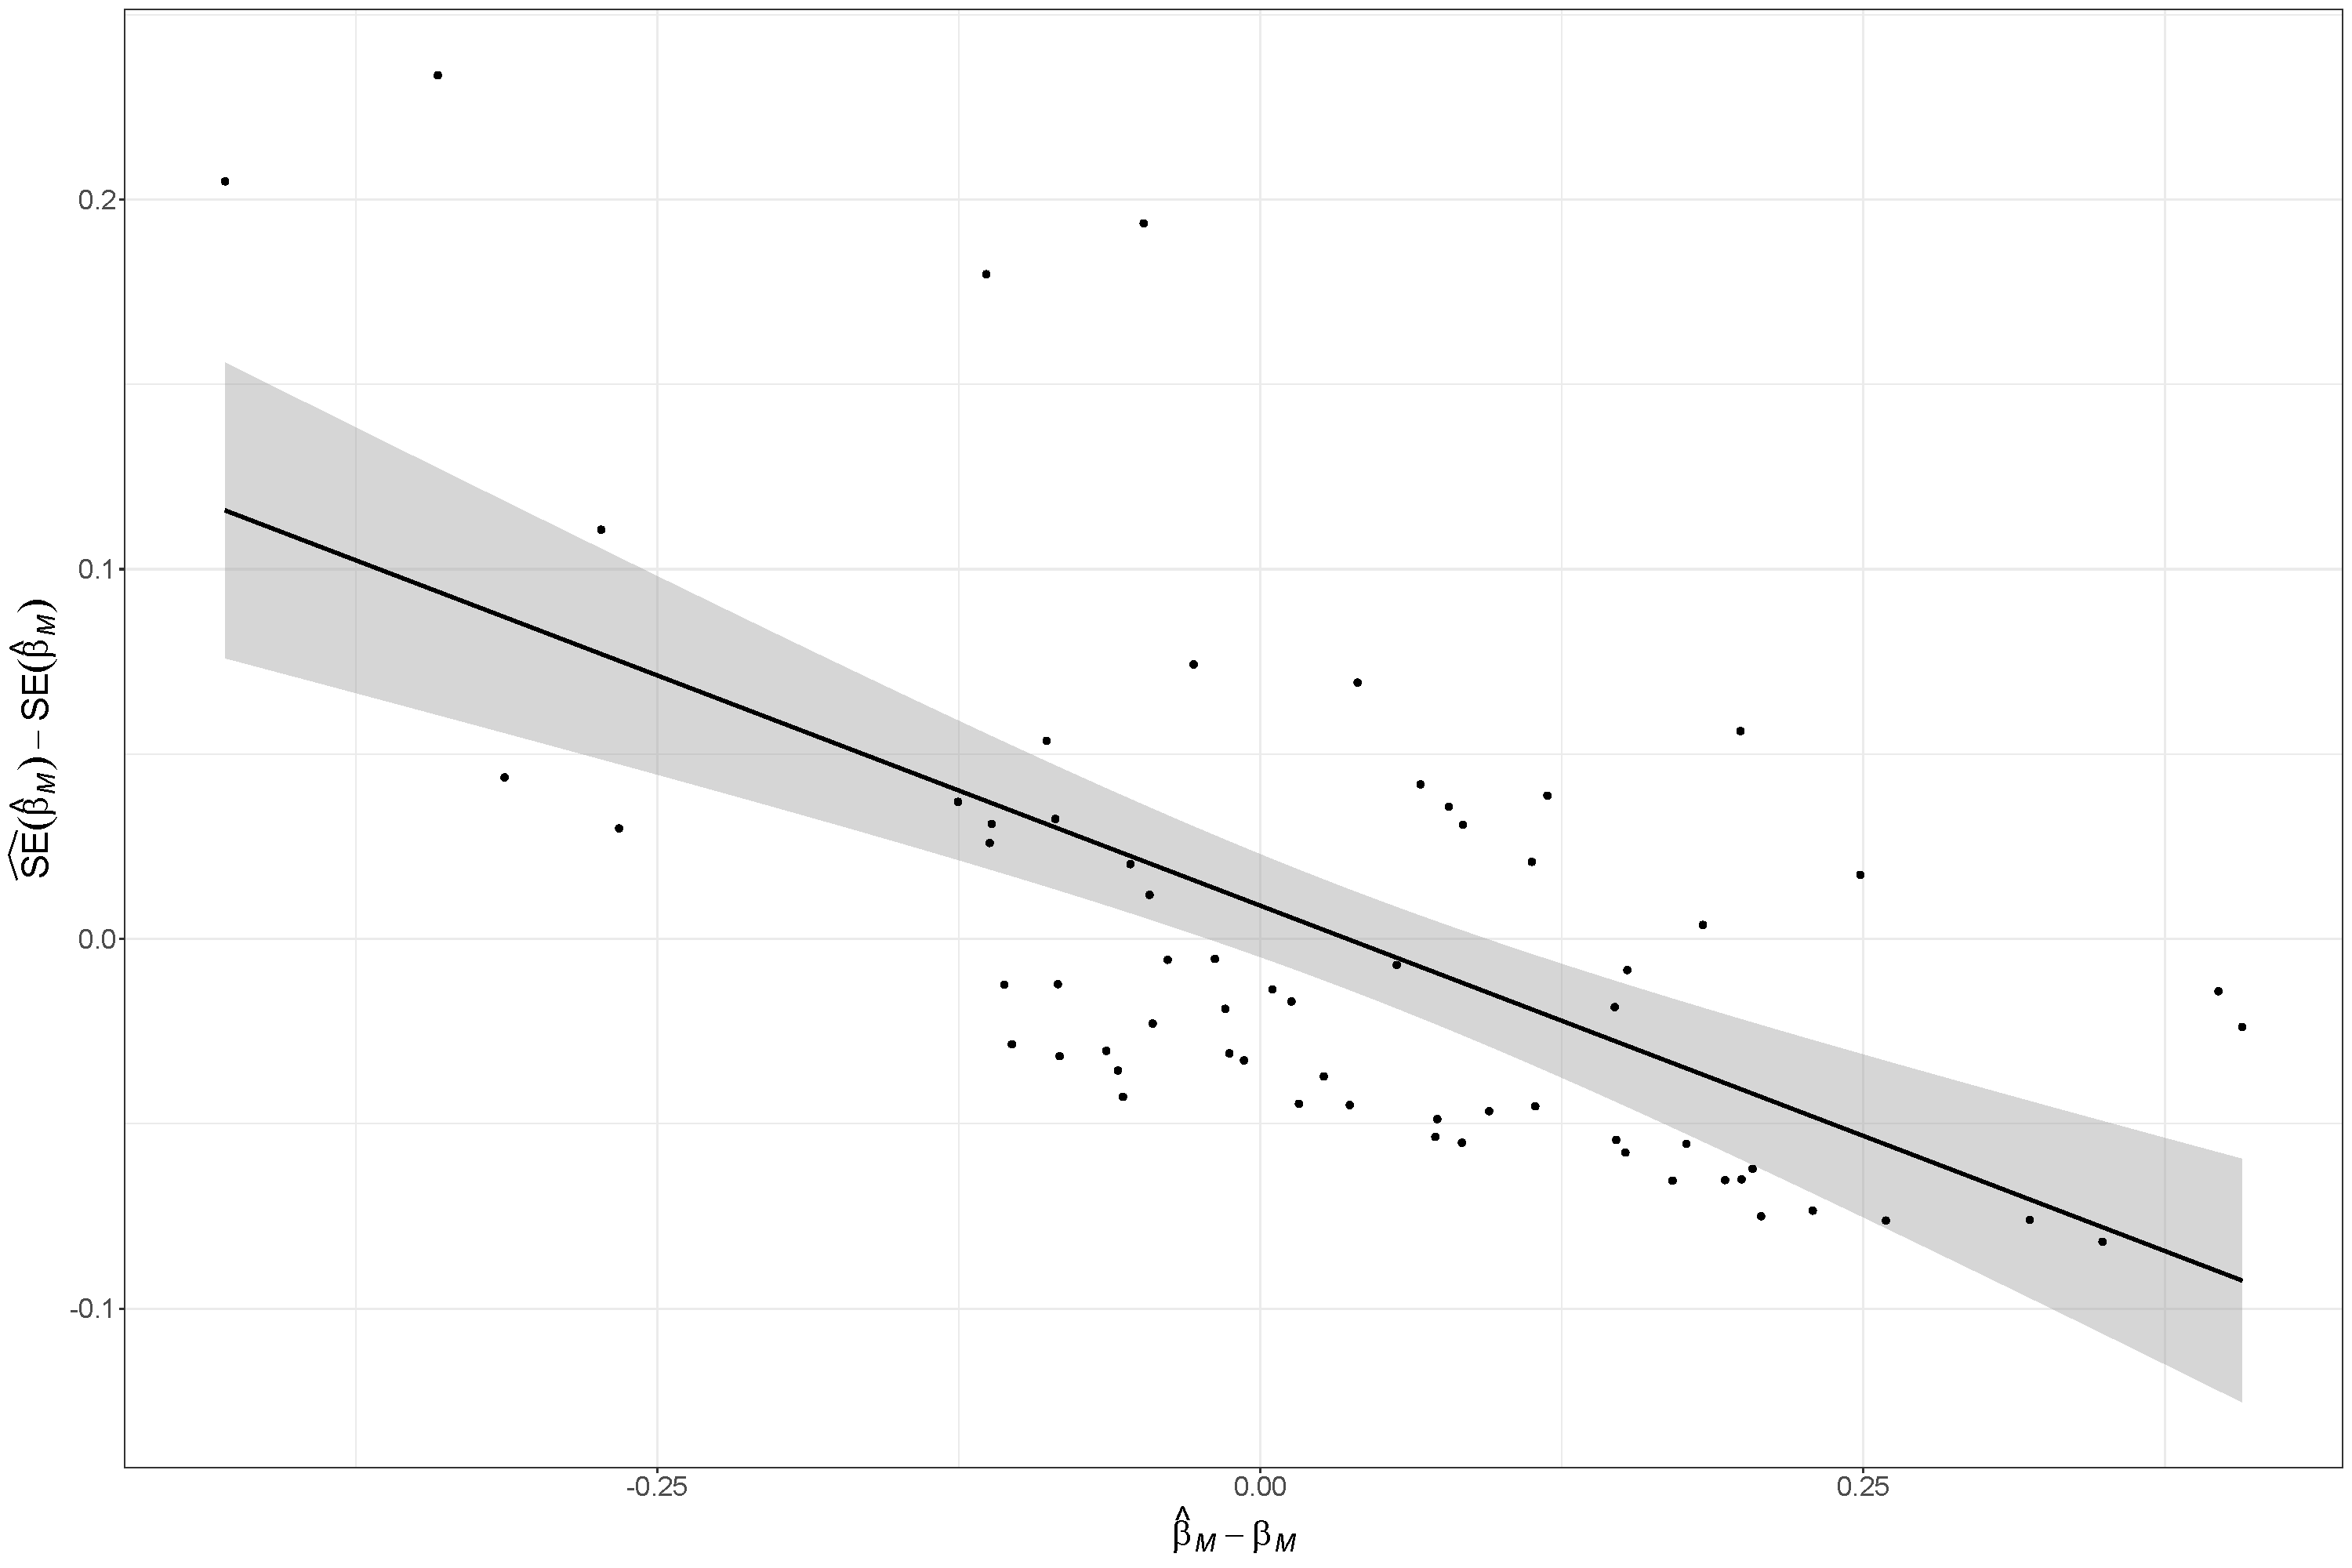
\includegraphics[height = \textheight]{om_69_em_5_beta_M_se_beta_M_lm_plot}
%DIFDELCMD < %%%
\DIFdelendFL \DIFaddbeginFL 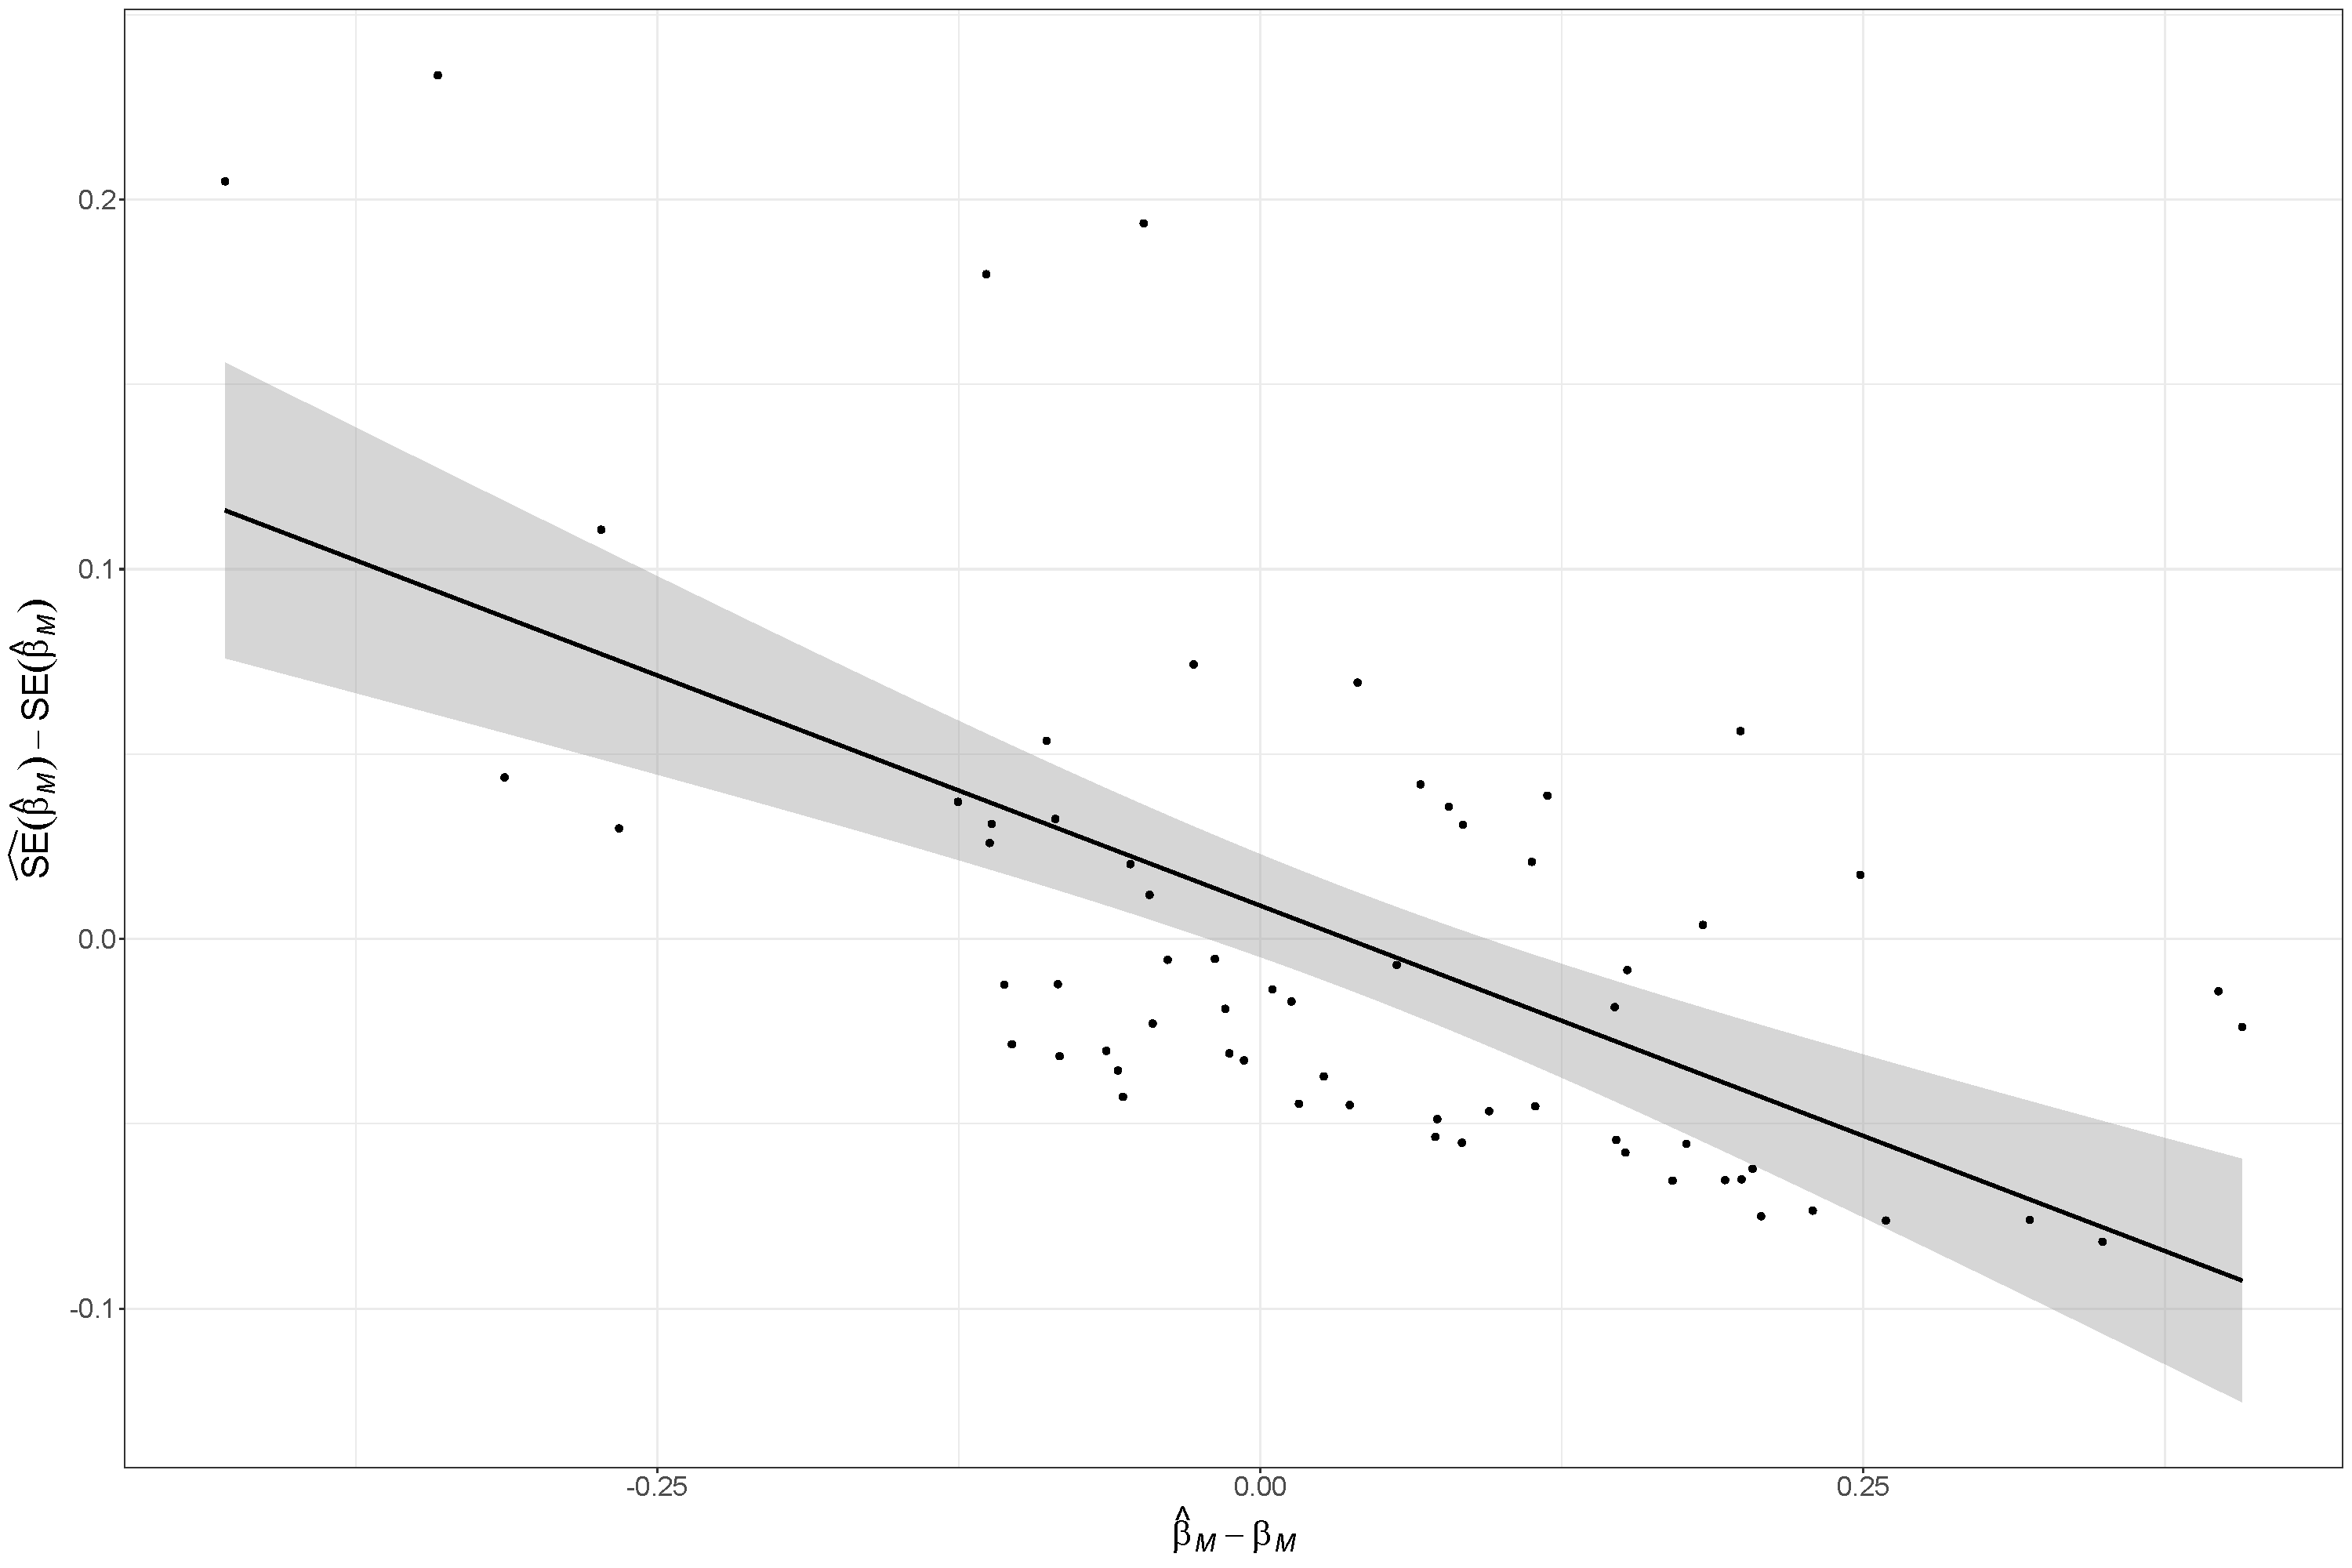
\includegraphics[height = 0.9\textheight]{om_69_em_5_beta_M_se_beta_M_lm_plot}
\DIFaddendFL \end{center}
\caption{Negative correlation of $\beta_M$ estimates and Hessian-based standard error estimates for EM that also estimates the covariate effect and has correct R+M process error assumption fitted to simulated data from the OM with R+M process errors, temporal contrast in fishing pressure, low observation uncertainty for both population ($Low OE$) and covariate observations ($\sigma_e = 0.1$), high and uncorrelated temporal variability in the true covariate ($\sigma_E = 0.5$ and $\rho_E = 0$), and the strongest covariate effect on \DIFdelbeginFL \DIFdelFL{natural mortality }\DIFdelendFL \DIFaddbeginFL \DIFaddFL{$M$ }\DIFaddendFL ($\beta_E = 0.5$).}\label{ex_lm_beta_M_SE_beta_M}
\end{figure}
\end{landscape}

\DIFdelbegin %DIFDELCMD < \hypertarget{median-natural-mortality-parameter-rmse}{%
%DIFDELCMD < \subsection*{Median Natural mortality parameter RMSE}\label{median-natural-mortality-parameter-rmse}}
%DIFDELCMD < %%%
\DIFdelend \DIFaddbegin \subsection*{\DIFadd{Median Natural mortality parameter accuracy}}\label{median-natural-mortality-parameter-accuracy}
\DIFaddend \addcontentsline{toc}{subsection}{Median Natural mortality parameter \DIFdelbegin \DIFdel{RMSE}\DIFdelend \DIFaddbegin \DIFadd{accuracy}\DIFaddend }

\begin{landscape}
\begin{figure}
\begin{center}
\DIFdelbeginFL %DIFDELCMD < 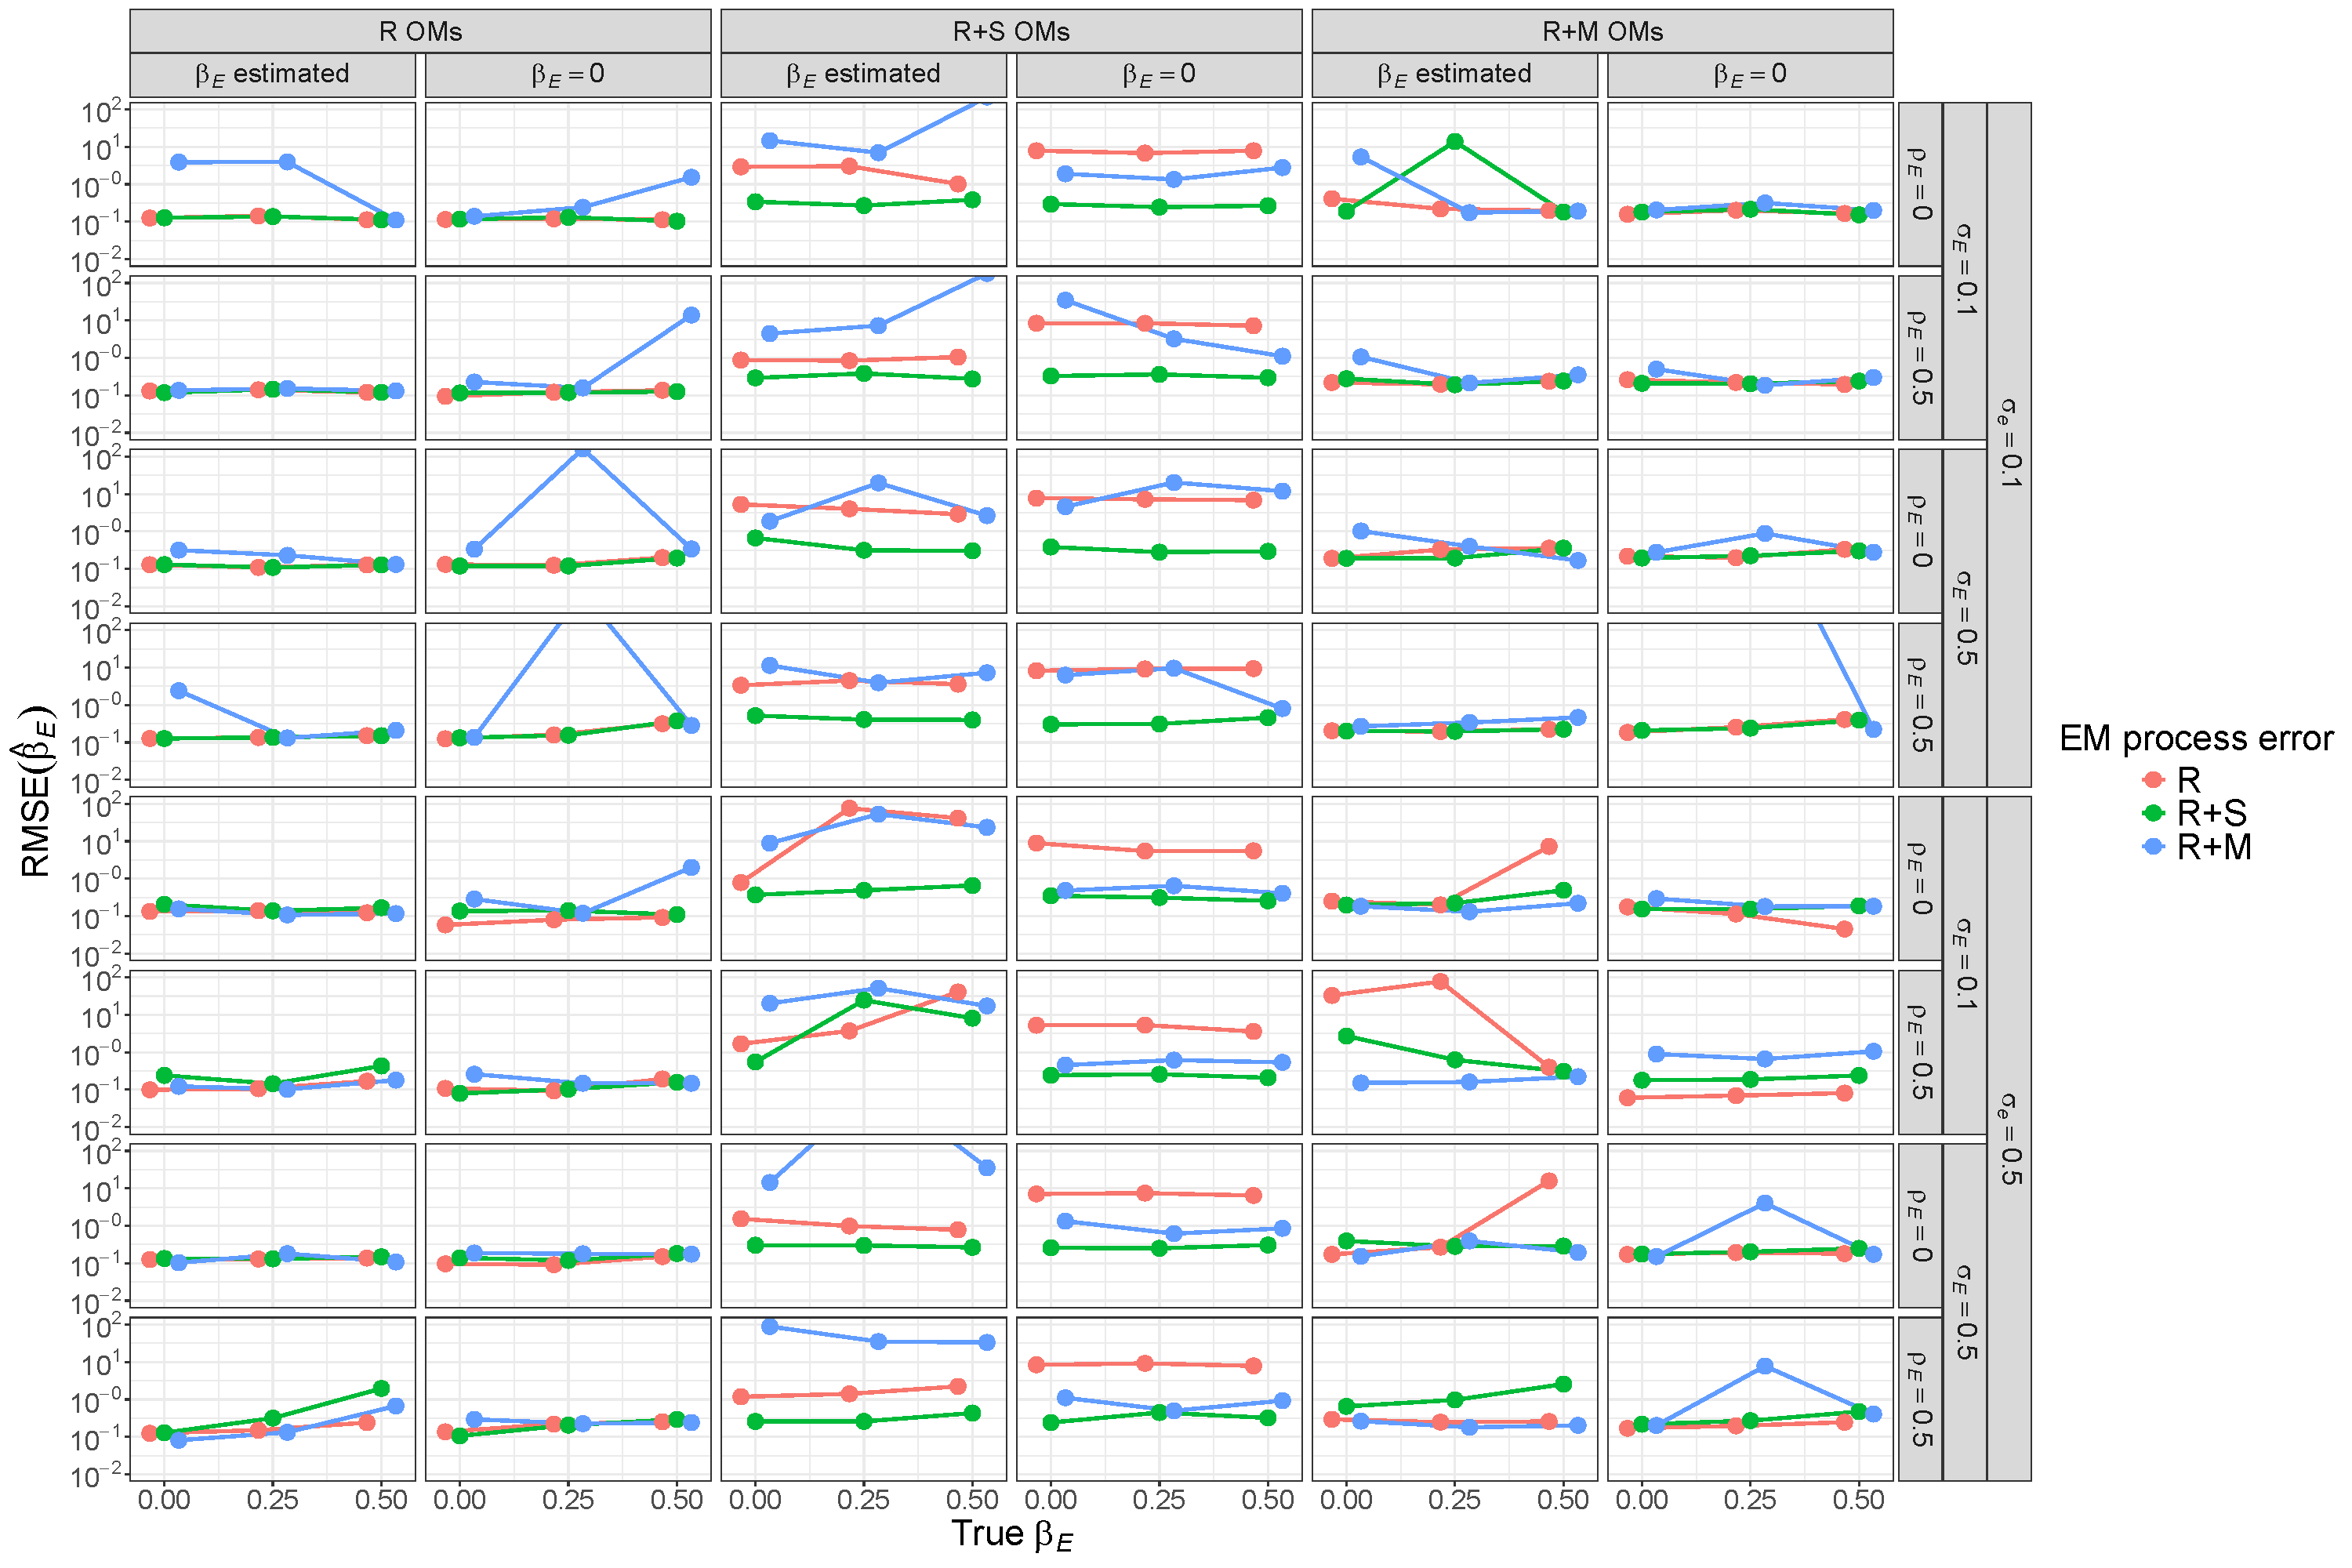
\includegraphics[height = \textheight]{beta_M_rmse_main}
%DIFDELCMD < %%%
\DIFdelendFL \DIFaddbeginFL 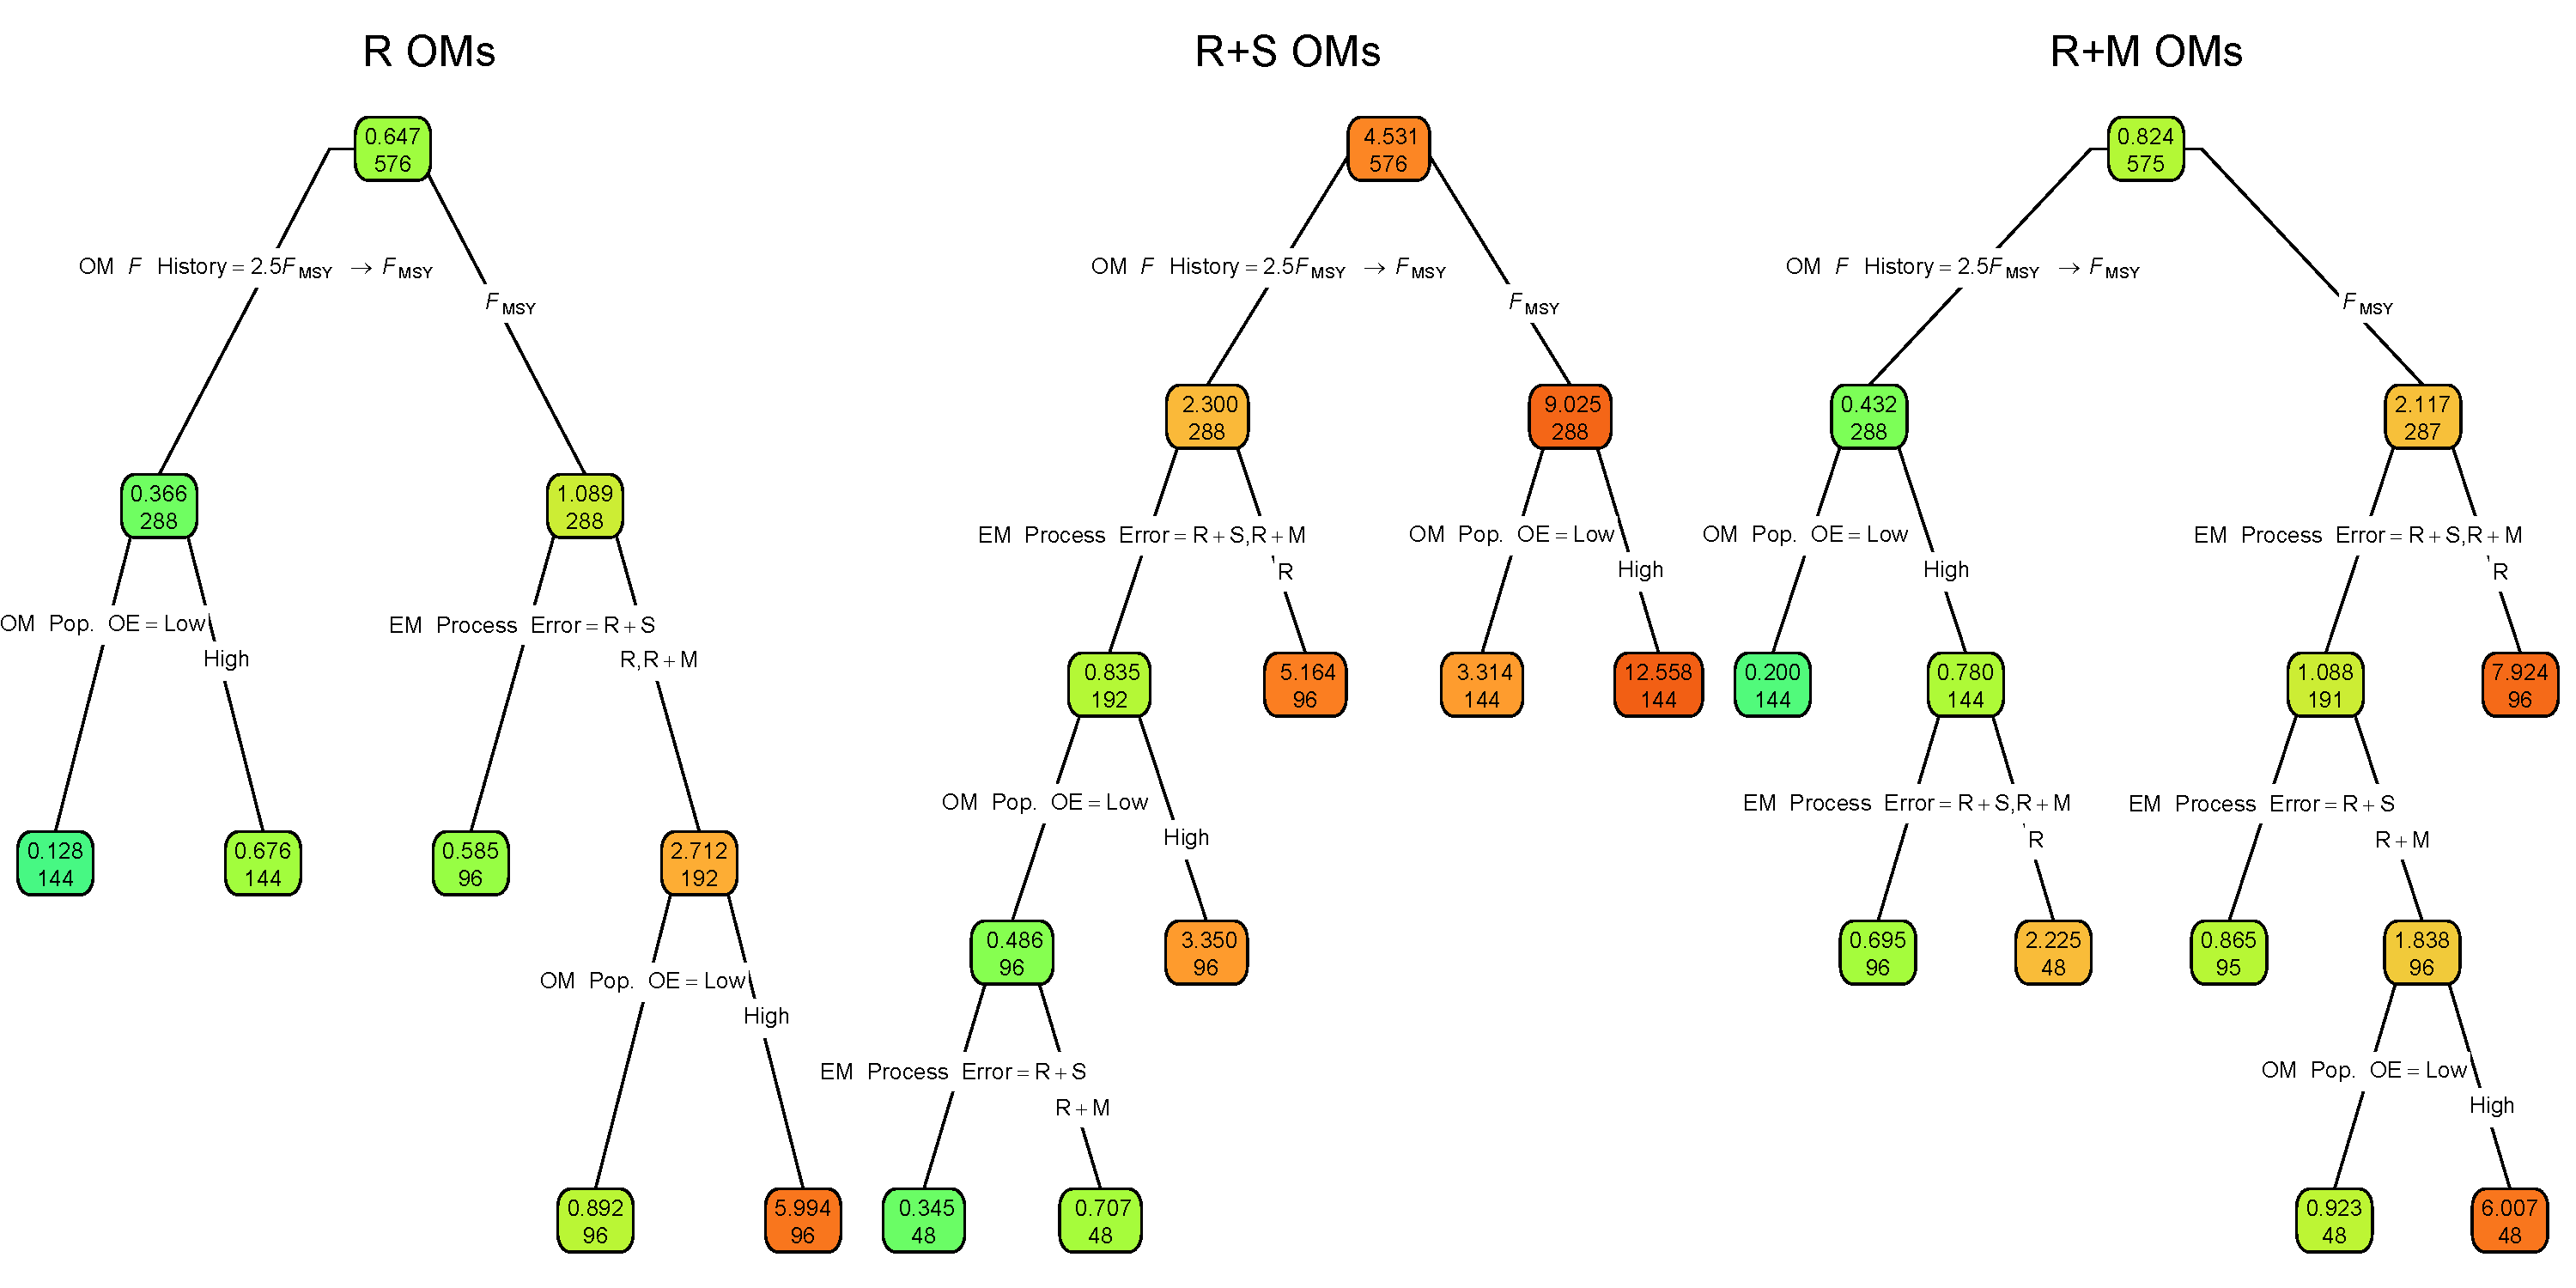
\includegraphics[width = 1.4\textwidth]{median_M_rmse_regtree_plots}
\DIFaddendFL \end{center}
\caption{\DIFdelbeginFL \DIFdelFL{Root mean square error  (}\DIFdelendFL \DIFaddbeginFL \DIFaddFL{Regression trees indicating primary factors determining reductions in sums of squares of errors for the log-transformed }\DIFaddendFL RMSE \DIFdelbeginFL \DIFdelFL{) }\DIFdelendFL of estimates \DIFdelbeginFL \DIFdelFL{of  $\beta_M$ from fitting }\DIFdelendFL \DIFaddbeginFL \DIFaddFL{for the median $M$ parameter ($\text{RMSE}\left(\widehat \beta_M\right)$) in }\DIFaddendFL EMs \DIFaddbeginFL \DIFaddFL{fitted to operating models (OMs) }\DIFaddendFL with \DIFdelbeginFL \DIFdelFL{alternative }\DIFdelendFL process error \DIFdelbeginFL \DIFdelFL{assumptions }\DIFdelendFL \DIFaddbeginFL \DIFaddFL{on recruitment only (R), recruitment }\DIFaddendFL and \DIFdelbeginFL \DIFdelFL{treatment of covariate effect }\DIFdelendFL \DIFaddbeginFL \DIFaddFL{apparent survival }\DIFaddendFL (\DIFdelbeginFL \DIFdelFL{$\beta_E = 0$ }\DIFdelendFL \DIFaddbeginFL \DIFaddFL{R+S), }\DIFaddendFL or \DIFdelbeginFL \DIFdelFL{estimated}\DIFdelendFL \DIFaddbeginFL \DIFaddFL{recruitment and natural mortality (R+M}\DIFaddendFL ). \DIFdelbeginFL \DIFdelFL{All OMs had low observation }\DIFdelendFL \DIFaddbeginFL \DIFaddFL{Each node shows the median }\DIFaddendFL error \DIFdelbeginFL \DIFdelFL{for population observations }\DIFdelendFL \DIFaddbeginFL \DIFaddFL{(top) }\DIFaddendFL and \DIFdelbeginFL \DIFdelFL{contrast in fishing mortality}\DIFdelendFL \DIFaddbeginFL \DIFaddFL{number of observations (bottom) for the corresponding subset}\DIFaddendFL . \DIFaddbeginFL \DIFaddFL{Lower or higher median RMSE are indicated by more green or red polygons, respectively.}\DIFaddendFL }\DIFdelbeginFL %DIFDELCMD < \label{beta_M_rmse}
%DIFDELCMD < %%%
\DIFdelendFL \DIFaddbeginFL \label{med_M_rmse_regtree}
\DIFaddendFL \end{figure}
\end{landscape}

\DIFaddbegin \begin{table}
\caption{\DIFaddFL{For each OM process error source (columns), percent reduction in deviance for linear regression models fit to the log-transformed RMSE for estimates of the median $M$ parameter ($\text{RMSE}\left(\widehat \beta_M\right)$) with each OM and EM factor (rows) included individually, combined, and with second and third order interactions.}}\label{RMSE_mean_M_PRD_table}
{\begin{center}
\begin{tabular}{lrrr}
\hline\hline
\multicolumn{1}{l}{\DIFaddFL{Factor}}&\multicolumn{1}{c}{\DIFaddFL{R}}&\multicolumn{1}{c}{\DIFaddFL{R+S}}&\multicolumn{1}{c}{\DIFaddFL{R+M}}\tabularnewline
\hline
\DIFaddFL{OM $F$ history}&\DIFaddFL{34.70}&\DIFaddFL{24.62}&\DIFaddFL{34.91}\tabularnewline
\DIFaddFL{OM Obs. Error}&\DIFaddFL{25.55}&\DIFaddFL{17.82}&\DIFaddFL{12.77}\tabularnewline
\DIFaddFL{$OM \sigma_e$}& \DIFaddFL{0.01}&\DIFaddFL{\textless  0.01}&\DIFaddFL{\textless  0.01}\tabularnewline
\DIFaddFL{$OM \sigma_E$}& \DIFaddFL{0.19}& \DIFaddFL{0.02}& \DIFaddFL{0.07}\tabularnewline
\DIFaddFL{$OM \rho_{E}$}& \DIFaddFL{0.05}& \DIFaddFL{0.26}& \DIFaddFL{0.03}\tabularnewline
\DIFaddFL{OM $\beta_{E}$}& \DIFaddFL{0.58}& \DIFaddFL{0.23}& \DIFaddFL{0.16}\tabularnewline
\DIFaddFL{EM Process Error}&\DIFaddFL{10.75}&\DIFaddFL{18.12}&\DIFaddFL{14.50}\tabularnewline
\DIFaddFL{$EM \beta_{E}$ assumption}& \DIFaddFL{3.96}& \DIFaddFL{6.39}& \DIFaddFL{2.93}\tabularnewline
\DIFaddFL{All factors}&\DIFaddFL{75.79}&\DIFaddFL{67.47}&\DIFaddFL{65.26}\tabularnewline
\DIFaddFL{+ All Two Way}&\DIFaddFL{90.21}&\DIFaddFL{80.65}&\DIFaddFL{77.59}\tabularnewline
\DIFaddFL{+ All Three Way}&\DIFaddFL{93.72}&\DIFaddFL{88.68}&\DIFaddFL{86.44}\tabularnewline
\hline
\end{tabular}\end{center}
}
\end{table}

\DIFaddend \begin{landscape}
\begin{figure}
\begin{center}
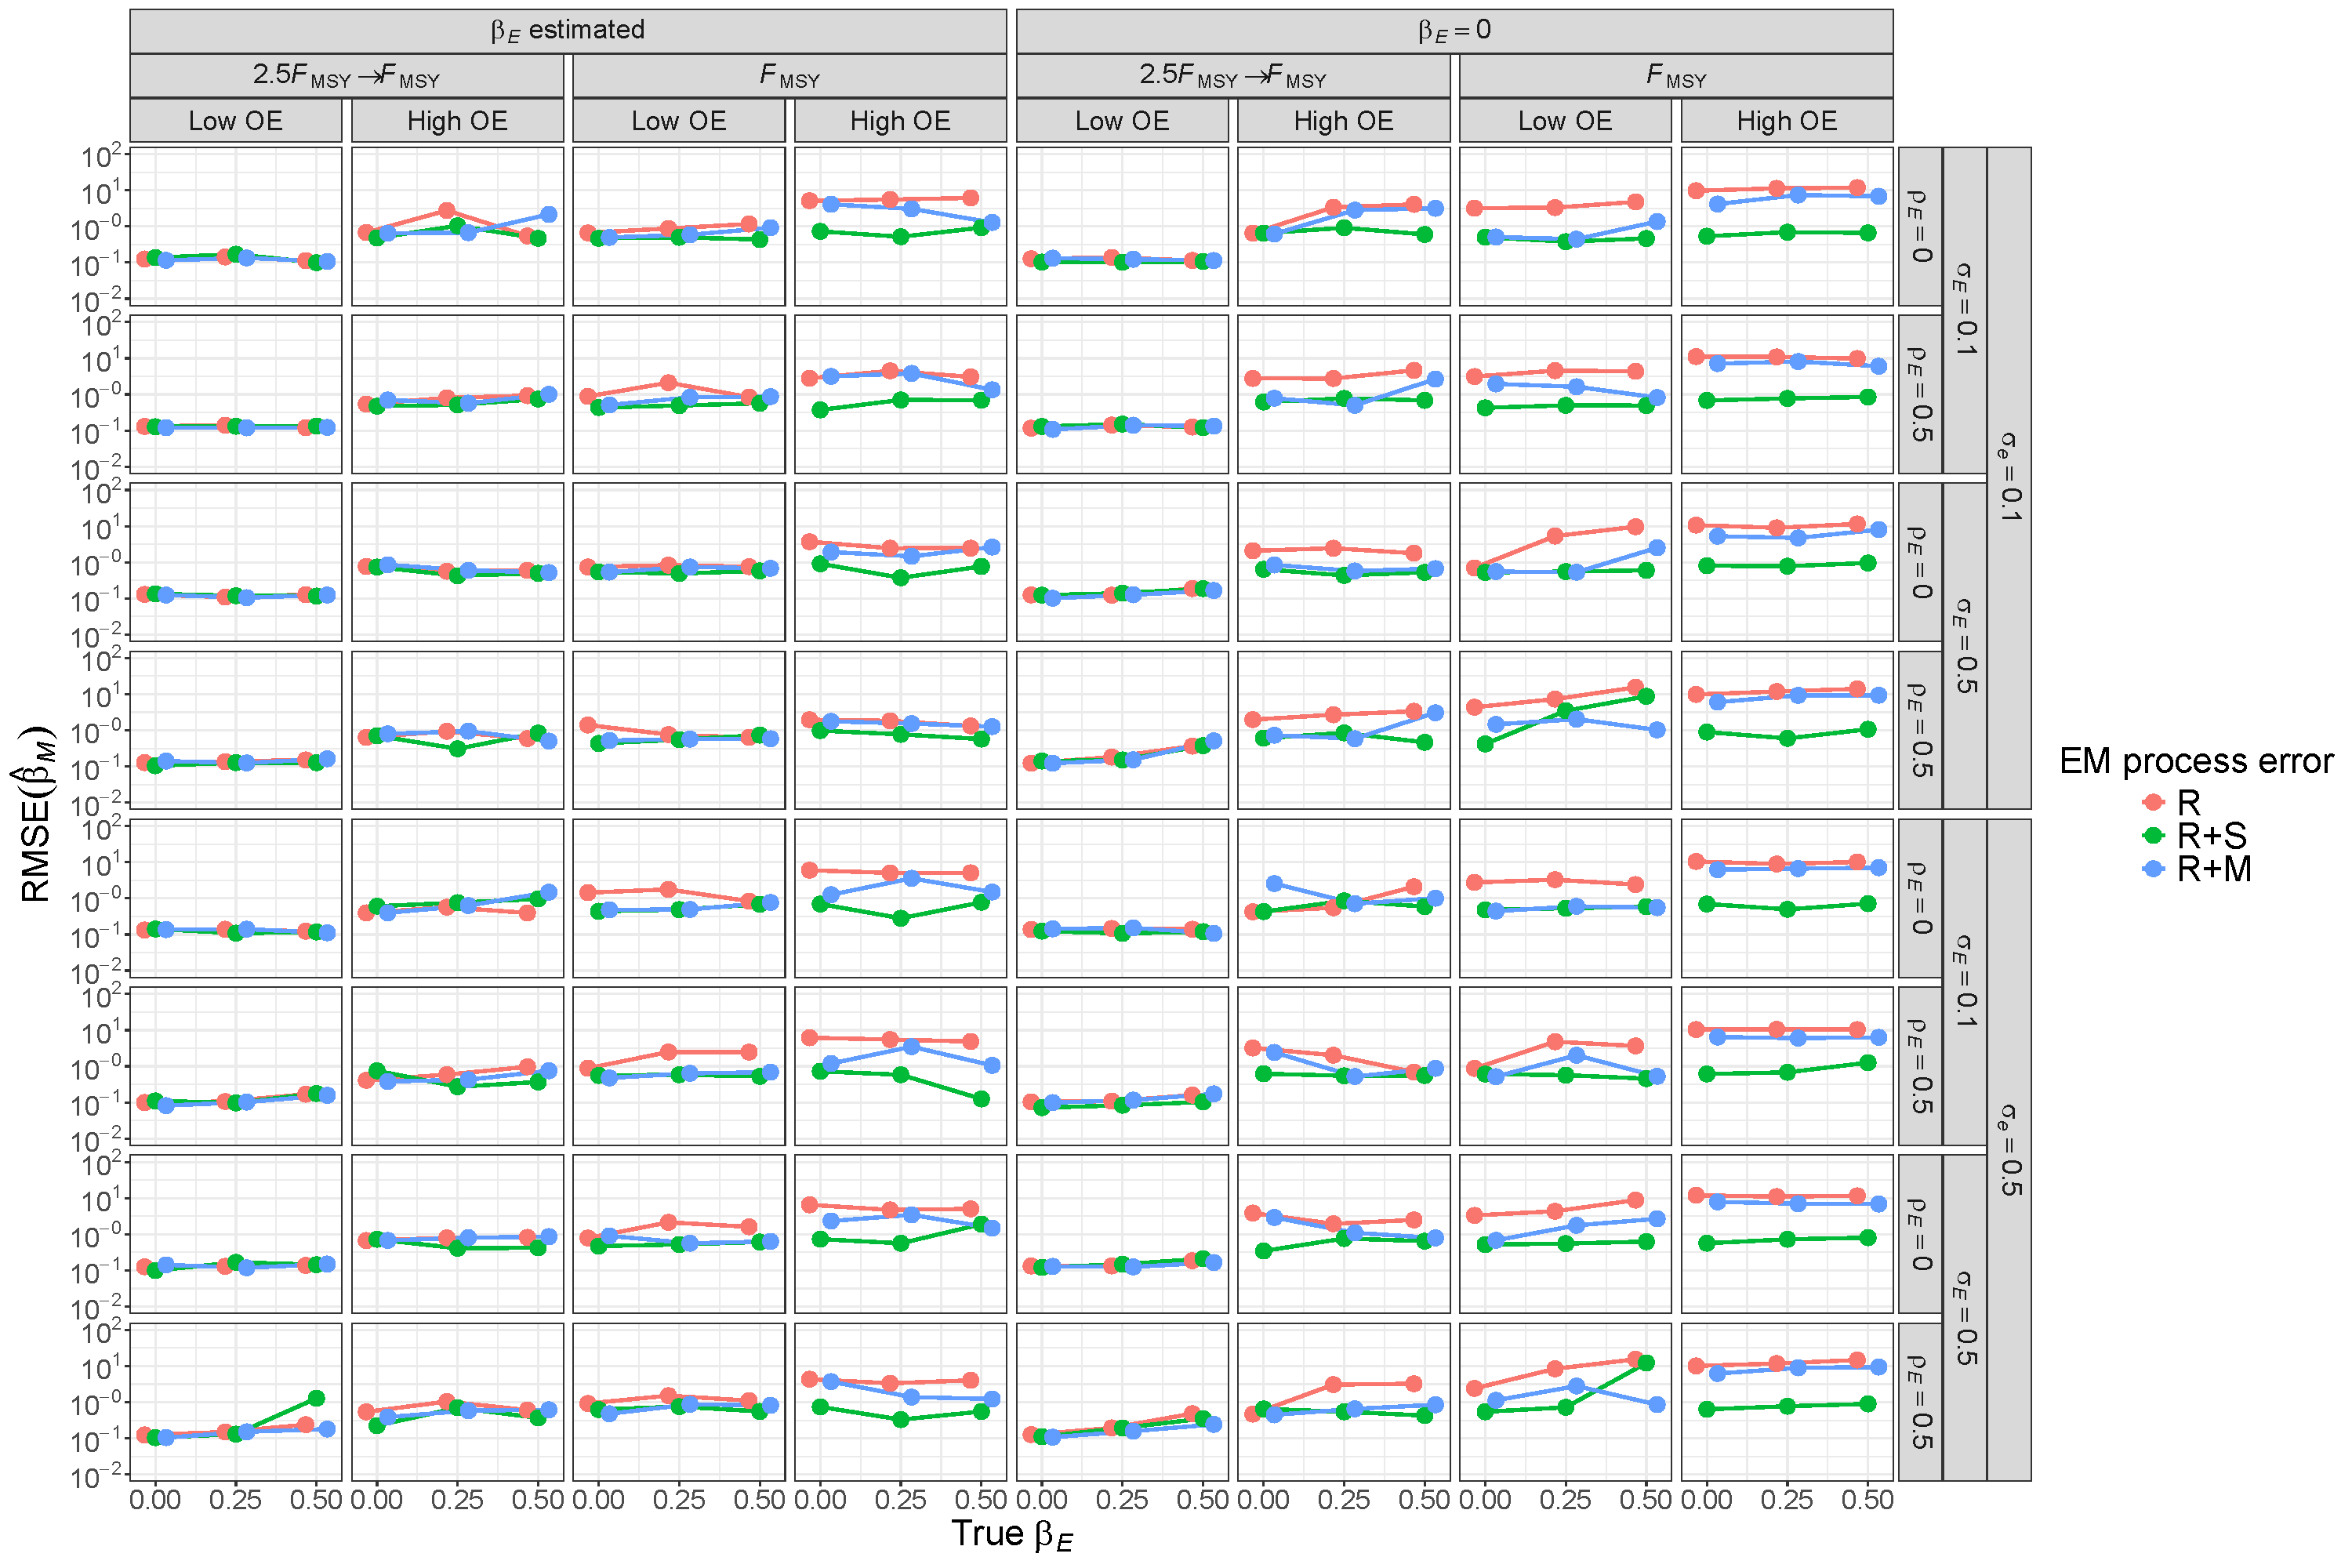
\includegraphics[height = \textheight]{beta_M_rmse_Rom}
\end{center}
\caption{For R OMs, \DIFdelbeginFL \DIFdelFL{root mean square error (}\DIFdelendFL RMSE \DIFdelbeginFL \DIFdelFL{) }\DIFdelendFL of estimates of  $\beta_M$ from fitting EMs with alternative process error assumptions and treatment of covariate effect ($\beta_E = 0$ or estimated).}\label{beta_M_rmse_Rom}
\end{figure}
\end{landscape}

\begin{landscape}
\begin{figure}
\begin{center}
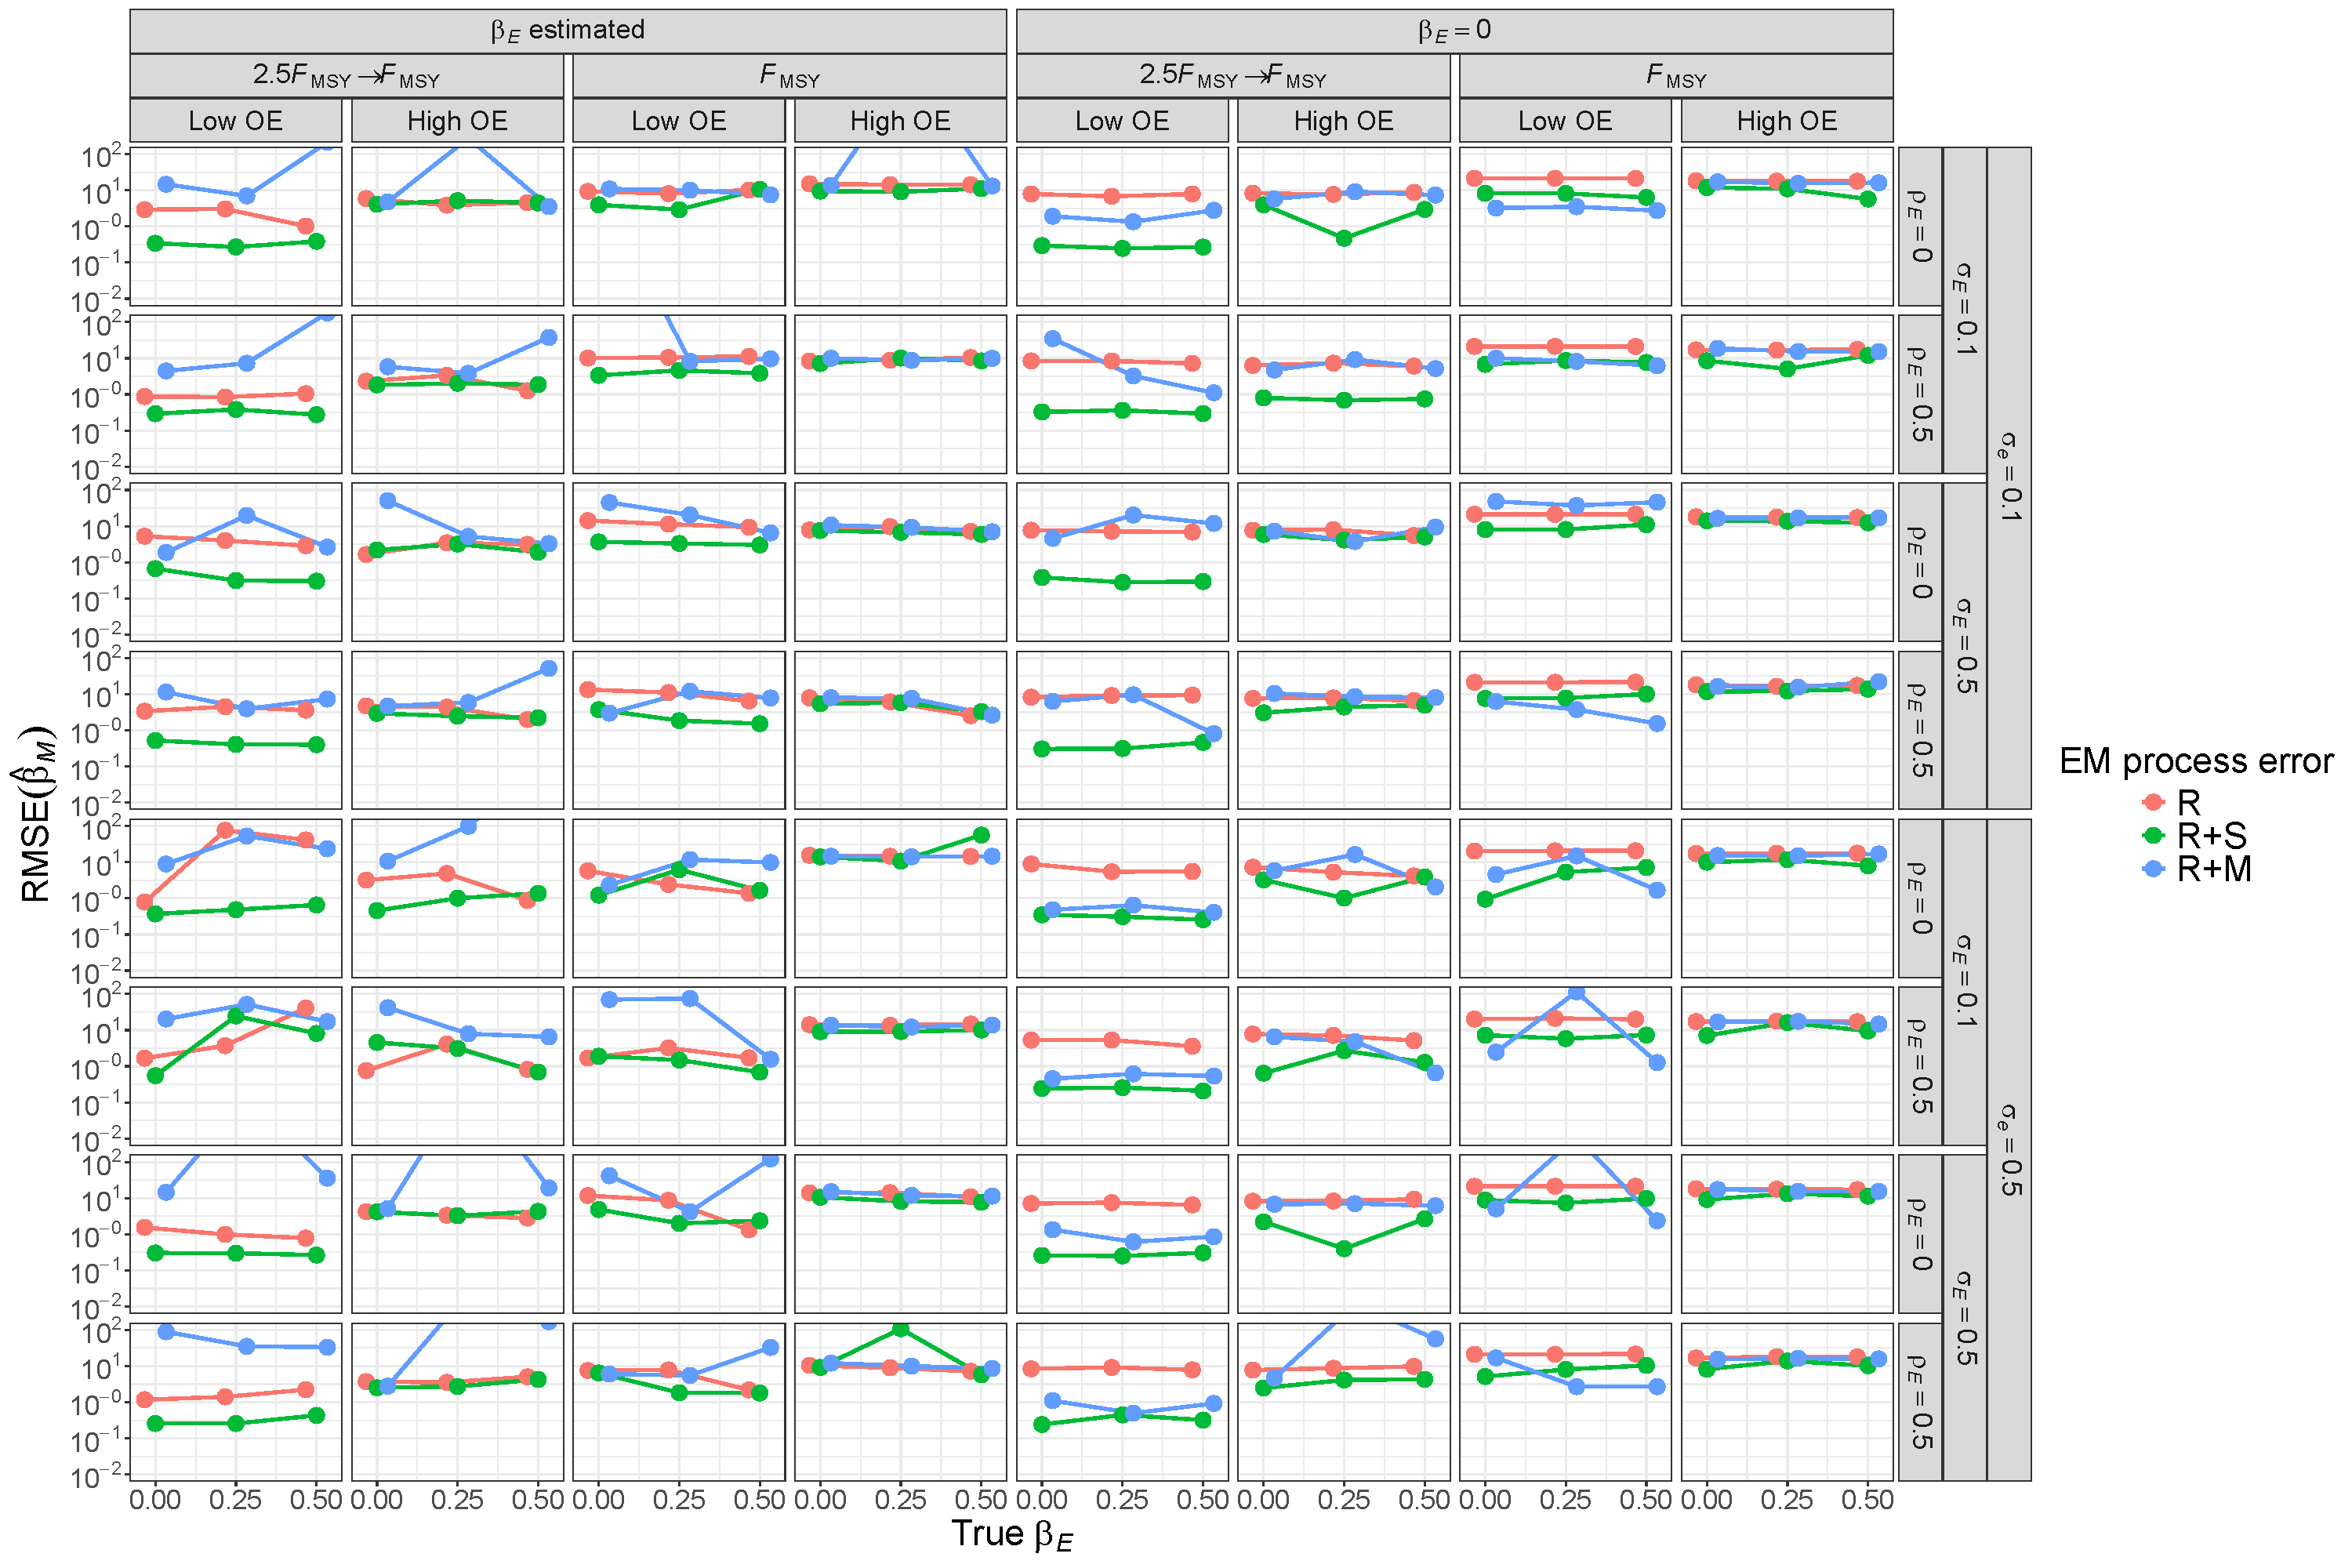
\includegraphics[height = \textheight]{beta_M_rmse_RSom}
\end{center}
\caption{For R+S OMs, \DIFdelbeginFL \DIFdelFL{root mean square error (}\DIFdelendFL RMSE \DIFdelbeginFL \DIFdelFL{) }\DIFdelendFL of estimates of  $\beta_M$ from fitting EMs with alternative process error assumptions and treatment of covariate effect ($\beta_E = 0$ or estimated).}\label{beta_M_rmse_RSom}
\end{figure}
\end{landscape}

\begin{landscape}
\begin{figure}
\begin{center}
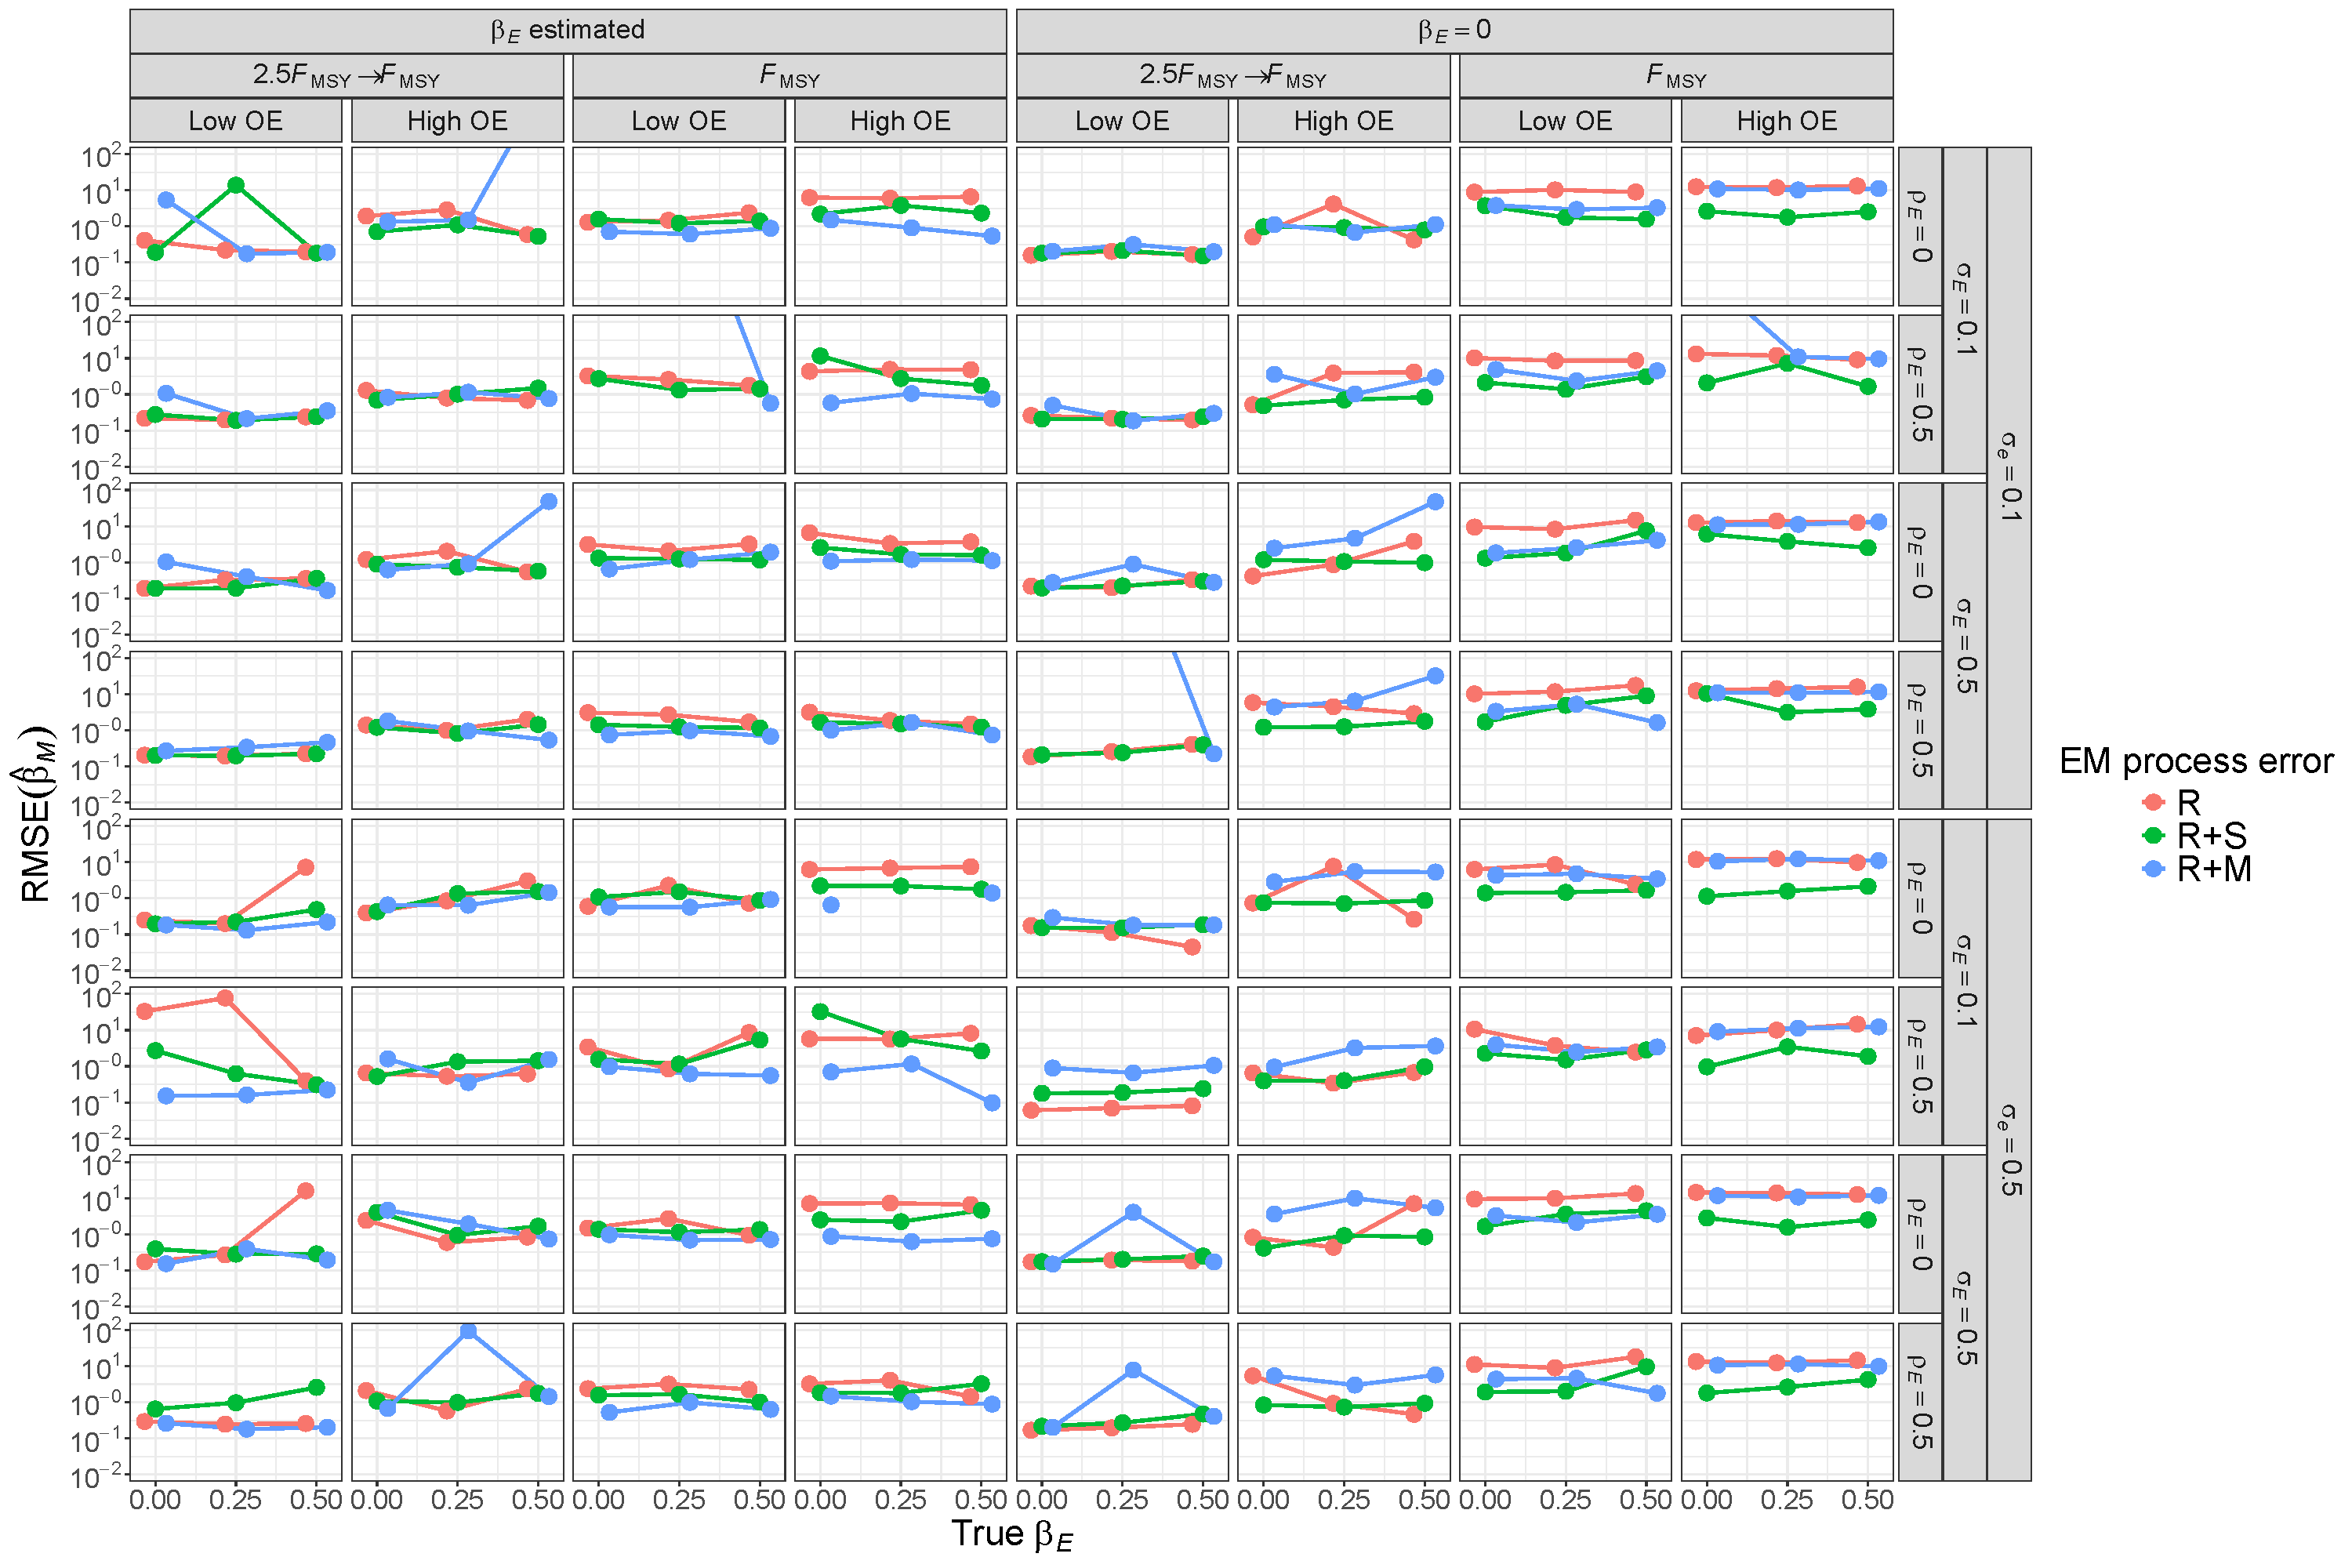
\includegraphics[height = \textheight]{beta_M_rmse_RMom}
\end{center}
\caption{For R+M OMs, \DIFdelbeginFL \DIFdelFL{root mean square error (}\DIFdelendFL RMSE \DIFdelbeginFL \DIFdelFL{) }\DIFdelendFL of estimates of  $\beta_M$ from fitting EMs with alternative process error assumptions and treatment of covariate effect ($\beta_E = 0$ or estimated).}\label{beta_M_rmse_RMom}
\end{figure}
\end{landscape}

\DIFdelbegin %DIFDELCMD < \hypertarget{terminal-year-natural-mortality-bias}{%
%DIFDELCMD < \subsection*{Terminal year natural mortality bias}\label{terminal-year-natural-mortality-bias}}
%DIFDELCMD < %%%
\DIFdelend \DIFaddbegin \subsection*{\DIFadd{Terminal year natural mortality bias}}\label{terminal-year-natural-mortality-bias}
\DIFaddend \addcontentsline{toc}{subsection}{Terminal year natural mortality bias}

\begin{landscape}
\begin{figure}
\begin{center}
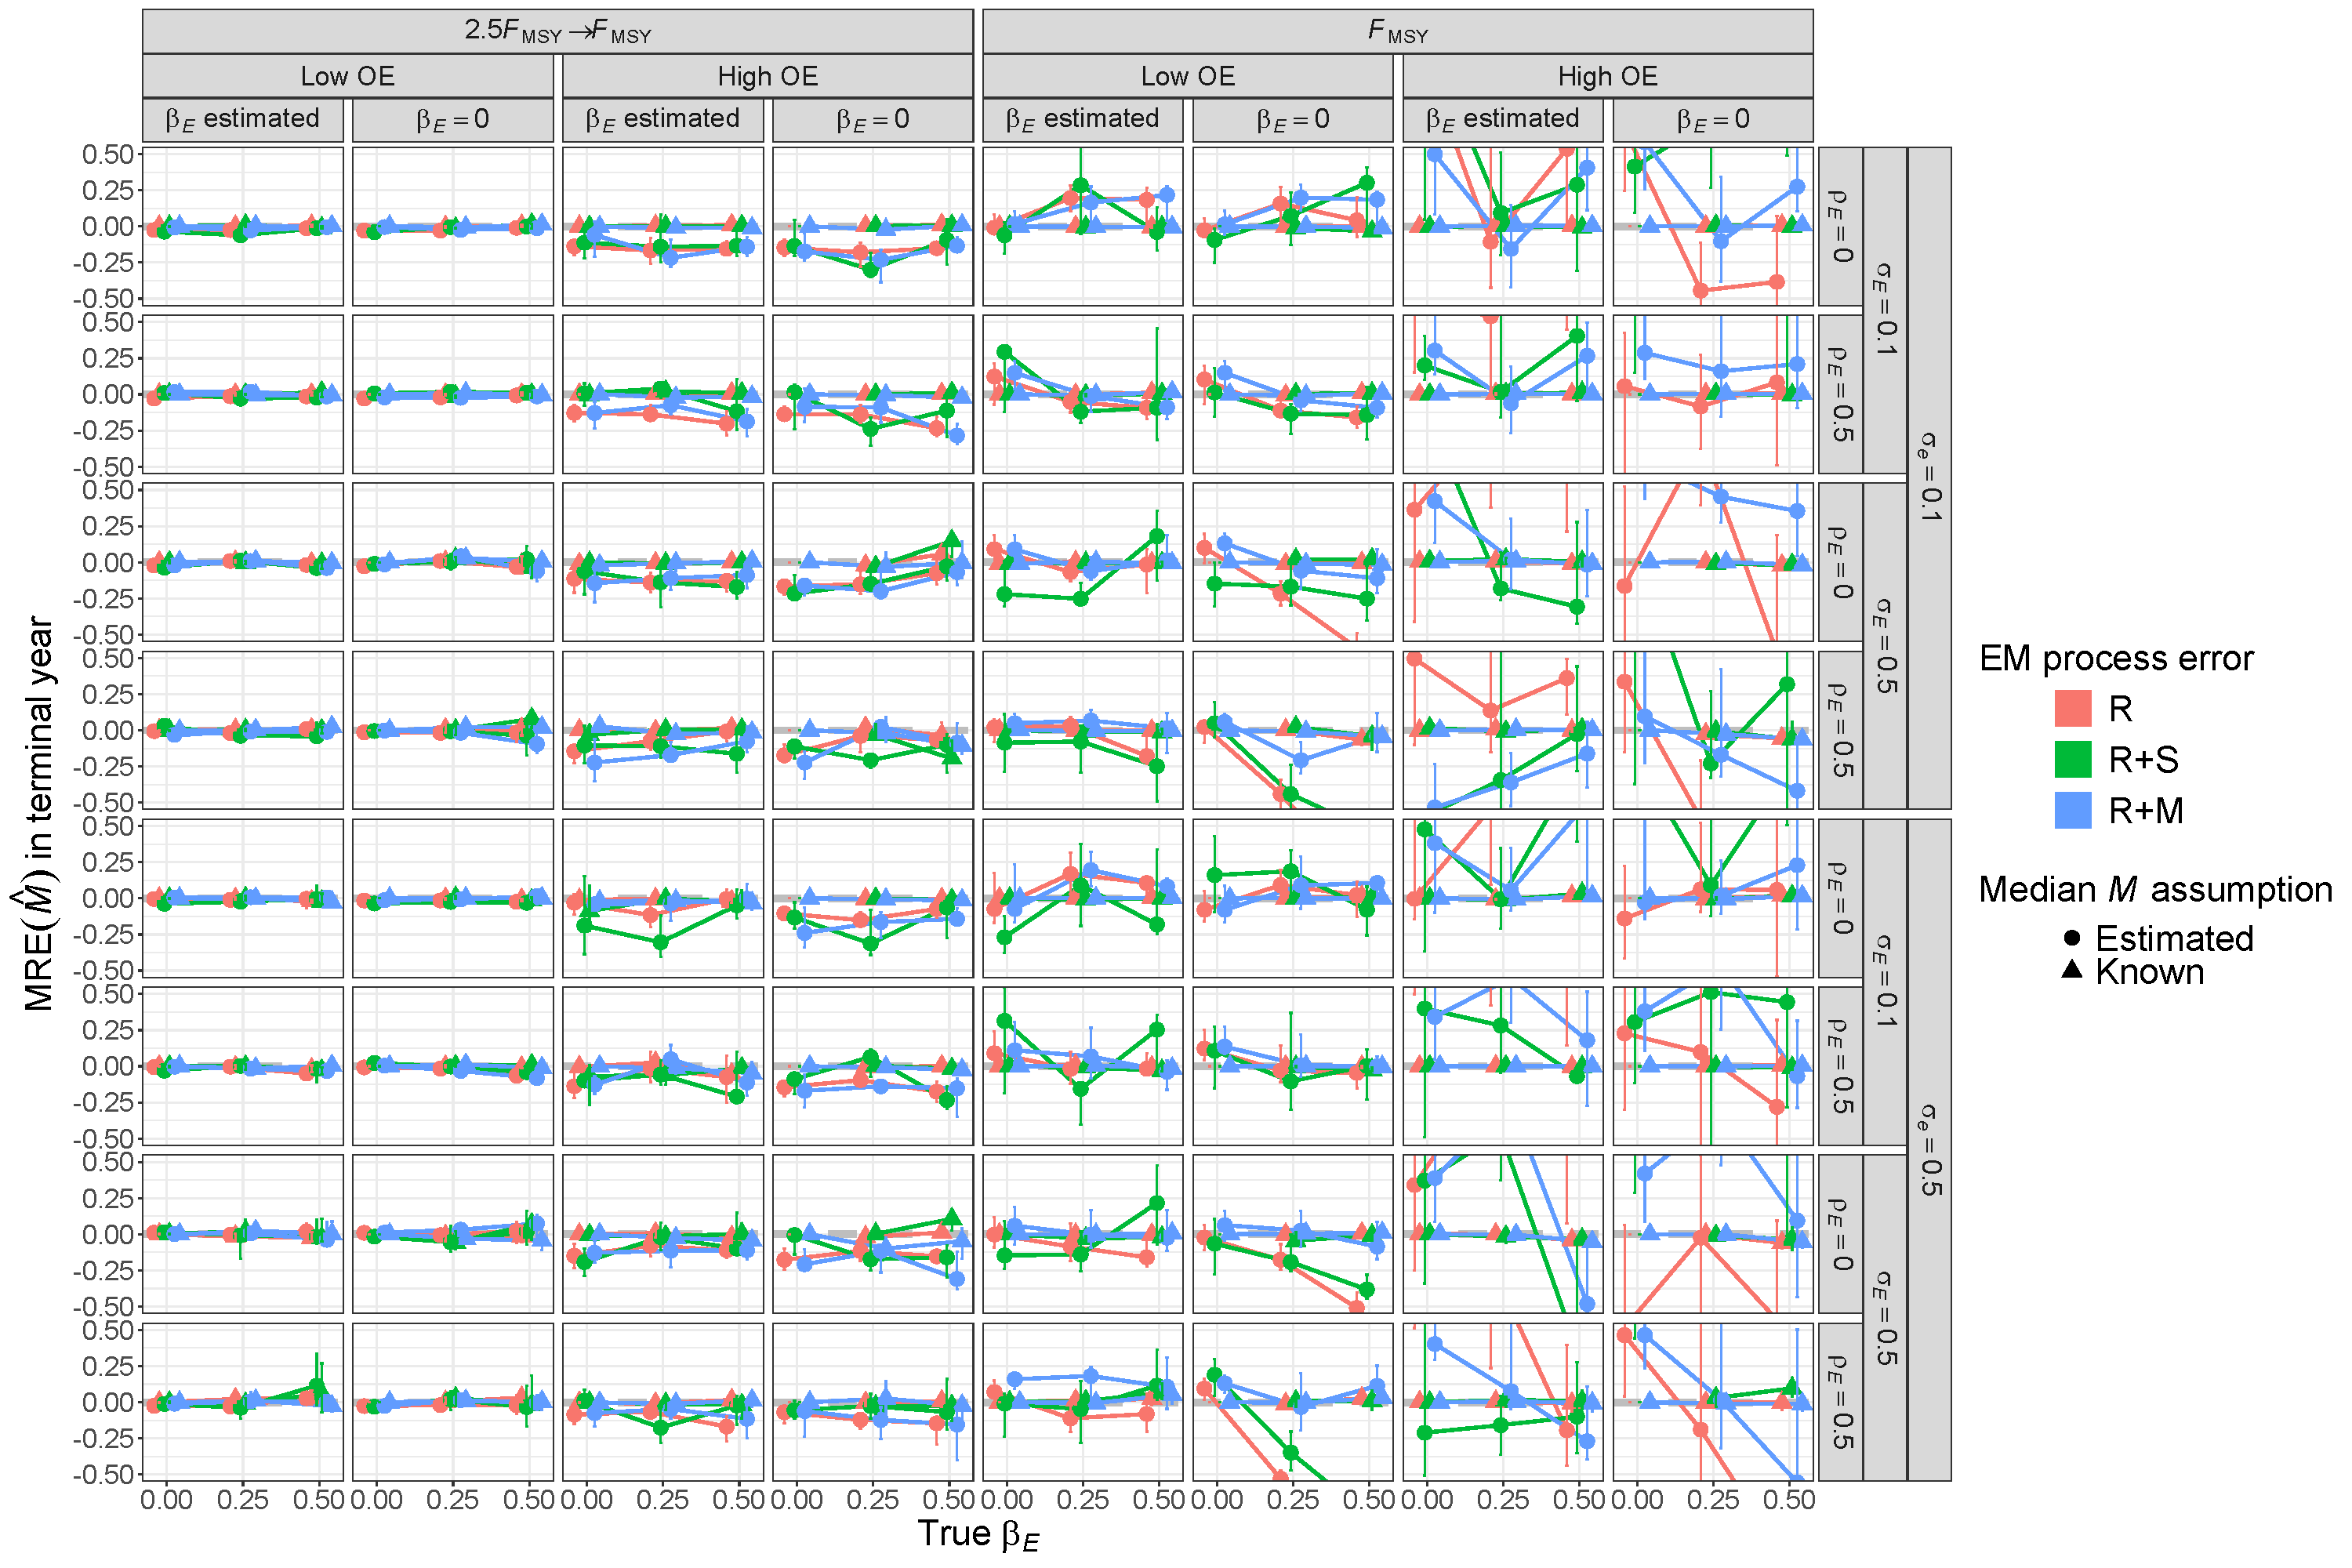
\includegraphics[height = \textheight]{terminal_year_M_bias_Rom}
\end{center}
\caption{For R OMs, median relative error (MRE) of estimates of \DIFdelbeginFL \DIFdelFL{natural mortality rate in the }\DIFdelendFL terminal year \DIFaddbeginFL \DIFaddFL{$M$ }\DIFaddendFL for EMs with alternative process error assumptions, treatment of covariate effect ($\beta_E = 0$ or estimated), and treatment of median \DIFdelbeginFL \DIFdelFL{natural mortality }\DIFdelendFL \DIFaddbeginFL \DIFaddFL{$M$ }\DIFaddendFL parameter ($\beta_M$ estimated or known).}\label{terminal_M_bias_Rom}
\end{figure}
\end{landscape}

\begin{landscape}
\begin{figure}
\begin{center}
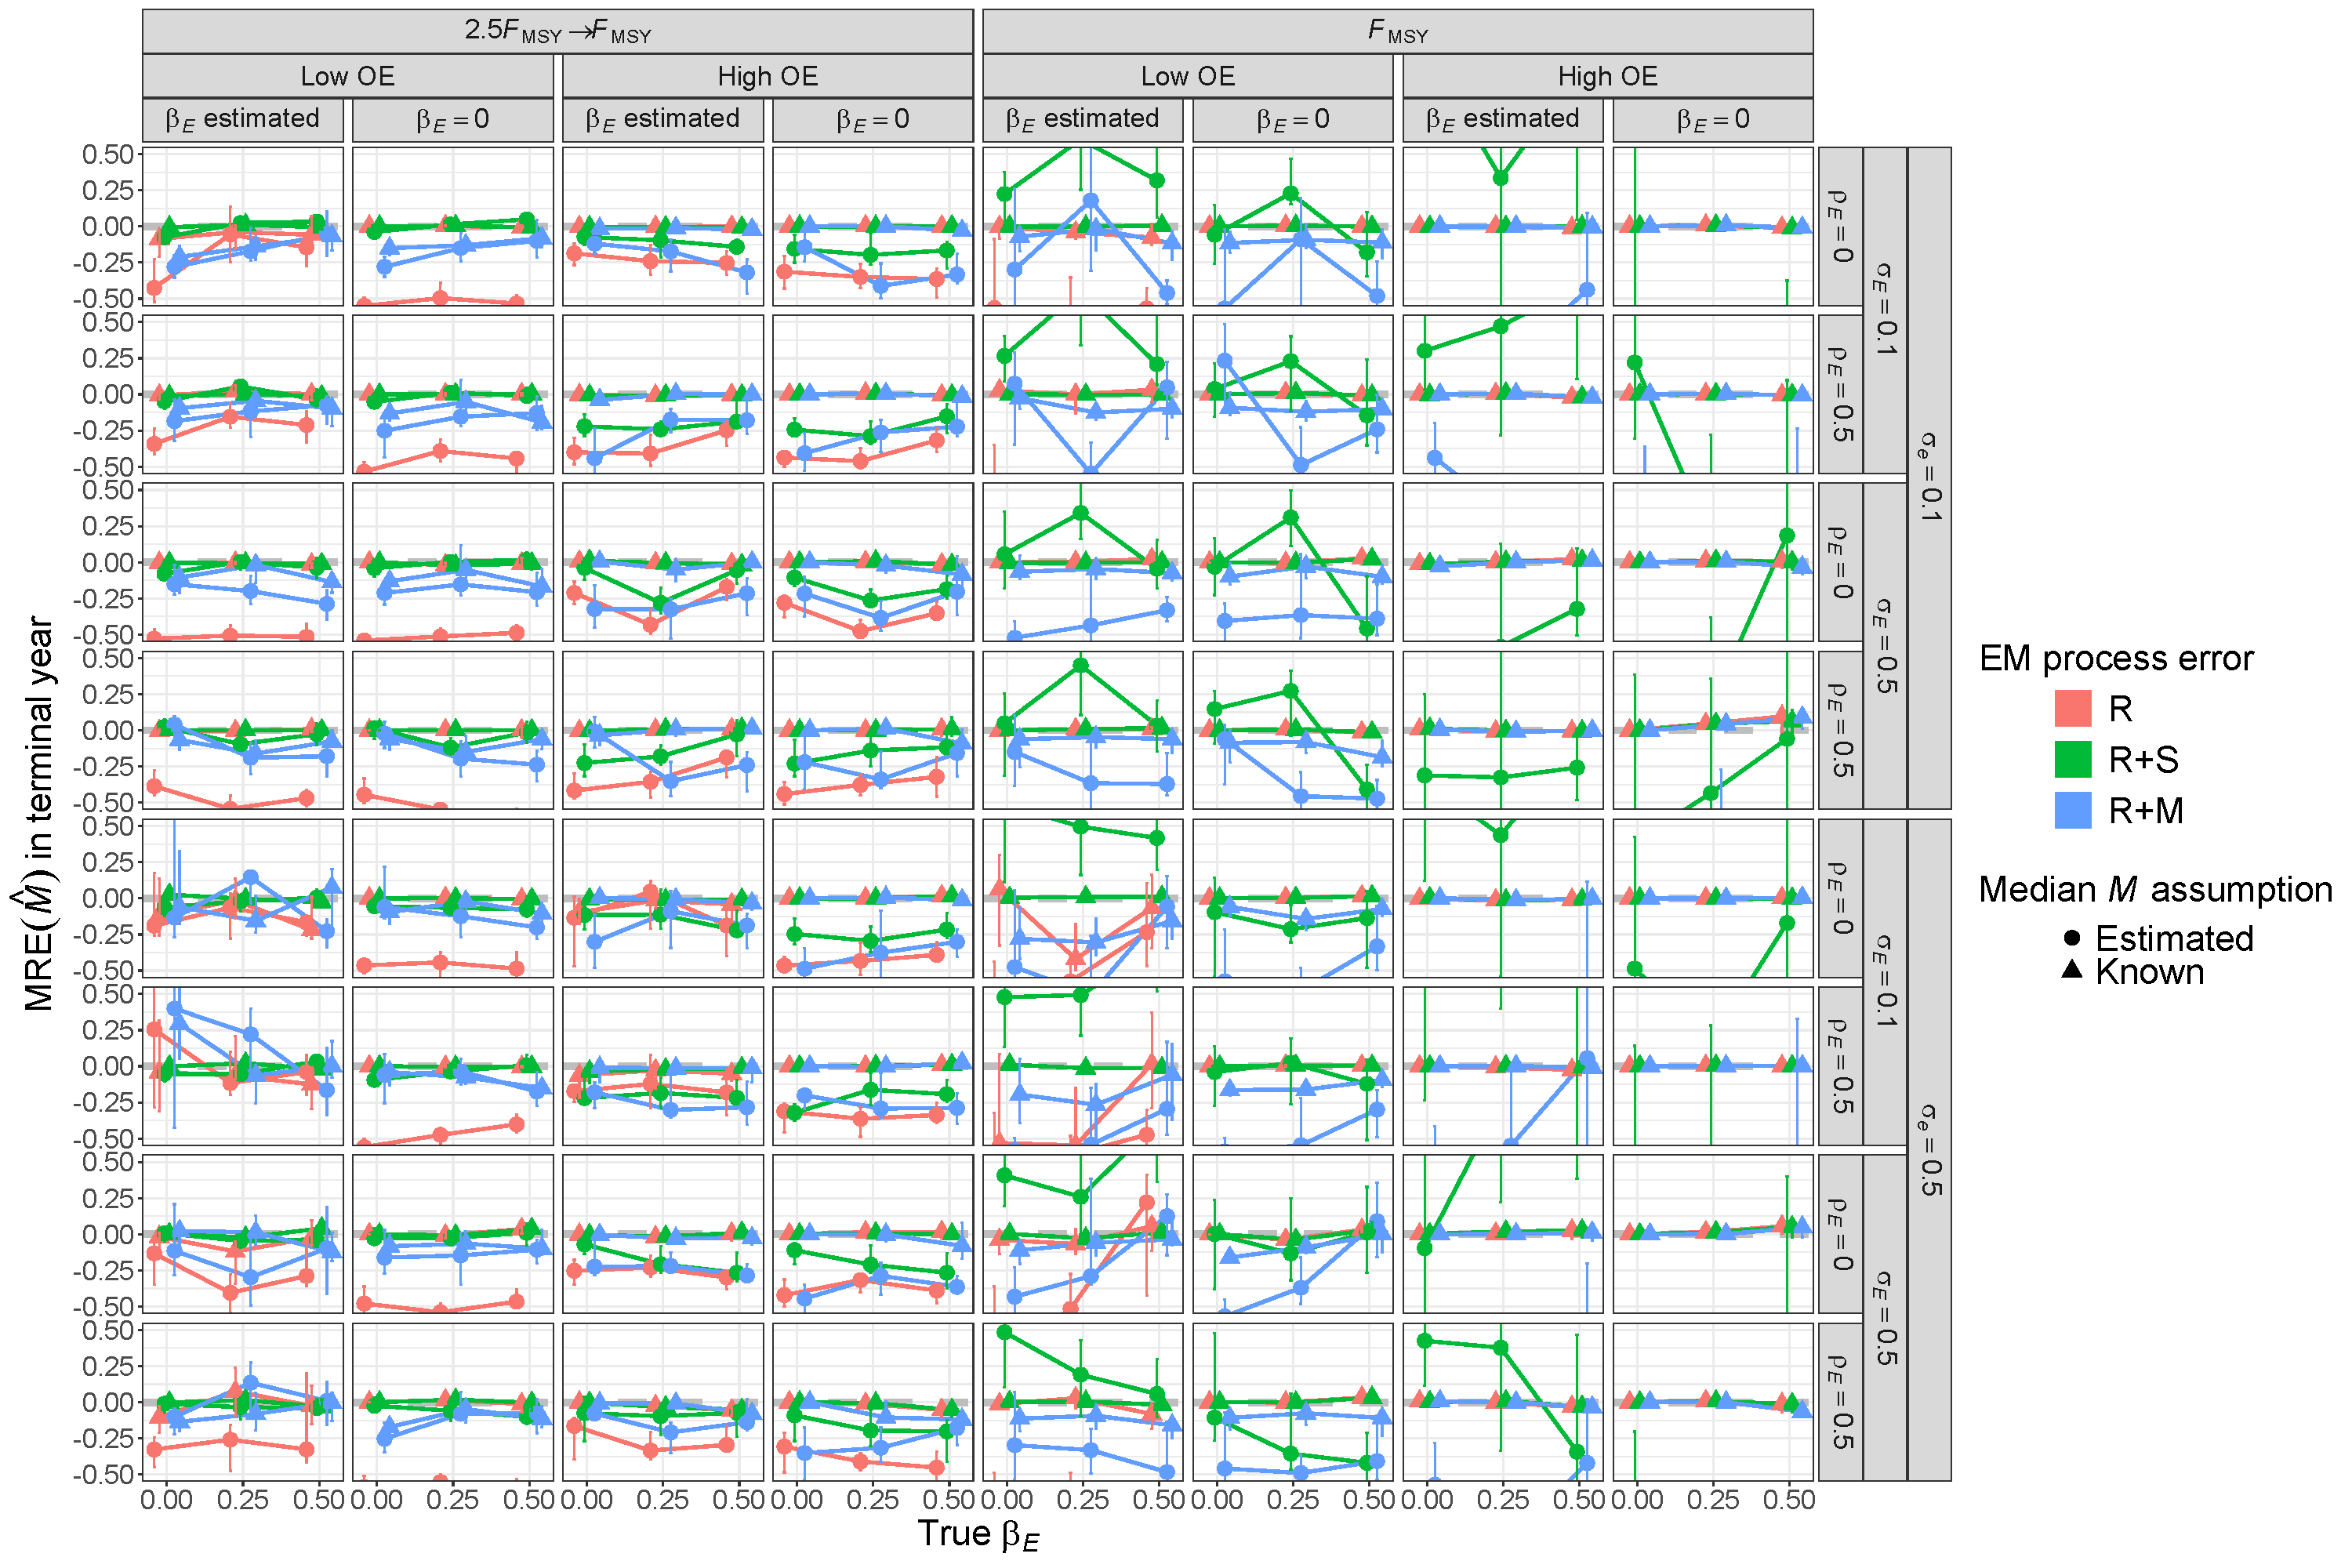
\includegraphics[height = \textheight]{terminal_year_M_bias_RSom}
\end{center}
\caption{For R+S OMs, median relative error (MRE) of estimates of \DIFdelbeginFL \DIFdelFL{natural mortality rate in the }\DIFdelendFL terminal year \DIFaddbeginFL \DIFaddFL{$M$ }\DIFaddendFL for EMs with alternative process error assumptions, treatment of covariate effect ($\beta_E = 0$ or estimated), and treatment of median \DIFdelbeginFL \DIFdelFL{natural mortality }\DIFdelendFL \DIFaddbeginFL \DIFaddFL{$M$ }\DIFaddendFL parameter ($\beta_M$ estimated or known).}\label{terminal_M_bias_RSom}
\end{figure}
\end{landscape}

\begin{landscape}
\begin{figure}
\begin{center}
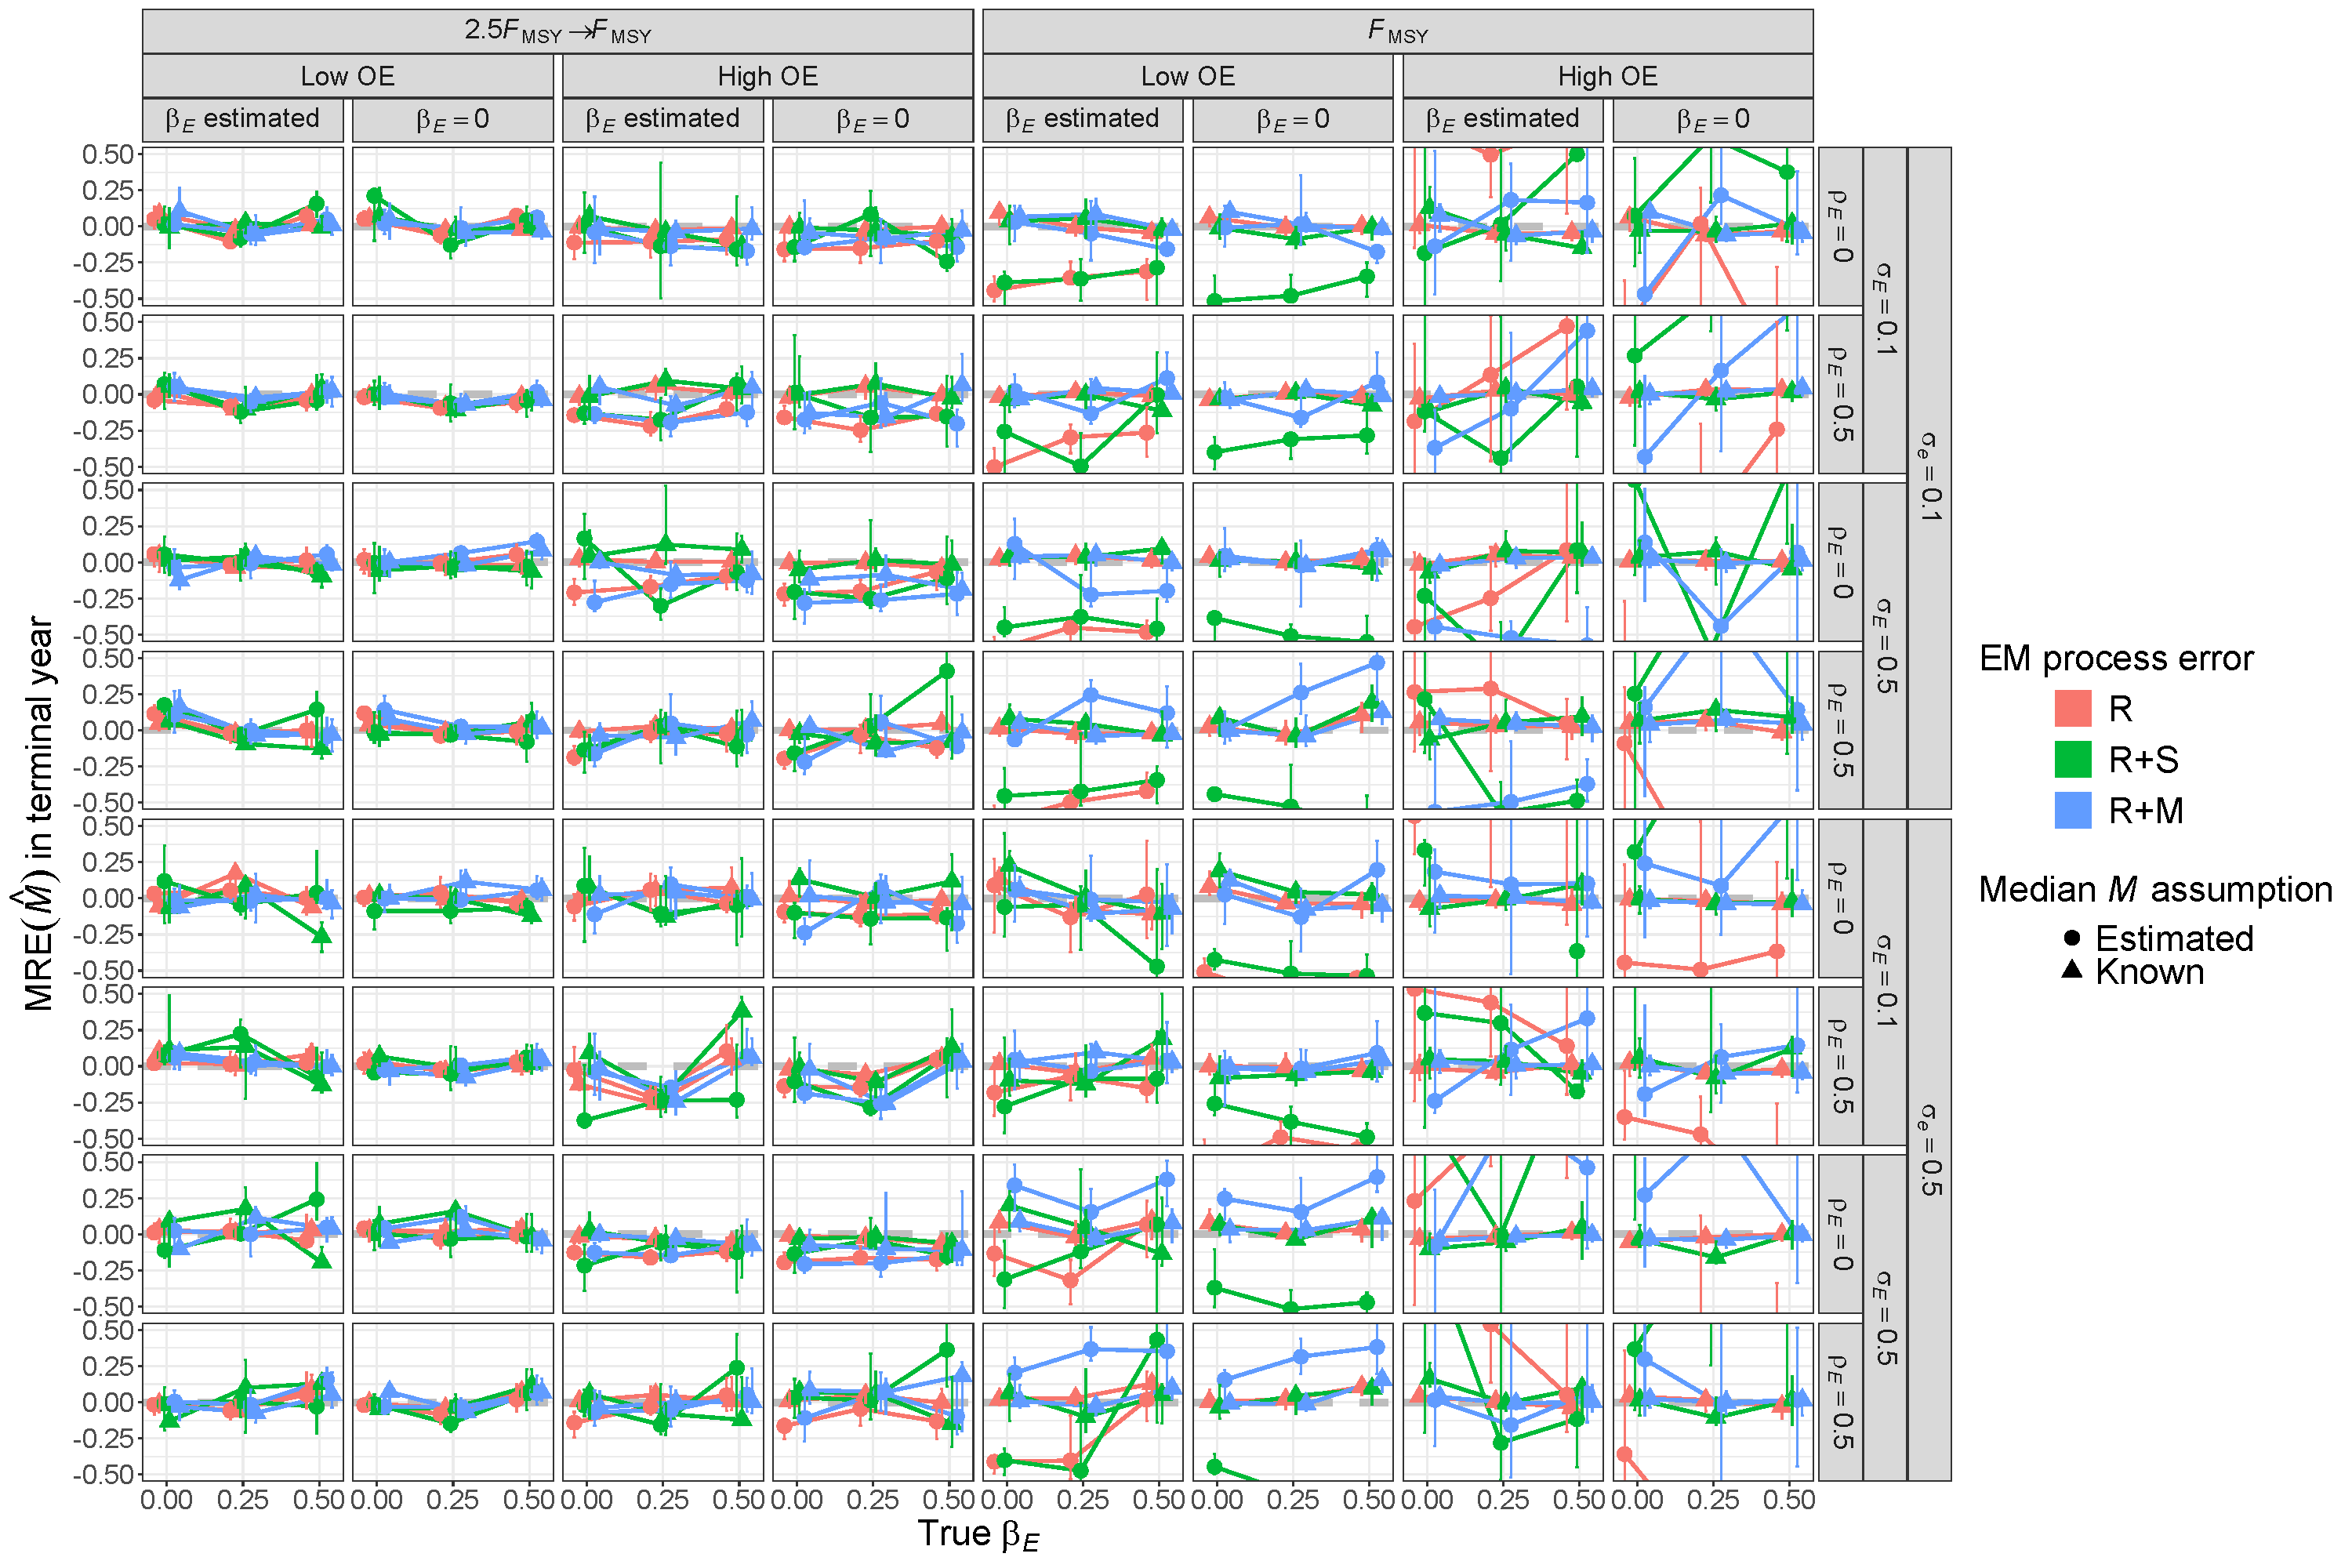
\includegraphics[height = \textheight]{terminal_year_M_bias_RMom}
\end{center}
\caption{For R+M OMs, median relative error (MRE) of estimates of \DIFdelbeginFL \DIFdelFL{natural mortality rate in the }\DIFdelendFL terminal year \DIFaddbeginFL \DIFaddFL{$M$ }\DIFaddendFL for EMs with alternative process error assumptions, treatment of covariate effect ($\beta_E = 0$ or estimated), and treatment of median \DIFdelbeginFL \DIFdelFL{natural mortality }\DIFdelendFL \DIFaddbeginFL \DIFaddFL{$M$ }\DIFaddendFL parameter ($\beta_M$ estimated or known).}\label{terminal_M_bias_RMom}
\end{figure}
\end{landscape}

\DIFdelbegin %DIFDELCMD < \hypertarget{terminal-year-natural-mortality-rmse}{%
%DIFDELCMD < \subsection*{Terminal year natural mortality RMSE}\label{terminal-year-natural-mortality-rmse}}
%DIFDELCMD < %%%
\DIFdelend \DIFaddbegin \subsection*{\DIFadd{Terminal year natural mortality accuracy}}\label{terminal-year-natural-mortality-accuracy}
\DIFaddend \addcontentsline{toc}{subsection}{Terminal year natural mortality \DIFdelbegin \DIFdel{RMSE}\DIFdelend \DIFaddbegin \DIFadd{accuracy}\DIFaddend }

\begin{landscape}
\begin{figure}
\begin{center}
\DIFdelbeginFL %DIFDELCMD < 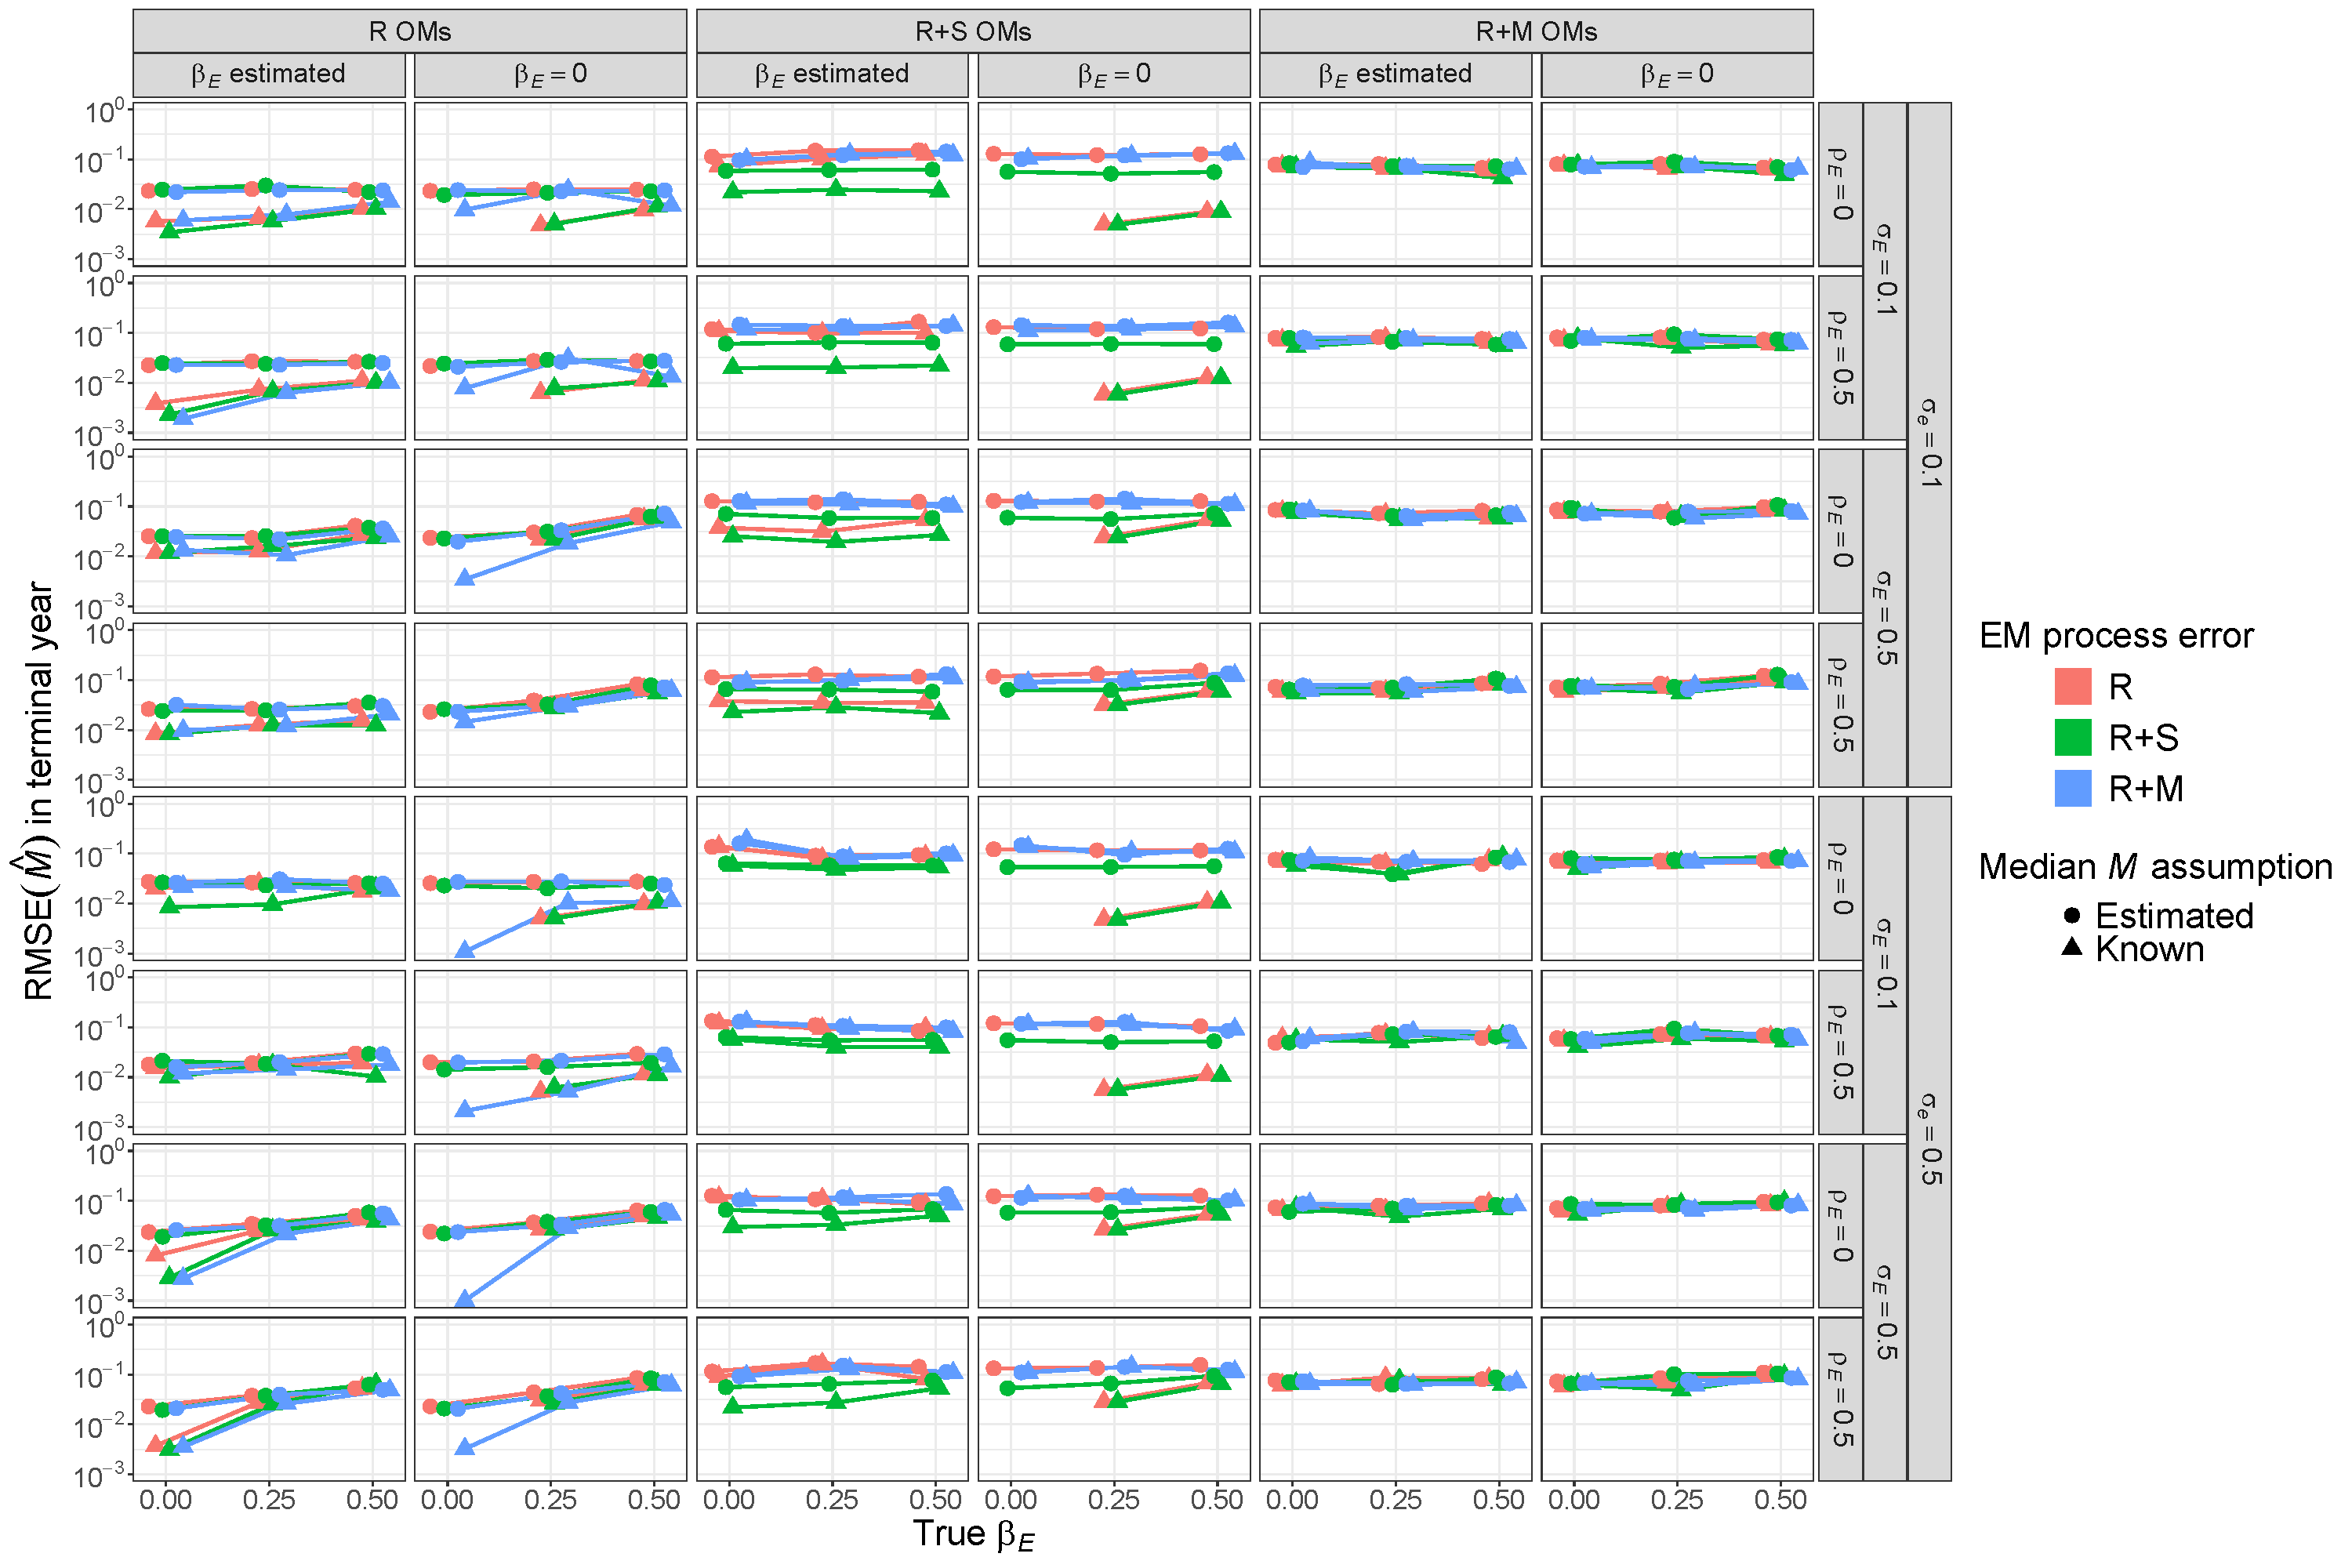
\includegraphics[height = \textheight]{terminal_year_M_rmse_main}
%DIFDELCMD < %%%
\DIFdelendFL \DIFaddbeginFL 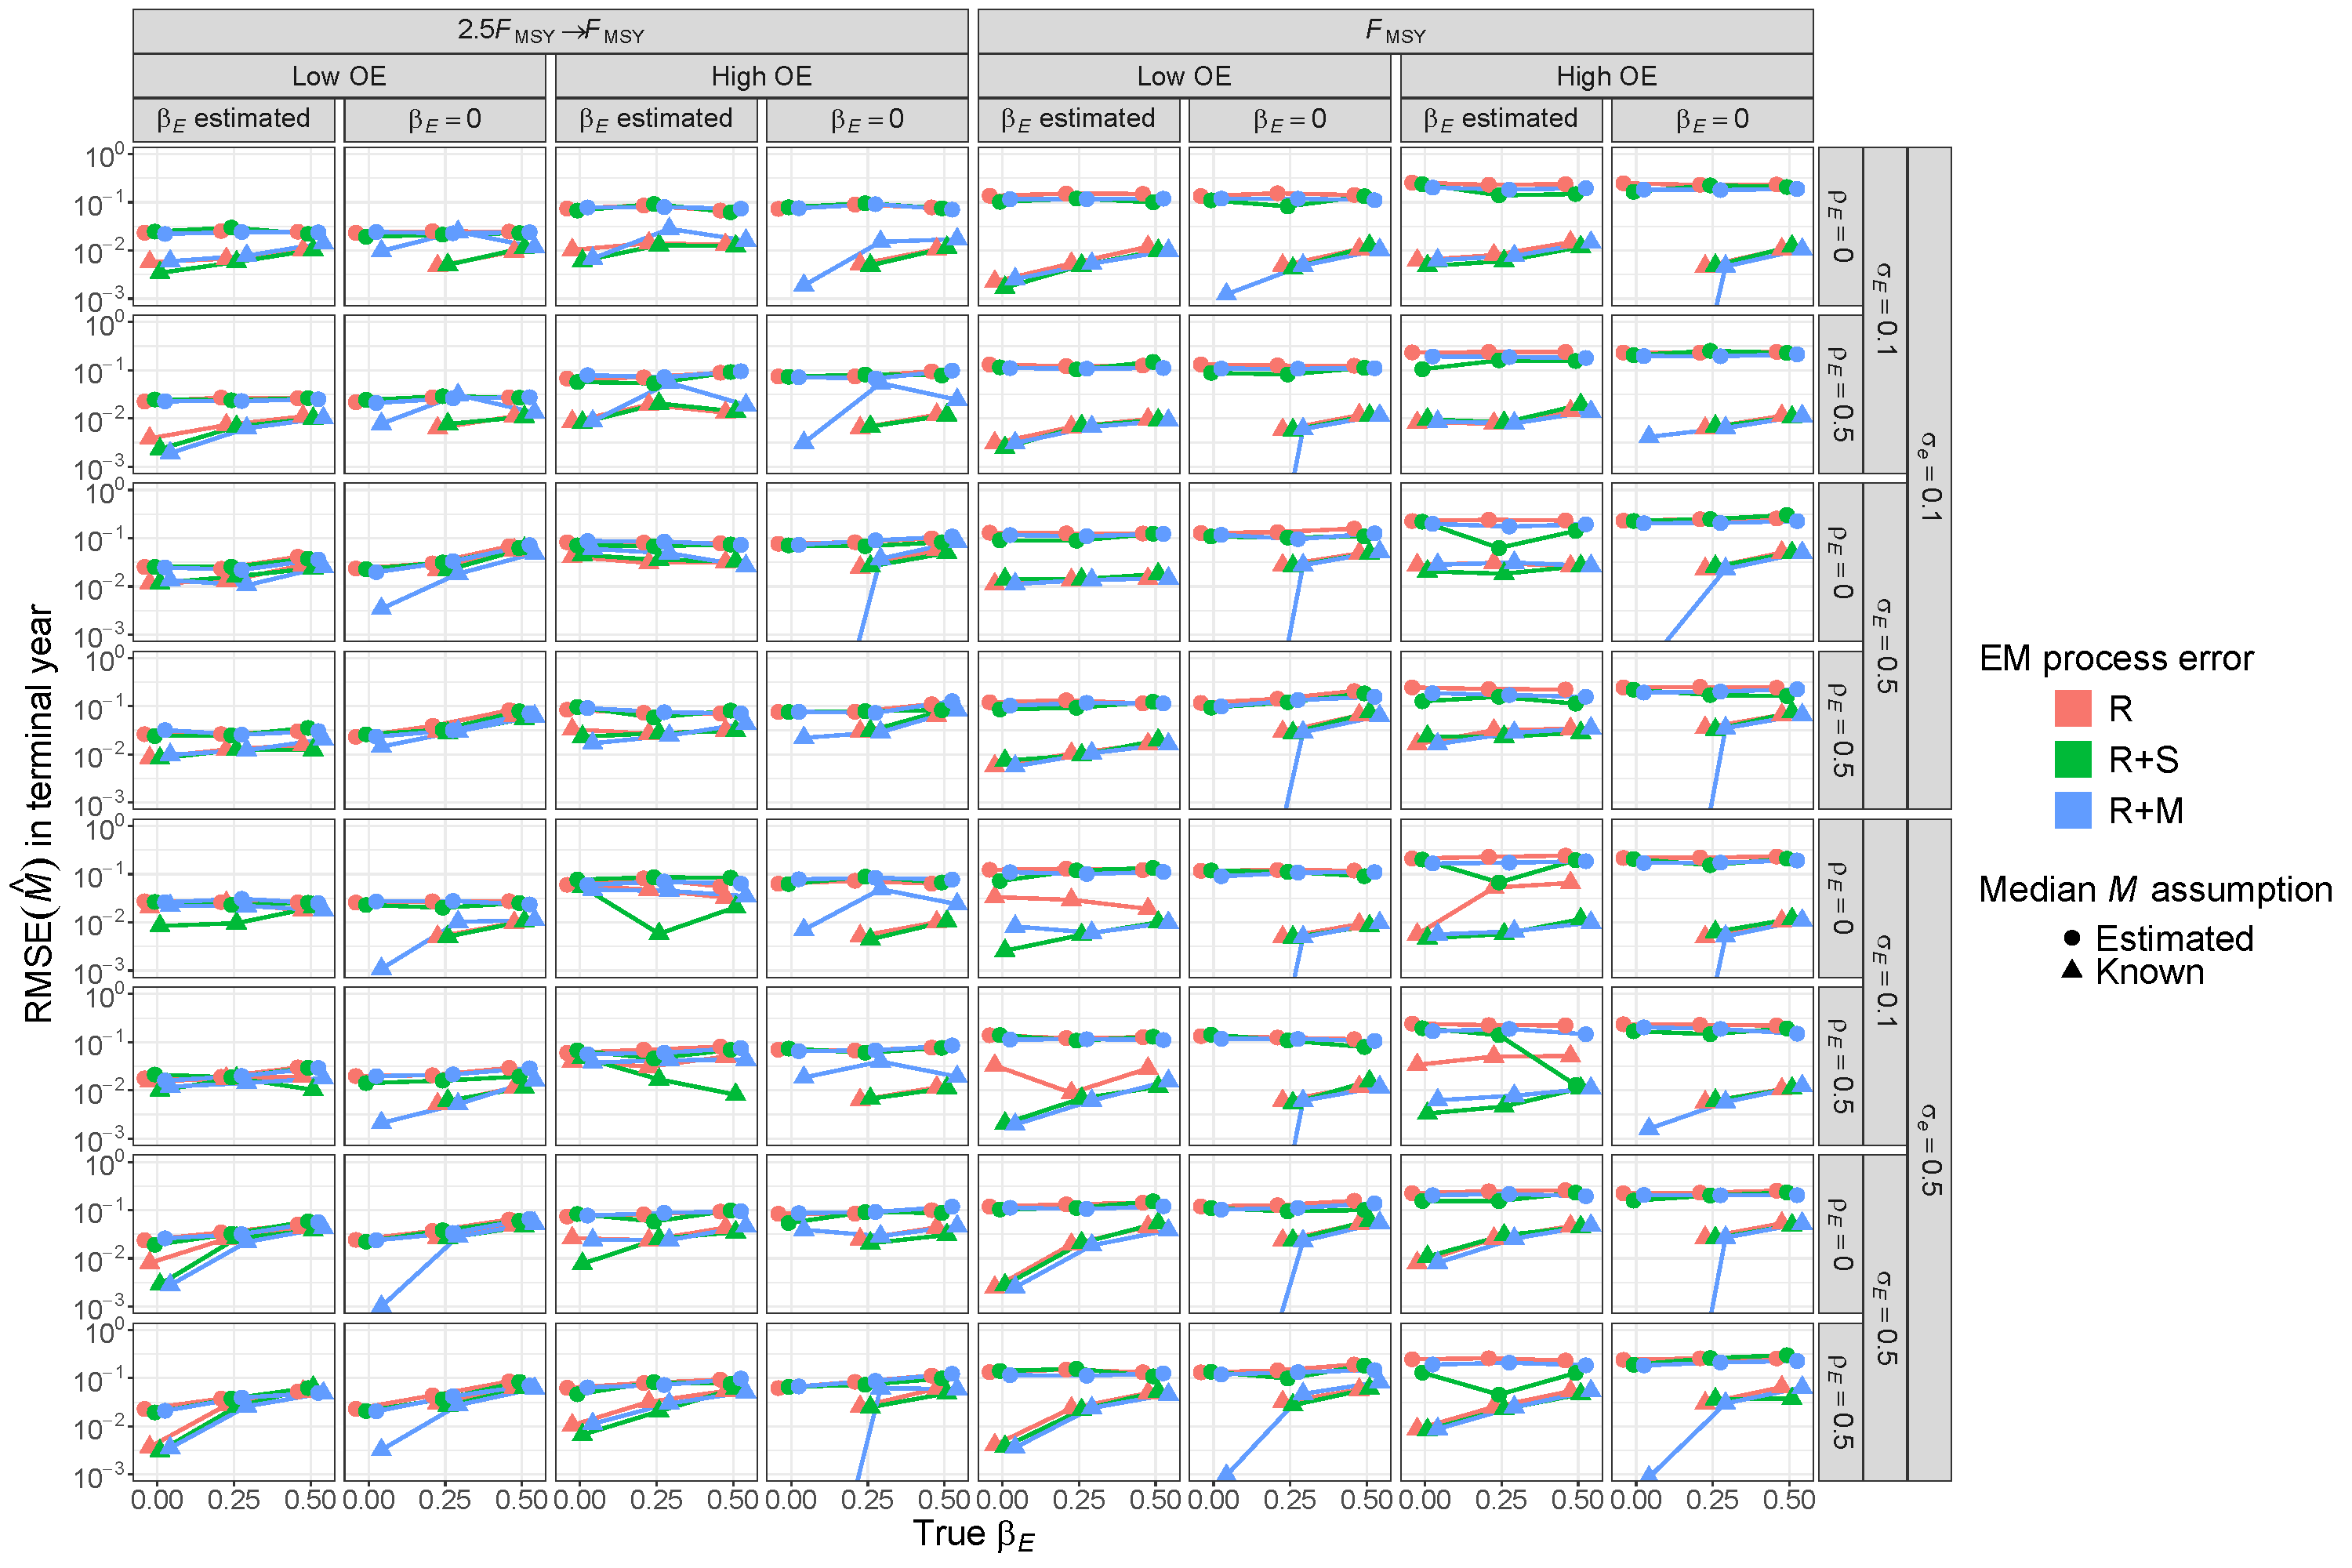
\includegraphics[height = \textheight]{terminal_year_M_rmse_Rom}
\DIFaddendFL \end{center}
\caption{\DIFdelbeginFL \DIFdelFL{Root mean square error (}\DIFdelendFL \DIFaddbeginFL \DIFaddFL{For R OMs, }\DIFaddendFL RMSE \DIFdelbeginFL \DIFdelFL{) }\DIFdelendFL of estimates of \DIFdelbeginFL \DIFdelFL{natural mortality rate in the }\DIFdelendFL terminal year \DIFaddbeginFL \DIFaddFL{$M$ }\DIFaddendFL for EMs with alternative process error assumptions, treatment of covariate effect ($\beta_E = 0$ or estimated), and treatment of median \DIFdelbeginFL \DIFdelFL{natural mortality }\DIFdelendFL \DIFaddbeginFL \DIFaddFL{$M$ }\DIFaddendFL parameter ($\beta_M$ estimated or known).\DIFdelbeginFL \DIFdelFL{All OMs had low population observation error and contrast in fishing mortality.}\DIFdelendFL }\DIFdelbeginFL %DIFDELCMD < \label{terminal_M_rmse}
%DIFDELCMD < %%%
\DIFdelendFL \DIFaddbeginFL \label{terminal_M_rmse_Rom}
\DIFaddendFL \end{figure}
\end{landscape}

\begin{landscape}
\begin{figure}
\begin{center}
\DIFdelbeginFL %DIFDELCMD < 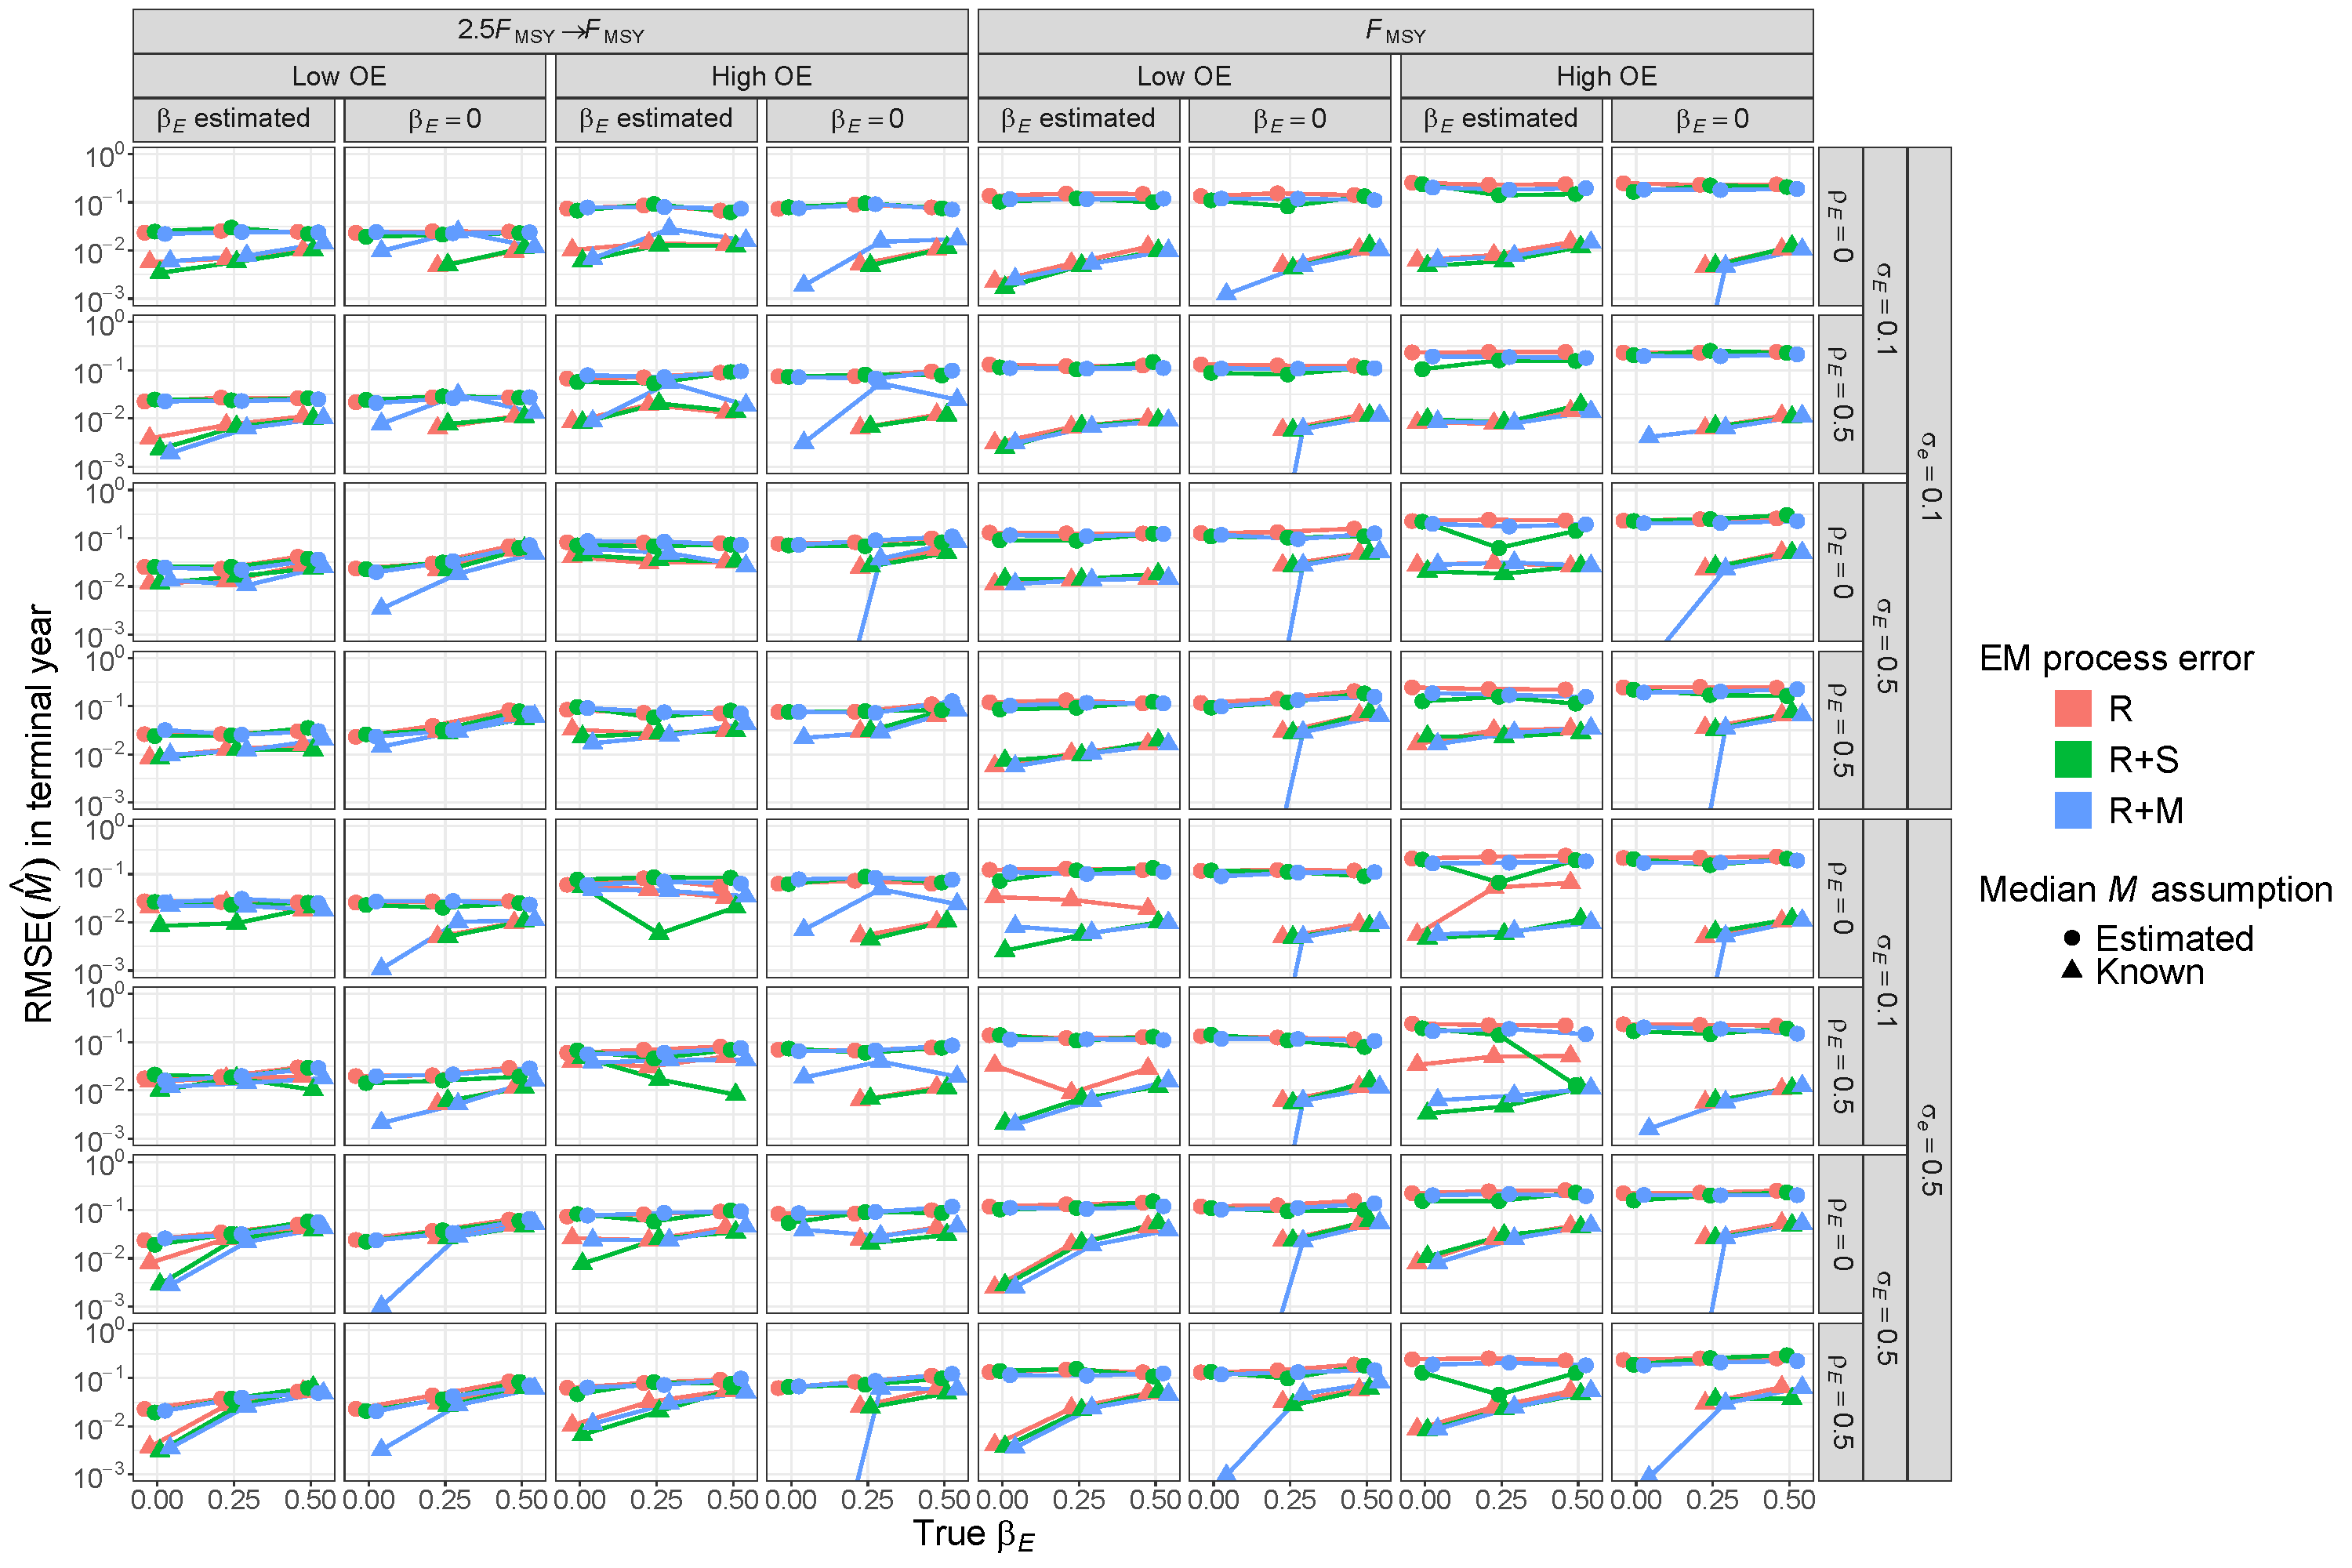
\includegraphics[height = \textheight]{terminal_year_M_rmse_Rom}
%DIFDELCMD < %%%
\DIFdelendFL \DIFaddbeginFL 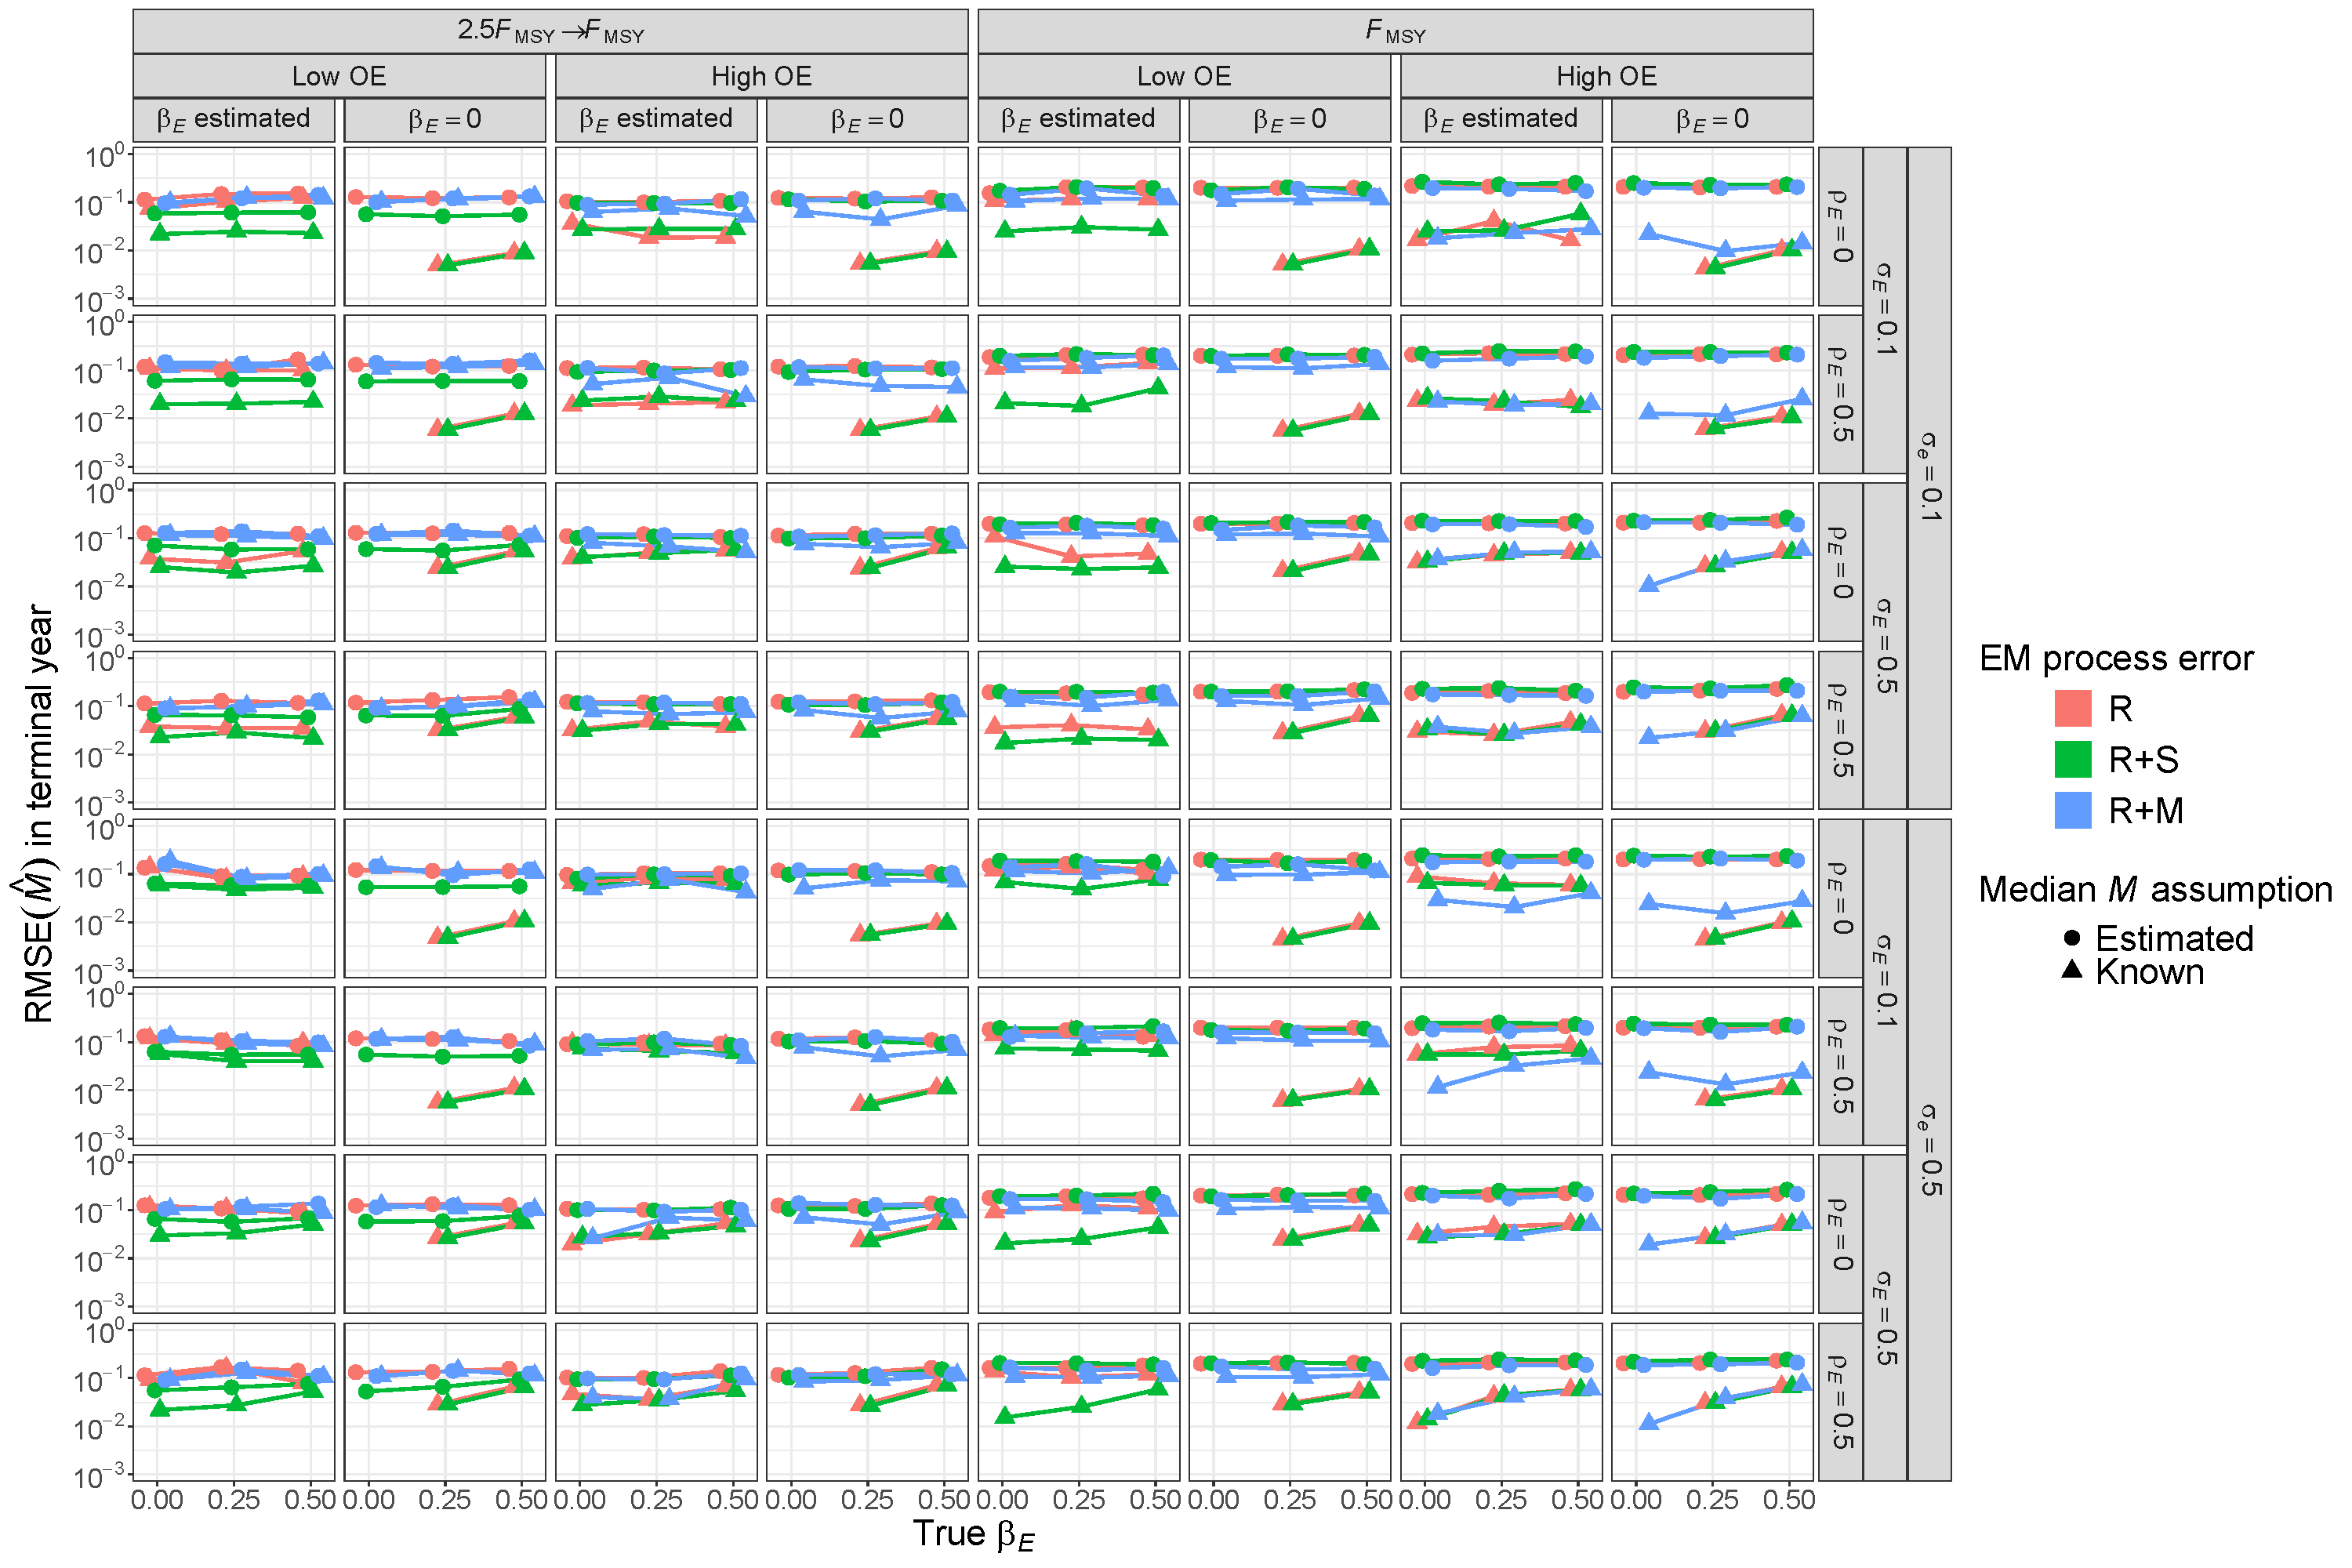
\includegraphics[height = \textheight]{terminal_year_M_rmse_RSom}
\DIFaddendFL \end{center}
\caption{For R\DIFaddbeginFL \DIFaddFL{+S }\DIFaddendFL OMs, \DIFdelbeginFL \DIFdelFL{root mean square error (}\DIFdelendFL RMSE \DIFdelbeginFL \DIFdelFL{) }\DIFdelendFL of estimates of \DIFdelbeginFL \DIFdelFL{natural mortality rate in the }\DIFdelendFL terminal year \DIFaddbeginFL \DIFaddFL{$M$ }\DIFaddendFL for EMs with alternative process error assumptions, treatment of covariate effect ($\beta_E = 0$ or estimated), and treatment of median \DIFdelbeginFL \DIFdelFL{natural mortality }\DIFdelendFL \DIFaddbeginFL \DIFaddFL{$M$ }\DIFaddendFL parameter ($\beta_M$ estimated or known).}\DIFdelbeginFL %DIFDELCMD < \label{terminal_M_rmse_Rom}
%DIFDELCMD < %%%
\DIFdelendFL \DIFaddbeginFL \label{terminal_M_rmse_RSom}
\DIFaddendFL \end{figure}
\end{landscape}

\begin{landscape}
\begin{figure}
\begin{center}
\DIFdelbeginFL %DIFDELCMD < 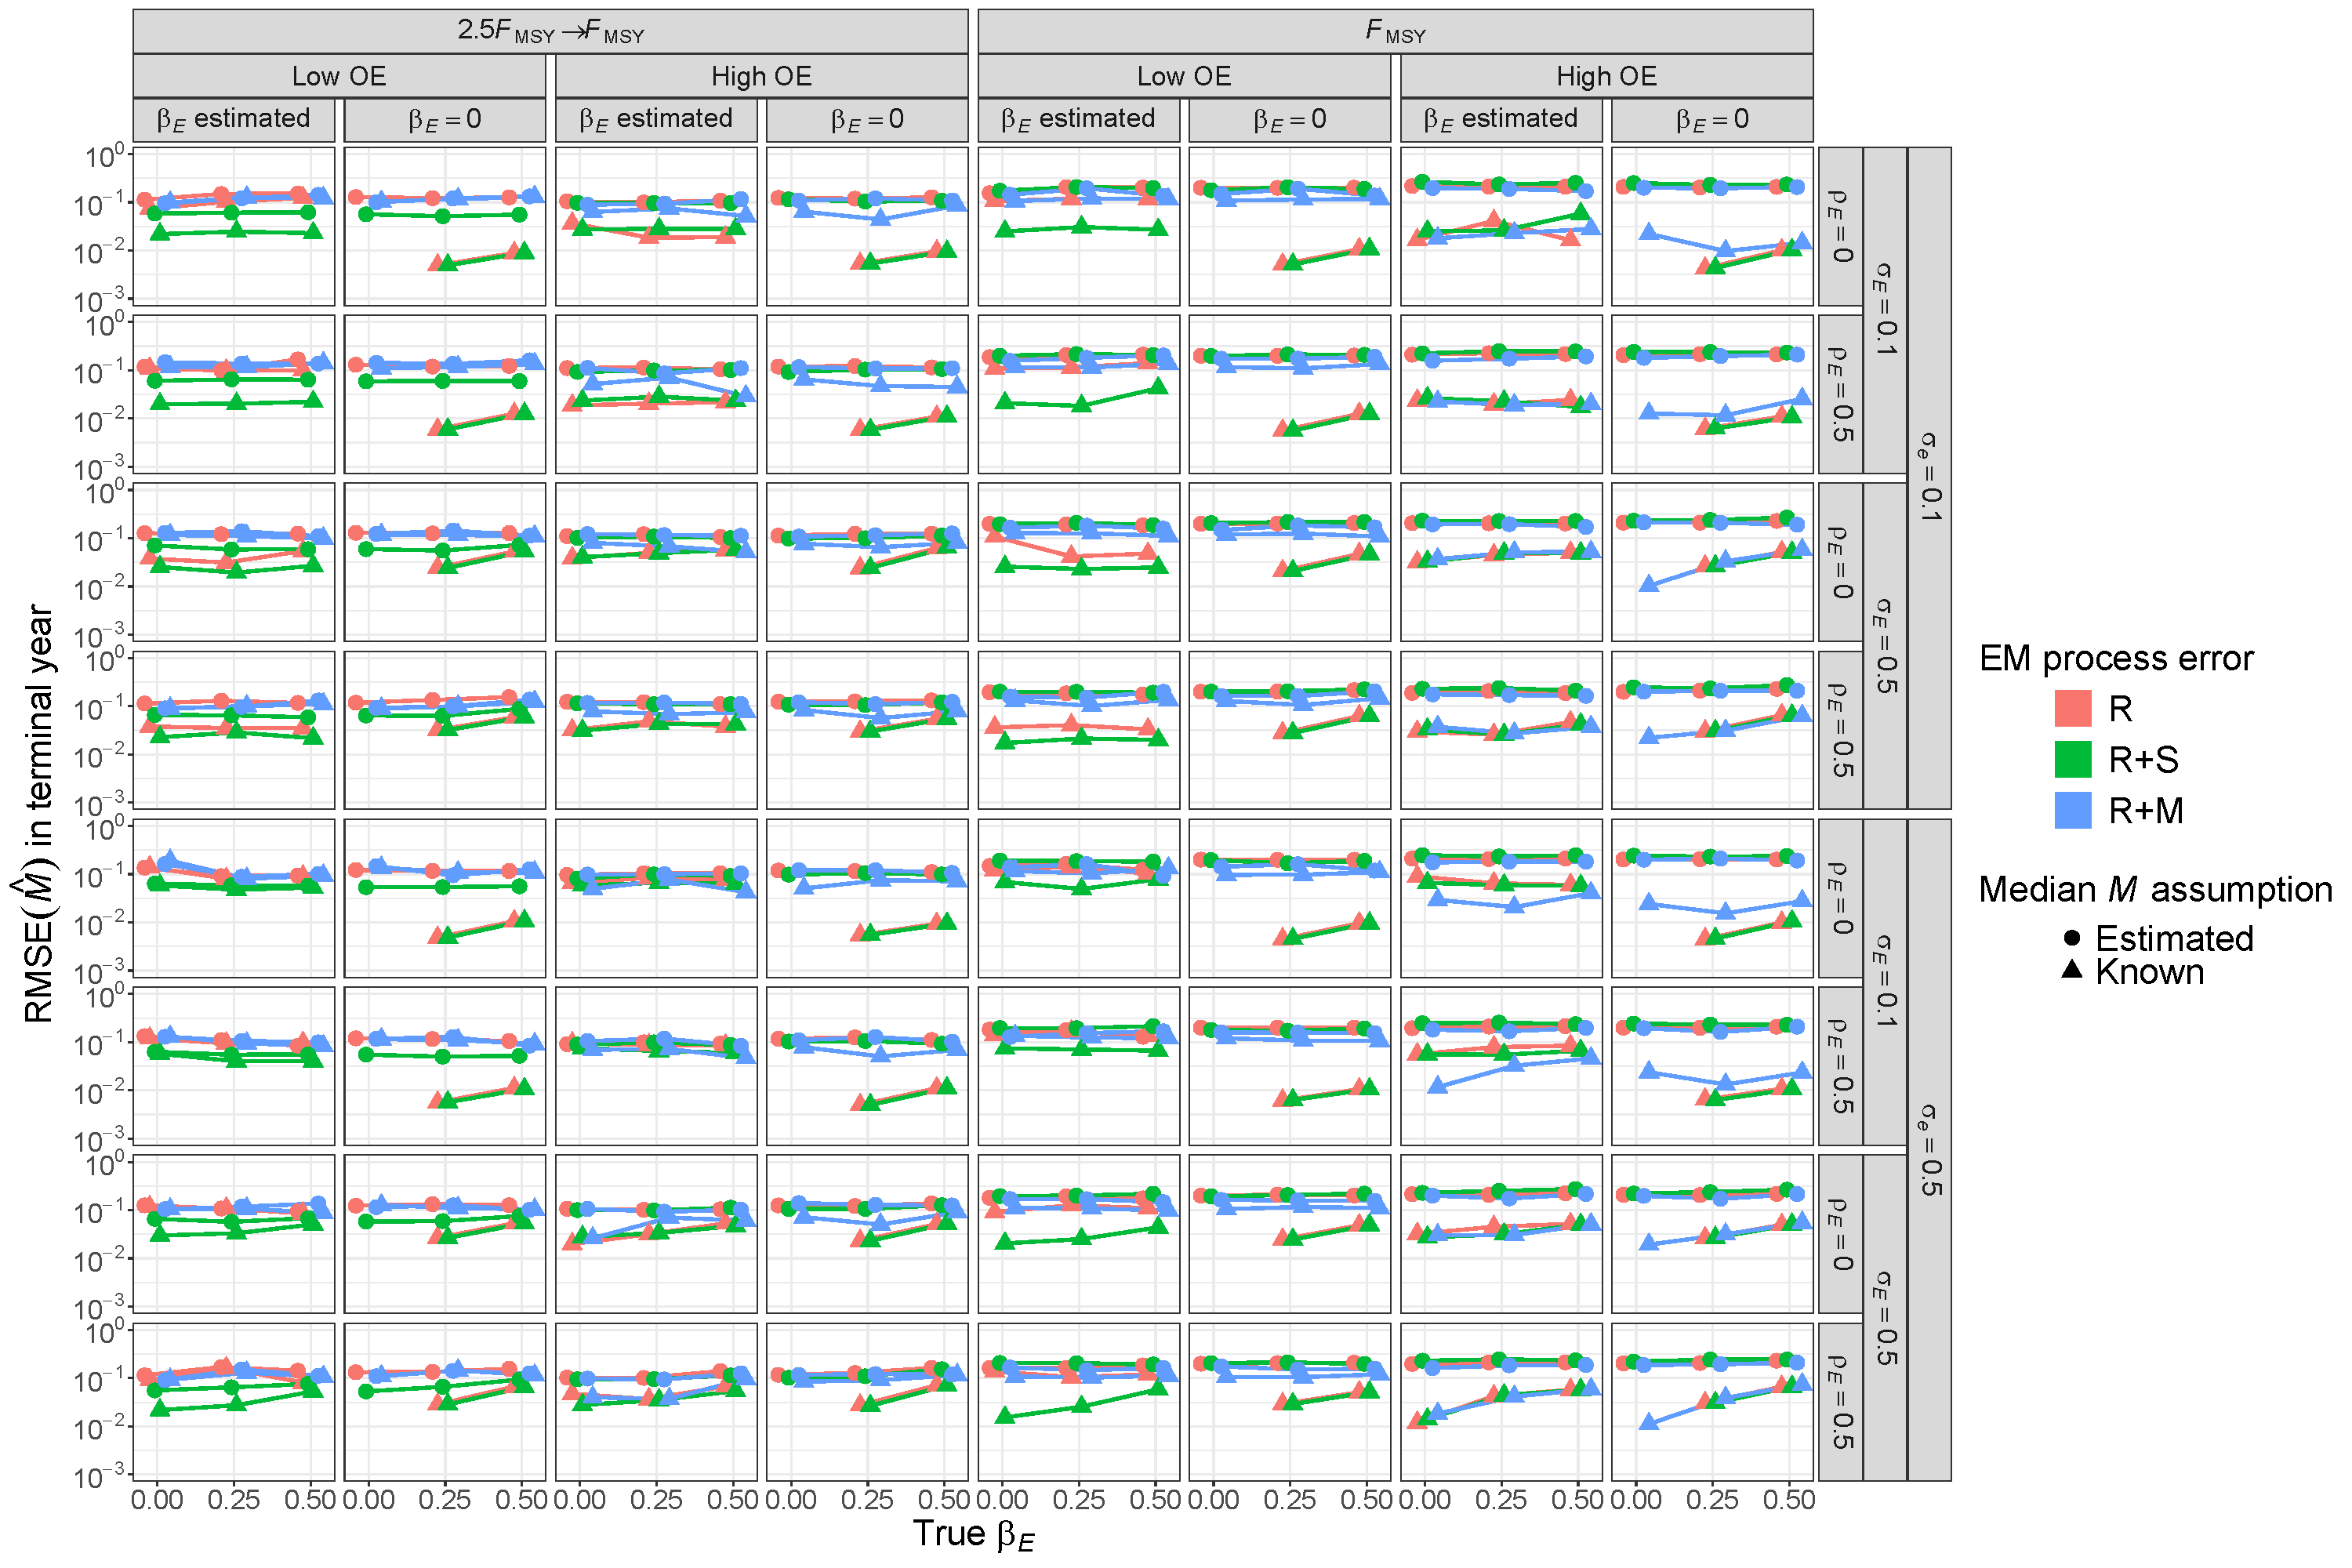
\includegraphics[height = \textheight]{terminal_year_M_rmse_RSom}
%DIFDELCMD < %%%
\DIFdelendFL \DIFaddbeginFL 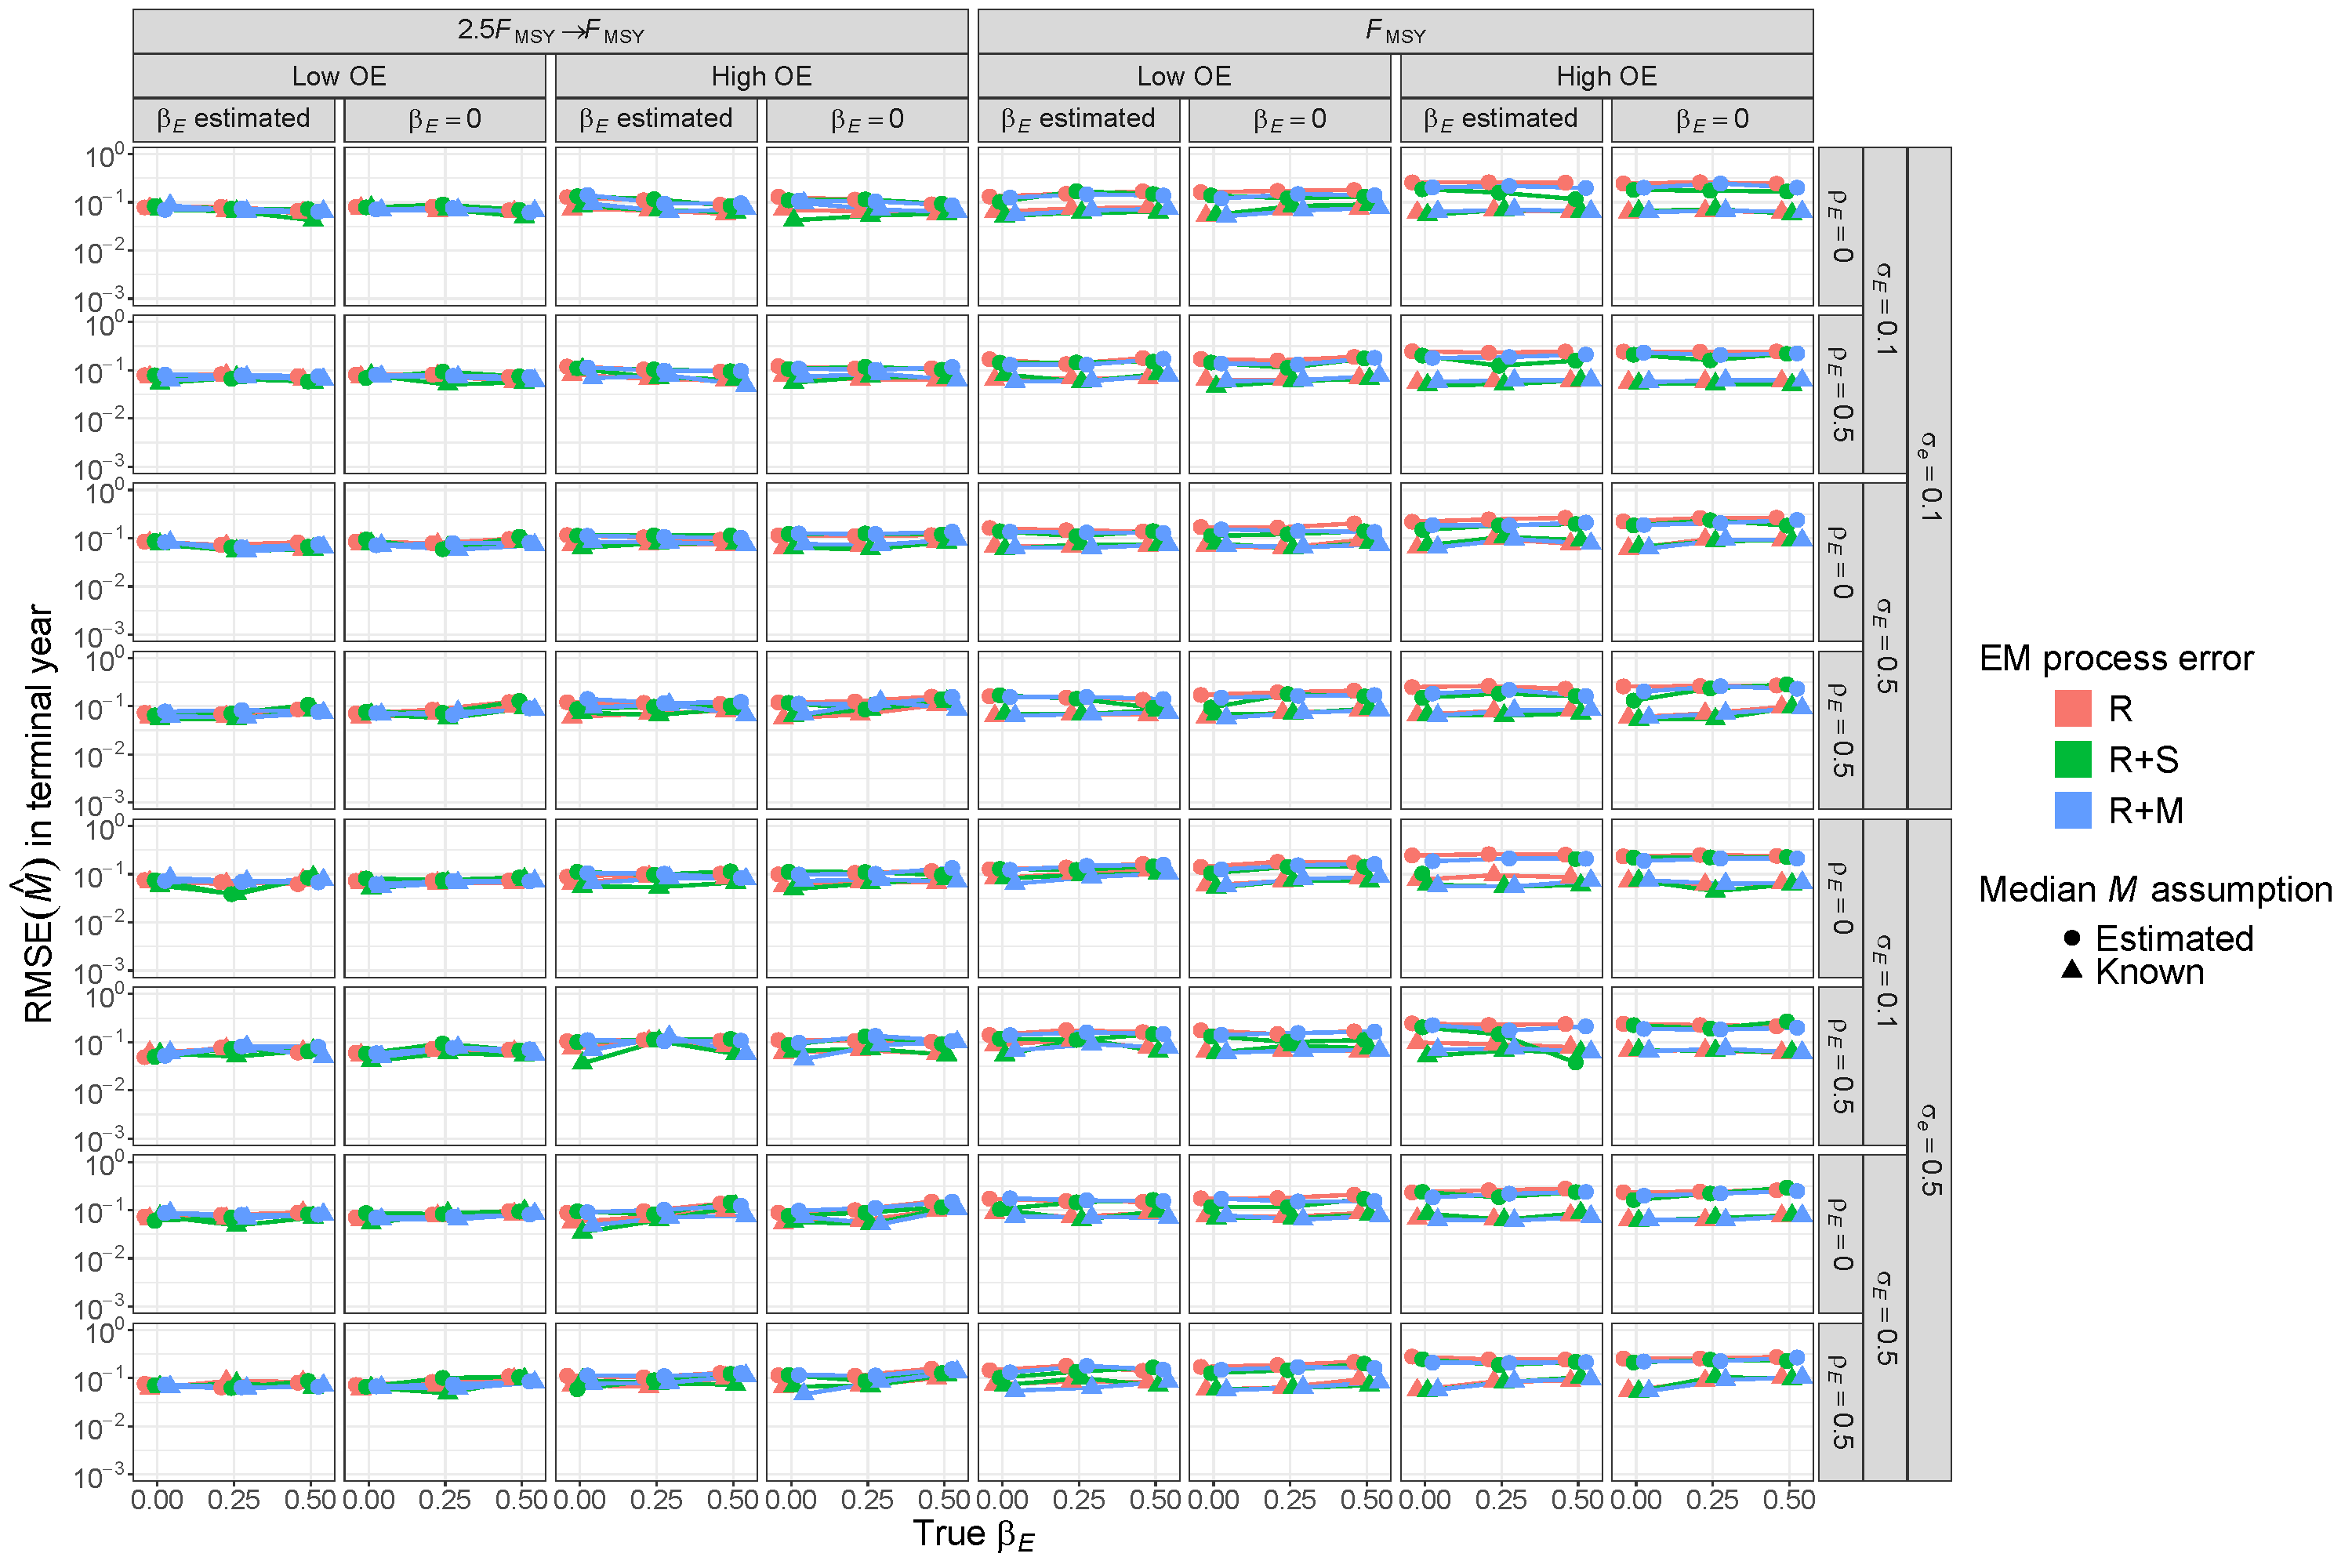
\includegraphics[height = \textheight]{terminal_year_M_rmse_RMom}
\DIFaddendFL \end{center}
\caption{For R+\DIFdelbeginFL \DIFdelFL{S }\DIFdelendFL \DIFaddbeginFL \DIFaddFL{M }\DIFaddendFL OMs, \DIFdelbeginFL \DIFdelFL{root mean square error (}\DIFdelendFL RMSE \DIFdelbeginFL \DIFdelFL{) }\DIFdelendFL of estimates of \DIFdelbeginFL \DIFdelFL{natural mortality rate in the }\DIFdelendFL terminal year \DIFaddbeginFL \DIFaddFL{$M$ }\DIFaddendFL for EMs with alternative process error assumptions, treatment of covariate effect ($\beta_E = 0$ or estimated), and treatment of median \DIFdelbeginFL \DIFdelFL{natural mortality }\DIFdelendFL \DIFaddbeginFL \DIFaddFL{$M$ }\DIFaddendFL parameter ($\beta_M$ estimated or known).}\DIFdelbeginFL %DIFDELCMD < \label{terminal_M_rmse_RSom}
%DIFDELCMD < %%%
\DIFdelendFL \DIFaddbeginFL \label{terminal_M_rmse_RMom}
\DIFaddendFL \end{figure}
\end{landscape}

\begin{landscape}
\begin{figure}
\begin{center}
\DIFdelbeginFL %DIFDELCMD < 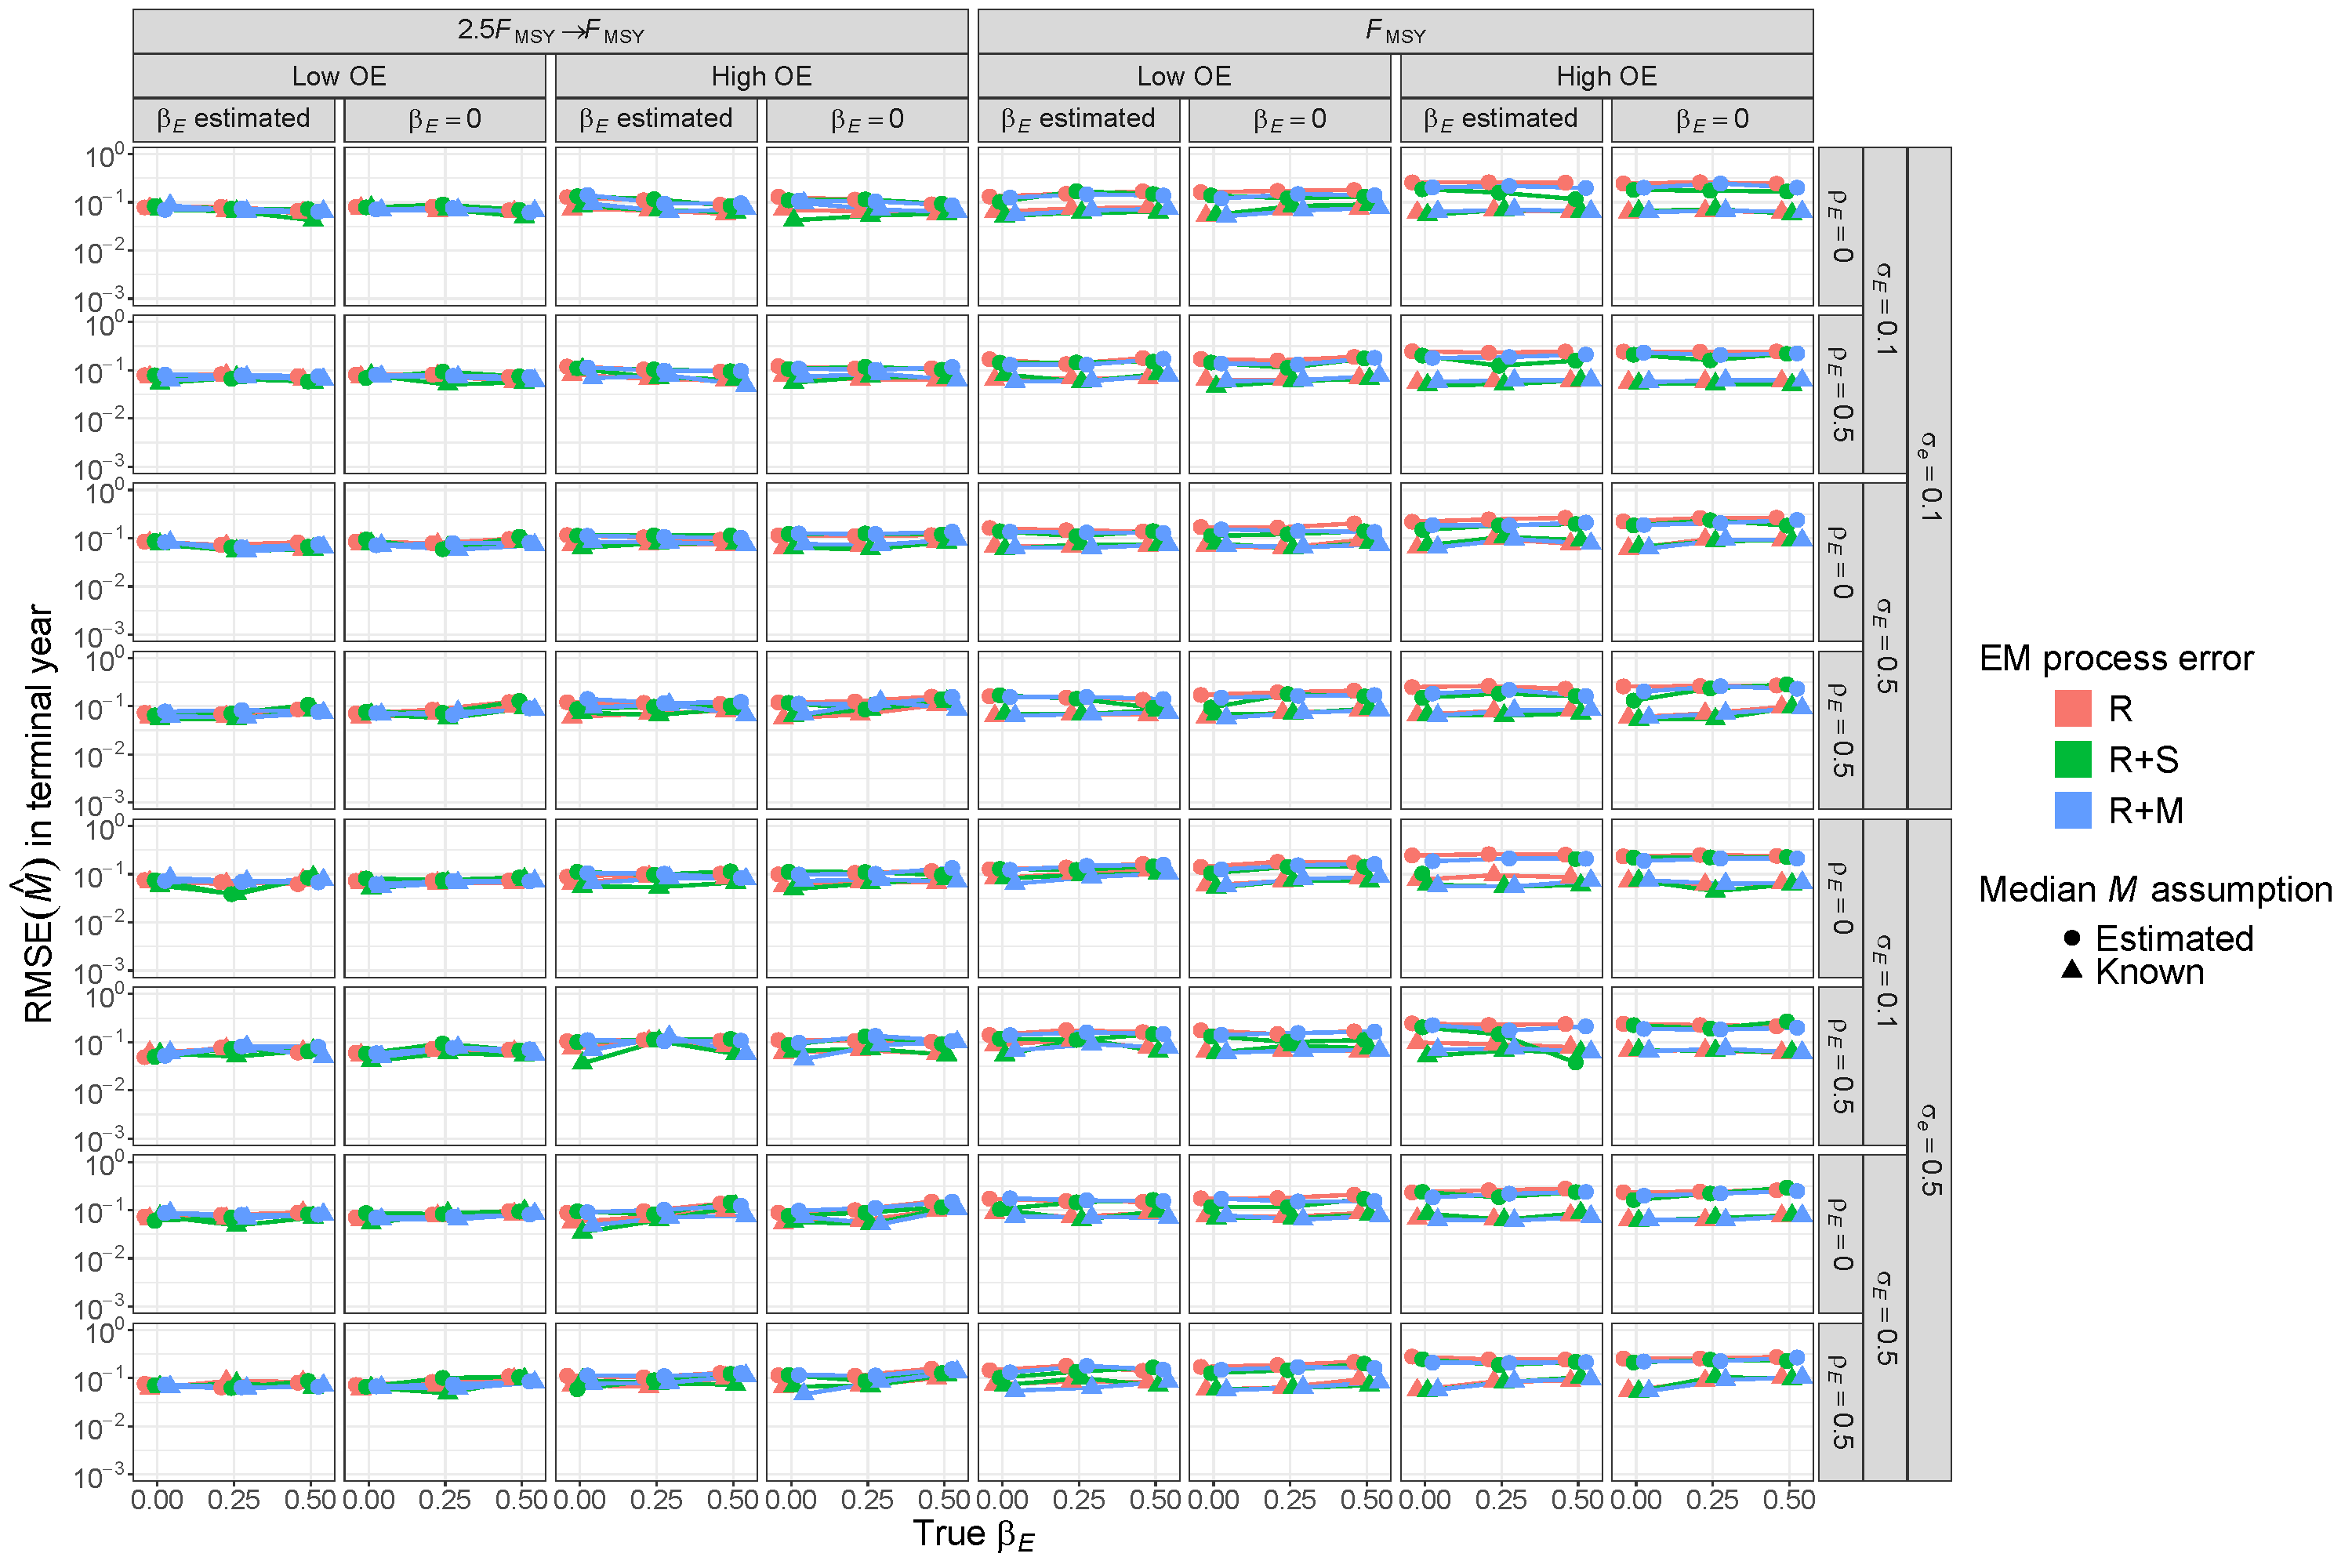
\includegraphics[height = \textheight]{terminal_year_M_rmse_RMom}
%DIFDELCMD < %%%
\DIFdelendFL \DIFaddbeginFL 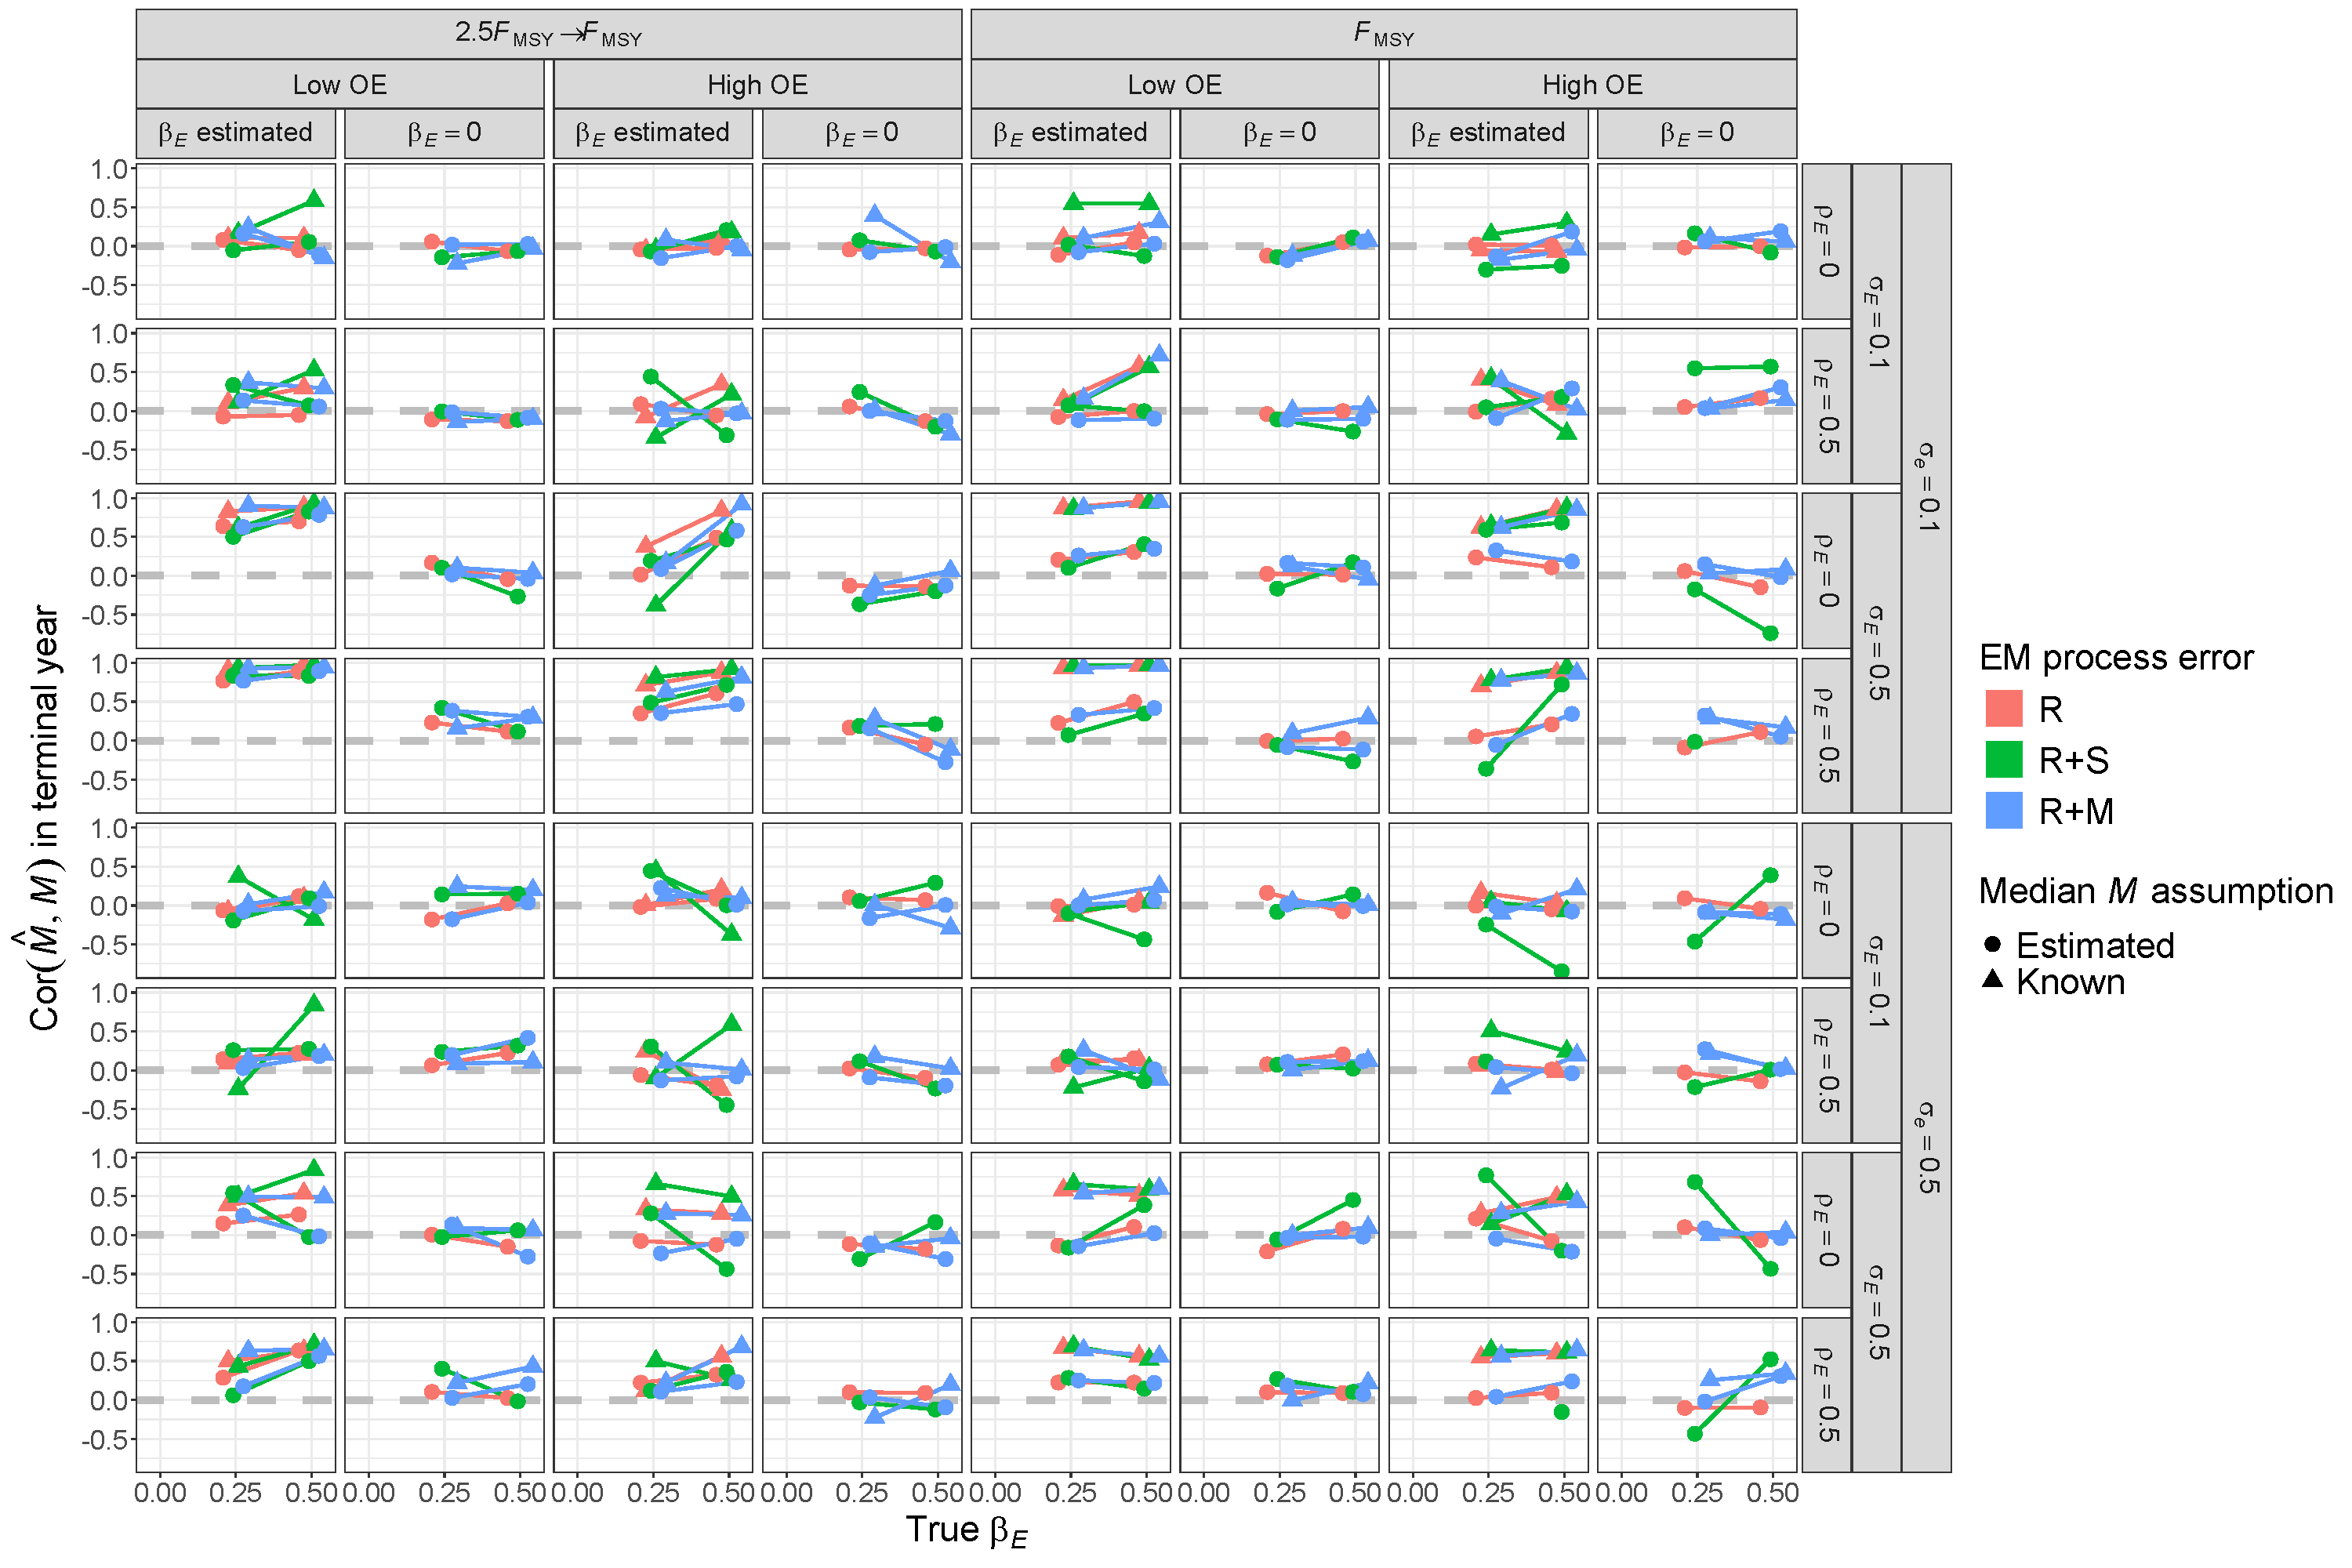
\includegraphics[height = \textheight]{terminal_year_M_corr_Rom}
\DIFaddendFL \end{center}
\caption{For R \DIFdelbeginFL \DIFdelFL{+M }\DIFdelendFL OMs, \DIFdelbeginFL \DIFdelFL{root mean square error (RMSE) }\DIFdelendFL \DIFaddbeginFL \DIFaddFL{correlation }\DIFaddendFL of estimates \DIFaddbeginFL \DIFaddFL{and true values }\DIFaddendFL of \DIFdelbeginFL \DIFdelFL{natural mortality rate in the }\DIFdelendFL terminal year \DIFaddbeginFL \DIFaddFL{$M$ }\DIFaddendFL for EMs with alternative process error assumptions, treatment of covariate effect ($\beta_E = 0$ or estimated), and treatment of median \DIFdelbeginFL \DIFdelFL{natural mortality }\DIFdelendFL \DIFaddbeginFL \DIFaddFL{$M$ }\DIFaddendFL parameter ($\beta_M$ estimated or known).}\DIFdelbeginFL %DIFDELCMD < \label{terminal_M_rmse_RMom}
%DIFDELCMD < %%%
\DIFdelendFL \DIFaddbeginFL \label{terminal_M_corr_Rom}
\DIFaddendFL \end{figure}
\end{landscape}

\DIFdelbegin %DIFDELCMD < \hypertarget{terminal-year-spawning-stock-biomass-bias}{%
%DIFDELCMD < \subsection*{Terminal year spawning stock biomass bias}\label{terminal-year-spawning-stock-biomass-bias}}
%DIFDELCMD < %%%
\DIFdelend \DIFaddbegin \begin{landscape}
\begin{figure}
\begin{center}
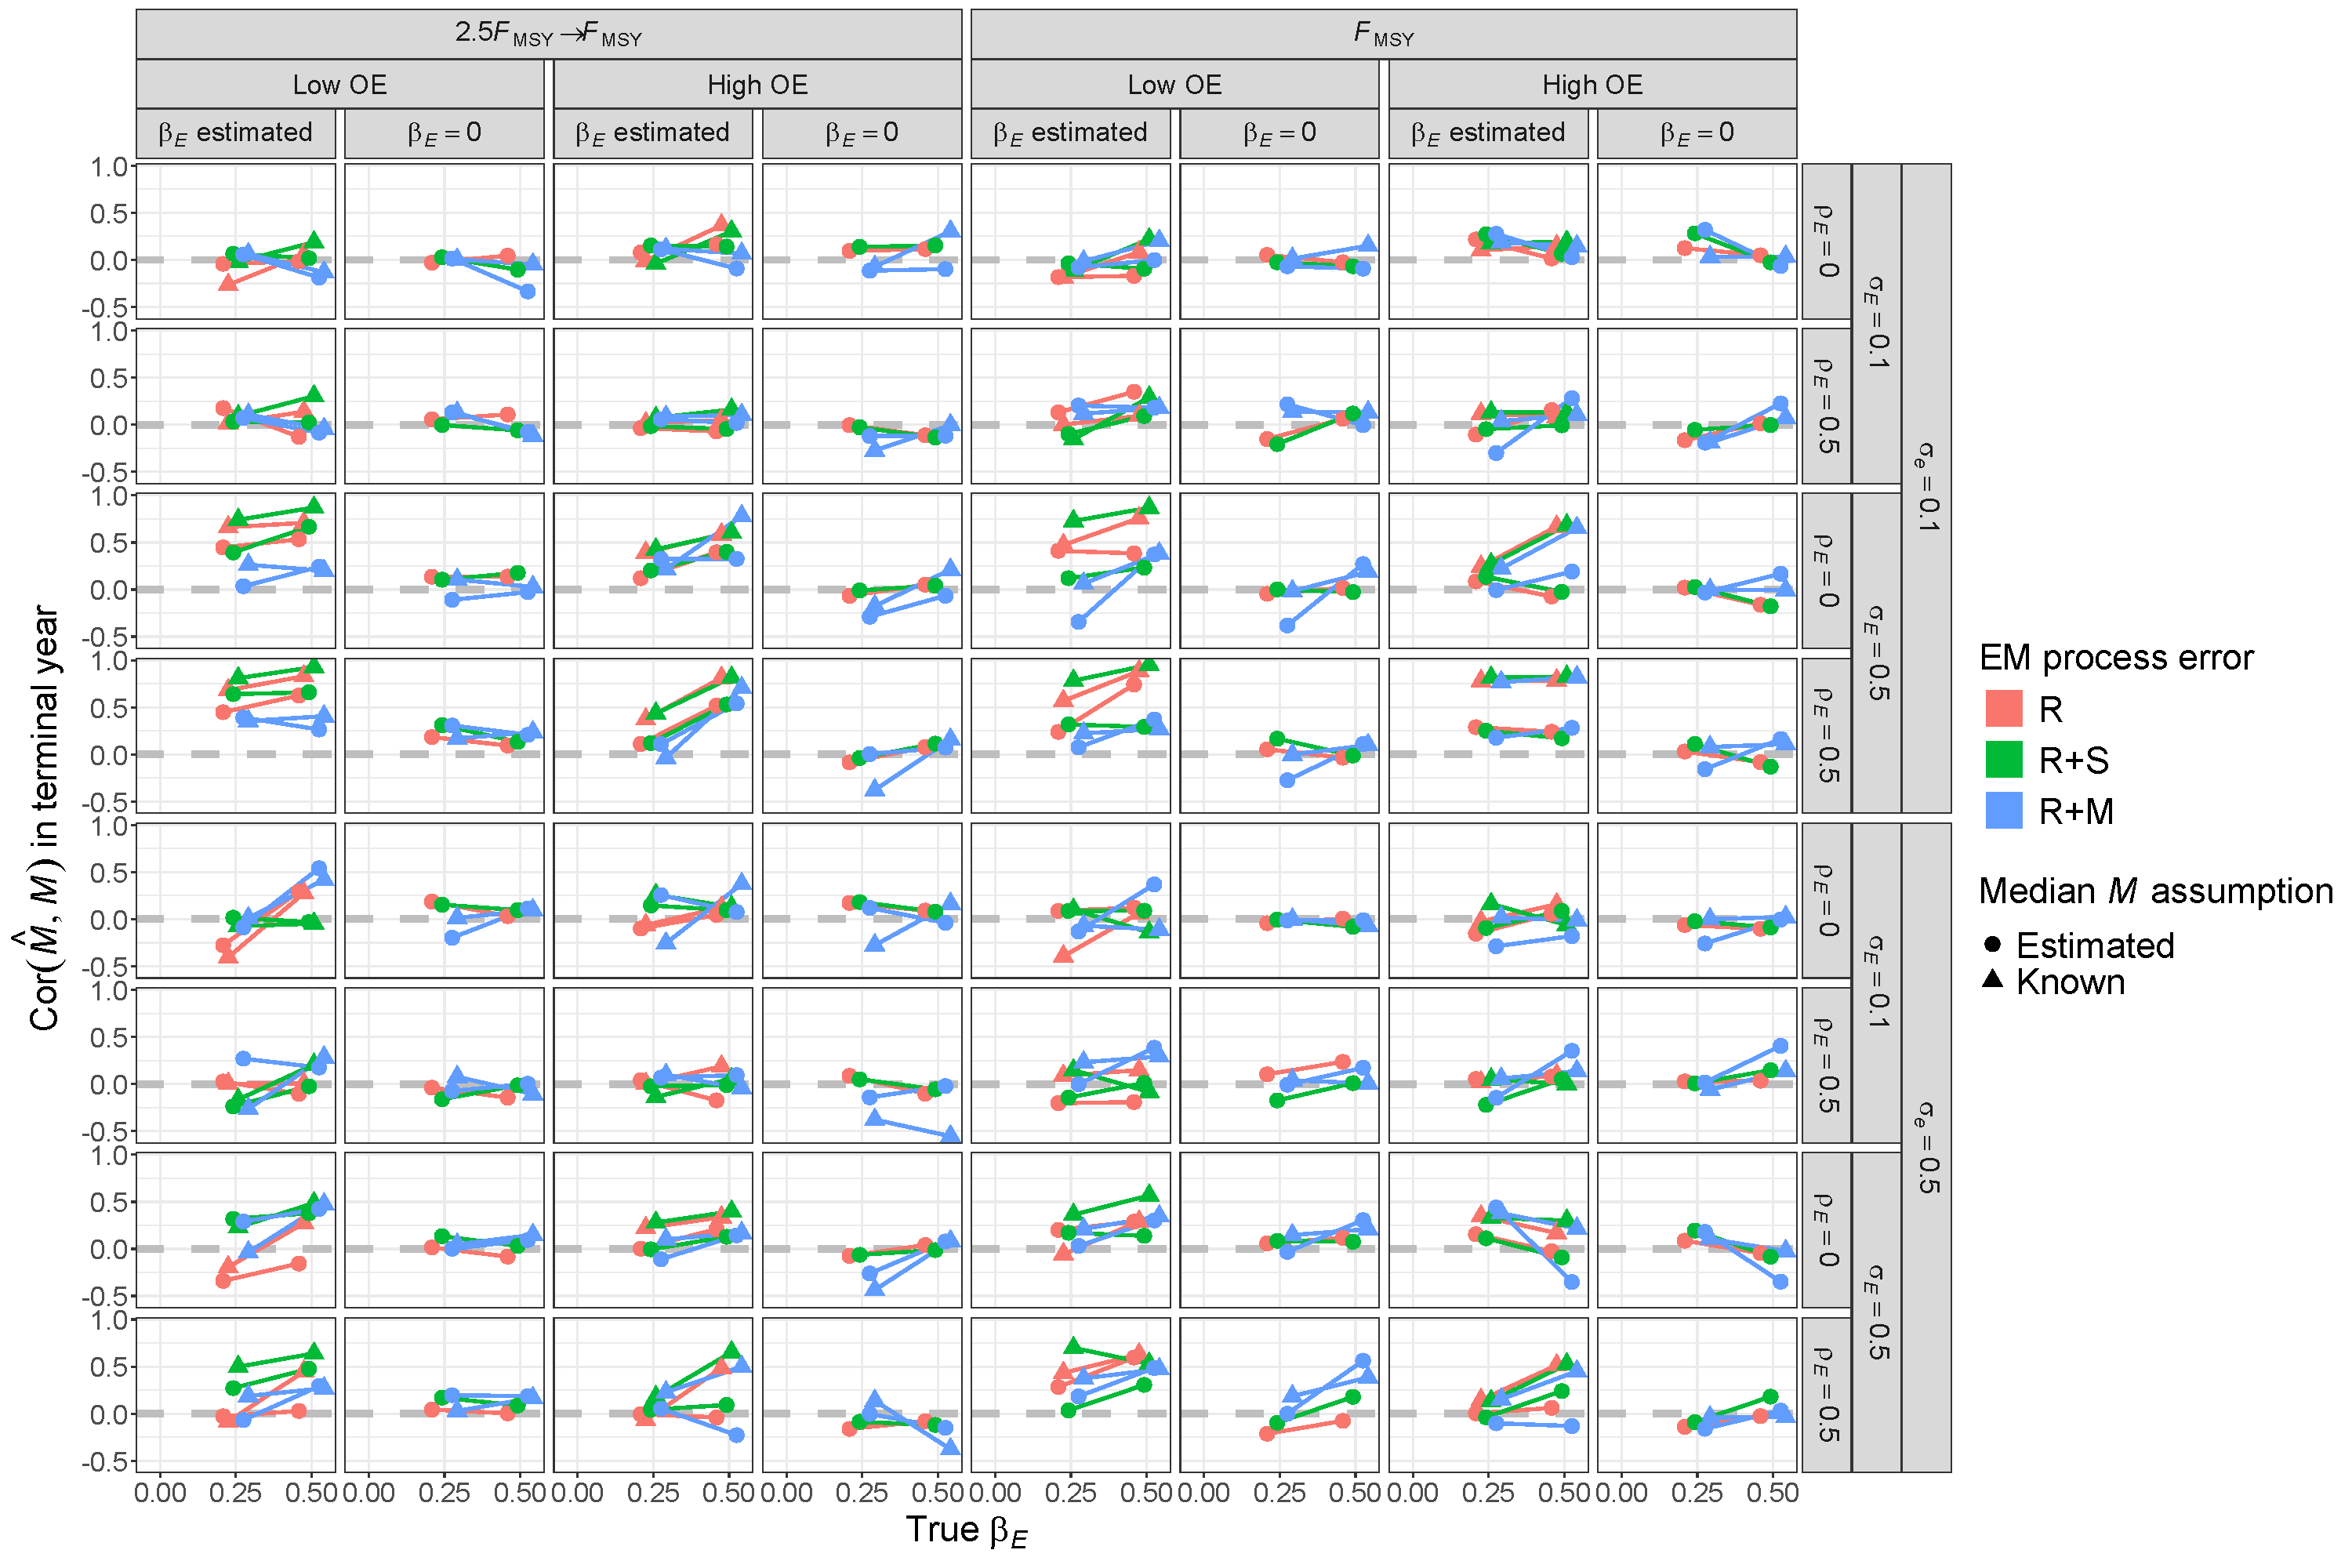
\includegraphics[height = \textheight]{terminal_year_M_corr_RSom}
\end{center}
\caption{\DIFaddFL{For R+S OMs, correlation of estimates and true values of terminal year $M$ for EMs with alternative process error assumptions, treatment of covariate effect ($\beta_E = 0$ or estimated), and treatment of median $M$ parameter ($\beta_M$ estimated or known).}}\label{terminal_M_corr_RSom}
\end{figure}
\end{landscape}

\begin{landscape}
\begin{figure}
\begin{center}
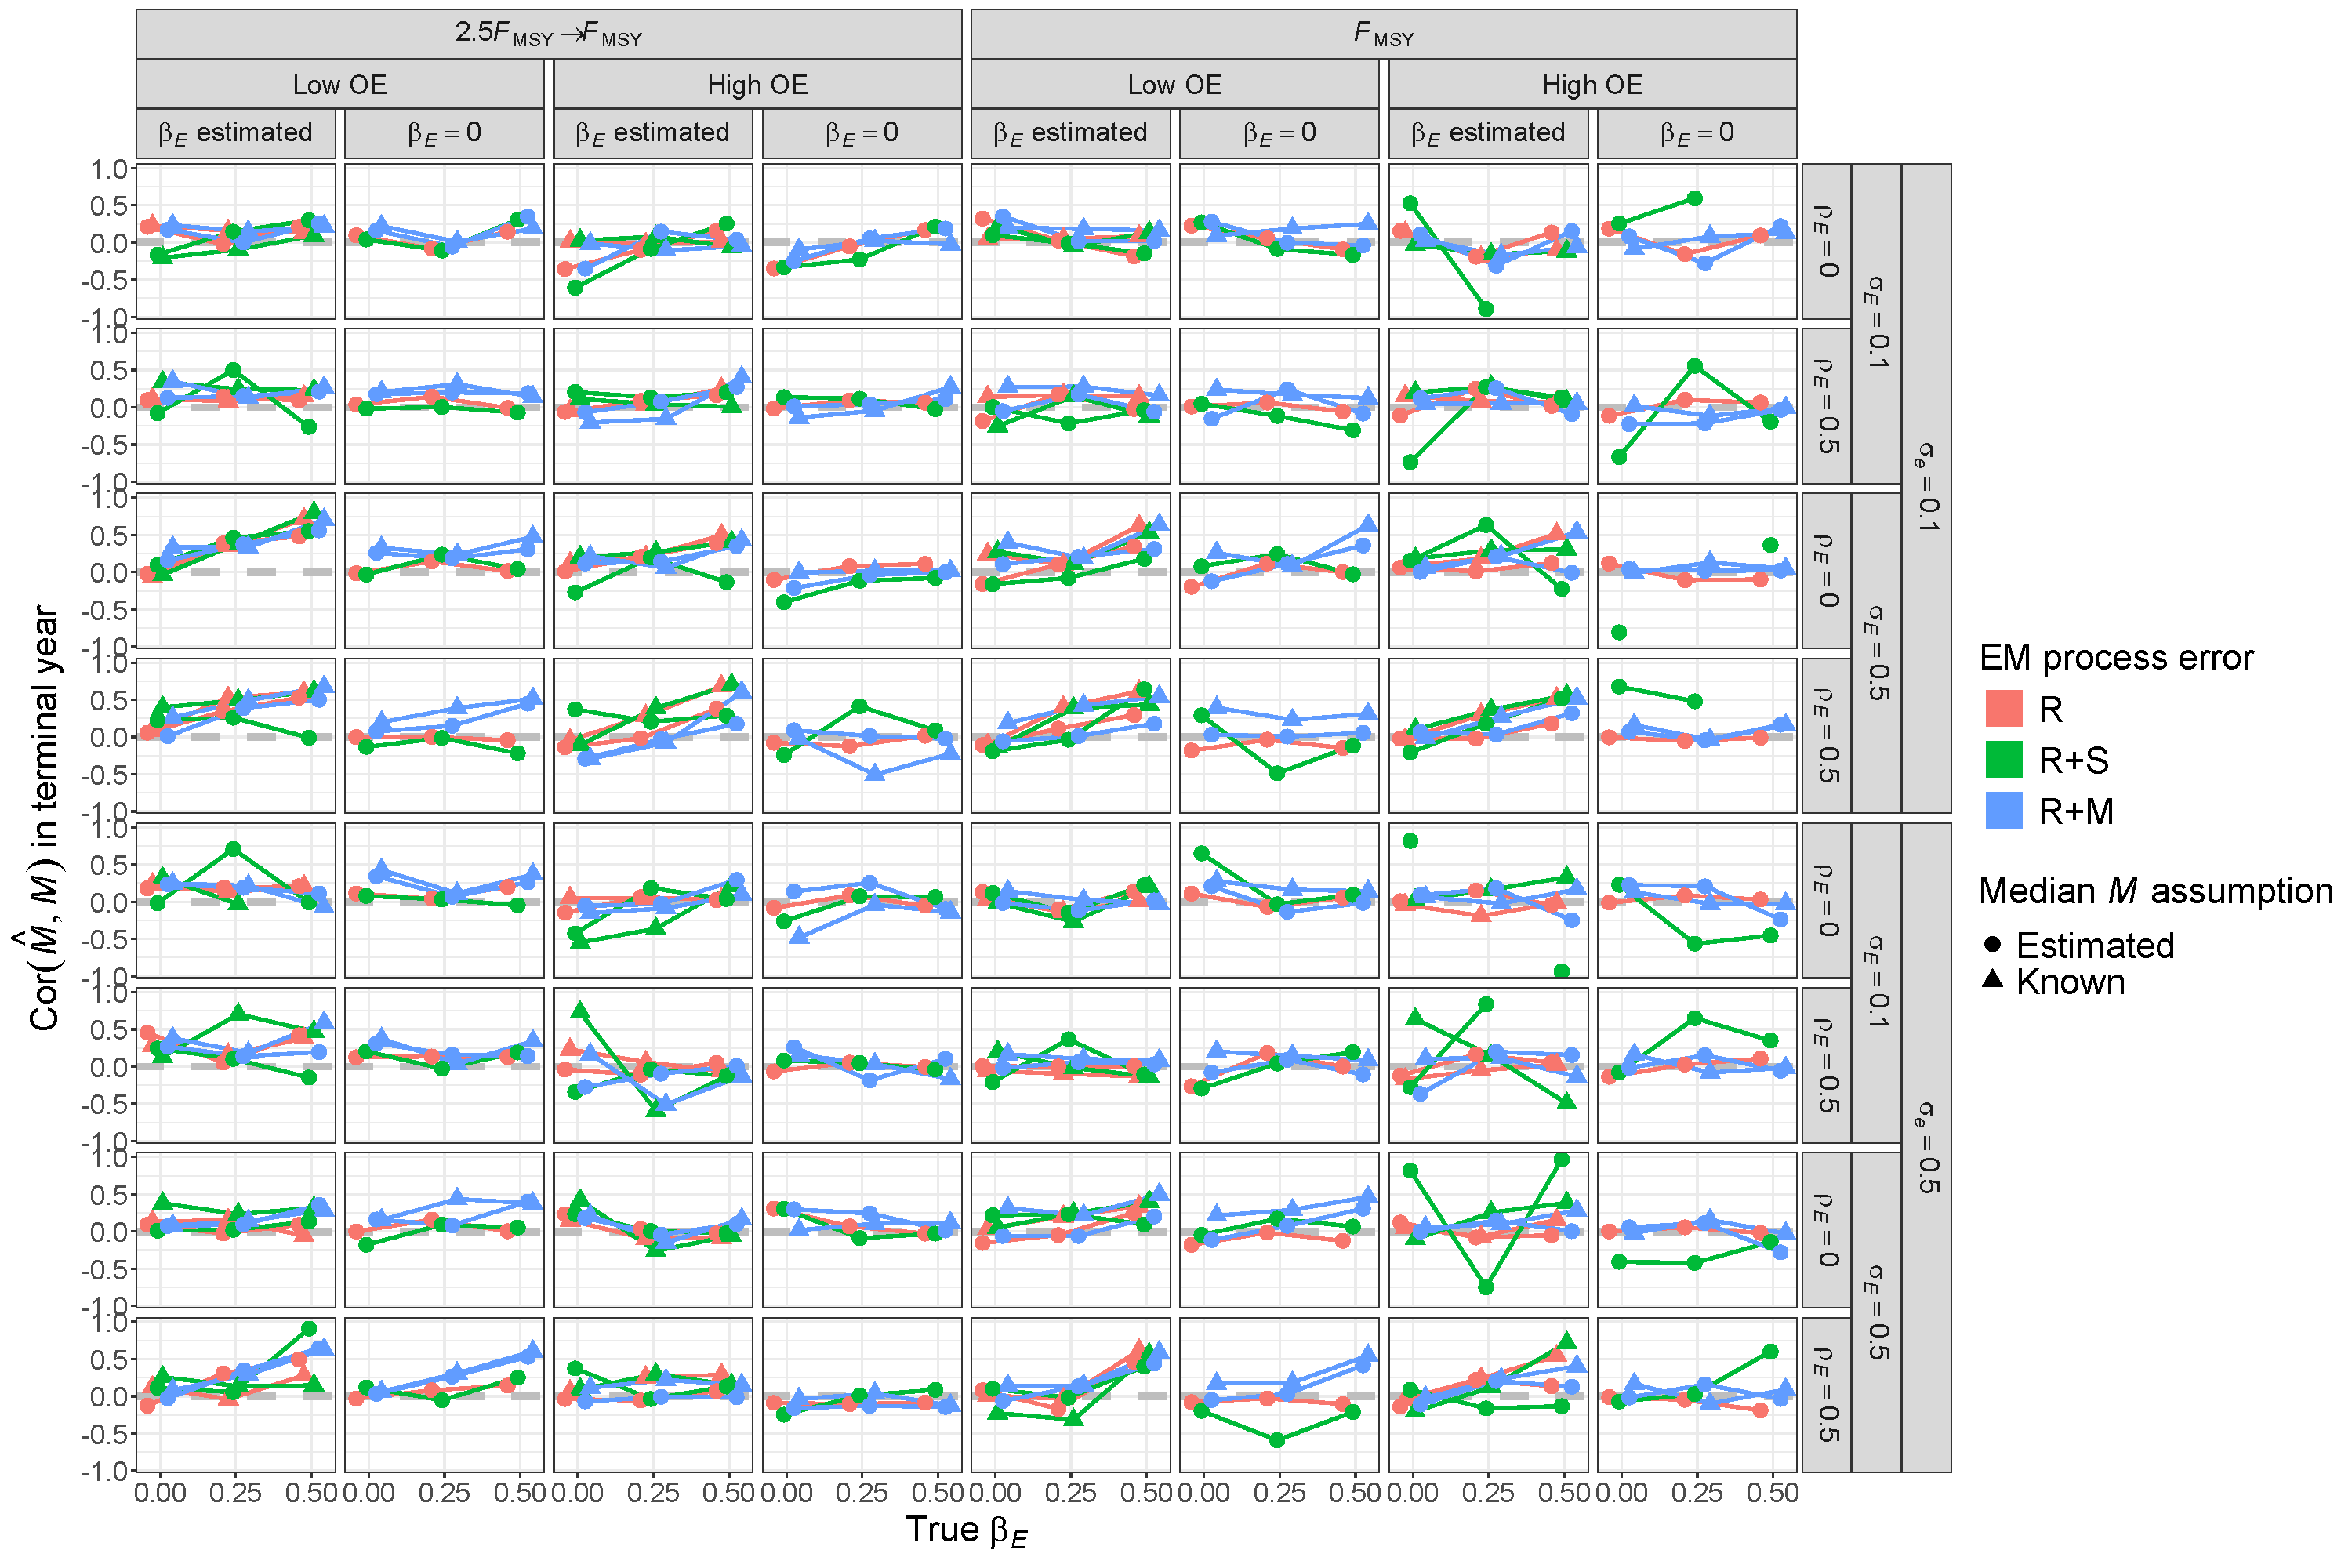
\includegraphics[height = \textheight]{terminal_year_M_corr_RMom}
\end{center}
\caption{\DIFaddFL{For R+M OMs, correlation of estimates and true vales of terminal year $M$ for EMs with alternative process error assumptions, treatment of covariate effect ($\beta_E = 0$ or estimated), and treatment of median $M$ parameter ($\beta_M$ estimated or known).}}\label{terminal_M_corr_RMom}
\end{figure}
\end{landscape}

\subsection*{\DIFadd{Terminal year spawning stock biomass bias}}\label{terminal-year-spawning-stock-biomass-bias}
\DIFaddend \addcontentsline{toc}{subsection}{Terminal year spawning stock biomass bias}

\begin{landscape}
\begin{figure}
\begin{center}
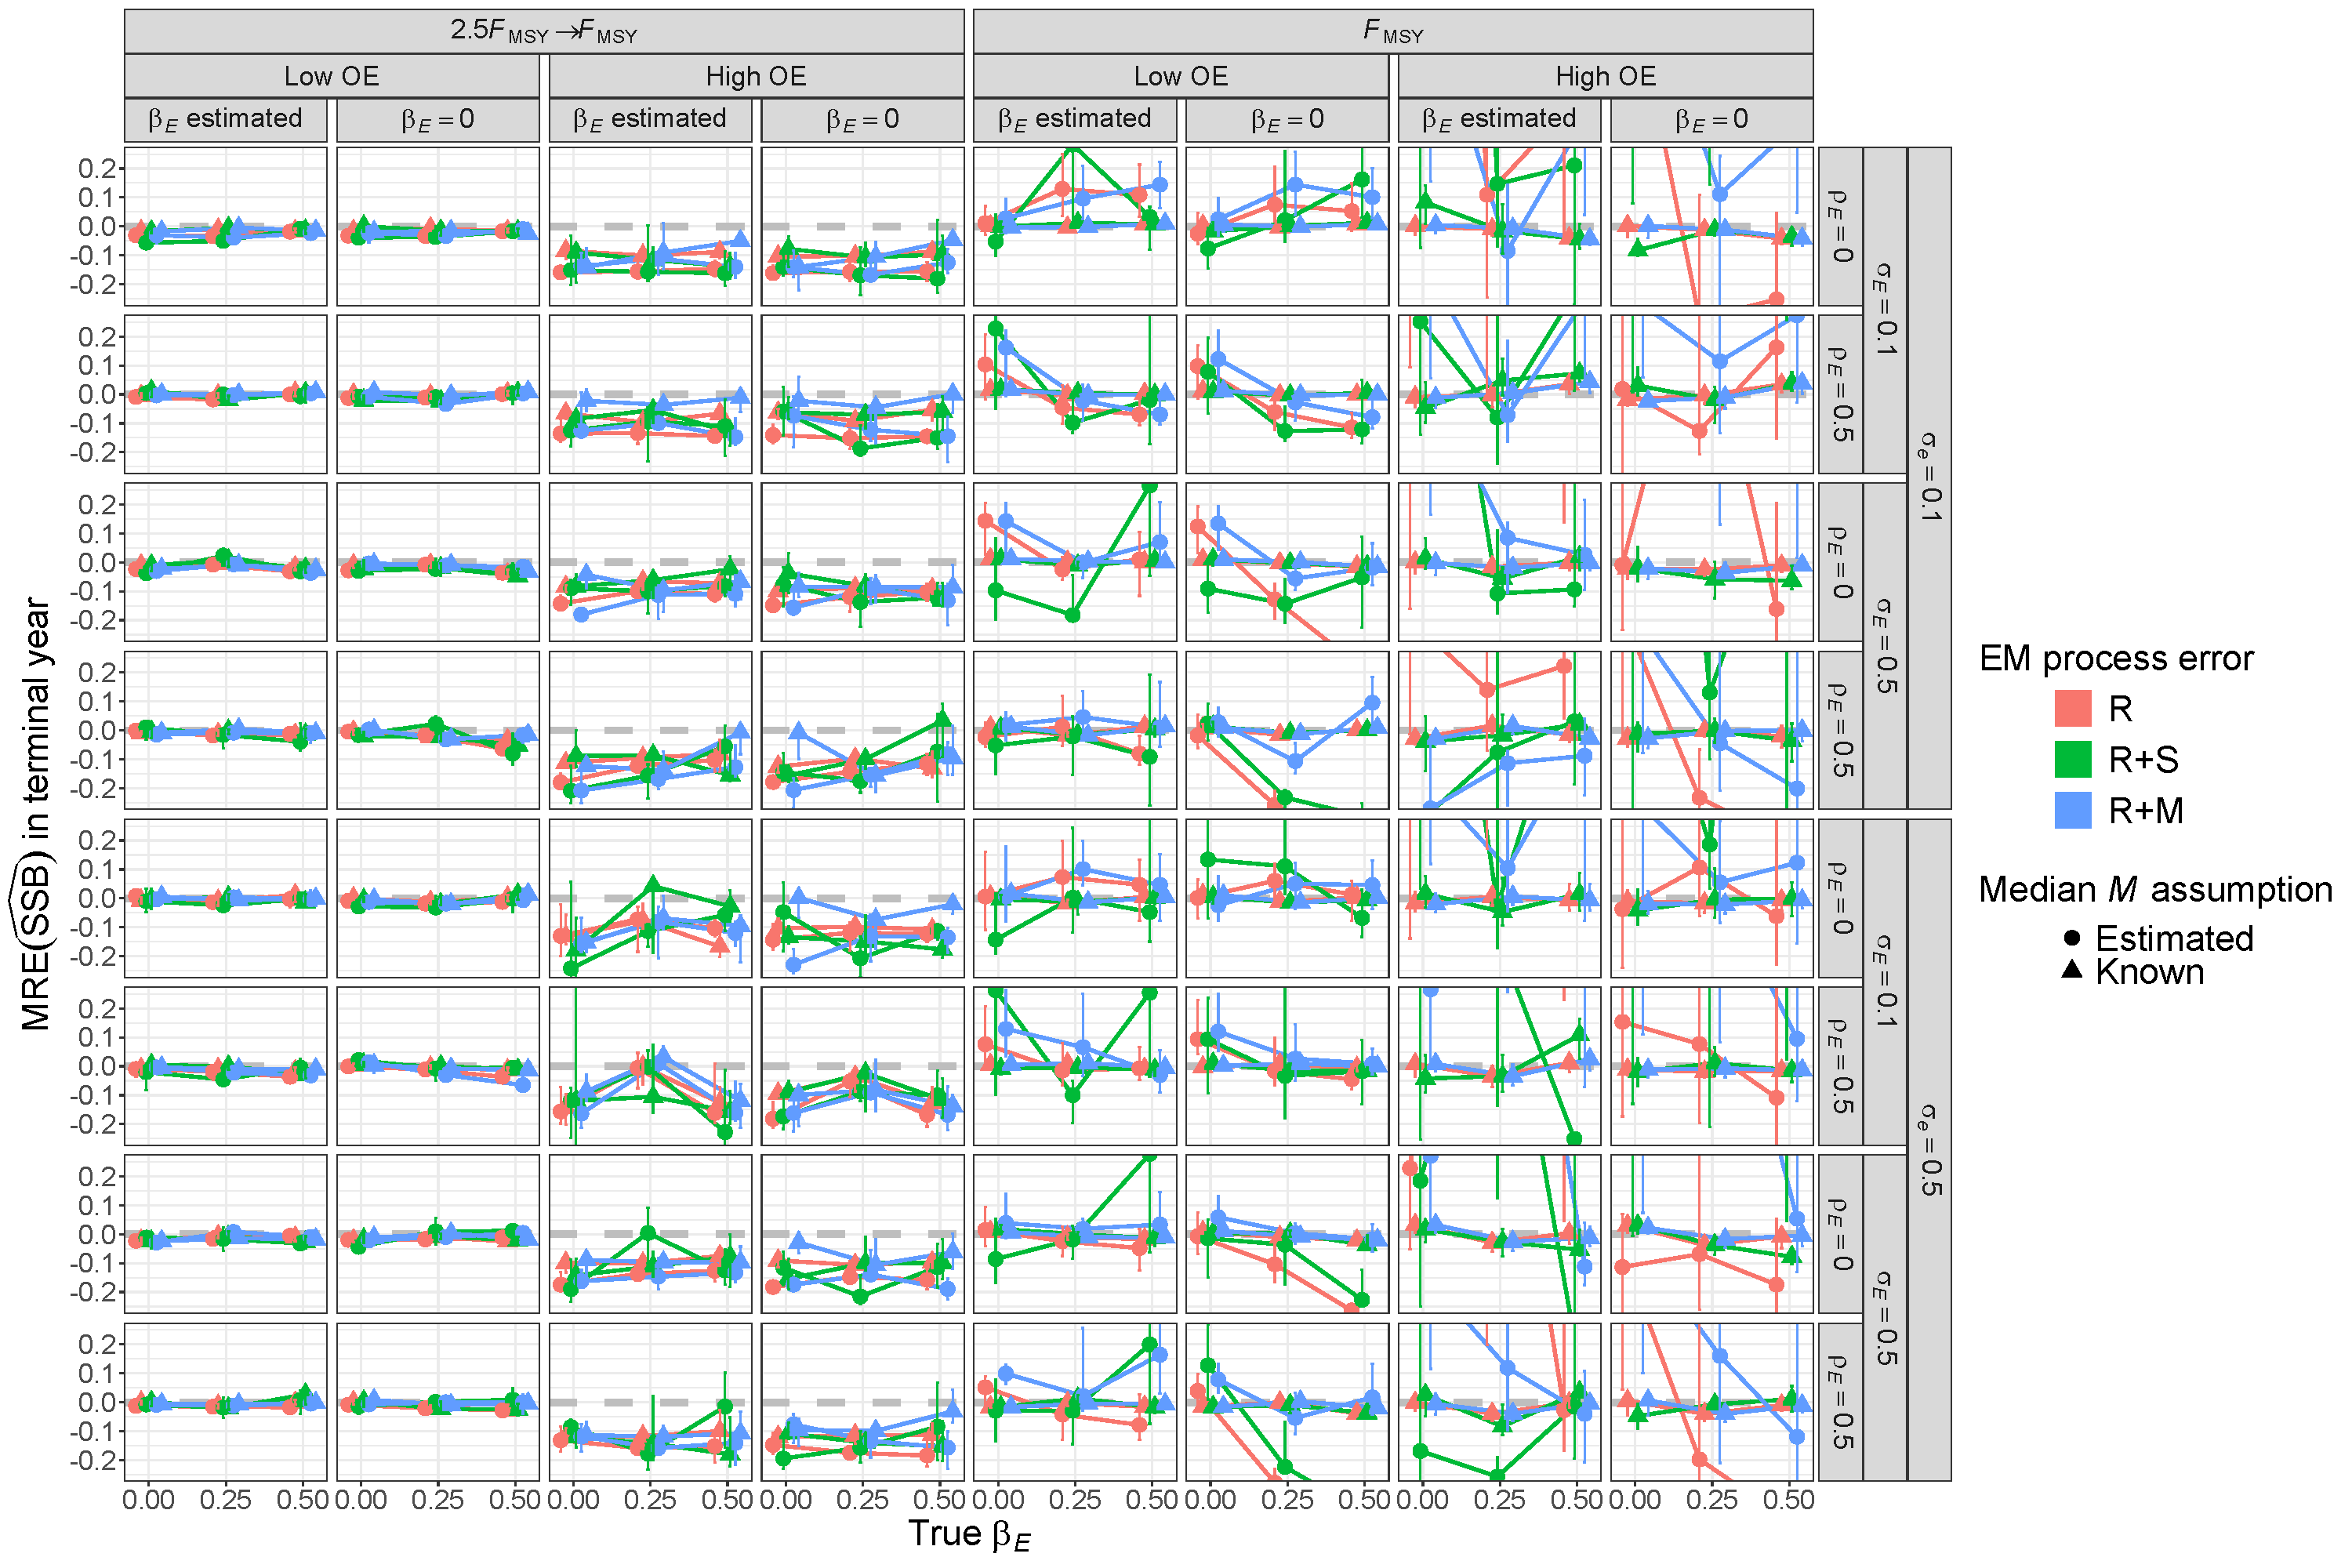
\includegraphics[height = \textheight]{terminal_year_ssb_bias_Rom}
\end{center}
\caption{For R OMs, median relative error (MRE) of estimates of \DIFdelbeginFL \DIFdelFL{spawning stock biomass (}\DIFdelendFL SSB \DIFdelbeginFL \DIFdelFL{) }\DIFdelendFL in the terminal year for EMs with alternative process error assumptions, treatment of covariate effect ($\beta_E = 0$ or estimated), and treatment of median \DIFdelbeginFL \DIFdelFL{natural mortality }\DIFdelendFL \DIFaddbeginFL \DIFaddFL{$M$ }\DIFaddendFL parameter ($\beta_M$ estimated or known).}\label{terminal_ssb_bias_Rom}
\end{figure}
\end{landscape}

\begin{landscape}
\begin{figure}
\begin{center}
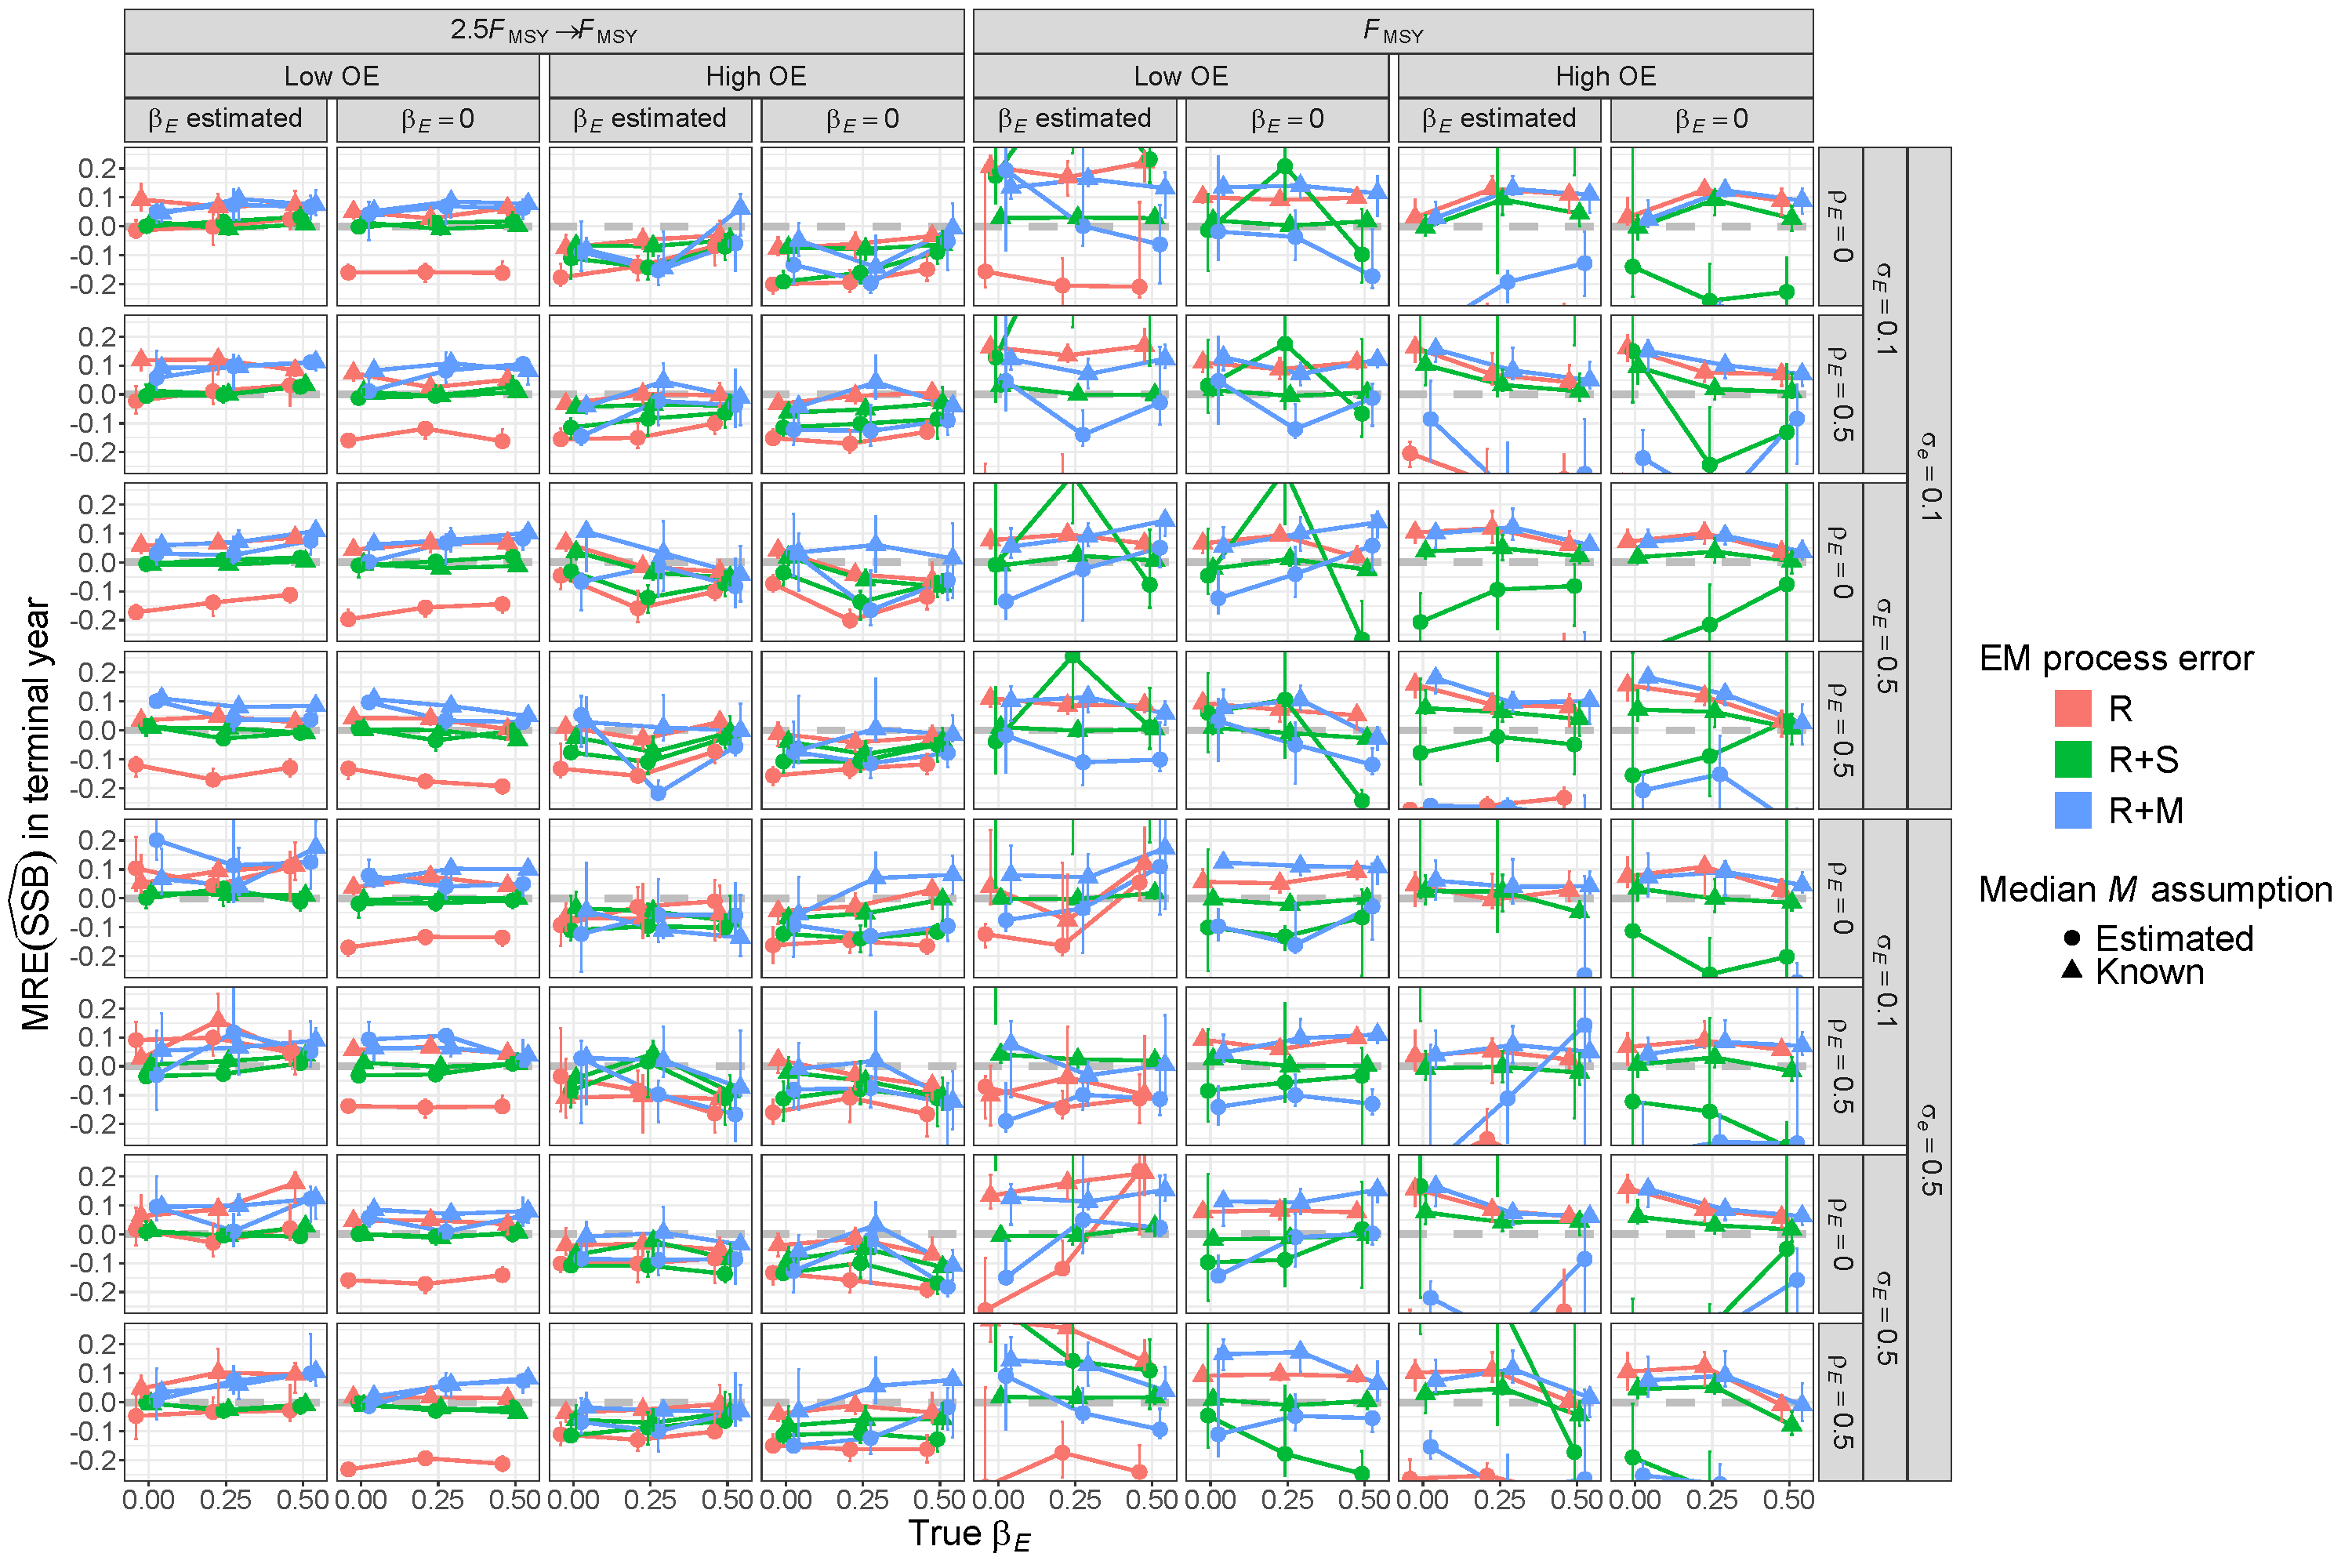
\includegraphics[height = \textheight]{terminal_year_ssb_bias_RSom}
\end{center}
\caption{For R+S OMs, median relative error (MRE) of \DIFdelbeginFL \DIFdelFL{estimates of spawning stock biomass (}\DIFdelendFL SSB \DIFdelbeginFL \DIFdelFL{) }\DIFdelendFL in the terminal year for EMs with alternative process error assumptions, treatment of covariate effect ($\beta_E = 0$ or estimated), and treatment of median \DIFdelbeginFL \DIFdelFL{natural mortality }\DIFdelendFL \DIFaddbeginFL \DIFaddFL{$M$ }\DIFaddendFL parameter ($\beta_M$ estimated or known).}\label{terminal_ssb_bias_RSom}
\end{figure}
\end{landscape}

\begin{landscape}
\begin{figure}
\begin{center}
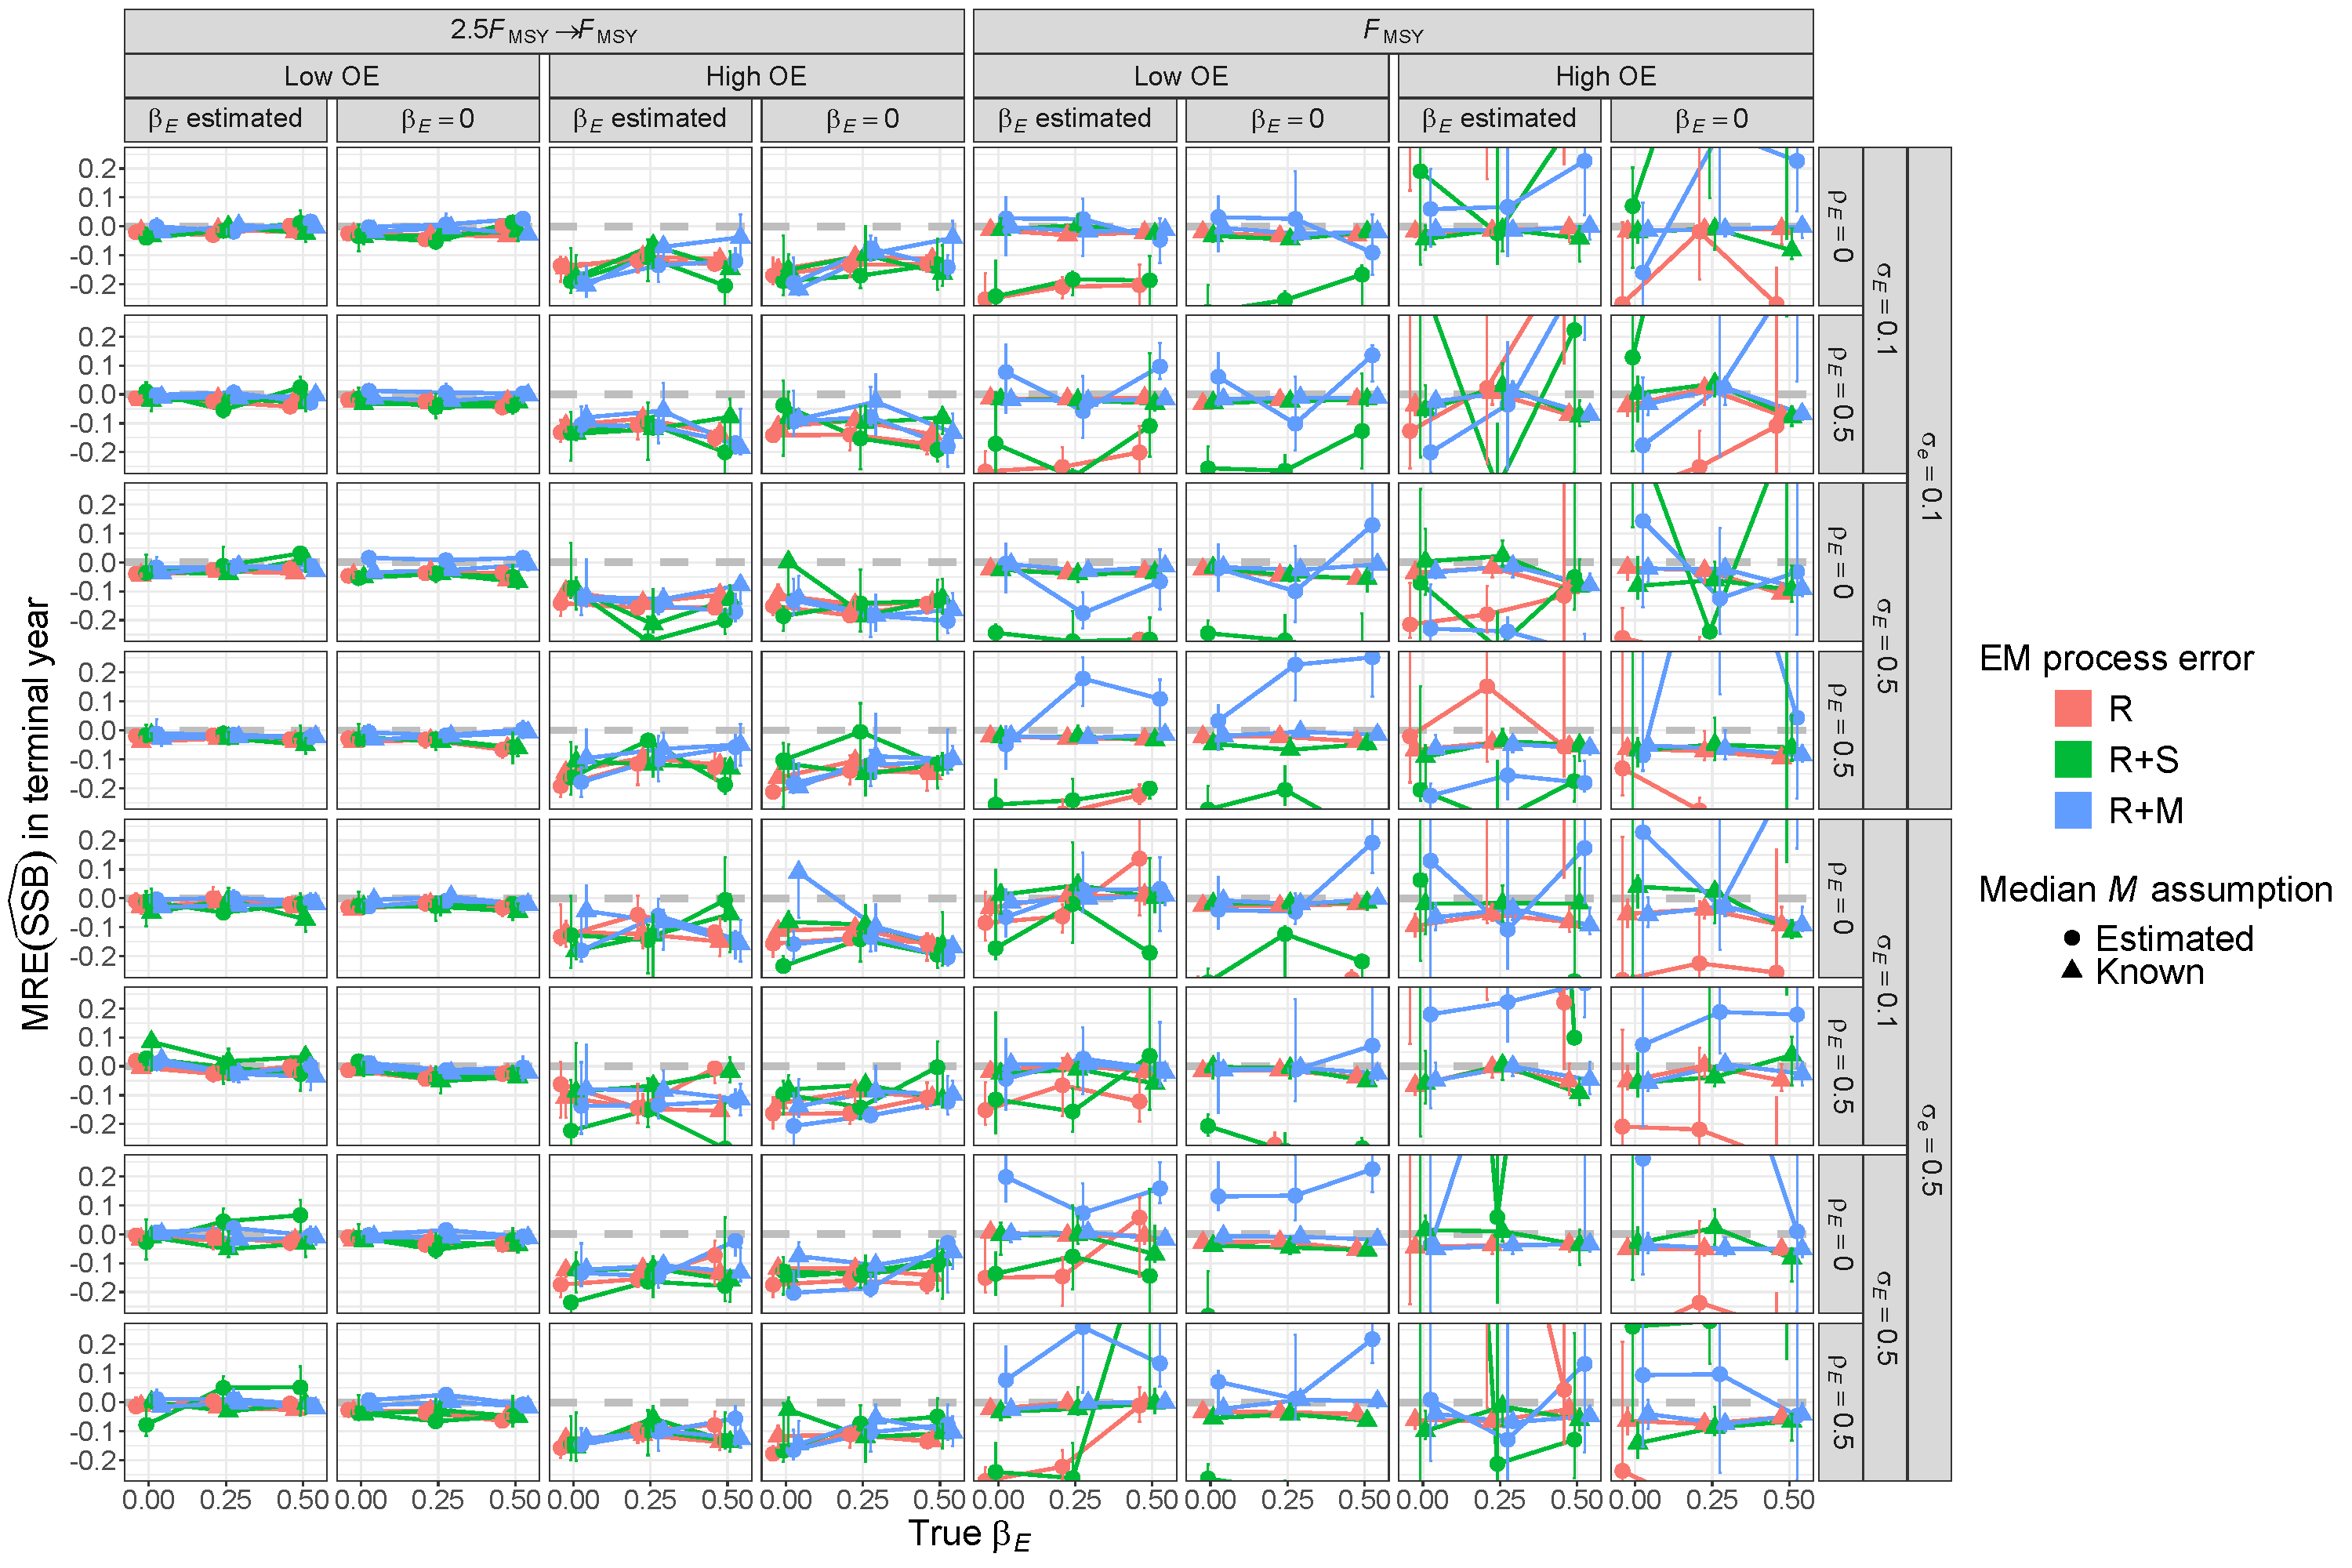
\includegraphics[height = \textheight]{terminal_year_ssb_bias_RMom}
\end{center}
\caption{For R+M OMs, median relative error (MRE) of estimates of \DIFdelbeginFL \DIFdelFL{spawning stock biomass (}\DIFdelendFL SSB \DIFdelbeginFL \DIFdelFL{) }\DIFdelendFL in the terminal year for EMs with alternative process error assumptions, treatment of covariate effect ($\beta_E = 0$ or estimated), and treatment of median \DIFdelbeginFL \DIFdelFL{natural mortality }\DIFdelendFL \DIFaddbeginFL \DIFaddFL{$M$ }\DIFaddendFL parameter ($\beta_M$ estimated or known).}\label{terminal_ssb_bias_RMom}
\end{figure}
\end{landscape}

\DIFdelbegin %DIFDELCMD < \hypertarget{terminal-year-spawning-stock-biomass-rmse}{%
%DIFDELCMD < \subsection*{Terminal year spawning stock biomass RMSE}\label{terminal-year-spawning-stock-biomass-rmse}}
%DIFDELCMD < %%%
\DIFdelend \DIFaddbegin \subsection*{\DIFadd{Terminal year spawning stock biomass accuracy}}\label{terminal-year-spawning-stock-biomass-accuracy}
\DIFaddend \addcontentsline{toc}{subsection}{Terminal year spawning stock biomass \DIFdelbegin \DIFdel{RMSE}\DIFdelend \DIFaddbegin \DIFadd{accuracy}\DIFaddend }

\begin{landscape}
\begin{figure}
\begin{center}
\DIFdelbeginFL %DIFDELCMD < 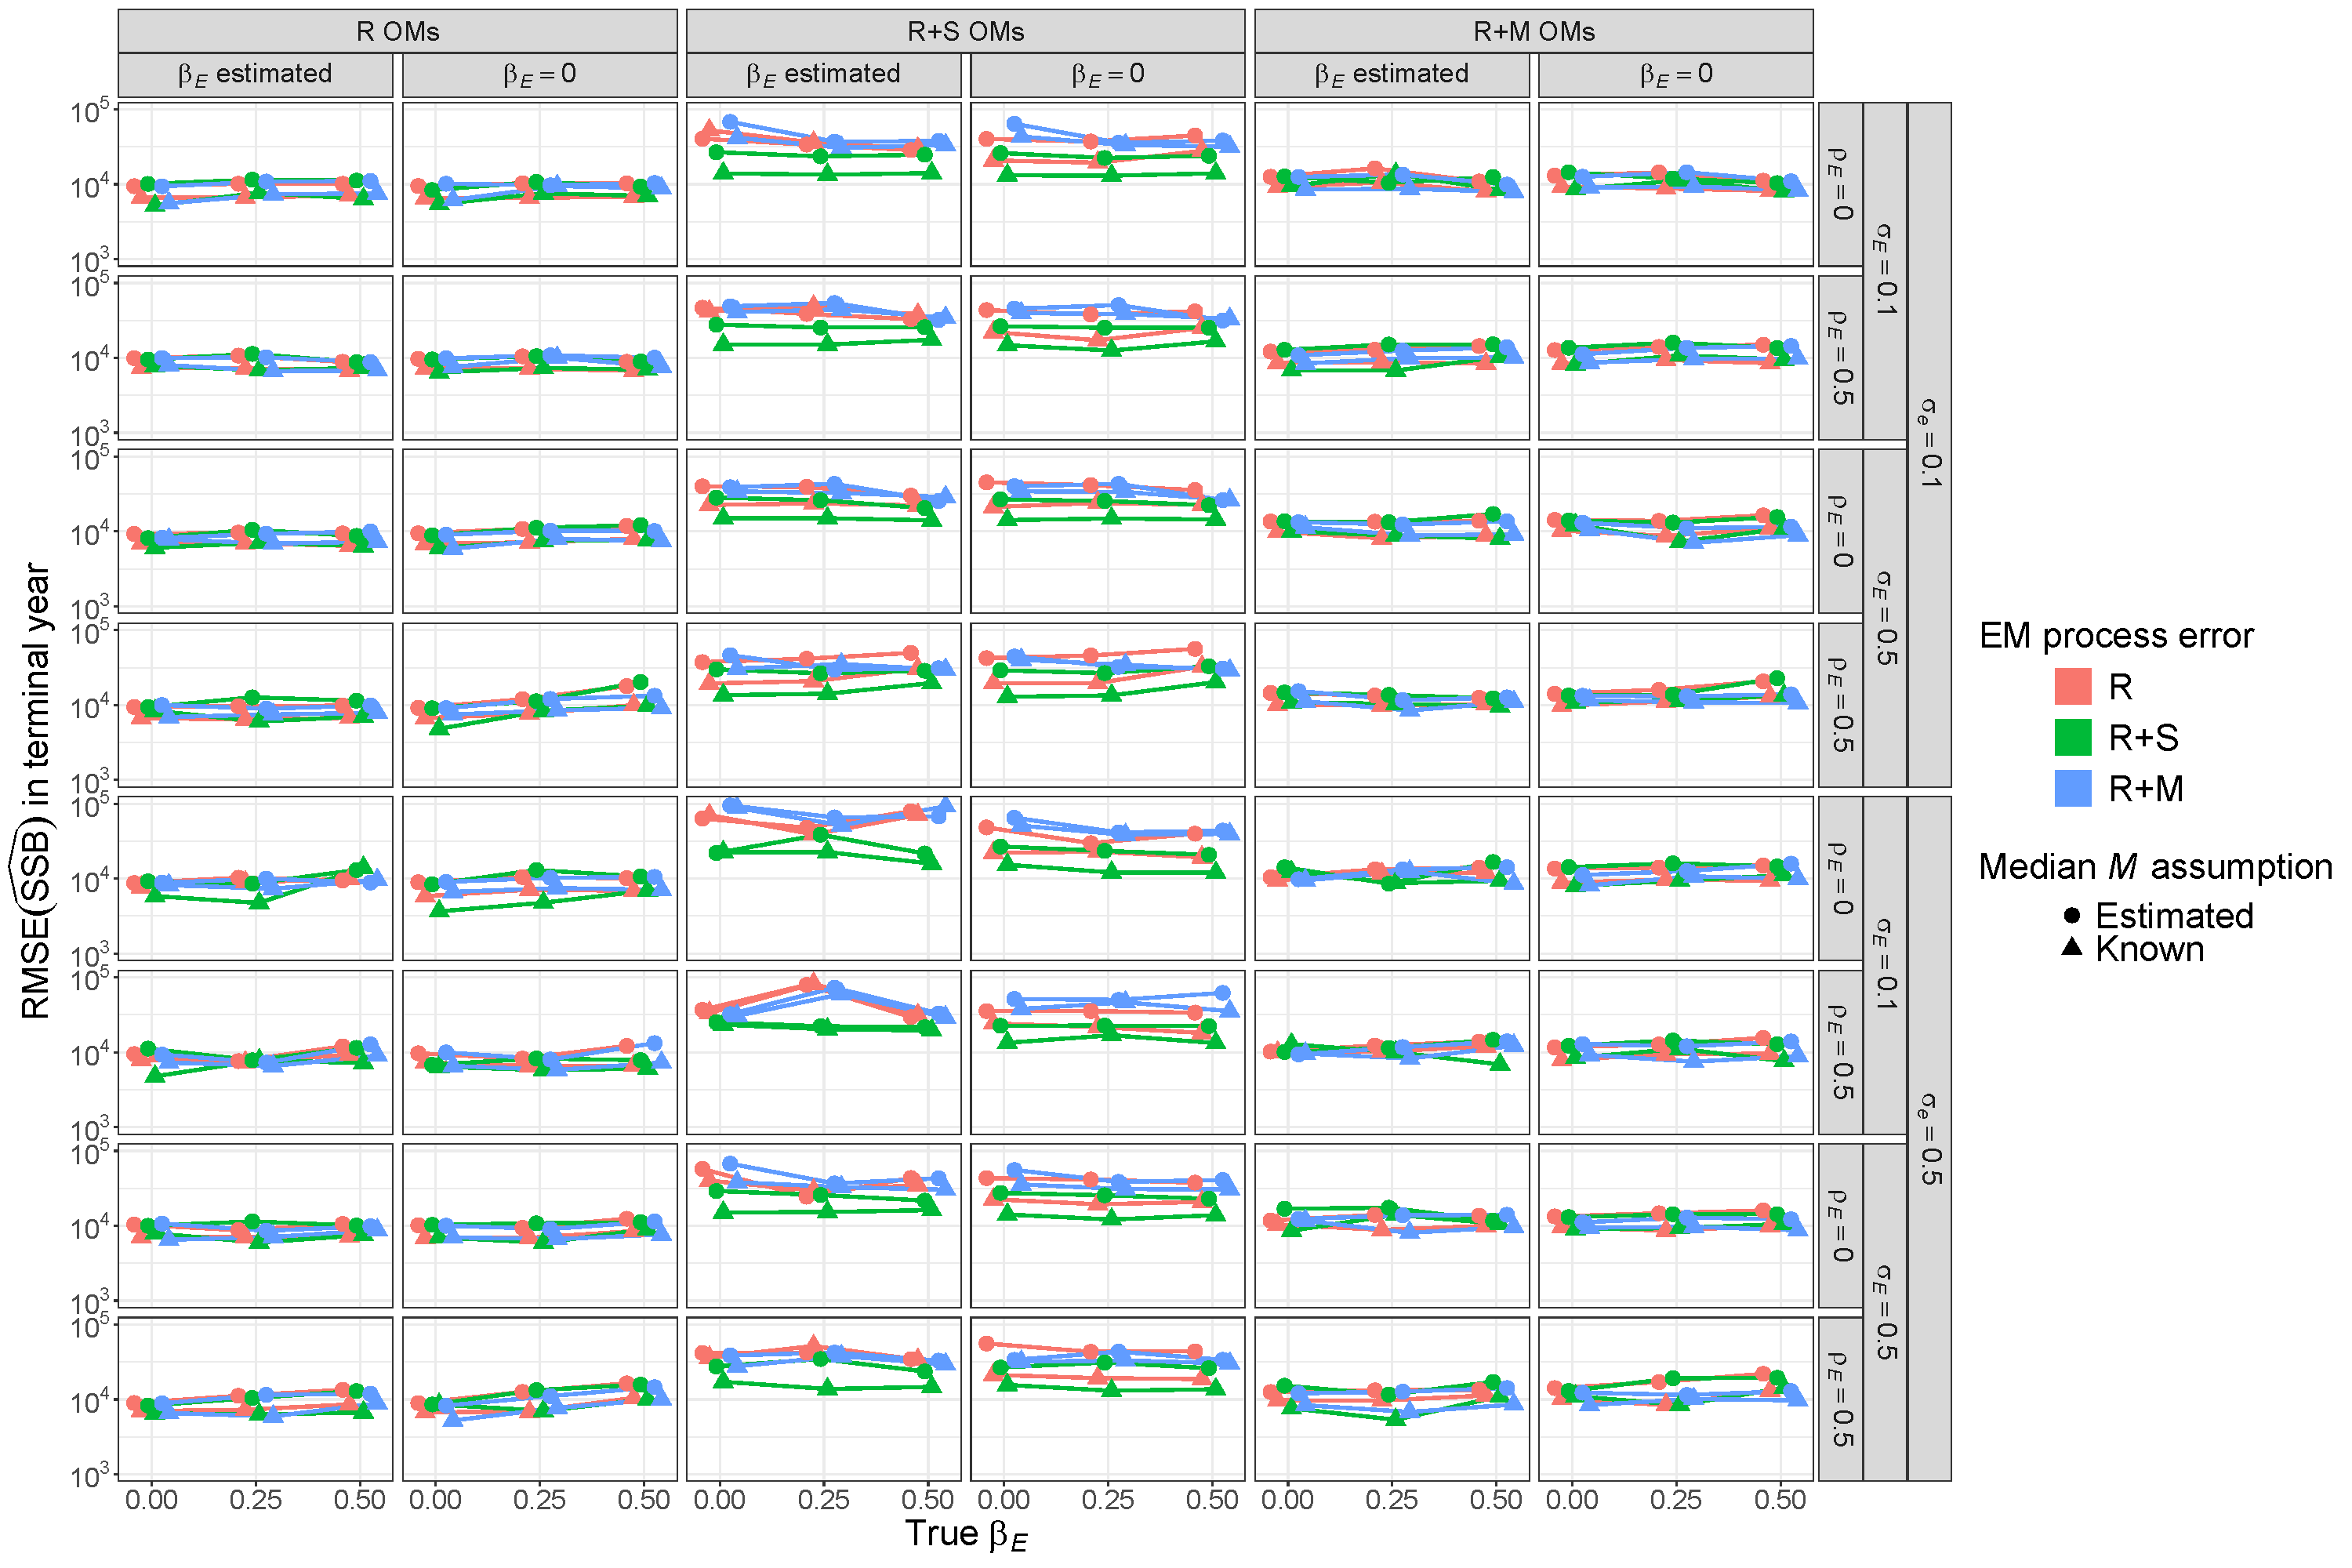
\includegraphics[height = \textheight]{terminal_year_ssb_rmse_main}
%DIFDELCMD < %%%
\DIFdelendFL \DIFaddbeginFL 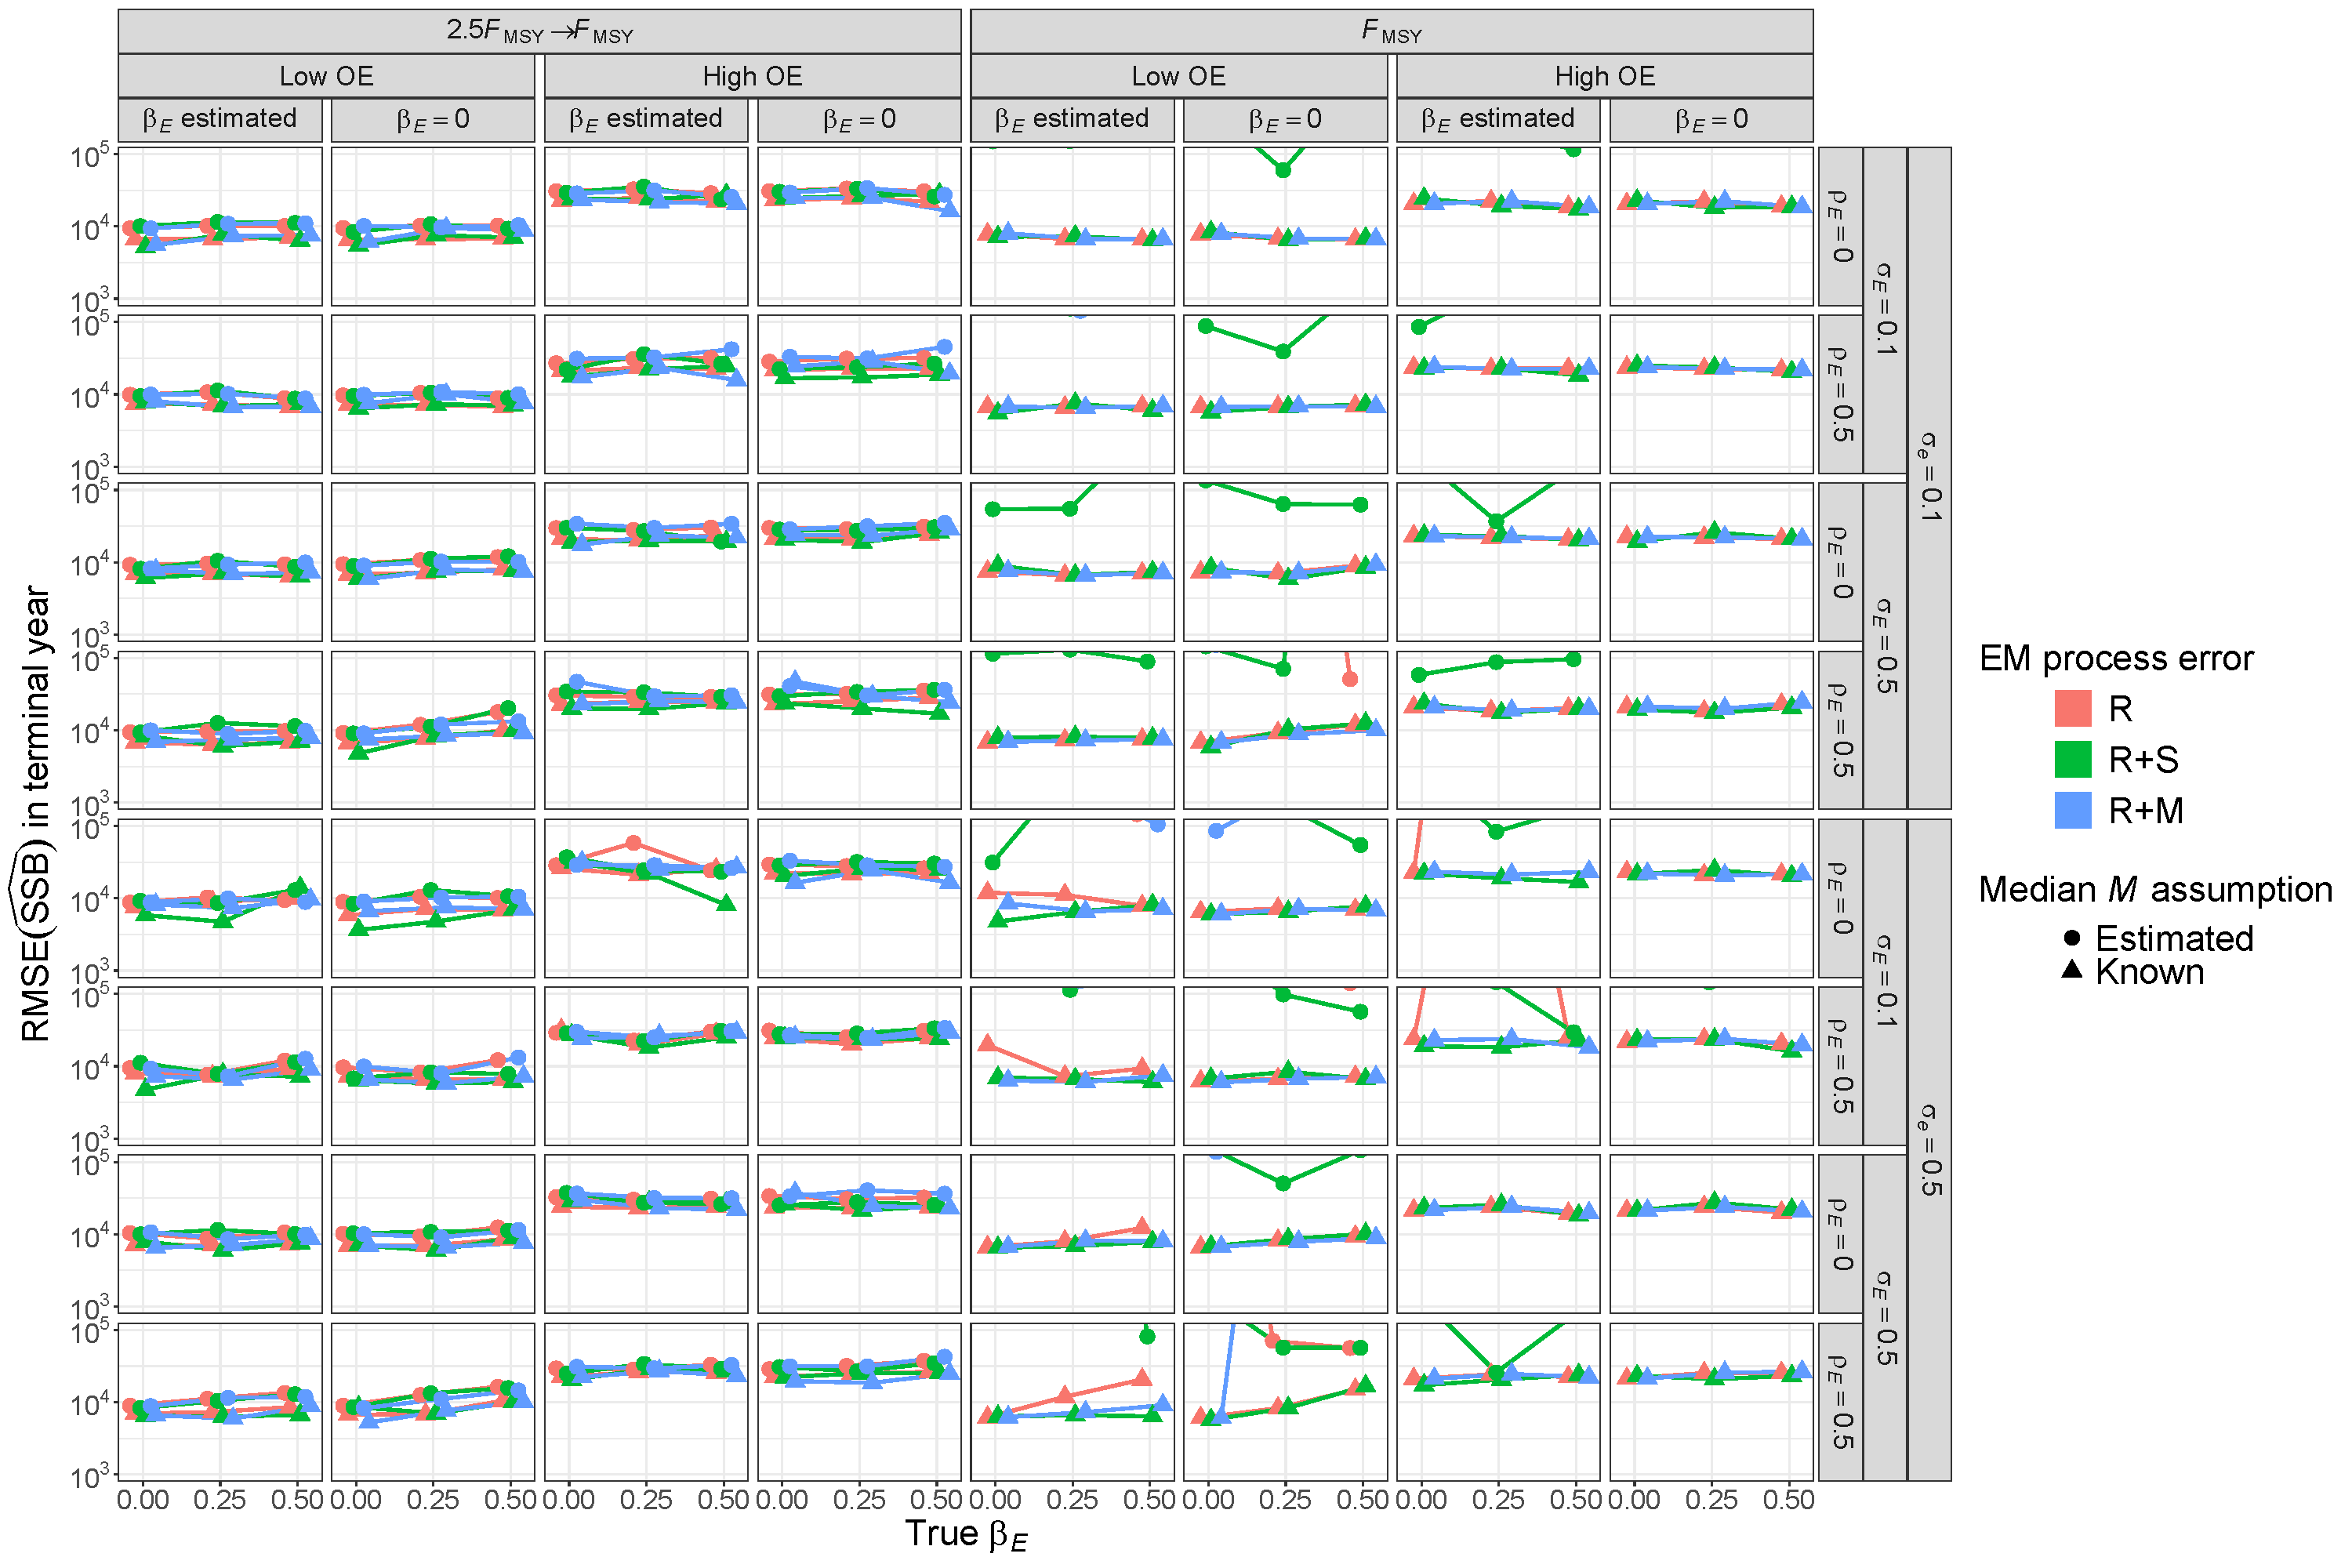
\includegraphics[height = \textheight]{terminal_year_ssb_rmse_Rom}
\DIFaddendFL \end{center}
\caption{\DIFdelbeginFL \DIFdelFL{Root mean square error (}\DIFdelendFL \DIFaddbeginFL \DIFaddFL{For R OMs, }\DIFaddendFL RMSE \DIFdelbeginFL \DIFdelFL{) }\DIFdelendFL of estimates of \DIFdelbeginFL \DIFdelFL{spawning stock biomass }\DIFdelendFL \DIFaddbeginFL \DIFaddFL{SSB }\DIFaddendFL in the terminal year for EMs with alternative process error assumptions, treatment of covariate effect ($\beta_E = 0$ or estimated), and treatment of median \DIFdelbeginFL \DIFdelFL{natural mortality }\DIFdelendFL \DIFaddbeginFL \DIFaddFL{$M$ }\DIFaddendFL parameter ($\beta_M$ estimated or known).\DIFdelbeginFL \DIFdelFL{All OMs had low population observation error and contrast in fishing mortality.}\DIFdelendFL }\DIFdelbeginFL %DIFDELCMD < \label{terminal_ssb_rmse}
%DIFDELCMD < %%%
\DIFdelendFL \DIFaddbeginFL \label{terminal_ssb_rmse_Rom}
\DIFaddendFL \end{figure}
\end{landscape}

\begin{landscape}
\begin{figure}
\begin{center}
\DIFdelbeginFL %DIFDELCMD < 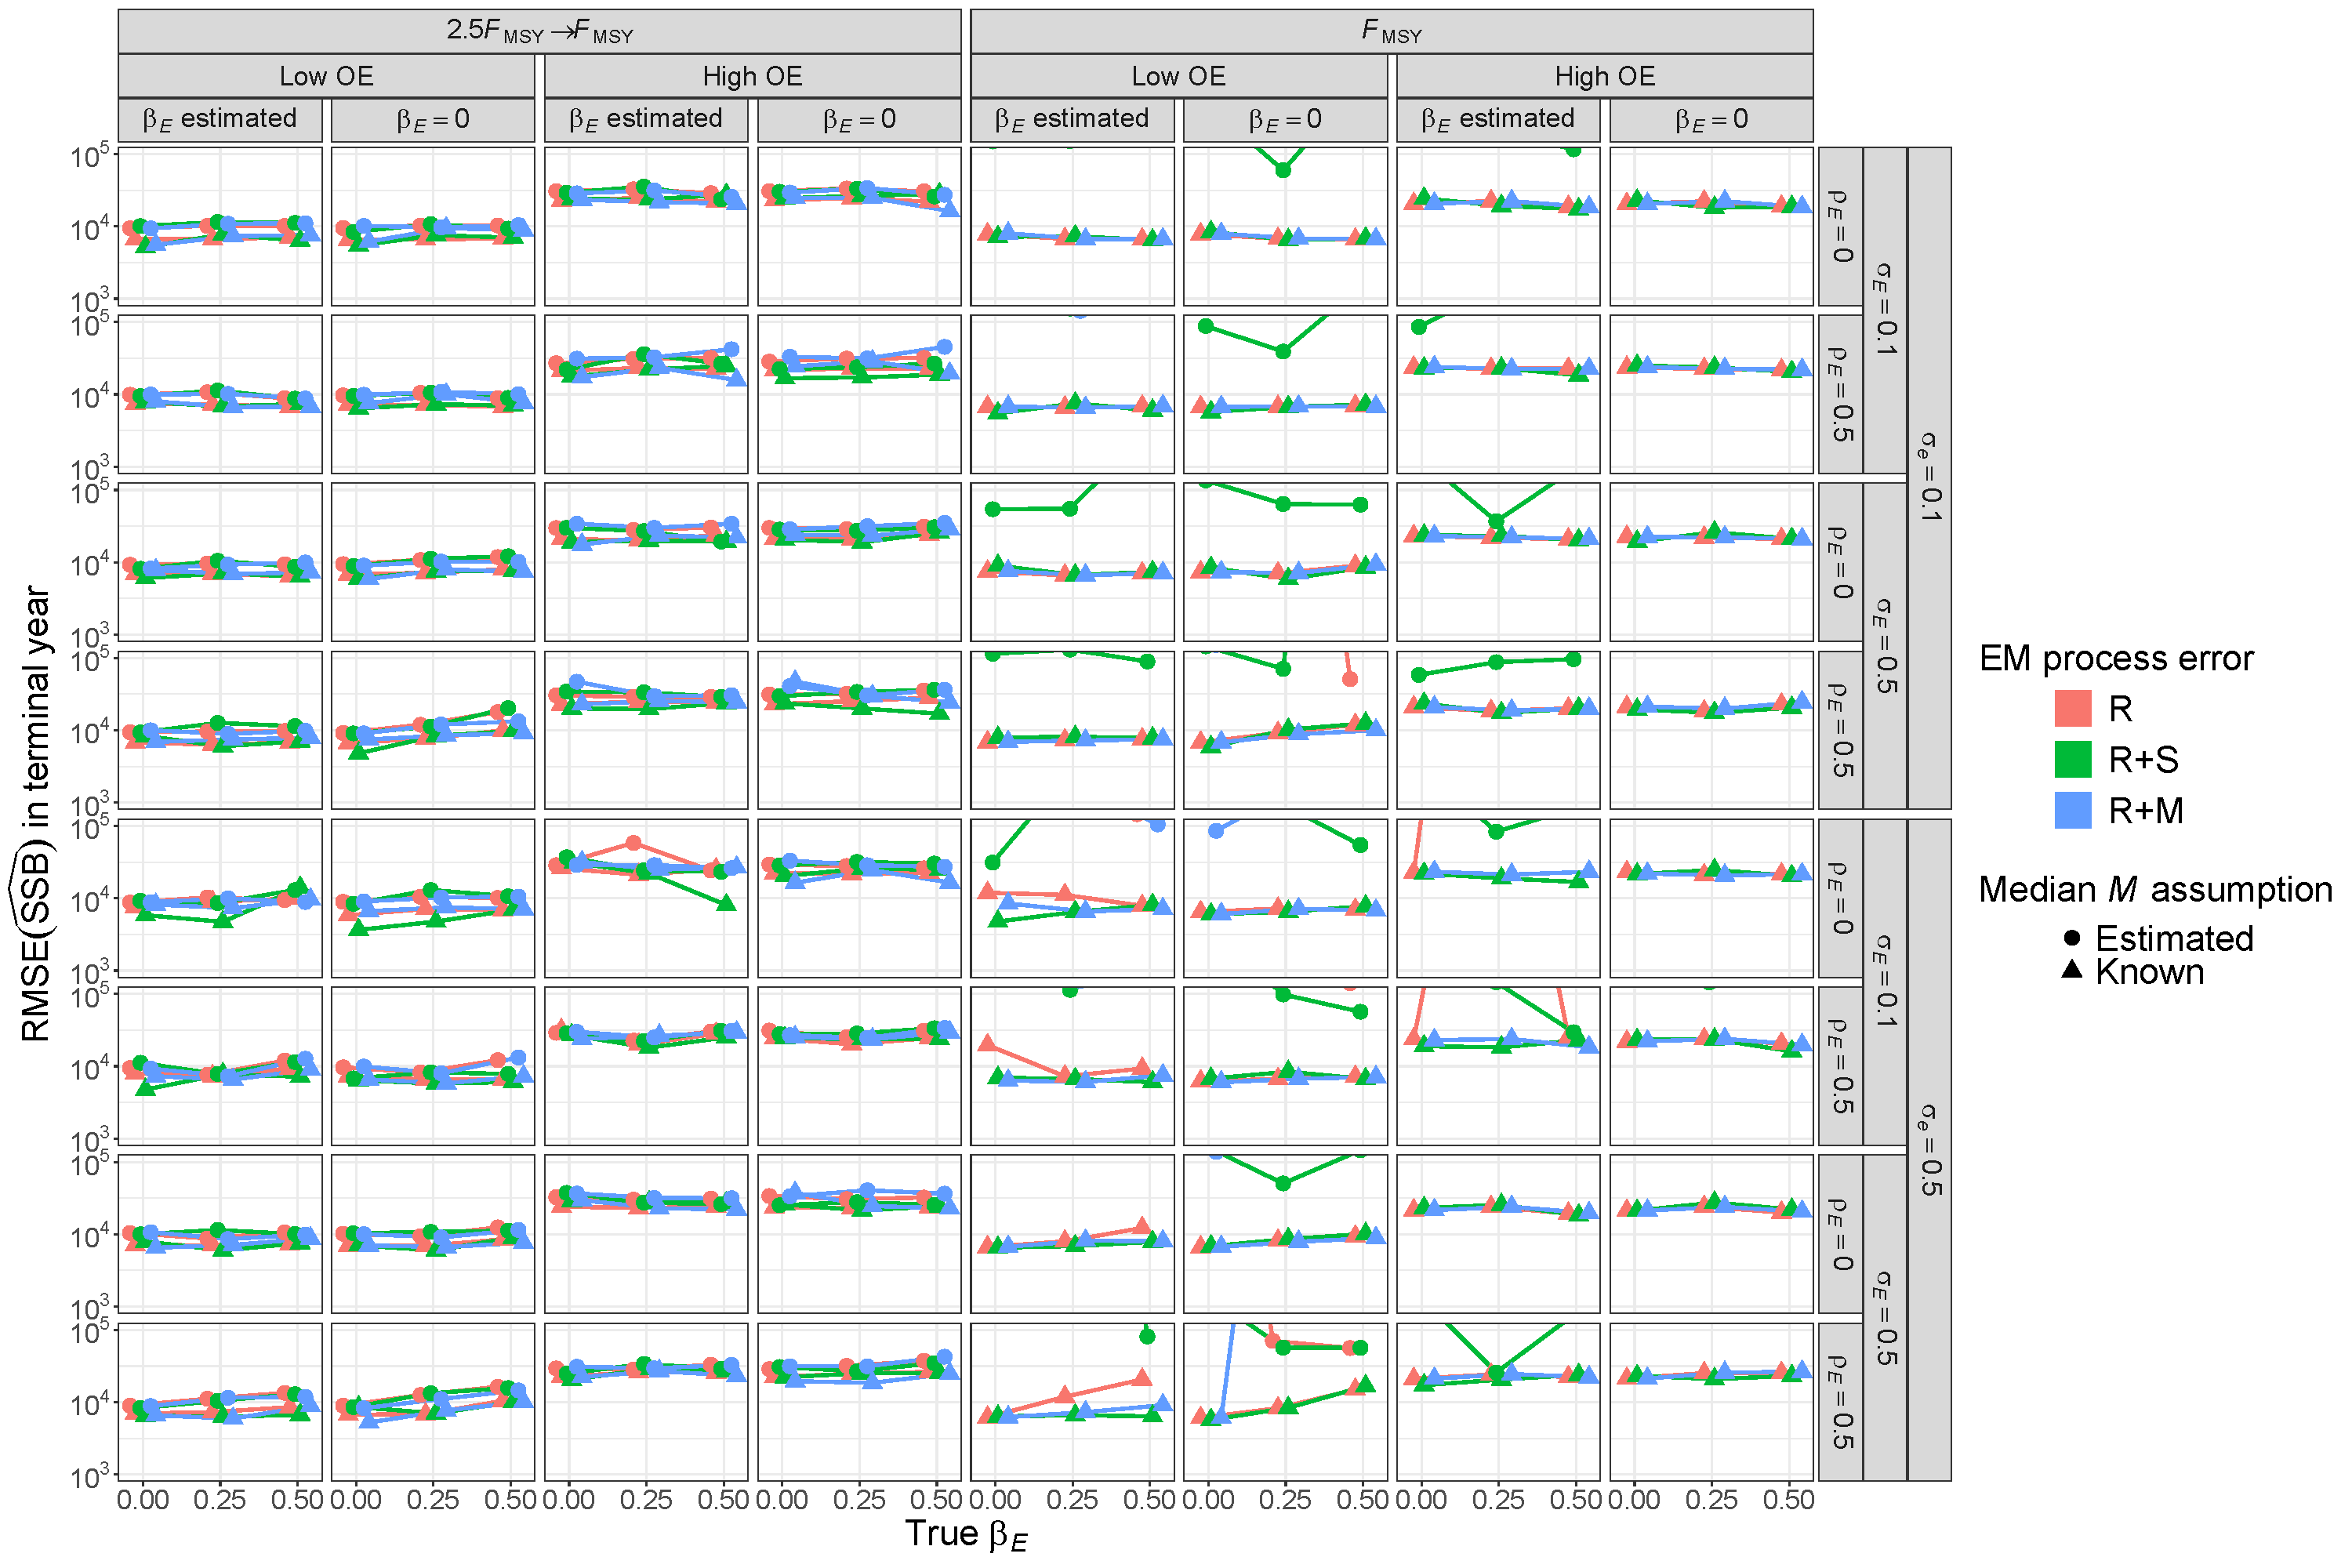
\includegraphics[height = \textheight]{terminal_year_ssb_rmse_Rom}
%DIFDELCMD < %%%
\DIFdelendFL \DIFaddbeginFL 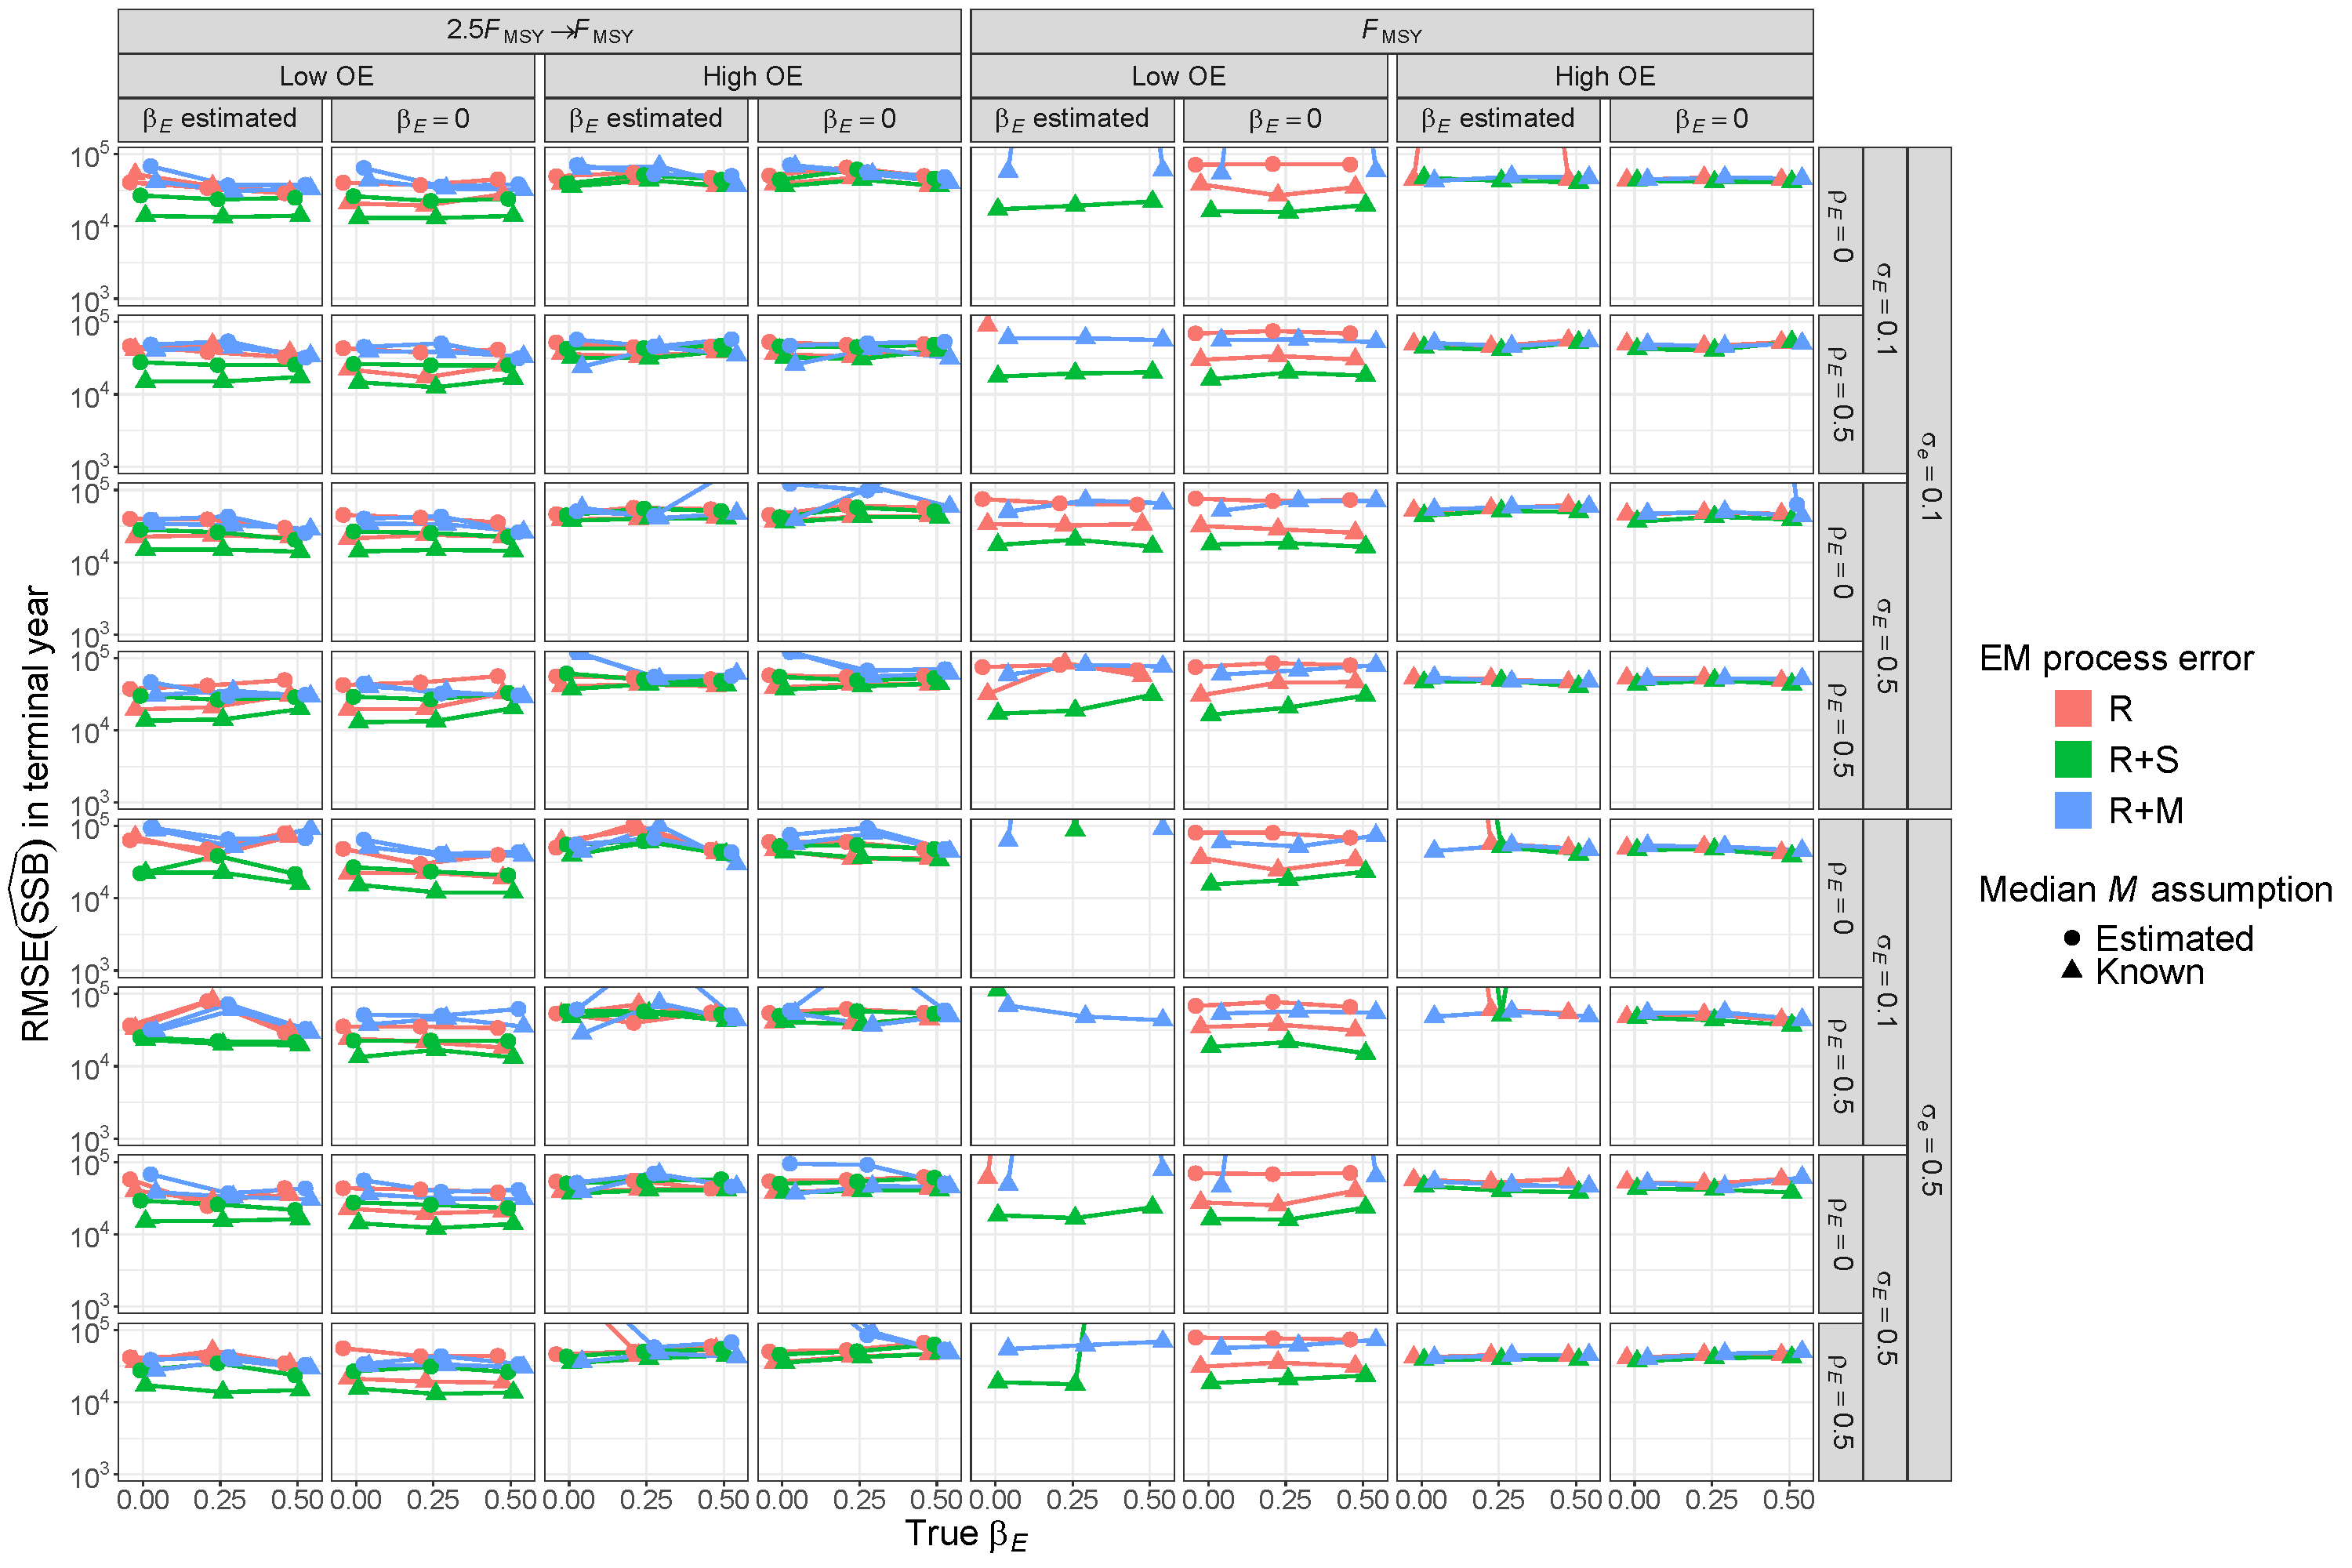
\includegraphics[height = \textheight]{terminal_year_ssb_rmse_RSom}
\DIFaddendFL \end{center}
\caption{For R\DIFaddbeginFL \DIFaddFL{+S }\DIFaddendFL OMs, \DIFdelbeginFL \DIFdelFL{root mean square error (}\DIFdelendFL RMSE \DIFdelbeginFL \DIFdelFL{) }\DIFdelendFL of estimates of \DIFdelbeginFL \DIFdelFL{spawning stock biomass }\DIFdelendFL \DIFaddbeginFL \DIFaddFL{SSB }\DIFaddendFL in the terminal year for EMs with alternative process error assumptions, treatment of covariate effect ($\beta_E = 0$ or estimated), and treatment of median \DIFdelbeginFL \DIFdelFL{natural mortality }\DIFdelendFL \DIFaddbeginFL \DIFaddFL{$M$ }\DIFaddendFL parameter ($\beta_M$ estimated or known).}\DIFdelbeginFL %DIFDELCMD < \label{terminal_ssb_rmse_Rom}
%DIFDELCMD < %%%
\DIFdelendFL \DIFaddbeginFL \label{terminal_ssb_rmse_RSom}
\DIFaddendFL \end{figure}
\end{landscape}

\begin{landscape}
\begin{figure}
\begin{center}
\DIFdelbeginFL %DIFDELCMD < 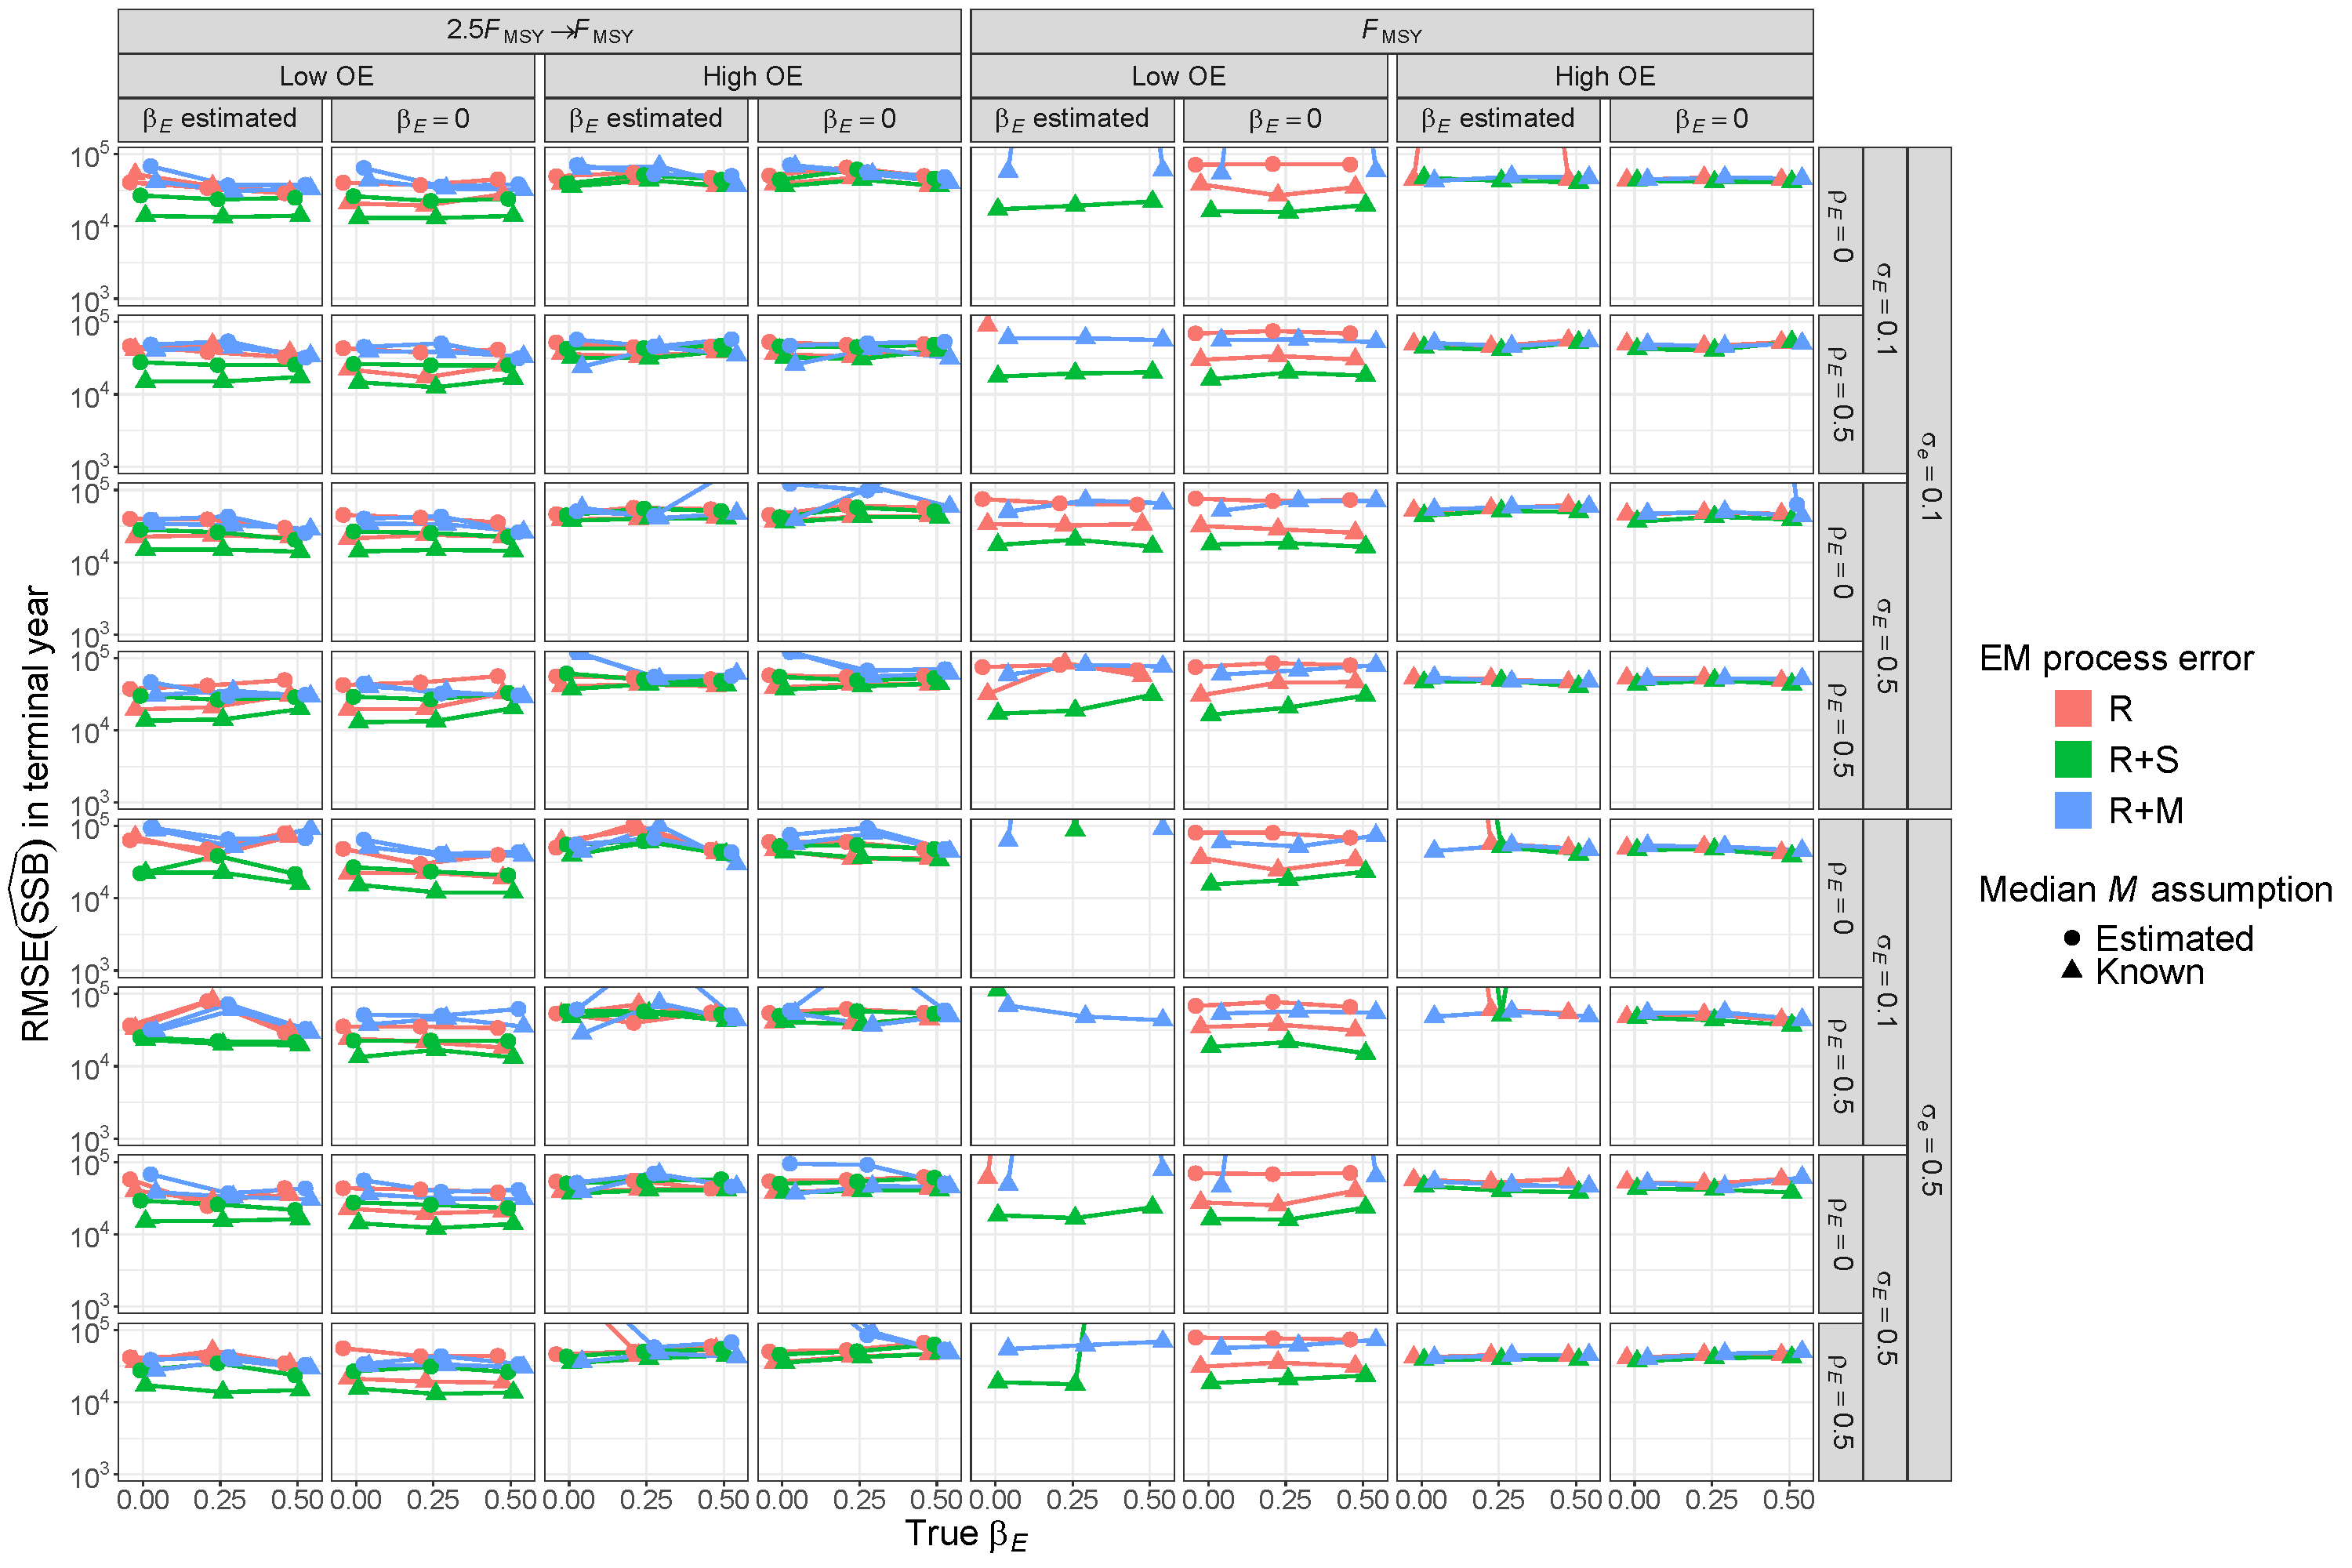
\includegraphics[height = \textheight]{terminal_year_ssb_rmse_RSom}
%DIFDELCMD < %%%
\DIFdelendFL \DIFaddbeginFL 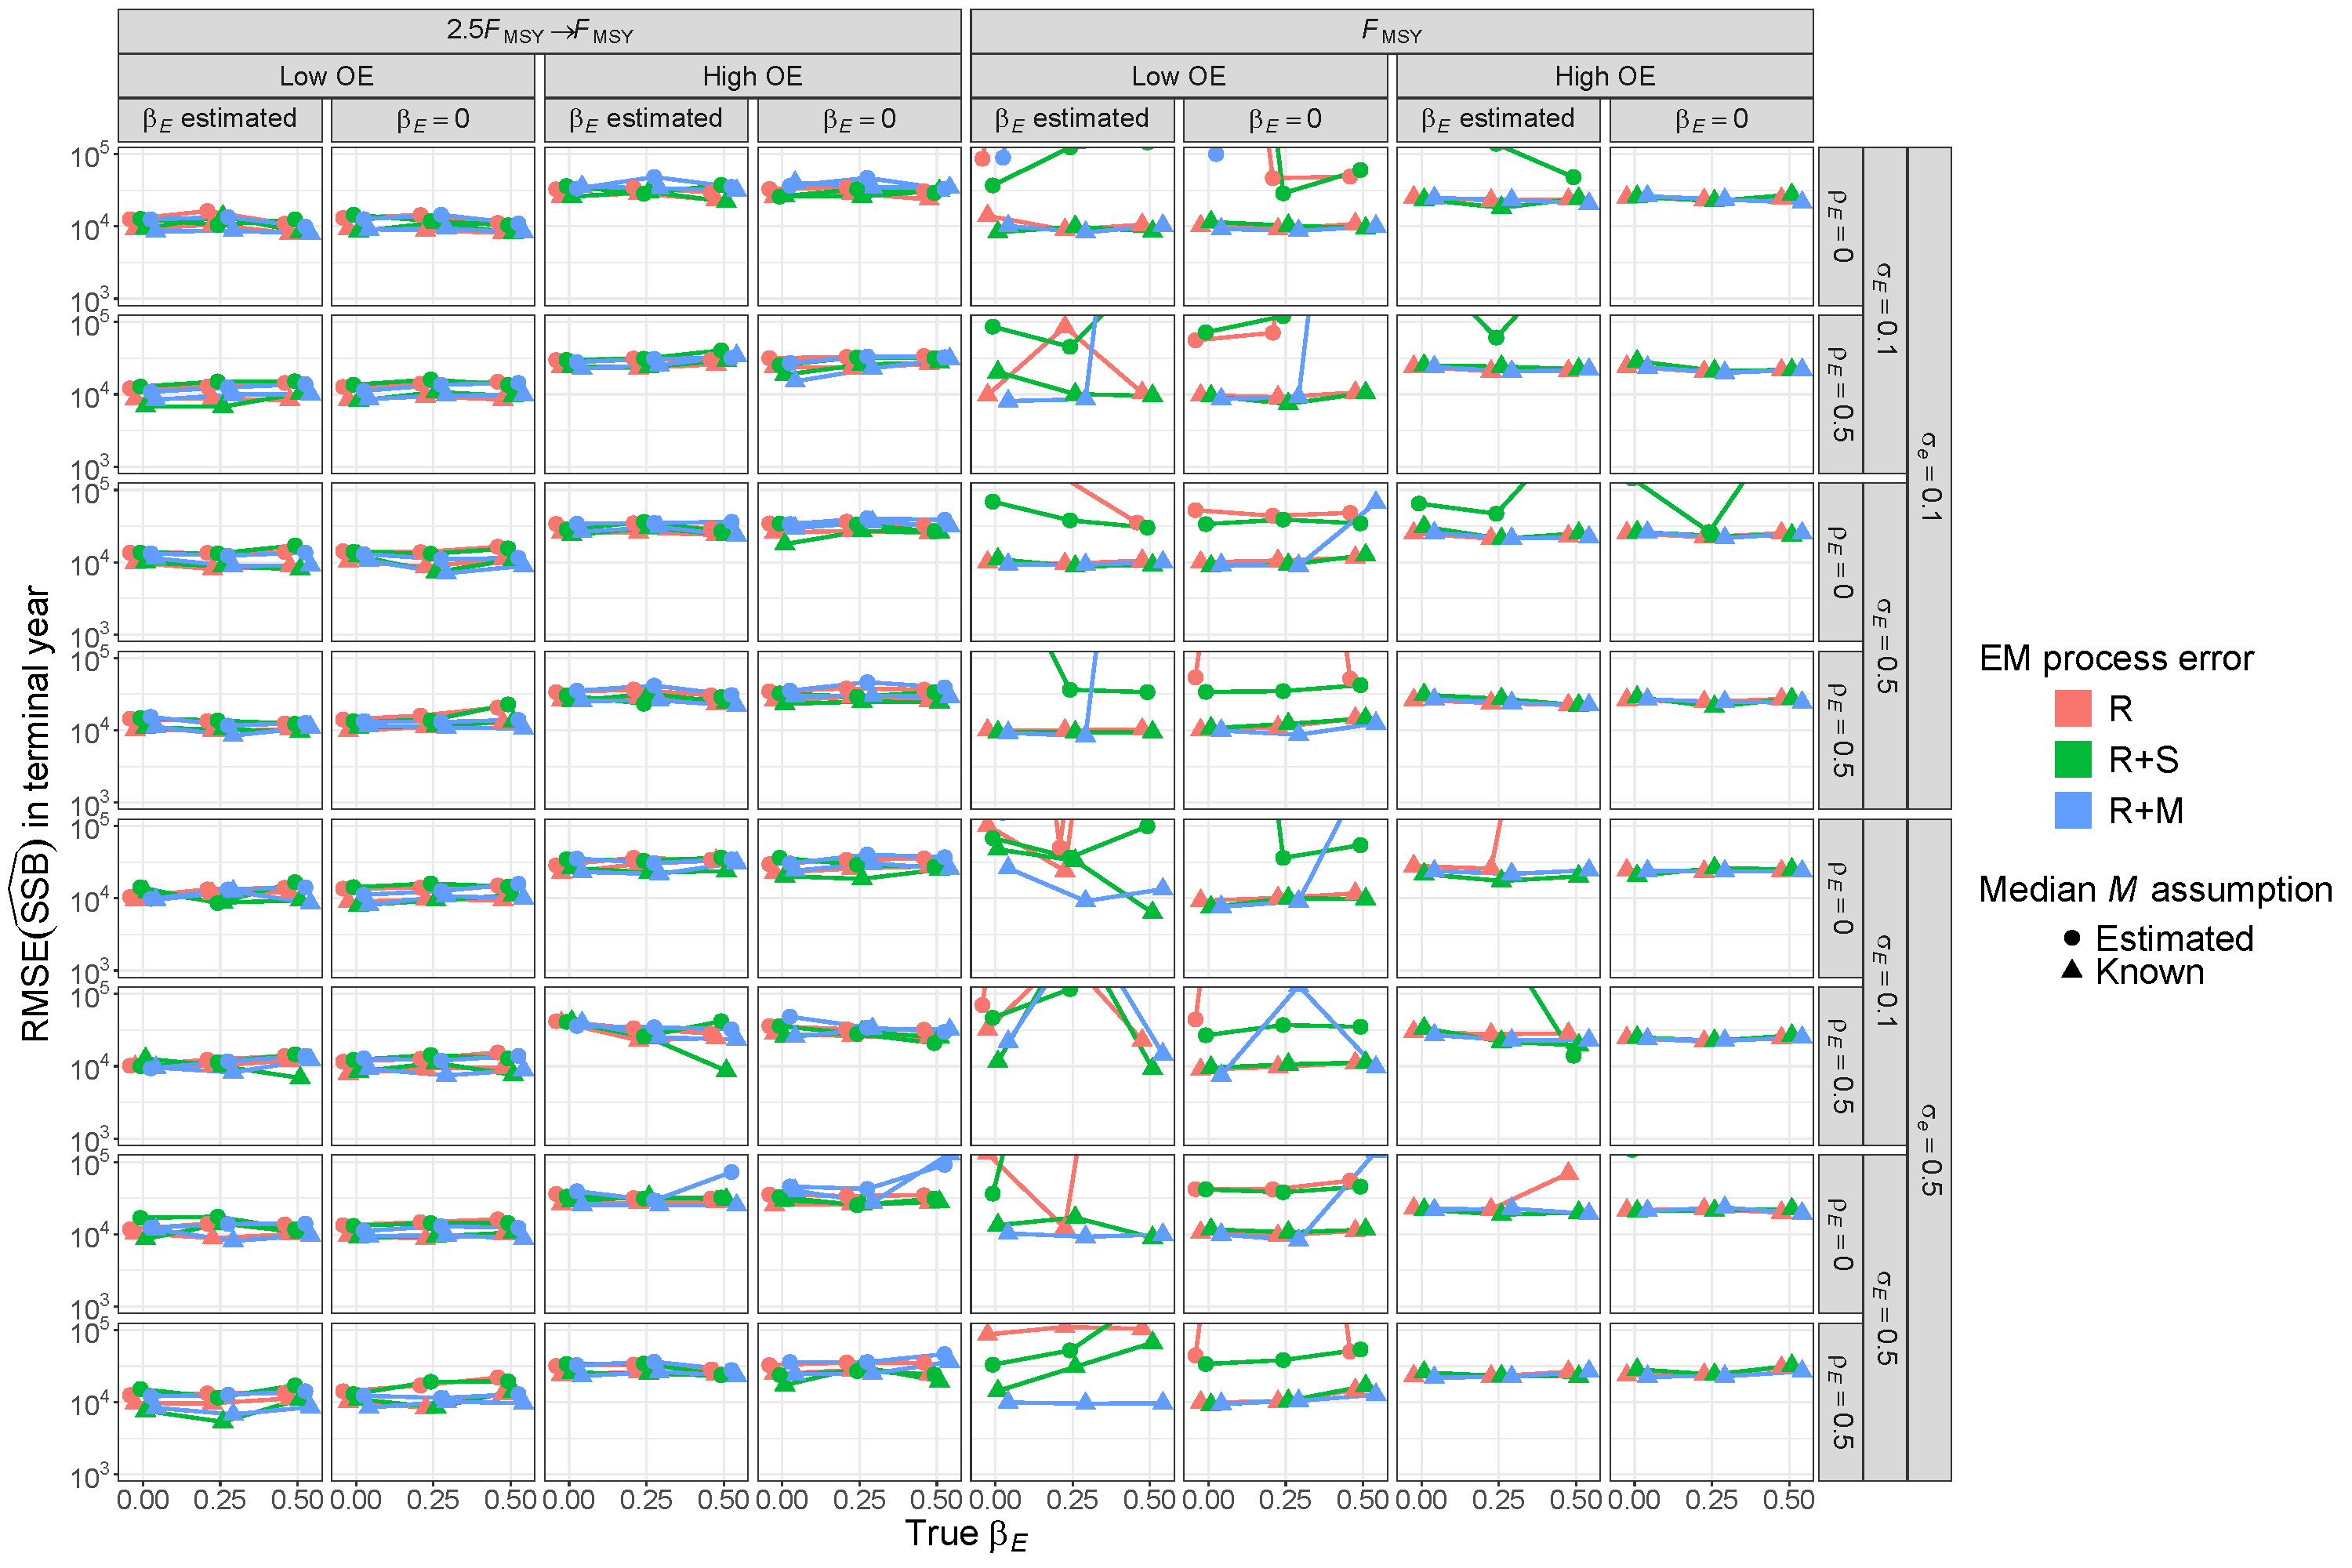
\includegraphics[height = \textheight]{terminal_year_ssb_rmse_RMom}
\DIFaddendFL \end{center}
\caption{For R+\DIFdelbeginFL \DIFdelFL{S }\DIFdelendFL \DIFaddbeginFL \DIFaddFL{M }\DIFaddendFL OMs, \DIFdelbeginFL \DIFdelFL{root mean square error (}\DIFdelendFL RMSE \DIFdelbeginFL \DIFdelFL{) }\DIFdelendFL of estimates of \DIFdelbeginFL \DIFdelFL{spawning stock biomass }\DIFdelendFL \DIFaddbeginFL \DIFaddFL{SSB }\DIFaddendFL in the terminal year for EMs with alternative process error assumptions, treatment of covariate effect ($\beta_E = 0$ or estimated), and treatment of median \DIFdelbeginFL \DIFdelFL{natural mortality }\DIFdelendFL \DIFaddbeginFL \DIFaddFL{$M$ }\DIFaddendFL parameter ($\beta_M$ estimated or known).}\DIFdelbeginFL %DIFDELCMD < \label{terminal_ssb_rmse_RSom}
%DIFDELCMD < %%%
\DIFdelendFL \DIFaddbeginFL \label{terminal_ssb_rmse_RMom}
\DIFaddendFL \end{figure}
\end{landscape}

\begin{landscape}
\begin{figure}
\begin{center}
\DIFdelbeginFL %DIFDELCMD < 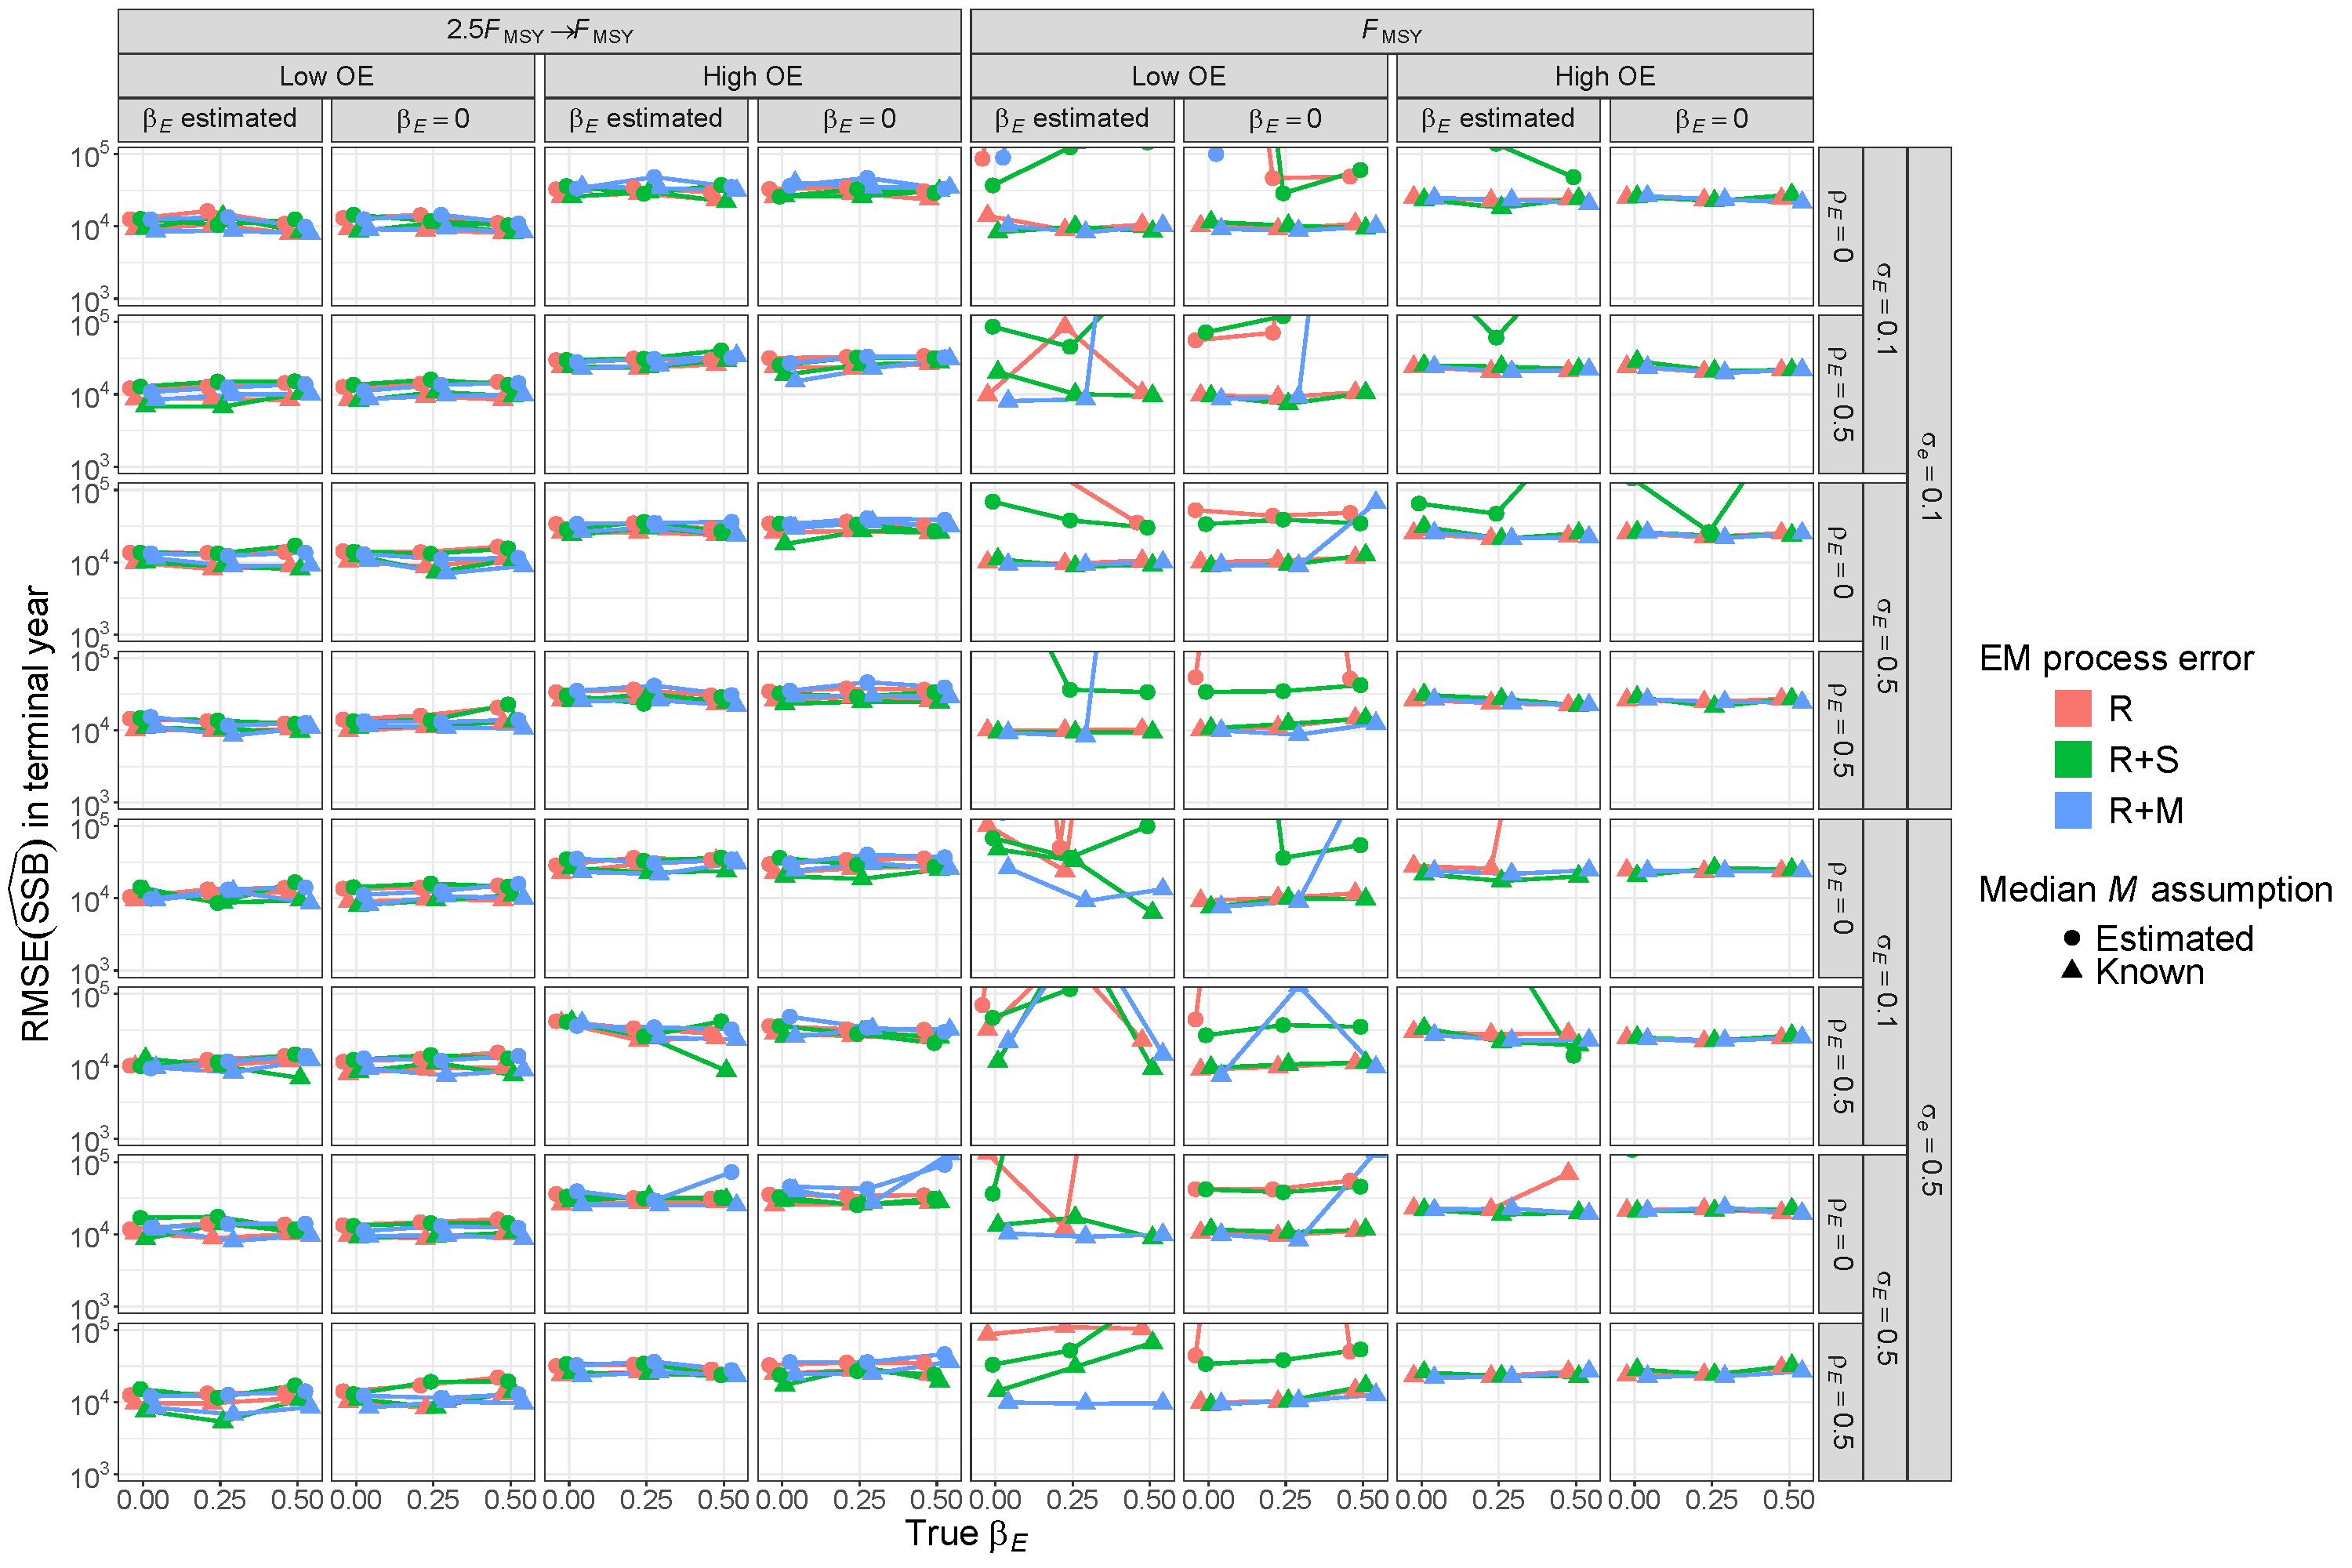
\includegraphics[height = \textheight]{terminal_year_ssb_rmse_RMom}
%DIFDELCMD < %%%
\DIFdelendFL \DIFaddbeginFL 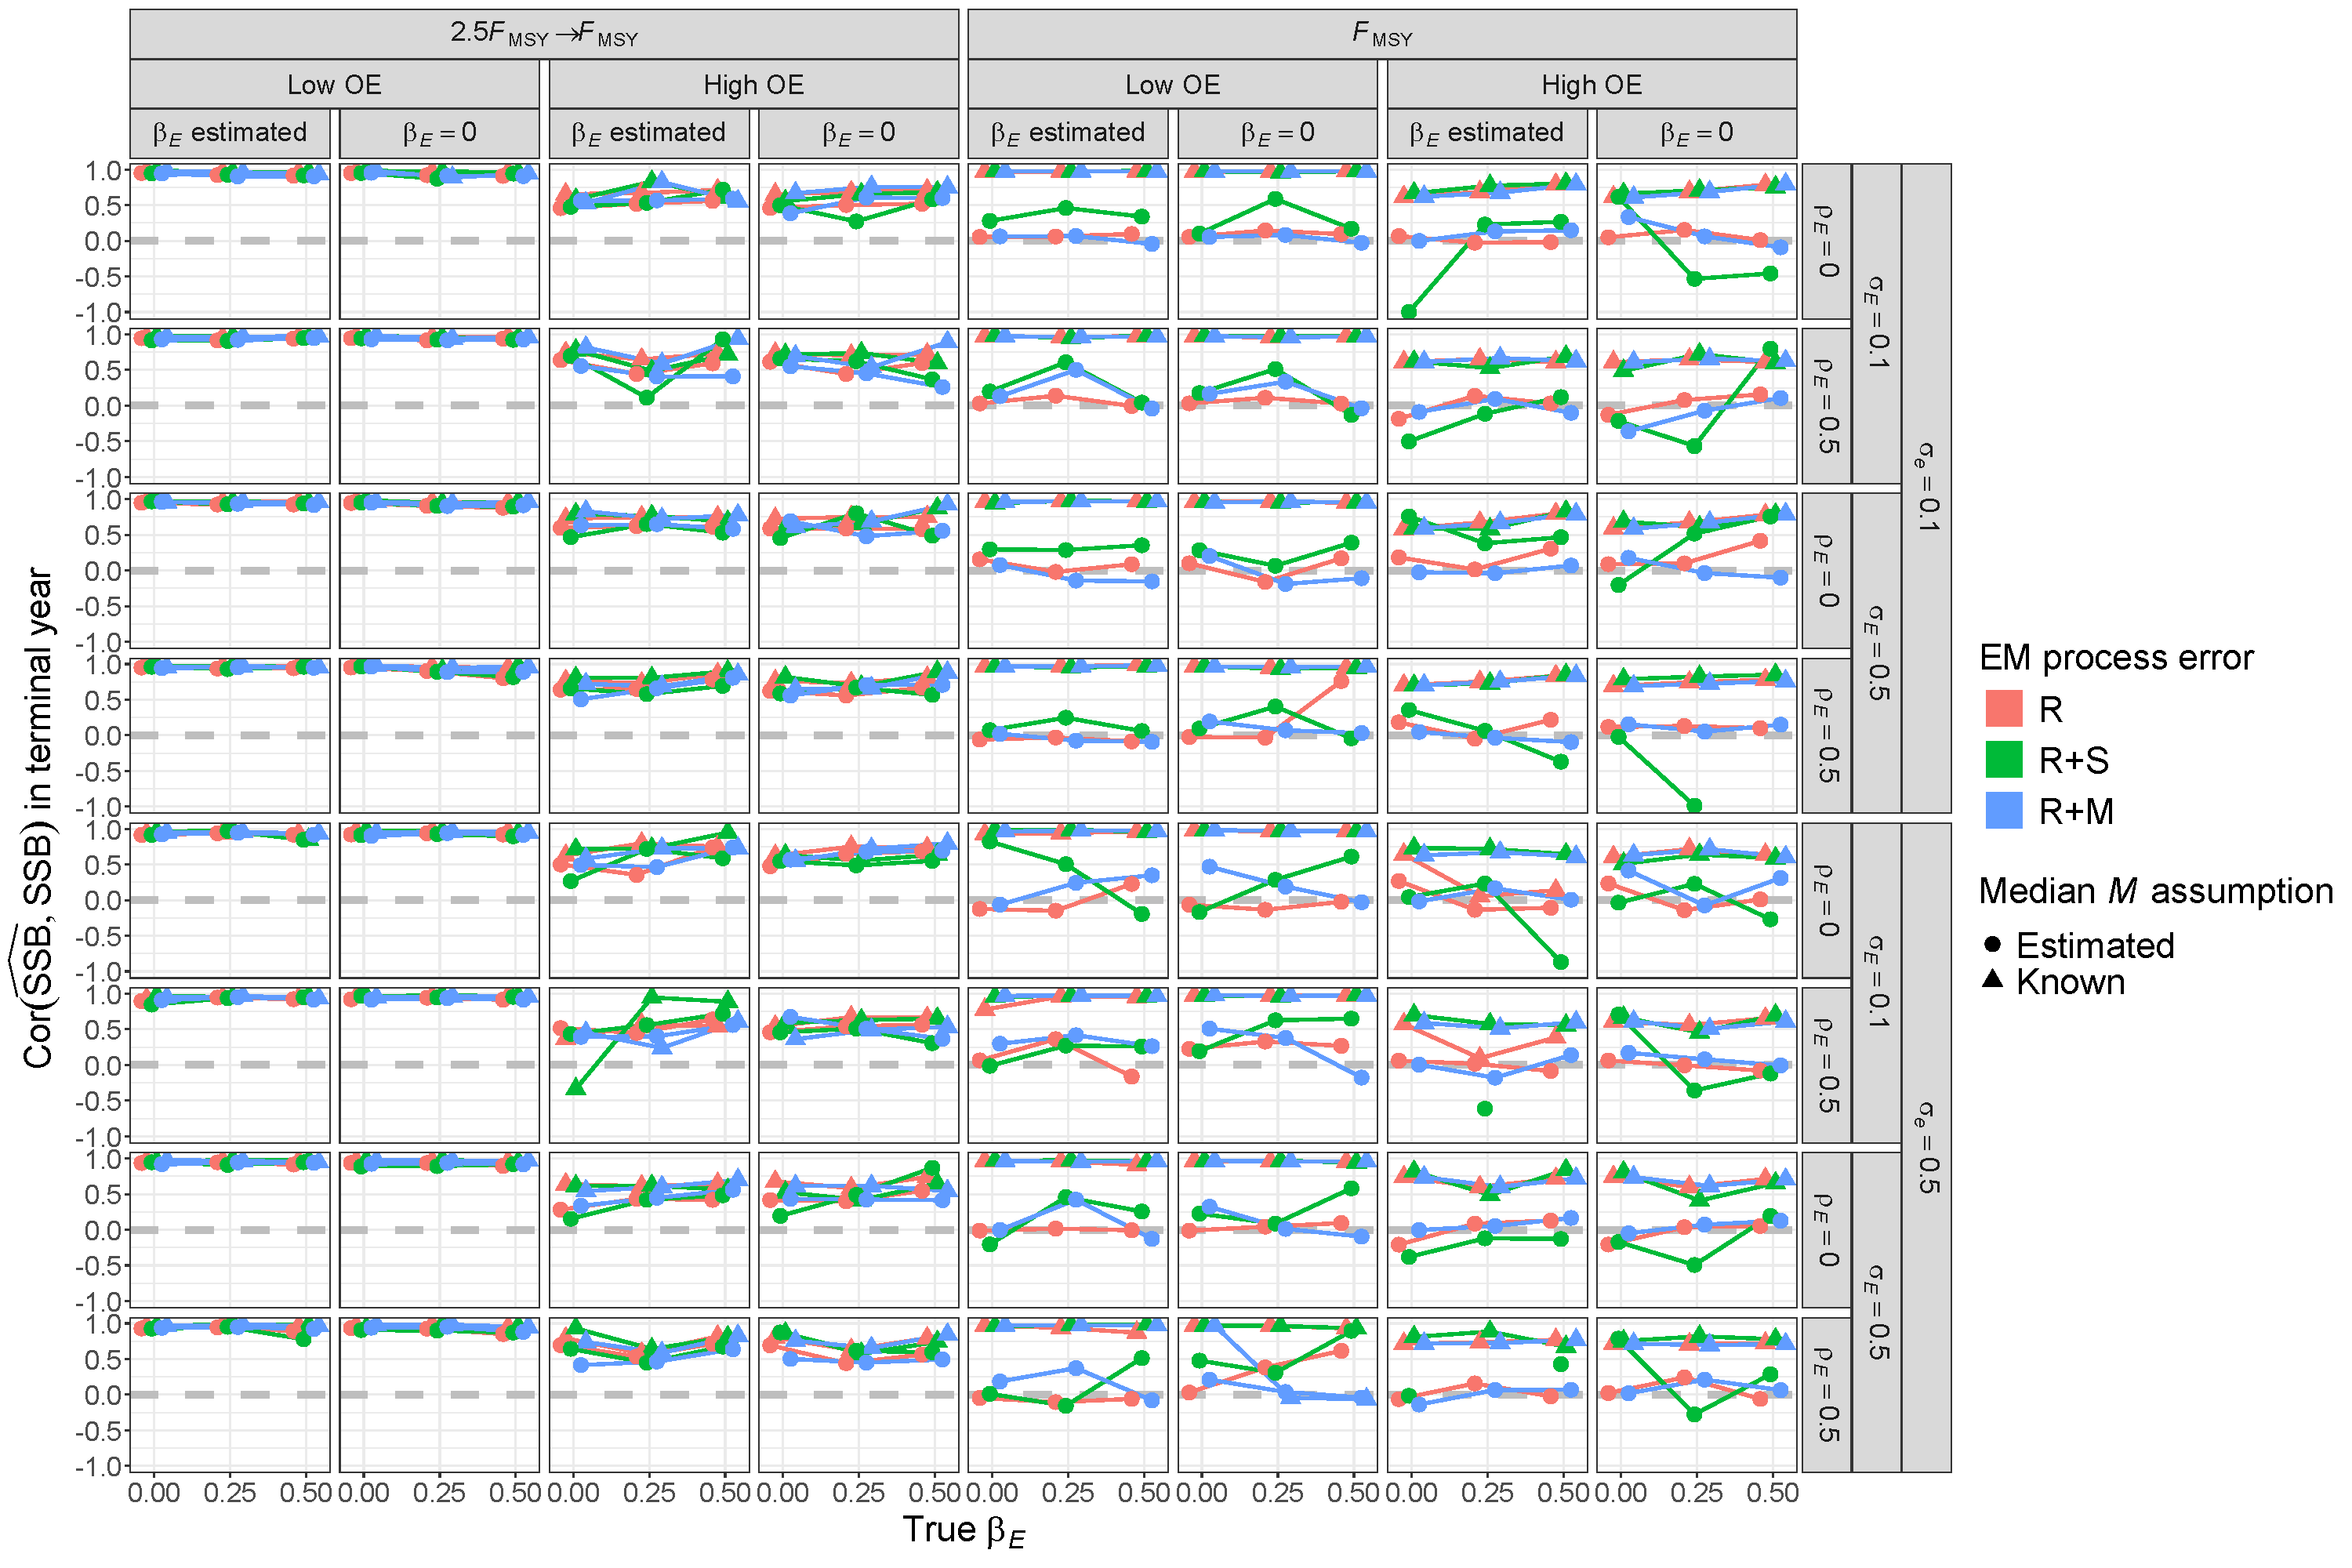
\includegraphics[height = \textheight]{terminal_year_ssb_corr_Rom}
\DIFaddendFL \end{center}
\caption{For R \DIFdelbeginFL \DIFdelFL{+M }\DIFdelendFL OMs, \DIFdelbeginFL \DIFdelFL{root mean square error (RMSE) }\DIFdelendFL \DIFaddbeginFL \DIFaddFL{correlation }\DIFaddendFL of estimates \DIFaddbeginFL \DIFaddFL{and true values }\DIFaddendFL of \DIFdelbeginFL \DIFdelFL{spawning stock biomass in the }\DIFdelendFL terminal year \DIFaddbeginFL \DIFaddFL{SSB }\DIFaddendFL for EMs with alternative process error assumptions, treatment of covariate effect ($\beta_E = 0$ or estimated), and treatment of median \DIFdelbeginFL \DIFdelFL{natural mortality }\DIFdelendFL \DIFaddbeginFL \DIFaddFL{$M$ }\DIFaddendFL parameter ($\beta_M$ estimated or known).}\DIFdelbeginFL %DIFDELCMD < \label{terminal_ssb_rmse_RMom}
%DIFDELCMD < %%%
\DIFdelendFL \DIFaddbeginFL \label{terminal_ssb_corr_Rom}
\DIFaddendFL \end{figure}
\end{landscape}

\DIFdelbegin %DIFDELCMD < \hypertarget{terminal-year-fishing-mortality-bias}{%
%DIFDELCMD < \subsection*{Terminal year fishing mortality bias}\label{terminal-year-fishing-mortality-bias}}
%DIFDELCMD < %%%
\DIFdelend \DIFaddbegin \begin{landscape}
\begin{figure}
\begin{center}
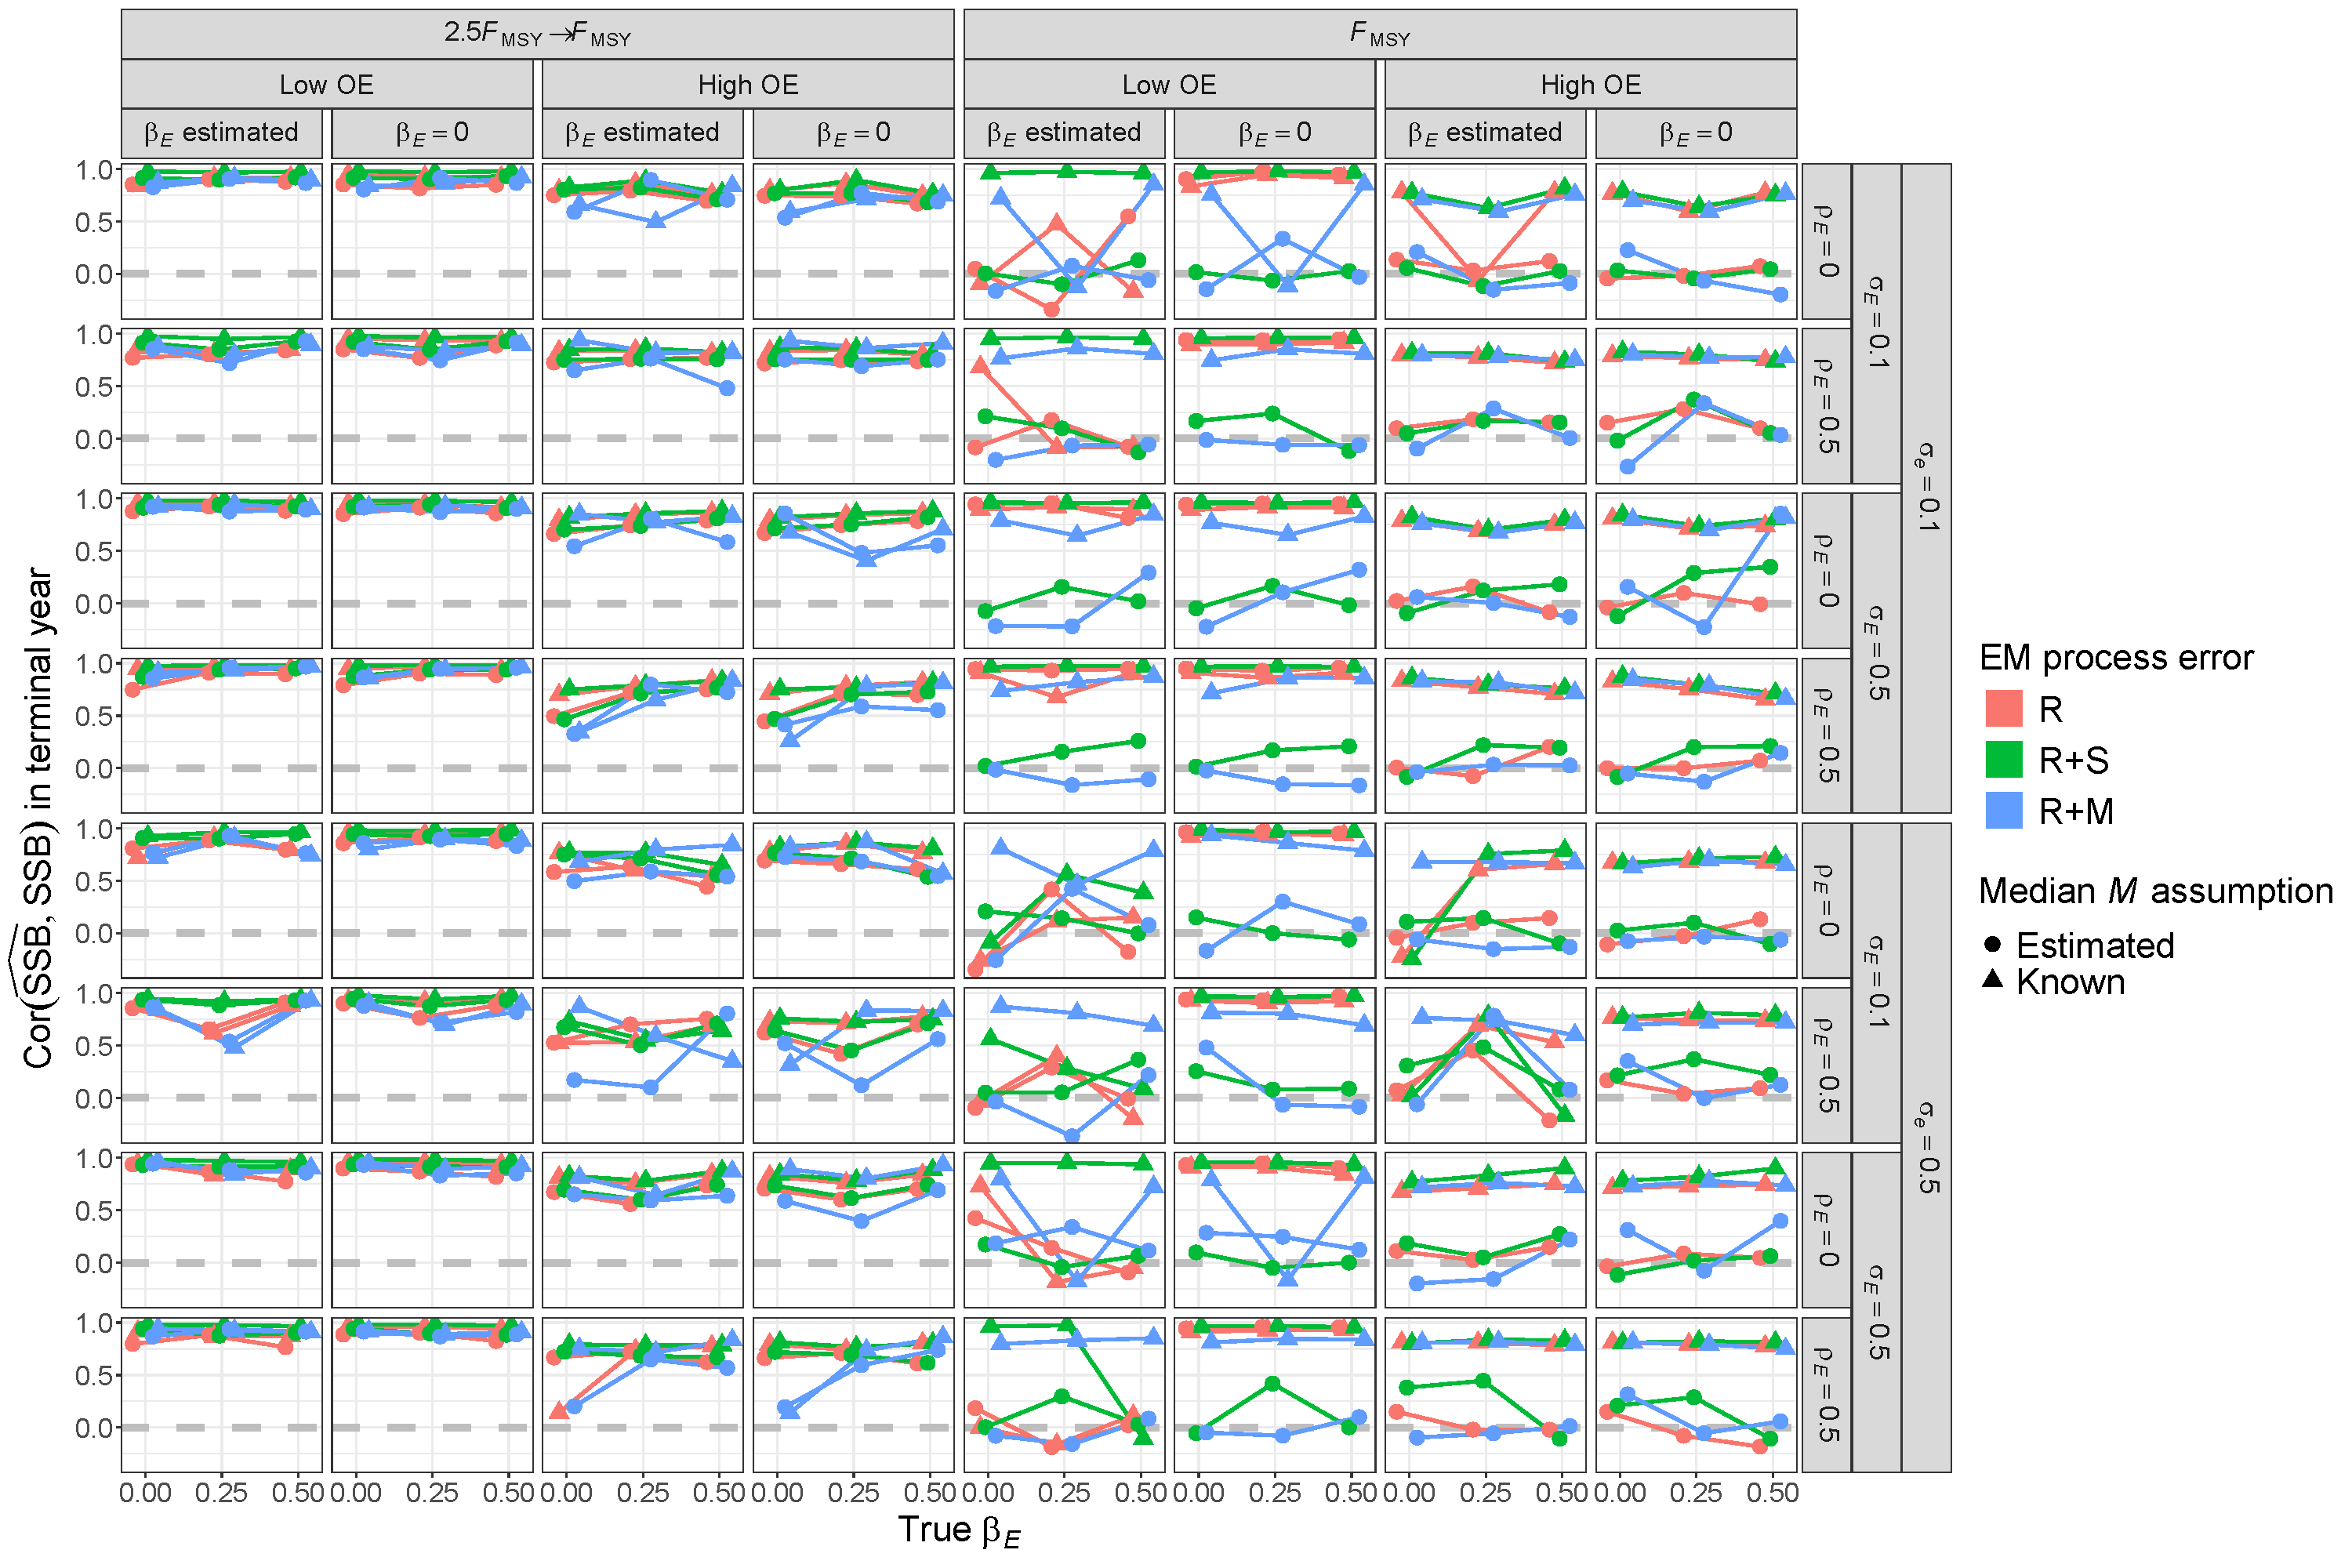
\includegraphics[height = \textheight]{terminal_year_ssb_corr_RSom}
\end{center}
\caption{\DIFaddFL{For R+S OMs, correlation of estimates and true values of terminal year SSB for EMs with alternative process error assumptions, treatment of covariate effect ($\beta_E = 0$ or estimated), and treatment of median $M$ parameter ($\beta_M$ estimated or known).}}\label{terminal_ssb_corr_RSom}
\end{figure}
\end{landscape}

\begin{landscape}
\begin{figure}
\begin{center}
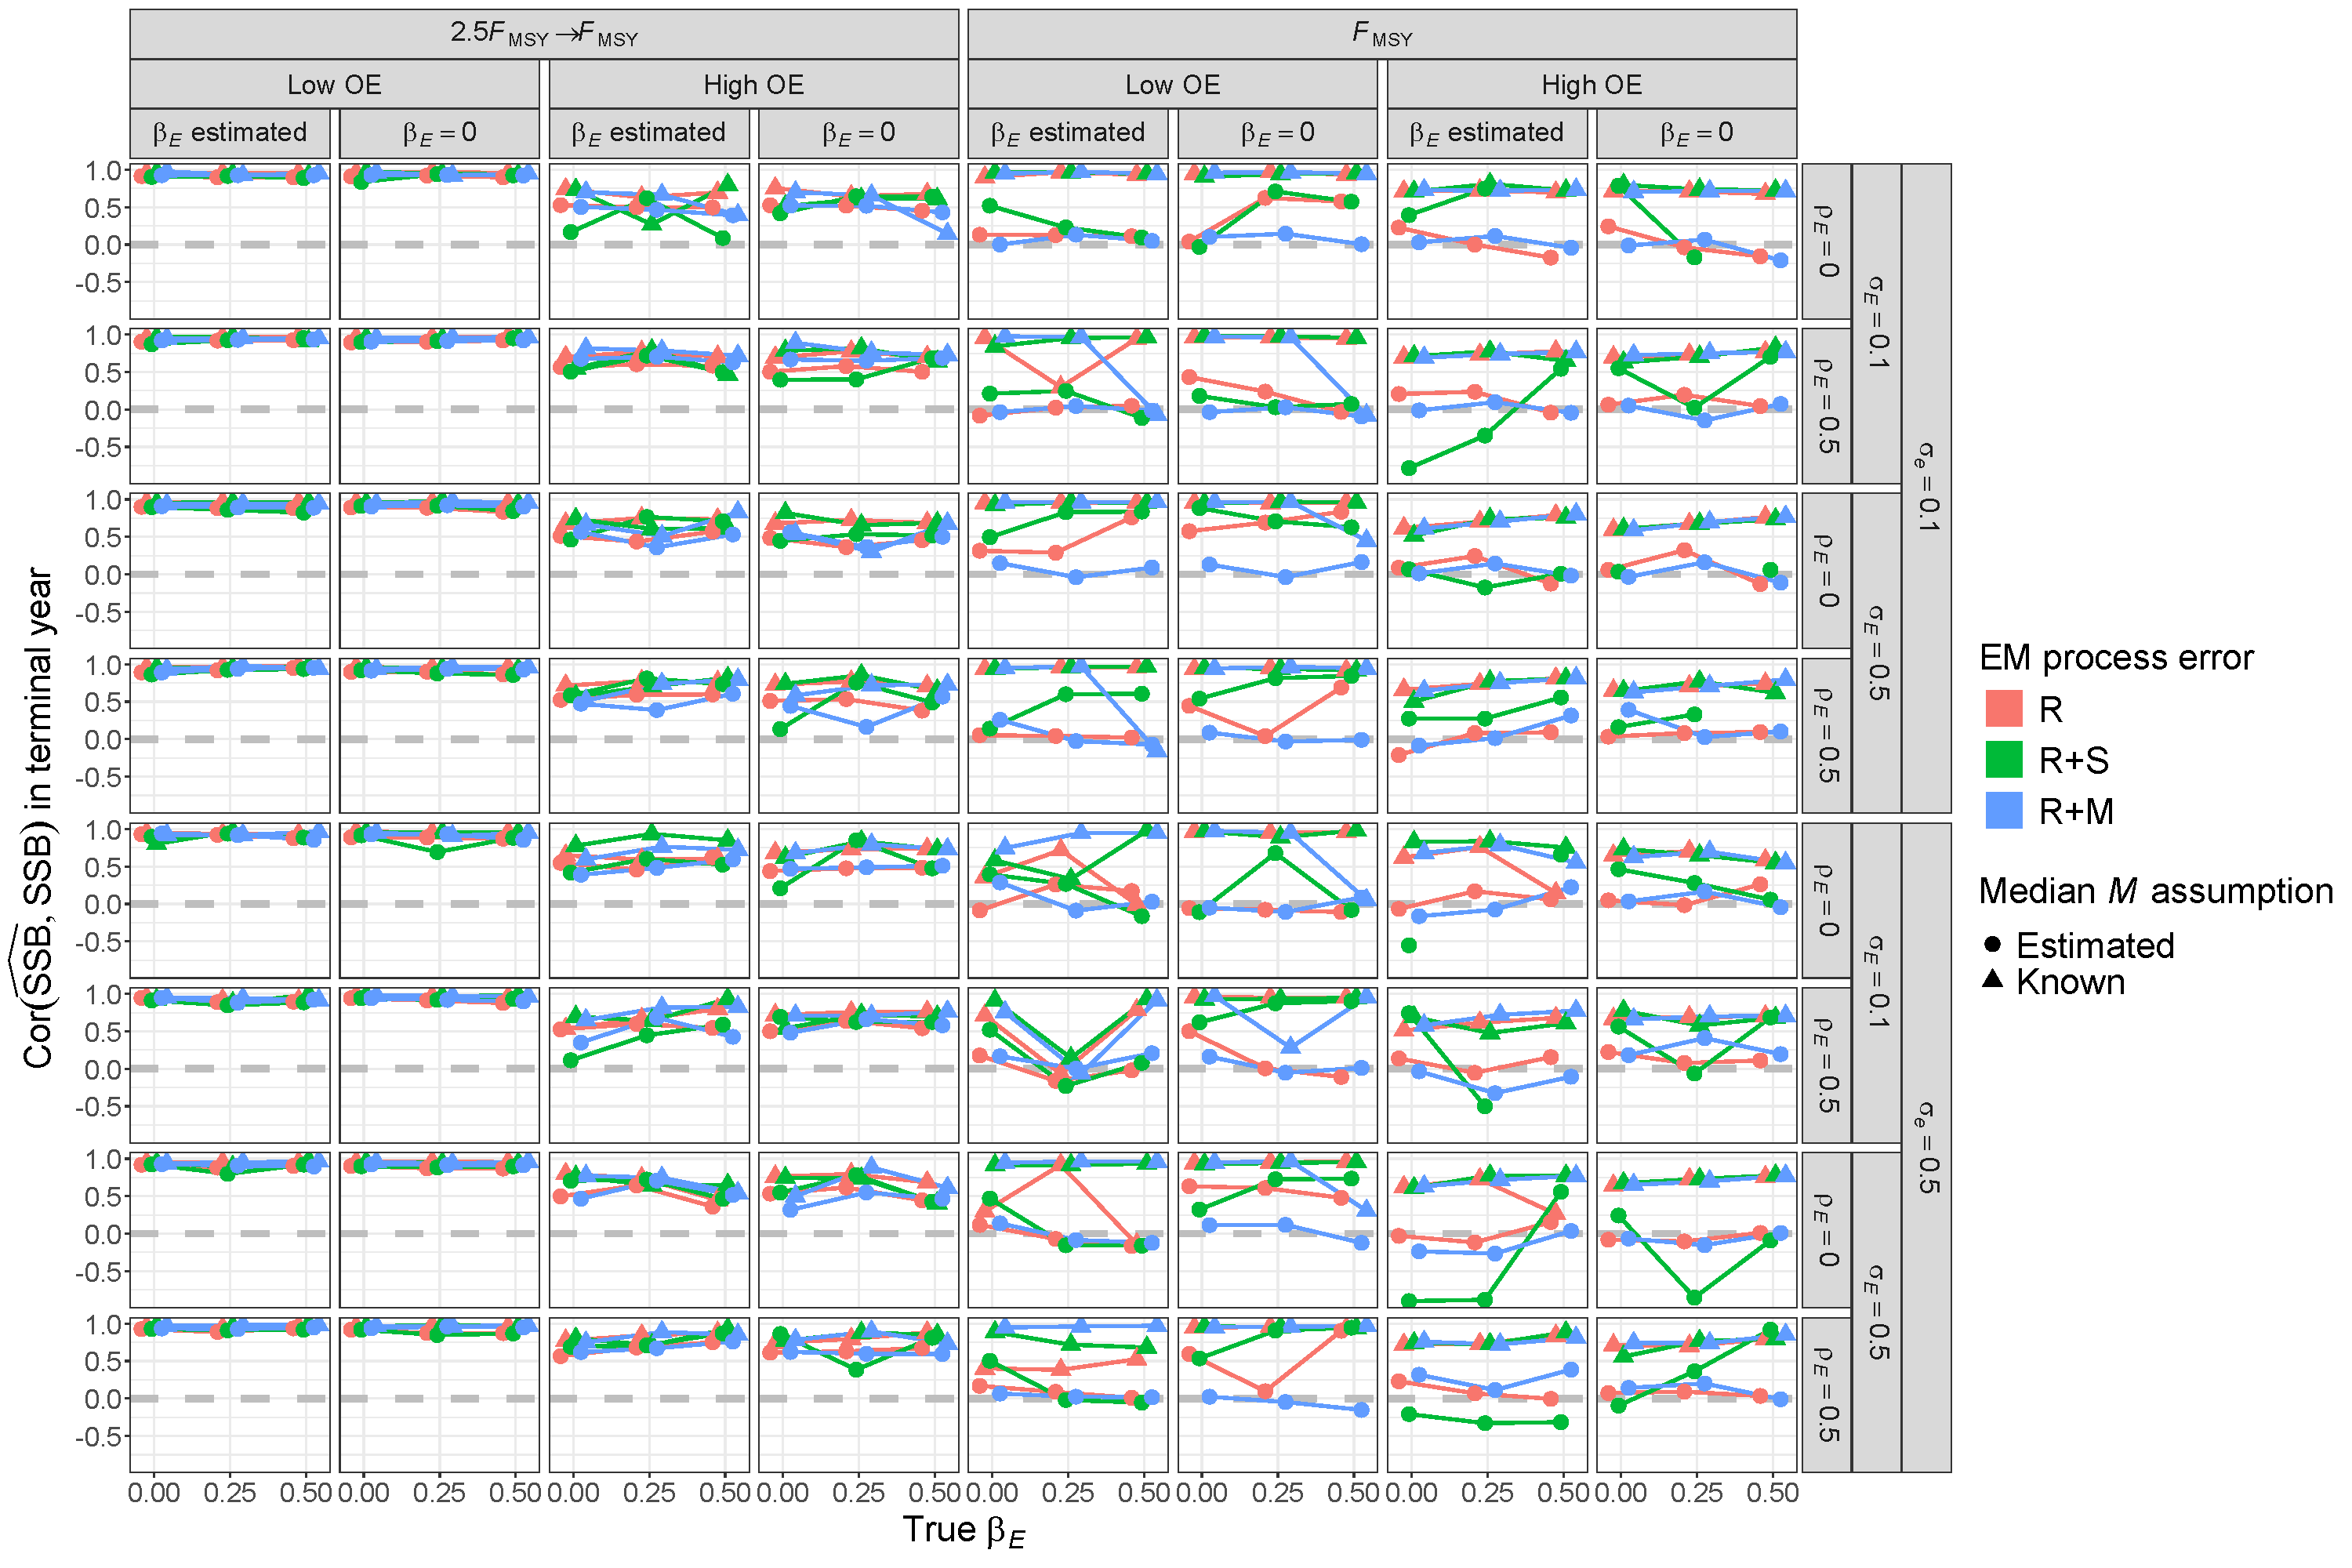
\includegraphics[height = \textheight]{terminal_year_ssb_corr_RMom}
\end{center}
\caption{\DIFaddFL{For R+M OMs, correlation of estimates and true vales of terminal year SSB for EMs with alternative process error assumptions, treatment of covariate effect ($\beta_E = 0$ or estimated), and treatment of median $M$ parameter ($\beta_M$ estimated or known).}}\label{terminal_ssb_corr_RMom}
\end{figure}
\end{landscape}

\subsection*{\DIFadd{Terminal year fishing mortality bias}}\label{terminal-year-fishing-mortality-bias}
\DIFaddend \addcontentsline{toc}{subsection}{Terminal year fishing mortality bias}

\begin{landscape}
\begin{figure}
\begin{center}
\DIFdelbeginFL %DIFDELCMD < 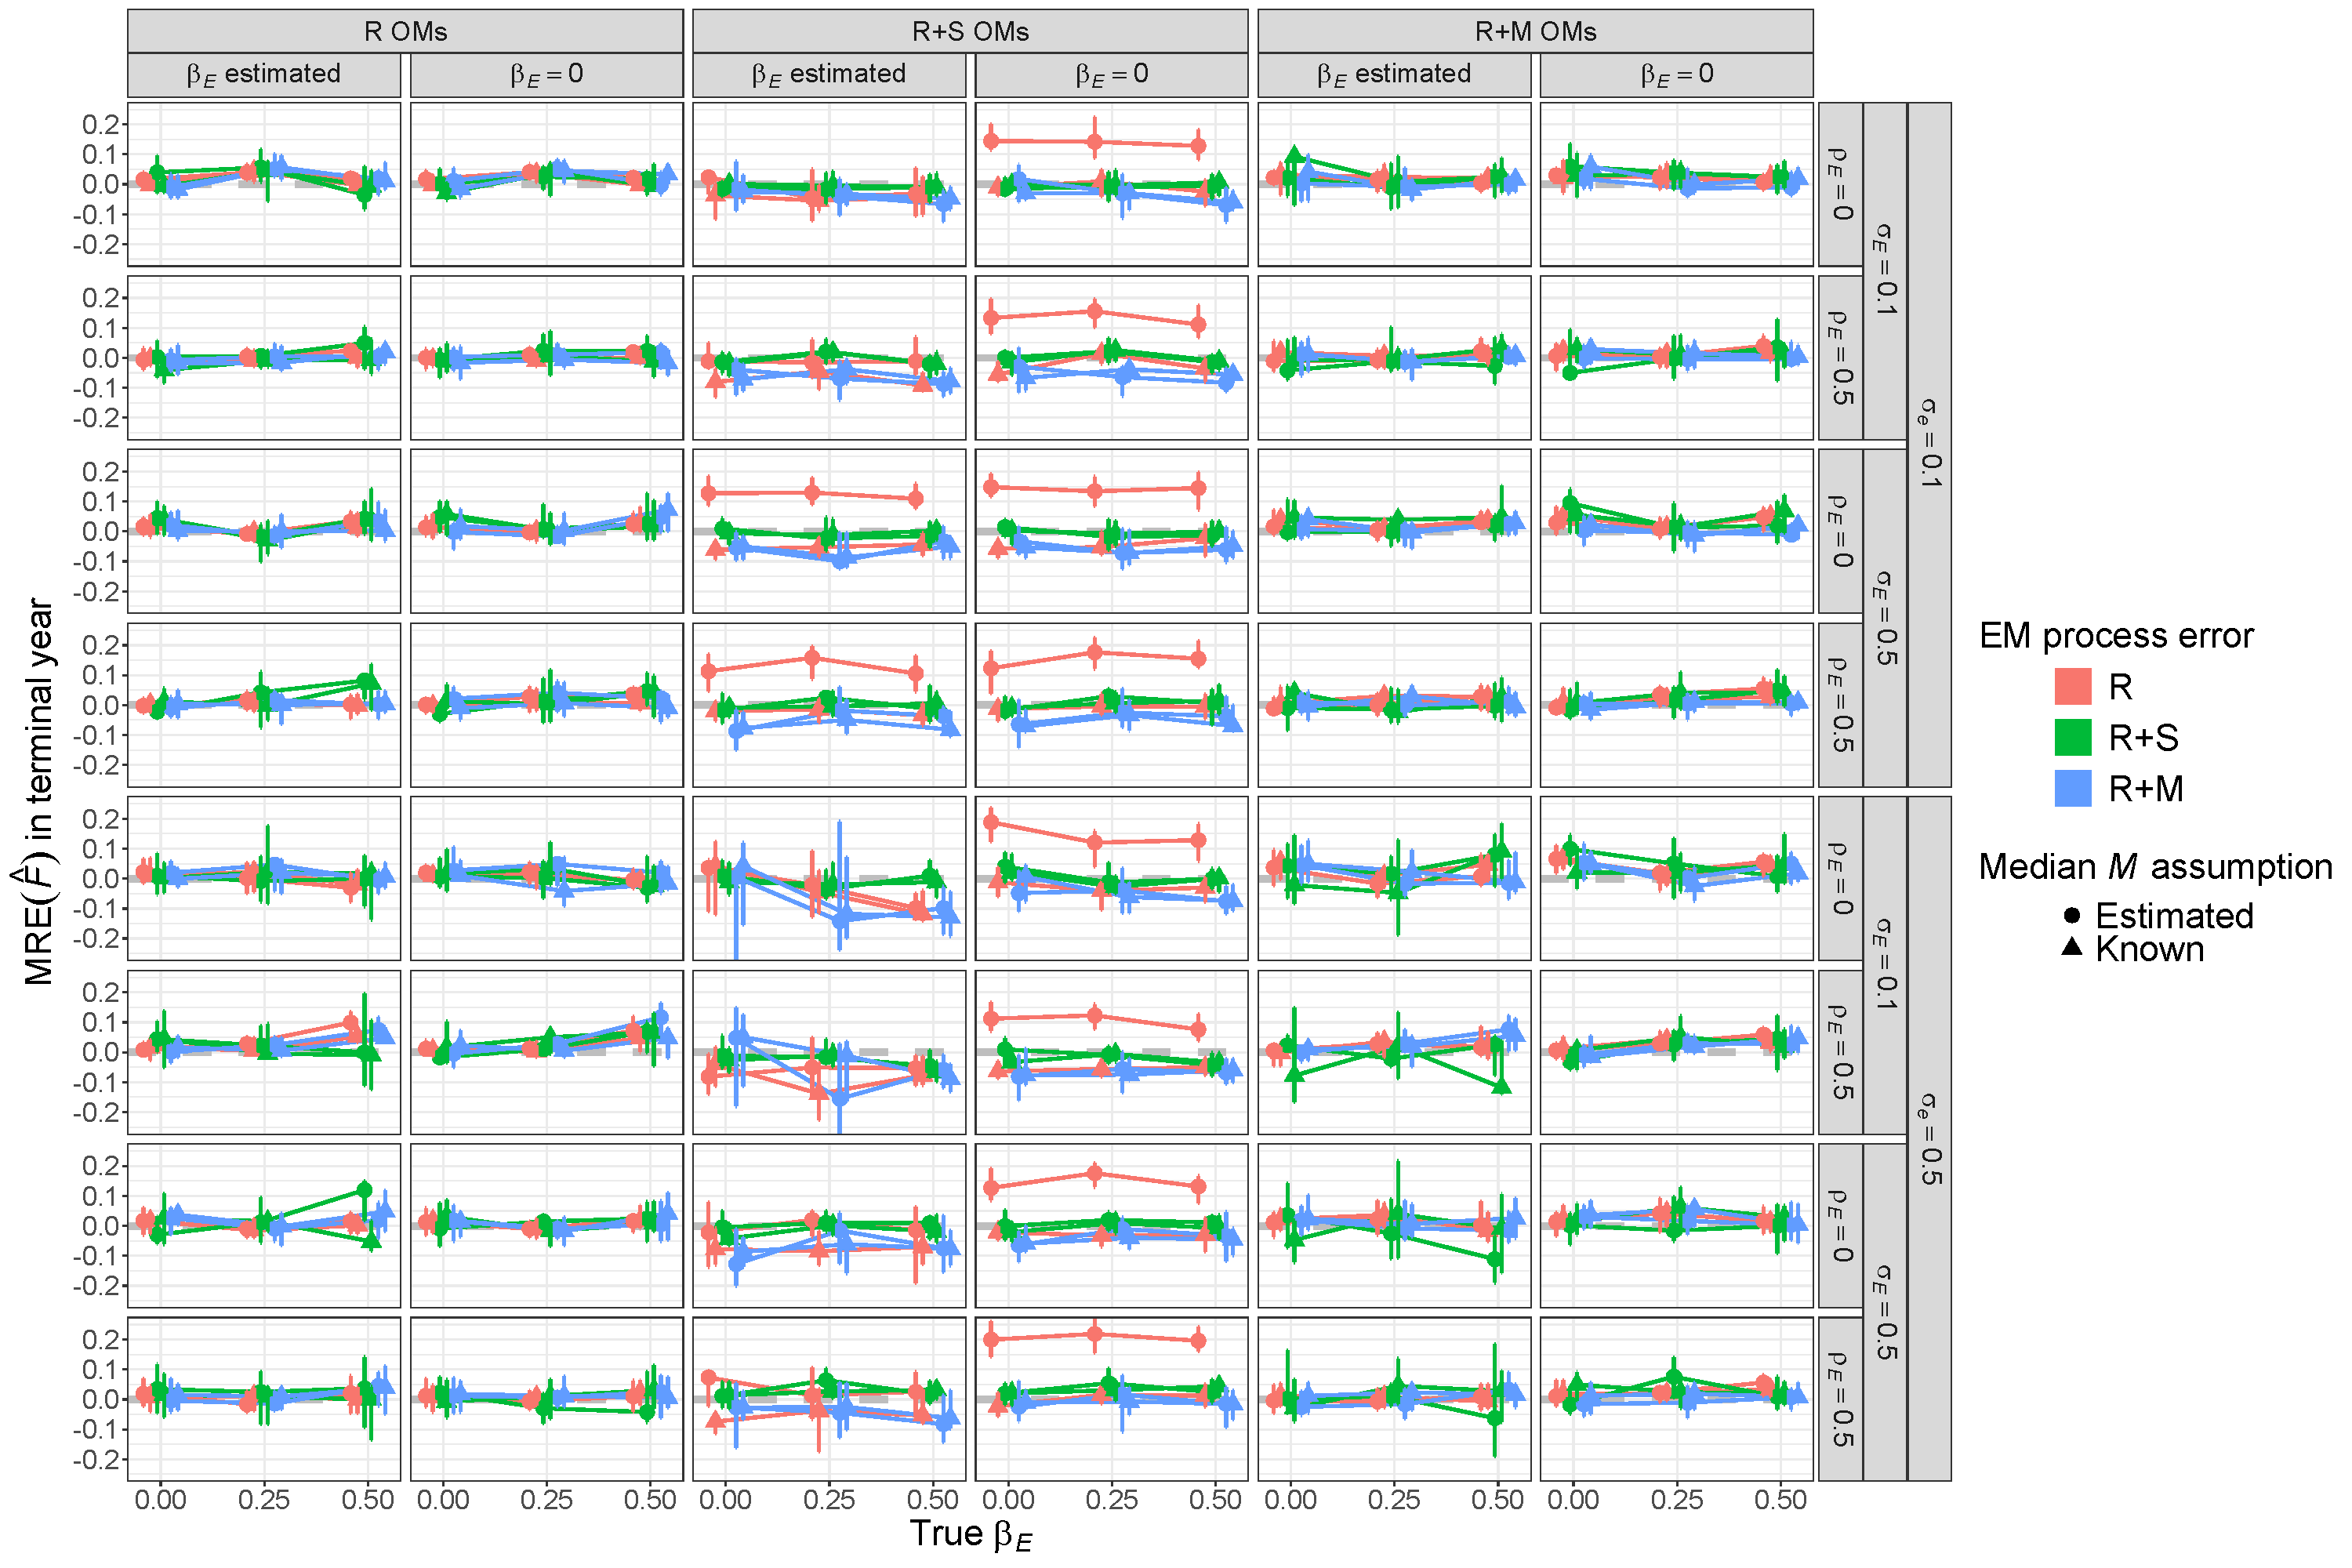
\includegraphics[height = \textheight]{terminal_year_F_bias_main}
%DIFDELCMD < %%%
\DIFdelendFL \DIFaddbeginFL 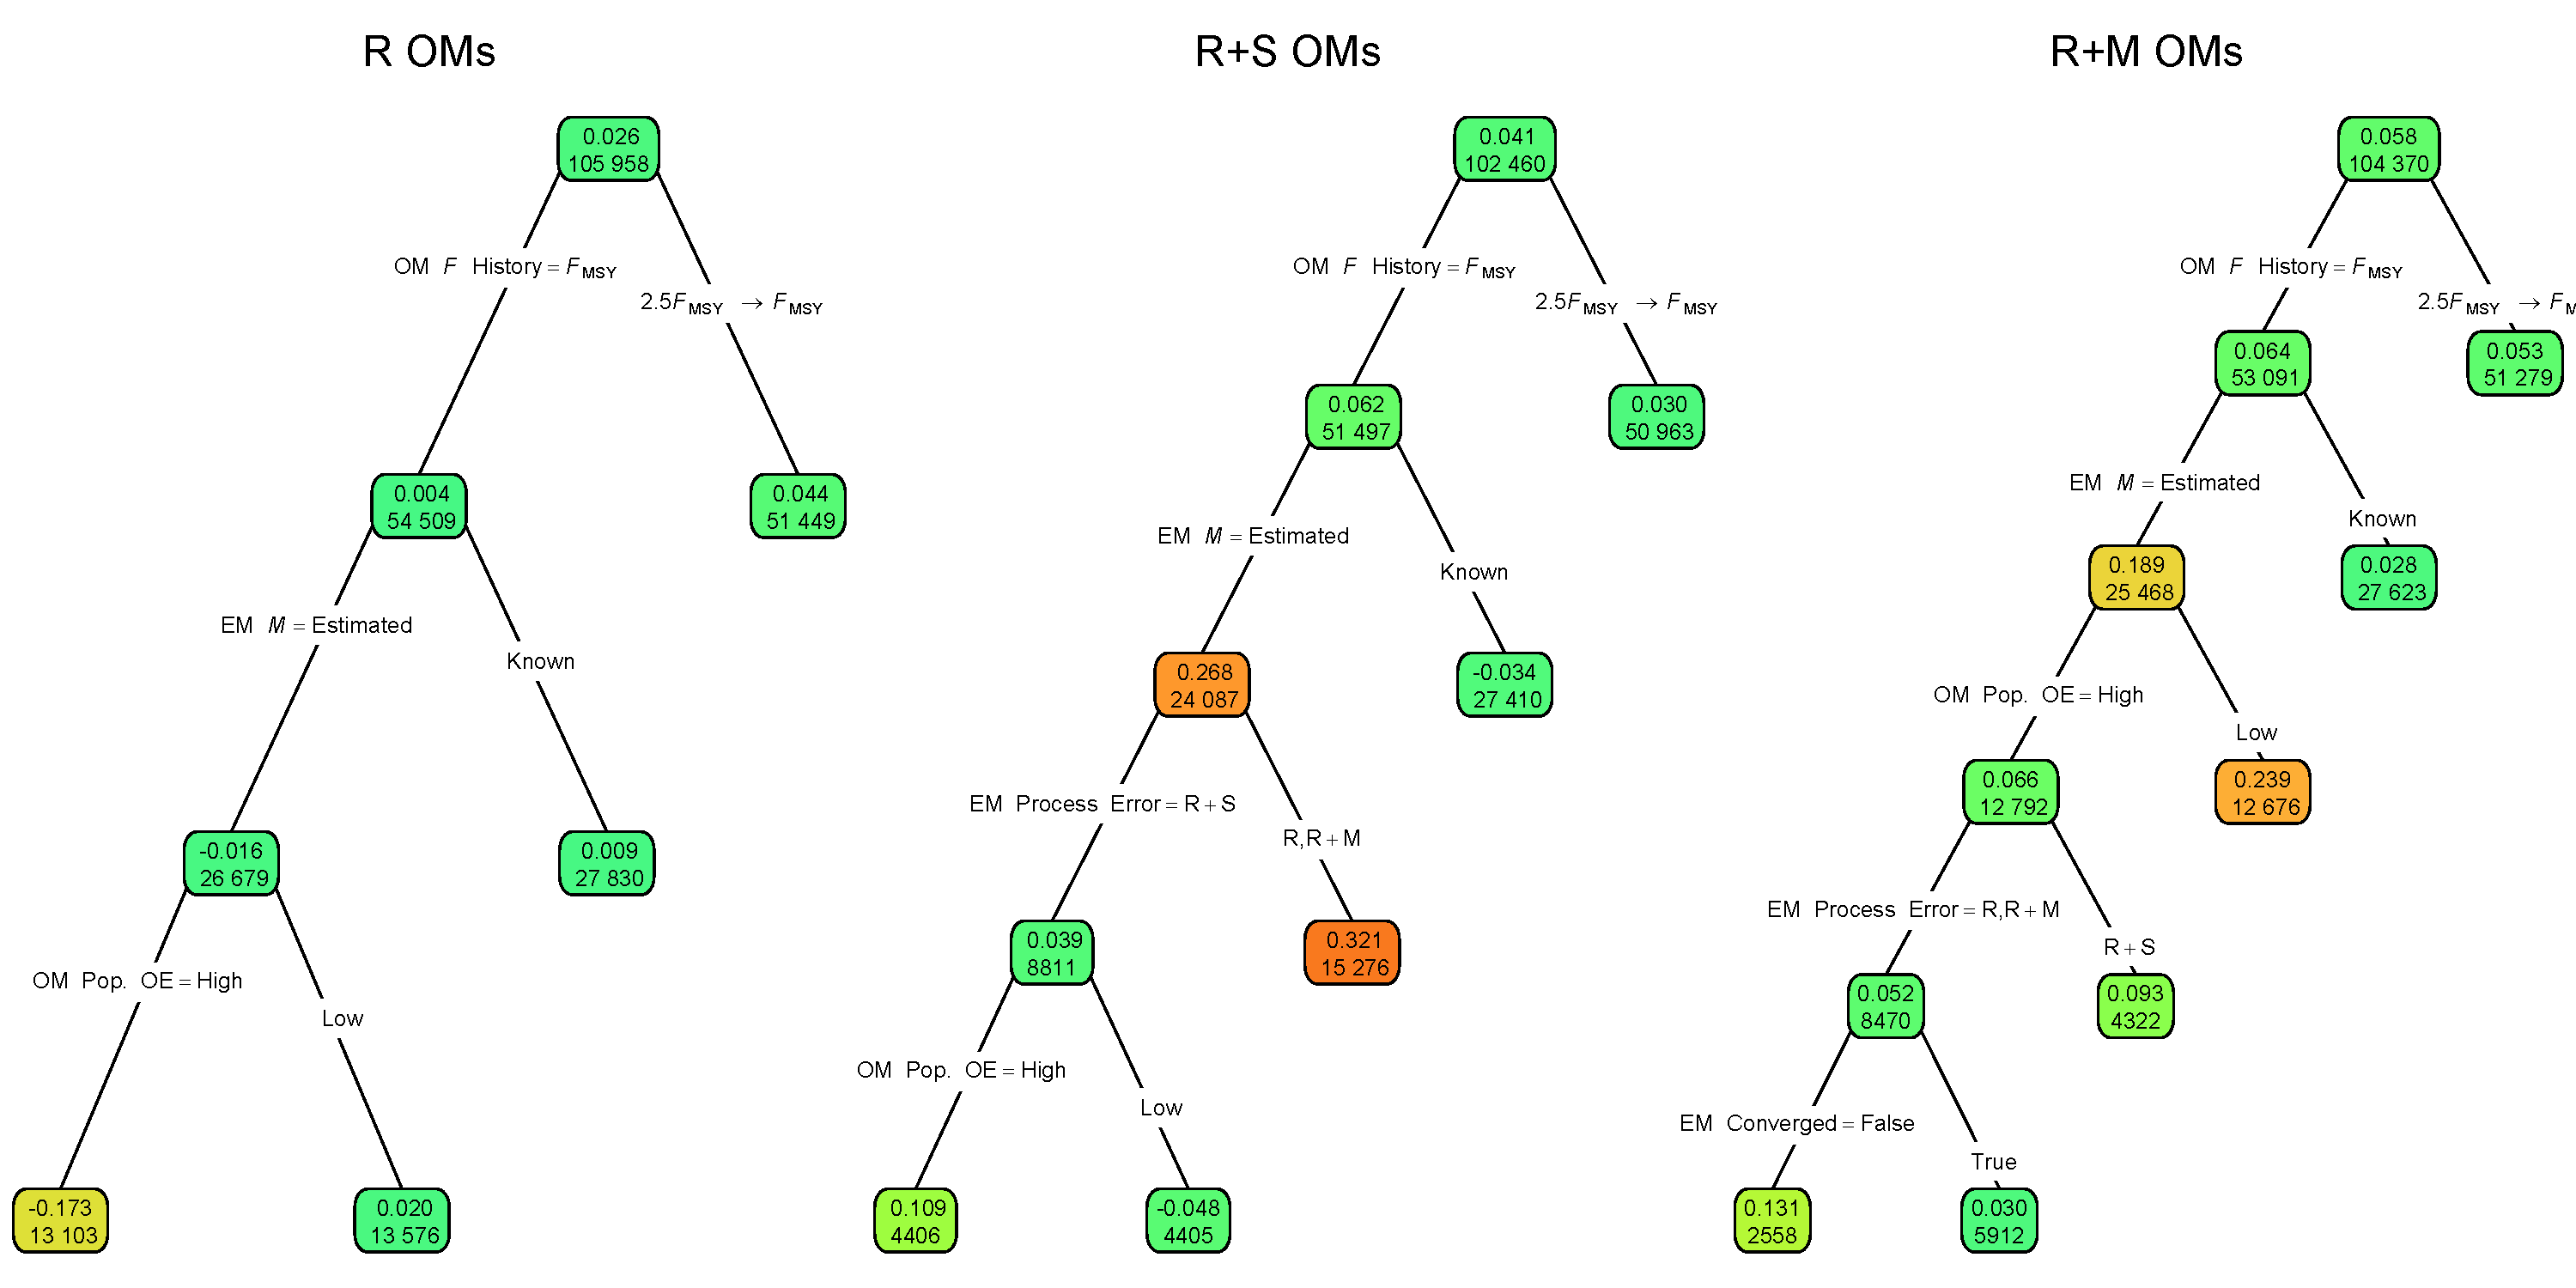
\includegraphics[width = 1.4\textwidth]{term_F_bias_regtree_plots}
\DIFaddendFL \end{center}
\caption{\DIFdelbeginFL \DIFdelFL{Median relative error (MRE) }\DIFdelendFL \DIFaddbeginFL \DIFaddFL{Regression trees indicating primary factors determining reductions in sums }\DIFaddendFL of \DIFdelbeginFL \DIFdelFL{estimates }\DIFdelendFL \DIFaddbeginFL \DIFaddFL{squares }\DIFaddendFL of \DIFdelbeginFL \DIFdelFL{fully-selected fishing mortality ($F$) }\DIFdelendFL \DIFaddbeginFL \DIFaddFL{errors }\DIFaddendFL in \DIFaddbeginFL \DIFaddFL{estimation measured by Eq. \ref{relerror_trans_response} for }\DIFaddendFL the terminal year \DIFdelbeginFL \DIFdelFL{for }\DIFdelendFL \DIFaddbeginFL \DIFaddFL{fishing mortality rate in }\DIFaddendFL EMs \DIFaddbeginFL \DIFaddFL{fitted to operating models (OMs) }\DIFaddendFL with \DIFdelbeginFL \DIFdelFL{alternative }\DIFdelendFL process error \DIFdelbeginFL \DIFdelFL{assumptions}\DIFdelendFL \DIFaddbeginFL \DIFaddFL{on recruitment only (R)}\DIFaddendFL , \DIFdelbeginFL \DIFdelFL{treatment of covariate effect }\DIFdelendFL \DIFaddbeginFL \DIFaddFL{recruitment and apparent survival }\DIFaddendFL (\DIFdelbeginFL \DIFdelFL{$\beta_E = 0$ or estimated}\DIFdelendFL \DIFaddbeginFL \DIFaddFL{R+S}\DIFaddendFL ), \DIFaddbeginFL \DIFaddFL{or recruitment }\DIFaddendFL and \DIFdelbeginFL \DIFdelFL{treatment of median }\DIFdelendFL natural mortality \DIFdelbeginFL \DIFdelFL{parameter }\DIFdelendFL (\DIFdelbeginFL \DIFdelFL{$\beta_M$ estimated or known}\DIFdelendFL \DIFaddbeginFL \DIFaddFL{R+M}\DIFaddendFL ). \DIFdelbeginFL \DIFdelFL{All OMs had low population observation }\DIFdelendFL \DIFaddbeginFL \DIFaddFL{Each node shows the median }\DIFaddendFL error \DIFaddbeginFL \DIFaddFL{(top) }\DIFaddendFL and \DIFdelbeginFL \DIFdelFL{contrast in fishing mortality}\DIFdelendFL \DIFaddbeginFL \DIFaddFL{number of observations (bottom) for the corresponding subset}\DIFaddendFL . \DIFaddbeginFL \DIFaddFL{Lower or higher median absolute errors of the process error assumption are indicated by more green or red polygons, respectively.}\DIFaddendFL }\DIFdelbeginFL %DIFDELCMD < \label{terminal_F_bias}
%DIFDELCMD < %%%
\DIFdelendFL \DIFaddbeginFL \label{term_F_bias_regtree}
\DIFaddendFL \end{figure}
\end{landscape}

\begin{landscape}
\begin{figure}
\begin{center}
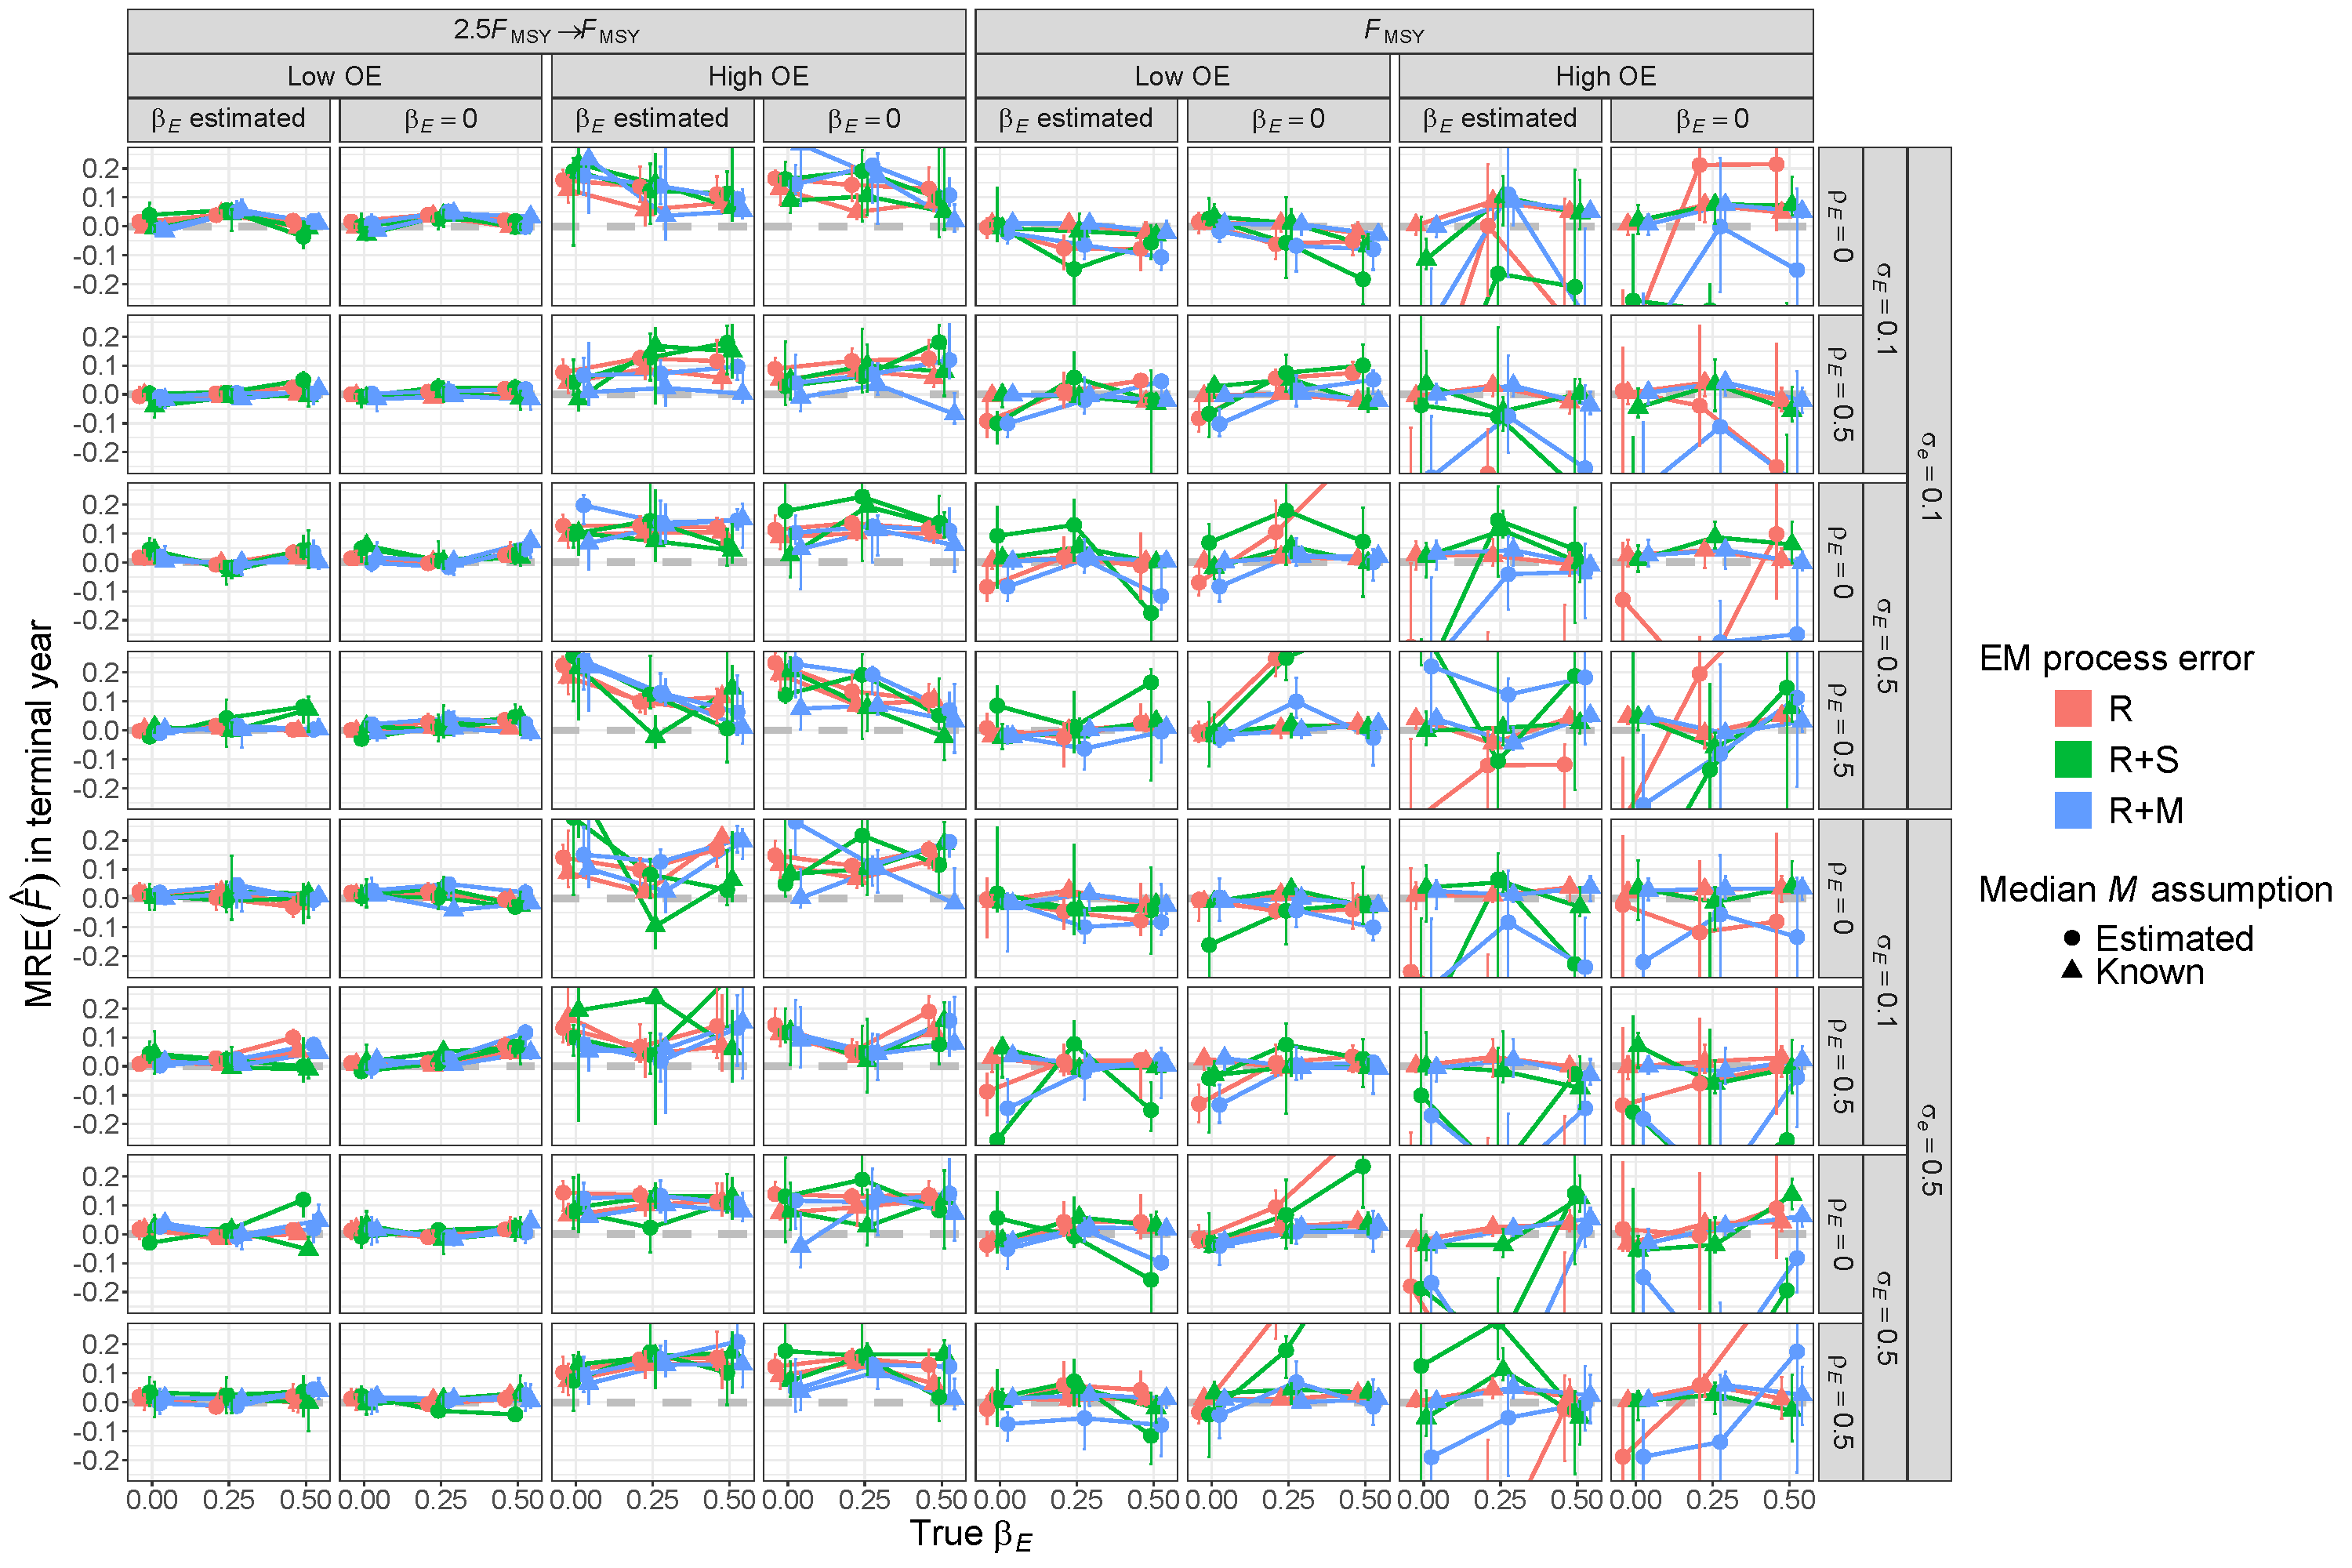
\includegraphics[height = \textheight]{terminal_year_F_bias_Rom}
\end{center}
\caption{For R OMs, median relative error (MRE) of estimates of fully-selected fishing mortality ($F$) in the terminal year for EMs with alternative process error assumptions, treatment of covariate effect ($\beta_E = 0$ or estimated), and treatment of median \DIFdelbeginFL \DIFdelFL{natural mortality }\DIFdelendFL \DIFaddbeginFL \DIFaddFL{$M$ }\DIFaddendFL parameter ($\beta_M$ estimated or known). All OMs had low observation error and contrast in fishing mortality.}\label{terminal_F_bias_Rom}
\end{figure}
\end{landscape}

\begin{landscape}
\begin{figure}
\begin{center}
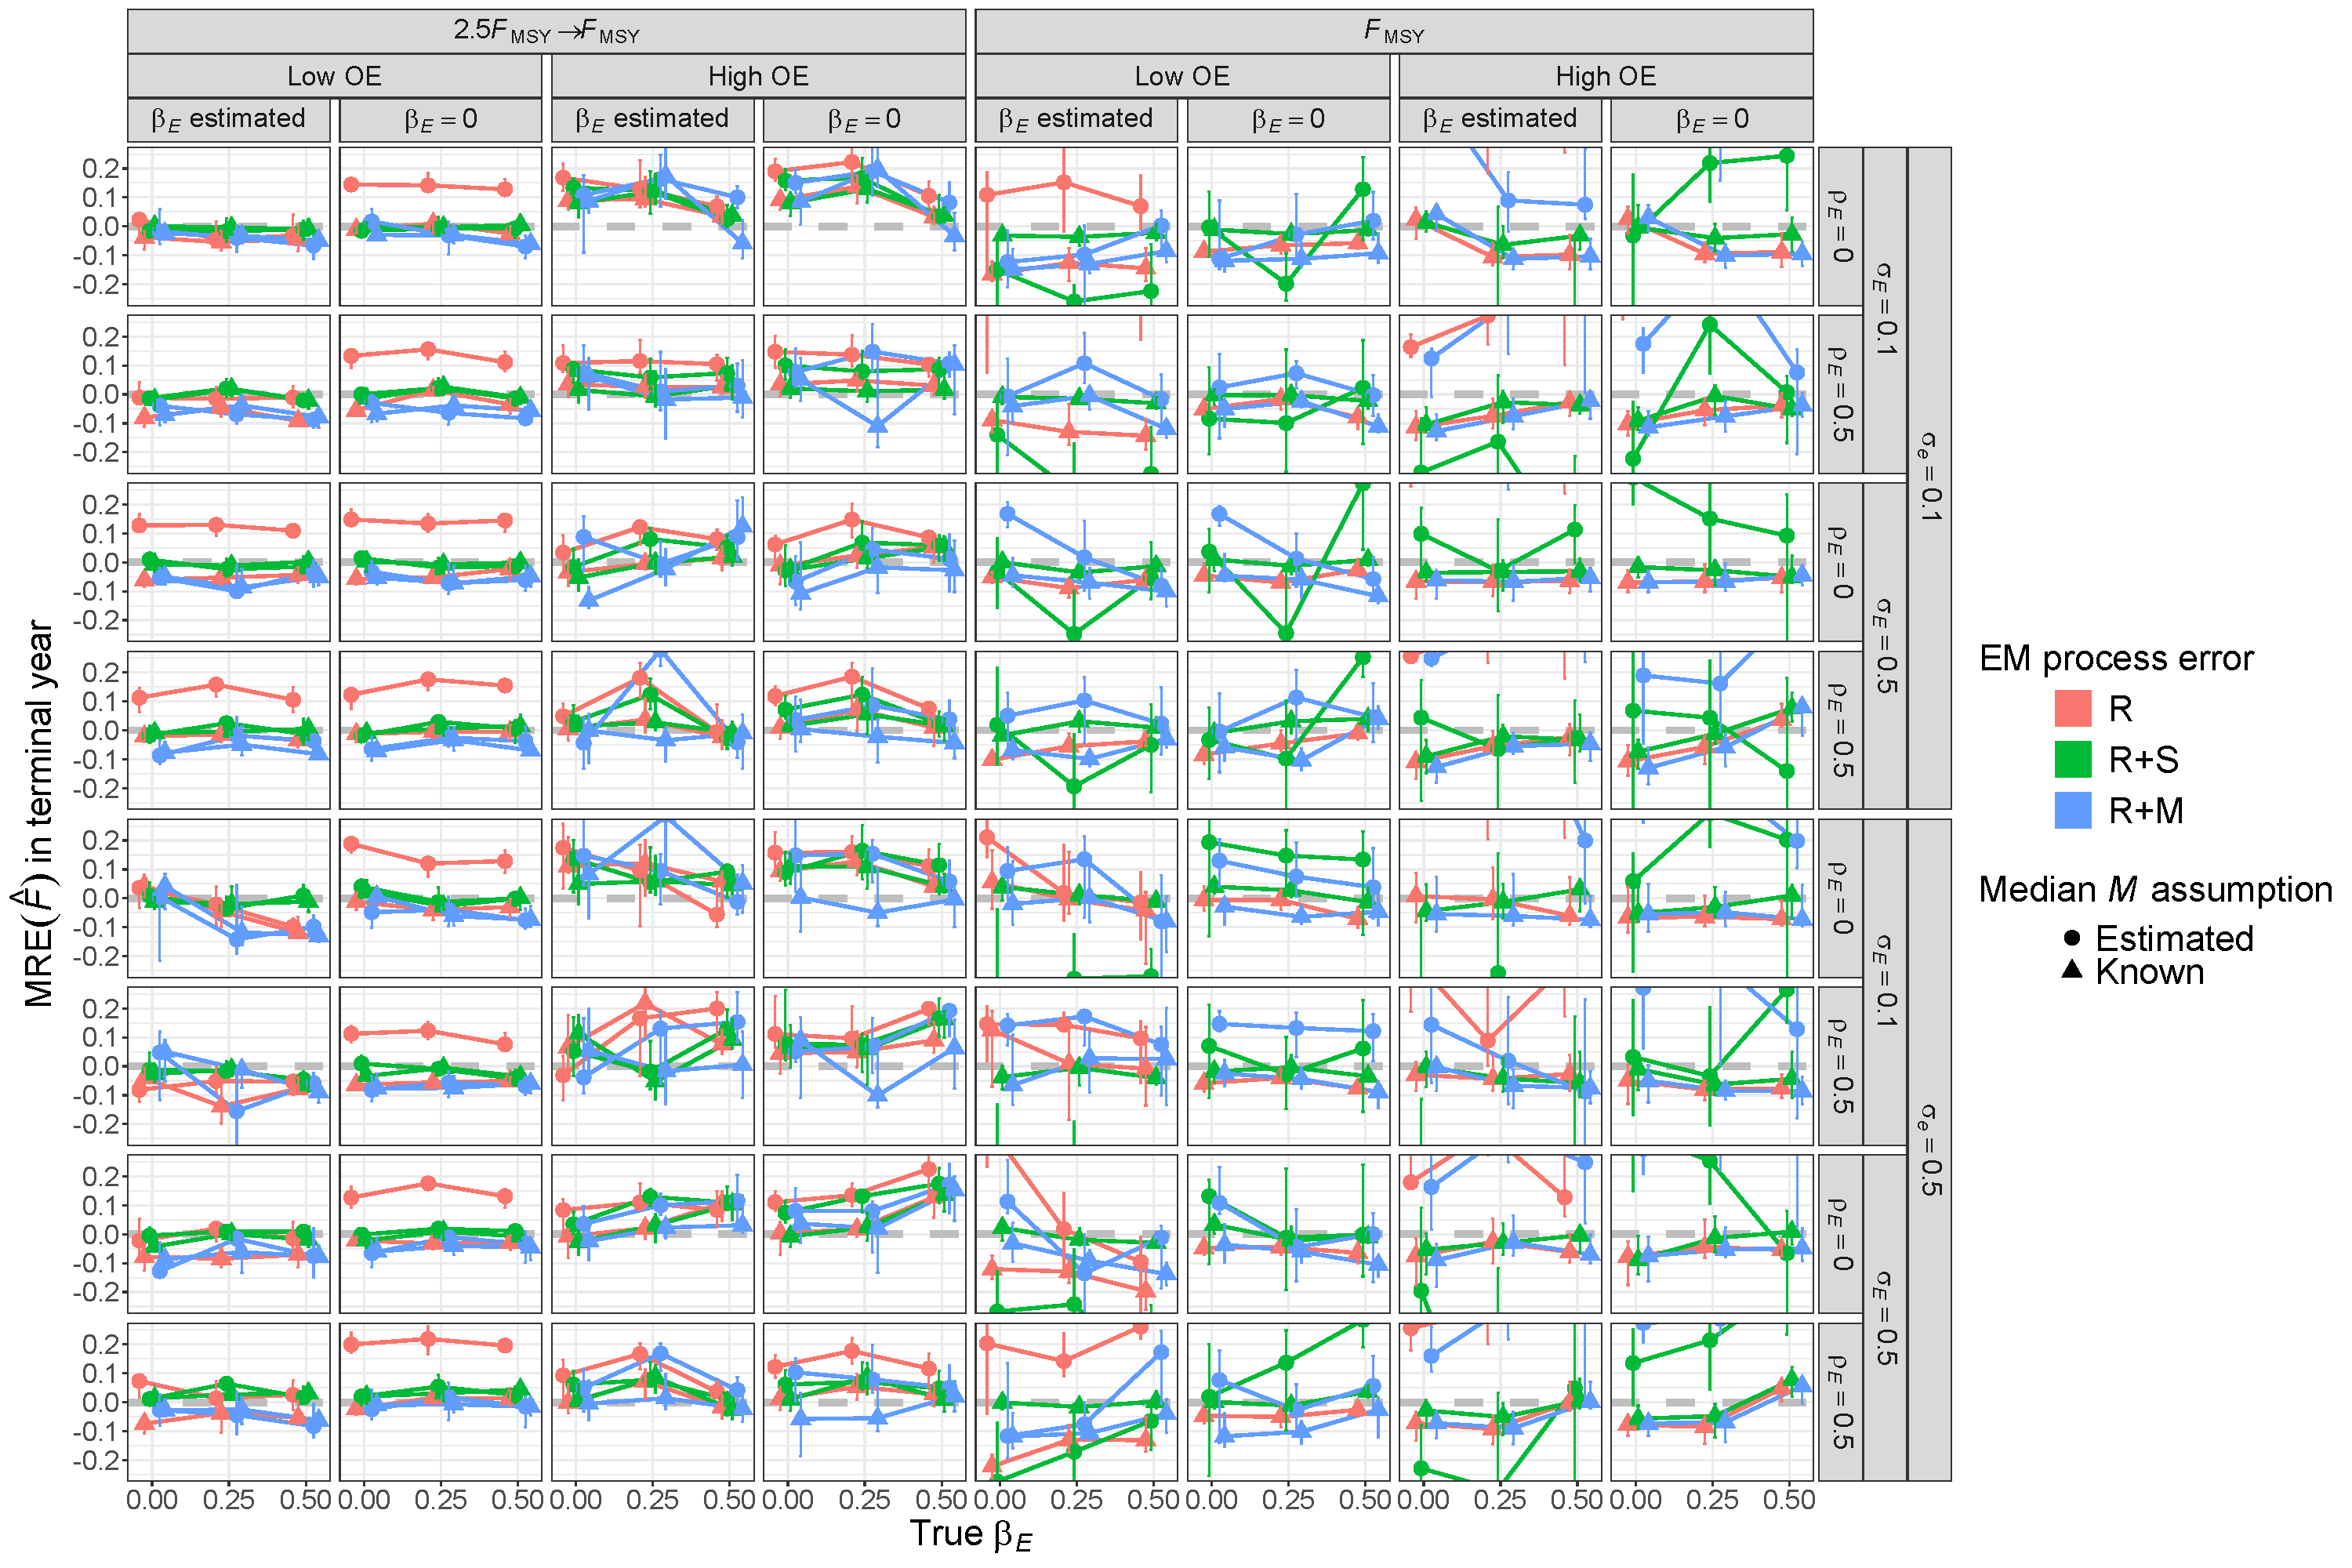
\includegraphics[height = \textheight]{terminal_year_F_bias_RSom}
\end{center}
\caption{For R+S OMs, median relative error (MRE) of estimates of fully-selected fishing mortality ($F$) in the terminal year for EMs with alternative process error assumptions, treatment of covariate effect ($\beta_E = 0$ or estimated), and treatment of median \DIFdelbeginFL \DIFdelFL{natural mortality }\DIFdelendFL \DIFaddbeginFL \DIFaddFL{$M$ }\DIFaddendFL parameter ($\beta_M$ estimated or known). All OMs had low observation error and contrast in fishing mortality.}\label{terminal_F_bias_RSom}
\end{figure}
\end{landscape}

\begin{landscape}
\begin{figure}
\begin{center}
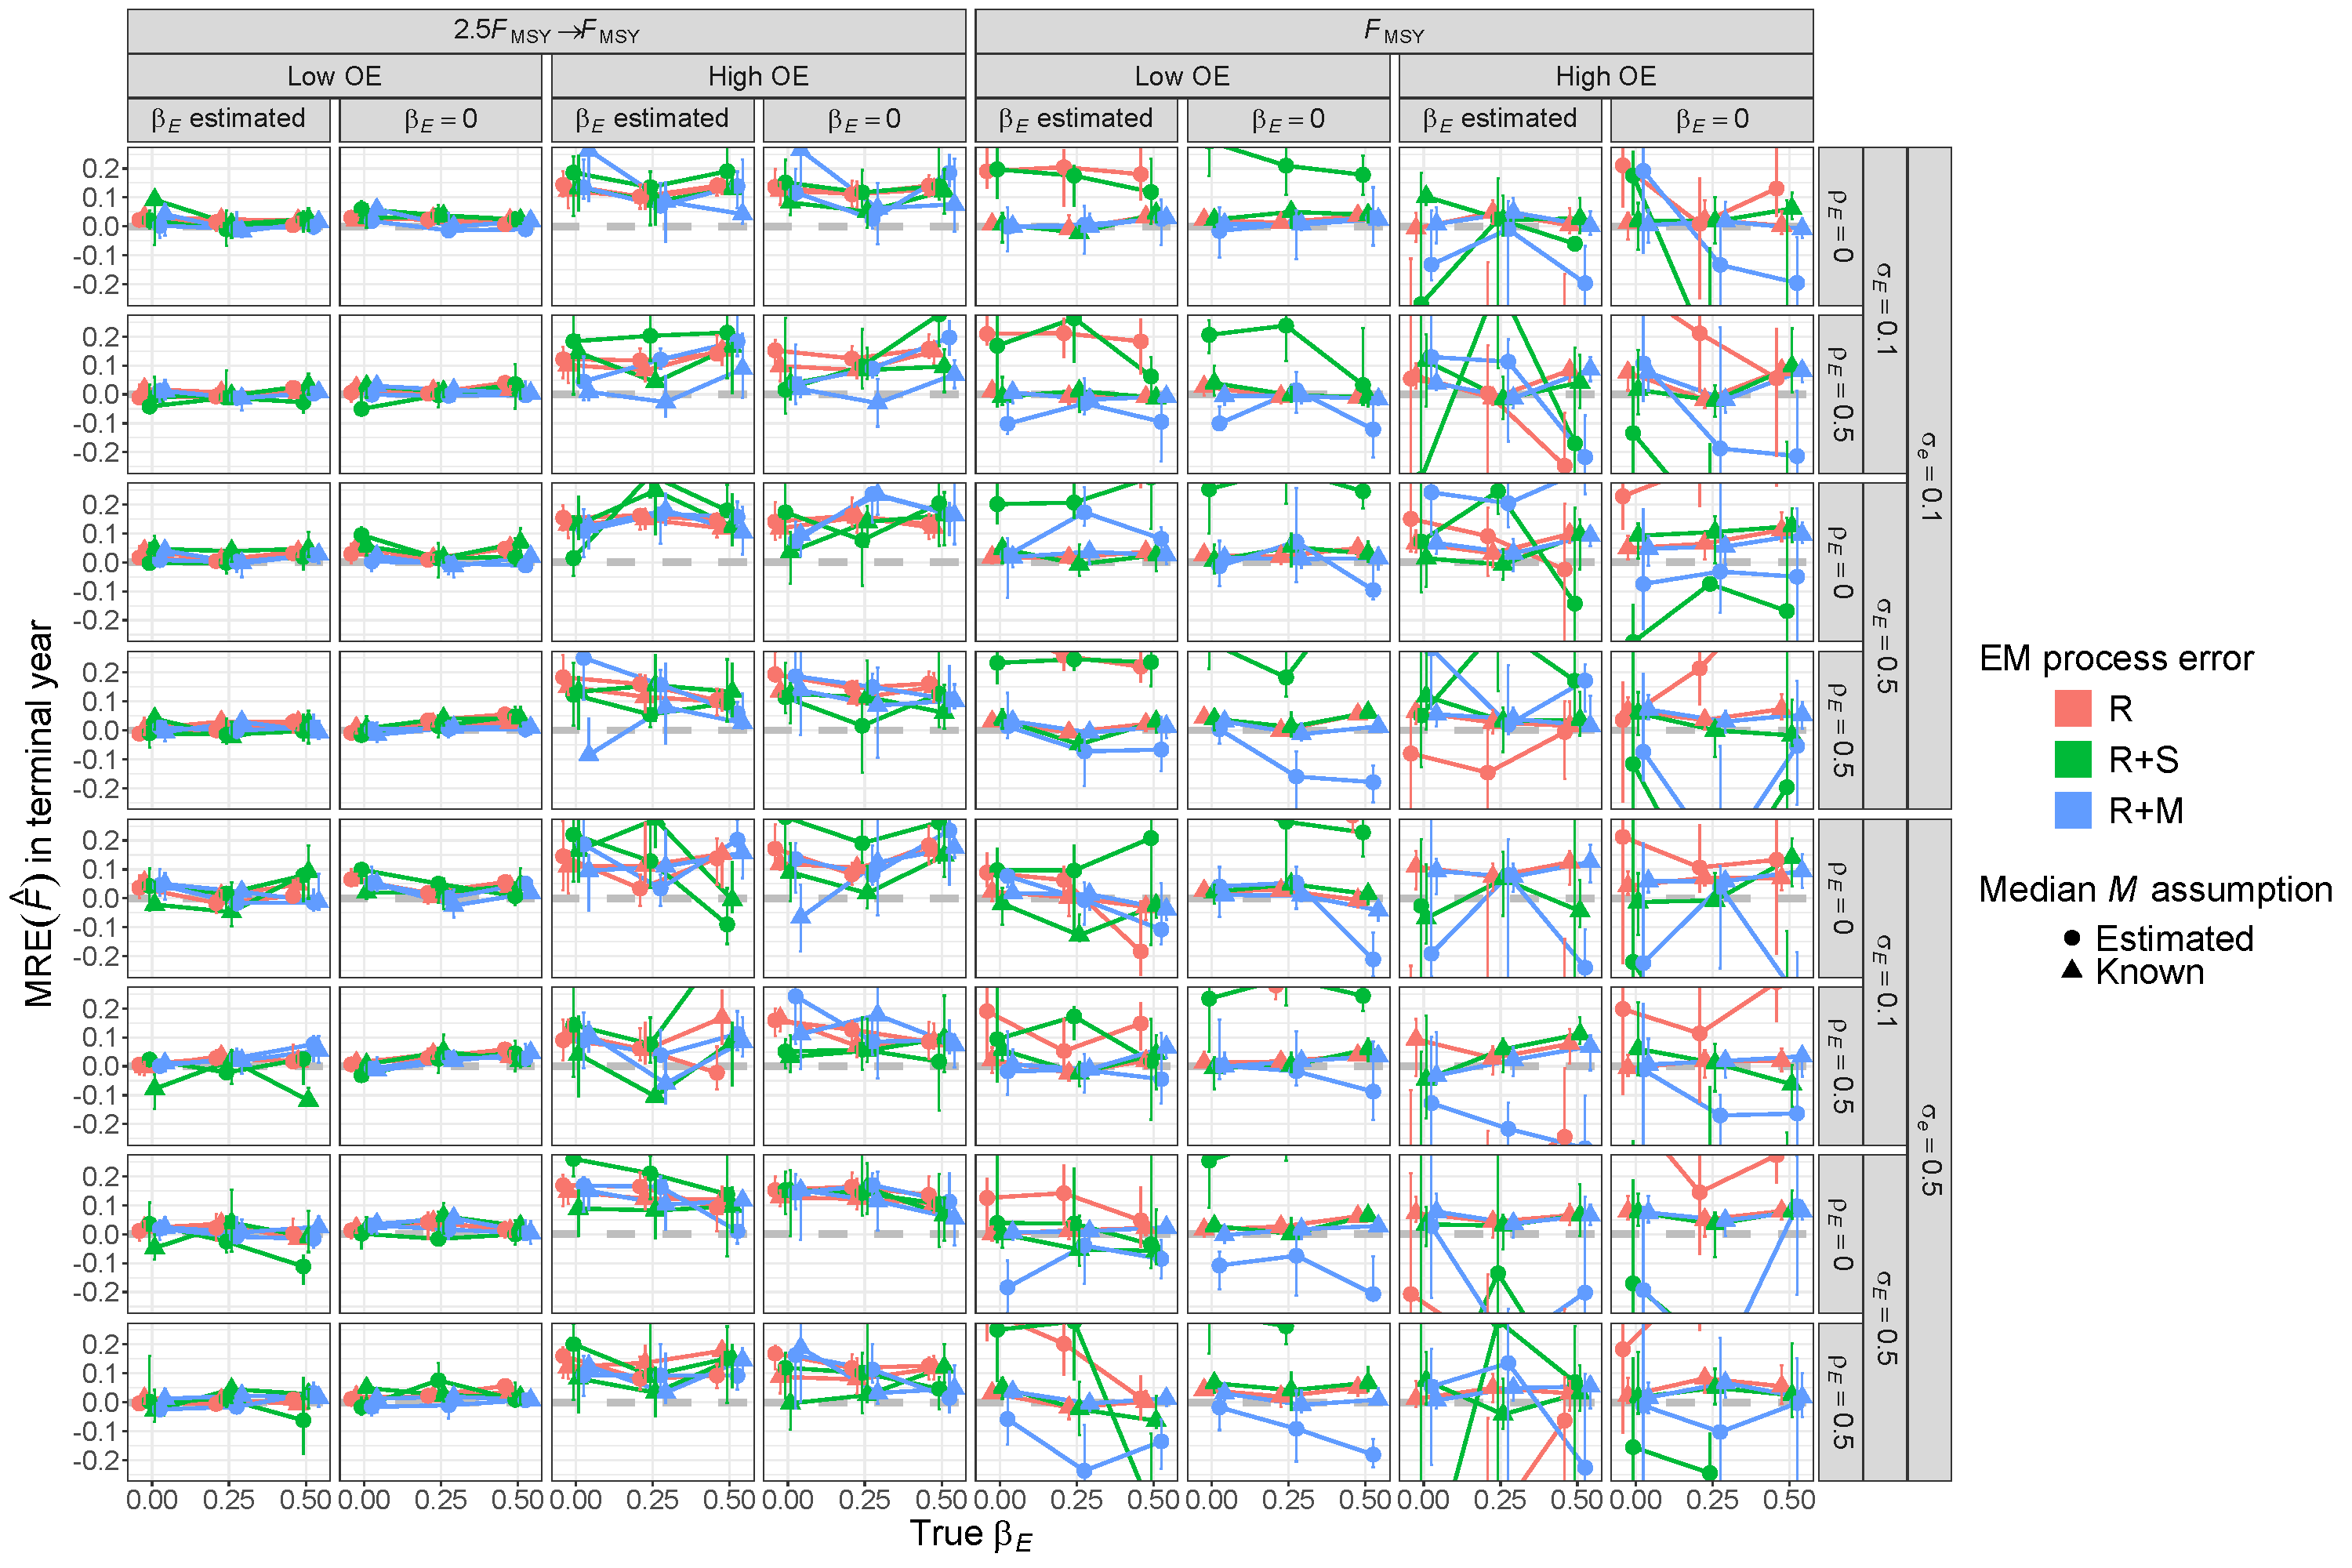
\includegraphics[height = \textheight]{terminal_year_F_bias_RMom}
\end{center}
\caption{For R+M OMs, median relative error (MRE) of estimates of fully-selected fishing mortality ($F$) in the terminal year for EMs with alternative process error assumptions, treatment of covariate effect ($\beta_E = 0$ or estimated), and treatment of median \DIFdelbeginFL \DIFdelFL{natural mortality }\DIFdelendFL \DIFaddbeginFL \DIFaddFL{$M$ }\DIFaddendFL parameter ($\beta_M$ estimated or known). All OMs had low observation error and contrast in fishing mortality.}\label{terminal_F_bias_RMom}
\end{figure}
\end{landscape}

\DIFdelbegin %DIFDELCMD < \hypertarget{terminal-year-fishing-mortality-rmse}{%
%DIFDELCMD < \subsection*{Terminal year fishing mortality RMSE}\label{terminal-year-fishing-mortality-rmse}}
%DIFDELCMD < %%%
\DIFdelend \DIFaddbegin \subsection*{\DIFadd{Terminal year fishing mortality accuracy}}\label{terminal-year-fishing-mortality-accuracy}
\DIFaddend \addcontentsline{toc}{subsection}{Terminal year fishing mortality \DIFdelbegin \DIFdel{RMSE}\DIFdelend \DIFaddbegin \DIFadd{accuracy}\DIFaddend }

\begin{landscape}
\begin{figure}
\begin{center}
\DIFdelbeginFL %DIFDELCMD < 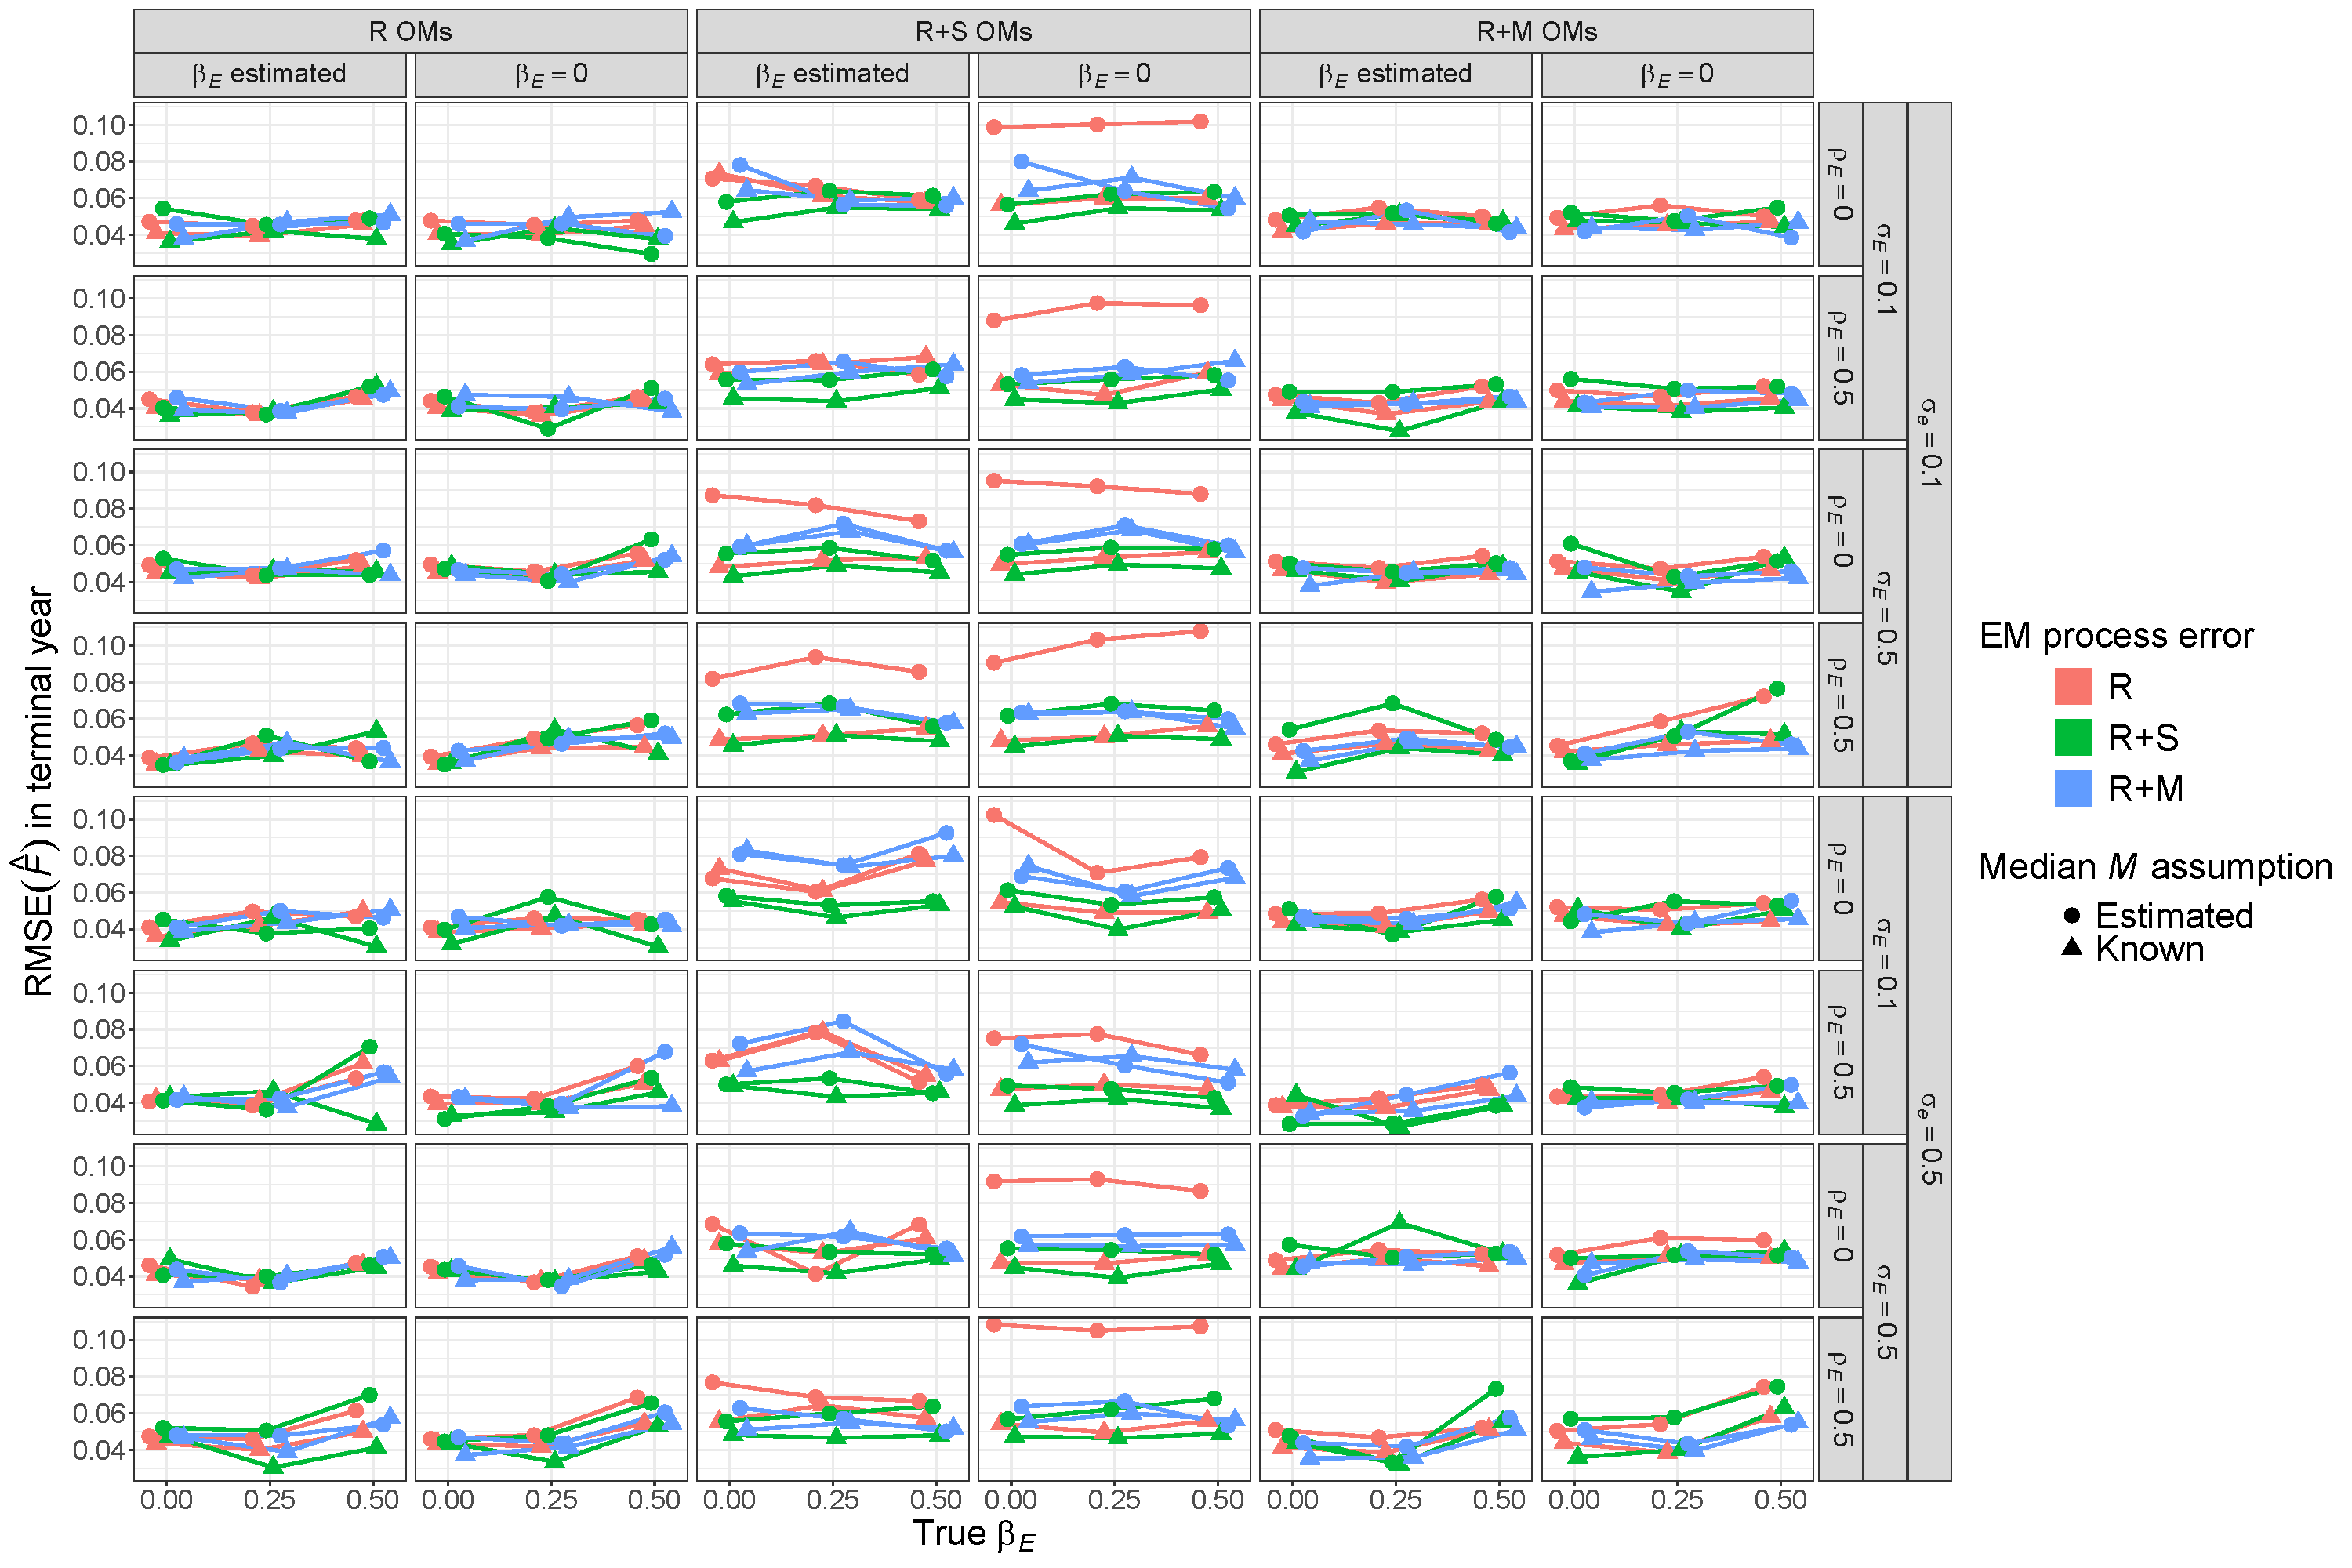
\includegraphics[height = \textheight]{terminal_year_F_rmse_main}
%DIFDELCMD < %%%
\DIFdelendFL \DIFaddbeginFL 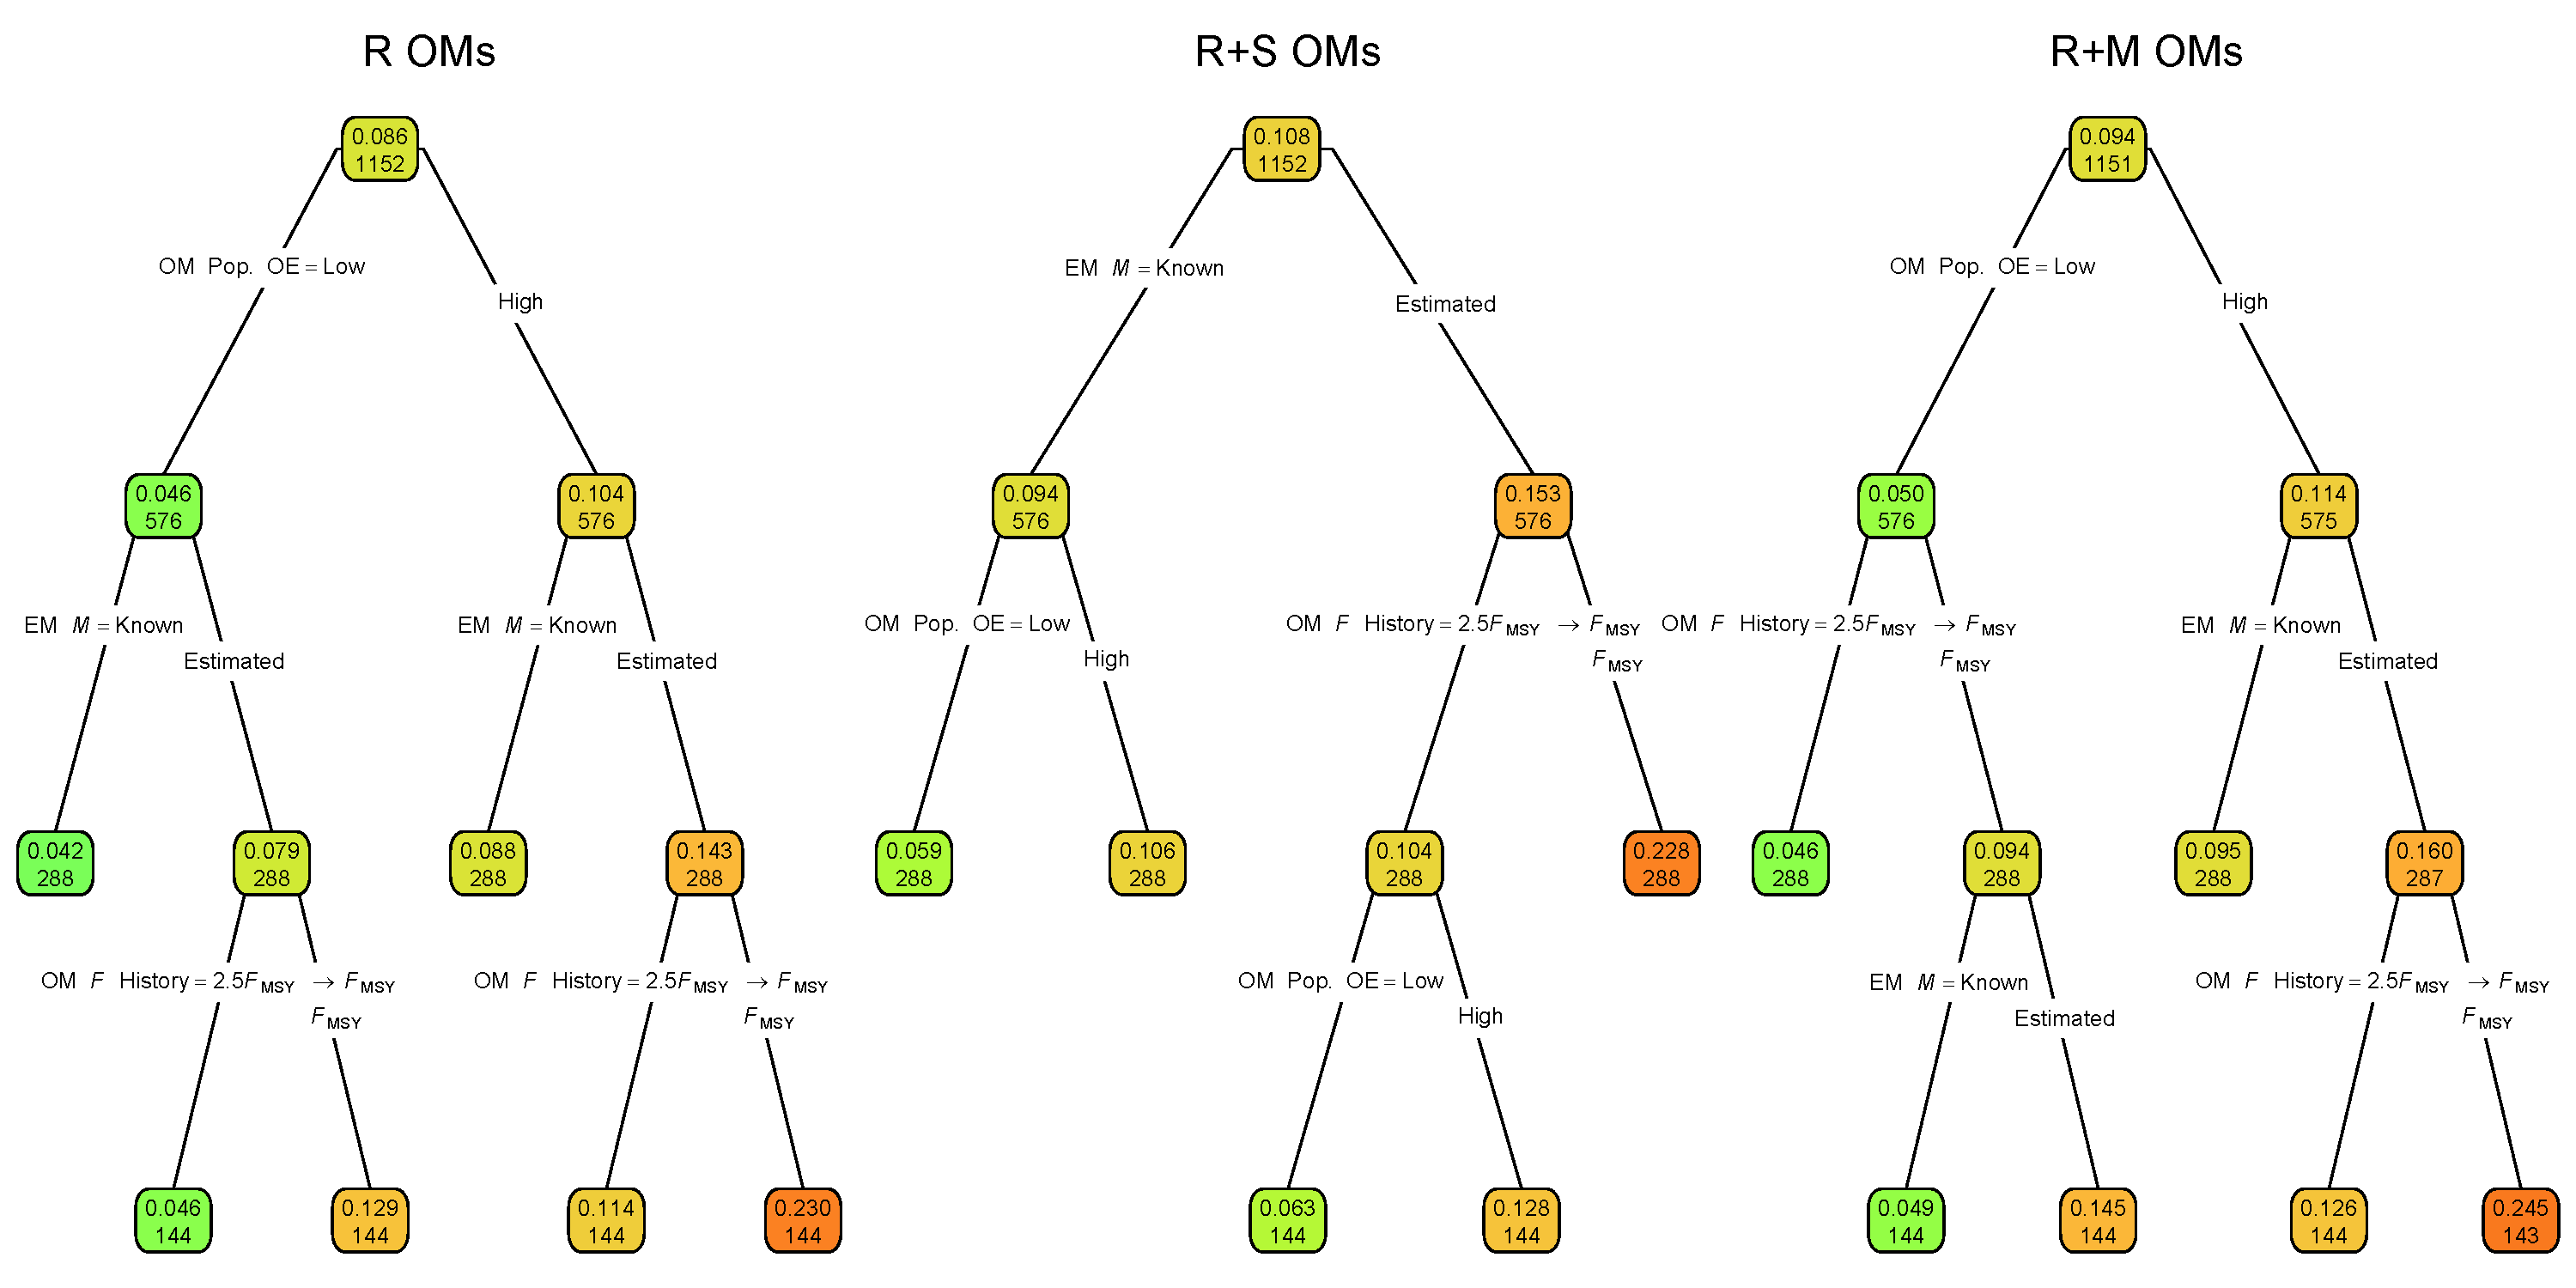
\includegraphics[width = 1.4\textwidth]{term_F_rmse_regtree_plots}
\DIFaddendFL \end{center}
\caption{\DIFdelbeginFL \DIFdelFL{Root mean square error (RMSE) }\DIFdelendFL \DIFaddbeginFL \DIFaddFL{Regression trees indicating primary factors determining reductions in sums }\DIFaddendFL of \DIFdelbeginFL \DIFdelFL{estimates }\DIFdelendFL \DIFaddbeginFL \DIFaddFL{squares }\DIFaddendFL of \DIFdelbeginFL \DIFdelFL{fully-selected fishing mortality ($F$)  in }\DIFdelendFL \DIFaddbeginFL \DIFaddFL{errors for }\DIFaddendFL the \DIFaddbeginFL \DIFaddFL{log-transformed RMSE of }\DIFaddendFL terminal year \DIFdelbeginFL \DIFdelFL{for }\DIFdelendFL \DIFaddbeginFL \DIFaddFL{fishing mortality rate in }\DIFaddendFL EMs \DIFaddbeginFL \DIFaddFL{fitted to operating models (OMs) }\DIFaddendFL with \DIFdelbeginFL \DIFdelFL{alternative }\DIFdelendFL process error \DIFdelbeginFL \DIFdelFL{assumptions}\DIFdelendFL \DIFaddbeginFL \DIFaddFL{on recruitment only (R)}\DIFaddendFL , \DIFdelbeginFL \DIFdelFL{treatment of covariate effect }\DIFdelendFL \DIFaddbeginFL \DIFaddFL{recruitment and apparent survival }\DIFaddendFL (\DIFdelbeginFL \DIFdelFL{$\beta_E = 0$ or estimated}\DIFdelendFL \DIFaddbeginFL \DIFaddFL{R+S}\DIFaddendFL ), \DIFaddbeginFL \DIFaddFL{or recruitment }\DIFaddendFL and \DIFdelbeginFL \DIFdelFL{treatment of median }\DIFdelendFL natural mortality \DIFdelbeginFL \DIFdelFL{parameter }\DIFdelendFL (\DIFdelbeginFL \DIFdelFL{$\beta_M$ estimated or known}\DIFdelendFL \DIFaddbeginFL \DIFaddFL{R+M}\DIFaddendFL ). \DIFdelbeginFL \DIFdelFL{All OMs had low population observation }\DIFdelendFL \DIFaddbeginFL \DIFaddFL{Each node shows the median }\DIFaddendFL error \DIFaddbeginFL \DIFaddFL{(top) }\DIFaddendFL and \DIFdelbeginFL \DIFdelFL{contrast in fishing mortality}\DIFdelendFL \DIFaddbeginFL \DIFaddFL{number of observations (bottom) for the corresponding subset}\DIFaddendFL . \DIFaddbeginFL \DIFaddFL{Lower or higher median RMSE are indicated by more green or red polygons, respectively.}\DIFaddendFL }\DIFdelbeginFL %DIFDELCMD < \label{terminal_F_rmse}
%DIFDELCMD < %%%
\DIFdelendFL \DIFaddbeginFL \label{term_F_rmse_regtree}
\DIFaddendFL \end{figure}
\end{landscape}

\begin{landscape}
\begin{figure}
\begin{center}
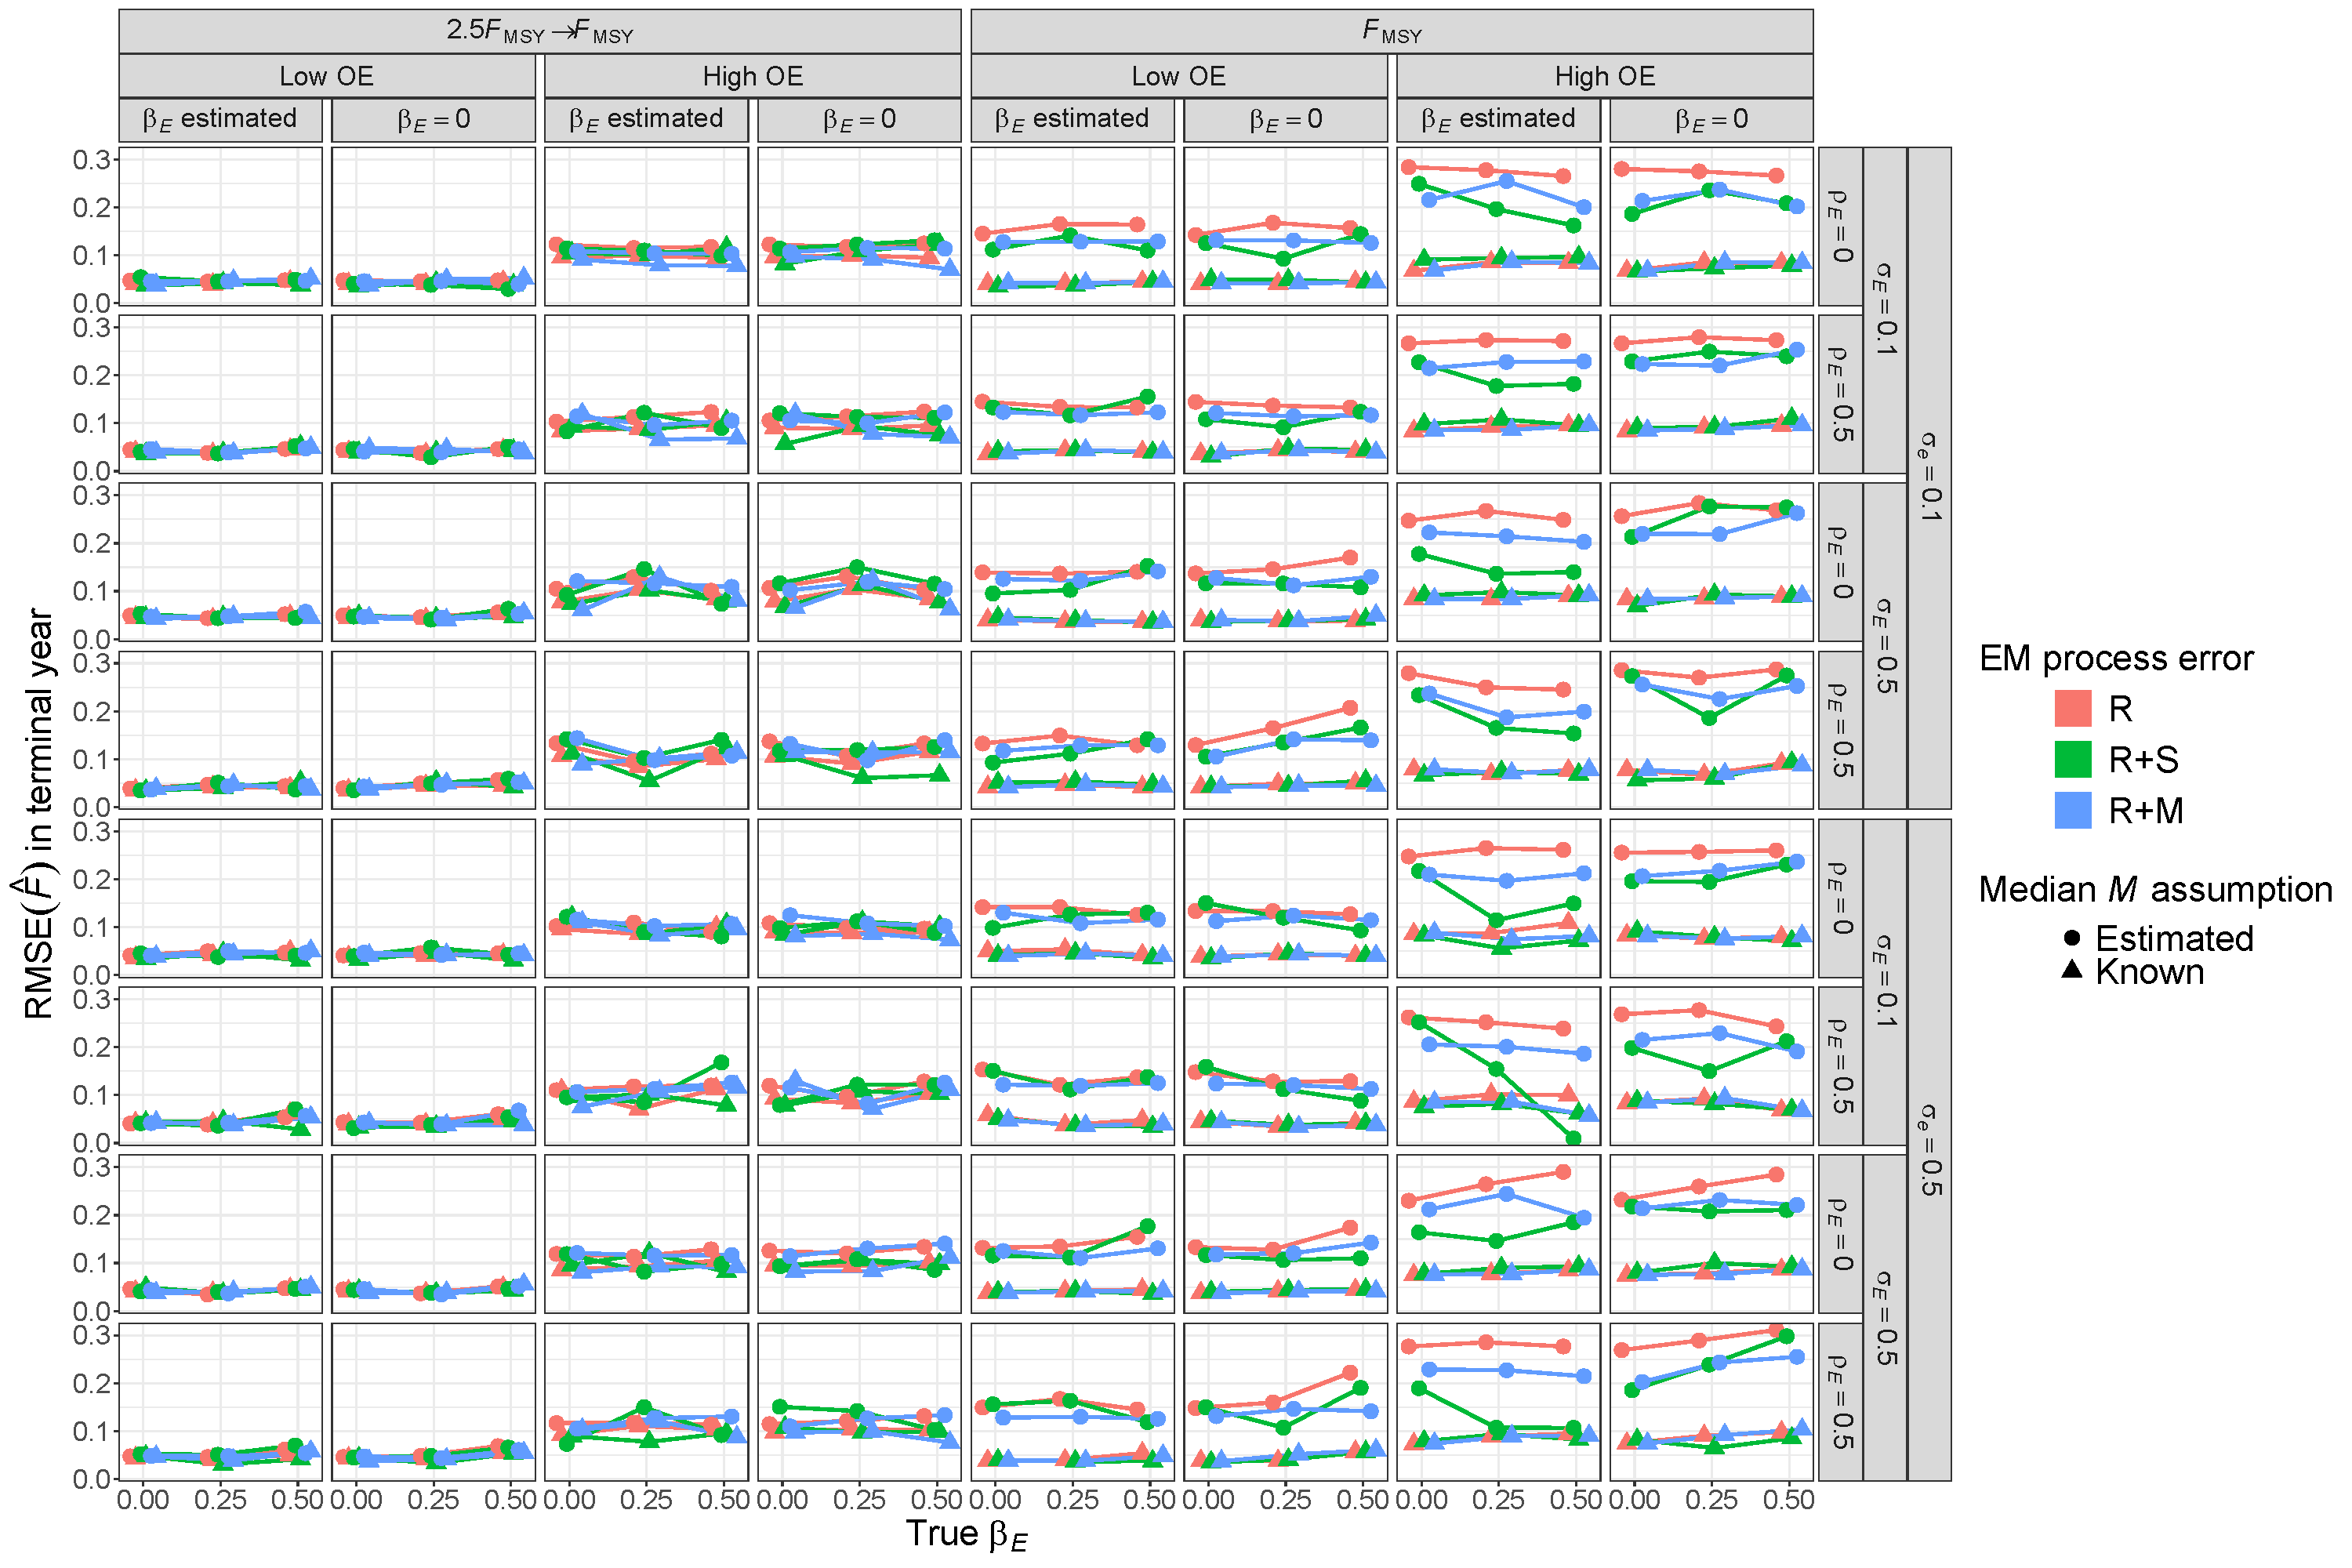
\includegraphics[height = \textheight]{terminal_year_F_rmse_Rom}
\end{center}
\caption{For R OMs, \DIFdelbeginFL \DIFdelFL{root mean square error (}\DIFdelendFL RMSE \DIFdelbeginFL \DIFdelFL{) }\DIFdelendFL of estimates of fully-selected fishing mortality ($F$)  in the terminal year for EMs with alternative process error assumptions, treatment of covariate effect ($\beta_E = 0$ or estimated), and treatment of median \DIFdelbeginFL \DIFdelFL{natural mortality }\DIFdelendFL \DIFaddbeginFL \DIFaddFL{$M$ }\DIFaddendFL parameter ($\beta_M$ estimated or known).}\label{terminal_F_rmse_Rom}
\end{figure}
\end{landscape}

\begin{landscape}
\begin{figure}
\begin{center}
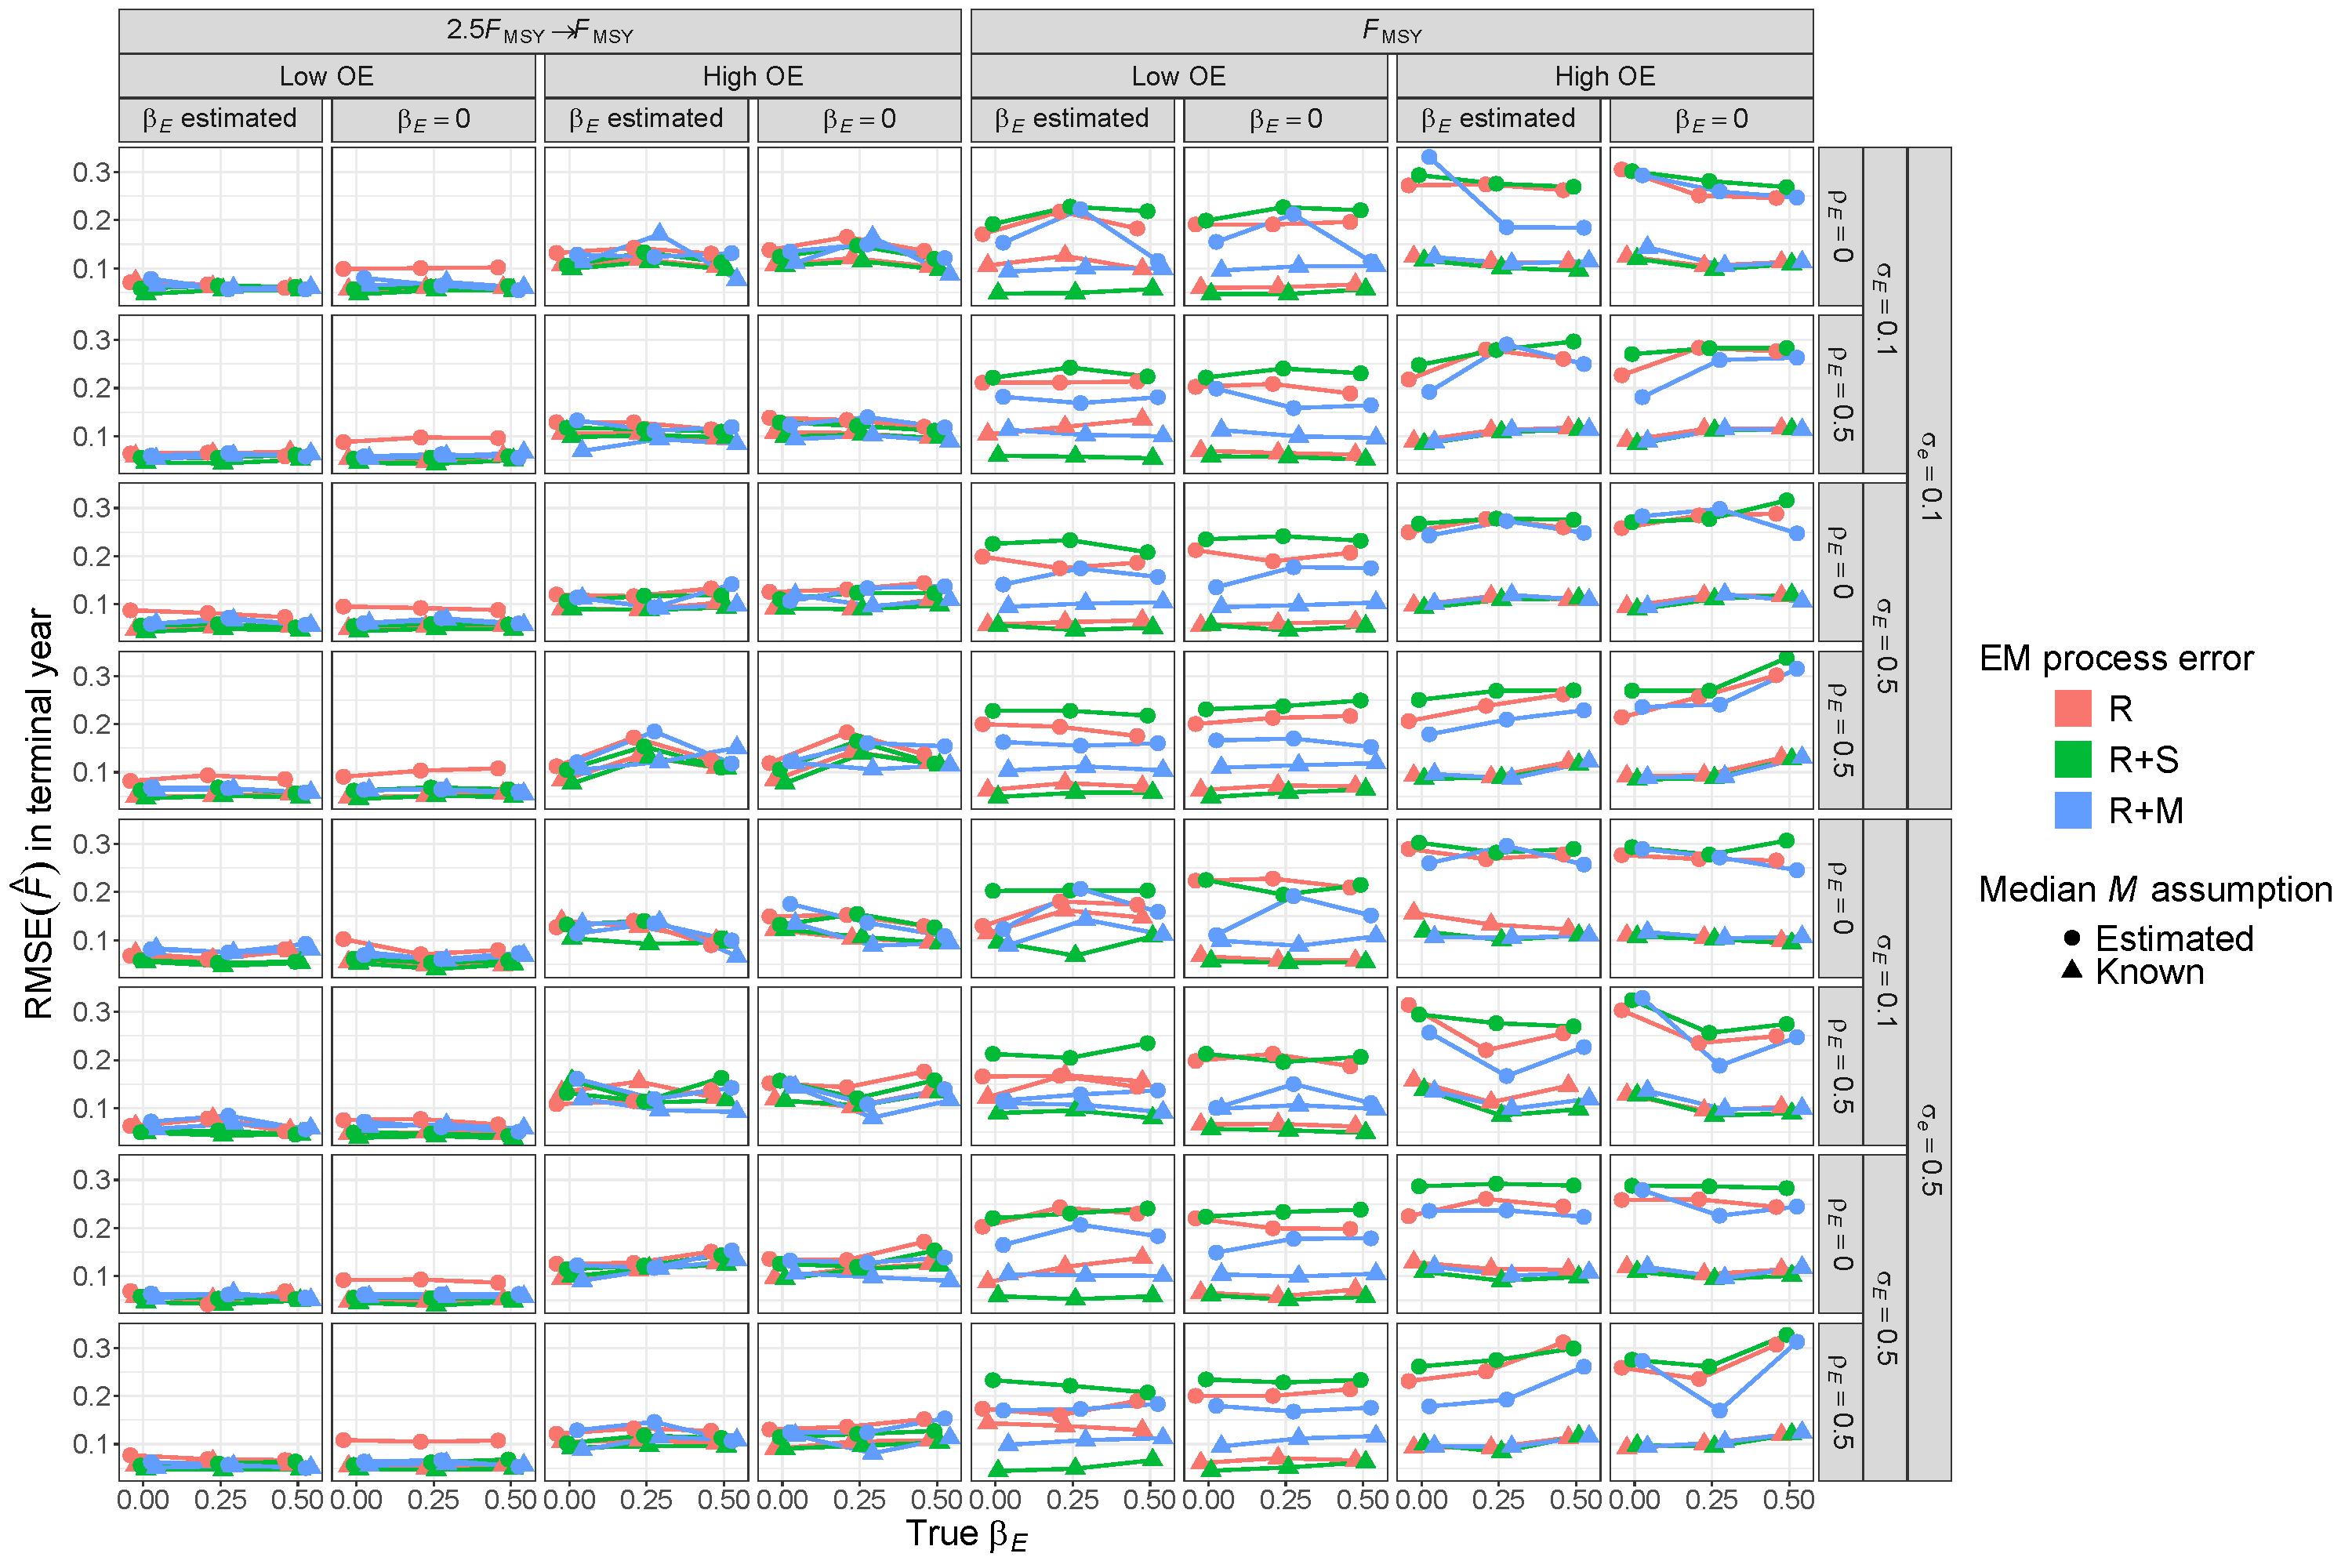
\includegraphics[height = \textheight]{terminal_year_F_rmse_RSom}
\end{center}
\caption{For R+S OMs, \DIFdelbeginFL \DIFdelFL{root mean square error (}\DIFdelendFL RMSE \DIFdelbeginFL \DIFdelFL{) }\DIFdelendFL of estimates of fully-selected fishing mortality ($F$)  in the terminal year for EMs with alternative process error assumptions, treatment of covariate effect ($\beta_E = 0$ or estimated), and treatment of median \DIFdelbeginFL \DIFdelFL{natural mortality }\DIFdelendFL \DIFaddbeginFL \DIFaddFL{$M$ }\DIFaddendFL parameter ($\beta_M$ estimated or known).}\label{terminal_F_rmse_RSom}
\end{figure}
\end{landscape}

\begin{landscape}
\begin{figure}
\begin{center}
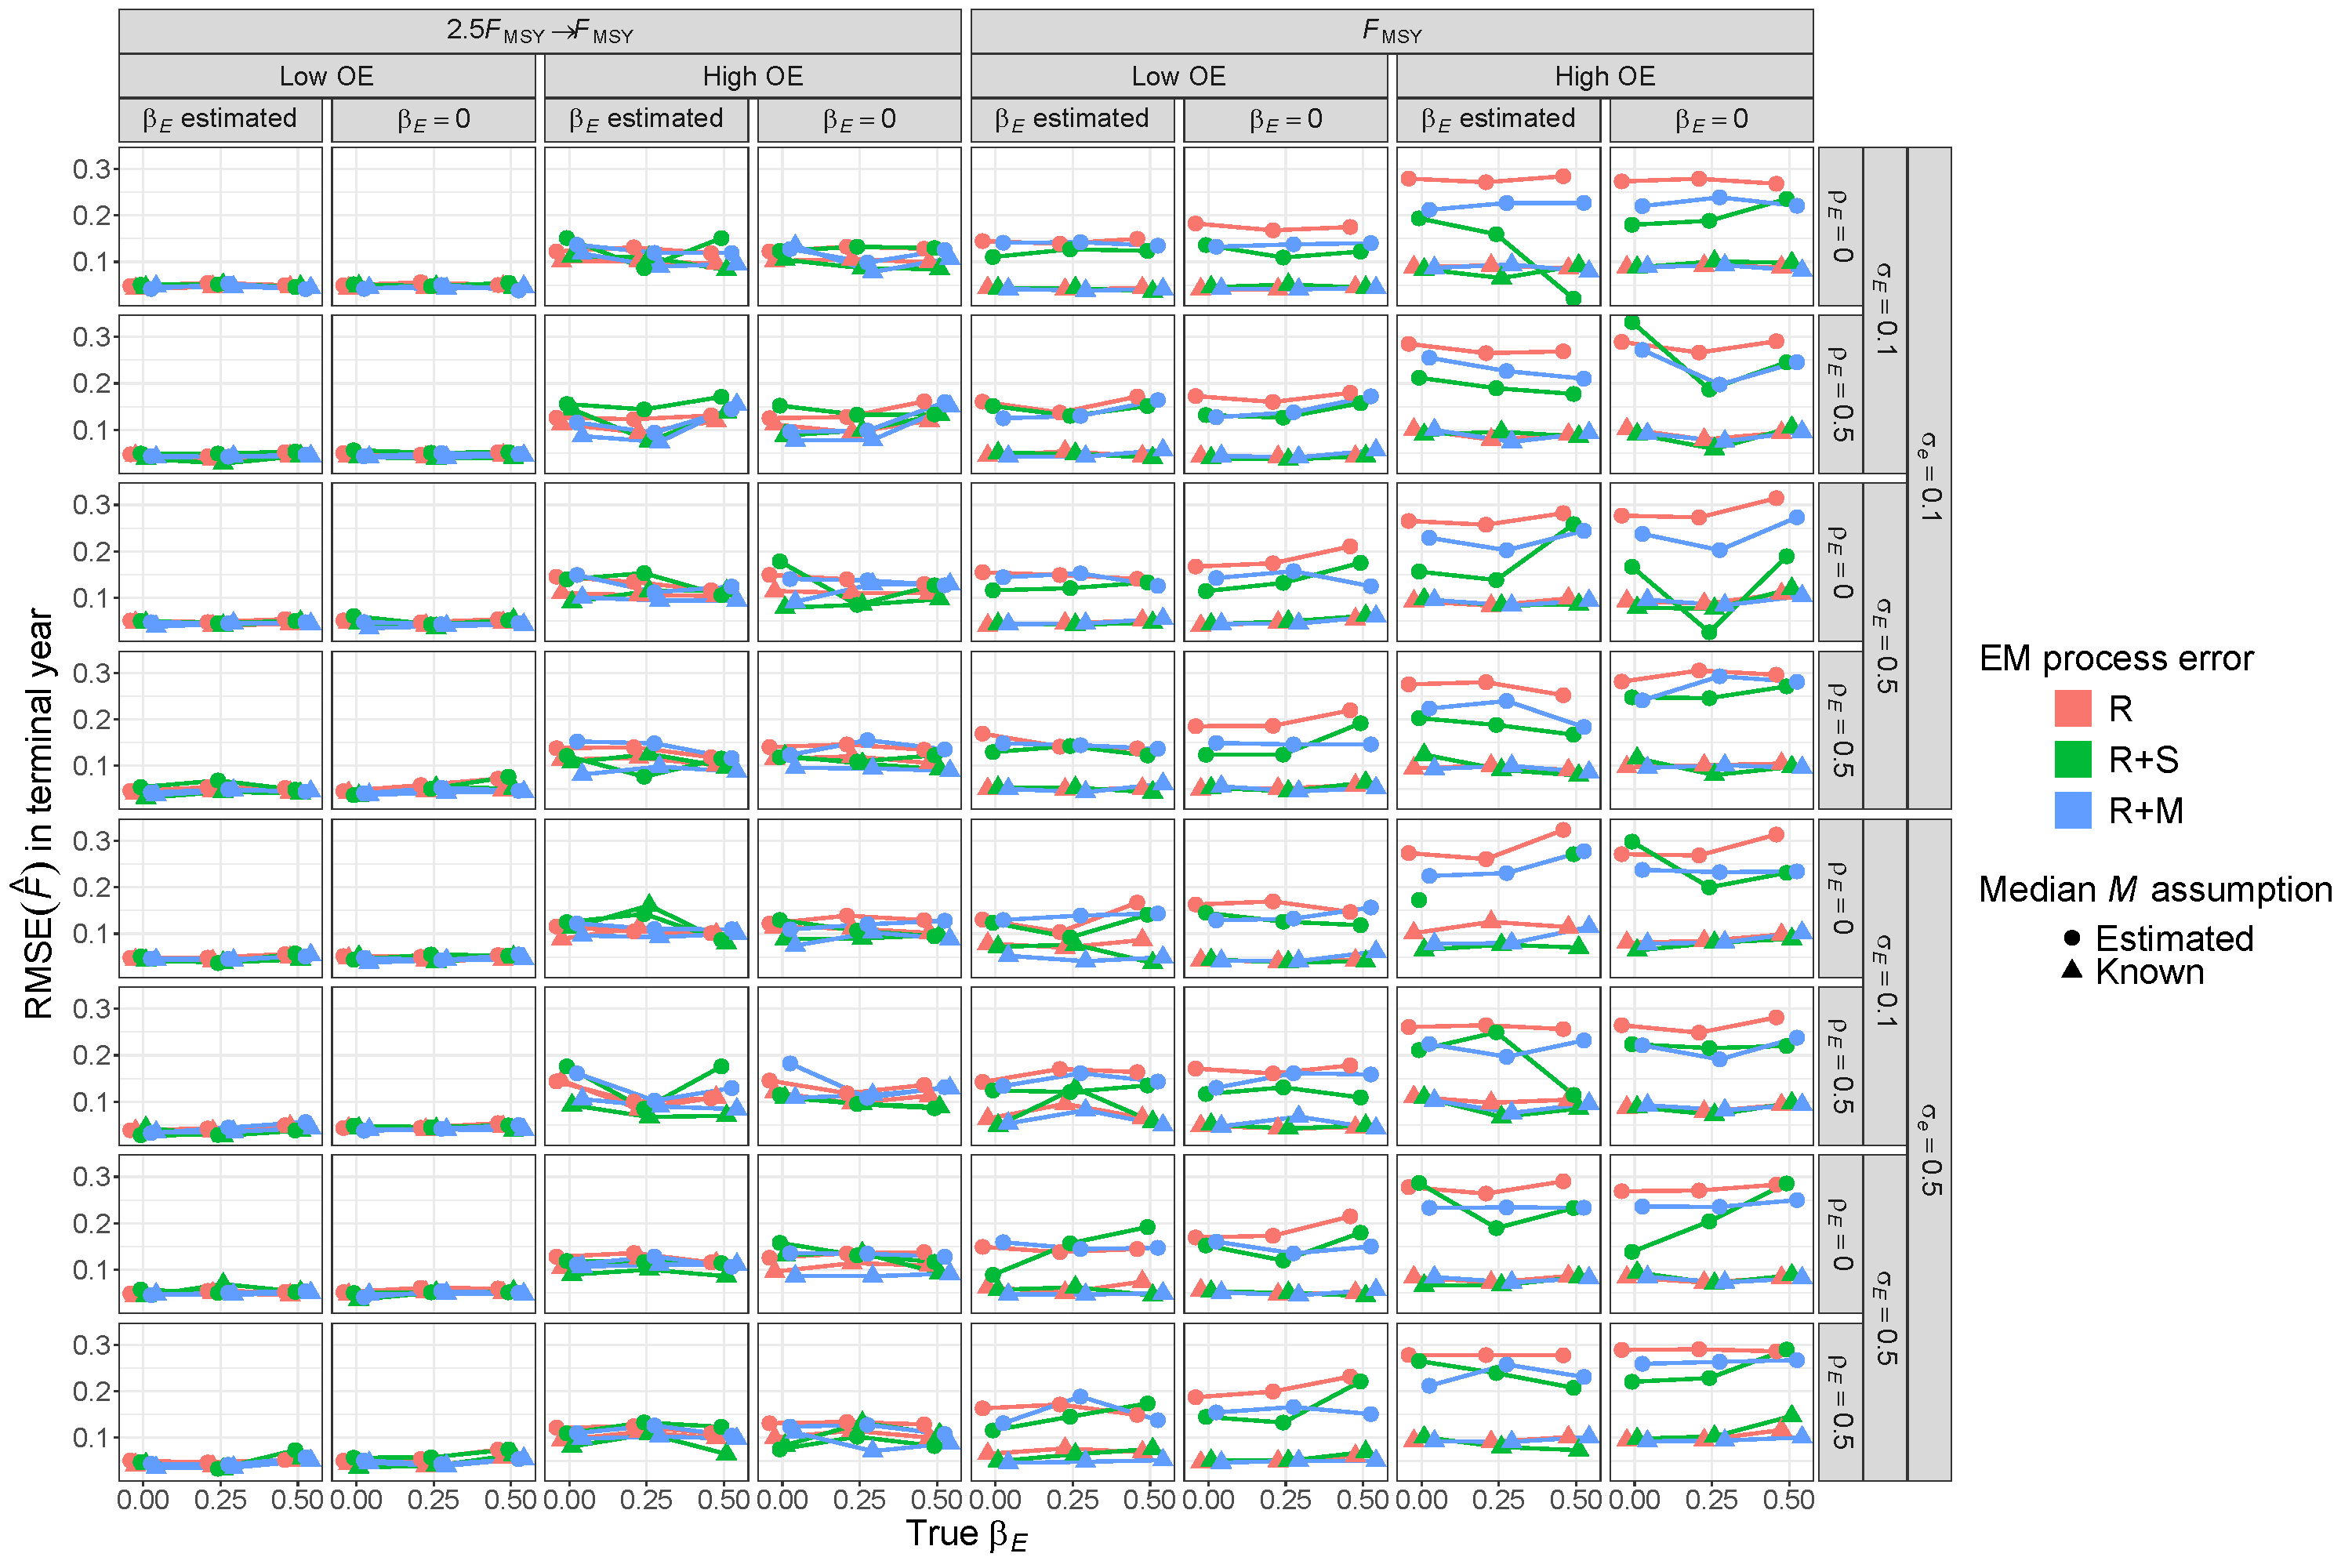
\includegraphics[height = \textheight]{terminal_year_F_rmse_RMom}
\end{center}
\caption{For R+M OMs, \DIFdelbeginFL \DIFdelFL{root mean square error (}\DIFdelendFL RMSE \DIFdelbeginFL \DIFdelFL{) }\DIFdelendFL of estimates of fully-selected fishing mortality ($F$)  in the terminal year for EMs with alternative process error assumptions, treatment of covariate effect ($\beta_E = 0$ or estimated), and treatment of median \DIFdelbeginFL \DIFdelFL{natural mortality }\DIFdelendFL \DIFaddbeginFL \DIFaddFL{$M$ }\DIFaddendFL parameter ($\beta_M$ estimated or known).}\label{terminal_F_rmse_RMom}
\end{figure}
\end{landscape}

\end{document}
